\documentclass[twocolumn
  %,draft
]{svjour3}

%\acmConference[CONF]{Conference}{2022}{USA}
%\settopmatter{printfolios=true} % print page numbers

%\usepackage[a-2b]{pdfx}
\usepackage{amsmath}
\usepackage{amsfonts}
\usepackage[utf8]{inputenc}
\usepackage{array}
\usepackage{stmaryrd}
\usepackage{tikz}
\usepackage{comment}
\usepackage{xspace}
\usepackage{listofitems}
\usepackage{graphicx}
\usepackage[final]{listings}
\usepackage{enumitem}
%\usepackage{amsthm}
\usepackage{ifthen}
\usepackage{hyperref}

% space saving tricks
\newif\ifstreamexamples
\streamexamplestrue
\newif\ifzsetexamples
\zsetexamplestrue
%\titlespacing{\paragraph}{0pt}{0pt}{1em}
%\titlespacing{\section}{0pt}{*.9}{*.9}
%\titlespacing{\subsection}{0pt}{*.9}{*.9}
\widowpenalty=0
\clubpenalty=0
%\newtheoremstyle{note} % name
%{2pt} % Space above
%{2pt} % Space below
%{}    % Body font
%{}    % Indent amount
%{\bfseries} % Theorem head font
%{:}   % Punctuation after theorem head
%{.5em}% ⟨Space after theorem head
%{}    % Theorem head spec (can be left empty, meaning ‘normal’

\numberwithin{equation}{section}

\graphicspath{ {.} }
\lstset{basicstyle=\ttfamily}
\lstset{language=Java,
  commentstyle=\color{brown},
  keywordstyle=\color{blue},
  stringstyle=\color{red},
  basicstyle=\ttfamily}

\lstdefinelanguage{ddlog}{
  language=Java, % we base it on Java, just for comments
  morekeywords={input, output, typedef, relation, typedef, bool, not,
    string, bit, extern, function, var, for, match, skip, in, integer, % not really in DDlog
    Aggregate, FlatMap},
  deletestring=[b]{'}
}
\hypersetup{
  colorlinks   = true,    % Colours links instead of ugly boxes
  urlcolor     = blue,    % Colour for external hyperlinks
  linkcolor    = blue,    % Colour of internal links
  citecolor    = red      % Colour of citations
}
\hypersetup{final}

\usetikzlibrary{shapes, arrows.meta, positioning, decorations.pathreplacing, matrix}
\tikzstyle{block}=[draw,fill=white,rectangle]
\tikzstyle{every node}=[font=\small]

%\theoremstyle{note}
%\newtheorem{theorem}{Theorem}[section]
%\newtheorem{lemma}[theorem]{Lemma}
%\newtheorem{corollary}[theorem]{Corollary}
%\newtheorem{definition}[theorem]{Definition}
%\newtheorem{proposition}[theorem]{Proposition}
%\newtheorem{example}[theorem]{Example}
\newtheorem{algorithm}[theorem]{Algorithm}
\newcommand{\dbsp}{DBSP\xspace}

%\newcommand{\anonymize}[1]{#1}
% Used when a term is first defined.  Adds the term to the index.
\newcommand{\defined}[1]{\textbf{#1}\index{}}
\newcommand{\zr}{$\Z$-set\xspace}
\newcommand{\zrs}{$\Z$-sets\xspace} % plural
\newcommand{\means}[1]{\ensuremath{\llbracket #1 \rrbracket}}
\newcommand{\code}[1]{\mbox{\texttt{#1}}}
\newcommand{\Z}{\mathbb{Z}}  % integers
\newcommand{\N}{\mathbb{N}}  % naturals
\newcommand{\B}{\mathbb{B}}  % Booleans
\newcommand{\R}{\mathbb{R}}  % reals
% stream with elements of a given type
\newcommand{\stream}[1]{\ensuremath{\mathcal{S}_{#1}}}
% finite stream with elements of a given type (zero almost everywhere)
\newcommand{\streamf}[1]{\ensuremath{\overline{\mathcal{S}_{#1}}}}
\newcommand{\zm}{\ensuremath{z^{-1}}} % stream delay operator
\ifthenelse{\equal{1}{1}}{ % allows switching to mathit/mathcal
\newcommand{\I}{\mathcal{I}}  % stream integration
\newcommand{\D}{\mathcal{D}}  % stream derivative
}{
\newcommand{\I}{\mathit{I}}  % stream integration
\newcommand{\D}{\mathit{D}}  % stream derivative
}
\newcommand{\inc}[1]{{#1}^{\Delta}}
\newcommand{\distinct}{\mathit{dist}}  % distinct operator
% set with elements of given type
\newcommand{\secref}[1]{\S\ref{#1}}  % reference to a section
\newcommand{\refsec}[1]{\secref{#1}}
\newcommand{\set}[1]{\mathit{set}_{#1}}
\newcommand{\id}{\ensuremath{\mathit{id}}} % identity function
\newcommand{\isset}{\mbox{isset}}
\newcommand{\ispositive}{\mbox{ispositive}}
\newcommand{\defn}{\stackrel{\textrm{\scriptsize def}}{=}}
\newcommand{\map}{\mbox{map}}
\newcommand{\fix}[2]{\mbox{fix}\,#1.#2}
\newcommand{\lift}[1]{{\uparrow}#1}
\newcommand{\rew}{\ensuremath{\mapsto}} % rewriting
\newcommand{\birew}{\ensuremath{\mapsfrom\!\mapsto}} % bidirectional rewriting
\newcommand{\pair}[2]{\ensuremath{\langle #1,#2 \rangle}} % pairing
\newcommand{\norm}[1]{\| #1 \|} % norm; requires math mode
%\newcommand{\zpp}[1]{\mbox{zpp}(#1)}
\newcommand{\makeset}{\ensuremath{\mbox{\texttt{UPSERT}}}}
\newcommand{\sv}[1]{ % simple stream value, supplied as a space-separated list of 5 values
\setsepchar{ }
\readlist\arg{#1}
\begin{tabular}{|c|c|c|c|c|} \hline
  % notice that this is in reverse
  \!\ensuremath{\cdots}\! &
  \!\arg[4]\! &
  \!\arg[3]\! &
  \!\arg[2]\! &
  \!\arg[1]\!
  % \arg[5] &
  \\ \hline
\end{tabular}
}

\title{\dbsp: Automatic Incremental View Maintenance for Rich Query Languages}

\author{Mihai Budiu
  \and Leonid Ryzhyk
  \and Gerd Zelwegger
  \and Ben Pfaff
  \and Lalith Suresh
  \and Abhinav Gyawali
  \and Matei Budiu
  \and Tej Chajed
  \and Frank McSherry
  \and Val Tannen}

\institute{Mihai Budiu, Leonid Ryzhyk, Gerd Zellweger, Ben Pfaff,
  Lalith Suresh, Abhinav Gyawali, Matei Budiu \at Feldera.com
  \and
  Tej Chajed \at University of Wiconsin-Madison
  \and
  Frank McSherry \at Materialize.com
  \and
  Val Tannen \at University of Pennsylvania
}

\begin{document}

\maketitle

\begin{abstract}
Incremental view maintenance (IVM) has long been a central problem in
database theory and practice.  Many solutions have been proposed for
restricted classes of database languages (such as the relational
algebra or Datalog), restricted classes of queries, and restricted
classes of database changes.  In this paper we give a general,
heuristic-free solution to this problem in 4 steps: (1) we describe a
simple but expressive language called \dbsp for describing
computations over data streams; (2) we give a new mathematical
definition of IVM using \dbsp; (3) we give a general algorithm for
converting any \dbsp program into an incremental program; this
algorithm reduces the problem of incrementalizing a complex query to
the problem of incrementalizing the primitive operations that compose
the query.  Finally, (4) we show that practical database query
languages, such as SQL and Datalog, can be directly implemented on top
of \dbsp, using primitives that have efficient incremental
implementations.  As a consequence, we obtain a general recipe for
efficient IVM for essentially arbitrary queries written in all these
languages.

\end{abstract}

\section{Introduction}\label{sec:introduction}

Incremental view maintenance (IVM) is an important and well-studied
problem in databases~\cite{gupta-idb95}.  The IVM problem can be
stated as follows: we are given a large database $DB$ (say 1 billion
records) and a view $V$, described by a query $Q$.  The goal of IVM is
to keep the contents of $V$ up-to-date in response to changes of the
database.

As a concrete example, consider the following view definition
statement in SQL:

\texttt{CREATE VIEW V AS SELECT * FROM T WHERE Age >= 10}.

In this example the query $Q$ defining the view $V$ is
\\ \texttt{SELECT * FROM T WHERE Age >= 10}.  The view \code{V} always
contains all the rows of table \code{T} whose value for the column
\code{Age} is greater or equal to 10.

In general a query is a function applied to the database state: $V =
Q(DB)$.  A naive solution is to re-execute query $Q$ every time the
database changes (or every time someone wants to inspect the view's
content).  In the following diagram we illustrate the naive solution.
Time is the horizontal axis; the horizontal arrows labeled with
$\Delta$ depict changes to the database, which we assume are much
smaller than the database itself (e.g., a change could touch perhaps
100 records).  The ``up'' arrows show the re-evaluation of $Q$ for
each database snapshot.

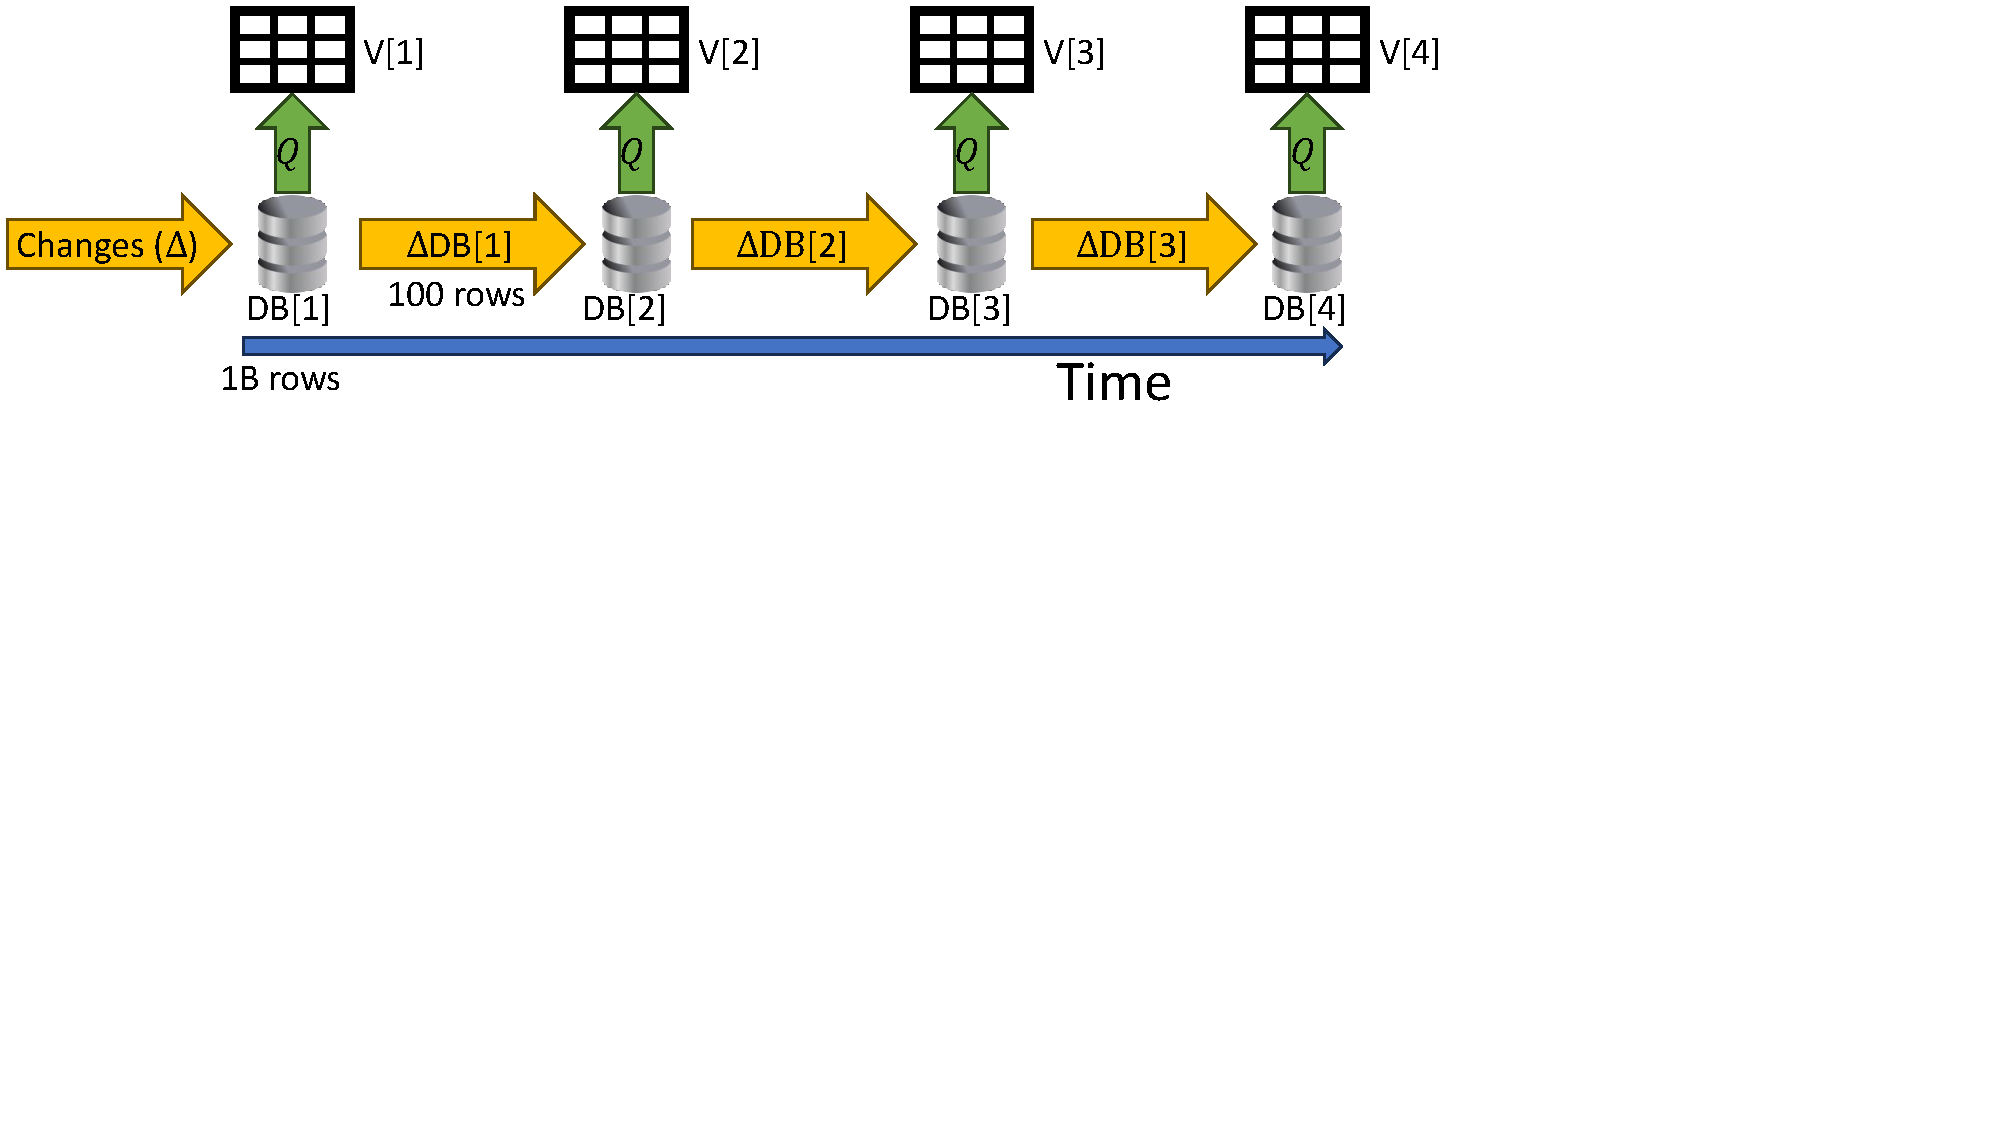
\includegraphics[trim={0 3.8in 4in 0},clip,scale=.3]{view.pdf}

The naive solution is expensive.  After the first version of the view
has been constructed, the ideal algorithm computes only \emph{changes}
to the view $\Delta V$ by performing work proportional to $O(|\Delta
DB|)$.  Ideally, we want to construct a new query $\inc{Q}$ with the
property that $\Delta V = \inc{Q}(\Delta DB)$, i.e., $\inc{Q}$ can
compute the change of the view from the change of the database:

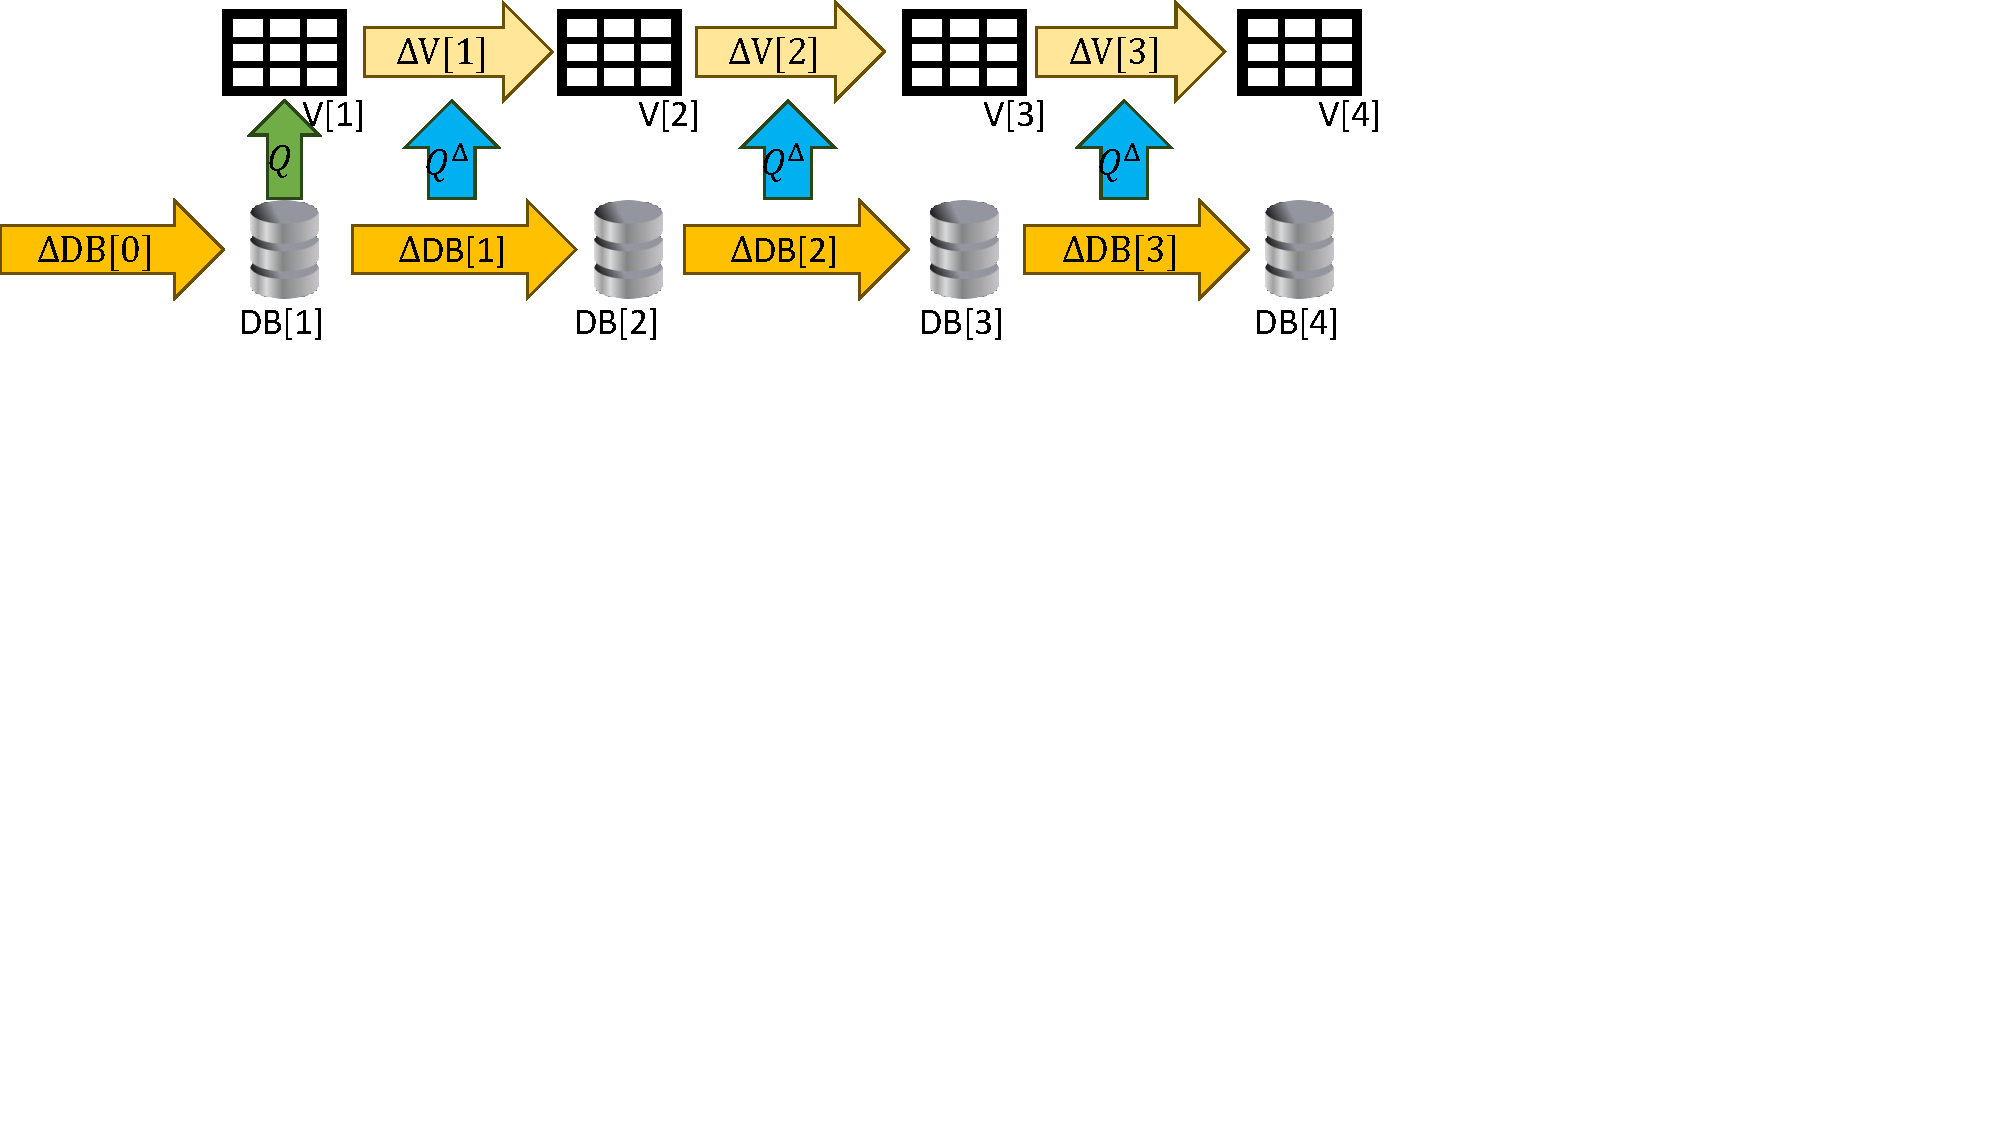
\includegraphics[trim={0 4in 4in 0},clip,scale=.3]{incview.pdf}

We call $\inc{Q}$ the \emph{incremental} version of $Q$.  This paper
provides a new perspective on this problem by proposing a new
definition of IVM based on a streaming model of computation.  Our
model is inspired by Digital Signal Processing
DSP~\cite{rabiner-book75}, applied to databases, hence the name \dbsp.

In general it is not possible to compute $\Delta V$ only as a function
of $\Delta DB$, so $\inc{Q}$ also needs to look at $DB$.  For
essentially all practical queries $Q$ we give an algorithm to
construct a corresponding query $\inc{Q}(DB, \Delta DB)$, which
computes $\Delta V$, and which is faster than $Q$ by a factor of \\
$O(|DB| / |\Delta DB|)$.

Instead of treating the database as a monolithic changing object, we
treat it as a \emph{sequence} or \emph{stream} of database snapshots.
Similarly, the view snapshots form a stream.  \dbsp is a simple
programming language for computing on streams; the inputs and outputs
of \dbsp programs are streams of arbitrary values.

%Whereas previous IVM solutions are based on defining a notion of a
%(partial) derivative of $Q$ with respect to its inputs, our definition
%only requires computing \emph{derivatives of streams} as functions of
%time.  Derivatives of streams are always well-defined if the data
%computed on has a notion of difference that satisfies some simple
%mathematical properties --- specifically, that it forms a commutative
%group.  (Fortunately, relational databases can be modeled in such a
%way~\cite{green-pods07, koch-pods10}.)

The \dbsp language has only 4 operators.  However, it can express a
rich set of computations on streams, including repeated computations
(similar to the repeated queries $Q$ above), recursive computations
that compute fixed points (as done by Datalog programs), streaming
computations, and incremental computations (which we define shortly).
The full paper~\cite{budiu-vldb23} gives a precise mathematical
description of \dbsp, this presentation is simplified to convey the
main intuitions behind the design.  We omit the related work section
from this presentation.

The central result of this paper is algorithm~\ref{algorithm-inc}
which, given a \dbsp program that computes on a stream of values,
mechanically transforms it into an incremental \dbsp program that
computes on a stream of changes.

\dbsp is not tied to databases in any way; it is in fact a
Turing-complete language that can be used for many other purposes.
But it works particularly well in the area of databases, for two
reasons:

\begin{itemize}
  \item \dbsp operates on values that must have nice mathematical
    properties (it requires the values in a stream to belong to a
    commutative group).  Databases can be modeled as values from a
    commutative group.
  \item \dbsp reduces the problem of incrementalizing a complex
    program to the problem of incrementalizing each primitive
    operation that appears in the program.  For the domain of
    databases there are known efficient incremental implementations
    for all primitive operations.
\end{itemize}

%\dbsp has several attractive properties:
%
%\begin{enumerate}
%\item it is \textbf{simple}.  \dbsp has only 4 operators, and it is
%  built entirely on elementary concepts such as functions and
%  algebraic groups.
%\item it is \textbf{expressive}.  It can be used to define precisely
%  multiple concepts: traditional queries, streaming computations, and
%  incremental computations.
%\item mathematically \textbf{precise}.  All the results in this paper
%  have been formalized and checked using the Lean proof
%  assistant~\cite{moura-cade15}.
%\item it is \textbf{modular}, in the following two ways:
%(a) the incremental version of a complex query can be reduced
%recursively to incrementalizing its component subqueries.
%This gives a simple, syntactic,
%heuristic-free algorithm (Algorithm~\ref{algorithm-inc})
%that converts an arbitrary \dbsp query plan to its incremental form.
%(b) Extending \dbsp to support new primitive operators is easy,
%and they immediately benefit from the rest of the theory of
%incrementalization.
%An important consequence of modularity is that the theory
%can be efficiently implemented, as we
%briefly discuss in \refsec{sec:implementation}.
%\end{enumerate}

\subsection{Databases as streams}

The core concept of \dbsp is the \emph{stream}, which is used to model
changes of an object over time.  $\stream{A}$ is the type of
(infinite) streams with values of type $A$. If $s \in \stream{A}$ is a
stream, then $s[t]$ is the $t$-th element of $s$, also referred to as
the \emph{value of the stream at time $t$}.  A streaming operator is a
function that consumes one or more streams and produces another
stream.  We show streaming computations with diagrams, also called
``circuits'', where boxes are computations and streams are arrows with
double heads.  The following diagram shows a stream operator $T$
consuming two input streams $s_0$ and $s_1$ and producing one output
stream $s$:

\begin{center}
\begin{tikzpicture}[auto,>=latex,minimum width=.5cm]
  \node[] (input0) {$s_0$};
  \node[below of=input0,node distance=.3cm] (dummy) {};
  \node[below of=dummy,node distance=.3cm] (input1) {$s_1$};
  \node[block, right of=dummy] (T) {$T$};
  \node[right of=T] (output) {$s$};
  \draw[->>] (input0) -- (T);
  \draw[->>] (input1) -- (T);
  \draw[->>] (T) -- (output);
\end{tikzpicture}
\end{center}

All our stream computations are ``causal'': the output at time $t$ is
produced immediately after the inputs at time $t$ have been received.

We generally think of streams as sequences of ``small'' values, such
as insertions or deletions in a database.  However, we also treat the
whole database as a \emph{stream of database snapshots}.  We model a
database as a stream $DB$.  Time is not wall-clock time, but counts
the transactions applied to the database.  Since transactions are
linearizable, they have a total order.  $DB[t]$ is the snapshot of the
database contents after $t$ transactions have been applied.

Database transactions also form a stream $\Delta DB$, this time a
stream of \emph{changes}, or \emph{deltas} that are applied to the
database.  The values of this stream are defined by $(\Delta DB)[t] =
DB[t] - DB[t-1]$, where ``$-$'' stands for the difference between two
databases, a notion that we will soon make more precise.  The $\Delta
DB$ stream can be produced from the $DB$ stream by the \emph{stream
differentiation} operator $\D$; this operator produces as its output
the stream of changes from its input stream; we have thus $\D(DB) =
\Delta DB$.

Conversely, the database snapshot at time $t$ is the cumulative result
of applying all transactions up to $t$: $DB[t] = \Delta DB[0] + \Delta
DB[1] + \ldots + \Delta DB[t]$.  The stream operator $\I$ is defined
to produce an output by adding up all previous inputs.  We call this
operator \emph{stream integration}, the inverse of differentiation.
The following diagram shows the relationship between the streams
$\Delta DB$ and $DB$:
\begin{center}
\begin{tikzpicture}[auto,>=latex,minimum width=.5cm, node distance=1.2cm]
  \node[] (input) {$\Delta DB$};
  \node[block, right of=input] (I) {$\I$};
  \node[right of=I] (output) {$DB$};
  \node[block, right of=output] (D) {$\D$};
  \node[right of=D] (end) {$\Delta DB$};
  \draw[->>] (input) -- (I);
  \draw[->>] (I) -- (output);
  \draw[->>] (output) -- (D);
  \draw[->>] (D) -- (end);
\end{tikzpicture}
\end{center}

Suppose we are given a query $Q$ defining a view $V$.  What is a view
in our streaming model?  It is also a stream!  For each snapshot of
the database stream we have a snapshot of the view: $V[t] = Q(DB[t])$.
In general, given an arbitrary function $f: A \to B$, we define a
streaming ``version'' of $f$, denoted by $\lift{f}$ (read as ``$f$
lifted''), which applies $f$ to every element of the input stream
independently.  We can thus write $V = (\lift{Q})(DB)$.

Armed with these basic definitions, we can precisely define IVM.  What
does it mean to maintain a view incrementally?  A maintenance
algorithm needs to compute the \emph{changes} to the view given the
changes to the database. Given a query $Q$, a key contribution of this
paper is the definition of its \emph{incremental version} $\inc{Q}$,
using stream integration and differentiation, depicted graphically as:

\begin{center}
\begin{tikzpicture}[auto,>=latex,minimum width=.5cm]
  \node[] (input) {$\Delta DB$};
  \node[block, right of=input] (I) {$\I$};
  \node[block, right of=I, node distance=1.3cm] (Q) {$\lift{Q}$};
  \node[block, right of=Q, node distance=1.3cm] (D) {$\D$};
  \node[right of=D] (output) {$\Delta V$};
  \draw[->>] (input) -- (I);
  \draw[->>] (I) -- node (db) {$DB$} (Q);
  \draw[->>] (Q) -- node (B) {$V$} (D);
  \draw[->>] (D) -- (output);
  \draw[decorate, decoration = {brace, raise=13pt}] (input) -- (output)
  node[pos=.5, above=13pt]{$\inc{Q}$};
\end{tikzpicture}
\end{center}

The incremental version of a query $Q$ is a stateful \emph{streaming
operator} $\inc{Q}$ which computes directly on changes and produces
changes.  The incremental version of a query is thus always
well-defined.  The above definition also gives us one way to compute a
query incrementally, but applying it naively produces an inefficient
execution plan, since it will reconstruct the database at each step.
It is in fact as bad as the naive solution.  In
\refsec{sec:incremental} we show how we can optimize the
implementation of $\inc{Q}$. The key property is that the incremental
composition of two queries $Q_1$ and $Q_2$ is the composition of their
incremental versions: $\inc{(Q_1 \circ Q_2)} = \inc{Q_1} \circ
\inc{Q_2}$.

Armed with this general theory of incremental computation, in
\secref{sec:relational} we show how to model relational queries in
\dbsp.  This immediately gives us a general algorithm to compute the
incremental version of any relational query.  These results were
previously known, but they are cleanly modeled by \dbsp.
\secref{sec:recursion} shows how programs containing recursion can be
implemented and incrementalized in \dbsp.  For example, given an
implementation of transitive closure in the natural recursive way, our
algorithm produces a program that efficiently maintains the transitive
closure of a graph as the graph is changed by adding and deleting
nodes and edges.

\subsection{Contributions}

This work makes the following contributions:
\begin{enumerate}
  \item \dbsp, a \textbf{simple} but \textbf{expressive} language for streaming
  computation. \dbsp gives an elegant formal foundation unifying the manipulation of
  streaming and incremental computations.
  \item An algorithm for incrementalizing any streaming computation expressed in
  \dbsp.
  \item An illustration of how \dbsp can model various classes of
    practical queries, such as relational algebra, nested relations,
    aggregations, and Datalog.
  \item The first general and machine-checked theory of IVM.  All the
    theoretical results in this paper have been checked using the Lean
    proof assistant~\cite{dbsp-theory}.
  \item Practical open-source implementations of this theory as a
    runtime and a SQL compiler.
\end{enumerate}


\section{Stream computations}\label{sec:streams}

The core notion of our theory of IVM is the \textbf{stream}.  In this
section we introduce streams as infinite sequences of values, and
define computations on streams.

\subsection{Streams and stream operators}\label{sec:notation}

$\N$ is the set of natural numbers (from 0), $\B$ is the set of
Booleans, $\Z$ is the set of integers, and $\R$ is the set of real
numbers.

\begin{definition}[stream]
Given a set $A$, a \defined{stream} \emph{of values from $A$}, or an
\emph{$A$-stream}, is a function $\N \rightarrow A$.  We denote by
$\stream{A} \defn \{ s \,|\, s : \N \to A \}$ the set of all
$A$-streams.
\end{definition}

When $s\in\stream{A}$ and $t\in\N$ we
write $s[t]$ for the $t$-th element of the stream $s$.

\begin{definition}[stream operator]
A \defined{stream operator} is a function
$T:\stream{A_0}\times\cdots\times\stream{A_{n-1}}\to\stream{B}$.
\end{definition}

\begin{definition}(lifting)
Given a (scalar) function $f: A \to B$,
we define a stream operator $\lift{f} :\stream{A} \to \stream{B}$
by \emph{lifting} the function $f$ pointwise in time: $(\lift{f})(s) \defn f \circ s$.
Equivalently, $((\lift{f})(s))[t] \defn f(s[t])$.
This extends to functions of multiple arguments.
\end{definition}

\ifstreamexamples
For example, $(\lift{(\lambda x.(2x))})(id) = \sv{0 2 4 6 8}$.
\fi

\begin{proposition}[distributivity]\label{prop:distributivity}
Lifting distributes over function composition:
$\lift{(f \circ g)} = (\lift{f}) \circ (\lift{g})$.
\end{proposition}
\begin{comment}
\begin{proof}
This is easily proved by using associativity of function composition:
$\forall s~.~(\lift{(f \circ g)})(s) = (f \circ g) \circ s =
f \circ (g \circ s) = f \circ (\lift{g})(s) = (\lift{f})((\lift{g})(s)) =
(\lift{f} \circ \lift{g})(s).$
\end{proof}
\end{comment}

We say that two \dbsp programs are \defined{equivalent} if they compute the same
input-output function on streams.
We use the symbol $\cong$ to indicate that two circuits are
equivalent.  For example, Proposition~\ref{prop:distributivity}
states the following circuit equivalence:

\noindent
\begin{tabular}{m{3.5cm}m{.3cm}m{3.5cm}}
\begin{tikzpicture}[auto,>=latex]
  \node[] (input) {$s$};
  \node[block, right of=input] (g) {$\lift{g}$};
  \node[block, right of=g] (f) {$\lift{f}$};
  \node[right of=f] (output) {$o$};
  \draw[->>] (input) -- (g);
  \draw[->>] (g) -- (f);
  \draw[->>] (f) -- (output);
\end{tikzpicture}
&
$\cong$
&
\begin{tikzpicture}[auto,>=latex]
    \node[] (input) {$s$};
    \node[block, right of=input, node distance=1.5cm] (fg) {$\lift{(f \circ g)}$};
    \node[right of=fg, node distance=1.5cm] (output) {$o$};
    \draw[->>] (input) -- (fg);
    \draw[->>] (fg) -- (output);
\end{tikzpicture}
\end{tabular}

\subsection{Streams over abelian groups}\label{sec:abelian}

For the rest of the technical development we require the set of values
$A$ of a stream $\stream{A}$ to form a commutative group $(A, +, 0_A,
-)$.  The \emph{plus} defines what it means to add new data, while the
\emph{minus} allows us to compute differences (deltas).  We show later
that this restriction is not a problem for using \dbsp with relational
data.

\subsubsection{Delays and time-invariance}\label{sec:delay}

\begin{definition}[Delay]
The \defined{delay operator}\footnote{The name $\zm$ comes from the
DSP literature, and is related to the
z-transform~\cite{rabiner-book75}.}  $\zm$ produces an output stream
by delaying its input by one step: $\zm_A: \stream{A} \to \stream{A}$:
%\begin{tabular}{m{5cm}m{3cm}}
$$
\zm_A(s)[t] \defn   \begin{cases}
0_A      & \text{when}~t=0 \\
s[t - 1] & \text{when}~t\geq1
\end{cases}
$$
%&
%\begin{tikzpicture}[auto,node distance=1cm,>=latex]
%    \node[] (input) {$s$};
%    \node[block, right of=input] (z) {$\zm$};
%    \node[right of=z] (output) {$o$};
%    \draw[->] (input) -- (z);
%    \draw[->] (z) -- (output);
%\end{tikzpicture}
%\end{tabular}
\end{definition}

We often omit the type parameter $A$, and write just $\zm$.
\ifstreamexamples
For example, $\zm(\id) = \sv{0 0 1 2 3}$.
\fi

\begin{definition}[Time invariance]
A stream operator $S: \stream{A} \to \stream{B}$ is \defined{time-invariant} (TI) if
$S(\zm_A(s)) = \zm_B(S(s))$ for all $s \in \stream{A}$; in other words, if
the following two circuits are equivalent:

\begin{tabular}{m{3cm}m{.5cm}m{3cm}}
\begin{tikzpicture}[auto,>=latex]
  \node[] (input) {$s$};
  \node[block, right of=input] (S) {$S$};
  \node[block, right of=S] (z) {$\zm$};
  \node[right of=z] (output) {$o$};
  \draw[->>] (input) -- (S);
  \draw[->>] (S) -- (z);
  \draw[->>] (z) -- (output);
\end{tikzpicture}
&
$\cong$
&
\begin{tikzpicture}[auto,>=latex]
  \node[] (input) {$s$};
  \node[block, right of=input] (z) {$\zm$};
  \node[block, right of=z] (S) {$S$};
  \node[right of=S] (output) {$o$};
  \draw[->>] (input) -- (z);
  \draw[->>] (z) -- (S);
  \draw[->>] (S) -- (output);
\end{tikzpicture}
\end{tabular}
\end{definition}

The output of a TI operator only depends on its input, but never on
the ``logical clock'' value.  For example the operator $S(s)[t] = s[t]
+ t$ is \emph{not} TI.  The composition of TI operators of any number
of inputs is TI. The delay operator $\zm$ is TI.  \dbsp only uses TI
operators.

%\begin{definition}
%We say that a function between groups $f: A \to B$ has the \emph{zero-preservation
%property} if $f(0_A) = 0_B$.  We write $\zpp{f}$.
%\end{definition}
%
%A lifted operator $\lift{f}$ is TI iff $\zpp{f}$.

\subsubsection{Causal and strict operators}\label{sec:causal}

The definitions in this section are used to argue that some circuits
with cycles are well-defined.

\begin{definition}[Causality]
A stream operator \\ $S:\stream{A}\to\stream{B}$
is \defined{causal} when $\forall s,s'\in\stream{A}$,
and $\forall t \in \N$ we have:
$
(\forall i \leq t~.~s[i]=s'[i]) \Rightarrow S(s)[t]=S(s')[t].
$
\end{definition}

\noindent
In other words, the output value at time $t$ can only depend on input
values from times $t' \leq t$ (they cannot ``look'' into the future).
Operators produced by lifting are causal, and $\zm$ is causal.  The
composition of causal operators is causal.  \dbsp only uses causal
operators.

\begin{definition}[Strictness]
A stream operator \\ $F:\stream{A}\to\stream{B}$
is \defined{strict}
if  $\forall s,s'\in\stream{A}, \forall t \in \N$ we have:
$(\forall i<t~.~s[i]=s'[i]) \Rightarrow F(s)[t]=F(s')[t].$
\end{definition}

In other words, the $t$-th output of $F(s)$ can depend only on
``past'' values of the input $s$, between $0$ and $t-1$.  In
particular, $F(s)[0] = 0_B$ is the same for all $s \in \stream{A}$.
Strict operators are causal, but in addition, the current output can
only depend on previous inputs.  Lifted operators in general are
\emph{not} strict.  $\zm$ is strict.  Strict operators can compute
their $k$-th output before having received their corresponding input.

\begin{proposition}
\label{prop-unique-fix}
For a strict $F: \stream{A} \to \stream{A}$ the equation ~$\alpha=F(\alpha)$~ has a unique
solution $\alpha \in \stream{A}$, denoted by $\fix{\alpha}{F(\alpha)}$.
\end{proposition}

Thus every strict operator from a set to itself has a unique fixed
point.  The simple proof relies on strong induction, showing that the
solution $\alpha[t]$ depends only on the values of $\alpha$ prior to
$t$.

Consider a circuit with a strict ``feedback'' edge $F$:
\begin{center}
\begin{tikzpicture}[>=latex]
    \node[] (input) {$s$};
    \node[block, right of=input] (f) {$T$};
    \node[right of=f, node distance=1.2cm] (output) {$\alpha$};
    \node[block, below of=f, node distance=.6cm] (z) {$F$};
    \draw[->>] (input) -- (f);
    \draw[->>] (f) -- node (mid) {} (output);
    \draw[->>] (mid.center) |-  (z);
    \draw[->>] (z.west) -- ++(-.4,0) |- ([yshift=1mm]f.south west);
\end{tikzpicture}
\end{center}

This circuit is a well-defined function on streams, because the $F$
operator can produce an output before having received the
corresponding input, enabling $T$ to compute the first output
immediately.

%\begin{lemma}
%\label{lemma-causal-strict}
%If $F: \stream{B} \to \stream{B}$ is strict and $T: \stream{A} \times \stream{B} \to \stream{B}$ is causal, then for fixed $s$ the operator
%$\lambda\alpha.T(s,F(\alpha)): \stream{A} \to \stream{B}$ is strict.
%\end{lemma}

\begin{lemma}\label{feedback-semantics}
\label{cor-loop}
If $F: \stream{B} \to \stream{B}$ is strict and $T: \stream{A} \times \stream{B} \to \stream{B}$ is causal,
the operator $Q(s)=\fix{\alpha}{T(s,F(\alpha))}$ is well-defined and causal.
If, moreover, $F$ and $T$ are TI then so is $Q$.
\end{lemma}

Most \dbsp computations are built using just lifted functions and
delays.  We add two more operators in \secref{sec:nested} to support
recursive functions.

\subsection{Integration and differentiation}\label{sec:abelianstreams}

Remember that we require the elements of a stream to come from an abelian group $A$.
Streams themselves form an abelian group:

\begin{proposition}
The structure $(\stream{A},+,0,-)$, obtained by lifting the $+$ and unary $-$ operations of $A$,
is an abelian group.  0 is the stream with all values $0_A$.
\end{proposition}

\noindent
To simplify the notation, we write $a + b$ for streams $a, b$ instead
of $a (\lift{+}) b$; we also write $-a$ instead of $(\lift{-})a$.
Stream addition and negation are causal, TI operators.

\begin{definition}
Given abelian groups $A$ and $B$ we call a stream operator
$S: \stream{A} \rightarrow \stream{B}$ \defined{linear} if it is a group homomorphism, that is,
$S(a+b)=S(a)+S(b)$ (and therefore $S(0)=0$ and $S(-a)=-S(a)$).
\end{definition}

We write LTI for ``linear and TI''.  Given a linear function $f: A \to
B$, the stream operator $\lift{f}$ is LTI.  $\zm$ is also LTI.

\begin{definition}(bilinear)
A function of two arguments $f: A \times B \to C$ where $A, B, C$ are
groups, is \emph{bilinear} if it is linear separately in each argument
(i.e., it distributes over addition): $\forall a, b, c, d~.~f(a+b, c)
= f(a, c) + f(b, c)$, and $f(a, c+d) = f(a, c) + f(c, d).$
\end{definition}

This definition extends to stream operators.
The lifting of a bilinear function $f$ is
a bilinear stream operator $\lift{f}$.  An example
is lifted multiplication:
$f: \stream{\N} \times \stream{\N} \to \stream{\N}, f(a, b)[t] = a[t]\cdot b[t]$.

%The composition of (bi)linear operators with linear operators
%is (bi)linear (since homomorphisms compose).

\begin{definition}[Differentiation]
The \defined{differentiation operator} $\D_{\stream{A}} : \stream{A}
\to \stream{A}$ is: $\D(s) \defn s - \zm(s)$.
\begin{center}
\begin{tikzpicture}[auto,>=latex,node distance=1cm]
    \node[] (input) {$s$};
    \node[block, shape=circle, right of=input, inner sep=0pt,node distance=2cm] (plus) {$+$};
    \node[right of=plus] (output) {$\D(s)$};
    \draw[->>] (input) -- node (i) {} (plus);
    \node[block, below of=i, node distance=.8cm] (z) {$\zm$};
    \node[block, shape=circle, right of=z, inner sep=0pt] (minus) {$-$};
    \draw[->>] (plus) -- (output);
    \draw[->>] (i) -- (z);
    \draw[->>] (z) -- (minus);
    \draw[->>] (minus) -- (plus);
\end{tikzpicture}
\end{center}
\end{definition}
We generally omit the type, and write just $\D$.
The value of $\D(s)[t] = s[t] - s[t-1]$ if $t > 0$.
If $s$ is a stream, then $\D(s)$ is the \emph{stream of changes} of $s$.

As an example:
{
\noindent \small
\begin{align*}
  &\D(\sv{0 1 2 1 0}) &= \\
  &\sv{0 1 2 1 0} - \zm(\sv{0 1 2 1 0}) &=\\
  &\sv{0 1 2 1 0} - \sv{0 0 1 2 1} &=\\
%  &\sv{0-0 1-0 2-1 1-2 0-1} =\\
  &\sv{0 1 1 -1 -1}
\end{align*}
}

\begin{proposition}
\label{prop-diff-properties}
$\D$ is causal and LTI.
\end{proposition}

The ``feedback loop'' built from linear operator and a delay is
linear:

\begin{proposition}
\label{prop-rec-linear}
Let $S$ be a unary, causal, LTI operator. The
operator $Q(s)=\fix{\alpha}{S(s+\zm(\alpha))}$ is well-defined and LTI:

\begin{center}
\begin{tikzpicture}[>=latex]
    \node[] (input) {$s$};
    \node[block, shape=circle, right of=input, inner sep=0pt, node distance=.8cm] (plus) {$+$};
    \node[block, right of=plus, node distance=.8cm] (Q) {$S$};
    \node[right of=Q, node distance=1.4cm] (output) {$\alpha$};
    \node[block, below of=Q, node distance=.6cm] (z) {$\zm$};
    \draw[->>] (input) -- (plus);
    \draw[->>] (plus) -- (Q);
    \draw[->>] (Q) -- node (mid) {} (output);
    \draw[->>] (mid.center) |-  (z);
    \draw[->>] (z) -| (plus);
\end{tikzpicture}
\end{center}
\end{proposition}

The integration operator ``reconstitutes'' a stream from its changes:

\begin{definition}[Integration]
The \defined{integration operator} $\I_{\stream{A}} : \stream{A} \to
\stream{A}$ is $\I(s) \defn \lambda s . \fix{\alpha}{(s +
  \zm(\alpha))}$:
\begin{center}
\begin{tikzpicture}[auto,>=latex, node distance=1.1cm]
    \node[] (input) {s};
    \node[block, shape=circle, right of=input, inner sep=0pt] (plus) {$+$};
    \node[right of=plus, node distance=1.9cm] (output) {$\I(s) = o$};
    \node[block, below of=plus, node distance=.8cm] (z) {$z^{-1}$};
    \draw[->>] (input) -- (plus);
    \draw[->>] (plus) -- node (o) {} (output);
    \draw[->>] (o) |- (z);
    \draw[->>] (z) -- (plus);
\end{tikzpicture}
\end{center}
\end{definition}

\noindent
We also omit the type, and write just $\I$.  This is the circuit from
Proposition~\ref{prop-rec-linear} using the identity for $S$.

\begin{proposition}
$\I(s)$ is the discrete (indefinite) integral applied to the stream $s$:
$\I(s)[t] = \sum_{i \leq t} s[i]$.
\end{proposition}
\begin{proof}
Using the notation $o = \I(s)$ to make formulas more readable, we can
see the contents of stream $o$ is produced step by step.  Here are the
first three steps:
\begin{align*}
  o[0] &= s[0] + (\zm(o))[0] = s[0] + 0 = s[0] \\
  o[1] &= s[1] + (\zm(o))[1] = s[1] + o[0] = s[1] + s[0] \\
  o[2] &= s[2] + (\zm(o))[2] = s[2] + o[1] = s[2] + (s[1] + s[0])
\end{align*}
\end{proof}

\begin{proposition}
\label{prop-integ-properties}
$\I$ is causal and LTI.
\end{proposition}

\begin{theorem}[Inversion]
\label{inverses}
$\I$ and $\D$ are inverses of each other: $\forall s~.~\I(\D(s)) =
\D(\I(s)) = s$.
\end{theorem}

\noindent
\begin{tabular}{m{2.5cm}m{.2cm}m{.8cm}m{.2cm}m{2.5cm}}
\begin{tikzpicture}[auto,>=latex, node distance=.85cm]
    \node[] (input) {$s$};
    \node[block, right of=input] (I) {$\I$};
    \node[block, right of=I] (D) {$\D$};
    \node[right of=D] (output) {$o$};
    \draw[->>] (input) -- (I);
    \draw[->>] (I) -- (D);
    \draw[->>] (D) -- (output);
\end{tikzpicture}
     & $\cong$ &
\begin{tikzpicture}[auto,>=latex, node distance=.85cm]
    \node[] (input) {$s$};
    \node[right of=input] (output) {$o$};
    \draw[->>] (input) -- (output);
\end{tikzpicture}
     & $\cong$ &
\begin{tikzpicture}[auto,>=latex, node distance=.85cm]
    \node[] (input) {$s$};
    \node[block, right of=input] (D) {$\D$};
    \node[block, right of=D] (I) {$\I$};
    \node[right of=I] (output) {$o$};
    \draw[->>] (input) -- (D);
    \draw[->>] (D) -- (I);
    \draw[->>] (I) -- (output);
\end{tikzpicture}
\end{tabular}

\section{Incremental view maintenance}\label{sec:incremental}

Here we define IVM and analyze its properties.

\begin{definition}
Given a unary stream operator $Q: \stream{A} \to \stream{B}$ we define the
\defined{incremental version} of $Q$ as:
\begin{equation}\label{def:inc}
\inc{Q} \defn \D \circ Q \circ \I.
\end{equation}
$\inc{Q}$ has the same ``type'' as $Q$: $\inc{Q}: \stream{A} \to \stream{B}$.
For an operator with multiple inputs we define
the incremental version by applying $\I$ to each input independently:
e.g., if $T: \stream{A} \times \stream{B} \rightarrow \stream{C}$ then
$\inc{T}(a, b) \defn \D (T(\I(a), \I(b)))$.
\end{definition}

%The following diagram illustrates the intuition behind this
%definition:
\begin{center}
\begin{tikzpicture}[auto,>=latex]
    \node[] (input) {$\Delta s$};
    \node[block, right of=input] (I) {$\I$};
    \node[block, right of=I] (Q) {$Q$};
    \node[block, right of=Q] (D) {$\D$};
    \node[right of=D] (output) {$\Delta o$};
    \draw[->>] (input) -- (I);
    \draw[->>] (I) -- node (s) {$s$} (Q);
    \draw[->>] (Q) -- node (o) {$o$} (D);
    \draw[->>] (D) -- (output);
    \draw[decorate, decoration = {brace, raise=10pt}] (input) -- (output)
    node[pos=.5, above=13pt]{$\inc{Q}$};
\end{tikzpicture}
\end{center}
If $Q(s) = o$ is a streaming operator, then $\inc{Q}$ operates on
streams of changes: $\inc{Q}(\Delta s) = \Delta o$.

Notice that our definition of incremental computation is meaningful only for \emph{streaming}
computations; this is in contrast to classic definitions, e.g.~\cite{gupta-idb95} which
consider only one change.  Generalizing the definition to operate on streams gives us
additional power, especially when operating with recursive queries.

The following is one of our central results:

\begin{proposition}(Properties of the incremental version):
\label{prop-inc-properties}
\begin{description}[nosep, leftmargin=\parindent]
\item[inversion:] $Q\mapsto\inc{Q}$ is bijective; its inverse is $Q\mapsto \I\circ Q\circ\D$.
\item[invariance:] $\inc{+} = +, \inc{(\zm)} = \zm, \inc{-} = -, \inc{\I}=\I, \inc{\D}=\D$
\item[push/pull:] \label{prop-part-commutation}
    $Q \circ \I = \I \circ \inc{Q}$; $\D\circ Q = \inc{Q}\circ\D$
\item[chain:] $\inc{(Q_1\circ Q_2)} = \inc{Q_1}\circ\inc{Q_2}$
\item[add:] $\inc{(Q_1 + Q_2)} = \inc{Q_1} + \inc{Q_2}$
\item[cycle:] $\inc{(\lambda s. \fix{\alpha}{T(s,\zm(\alpha)}))} = \lambda s. \fix{\alpha}{\inc{T}(s,\zm(\alpha)})$
\end{description}
\end{proposition}

Here is the proof of the \defined{chain rule}, which states that
$\inc{(Q_1 \circ Q_2)} = \inc{Q_1} \circ \inc{Q_2}$.

\begin{tabular}{cr}
\begin{tikzpicture}[auto,>=latex]
  \node[] (input) {$\Delta i$};
  \node[block, right of=input] (I) {$\I$};
  \node[block, right of=I] (Q1) {$Q_1$};
  \node[block, right of=Q1] (Q2) {$Q_2$};
  \node[block, right of=Q2] (D) {$\D$};
  \node[right of=D] (output)  {$\Delta o$};
  \draw[->>] (input) -- (I);
  \draw[->>] (I) -- (Q1);
  \draw[->>] (Q1) -- (Q2);
  \draw[->>] (Q2) -- (D);
  \draw[->>] (D) -- (output);
\end{tikzpicture} &
$\cong$ \\
\begin{tikzpicture}[>=latex, node distance=.9cm]
  \node[] (input) {$\Delta i$};
  \node[block, right of=input] (I1) {$\I$};
  \node[block, right of=I1] (Q1) {$Q_1$};
  \node[block, right of=Q1] (D1) {$\D$};
  \node[block, right of=D1] (I2) {$\I$};
  \node[block, right of=I2] (Q2) {$Q_2$};
  \node[block, right of=Q2] (D2) {$\D$};
  \node[right of=D2] (output)  {$\Delta o$};
  \draw[->>] (input) -- (I1);
  \draw[->>] (I1) -- (Q1);
  \draw[->>] (Q1) -- (D1);
  \draw[->>] (D1) -- (I2);
  \draw[->>] (I2) -- (Q2);
  \draw[->>] (Q2) -- (D2);
  \draw[->>] (D2) -- (output);
\end{tikzpicture} &
$\cong$ \\
\begin{tikzpicture}[>=latex, node distance=1.2cm]
  \node[] (input) {$\Delta i$};
  \node[block, right of=input] (Q1) {$\inc{Q_1}$};
  \node[block, right of=Q1] (Q2) {$\inc{Q_2}$};
  \node[right of=Q2] (output)  {$\Delta o$};
  \draw[->>] (input) -- (Q1);
  \draw[->>] (Q1) -- (Q2);
  \draw[->>] (Q2) -- (output);
\end{tikzpicture}
\end{tabular}

\noindent In other words, \textbf{to incrementalize a composite query you can incrementalize
each sub-query independently}.  This gives us a simple, syntax-directed, deterministic recipe
for computing the incremental version of an arbitrarily complex query.

The \defined{cycle rule} states that the following circuits are equivalent:

\noindent
\begin{tabular}{m{4.4cm}m{.2cm}m{3cm}}
\begin{tikzpicture}[>=latex]
    \node[] (input) {$\Delta s$};
    \node[block, right of=input] (I) {$\I$};
    \node[block, right of=I] (f) {$T$};
    \node[block, right of=f, node distance=1.4cm] (D) {$\D$};
    \node[right of=D] (output) {$\Delta o$};
    \node[block, below of=f, node distance=.6cm] (z) {$\zm$};
    \draw[->>] (input) -- (I);
    \draw[->>] (I) -- (f);
    \draw[->>] (f) -- node (mid) {} (D);
    \draw[->>] (mid.center) |-  (z);
    \draw[->>] (z.west) -- ++(-.3,0) |- ([yshift=1mm]f.south west);
    \draw[->>] (D) -- (output);
\end{tikzpicture} & $\cong$ &
\begin{tikzpicture}[>=latex]
    \node[] (input) {$\Delta s$};
    \node[block, right of=input] (f) {$\inc{T}$};
    \node[right of=f, node distance=1.3cm] (output) {$\Delta o$};
    \node[block, below of=f, node distance=.6cm] (z) {$\zm$};
    \draw[->>] (input) -- (f);
    \draw[->>] (f) -- node (mid) {} (output);
    \draw[->>] (mid.center) |-  (z);
    \draw[->>] (z.west) -- ++(-.3,0) |- ([yshift=1mm]f.south west);
\end{tikzpicture}
\end{tabular}

In other words, the incremental version of a feedback loop around a
query is just the feedback loop with the incremental query for its
body.  This result will be used to implement recursive queries
in~\refsec{sec:recursion}.

To execute incremental queries efficiently, we want to compute directly
on streams of changes, without integrating them. The invariance property above shows
that stream operators $+$, $-$, and $\zm$ are identical to their incremental versions.
The following theorems extend this to linear and bi-linear operators:

\begin{theorem}[Linear]\label{linear}
If $Q$ is LTI, we have $\inc{Q}=Q$.
\end{theorem}

\begin{theorem}[Bilinear]\label{bilinear}
Using the infix notation: if $\times$ is bilinear TI, we have:
\begin{eqnarray*}
\inc{(\Delta a \times \Delta b)} = \\
(\Delta a \times \Delta b ~+~ \zm(\I(\Delta a)) \times
\Delta b ~+~ \Delta a \times \zm(\I(\Delta b)) = \\
\Delta a \times \Delta b + \zm(a) \times \Delta b + \Delta a \times \zm(b)
\end{eqnarray*}
In pictures: \\
\noindent
\begin{tabular}{m{3.3cm}m{0cm}m{4cm}}
\begin{tikzpicture}[auto,>=latex]
    \node[] (a) {$\Delta a$};
    \node[block, right of=a] (ai) {$\I$};
    \node[below of=a, node distance=.8cm] (midway) {};
    \node[below of=midway, node distance=.8cm] (b) {$\Delta b$};
    \node[block, right of=b] (bi) {$\I$};
    \node[block, right of=midway, node distance=1cm] (q) {$\times$};
    \node[block, right of=q] (D) {$\D$};
    \node[right of=D] (output) {$\Delta o$};
    \draw[->>] (a) -- (ai);
    \draw[->>] (b) -- (bi);
    \draw[->>] (ai) -- (q);
    \draw[->>] (bi) -- (q);
    \draw[->>] (q) -- (D);
    \draw[->>] (D) -- (output);
\end{tikzpicture} &
$\cong$ &
\begin{tikzpicture}[auto,>=latex]
  \node[] (input1) {$\Delta a$};
  \node[below of=input1, node distance=1.6cm] (input2) {$\Delta b$};
  \node[block, right of=input1, node distance=1cm] (I1) {$\I$};
  \node[block, below of=I1,node distance=.8cm] (ab) {$\times$};
  \node[block, right of=input2, node distance=1cm] (I2) {$\I$};
  \draw[->>] (input1) -- (I1);
  \draw[->>] (input2) -- (I2);
  \draw[->>] (input1) |- ([yshift=-1mm]ab.north west);
  \draw[->>] (input2) |- ([yshift=1mm]ab.south west);
  \node[block, right of=I1] (ZI1) {$\zm$};
  \node[block, right of=I2] (ZI2) {$\zm$};
  \draw[->>] (I1) -- (ZI1);
  \draw[->>] (I2) -- (ZI2);
  \node[block, right of=ZI1] (DI1) {$\times$};
  \node[block, right of=ZI2] (DI2) {$\times$};
  \draw[->>] (ZI1) -- (DI1);
  \draw[->>] (ZI2) -- (DI2);
  \node[block, circle, right of=ab, inner sep=0cm, node distance=2cm] (sum) {$+$};
  \draw[->>] (ab) -- (sum);
  \draw[->>] (DI1) -- (sum);
  \draw[->>] (DI2) -- (sum);
  \node[right of=sum, node distance=.8cm] (output) {$\Delta o$};
  \draw[->>] (sum) -- (output);
  \draw[->>] (input1) -- (DI2);
  \draw[->>] (input2) -- (DI1);
\end{tikzpicture}
%&
%$\cong$ &
%\begin{tikzpicture}[auto,>=latex,node distance=.7cm]
%  \node[] (input1) {$a$};
%  \node[below of=input1, node distance=1cm] (input2) {$b$};
%  \node[block, right of=input1, node distance=.5cm] (I1) {$\I$};
%  \node[block, right of=input2, node distance=.5cm] (I2) {$\I$};
%  \draw[->>] (input1) -- (I1);
%  \draw[->>] (input2) -- (I2);
%  \node[block, right of=I2] (ZI2) {$\zm$};
%  \draw[->>] (I2) -- (ZI2);
%  \node[block, right of=I1] (DI1) {$\times$};
%  \node[block, right of=ZI2] (DI2) {$\times$};
%  \draw[->>] (I1) -- (DI1);
%  \draw[->>] (ZI2) -- (DI2);
%  \node[block, circle, above of=DI2, inner sep=0cm, node distance=.5cm] (sum) {$+$};
%  \draw[->>] (DI1) -- (sum);
%  \draw[->>] (DI2) -- (sum);
%  \node[right of=sum, node distance=.5cm] (output) {$o$};
%  \draw[->>] (sum) -- (output);
%  \draw[->>] (input1) -- (DI2);
%  \draw[->>] (input2) -- (DI1);
%\end{tikzpicture}
\end{tabular}
\end{theorem}

This equation is the well-known formula for join delta
queries~\cite{koch-pods10} in terms of streaming computations.


\section{IVM for the Relational Algebra}\label{sec:relational}

In this section we apply the results on incremental computation to
relational databases.  As explained in the introduction, our goal is
to efficiently compute the incremental version of any relational query
$Q$.

However, we face a technical problem: we said that streams require
their values to belong to a commutative group, and relational
databases in general are \emph{not} commutative groups, since they
operate on sets.  Fortunately, there is a well-known tool in the
database literature which converts set operations into group
operations by using \zrs (also called z-relations~\cite{green-tcs11})
to represent sets.

\subsection{\zrs}

\zrs generalize database tables: think of a \zr as a table where each
row has an associated integer weight, possibly negative.  This weight
indicates \emph{how many times} the row belongs to the table.

%Given a set $A$, we define \defined{\zrs} over $A$ as functions with
%\emph{finite support} from $A$ to $\Z$.  These are functions $f: A
%\rightarrow \Z$ where $f(x) \not= 0$ for at most a finite number of
%values $x \in A$.  We also write $\Z[A]$ for the type of \zrs with
%elements from $A$.  Values in $\Z[A]$ can be thought of as key-value
%maps with keys in $A$ and values in $\Z$, justifying the array
%indexing notation.  If $m \in \Z[A]$ we write $m[a]$ instead of
%$m(a)$, again using an indexing notation.
%
%A particular \zr $m \in \Z[A]$ can be denoted by enumerating its
%elements that have non-zero weights and their corresponding weights:
%$m = \{ x_1 \mapsto w_1, \dots, x_n \mapsto w_n \}$.
%We call $w_i \in \Z$ the \defined{weight}
%of $x_i \in A$.  Weights can be negative.
%We write that $x \in m$ iff $m[x] \not= 0$.
%We also write $w \cdot x$ for $\{ x \mapsto w \}$.

%\ifzsetexamples
%Consider a concrete \zr $R \in \Z[\texttt{string}]$,
%defined by $R = \{ \texttt{joe} \mapsto 1, \texttt{anne} \mapsto -1 \}$.
%$R$ has two elements in its domain,
%\texttt{joe} with weight 1 (so $R[\texttt{joe}] = 1$),
%and \texttt{anne} with weight $-1$.
%We say \texttt{joe} $\in R$ and \texttt{anne} $\in R$.
%\fi

The following table shows an example \zr with three rows.  The first
row has value \texttt{joe} and weight 1.  If a weight is 0 we do not
show the corresponding row.

\begin{center}
\begin{tabular}{|c|c|}\hline
  Row & Weight \\ \hline
  joe & 1 \\
  mary & 2 \\
  anne & -1 \\ \hline
\end{tabular}
\end{center}

%Since $\Z$ is an abelian ring, $\Z[A]$ is also an abelian ring (and thus a group).  This group
%$(\Z[A], +_{\Z[A]}, 0_{\Z[A]}, -_{\Z{A}})$ has addition and subtraction defined pointwise:
%$(f +_{\Z[A]} g)(x) = f(x) + g(x) . \forall x \in A.$
%The $0$ element of $\Z[A]$ is the function $0_{\Z[A]}$ defined by $0_{\Z[A]}(x) = 0 .
%\forall x \in A$.  For example, $R + R =  \{ \texttt{joe} \mapsto 2, \texttt{anne} \mapsto -2 \}$.
%Since \zrs form a group, all results from \secref{sec:streams} apply to streams over \zrs.

\zrs are more general than sets and multisets: A set can be
represented as a \zr by associating a weight of 1 with each row.
Multisets (also called ``bags'' in the database literature) are \zrs
where all weights are positive.  Crucially, \zrs can also represent
arbitrary \emph{changes} to sets and bags.  Negative weights in a
change represent rows that are being \emph{removed}.

We can define three operations on \zr of a given type (i.e., where
the values have a given type): (1) zero (with all weights 0) (2)
negation: just negate all weights; (3) plus: add up the weights of the
rows that have the same value.  Using these operations \zrs behave
like a commutative group.

%\begin{definition}
%We say that a \zr represents a \defined{set} if the weight of every
%element is one.  We define a function to check this property
%$\isset : \Z[A] \rightarrow \B$\index{isset}
%given by:
%$$\isset(m) \defn \left\{
%\begin{array}{ll}
%  \mbox{true} & \mbox{ if } m[x] = 1, \forall x \in m \\
%  \mbox{false} & \mbox{ otherwise}
%\end{array}
%\right.
%$$
%\end{definition}

%\ifzsetexamples
%For our example $\isset(R) = \mbox{false}$, since $R[\texttt{anne}] = -1$.
%\fi

%\begin{definition}
%We say that a \zr is \defined{positive} (or a \defined{bag}) if the weight of every element is
%positive.  We define a function to check this property
%$\ispositive : \Z[A] \rightarrow \B$\index{ispositive}.
%given by
%$$\ispositive(m) \defn \left\{
%\begin{array}{ll}
%  \mbox{true} & \mbox{ if } m[x] \geq 0, \forall x \in A \\
%  \mbox{false} & \mbox{ otherwise}
%\end{array}
%\right.$$
%\end{definition}
%We have $\forall m \in \Z[A] . \isset(m) \Rightarrow \ispositive(m)$.
%\ifzsetexamples
%$\ispositive(R) = \mbox{false}$, since $R[\texttt{anne}] = -1$.
%\fi
%
%We write $m \geq 0$ when $m$ is positive.  For positive $m, n \in
%\Z[A]$ we write $m \geq n$ for iff $m - n \geq 0$.  $\geq$ is a
%partial order.
%
%We call a function $f : \Z[A] \rightarrow \Z[B]$ \defined{positive} if it maps
%positive values to positive values:
%$\forall x \in \Z[A], x \geq 0_{\Z[A]} \Rightarrow f(x) \geq 0_{\Z[B]}$.
%We use the same notation for functions: $\ispositive(f)$.

%\begin{definition}[distinct]
%The function $\distinct: \Z[A] \rightarrow \Z[A]$\index{distinct}
%``converts'' a \zr into a set:
%$$\distinct(m)[x] \defn \left\{
%\begin{array}{ll}
%  1 & \mbox{ if } m[x] > 0 \\
%  0 & \mbox{ otherwise}
%\end{array}
%\right.
%$$
%%\end{definition}

We define a handy function on \zrs called $\distinct$ (this function
is called $\epsilon$ in~\cite{griffin-sigmod95}, but we use this name
because it is strongly related to the SQL \texttt{DISTINCT} operator).
This function, applied to a \zr, gives us another \zr where all
rows with negative weights are removed, and all positive weights
are changed to 1.  For example, the $\distinct$ of the above \zr is:

\begin{center}
\begin{tabular}{|c|c|}\hline
  Row & Weight \\ \hline
  joe & 1 \\
  mary & 1 \\ \hline
\end{tabular}
\end{center}

Notice that $\distinct$ ``removes'' duplicates from multisets, and it also eliminates
rows with negative weights.
%\ifzsetexamples
%$\distinct(R) = \{ \texttt{joe} \mapsto 1 \}$.
%\fi
This definition of $\distinct$ has been carefully
chosen to enable us to implement the database computations
in terms of computations on \zrs.
%Circuits derived from relational queries only compute on positive \zrs.

%\begin{definition}(mononotonicity)
%A stream $s \in \stream{\Z[A]}$ is \defined{positive} if every value of the stream is positive:
%$s[t] \geq 0 . \forall t \in \N$.
%A stream $s \in \stream{\Z[A]}$ is \defined{monotone} if $s[t] \geq s[t-1], \forall t \in \N$.
%\end{definition}
%
%If $s \in \stream{\Z[A]}$ is positive, then $\I(s)$ is monotone.
%If $s \in \stream{\Z[A]}$ is monotone, $\D(s)$ is positive.
%
%\paragraph{Functions as circuits}

\subsection{Implementing relational operators}\label{sec:relational-operators}

The fact that relational algebra can be implemented by computations on
\zrs has been shown before, e.g.~\cite{green-pods07}.  The translation
of the relational operators to functions computing on \zrs is shown in
Table~\ref{tab:relational}.  The functions ($\pi$, $\sigma$,
$\bowtie$, $\times$) are the standard relational operators projection,
selection, join, Cartesian product, used in database theory.  The
first row of the table shows that a composite query is translated
recursively: implement the sub-queries, and connect them with an
arrow.  This gives us a recipe for translating an arbitrary relational
query plan into a circuit.

\newlength{\commentsize}
\setlength{\commentsize}{5.2cm}
\begin{table*}[h]
\begin{center}
\small
\caption{Implementation of SQL relational set operators as circuits
  computing on \zrs.\label{tab:relational}}
\begin{tabular}{|m{1.4cm}m{3.6cm}m{3.5cm}m{\commentsize}|} \hline
Operation & SQL example & \dbsp circuit & Details \\ \hline
Composition &
 \begin{lstlisting}[language=SQL]
SELECT ... FROM
(SELECT ... FROM ...)
\end{lstlisting}
 &
 \begin{tikzpicture}[auto,>=latex]
  \node[] (I) {\code{I}};
  \node[block, right of=I] (CI) {$C_I$};
  \draw[->] (I) -- (CI);
  \node[block, right of=CI] (CO) {$C_O$};
  \node[right of=CO] (O) {\code{O}};
  \draw[->] (CI) -- (CO);
  \draw[->] (CO) -- (O);
\end{tikzpicture}
 &
 \parbox[b][][t]{\commentsize}{
  $C_I$ circuit for inner query, \\
  $C_O$ circuit for outer query.}
\\ \hline
Union &
\begin{lstlisting}[language=SQL]
(SELECT * FROM I1)
UNION
(SELECT * FROM I2)
\end{lstlisting}
&
\begin{tikzpicture}[auto,>=latex]
  \node[] (input1) {\code{I1}};
  \node[below of=input1, node distance=.4cm] (midway) {};
  \node[below of=midway, node distance=.4cm] (input2) {\code{I2}};
  \node[block, shape=circle, right of=midway, inner sep=0in] (plus) {$+$};
  \node[block, right of=plus] (distinct) {$\distinct$};
  \node[right of=distinct] (output) {\code{O}};
  \draw[->] (input1) -| (plus);
  \draw[->] (input2) -| (plus);
  \draw[->] (plus) -- (distinct);
  \draw[->] (distinct) -- (output);
\end{tikzpicture}
& $\distinct$ eliminates duplicates.  An implementation of
\texttt{UNION ALL} does not need the $\distinct$.
\\ \hline
Projection &
\begin{lstlisting}[language=SQL]
SELECT DISTINCT I.c
FROM I
\end{lstlisting}
&
\begin{tikzpicture}[auto,>=latex]
  \node[] (input) {\code{I}};
  \node[block, right of=input] (pi) {$\pi_c$};
  \node[block, right of=pi, node distance=1.2cm] (distinct) {$\distinct$};
  \node[right of=distinct] (output) {\code{O}};
  \draw[->] (input) -- (pi);
  \draw[->] (pi) -- (distinct);
  \draw[->] (distinct) -- (output);
\end{tikzpicture}
&
\parbox[b][][t]{\commentsize}{
  Project each row with its weight unchanged.
  Add up weights of identical rows.
}
\\ \hline
Filtering &
\begin{lstlisting}[language=SQL]
SELECT * FROM I
WHERE P(...)
\end{lstlisting}
&
\begin{tikzpicture}[auto,>=latex]
  \node[] (input) {\code{I}};
  \node[block, right of=input] (map) {$\sigma_P$};
  \node[right of=map] (output) {\code{O}};
  \draw[->] (input) -- (map);
  \draw[->] (map) -- (output);
\end{tikzpicture}
&
\parbox[b][][t]{\commentsize}{
  P is a predicate applied to each row.
  Select each row separately.  If the row is selected, preserve the
  weight, else make the weight 0.
}
% \\ \hline
%Selection &
%\begin{lstlisting}[language=SQL]
%SELECT DISTINCT f(I.c, ...)
%FROM I
%\end{lstlisting}
%&
%\begin{tikzpicture}[auto,>=latex]
%  \node[] (input) {\code{I}};
%  \node[block, right of=input, node distance=1.5cm] (map) {$\mbox{map}(f)$};
%  \node[block, right of=map, node distance=1.5cm] (distinct) {$\distinct$};
%  \node[right of=distinct, node distance=1.5cm] (output) {\code{O}};
%  \draw[->] (input) -- (map);
%  \draw[->] (map) -- (distinct);
%  \draw[->] (distinct) -- (output);
%\end{tikzpicture}
%&
%\parbox[b][][t]{\commentsize}{
%For a function $f$ \\
%$\map(f)$ is linear, \\
%$\ispositive(\map(f)), \zpp{\map(f)}$
%}.
\\ \hline
\parbox[b][][t]{1cm}{
Cartesian \\
product} &
\begin{lstlisting}[language=SQL]
SELECT I1.*, I2.*
FROM I1, I2
\end{lstlisting}
&
\begin{tikzpicture}[auto,>=latex]
  \node[] (i1) {\code{I1}};
  \node[below of=i1, node distance=.4cm] (midway) {};
  \node[below of=midway, node distance=.4cm] (i2) {\code{I2}};
  \node[block, right of=midway] (prod) {$\times$};
  \node[right of=prod] (output) {\code{O}};
  \draw[->] (i1) -| (prod);
  \draw[->] (i2) -| (prod);
  \draw[->] (prod) -- (output);
\end{tikzpicture}
&
\parbox[b][][t]{\commentsize}{
  Multiply the weights of the rows.
}
\\ \hline
Equi-join &
\begin{lstlisting}[language=SQL]
SELECT I1.*, I2.*
FROM I1 JOIN I2
ON I1.c1 = I2.c2
\end{lstlisting}
&
\begin{tikzpicture}[auto,>=latex]
  \node[] (i1) {\code{I1}};
  \node[below of=i1, node distance=.4cm] (midway) {};
  \node[below of=midway, node distance=.4cm] (i2) {\code{I2}};
  \node[block, right of=midway] (prod) {$\bowtie_{c1 = c2}$};
  \node[right of=prod] (output) {\code{O}};
  \draw[->] (i1) -| (prod);
  \draw[->] (i2) -| (prod);
  \draw[->] (prod) -- (output);
\end{tikzpicture}
&
\parbox[b][][t]{\commentsize}{
  Multiply the weights of the rows that appear in the output.
}
\\ \hline
Intersection &
\begin{lstlisting}[language=SQL]
(SELECT * FROM I1)
INTERSECT
(SELECT * FROM I2)
\end{lstlisting}
&
\begin{tikzpicture}[auto,>=latex]
  \node[] (i1) {\code{I1}};
  \node[below of=i1, node distance=.4cm] (midway) {};
  \node[below of=midway, node distance=.4cm] (i2) {\code{I2}};
  \node[block, right of=midway] (prod) {$\bowtie$};
  \node[right of=prod] (output) {\code{O}};
  \draw[->] (i1) -| (prod);
  \draw[->] (i2) -| (prod);
  \draw[->] (prod) -- (output);
\end{tikzpicture}
&
Special case of equi-join when both relations have the same schema.
 \\ \hline
Difference &
\begin{lstlisting}[language=SQL]
SELECT * FROM I1
EXCEPT
SELECT * FROM I2
\end{lstlisting}
&
\begin{tikzpicture}[auto,>=latex, node distance=.7cm]
  \node[] (i1) {\code{I1}};
  \node[below of=i1, node distance=.4cm] (midway) {};
  \node[below of=midway, node distance=.4cm] (i2) {\code{I2}};
  \node[block, shape=circle, inner sep=0in, right of=i2] (m) {$-$};
  \node[block, right of=midway, shape=circle, inner sep=0in, node distance=1.3cm] (plus) {$+$};
  \node[block, right of=plus, node distance=1cm] (distinct) {$\distinct$};
  \node[right of=distinct, node distance=1cm] (output) {\code{O}};
  \draw[->] (i1) -| (plus);
  \draw[->] (i2) -- (m);
  \draw[->] (m) -| (plus);
  \draw[->] (plus) -- (distinct);
  \draw[->] (distinct) -- (output);
\end{tikzpicture}
&
$\distinct$ removes rows with negative weights from the result.
\\ \hline
\end{tabular}
\end{center}
\end{table*}

The translation is fairly straightforward, but many operators require
the application of a $\distinct$ \textbf{to produce sets}.  For
example, $a \cup b = \distinct(a + b)$, $a \setminus b = \distinct(a -
b)$.  Filtering on \zrs works exactly as filtering on sets, but
preserves the weight of each value.  Selection on \zrs works similar
to selection on sets, but also preserves the weights.

%\paragraph{Correctness of the \dbsp implementations}\label{sec:correctness}
%
%A relational query $Q$ that transforms
%a set $V$ into a set $U$ is implemented by a \dbsp computation $Q'$ on
%\zrs.  The correctness of the implementation requires the following
%diagram to commute:
%
%\begin{center}
%\begin{tikzpicture}
%  \node[] (V) {$V$};
%  \node[below of=V] (VZ) {$VZ$};
%  \node[right of=V, node distance=2cm] (U) {$U$};
%  \node[below of=U] (UZ) {$UZ$};
%  \draw[->] (V) -- node (f) [below] {$Q$} (U);
%  \draw[->] (V) --  node (s) [left] {tozset}(VZ);
%  \draw[->] (VZ) -- node (f) [above] {$Q'$} (UZ);
%  \draw[->] (UZ) -- node (d) [right] {toset} (U);
%\end{tikzpicture}
%\end{center}
%
%(The correctness of
%this implementation is predicated on $Q'$'s inputs being
%sets, an invariant which needs to be maintained by the environment.)
%The ``$\mbox{toset}$'' and ``$\mbox{tozset}$'' functions convert sets to \zrs and
%vice-versa, in the expected way:
%
%$\mbox{toset}: \Z[A] \to 2^A$ is defined as $\mbox{toset}(m) \defn \cup_{x \in \distinct(m)} \{ x \}$.
%
%$\mbox{tozset}: 2^A \to \Z[A]$ is defined as $\mbox{tozset}(s) \defn \sum_{x \in s} 1 \cdot x$.
%
%All standard algebraic properties
%of the relational operators can be used to optimize circuits
%(they can even be applied to queries before building the circuits).

This is a faithful implementation of the relational algebra --- the
underlying mathematical theory that underlies modern databases ---
using \zrs.  This implementation produces an abundance of $\distinct$
operators, but there are known optimizations for removing some of
them, which can be seen in the full version of this paper.

The following operators from Table~\ref{tab:relational} are linear:
$\sigma, \pi, -, +$.  The following operators are bilinear: $\times,
\bowtie$.  In fact, the only non-linear operator is $\distinct$.  In
consequence, all these operators have very efficient incremental
versions.

To explain why these operators are linear, consider the case of a
filtering operation in a database (\texttt{WHERE}).  Why is filtering
linear.  What happens when we add a row to the input relation -- what
is the change in the output?  It is sufficient to apply the filter
predicate to the new row itself.  If the predicate returns
\texttt{true}, the new row is added to the output.  So the change in
the output only depends on the change in the input, and not on the
actual contents of the input.  This is what makes the operation
linear.

%Prior work (e.g., Proposition 6.13 in~\cite{green-tcs11}) has shown
%how some invocations of $\distinct$ can be eliminated from query plans
%without changing the query semantics; we will see that incremental
%versions of $\distinct$ operators incur significant space costs.
%
%\begin{proposition}\label{prop-distinct-delay}
%Let $Q$ be one of the following \zrs operators: filtering $\sigma$,
%join $\bowtie$, or Cartesian product $\times$.
%Then we have $\forall i \in \Z[I], \ispositive(i) \Rightarrow Q(\distinct(i)) = \distinct(Q(i))$.
%\end{proposition}
%
%\begin{comment}
%\noindent
%\begin{tabular}{m{3.5cm}m{.5cm}m{3.5cm}}
%\begin{tikzpicture}[auto,>=latex]
%  \node[] (input) {$i$};
%  \node[block, right of=input, node distance=1.1cm] (distinct) {$\distinct$};
%  \node[block, right of=distinct, node distance=1.2cm] (q) {$Q$};
%  \node[right of=q] (output)  {$o$};
%  \draw[->] (input) -- (distinct);
%  \draw[->] (distinct) -- (q);
%  \draw[->] (q) -- (output);
%\end{tikzpicture}
%&
%$\cong$
%&
%\begin{tikzpicture}[auto,>=latex]
%  \node[] (input) {$i$};
%  \node[block, right of=input] (q) {$Q$};
%  \node[block, right of=q, node distance=1.2cm] (distinct1) {$\distinct$};
%  \node[right of=distinct1, node distance=1.2cm] (output)  {$o$};
%  \draw[->] (input) -- (q);
%  \draw[->] (q) -- (distinct1);
%  \draw[->] (distinct1) -- (output);
%\end{tikzpicture}
%\end{tabular}
%
%This rule allows us to delay the application of $\distinct$.
%\end{comment}
%
%\begin{proposition}\label{prop-distinct-once}
%Let $Q$ be one of the following \zrs operators: filtering $\sigma$,
%projection $\pi$, map($f$)\footnote{Technically, map (applying a user-defined
%function to each row) is not relational.},
%addition $+$, join $\bowtie$, or
%Cartesian product $\times$.
%Then we have $\ispositive(i) \Rightarrow \distinct(Q(\distinct(i))) = \distinct(Q(i))$.
%\end{proposition}
%
%\begin{comment}
%\noindent
%\begin{tabular}{m{6.5cm}m{.5cm}}
%\begin{tikzpicture}[auto,>=latex]
%  \node[] (input) {$i$};
%  \node[block, right of=input, node distance=1.5cm] (distinct) {$\distinct$};
%  \node[block, right of=distinct, node distance=1.5cm] (q) {$Q$};
%  \node[block, right of=q, node distance=1.5cm] (distinct1) {$\distinct$};
%  \node[right of=distinct1, node distance=1.5cm] (output)  {$o$};
%  \draw[->] (input) -- (distinct);
%  \draw[->] (distinct) -- (q);
%  \draw[->] (q) -- (distinct1);
%  \draw[->] (distinct1) -- (output);
%\end{tikzpicture}
%&
%$\cong$ \\
%\begin{tikzpicture}[auto,>=latex]
%  \node[] (input) {$i$};
%  \node[block, right of=input] (q) {$Q$};
%  \node[block, right of=q, node distance=1.5cm] (distinct1) {$\distinct$};
%  \node[right of=distinct1, node distance=1.5cm] (output)  {$o$};
%  \draw[->] (input) -- (q);
%  \draw[->] (q) -- (distinct1);
%  \draw[->] (distinct1) -- (output);
%\end{tikzpicture}
%\end{tabular}
%\end{comment}
%
%These properties allow us to ``consolidate'' distinct operators by performing
%one $\distinct$ at the end of a chain of computations.

\subsection{Incremental view maintenance}

Let us consider a relational query $Q$ defining a view $V$.  To create
a \dbsp circuit that maintains incrementally $V$ by implementing
$\inc{Q}$ we apply the following mechanical steps:

\begin{algorithm}[incremental view maintenance]\label{algorithm-inc}\!
\begin{enumerate}
\item Translate $Q$ into a circuit using the rules in Table~\ref{tab:relational}.
\item{} [Optional] Remove some $\distinct$ operations.
\item Lift the whole circuit, converting it to a circuit operating
  on streams.
\item Incrementalize the whole circuit ``surrounding'' it with $\I$ and $\D$.
\item Apply the chain rule recursively on the circuit to obtain a
  circuit based only on primitive incremental operations.
\end{enumerate}
\end{algorithm}

This algorithm is deterministic and its running time is proportional
to the number of operators in the query.  Step (2) generates an
equivalent circuit, with possibly fewer $\distinct$ operators.  Step
(3) yields a circuit that consumes a \emph{stream} of complete
database snapshots and outputs a stream of complete view
snapshots. Step (4) yields a circuit that consumes a stream of
\emph{database changes} and outputs a stream of \emph{view changes};
however, the internal operation of the circuit is non-incremental, as
it rebuilds the complete database using integration operators.  Step
(5) optimizes the circuit by replacing each primitive operator with
its incremental version.

After running this algorithm, all original primitive are replaced by
their incremental versions.  The only non-linear operation from
Table~\ref{tab:relational} is $\distinct$.  We show an efficient here
an incremental implementation (this construction has also been known
before, but we express it here in terms of streaming operations).  The
following circuit implements $\inc{(\lift{\distinct})}$:

\noindent
\begin{tabular}{m{3.9cm}m{0cm}m{5cm}}
\begin{tikzpicture}[auto,node distance=1.7cm,>=latex]
    \node[] (input) {$\Delta d$};
    \node[block, right of=input] (d) {$\inc{(\lift{\distinct})}$};
    \node[right of=d] (output) {$\Delta o$};
    \draw[->>] (input) -- (d);
    \draw[->>] (d) -- (output);
\end{tikzpicture} &
$\cong$ &
\begin{tikzpicture}[>=latex]
    \node[] (input) {$\Delta d$};
    \node[block, right of=input] (I) {$\I$};
    \node[block, right of=I] (z) {$\zm$};
    \node[block, below of=z, node distance=.8cm] (H) {$\lift{H}$};
    \node[right of=H] (output) {$\Delta o$};
    \draw[->>] (input) -- node (mid) {} (I);
    \draw[->>] (I) -- (z);
    \draw[->>] (mid.center) |- (H);
    \draw[->>] (z) -- node (i) [right] {$i$} (H);
    \draw[->>] (H) -- (output);
\end{tikzpicture}
\end{tabular}

%\noindent where $H: \Z[A] \times \Z[A] \to \Z[A]$ is defined as: \\
%$$
%H(i, d)[x] \defn
%\begin{cases}
%-1 & \mbox{if } i[x] > 0 \mbox{ and } (i + d)[x] \leq 0 \\
%1  & \mbox{if } i[x] \leq 0 \mbox{ and } (i + d)[x] > 0 \\
%0  & \mbox{otherwise} \\
%\end{cases}
%$$
%\end{proposition}

The function $H$ detects whether the weight of a row in $i$ is
changing sign (positive to negative or vice-versa) when the row
appears in $\Delta d$.  A precise definition of $H$ is given in the
full paper.  Here is the intuition why $\distinct$ is efficiently
incrementalizable: consider a row that is inserted in the input of a
$\distinct$ operator.  How does the output change?  If the row was not
in the prior full input table, then it will appear with weight 1 in
the output change.  Otherwise an empty output is produced.  Only
tuples that appear in the input change $\Delta d$ can appear in the
output change $\Delta o$, so the work performed is $O(|\Delta d)|$.
The implementation needs to maintain the \emph{entire input set} in
order to discover whether an item is new or not.  That is the purpose
of the $\I$ operator in the above diagram.  The $i$ arrow is the
previous version of the full input table.

\textbf{Relational Query Example}\label{sec:relational-example}

%Let's apply the IVM algorithm to a concrete relational SQL query:
\begin{lstlisting}[language=SQL,basicstyle=\small\ttfamily]
CREATE VIEW v AS
SELECT DISTINCT a.x, b.y FROM (
     SELECT t1.x, t1.id FROM t1 WHERE t1.a > 2
) a JOIN (
     SELECT t2.id, t2.y FROM t2 WHERE t2.s > 5
) b ON a.id = b.id
\end{lstlisting}

\vspace{-1ex}

Step 1: Create a \dbsp circuit to represent this query using the
translation rules from Table~\ref{tab:relational}; notice that
this circuit is essentially a dataflow implementation of the query:

\noindent
\begin{tikzpicture}[node distance=1.2cm,>=latex]
    \node[] (t1) {\code{t1}};
    \node[block, right of=t1, node distance=.9cm] (s1) {$\sigma_{a > 2}$};
    \node[block, right of=s1] (d1) {$\distinct$};
    \node[block, right of=d1] (p1) {$\pi_{x, id}$};
    \node[block, right of=p1] (d11) {$\distinct$};
    \node[below of=t1, node distance=1cm] (t2) {\code{t2}};
    \node[block, right of=t2, node distance=.9cm] (s2) {$\sigma_{s > 5}$};
    \node[block, right of=s2] (d2) {$\distinct$};
    \node[block, right of=d2] (p2) {$\pi_{y, id}$};
    \node[block, right of=p2] (d21) {$\distinct$};
    \node[below of=d11, node distance=.5cm] (mid) {};
    \node[block, right of=mid, node distance=.8cm] (j) {$\bowtie_{id = id}$};
    \node[block, right of=j] (p) {$\pi_{x, y}$};
    \node[block, right of=p] (d) {$\distinct$};
    \node[right of=d, node distance=.9cm] (V) {\code{V}};
    \draw[->] (t1) -- (s1);
    \draw[->] (s1) -- (d1);
    \draw[->] (d1) -- (p1);
    \draw[->] (p1) -- (d11);
    \draw[->] (t2) -- (s2);
    \draw[->] (s2) -- (d2);
    \draw[->] (d2) -- (p2);
    \draw[->] (p2) -- (d21);
    \draw[->] (d11) -| (j);
    \draw[->] (d21) -| (j);
    \draw[->] (j) -- (p);
    \draw[->] (p) -- (d);
    \draw[->] (d) -- (V);
\end{tikzpicture}

Step 2: apply rules to eliminate $\distinct$ operators, producing an
equivalent circuit: (from now on we omit the subscripts to save
space):

%\noindent
%\begin{tikzpicture}[node distance=1.2cm,>=latex]
%    \node[] (t1) {\code{t1}};
%    \node[block, right of=t1, node distance=.9cm] (s1) {$\sigma_{a > 2}$};
%    \node[block, right of=s1] (p1) {$\pi_{x, id}$};
%    \node[block, right of=p1] (d11) {$\distinct$};
%    \node[below of=t1, node distance=1cm] (t2) {\code{t2}};
%    \node[block, right of=t2, node distance=.9cm] (s2) {$\sigma_{s > 5}$};
%    \node[block, right of=s2] (p2) {$\pi_{y, id}$};
%    \node[block, right of=p2] (d21) {$\distinct$};
%    \node[below of=d11, node distance=.5cm] (mid) {};
%    \node[block, right of=mid, node distance=.8cm] (j) {$\bowtie_{id = id}$};
%    \node[block, right of=j] (p) {$\pi_{x, y}$};
%    \node[block, right of=p] (d) {$\distinct$};
%    \node[right of=d, node distance=1.2cm] (V) {\code{V}};
%    \draw[->] (t1) -- (s1);
%    \draw[->] (s1) -- (p1);
%    \draw[->] (p1) -- (d11);
%    \draw[->] (t2) -- (s2);
%    \draw[->] (s2) -- (p2);
%    \draw[->] (p2) -- (d21);
%    \draw[->] (d11) -| (j);
%    \draw[->] (d21) -| (j);
%    \draw[->] (j) -- (p);
%    \draw[->] (p) -- (d);
%    \draw[->] (d) -- (V);
%\end{tikzpicture}


%\noindent
%\begin{tikzpicture}[node distance=1.2cm,>=latex]
%    \node[] (t1) {\code{t1}};
%    \node[block, right of=t1, node distance=.9cm] (s1) {$\sigma$};
%    \node[block, right of=s1] (p1) {$\pi$};
%    \node[below of=t1, node distance=1cm] (t2) {\code{t2}};
%    \node[block, right of=t2, node distance=.9cm] (s2) {$\sigma$};
%    \node[block, right of=s2] (p2) {$\pi$};
%    \node[below of=p1, node distance=.5cm] (mid) {};
%    \node[block, right of=mid, node distance=.8cm] (j) {$\bowtie$};
%    \node[block, right of=j] (d0) {$\distinct$};
%    \node[block, right of=d0] (p) {$\pi$};
%    \node[block, right of=p] (d) {$\distinct$};
%    \node[right of=d, node distance=1.2cm] (V) {\code{V}};
%    \draw[->] (t1) -- (s1);
%    \draw[->] (s1) -- (p1);
%    \draw[->] (t2) -- (s2);
%    \draw[->] (s2) -- (p2);
%    \draw[->] (p1) -| (j);
%    \draw[->] (p2) -| (j);
%    \draw[->] (j) -- (d0);
%    \draw[->] (d0) -- (p);
%    \draw[->] (p) -- (d);
%    \draw[->] (d) -- (V);
%\end{tikzpicture}
%
%\noindent And again~\ref{prop-distinct-once}:

\noindent
\begin{tikzpicture}[node distance=1cm,>=latex]
    \node[] (t1) {\code{t1}}; \node[block, right of=t1, node
      distance=.9cm] (s1) {$\sigma$}; \node[block, right of=s1] (p1)
         {$\pi$}; \node[below of=t1, node distance=1cm] (t2)
         {\code{t2}}; \node[block, right of=t2, node distance=.9cm]
         (s2) {$\sigma$}; \node[block, right of=s2] (p2) {$\pi$};
         \node[below of=p1, node distance=.5cm] (mid) {}; \node[block,
           right of=mid, node distance=.8cm] (j) {$\bowtie$};
         \node[block, right of=j] (p) {$\pi$}; \node[block, right
           of=p] (d) {$\distinct$}; \node[right of=d, node
           distance=1cm] (V) {\code{V}}; \draw[->] (t1) -- (s1);
         \draw[->] (s1) -- (p1); \draw[->] (t2) -- (s2); \draw[->]
         (s2) -- (p2); \draw[->] (p1) -| (j); \draw[->] (p2) -| (j);
         \draw[->] (j) -- (p); \draw[->] (p) -- (d); \draw[->] (d) --
         (V);
\end{tikzpicture}

This step is found in some traditional database optimizers.  Notice
that some arrows that used to represent sets in the original circuit
may represent multisets in the optimized circuit.

Step 3: lift the circuit to compute over streams; all arrows are
doubled and all functions are lifted:

\noindent
\begin{tikzpicture}[node distance=1cm,>=latex]
    \node[] (t1) {\code{t1}};
    \node[block, right of=t1, node distance=.9cm] (s1) {$\lift{\sigma}$};
    \node[block, right of=s1] (p1) {$\lift{\pi}$};
    \node[below of=t1, node distance=1.2cm] (t2) {\code{t2}};
    \node[block, right of=t2, node distance=.9cm] (s2) {$\lift{\sigma}$};
    \node[block, right of=s2] (p2) {$\lift{\pi}$};
    \node[below of=p1, node distance=.6cm] (mid) {};
    \node[block, right of=mid, node distance=.8cm] (j) {$\lift{\bowtie}$};
    \node[block, right of=j] (p) {$\lift{\pi}$};
    \node[block, right of=p, node distance=1.4cm] (d) {$\lift{\distinct}$};
    \node[right of=d, node distance=1.3cm] (V) {\code{V}};
    \draw[->>] (t1) -- (s1);
    \draw[->>] (s1) -- (p1);
    \draw[->>] (t2) -- (s2);
    \draw[->>] (s2) -- (p2);
    \draw[->>] (p1) -| (j);
    \draw[->>] (p2) -| (j);
    \draw[->>] (j) -- (p);
    \draw[->>] (p) -- (d);
    \draw[->>] (d) -- (V);
\end{tikzpicture}

Step 4: incrementalize circuit, obtaining a circuit that computes over changes;
this circuit receives changes to relations \code{t1} and \code{t2} and for each
such change it produces the corresponding change in the output view \code{V}:

\noindent
\begin{tikzpicture}[node distance=1cm,>=latex]
    \node[] (t1) {$\Delta$\code{t1}};
    \node[block, right of=t1, node distance=.8cm] (I1) {$\I$};
    \node[block, right of=I1, node distance=.9cm] (s1) {$\lift{\sigma}$};
    \node[block, right of=s1] (p1) {$\lift{\pi}$};
    \node[below of=t1, node distance=1.2cm] (t2) {$\Delta$\code{t2}};
    \node[block, right of=t2, node distance=.8cm] (I2) {$\I$};
    \node[block, right of=I2, node distance=.9cm] (s2) {$\lift{\sigma}$};
    \node[block, right of=s2] (p2) {$\lift{\pi}$};
    \node[below of=p1, node distance=.6cm] (mid) {};
    \node[block, right of=mid, node distance=.7cm] (j) {$\lift{\bowtie}$};
    \node[block, right of=j] (p) {$\lift{\pi}$};
    \node[block, right of=p, node distance=1.4cm] (d) {$\lift{\distinct}$};
    \node[block, right of=d, node distance=1.3cm] (D) {$\D$};
    \node[right of=D, node distance=.8cm] (V) {$\Delta$\code{V}};
    \draw[->>] (t1) -- (I1);
    \draw[->>] (I1) -- (s1);
    \draw[->>] (s1) -- (p1);
    \draw[->>] (t2) -- (I2);
    \draw[->>] (I2) -- (s2);
    \draw[->>] (s2) -- (p2);
    \draw[->>] (p1) -| (j);
    \draw[->>] (p2) -| (j);
    \draw[->>] (j) -- (p);
    \draw[->>] (p) -- (d);
    \draw[->>] (d) -- (D);
    \draw[->>] (D) -- (V);
\end{tikzpicture}

Step 5: apply the chain rule to rewrite the circuit as a composition
of incremental operators; notice the use of $\inc{.}$ for all
operators:

\noindent
\begin{tikzpicture}[node distance=1.6cm,>=latex]
    \node[] (t1) {$\Delta$\code{t1}};
    \node[block, right of=t1, node distance=1.2cm] (s1) {$\inc{(\lift{\sigma})}$};
    \node[block, right of=s1, node distance=1.4cm] (p1) {$\inc{(\lift{\pi})}$};
    \node[below of=t1, node distance=1.2cm] (t2) {$\Delta$\code{t2}};
    \node[block, right of=t2, node distance=1.2cm] (s2) {$\inc{(\lift{\sigma})}$};
    \node[block, right of=s2, node distance=1.4cm] (p2) {$\inc{(\lift{\pi})}$};
    \node[below of=p1, node distance=.6cm] (mid) {};
    \node[block, right of=mid, node distance=.6cm] (j) {$\inc{(\lift{\bowtie})}$};
    \node[block, right of=j,node distance=1.4cm] (p) {$\inc{(\lift{\pi})}$};
    \node[block, right of=p,node distance=1.7cm] (d) {$\inc{(\lift{\distinct})}$};
    \node[right of=d, node distance=1.5cm] (V) {$\Delta$\code{V}};
    \draw[->>] (t1) -- (s1);
    \draw[->>] (s1) -- (p1);
    \draw[->>] (t2) -- (s2);
    \draw[->>] (s2) -- (p2);
    \draw[->>] (p1) -| (j);
    \draw[->>] (p2) -| (j);
    \draw[->>] (j) -- (p);
    \draw[->>] (p) -- (d);
    \draw[->>] (d) -- (V);
\end{tikzpicture}

Use the linearity of $\sigma$ and $\pi$ to simplify this circuit (notice that
all linear operators no longer have a $\inc{\cdot}$):

\noindent
\begin{tikzpicture}[node distance=1cm,>=latex]
    \node[] (t1) {$\Delta$\code{t1}};
    \node[block, right of=t1, node distance=1cm] (s1) {$\lift{\sigma}$};
    \node[block, right of=s1] (p1) {$\lift{\pi}$};
    \node[below of=t1, node distance=1.2cm] (t2) {$\Delta$\code{t2}};
    \node[block, right of=t2, node distance=1cm] (s2) {$\lift{\sigma}$};
    \node[block, right of=s2] (p2) {$\lift{\pi}$};
    \node[below of=p1, node distance=.6cm] (mid) {};
    \node[block, right of=mid, node distance=.8cm] (j) {$\inc{(\lift{\bowtie})}$};
    \node[block, right of=j, node distance=1.2cm] (p) {$\lift{\pi}$};
    \node[block, right of=p, node distance=1.6cm] (d) {$\inc{(\lift{\distinct})}$};
    \node[right of=d, node distance=1.6cm] (V) {$\Delta$\code{V}};
    \draw[->>] (t1) -- (s1);
    \draw[->>] (s1) -- (p1);
    \draw[->>] (t2) -- (s2);
    \draw[->>] (s2) -- (p2);
    \draw[->>] (p1) -| (j);
    \draw[->>] (p2) -| (j);
    \draw[->>] (j) -- (p);
    \draw[->>] (p) -- (d);
    \draw[->>] (d) -- (V);
\end{tikzpicture}

Finally, replace the incremental join and the incremental $\distinct$,
with their incremental implementations, obtaining the following
circuit (we have used a slightly different expansion for the join than
the one shown previously; this one only contains two integrators):

\noindent
\begin{tikzpicture}[node distance=.8cm,>=latex]
    \node[] (t1) {$\Delta$\code{t1}};
    \node[block, right of=t1] (s1) {$\lift{\sigma}$};
    \node[block, right of=s1] (p1) {$\lift{\pi}$};
    \node[below of=t1, node distance=.8cm] (t2) {$\Delta$\code{t2}};
    \node[block, right of=t2] (s2) {$\lift{\sigma}$};
    \node[block, right of=s2] (p2) {$\lift{\pi}$};

    % join expansion
      \node[block, right of=p1] (jI1) {$\I$};
      \node[block, right of=p2] (jI2) {$\I$};
      \draw[->>] (p1) -- (jI1);
      \draw[->>] (p2) -- (jI2);
      \node[block, right of=jI2] (ZI2) {$\zm$};
      \draw[->>] (jI2) -- (ZI2);
      \node[block, right of=jI1] (DI1) {$\lift\bowtie$};
      \node[block, right of=ZI2, node distance=1cm] (DI2) {$\lift\bowtie$};
      \draw[->>] (jI1) -- (DI1);
      \draw[->>] (ZI2) -- (DI2);
      \node[block, circle, above of=DI2, inner sep=0cm] (sum) {$+$};
      \draw[->>] (DI1) -- (sum);
      \draw[->>] (DI2) -- (sum);
      \draw[->>] (p1) -- (DI2);
      \draw[->>] (p2) -- (DI1);

    \node[block, right of=sum] (p) {$\lift{\pi}$};
    \draw[->>] (sum) -- (p);
    \node[block, right of=p] (Id) {$\I$};
    \node[block, right of=Id, node distance=1cm] (zd) {$\zm$};
    \node[block, below of=zd] (H) {$\lift{H}$};
    \node[right of=H, node distance=1cm] (V) {$\Delta$\code{V}};
    \draw[->>] (t1) -- (s1);
    \draw[->>] (s1) -- (p1);
    \draw[->>] (t2) -- (s2);
    \draw[->>] (s2) -- (p2);
    \draw[->>] (p) -- node (tapp) {} (Id);
    \draw[->>] (Id) -- (zd);
    \draw[->>] (zd) -- (H);
    \draw[->>] (tapp.center) |- (H);
    \draw[->>] (H) -- (V);
\end{tikzpicture}

Notice that the resulting circuit contains three integration
operations: two from the join, and one from the $\distinct$.  It also
contains two join operators.  However, the work performed by each
operator for each new input is proportional to the size of its input
change.


%\refsec{sec:relational-example} shows a concrete example of a relational query converted
%into a circuit and then incrementalized using Algorithm~\ref{algorithm-inc}.

%\subsection{Complexity of incremental circuits}\label{sec:complexity}
%
%Incremental circuits are efficient.  We evaluate the cost of a circuit
%while processing the $t$-th input change.  Even if $Q$ is a pure
%function, $\inc{Q}$ is actually a streaming system, with internal
%state.  This state is stored entirely in the delay operators $\zm$,
%some of which appear in $\I$ and $\D$ operators.  The result produced
%by $\inc{Q}$ on the $t$-th input depends in general not only on the
%new $t$-th input, but also on all prior inputs it has received.
%
%We argue that each operator in the incremental version of a circuit is
%efficient in terms of work and space.  We make the standard IVM
%assumption that the input changes \emph{of each operator} are small:
%$|\Delta DB[t]| \ll |DB[t]| = |(\I(\Delta DB))[t]|$.
%
%An unoptimized incremental operator $\inc{Q} = \D \circ Q \circ \I$
%evaluates query $Q$ on the whole database $DB$, the integral of the input stream:
%$DB = \I(\Delta DB)$; hence its time complexity  is the same as that of the non-incremental
%evaluation of $Q$.  In addition, each of the $\I$ and $\D$ operators uses $O(|DB[t]|)$ memory.
%
%Step (5) of the incrementalization algorithm applies the optimizations described in \secref{sec:incremental};
%these reduce the time complexity of each operator to be a function of $O(|\Delta DB[t]|)$.
%For example, Theorem~\ref{linear}, allows evaluating $\inc{S}$, where $S$ is a
%linear operator, in time $O(|\Delta DB[t]|)$.  The $\I$
%operator can also be evaluated in $O(|\Delta DB[t]|)$ time, because
%all values that appear in the output of $\I(\Delta DB)[t]$ must be present in
%current input change $\Delta DB[t]$.  Similarly, while the $\distinct$ operator is not
%linear, $\inc{(\lift{\distinct})}$ can also be evaluated in $O(|\Delta DB[t]|)$ according to
%Proposition~\ref{prop-inc_distinct}.  Bilinear operators, including join, can be
%evaluated in time $O(|DB[t]| \times |\Delta DB[t]|)$, which is a factor of $|DB[t] / \Delta DB[t]|$
%better than full re-evaluation.
%
%The space complexity of linear operators is 0 (zero), since they store no
%data persistently.  The space complexity of operators such as $\inc{(\lift{\distinct})}$,
%$\inc{(\lift{\bowtie})}$, $\I$, and $\D$ is $O(|DB[t]|)$.  They need
%to store their input or output relations in full.

\subsection{SQL}

The SQL language is more powerful than the relational algebra.  It can
perform operations on multisets, and it offers operations such as
\texttt{GROUP BY} and aggregations.  All of these can be modeled as
\zr operations.  Moreover, \texttt{GROUP BY} is a linear operation.
Some aggregations are ``almost'' linear, but other, such as
\texttt{MIN}, require maintaining the full input set, similar to
$\distinct$, to properly handle deletions.

\subsection{IVM query plans and optimality}

A relational algebra query can be implemented by multiple plans, each
with a different data-dependent cost.  The input of our IVM Algorithm
is a non-incremental query plan, produced by a query planner.  The
algorithm produces an incremental plan that is ``similar'' to the
input plan.

Standard query planners use cost-based heuristics and data statistics
to optimize plans.  A generic IVM planner does not have this luxury,
since the plan must be generated \emph{before} any data has been fed
to the database.  Nevertheless, all standard query optimization
techniques, perhaps based on historical statistics, can be used to
generate the query plan that is supplied to our Algorithm.  The
question of optimality in the context of IVM plan is a much more
difficult topic than optimization of ad-hoc queries, since the chosen
IVM plan will execute for \emph{all future database updates}.


\section{Recursive queries}\label{sec:recursion}

Recursive queries are very useful in a many applications.
For example, graph algorithms such as graph reachability
or transitive closure are naturally expressed using recursive queries.

We introduce two simple \dbsp stream operators that are used for
expressing recursive query evaluation.  These operators allow us
to build circuits implementing looping constructs, which
are used to iterate computations until a fixed-point is reached.

\begin{definition}\label{def:zae}
We say that a stream $s \in \stream{A}$ is \defined{zero almost-everywhere} if it has a finite
number of non-zero values, i.e., there exists a time $t_0 \in \N$
s.t. $\forall t \geq t_0 . s[t] = 0$.
\noindent Denote the set of streams that are zero almost everywhere
by $\streamf{A} \subset \stream{A}$.
\end{definition}

\paragraph{Stream introduction}

The delta function (named from the Dirac delta function) $\delta : A \rightarrow \stream{A}$
produces a stream from a scalar value:
$$\delta(v)[t] \defn \left\{
\begin{array}{ll}
  v & \mbox{if } t = 0 \\
  0_A & \mbox{ otherwise}
\end{array}
\right.
$$

The input of $\delta$ has a single arrow, while the output has a
double arrow.  For example:

\begin{center}
\begin{tikzpicture}[auto,node distance=1cm,>=latex]
    \node[] (input) {\fbox{x}};
    \node[block, right of=input] (delta) {$\delta$};
    \node[right of=delta, node distance=2.2cm] (output) {\sv{x 0 0 0 0}};
    \draw[->] (input) -- (delta);
    \draw[->>] (delta) -- (output);
\end{tikzpicture}
\end{center}

\paragraph{Stream elimination}

We define the function $\int : \streamf{A} \rightarrow
A$, over streams that are zero almost everywhere, as
$\int(s) \defn \sum_{t \geq 0} s[t]$.
$\int$ is closely related to $\I$; if $\I$ is the
indefinite (discrete) integral, $\int$ is the definite (discrete) integral on the
interval $0 - \infty$.  For example, $\int(\sv{1 2 3 0 0}) = 6$.

For many classes of queries (including relational and Datalog queries
given below) the $\int$ operator can be ``approximated'' without loss
of precision by integrating until the first 0 value encountered.

Notice that the input is a double arrow, while the output is a single
arrow.  E.g.,:

\begin{center}
\begin{tikzpicture}[auto,node distance=1cm,>=latex]
    \node[] (input) {$\sv{1 2 3 0 0}$};
    \node[block, right of=input, node distance=2.2cm] (S) {$\int$};
    \node[right of=S] (output) {$\fbox{6}$};
    \draw[->>] (input) -- (S);
    \draw[->] (S) -- (output);
\end{tikzpicture}
\end{center}

%$\delta$ is the left inverse of $\int$, i.e.: $\int \circ \; \delta = \id_A$.
\begin{proposition}
$\delta$ and $\int$ are LTI.
\end{proposition}

\paragraph{Nested time domains}

So far we have used a tacit assumption that ``time'' is common for all
streams in a program.  For example, when we add two streams,
we assume that they use the same ``clock'' for the time dimension.
However, the $\delta$ operator creates a stream with a ``new'', independent time
dimension.  We require \emph{well-formed circuits}
to ``insulate'' such
nested time domains by ``bracketing'' them between a $\delta$
and an $\int$ operator:

\begin{center}
\begin{tikzpicture}[auto,node distance=1cm,>=latex]
    \node[] (input) {$i$};
    \node[block, right of=input] (delta) {$\delta$};
    \node[block, right of=delta] (f) {$Q$};
    \draw[->] (input) -- (delta);
    \draw[->>] (delta) -- (f);

    \node[block, right of=f] (S) {$\int$};
    \node[right of=S] (output) {$o$};
    \draw[->>] (f) -- (S);
    \draw[->] (S) -- (output);
\end{tikzpicture}
\end{center}

While $Q$ is a streaming operator, the entire circuit is a scalar
function.

Algorithm~\ref{algorithm-rec} below, which translates recursive queries to
\dbsp circuits, always produces well-formed circuits.
%\begin{proposition}
%If $Q$ is time-invariant, the circuit above has the zero-preservation
%property: $\zpp{\int \circ\; Q \circ \delta_o}$.
%\end{proposition}

\subsection{Implementing recursive queries}\label{sec:datalog}

We describe the implementation of recursive queries in \dbsp for
stratified Datalog.
In general, a recursive Datalog program defines a set of
mutually recursive relations $O_1,..,O_n$ as an equation
$(O_1,..,O_n)=R(I_1,..,I_m, O_1,..,O_n)$, where $I_1,..,I_m$ are
input relations and $R$ is a relational (non-recursive) query.

We describe the algorithm for
the simpler case of a single-input, single-output query\footnote{The general case
in the companion technical report~\cite{tr} is only
slightly more involved.}.  The input of our algorithm is a Datalog query of the form
$O = R(I, O)$, where $R$ is a relational, non-recursive query,
producing a set as a result, but whose output $O$ is also an input.
The output of the algorithm is a \dbsp circuit which evaluates this
recursive query producing output $O$ when given the input $I$.  Here we build
a non-incremental circuit, which evaluates the Datalog query;
in \refsec{sec:nested} we derive the incremental version
of this circuit.

\begin{algorithm}%[recursive queries]
  \label{algorithm-rec}
\noindent
\begin{enumerate}[nosep, leftmargin=\parindent]
\item Implement the non-recursive relational query $R$ as described in
    \secref{sec:relational} and Table~\ref{tab:relational}; this produces
    an acyclic circuit whose inputs and outputs are a \zrs:
    \begin{center}
    \begin{tikzpicture}[auto,>=latex]
      \node[] (I) {\code{I}};
      \node[below of=I, node distance=.5cm] (O) {\code{O}};
      \node[block, right of=I] (R) {$R$};
      \node[right of=R] (o) {\code{O}};
      \draw[->] (I) -- (R);
      \draw[->] (O) -| (R);
      \draw[->] (R) -- (o);
    \end{tikzpicture}
    \end{center}

In all these diagrams we show input 0 of operator $R$ on the left, and
input 1 on the bottom.

\item Lift this circuit to operate on streams:
    \begin{center}
    \begin{tikzpicture}[auto,>=latex]
      \node[] (I) {$x$};
      \node[below of=I, node distance=.7cm] (O) {$O$};
      \node[block, right of=I] (R) {$\lift R$};
      \node[right of=R] (o) {$O$};
      \draw[->>] (I) -- (R);
      \draw[->>] (O) -| (R);
      \draw[->>] (R) -- (o);
    \end{tikzpicture}
    \end{center}

  We construct $\lift{R}$ by lifting each operator of the circuit individually
  according to Proposition~\ref{prop:distributivity}.

\item Build a cycle, connecting the output to the corresponding
recursive input via a delay:

 \begin{center}
\begin{tikzpicture}[auto,>=latex, node distance=.8cm]
  \node[] (I) {$x$};
  \node[block, right of=I, node distance=1cm] (R) {$\lift R$};
  \node[right of=R, node distance=1.5cm] (O) {$O$};
  \node[block, below of=R, node distance=.8cm] (z) {$\zm$};
  \draw[->>] (I) -- (R);
  \draw[->>] (R) -- node(o) {} (O);
  \draw[->>] (o) |- (z);
  \draw[->>] (z) -- (R);
 \end{tikzpicture}
 \end{center}

\item ``Bracket'' the circuit in $\I$ and $\D$ nodes, and then in $\delta$ and $\int$:

\begin{center}
\begin{tikzpicture}[auto,>=latex, node distance=.8cm]
  \node[] (Iinput) {$x$};
  \node[block, right of=Iinput] (ID) {$\delta$};
  \node[block, right of=ID] (II) {$\I$};
  \node[block, right of=II, node distance=1cm] (f) {$\lift{R}$};
  \node[block, right of=f, node distance=1.5cm] (D) {$\D$};
  \node[block, right of=D] (S) {$\int$};
  \node[right of=S] (output)  {$O$};
  \draw[->] (Iinput) -- (ID);
  \draw[->>] (ID) -- (II);
  \draw[->>] (II) -- (f);
  \draw[->>] (f) -- node (o) {} (D);
  \draw[->>] (D) -- (S);
  \draw[->] (S) -- (output);
  \node[block, below of=f, node distance=.8cm] (z) {$\zm$};
  \draw[->>] (o) |- (z);
  \draw[->>] (z) -- (f);
\end{tikzpicture}
    \vspace{-2ex}
\end{center}
\end{enumerate}
\end{algorithm}

We argue that the cycle inside this circuit computes iteratively the fixed point of $R$.
The $\D$ operator yields the set of new Datalog facts (changes) computed by each iteration of the loop.
When the set of new facts becomes empty, the fixed point has been reached:

\begin{theorem}[Recursion correctness]\label{theorem:recursion}
If $\isset(\code{I})$, the output of the circuit above is
the relation $\code{O}$ as defined by the Datalog semantics of given program
$R$ as a function of the input relation \code{I}.
\end{theorem}
\label{proof-recursion}

\begin{proof}
Let us compute the contents of the $o$ stream, produced at the output
of $R$.  We will show that this stream is composed
of increasing approximations of the value of \code{O}.

Define the following one-argument function: $S(x) = \lambda x . R(\code{I}, x)$.
Notice that the left input of the $\lift{R}$ block is a constant stream
with the value \code{I}.  Due to the stratified nature of the language,
we must have $\ispositive(S)$, so $\forall x . S(x) \geq x$.
We get the following system of equations:
$$
\begin{aligned}
o[0] =& S(0) \\
o[t] =& S(o[t-1]) \\
\end{aligned}
$$
So, by induction on $t$ we have $o[t] = S^t(0)$, where by
$S^t$ we mean $\underbrace{S \circ S \circ \ldots \circ S}_{t}$.
$S$ is monotone; thus, if there is a time $k$ such that $S^k(0) = S^{k+1}(0)$, we have
$\forall j \in \N . S^{k+j}(0) = S^k(0)$.  Applying a $\D$ to this stream
will then produce a stream that is zero almost everywhere, and integrating
this result will return the last distinct value in the stream $o$.

This is essentially the definition of the semantics of a recursive Datalog relation:
$\code{O} = \fix{x}{R(\code{I}, x)}$.
\end{proof}

Note that if the query $R$ computes over unbounded data domains (e.g.,
using integers with arithmetic), this construction does not guarantee
that at runtime a fixed point is reached.  But if a program does converge, the
above construction will find the least fixed point.

In fact, this circuit implements the standard \defined{na\"{\i}ve evaluation}
algorithm (e.g., see Algorithm~1 in \cite{greco-sldm15}).
Notice that the inner part of the circuit is the incremental
form of another circuit, since it is sandwiched between $\I$ and $\D$ operators.
Using the cycle rule of Proposition~\ref{prop-inc-properties} we can rewrite this circuit as:
%
\begin{center}
\begin{tikzpicture}[auto,>=latex]
  \node[] (Iinput) {$x$};
  \node[block, right of=Iinput] (Idelta) {$\delta$};
  \node[block, right of=Idelta, node distance=1.3cm] (f) {$\inc{(\lift{R})}$};
  \node[block, right of=f, node distance=1.5cm] (S) {$\int$};
  \node[right of=S] (output)  {$O$};
  \node[block, below of=f, node distance=.9cm] (z) {$\zm$};
  \draw[->] (Iinput) -- (Idelta);
  \draw[->] (f) -- node (o) {} (S);
  \draw[->>] (S) -- (output);
  \draw[->>] (o) |- (z);
  \draw[->>] (z) -- (f);
  \draw[->>] (Idelta) -- (f);
\end{tikzpicture}
\end{center}

This circuit implements \defined{semi-na\"{\i}ve evaluation}
(Algorithm~2 from~\cite{greco-sldm15}).  We have just proven the
correctness of semi-na\"{\i}ve evaluation as an immediate consequence
of the cycle rule!

%In \refsec{sec:recursive-example} we show a concrete example, applying Algorithm~\ref{algorithm-rec}
%to a recursive query computing the transitive closure of a graph.

\subsection{Example recursive query}\label{sec:recursive-example}

Let us apply the algorithm~\ref{algorithm-rec} to a concrete Datalog
program, which computes the transitive closure of a directed graph:

\begin{lstlisting}[language=ddlog,basicstyle=\small\ttfamily]
// Edge relation with head and tail
input relation E(h: Node, t: Node)
// Reach relation with source s and sink t
output relation R(s: Node, t: Node)
R(x, y) :- E(x, y).
R(x, y) :- E(x, z), R(z, y).
\end{lstlisting}

Step 1: we ignore the fact that R is both an input and an output and we implement
the \dbsp circuit corresponding to the body of the query.  This query could be expressed
in SQL as:

\begin{lstlisting}[language=SQL,basicstyle=\small\ttfamily]
( SELECT * FROM E )
UNION
( SELECT E.h , R.t
  FROM E JOIN R ON E.t = R.s )
\end{lstlisting}

\noindent Step 1:
This generates a circuit with inputs \code{E} and \code{R}:

\begin{tikzpicture}[>=latex, node distance=1.2cm]
  \node[] (E) {\code{E}};
  \node[above of=E, node distance=.6cm] (R1) {\code{R}};
  \node[block, right of=R1] (j) {$\bowtie_{t=s}$};
  \node[block, right of=j] (pj) {$\pi_{h, t}$};
  \node[block, circle, below of=pj, inner sep=0cm, node distance=.6cm] (plus) {$+$};
  \node[block, right of=plus] (d) {$\distinct$};
  \node[right of=d] (R) {\code{R}};
  \draw[->] (R1) -- (j);
  \draw[->] (E) -- (j);
  \draw[->] (j) -- (pj);
  \draw[->] (E) -- (plus);
  \draw[->] (pj) -- (plus);
  \draw[->] (plus) -- (d);
  \draw[->] (d) -- (R);
\end{tikzpicture}

\noindent Step 2: Lift the circuit by lifting each operator:

\begin{tikzpicture}[>=latex, node distance=1.4cm]
  \node[] (E) {\code{E}};
  \node[above of=E, node distance=.6cm] (R1) {\code{R}};
  \node[block, right of=R1] (j) {$\lift{\bowtie_{t=s}}$};
  \node[block, right of=j] (pj) {$\lift{\pi_{h, t}}$};
  \node[block, circle, below of=pj, node distance=.8cm, inner sep=0cm] (plus) {$+$};
  \node[block, right of=plus] (d) {$\lift{\distinct}$};
  \node[right of=d] (R) {\code{R}};
  \draw[->>] (R1) -- (j);
  \draw[->>] (E) -- (j);
  \draw[->>] (j) -- (pj);
  \draw[->>] (E) -- (plus);
  \draw[->>] (pj) -- (plus);
  \draw[->>] (plus) -- (d);
  \draw[->>] (d) -- (R);
\end{tikzpicture}

\noindent Step 3: Connect the feedback loop implied by \code{R}:

\begin{tikzpicture}[>=latex]
  \node[] (E) {\code{E}};
  \node[right of=E] (empty) {};
  \node[block, above of=empty, node distance=.6cm] (j) {$\lift{\bowtie_{t=s}}$};
  \node[block, right of=j, node distance=1.4cm] (pj) {$\lift{\pi_{h, t}}$};
  \node[block, circle, below of=pj, node distance=.8cm, inner sep=0cm] (plus) {$+$};
  \node[block, right of=plus, node distance=1.4cm] (d) {$\lift{\distinct}$};
  \draw[->>] (E) -- (j);
  \draw[->>] (j) -- (pj);
  \draw[->>] (E) -- (plus);
  \draw[->>] (pj) -- (plus);
  \draw[->>] (plus) -- (d);

  % generic part
  \node[right of=d, node distance=1.3cm] (output)  {\code{R}};
  \draw[->>] (d) -- node (o) {} (output);
  \node[block, above of=j, node distance=.8cm] (z) {$\zm$};
  \draw[->>] (o.center) |- (z);
  \draw[->>] (z) -- (j);
\end{tikzpicture}

\noindent Step 4: ``bracket'' the circuit with $\I$-$\D$, and with $\delta$-$\int$:

\noindent
\begin{tikzpicture}[>=latex, node distance=1.3cm]
  \node[] (Einput) {\code{E}};
  % generic part
  \node[block, right of=Einput, node distance=.8cm] (ID) {$\delta$};
  \node[block, right of=ID, node distance=.8cm] (E) {$\I$};

  % relational query
  \node[block, above of=E, node distance=.8cm] (j) {$\lift{\bowtie_{t=s}}$};
  \node[block, right of=j, node distance=1.4cm] (pj) {$\lift{\pi_{h, t}}$};
  \node[block, circle, below of=pj, node distance=.8cm, inner sep=0cm] (plus) {$+$};
  \node[block, right of=plus] (d) {$\lift{\distinct}$};
  \draw[->>] (E) -- (j);
  \draw[->>] (j) -- (pj);
  \draw[->>] (E) -- (plus);
  \draw[->>] (pj) -- (plus);
  \draw[->>] (plus) -- (d);

  % generic part
  \node[block, right of=d, node distance=1.3cm] (D) {$\D$};
  \node[block, right of=D, node distance=1cm] (S) {$\int$};
  \node[right of=S, node distance=.8cm] (output)  {\code{R}};
  \draw[->] (Einput) -- (ID);
  \draw[->>] (ID) -- (E);
  \draw[->>] (d) -- node (o) {} (D);
  \draw[->>] (D) -- (S);
  \draw[->] (S) -- (output);
  \node[block, above of=j, node distance=.8cm] (z) {$\zm$};
  \draw[->>] (o.center) |- (z);
  \draw[->>] (z) -- (j);
\end{tikzpicture}

The above circuit is a complete implementation of the non-streaming
recursive query; given an input relation \code{E} it will produce
its transitive closure \code{R} as output.

Now we use semina\"ive evaluation to rewrite the circuit (to save
space we omit the indices from $\pi$ and $\sigma$):

\noindent
\begin{tikzpicture}[>=latex, node distance=1.4cm]
  \node[] (Einput) {\code{E}};
  % generic part
  \node[block, right of=Einput, node distance=.8cm] (E) {$\delta$};

  % relational query
  \node[block, above of=E, node distance=.8cm] (j) {$\inc{(\lift{\bowtie})}$};
  \node[block, right of=j, node distance=1.5cm] (pj) {$\inc{(\lift{\pi})}$};
  \node[block, circle, below of=pj, node distance=.8cm, inner sep=0cm] (plus) {$+$};
  \node[block, right of=plus] (d) {$\inc{(\lift{\distinct})}$};
  \draw[->>] (E) -- (j);
  \draw[->>] (j) -- (pj);
  \draw[->>] (E) -- (plus);
  \draw[->>] (pj) -- (plus);
  \draw[->>] (plus) -- (d);

  % generic part
  \node[block, right of=d, node distance=1.5cm] (S) {$\int$};
  \node[right of=S, node distance=.8cm] (output)  {\code{R}};
  \draw[->] (Einput) -- (E);
  \draw[->>] (d) -- node (o) {} (S);
  \draw[->] (S) -- (output);
  \node[block, above of=j, node distance=.9cm] (z) {$\zm$};
  \draw[->>] (o.center) |- (z);
  \draw[->>] (z) -- (j);
\end{tikzpicture}

Using the linearity of $\lift\pi$, this can be rewritten as:

\noindent
\begin{tikzpicture}[>=latex, node distance=1.5cm]
  \node[] (Einput) {\code{E}};
  % generic part
  \node[block, right of=Einput, node distance=.8cm] (E) {$\delta$};

  % relational query
  \node[block, above of=E, node distance=.8cm] (j) {$\inc{(\lift{\bowtie})}$};
  \node[block, right of=j] (pj) {$\lift{\pi}$};
  \node[block, circle, below of=pj, node distance=.8cm, inner sep=0cm] (plus) {$+$};
  \node[block, right of=plus] (d) {$\inc{(\lift{\distinct})}$};
  \draw[->>] (E) -- (j);
  \draw[->>] (j) -- (pj);
  \draw[->>] (E) -- (plus);
  \draw[->>] (pj) -- (plus);
  \draw[->>] (plus) -- (d);

  % generic part
  \node[block, right of=d] (S) {$\int$};
  \node[right of=S, node distance=.8cm] (output)  {\code{R}};
  \draw[->] (Einput) -- (E);
  \draw[->>] (d) -- node (o) {} (S);
  \draw[->] (S) -- (output);
  \node[block, above of=j, node distance=.8cm] (z) {$\zm$};
  \draw[->>] (o.center) |- (z);
  \draw[->>] (z) -- (j);
\end{tikzpicture}



\section{Incremental recursive programs}\label{sec:nested}

In \secref{sec:streams}--\ref{sec:relational}
we showed how to incrementalize a relational query by
compiling it into a circuit, lifting the circuit to compute on streams, and
applying the $\inc{\cdot}$ operator.  In \secref{sec:recursion} we showed
how to compile a recursive query into a circuit using incremental
computation internally (using semi-naive evaluation), to compute the fixed point.
Here we combine these results to construct a circuit that evaluates a \emph{recursive
query incrementally}.  The circuit receives a stream of updates to input
relations, and for every update recomputes the fixed point.  To do this
incrementally, it preserves the stream of changes to recursive relations
produced by the iterative fixed point computation, and adjusts this stream to
account for the modified inputs.  Thus, every element of the input stream yields
a stream of adjustments to the fixed point computation, using
\emph{nested streams}.

\subsection{Nested streams}

\newcommand{\ssa}[1]{
  \small
\setsepchar{ }
\readlist\arg{#1}
\begin{bmatrix}
   \begin{array}{ccccccc}
        {[} & \arg[1] & \arg[2] & \arg[3] & \arg[4] & \cdots & {]} \\
        {[} & \arg[5] & \arg[6] & \arg[7] & \arg[8] & \cdots & {]} \\
        {[} & \arg[9] & \arg[10] & \arg[11] & \arg[12] & \cdots & {]} \\
        {[} & \arg[13] & \arg[14] & \arg[15] & \arg[16] & \cdots & {]} \\
        \multicolumn{7}{c}{\cdots}
   \end{array}
\end{bmatrix}
}

Nested streams, or streams of streams, $\stream{\stream{A}} = \N
\rightarrow (\N \rightarrow A)$, are well defined, since streams form
an Abelian group.  Equivalently, a nested stream is a value in $\N
\times \N \to A$, i.e., a matrix with an infinite number of rows,
indexed by two-dimensional time $(t_0, t_1)$, where each row is a
stream.  For example, here is the nested stream $i \in
\stream{\stream{\N}}$ defined by $i[t_0][t_1] = t_0 + 2 t_1$:
$$ i = \ssa{0 1 2 3 2 3 4 5 4 5 6 7 6 7 8 9} $$

The same way we lift functions to produce stream operators, we can
lift stream operators to produce operators on streams of streams.

Lifting a stream operator $S: \stream{A} \to \stream{B}$ yields an operator over
nested streams $\lift{S}: \stream{\stream{A}} \to \stream{\stream{B}}$, such
that $(\lift{S})(s) = S \circ s$, or, pointwise: $(\lift{S}(s))[t_0][t_1] =
S(s[t_0])[t_1], \forall t_0, t_1 \in \N$.  In particular, a scalar function $f:
A \rightarrow B$ can be lifted twice to produce an operator between streams of
streams: $\lift{\lift{f}}: \stream{\stream{A}} \rightarrow \stream{\stream{B}}$.
$$(\lift{\lift{(x \mapsto x \bmod 2)}})(i) =
  \ssa{0 1 0 1 0 1 0 1 0 1 0 1 0 1 0 1}$$

$\zm$ delays the rows of the matrix:
$$\zm(i) = \ssa{0 0 0 0 0 1 2 3 2 3 4 5 4 5 6 7}$$

\noindent while its lifted version delays each column:
$$(\lift{\zm})(i) = \ssa{0 0 1 2 0 2 3 4 0 4 5 6 0 6 7 8}$$

We show nested streams with \emph{triple} arrows:

\begin{center}
\begin{tikzpicture}[>=latex, node distance=1.2cm]
  \node[] (input) {$i$}; \node[block, right of=input] (I)
       {$\lift{\lift{{f}}}$}; \node[right of=I] (output) {$o$};
       \draw[->>>] (input) -- (I); \draw[->>>] (I) -- (output);
\end{tikzpicture}
\end{center}

To define recursive nested queries, we need a slightly different
definition of strictness.  If we think of a nested stream $F:
\stream{\stream{A}} \to \stream{\stream{B}}$ as a function of
timestamps $(i, j)$, then the prior definition of strictness
corresponds to strictness in the first dimension $i$, which we extend
here to allow $F$ to be strict in its second dimension $j$: for any
$s, s' \in \stream{\stream{A}}$ and all times $t \in \N$, $\forall i,
j < t~.~s[i][j] = s'[i][j]$ implies $F(s)[i][t] = F(s')[i][t]$.
Proposition~\ref{prop-unique-fix} holds for this extended notion of
strictness, i.e., the fixed point operator $\fix{\alpha}{F(\alpha)}$
is well defined for a strict operator $F$.

\begin{proposition}\label{prop-liftz}
The operator $\lift{\zm}: \stream{\stream{A}} \to \stream{\stream{A}}$ is strict (in its second dimension).
\end{proposition}

The $\I$ operator on $\stream{\stream{A}}$ operates on rows of the
matrix, treating each row as a single value.  Lifting a stream
operator computing on $\stream{A}$, such as $\I: \stream{A} \to
\stream{A}$, also produces an operator on nested streams, but
computing on the columns of the matrix $\lift{\I}: \stream{\stream{A}}
\to \stream{\stream{A}}.$

\begin{proposition}[lifting cycles]
\label{prop-lift-cycle}
For a binary, causal $T$ we have: $\lift{(\lambda
  s. \fix{\alpha}{T(s,\zm(\alpha)}))} = \\ \lambda
s. \fix{\alpha}{(\lift{T})(s,(\lift{\zm})(\alpha))}$
\noindent i.e., lifting a circuit containing a cycle can be
accomplished by lifting all operators independently, including the
$\zm$ back-edge.
\end{proposition}

This means that lifting a \dbsp stream operator can be expressed within \dbsp
itself.  For example, we have:

\begin{tabular}{m{2cm}m{.5cm}m{4cm}}
\begin{tikzpicture}[>=latex]
  \node[] (input) {$i$};
  \node[block, right of=input] (I) {$\lift{\I}$};
  \node[right of=I] (output)  {$o$};
  \draw[->>>] (input) -- (I);
  \draw[->>>] (I) -- (output);
\end{tikzpicture}
& $\cong$ &
\begin{tikzpicture}[>=latex]
  \node[] (input) {$i$};
  \node[block, circle, right of=input, inner sep=0cm] (p) {$+$};
  \node[right of=p, node distance=1.8cm] (output)  {$o$};
  \node[block, below of=p, node distance=1cm] (z) {$\lift{\zm}$};
  \draw[->>>] (input) -- (p);
  \draw[->>>] (p) -- node (mid) {} (output);
  \draw[->>>] (z) -- (p);
  \draw[->>>] (mid.center) |- (z);
\end{tikzpicture}
\end{tabular}

This proposition gives the ability to lift entire circuits, including
circuits with feedback edges, producing well-defined results, due to
Proposition~\ref{prop-liftz}.

\subsection{Programs on nested streams}

With this machinery we can now apply Algorithm~\ref{algorithm-inc} to arbitrary
circuits, even circuits built for recursively-defined relations.

\noindent Step 1: Start with the ``semi-naive'' circuit:
\begin{center}
\begin{tikzpicture}[>=latex]
  \node[] (Iinput) {$x$};
  \node[block, right of=Iinput] (Idelta) {$\delta_0$};
  \node[block, right of=Idelta, node distance=1.2cm] (f) {$\inc{(\lift{R})}$};
  \node[block, right of=f, node distance=1.5cm] (S) {$\int$};
  \node[right of=S] (output)  {$O$};
  \draw[->>] (f) -- node (o) {} (S);
  \node[block, below of=o, node distance=.7cm] (z) {$\zm$};
  \draw[->] (Iinput) -- (Idelta);
  \draw[->] (S) -- (output);
  \draw[->>] (o.center) -- (z);
  \draw[->>] (z) -| (f);
  \draw[->>] (Idelta) -- (f);
\end{tikzpicture}
\end{center}
\vspace{-1ex}
\noindent Step 2: nothing to do for $\distinct$. \\
\noindent Steps 3 and 4: Lift the circuit and incrementalize:
\begin{center}
\begin{tikzpicture}[>=latex]
  \node[] (Iinput) {$\Delta x$};
  \node[block, right of=Iinput] (I) {$\I$};
  \node[block, right of=I] (Idelta) {$\lift{\delta_0}$};
  \node[block, right of=Idelta, node distance=1.5cm] (f) {$\lift{\inc{(\lift{R})}}$};
  \node[block, right of=f, node distance=1.5cm] (S) {$\lift{\int}$};
  \node[block, right of=S] (D) {$\D$};
  \node[right of=D] (output)  {$\Delta O$};
  \draw[->>>] (f) -- node (o) {} (S);
  \node[block, below of=o, node distance=.9cm] (z) {$\lift{\zm}$};
  \draw[->>] (Iinput) -- (I);
  \draw[->>>] (I) -- (Idelta);
  \draw[->>>] (S) -- (D);
  \draw[->>] (D) -- (output);
  \draw[->>>] (o.center) -- (z);
  \draw[->>>] (z) -| (f);
  \draw[->>>] (Idelta) -- (f);
\end{tikzpicture}
\end{center}
\vspace{-1ex}
\noindent Step 5: use the chain rule and linearity of
$\lift{\delta_0}$ and $\lift{\int}$:

\begin{tikzpicture}[>=latex]
  \node[] (Iinput) {$\Delta x$};
  \node[block, right of=Iinput] (Idelta) {$\lift{\delta_0}$};
  \node[block, right of=Idelta, node distance=1.8cm] (f) {$\inc{(\lift{\inc{(\lift{R})}})}$};
  \node[block, right of=f, node distance=2cm] (S) {$\lift{\int}$};
  \node[right of=S] (output)  {$\Delta O$};
  \draw[->>>] (f) -- node (o) {} (S);
  \node[block, below of=o, node distance=.9cm] (z) {$\lift{\zm}$};
  \draw[->>] (Iinput) -- (Idelta);
  \draw[->>] (S) -- (output);
  \draw[->>>] (o.center) -- (z);
  \draw[->>>] (z) -| (f);
  \draw[->>>] (Idelta) -- (f);
\end{tikzpicture}

\noindent This is the incremental version of a recursive query!

\subsection{Incrementalizing a recursive query}\label{sec:recursive-incremental-example}

Here we take the \dbsp circuit for the transitive closure of a graph generated in \refsec{sec:recursive-example}
and convert it to an incremental circuit using algorithm~\ref{algorithm-inc}.
The resulting circuit maintains the transitive closure as edges
are inserted or removed.

First we lift the circuit entirely, using Proposition~\ref{prop-lift-cycle}:

\noindent
\begin{tikzpicture}[>=latex, node distance=1.3cm]
  \node[] (Einput) {\code{E}};
  % generic part
  \node[block, right of=Einput, node distance=.8cm] (E) {$\lift{\delta_0}$};
  
  % relational query
  \node[block, above of=E, node distance=.7cm] (j) {$\lift{\inc{(\lift{\bowtie})}}$};
  \node[block, right of=j] (pj) {$\lift{\lift{\pi}}$};
  \node[block, circle, below of=pj, node distance=.7cm, inner sep=0cm] (plus) {$+$};
  \node[block, right of=plus] (d) {$\lift{\inc{(\lift{\distinct})}}$};
  \draw[->] (E) -- (j);
  \draw[->] (j) -- (pj);
  \draw[->] (E) -- (plus);
  \draw[->] (pj) -- (plus);
  \draw[->] (plus) -- (d);
  
  % generic part
  \node[block, right of=d, node distance=1.5cm] (S) {$\lift{\int}$};
  \node[right of=S, node distance=.8cm] (output)  {\code{R}};
  \draw[->] (Einput) -- (E);
  \draw[->] (d) -- node (o) {} (S);
  \draw[->] (S) -- (output);
  \node[block, above of=j, node distance=.8cm] (z) {$\lift{\zm}$};
  \draw[->] (o.center) |- (z);
  \draw[->] (z) -- (j);
\end{tikzpicture}

We convert this circuit into an incremental circuit, which receives
in each transaction the changes to relation \code{E} and produces the 
corresponding changes to relation \code{R}:

\noindent
\begin{tikzpicture}[>=latex, node distance=1.3cm]
  \node[] (DE) {$\Delta$\code{E}};
  \node[block, right of=DE, node distance=.7cm] (Einput) {$\I$};
  \draw[->] (DE) -- (Einput);
  % generic part
  \node[block, right of=Einput, node distance=.8cm] (E) {$\lift{\delta_0}$};
  
  % relational query
  \node[block, above of=E, node distance=.7cm] (j) {$\lift{\inc{(\lift{\bowtie})}}$};
  \node[block, right of=j] (pj) {$\lift{\lift{\pi}}$};
  \node[block, circle, below of=pj, node distance=.7cm, inner sep=0cm] (plus) {$+$};
  \node[block, right of=plus, node distance=1.2cm] (d) {$\lift{\inc{(\lift{\distinct})}}$};
  \draw[->] (E) -- (j);
  \draw[->] (j) -- (pj);
  \draw[->] (E) -- (plus);
  \draw[->] (pj) -- (plus);
  \draw[->] (plus) -- (d);
  
  % generic part
  \node[block, right of=d, node distance=1.4cm] (S) {$\lift{\int}$};
  \node[block, right of=S, node distance=.7cm] (OD) {$\D$};
  \node[right of=OD, node distance=.8cm] (output)  {$\Delta$\code{R}};
  \draw[->] (Einput) -- (E);
  \draw[->] (d) -- node (o) {} (S);
  \draw[->] (S) -- (OD);
  \draw[->] (OD) -- (output);
  \node[block, above of=j, node distance=.8cm] (z) {$\lift{\zm}$};
  \draw[->] (o.center) |- (z);
  \draw[->] (z) -- (j);
\end{tikzpicture}

We can now apply again the chain and cycle rules to this circuit:

\noindent
\begin{tikzpicture}[>=latex, node distance=1.4cm]
  \node[] (Einput) {$\Delta$\code{E}};
  % generic part
  \node[block, right of=Einput, node distance=1cm] (E) {$\inc{(\lift{\delta_0})}$};
  
  % relational query
  \node[block, above of=E, node distance=.8cm] (j) {$\inc{(\lift{\inc{(\lift{\bowtie})}})}$};
  \node[block, right of=j, node distance=1.6cm] (pj) {$\inc{(\lift{\lift{\pi}})}$};
  \node[block, circle, below of=pj, node distance=.8cm, inner sep=0cm] (plus) {$+$};
  \node[block, right of=plus] (d) {$\inc{(\lift{\inc{(\lift{\distinct})}})}$};
  \draw[->] (E) -- (j);
  \draw[->] (j) -- (pj);
  \draw[->] (E) -- (plus);
  \draw[->] (pj) -- (plus);
  \draw[->] (plus) -- (d);
  
  % generic part
  \node[block, right of=d, node distance=1.8cm] (S) {$\inc{(\lift{\int})}$};
  \node[right of=S, node distance=1cm] (output)  {$\Delta$\code{R}};
  \draw[->] (Einput) -- (E);
  \draw[->] (d) -- node (o) {} (S);
  \draw[->] (S) -- (output);
  \node[block, above of=j, node distance=.8cm] (z) {$\inc{(\lift{\zm})}$};
  \draw[->] (o.center) |- (z);
  \draw[->] (z) -- (j);
\end{tikzpicture}

We now take advantage of the linearity of $\lift\delta_0$, $\lift\int$, 
$\lift\zm$, and $\lift\lift\pi$ to simplify the circuit
by removing some $\inc{\cdot}$ invocations:

\noindent
\begin{tikzpicture}[>=latex, node distance=1.3cm]
  \node[] (Einput) {$\Delta$\code{E}};
  % generic part
  \node[block, right of=Einput, node distance=.8cm] (E) {$\lift{\delta_0}$};
  
  % relational query
  \node[block, above of=E, node distance=.7cm] (j) {$\inc{(\lift{\inc{(\lift{\bowtie})}})}$};
  \node[block, right of=j, node distance=1.6cm] (pj) {$\lift{\lift{\pi}}$};
  \node[block, circle, below of=pj, node distance=.7cm, inner sep=0cm] (plus) {$+$};
  \node[block, right of=plus, node distance=1.5cm] (d) {$\inc{(\lift{\inc{(\lift{\distinct})}})}$};
  \draw[->] (E) -- (j);
  \draw[->] (j) -- (pj);
  \draw[->] (E) -- (plus);
  \draw[->] (pj) -- (plus);
  \draw[->] (plus) -- (d);
  
  % generic part
  \node[block, right of=d, node distance=1.8cm] (S) {$\lift{\int}$};
  \node[right of=S, node distance=.8cm] (output)  {$\Delta$\code{R}};
  \draw[->] (Einput) -- (E);
  \draw[->] (d) -- node (o) {} (S);
  \draw[->] (S) -- (output);
  \node[block, above of=j, node distance=.8cm] (z) {$\lift{\zm}$};
  \draw[->] (o.center) |- (z);
  \draw[->] (z) -- (j);
\end{tikzpicture}

There are two applications of $\inc{\cdot}$ remaining in this circuit: $\inc{(\lift{\inc{(\lift{\bowtie})}})}$
and $\inc{(\lift{\inc{(\lift\distinct)}})}$.  We expand their implementations separately,
and we stitch them into the global circuit at the end.  This ability to reason about
sub-circuits highlights the modularity of \dbsp.

The join is expanded twice, using the bilinearity
of $\lift\bowtie$ and $\lift\lift\bowtie$.  Let's start with the inner circuit,
implementing $\inc{(\lift{\bowtie})}$, given by Theorem~\ref{bilinear}:

\begin{tabular}{m{2cm}m{.5cm}m{4.5cm}}
\begin{tikzpicture}[auto,>=latex]
    \node[] (a) {$a$};
    \node[below of=a, node distance=.5cm] (midway) {};
    \node[below of=midway, node distance=.5cm] (b) {$b$};
    \node[block, right of=midway] (q) {$\inc{(\lift{\bowtie})}$};
    \node[right of=q] (output) {$o$};
    \draw[->] (a) -| (q);
    \draw[->] (b) -| (q);
    \draw[->] (q) -- (output);
\end{tikzpicture} &
$\cong$ &
\begin{tikzpicture}[auto,>=latex]
  \node[] (input1) {$a$};
  \node[below of=input1, node distance=1cm] (input2) {$b$};
  \node[block, right of=input1, node distance=.7cm] (I1) {$\I$};
  \node[block, right of=input2, node distance=.7cm] (I2) {$\I$};
  \draw[->] (input1) -- (I1);
  \draw[->] (input2) -- (I2);
  \node[block, right of=I2] (ZI2) {$\zm$};
  \draw[->] (I2) -- (ZI2);
  \node[block, right of=I1] (DI1) {$\lift{\bowtie}$};
  \node[block, right of=ZI2] (DI2) {$\lift{\bowtie}$};
  \draw[->] (I1) -- (DI1);
  \draw[->] (ZI2) -- (DI2);
  \node[block, circle, right of=DI1, inner sep=0cm] (sum) {$+$};
  \draw[->] (DI1) -- (sum);
  \draw[->] (DI2) -- (sum);
  \node[right of=sum, node distance=.5cm] (output) {$o$};
  \draw[->] (sum) -- (output);
  \draw[->] (input1) -- (DI2);
  \draw[->] (input2) -- (DI1);
\end{tikzpicture}
\end{tabular}

Now we lift and incrementalize to get the circuit for $\inc{(\lift{\inc{(\lift{\bowtie})}})}$:

\begin{center}
\begin{tikzpicture}[auto,>=latex]
  \node[] (input1) {$a$};
  \node[below of=input1, node distance=.8cm] (input2) {$b$};
  \node[block, right of=input1, node distance=.7cm] (II1) {$\I$};
  \node[block, right of=input2, node distance=.7cm] (II2) {$\I$};
  \node[block, right of=II1, node distance=.7cm] (I1) {$\lift{\I}$};
  \node[block, right of=II2, node distance=.7cm] (I2) {$\lift{\I}$};
  \draw[->] (input1) -- (II1);
  \draw[->] (II1) -- (I1);
  \draw[->] (input2) -- (II2);
  \draw[->] (II2) -- (I2);
  \node[block, right of=I2] (ZI2) {$\lift{\zm}$};
  \draw[->] (I2) -- (ZI2);
  \node[block, right of=I1] (DI1) {$\lift{\lift{\bowtie}}$};
  \node[block, right of=ZI2] (DI2) {$\lift{\lift{\bowtie}}$};
  \draw[->] (I1) -- (DI1);
  \draw[->] (ZI2) -- (DI2);
  \node[block, circle, right of=DI1, inner sep=0cm] (sum) {$+$};
  \draw[->] (DI1) -- (sum);
  \draw[->] (DI2) -- (sum);
  \node[block, right of=sum, node distance=.7cm] (D) {$\D$};
  \node[right of=D, node distance=.7cm] (output) {$o$};
  \draw[->] (sum) -- (D);
  \draw[->] (D) -- (output);
  \draw[->] (II1) -- (DI2);
  \draw[->] (II2) -- (DI1);
\end{tikzpicture}
\end{center}

Applying the chain rule and the linearity of $\lift\I$ and $\lift\zm$:

\begin{center}
\begin{tikzpicture}[auto,>=latex]
  \node[] (input1) {$a$};
  \node[below of=input1, node distance=.8cm] (input2) {$b$};
  \node[block, right of=input1, node distance=.7cm] (I1) {$\lift{\I}$};
  \node[block, right of=input2, node distance=.7cm] (I2) {$\lift{\I}$};
  \draw[->] (input1) -- (I1);
  \draw[->] (input2) -- (I2);
  \node[block, right of=I2] (ZI2) {$\lift{\zm}$};
  \draw[->] (I2) -- (ZI2);
  \node[block, right of=I1, node distance=1.3cm] (DI1) {$\inc{(\lift{\lift{\bowtie}})}$};
  \node[block, right of=ZI2, node distance=1.3cm] (DI2) {$\inc{(\lift{\lift{\bowtie}})}$};
  \draw[->] (I1) -- (DI1);
  \draw[->] (ZI2) -- (DI2);
  \node[block, circle, right of=DI1, inner sep=0cm] (sum) {$+$};
  \draw[->] (DI1) -- (sum);
  \draw[->] (DI2) -- (sum);
  \node[right of=sum, node distance=.7cm] (output) {$o$};
  \draw[->] (sum) -- (output);
  \draw[->] (input1) -- (DI2);
  \draw[->] (input2) -- (DI1);
\end{tikzpicture}
\end{center}

We now have two applications of $\inc{(\lift\lift\bowtie)}$.  Each of these is the
incremental form of a bilinear operator, so it in the end we will have $2\times2 = 4$ 
applications of $\lift\lift\bowtie$.  Here is the final form of the expanded join circuit:

\begin{equation}\label{join-expansion}
\begin{tikzpicture}[auto,>=latex]
  \node[] (a) {$a$}; 
  \node[below of=a, node distance=.8cm] (b) {$b$};
  
  \node[block, right of=a] (LIa) {$\lift{\I}$};
  \node[block, above of=LIa, node distance=.8cm] (Ia) {$\I$};
  \node[block, right of=LIa] (IIa) {$\I$};
  \node[block, right of=Ia] (zIa) {$\zm$};
  \draw[->] (a) -- (LIa);
  \draw[->] (a) -- (Ia);
  \draw[->] (Ia) -- (zIa);
  \draw[->] (LIa) -- (IIa);
  
  \node[block, right of=b] (Ib) {$\I$};
  \node[block, below of=Ib, node distance=.8cm] (LIb) {$\lift\I$};
  \node[block, right of=Ib] (zb) {$\zm$};
  \node[block, right of=LIb] (IIb) {$\I$};
  \node[block, right of=IIb] (zIIb) {$\lift\zm$};
  \node[block, below of=IIb, node distance=.8cm] (zIb) {$\lift\zm$};
  \draw[->] (b) -- (Ib);
  \draw[->] (b) -- (LIb);
  \draw[->] (Ib) -- (zb);
  \draw[->] (LIb) -- (IIb);
  \draw[->] (IIb) -- (zIIb);
  \draw[->] (LIb) -- (zIb);
  
  \node[block, right of=zIIb] (j1) {$\lift\lift\bowtie$};
  \node[block, above of=j1, node distance=.8cm]   (j2) {$\lift\lift\bowtie$};
  \node[block, above of=j2, node distance=.8cm]   (j3) {$\lift\lift\bowtie$};
  \node[block, above of=j3, node distance=.8cm]   (j4) {$\lift\lift\bowtie$};
  \draw[->] (zIIb) -- (j1);
  \draw[->] (a) -- (j1);
  \draw[->] (zb) -- (j2);
  \draw[->] (LIa) -- (j2);
  \draw[->] (IIa) -- (j3);
  \draw[->] (b) -- (j3);
  \draw[->] (zIa) -- (j4);
  \draw[->] (zIb) -- (j4);
  
  \node[block, right of=j3, circle, inner sep=0cm] (plus) {$+$};
  \draw[->] (j1) -- (plus);
  \draw[->] (j2) -- (plus);
  \draw[->] (j3) -- (plus);
  \draw[->] (j4) -- (plus); 
  \node[right of=plus, node distance=.8cm] (o) {$o$};
  \draw[->] (plus) -- (o);
\end{tikzpicture}
\end{equation}

Returning to $\inc{(\lift{\inc{(\lift\distinct)}})}$, we can compute its circuit by expanding
once using Proposition~\ref{prop-inc_distinct}:

\noindent
\begin{tabular}{m{3cm}m{0cm}m{3cm}}
\begin{tikzpicture}[>=latex]
\node[] (input) {$i$};
\node[block, right of=input, node distance=1.5cm] (d) {$\inc{(\lift{\inc{(\lift{\distinct})}})}$};
\node[right of=d, node distance=1.5cm] (output) {$o$};
\draw[->] (input) -- (d);
\draw[->] (d) -- (output);
\end{tikzpicture}
& $\cong$ &
\begin{tikzpicture}[>=latex, node distance=.8cm]
    \node[] (input) {$i$};
    \node[block, right of=input] (I) {$\I$};
    \node[block, right of=I] (LI) {$\lift{\I}$};
    \node[block, right of=LI, node distance=1cm] (z) {$\lift{\zm}$};
    \node[block, below of=z, node distance=.8cm] (H) {$\lift{\lift{H}}$};
    \node[block, right of=H, node distance=1cm] (D) {$\D$};
    \node[right of=D] (output) {$o$};
    \draw[->] (input) -- (I);
    \draw[->] (I) -- node (mid) {} (LI);
    \draw[->] (LI) -- (z);
    \draw[->] (mid.center) |- (H);
    \draw[->] (z) -- (H);
    \draw[->] (H) -- (D);
    \draw[->] (D) -- (output);
\end{tikzpicture}
\end{tabular}

Finally, stitching all these pieces together we get the final circuit
shown in Figure~\ref{fig:recursive-example}.

\begin{figure*}[h]
\begin{tikzpicture}[>=latex]
  \node[] (Einput) {$\Delta$\code{E}};
  % generic part
  \node[block, right of=Einput, node distance=.8cm] (dE) {$\lift{\delta_0}$};
  \draw[->] (Einput) -- (dE); 
  \node[right of=dE] (empty) {};

  % join(a,b)
  \node[block, above of=dE, node distance=2.2cm] (b) { };
  \node[block, above of=b, node distance=.8cm] (a) { };
  \draw[->] (dE) -- (b);
  
  \node[block, right of=a] (LIa) {$\lift{\I}$};
  \node[block, above of=LIa, node distance=.8cm] (Ia) {$\I$};
  \node[block, right of=LIa] (IIa) {$\I$};
  \node[block, right of=Ia] (zIa) {$\zm$};
  \draw[->] (a) -- (LIa);
  \draw[->] (a) -- (Ia);
  \draw[->] (Ia) -- (zIa);
  \draw[->] (LIa) -- (IIa);
  
  \node[block, right of=b] (Ib) {$\I$};
  \node[block, below of=Ib, node distance=.8cm] (LIb) {$\lift\I$};
  \node[block, right of=Ib] (zb) {$\zm$};
  \node[block, right of=LIb] (IIb) {$\I$};
  \node[block, right of=IIb] (zIIb) {$\lift\zm$};
  \node[block, below of=IIb, node distance=.8cm] (zIb) {$\lift\zm$};
  \draw[->] (b) -- (Ib);
  \draw[->] (b) -- (LIb);
  \draw[->] (Ib) -- (zb);
  \draw[->] (LIb) -- (IIb);
  \draw[->] (IIb) -- (zIIb);
  \draw[->] (LIb) -- (zIb);
  
  \node[block, right of=zIIb] (j1) {$\lift\lift\bowtie$};
  \node[block, above of=j1, node distance=.8cm]   (j2) {$\lift\lift\bowtie$};
  \node[block, above of=j2, node distance=.8cm]   (j3) {$\lift\lift\bowtie$};
  \node[block, above of=j3, node distance=.8cm]   (j4) {$\lift\lift\bowtie$};
  \draw[->] (zIIb) -- (j1);
  \draw[->] (a) -- (j1);
  \draw[->] (zb) -- (j2);
  \draw[->] (LIa) -- (j2);
  \draw[->] (IIa) -- (j3);
  \draw[->] (b) -- (j3);
  \draw[->] (zIa) -- (j4);
  \draw[->] (zIb) -- (j4);
  
  \node[block, right of=j3, circle, inner sep=0cm] (plus) {$+$};
  \draw[->] (j1) -- (plus);
  \draw[->] (j2) -- (plus);
  \draw[->] (j3) -- (plus);
  \draw[->] (j4) -- (plus); 
  
  % relational query
  \node[block, right of=plus, node distance=.8cm] (pj) {$\lift{\lift{\pi}}$};
  \node[below of=pj, node distance=.6cm] (mid) {};
  \node[block, circle, right of=empty, inner sep=0cm, node distance=5.5cm] (relplus) {$+$};
  
  \draw[->] (plus) -- (pj);
  \draw[->] (dE) -- (relplus);
  \draw[->] (pj) -- (relplus);
  
    % distinct
    \node[block, right of=relplus, node distance=.7cm] (distI) {$\I$};
    \node[block, right of=distI] (distLI) {$\lift{\I}$};
    \node[block, right of=distLI, node distance=1cm] (distz) {$\lift{\zm}$};
    \node[block, above of=distz, node distance=.8cm] (distH) {$\lift{\lift{H}}$};
    \node[block, right of=distH] (distD) {$\D$};
    \draw[->] (relplus) -- (distI);
    \draw[->] (distI) -- node (distmid) {} (distLI);
    \draw[->] (distLI) -- (distz);
    \draw[->] (distmid.center) |- (distH);
    \draw[->] (distz) -- (distH);
    \draw[->] (distH) -- (distD);
  
  % generic part
  \node[block, right of=distD] (S) {$\lift{\int}$};
  \node[right of=S, node distance=.8cm] (output)  {$\Delta$\code{R}};
  \draw[->] (distD) -- node (o) {} (S);
  \draw[->] (S) -- (output);
  \node[block, above of=a, node distance=1.2cm] (z) {$\lift{\zm}$};
  \draw[->] (o.center) |- (z);
  \draw[->] (z) -- (a);
\end{tikzpicture}
\caption{Final form of circuit from \refsec{sec:recursive-example}\label{fig:recursive-example}
which is incrementally maintaining the transitive closure of a graph.}
\end{figure*}

\section{Nested circuit work}\label{sec:work}

In this diagram we annotate edges with the size of the collections
flowing along the edge.  The $a$ stream is produced by a $\delta_0$ operator; it 
contains initially a change to the database, but afterwards all elements are 0 --
we show this with $|\Delta DB|, 0, 0$.

\begin{equation}\label{join-expansion}
\begin{tikzpicture}[auto,>=latex]
  \node[] (a0) {$a$}; 
  \node[block, right of=a0] (a) { };
  \node[below of=a0] (b0) {$b$};
  \node[block, right of=b0] (b) { };
  \draw[->] (a0) -- node (a0s) {$|\Delta DB|, 0, 0$} (a);
  \draw[->] (b0) -- node (b0s) {$|\Delta\Delta DB|$} (b);
  
  \node[block, right of=a, node distance=1.5cm] (LIa) {$\lift{\I}$};
  \node[block, above of=LIa] (Ia) {$\I$};
  \node[block, right of=LIa, node distance=1.5cm] (IIa) {$\I$};
  \node[block, right of=Ia, node distance=1.5cm] (zIa) {$\zm$};
  \draw[->] (a) -- (LIa);
  \draw[->] (a) -- (Ia);
  \draw[->] (Ia) -- node(Ias) {$|\Delta DB|$} (zIa);
  \draw[->] (LIa) -- node(Ias) {$|DB|, 0, 0$} (IIa);
  
  \node[block, right of=b] (Ib) {$\I$};
  \node[block, below of=Ib] (LIb) {$\lift\I$};
  \node[block, right of=Ib, node distance=1.5cm] (zb) {$\zm$};
  \node[block, right of=LIb, node distance=1.5cm] (IIb) {$\I$};
  \node[block, right of=IIb, node distance=1.5cm] (zIIb) {$\lift\zm$};
  \node[block, below of=IIb] (zIb) {$\lift\zm$};
  \draw[->] (b) -- (Ib);
  \draw[->] (b) -- (LIb);
  \draw[->] (Ib) -- node[below](IBs) {$|\Delta DB|$} (zb);
  \draw[->] (LIb) -- node[below](LIbs) {$|\Delta DB|$} (IIb);
  \draw[->] (IIb) -- node(zIIbs) {$|DB|$} (zIIb);
  \draw[->] (LIb) -- (zIb);
  
  \node[block, right of=zIIb, node distance=1.5cm] (j1) {$\lift\lift\bowtie$};
  \node[block, above of=j1]   (j2) {$\lift\lift\bowtie$};
  \node[block, above of=j2]   (j3) {$\lift\lift\bowtie$};
  \node[block, above of=j3]   (j4) {$\lift\lift\bowtie$};
  \draw[->] (zIIb) -- (j1);
  \draw[->] (a) -- (j1);
  \draw[->] (zb) -- (j2);
  \draw[->] (LIa) -- (j2);
  \draw[->] (IIa) -- node(IIas) {$|DB|$} (j3);
  \draw[->] (b) -- (j3);
  \draw[->] (zIa) -- (j4);
  \draw[->] (zIb) -- (j4);
  
  \node[block, right of=j3, circle, inner sep=0cm] (plus) {$+$};
  \draw[->] (j1) -- (plus);
  \draw[->] (j2) -- (plus);
  \draw[->] (j3) -- (plus);
  \draw[->] (j4) -- (plus); 
  \node[right of=plus, node distance=.8cm] (o) {$o$};
  \draw[->] (plus) -- (o);
\end{tikzpicture}
\end{equation}

\subsection{Cost of incremental recursive queries}

\paragraph{Time complexity.}
The time complexity of an incremental recursive query can be estimated
as a product of the number of fixed point iterations and the
complexity of each iteration. The incrementalized circuit never
performs more iterations than the non-incremental circuit: once the
non-incremental circuit reaches the fixed point, its output is
constant, and the derivative of corresponding value in the
incrementalized circuit is 0.

Moreover, the work performed by each operator in the incremental
circuit is asymptotically less than the non-incremental one.  A
detailed analysis can be found in our companion report~\cite{tr}.

%As a concrete example, consider a join in a recursive circuit.
%A non-incremental implementation is shown in the Appendix in
%example~\ref{recursive-join}.  The incremental implementation
%of the same circuit is in circuit~\ref{join-expansion}, and contains
%4 join operators.  The work performed by the non-incremental join is $O(|DB|^2)$ for
%each iteration.  The size of the inputs of each of the joins in the incremental
%circuit is shown in \ref{sec:work}.  We notice that the four join operators
%perform work $O(|\Delta DB|^2)$, $O(|DB| |\Delta DB|)$, $(O|DB| |\Delta DB|)$,
%and $O(|DB|, 0)$ \leonid{strange notation} respectively (the last operator performs work only in the first iteration),
%so each of them is asymptotically better than the non-incremental version.

\paragraph{Space complexity.} Integration ($\I$) and differentiation ($\D$) of a
stream $\Delta s \in \stream{\stream{A}}$ use memory proportional to
$\sum_{t_2}\sum_{t_1}|s[t_1][t_2]|$, i.e., the total size of changes
aggregated over columns of the matrix.  The unoptimized circuit integrates
and differentiates respectively inputs and outputs of the recursive program
fragment.  As we move $\I$ and $\D$ inside the circuit using the chain rule, we
additionally store changes to intermediate streams.  Effectively we cache results of
fixed point iterations from earlier timestamps to update them efficiently as new input changes arrive.
Notice that space usage is proportional to the \emph{number of iterations of the inner loop}
that computes the fixed-point.
Fortunately, many recursive algorithms converge in a relatively small number of steps
(for example, transitive closure performs log(graph diameter) steps.

\section{Implementation}\label{sec:implementation}

The scope of this paper is the \dbsp theory of IVM, so we only briefly touch upon
the implementation aspects.  We defer a full description and evaluation of the
system to a future paper.

\paragraph{\dbsp Rust library}

We have built an implementation of \dbsp as part of an
open-source project with an MIT license:
\url{https://github.com/feldera/feldera}.
The implementation consists of a Rust library and a runtime.
The library provides APIs for basic algebraic data types:
such as groups, finite maps, \zr, indexed \zr.
A separate circuit construction API allows users to
create \dbsp circuits by placing operator nodes (corresponding to boxes in our diagrams)
and connecting them with streams, which correspond to the
arrows in our diagrams.  The library provides pre-built generic operators
for integration, differentiation, delay, nested integration and differentiation,
and a rich library of \zr basic incremental operators:
corresponding to plus, negation, grouping, joining, aggregation, $\distinct$,
flatmap, window aggregates, etc.

For iterative computations the library provides the $\delta_0$ operator and
an operator that approximates $\int$ by terminating iteration of
a loop at a user-specified condition (usually the condition is the
requirement for a zero to appear in a specified stream).
The low level library allows users to construct incremental
circuits manually by stitching together incremental versions of primitive operators.

The library supports data-parallel multicore evaluation of circuits
using a natural sharding strategy, and a variety of adapters for
external data sources (e.g., Kafka, CSV files, etc).  The library can
also spill internal operator state to persistent storage.  Benchmark
results (which are very promising) are available in the code
repository and will be discussed in future work.

\paragraph{SQL compiler}

We have also built a SQL to \dbsp compiler, which translates standard
SQL queries into \dbsp circuits.  The compiler implements
Algorithm~\ref{algorithm-inc}, to generate a streaming version of any
SQL query.  The compiler is open-source
\url{https://github.com/feldera/feldera/sql-to-dbsp-compiler} with
an MIT license.  The compiler front-end parser and optimizer are based
on the Apache Calcite~\cite{begoli-icmd18} infrastructure.  The
project is mature enough to pass all 7 million SQL Logic
Tests~\cite{sqllogictest}.  The compiler handles all aspects of SQL,
including NULLs, ternary logic, grouping, aggregation, multiset
queries, etc.  Currently correlated sub-queries and outer joins are
essentially converted to equivalent relational plans using multiple
joins.

\paragraph{Formal verification}

We have formalized and verified all the definitions, lemmas,
propositions, theorems, and examples in this paper using the Lean theorem prover; we make
these proofs available at~\cite{dbsp-theory}.
% This amounted to roughly 5K lines of Lean code.
The formalization builds on mathlib~\cite{mathlib2020}, which provides
support for groups and functions with finite support (modeling
\zrs). We believe the simplicity of \dbsp enabled completing these
proofs in relatively few lines of Lean code (5K) and keeping a close
correspondence between the paper proofs in~\cite{tr} and Lean.

\section{Experimental Evaluation}\label{sec:experiments}

\newcommand{\query}[1]{\textsf{#1}}

In this section we quantify some aspects of our implementation.
Looking at Figure~\ref{fig:adapters}, it is clear that data crosses
many layers.  In this section we evaluate only the performance of
the central block, the \dbsp query engine.  However, in most real-life
application performance will be limited by the adapters and network
communication.

\subsection{Latency, throughput, and input change size}

Latency is the time between submitting a change and obtaining a
result.  Observed latency is a function of both query complexity and
the size of the internal state, so latency will change as a system
state grows.

For relatively simple queries, as described in
Section~\refsec{sec:macrobenchmarks}, while running in steady state,
the latency of a transaction changing a single input row is on the
order of tens to hundreds of microseconds, proving that our engine can
be used for very low latency applications.

Throughput is the number of records that can be processed in a time
unit.  \dbsp is synchronous and blocking: for every input
change, the pipeline does not accept any other inputs until it has
produced the output for all views.  This suggests that latency is the
inverse of throughput.

There is an additional degree of freedom: the size of an input
transaction.  In several scenarios there is a choice: (1) when a
pipeline is started and is ingesting the initial state of a large
database (\emph{backfilling}), or (2) when processing data from
streaming sources, without clear transaction boundaries.

As Nikolic has observed before~\cite{nikolic-sigmod16}, there is a
relatively tight relationship between the latency of updating a view,
the throughput, and the size of the input changes.  Nikolic finds that
in DBToaster the optimal value is somewhere between 1K and 10K tuples.
Our experiments confirm this.  The exact optimum value depends on the
query and data distribution.  Figure~\ref{fig:batchsize} shows some
typical measurements for Nexmark query \query{q5}.  Latency grows
monotonically with input batch size, but the optimum throughput is
obtained for batches of 2K-20K records.

\begin{figure}[h]
  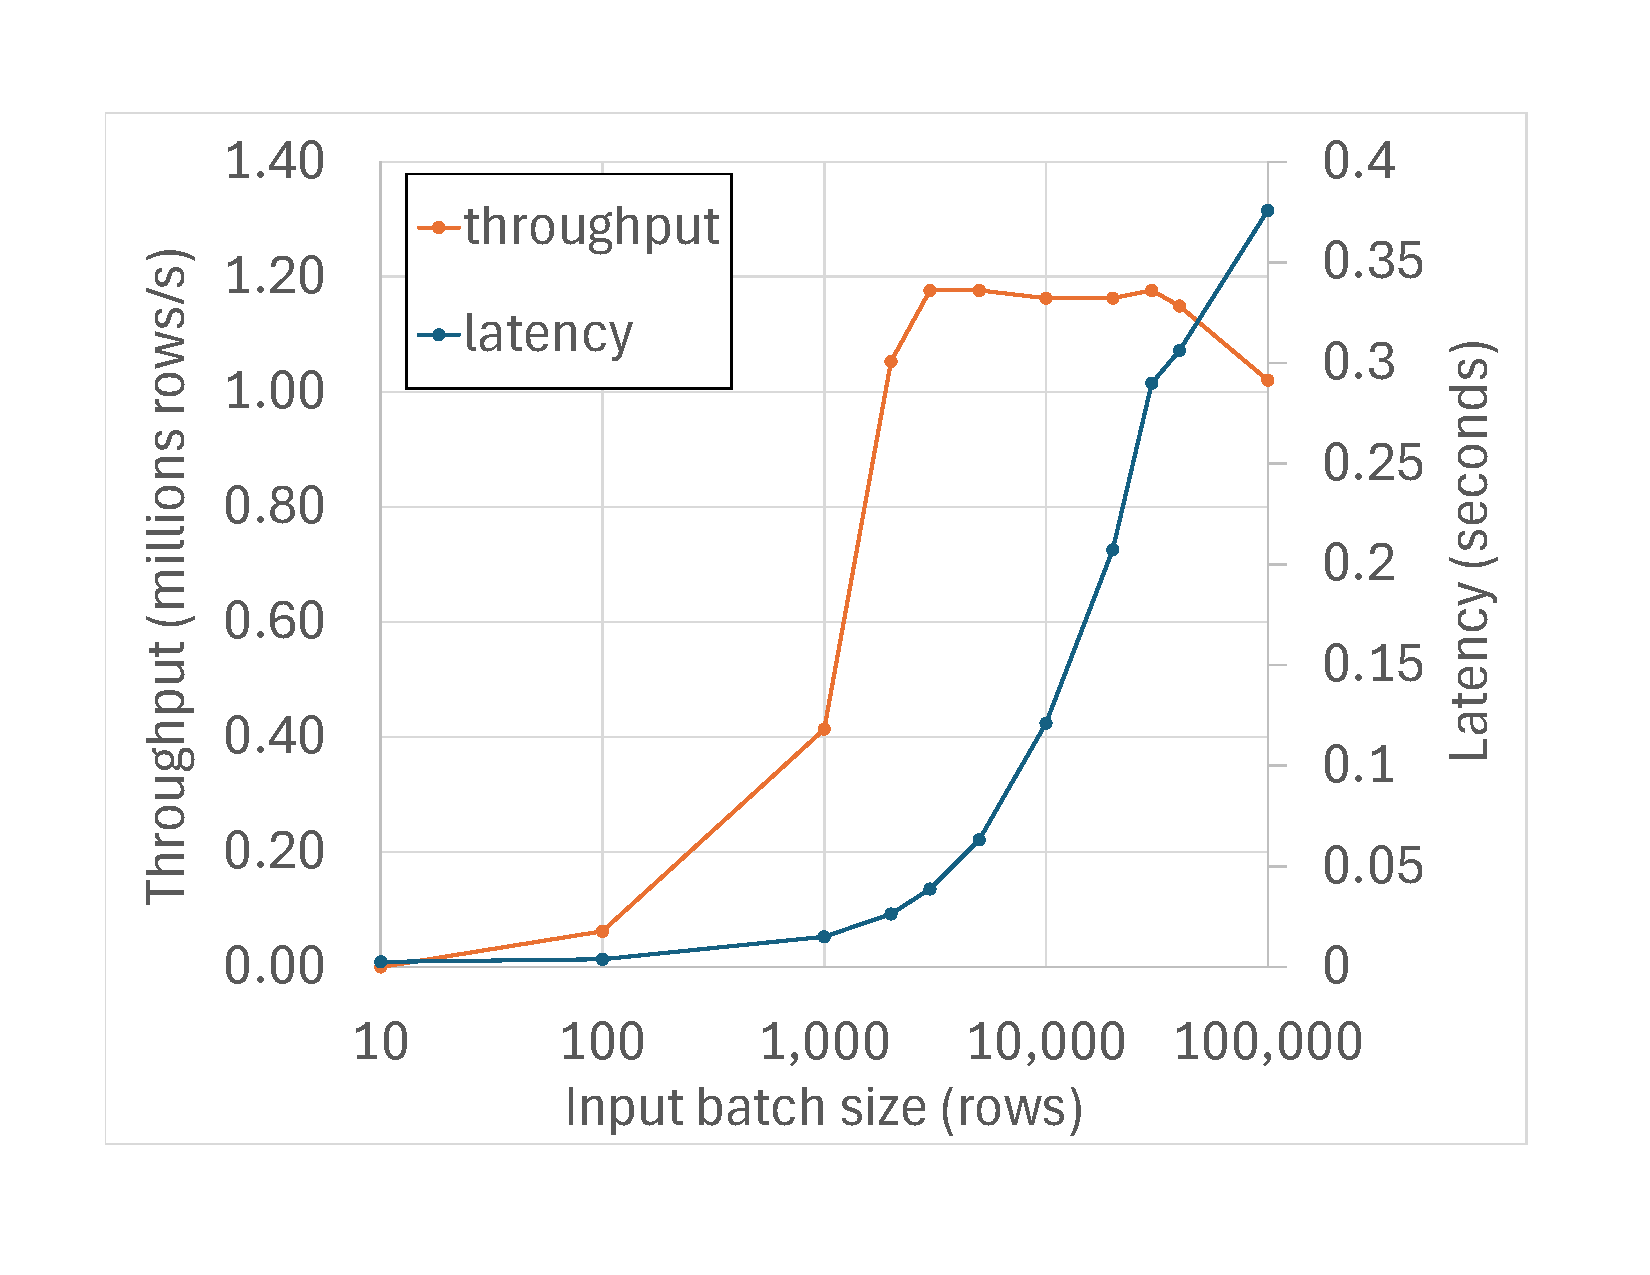
\includegraphics[width=.90\columnwidth]{graph/batchsize}
  \caption{Latency and throughput as a function of the input batch
    size.  Notice the logarithmic X axis.\label{fig:batchsize}}
\end{figure}

Increasing the batch size further beyond 100K records causes the
system to enter an unstable state (the crossover point depends on the
available memory size), in which throughput oscillates, as shown in
Figure~\ref{fig:oscillation}.  One reason this happens is that some
activities, such as merging batches, and garbage collection of useless
records, only happen between circuit steps.  The right solution to
smooth these oscillations is probably a dynamic controller for input
sizes, but also for partitioning resources like memory between \dbsp
operators and their shards.

\begin{figure}[h]
  \begin{center}
  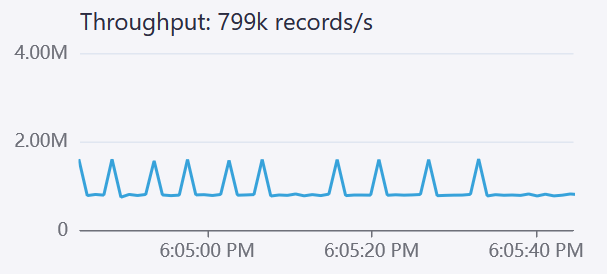
\includegraphics[scale=.5]{graph/oscillation}
  \caption{Unstable throughput for very large input batch
    sizes\label{fig:oscillation}.}
  \end{center}
\end{figure}

\subsection{Macrobenchmarks}\label{sec:macrobenchmarks}

\begin{figure*}
  (a) 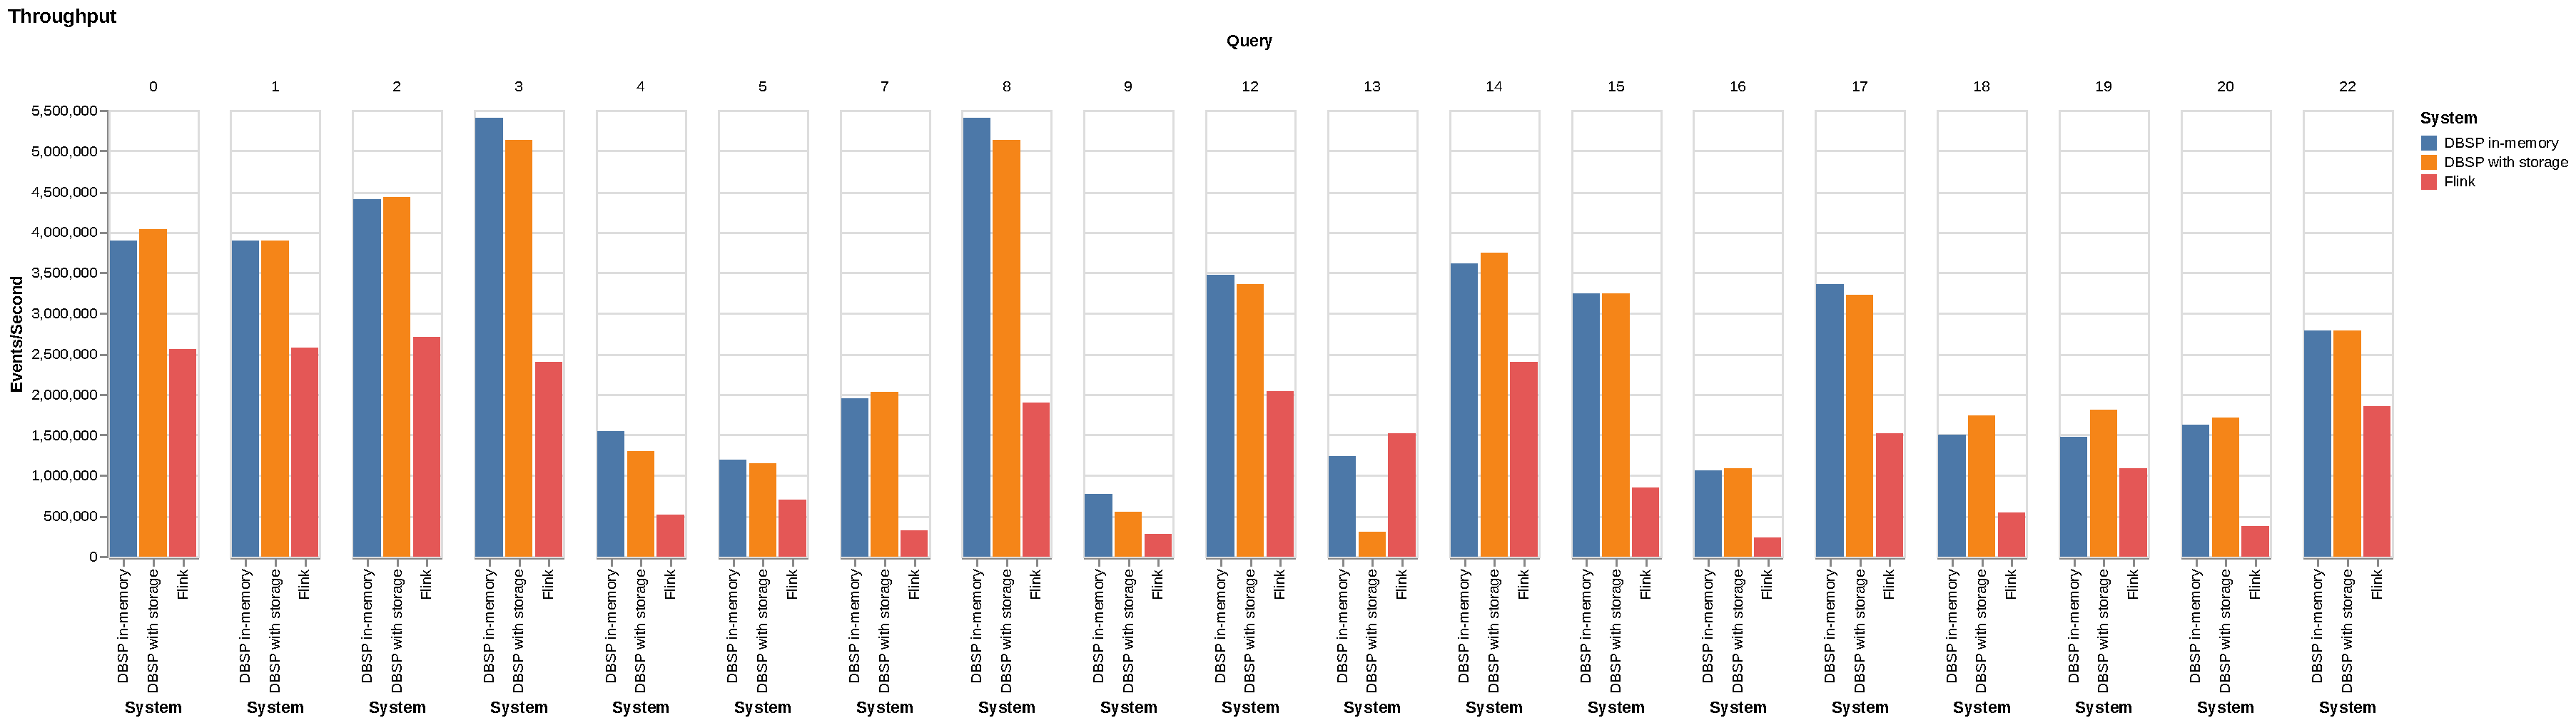
\includegraphics[width=.95\textwidth]{graph/throughput} \\
  (b) 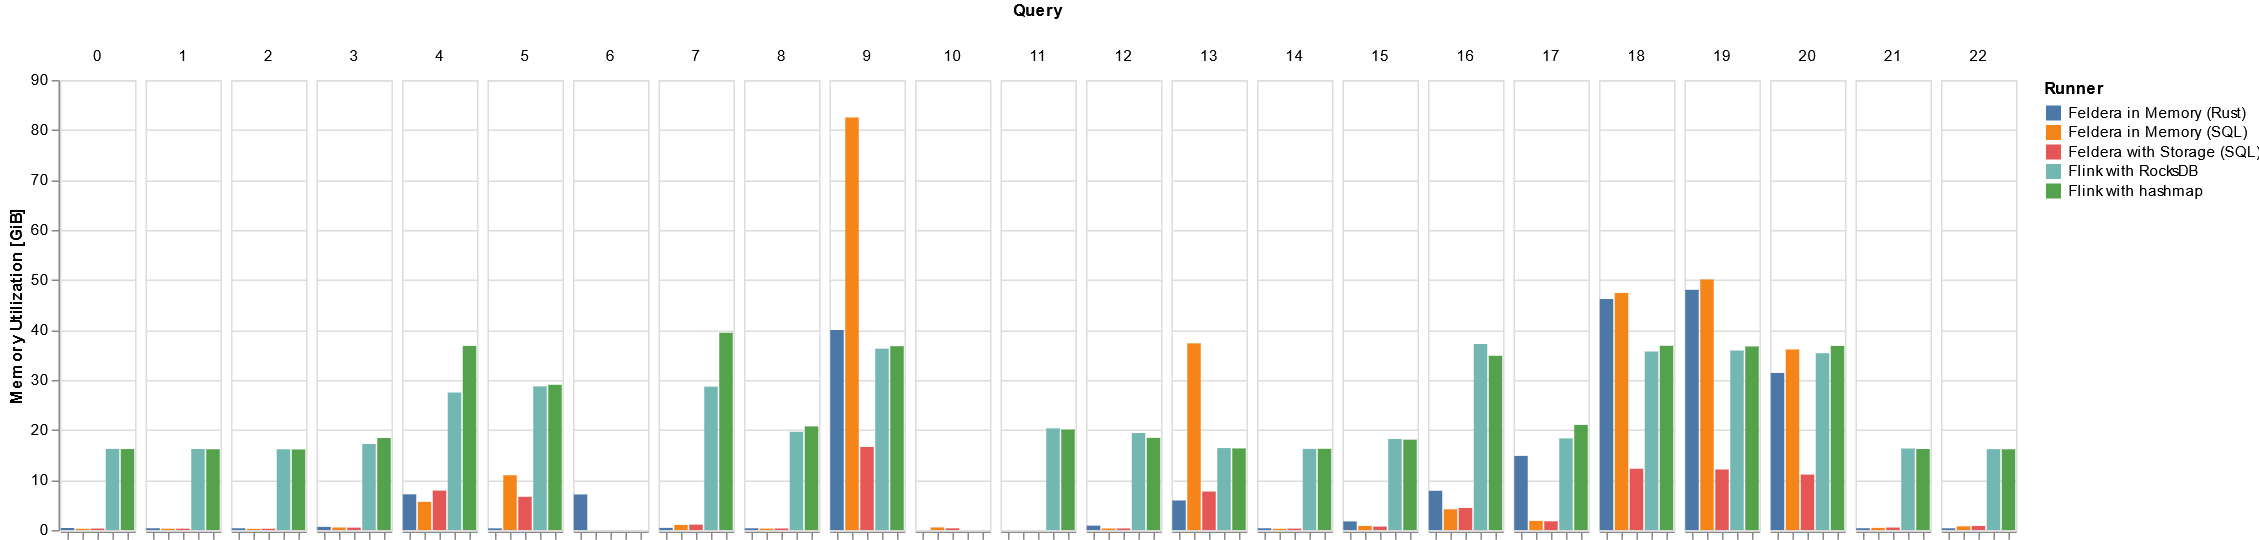
\includegraphics[width=.95\textwidth]{graph/memory} \\
  \caption{(a) Average throughput, in events processed per second
    (higher is better), and (b) peak memory consumption (lower is
    better), in GiB (\(2^{30}\) bytes).  The workload comprises the
    Nexmark queries that DBSP and Flink support in common, over
    100,000,000 events.\label{fig:macrobenchmark}}
\end{figure*}

There are no standard benchmark suites for IVM.  In this section we
use an atypical benchmark suite, Nexmark~\cite{tucker2008nexmark},
which was designed for benchmarking streaming systems.  The benchmark
is driven by a synthetic data generator, modeling an online
auction site along with a suite of queries against the streams.
Nexmark is already implemented for other streaming database systems,
notably for Flink~\cite{carbone-ieee15,nexmark-flink}, a widely used
stream processing system.  Nexmark is an unusual benchmark, since the
data is append-only, and thus grows unbounded.  The required internal
state would also grow unbounded if the input is assumed to be
arbitrary.  However, given some weak assumptions about the ordering of
the inputs, these queries \emph{can} be implemented using finite state
using a garbage-collection mechanism that deletes internal state which
cannot influence any future outputs.  We leave this subject for a
future paper.  This kind of benchmarks can only be implemented using a
\dbsp-like model of computation, where the output is a stream of
changes (and not the full views, which would also grow unbounded).

We compare \dbsp against Flink on the Nexmark benchmark, which
consists of 23 queries.  We use the queries that the Flink and \dbsp
implementations have in common.  We omitted \query{q6} because there
was no Flink implementation, and \query{q10} because we could not make
Flink's implementation for it work.  We omitted \query{q11} and
\query{q21} because DBSP does not yet fully support session windows
and user-defined Rust functions.\footnote{The latter feature is
expected to be ready soon.}

We ran both the Flink and \dbsp implementations on the same machine,
which has a 64-core, 128-thread Threadripper~3990X CPU and 256~GB RAM,
with Fedora Core~40 as the operating system. We present results for
100~million Nexmark events (input records), which is a moderate
number.

\dbsp runs as a single process with 16~worker threads, and otherwise
with default settings.  We ran \dbsp both with storage disabled, where
\dbsp keeps all state in RAM, and with storage enabled, where \dbsp
flushes large batches to secondary storage
(see~\ref{sec:state-management}).  Enabling storage allows \dbsp to
work with more state with less memory use, at some cost in throughput.

We configured the Flink implementation of Nexmark with the settings
recommended by the upstream project, running 8~Flink task manager
containers, each allocated 2~cores, and one Flink job manager
container.  We tried adjusting Flink and Nexmark settings, but none of
these changes improved Flink performance in a significant and
reproducible way.

\dbsp and Flink support reading input from multiple kinds of data
sources.  For these measurements, we configured both of them to use
their own integrated Nexmark event generators, rather than pulling
them from Kafka or HTTP or another source.  This eliminated network
service performance and configuration as a possible source of
variability.

Figure~\ref{fig:macrobenchmark} reports our measurements.  The two
bars for \dbsp in each case report results with and without enabling
secondary storage.

\paragraph{Throughput.}

\newcommand{\x}{\(\times\)}

Figure~\ref{fig:macrobenchmark}(a) shows throughput of \dbsp versus
Flink.  With storage disabled, DBSP is up to 6.2\x{} faster than Flink, with a
geometric mean of 2.2\x{} faster on average.  As queries get more
complicated, \dbsp's advantage over Flink grows by a much larger
factor.  For example, \query{q7} is 6.2\x{} faster in \dbsp vs. Flink,
and q16 and q20 are about 4.5\x{} faster.

\query{q13} is an outlier that performs slightly slower in our system
than Flink; with storage enabled, it is slower than Flink.  We are
investigating this behavior.  With \query{q13} excluded, every
remaining query runs at least 1.4\x{} faster in Feldera (with or
without storage).

Storage generally has a small impact on our throughput, except for
\query{q13}, where it has about a 4\x{} penalty.  \query{q0} and other
very simple queries are about 1.5\x{} faster.

\paragraph{Peak memory.}

Figure~\ref{fig:macrobenchmark}(b) shows peak memory consumption, as
reported as the operating system resident set size (RSS), for the
Flink or DBSP processes.  In our case this is a single process; for
Flink, it is the sum of the RSS in the 8 task manager containers.  We
did not include the control plane in either case (in Feldera's system,
the pipeline manager; in Flink, the job manager).

DBSP uses between 0.03\x{} and 2.6\x{} as much memory of Flink, with a
geometric mean of 0.24\x{}.

\query{q0} and several other queries use 2~GiB or less memory with our
implementation, but over 17~GiB with Flink.  These queries are linear,
and do not require any state, or only minimal state, so it does not
allocate much memory.  Flink runs under the Java Virtual Machine,
which might cause it to allocate a high minimum amount of memory.

Most queries use less memory in our system than in Flink.  \query{q9}
and \query{q13} use substantially more, and \query{q18} and
\query{q19} use somewhat more, and storage reduces the storage
significantly.

\section{Related work}\label{sec:related}

Incremental view
maintenance~\cite{gupta-sigmod93,griffin-sigmod95,chaudhuri-icde95,gupta-idb95,chirkova-book12}
is a much studied problem in databases.  A survey of results for
Datalog queries is present in~\cite{motik-ai19}.  The standard
approach is as follows: given a query $Q$, discover a ``delta query'',
a ``differential'' version $\Delta Q$ that satisfies the equation:
$Q(d+\Delta d)=Q(d)+\Delta Q(d,\Delta d)$, and which can be used to
compute the change for a new input reusing the previous output.
DBToaster introduced recursive recursive
IVM~\cite{ahmad-vldb09,koch-pods10}, where the incrementalization
process is repeated for the delta query.

\dbsp is an ``eager'' or ``top-down'' execution model: it constantly
maintains the entire contents of any number of views, even if no one
really wants to inspect the views.  In contrast, ``lazy'' or
``bottom-up'' models only build part of the views when the views are
inspected.  Such models have the potential to be more efficient.
Eager models can be converted into lazy ones if something is known
about the class of operations that will be executed against the views.

\cite{bengoli-sigmod19} proposes using SQL to express both standard
database queries and streaming queries and provides an implementation
for RedShift.  While this is a very nice goal, the \dbsp theory allows
us to formally argue that there are many classes of queries that
cannot be expressed in SQL.  So the question becomes perhaps ``what
are the minimal changes that should be made to SQL to enable enabling
stream processing?''

Many custom algorithms were published for various classes of queries:
e.g.~\cite{koch-pods16} handles positive nested relational calculus.
DYN~\cite{idris-sigmod17,idris-vldb18}~\cite{idris-sigmod19} focus on acyclic
conjunctive queries.  Instead of keeping the output view materialized
they build data structures that allow efficiently querying the output
views.  PAI maps~\cite{abeysinghe-sigmod22} are specially designed for
queries with correlated aggregations.  AJU~\cite{wang-sigmod20}
focuses on foreign-key joins.  It is a matter of future work to
evaluate whether custom \dbsp operators can match the efficiency of
systems specialized for narrow classes of queries.

\dbsp is a bottom-up system, which always produces eagerly
the \emph{changes} to the output views.
Instead of maintaining the output view entirely, \dbsp proposes
generating deltas as the output of the computation (similar to the kSQL~\cite{jafarpour-edbt19}
\texttt{EMIT CHANGES} queries).  The idea that both
inputs and outputs to an IVM system are streams of changes
seems trivial, but this is key to the symmetry of our solution:
both in our definition of IVM~(\ref{def:inc}), and the fundamental
reason that the chain rule exists --- the chain rule is the one that makes our
structural induction IVM algorithm possible.

Several IVM algorithms for Datalog-like languages use counting based
approaches~\cite{Dewan-iis92,motik-aaai15} that maintain the number of
derivations of each output fact: DRed~\cite{gupta-sigmod93} and its
variants~\cite{Ceri-VLDB91,Wolfson-sigmod91,Staudt-vldb96,Kotowski-rr11,Lu-sigmod95,Apt-sigmod87},
the backward-forward algorithm and
variants~\cite{motik-aaai15,Harrison-wdd92,motik-ai19}.  \dbsp is more
general, and our incrementalization algorithm handles arbitrary
recursive queries and generates more efficient plans for recursive
queries in the presence of arbitrary updates (especially deletions,
where competing approaches may over-delete).  Interestingly, the \zrs
weights in \dbsp are related to the counting-number-of-derivations
approaches, but our use of the $\distinct$ operator shows that precise
counting is not necessary.

Picallo et al.~\cite{picallo-scop19} provide a general solution to IVM for
rich languages.  \dbsp requires a group structure on the values operated on;
this assumption has two major practical benefits: it simplifies the mathematics considerably
(e.g., Picallo uses monoid actions to model changes), and it provides a general, simple
algorithm (\ref{algorithm-inc}) for incrementalizing arbitrary programs.  The downside of
\dbsp is that one has to find a suitable group structure (e.g., \zrs for sets) to ``embed''
the computation.  Picallo's notion of ``derivative'' is not unique: they need creativity to choose
the right derivative definition, we need creativity to find the right group structure.

Finding a suitable group structure has proven easy for relations (both~\cite{koch-pods10}
and~\cite{green-tcs11} use \zrs to uniformly model data and insertions/deletions), but it is
not obvious how to do it for other data types, such as sorted collections, or tree-shaped
collections (e.g., XML or JSON documents)~\cite{foster-planx08}.  An intriguing question
is ``what other interesting group structures could this be applied to besides \zrs?''
Papers such as~\cite{nikolic-icmd18} explore other possibilities, such as matrix algebra,
linear ML models, or conjunctive queries.

\dbsp does not do anything special for triangle queries~\cite{kara-tds20}.  Are there
better algorithms for this case?

\dbsp can also model window and stream database
queries~\cite{arasu-tr02,aurora}; it is an interesting question
whether there are CQL queries that cannot be expressed in \dbsp (we
conjecture that there aren't any).

\cite{bonifati-iclp2018} implemented a verified IVM algorithm for a particular
class of graph queries called Regular Datalog, with an implementation machine-checked in the
Coq proof assistant. Their focus is on a particular algorithm and the approach does not
consider other SQL operators, general recursion, or custom operators (although it is modular
in the sense that it works on any query by incrementalizing it recursively). Furthermore,
for all queries a deletion in the input change stream requires running the non-incremental
query to recover.  We formally verify the theorems in our paper, which
are much broader in scope, but not our implementations.

\cite{svingos-amd23} uses foreign key information to optimize query
plan generation.  These techniques are only sound in the absence of
updates, so we use them for streaming-only queries.

\dbsp is also related to Differential Dataflow (DD)~\cite{mcsherry-cidr13,murray-sosp13}
and its theoretical foundations~\cite{abadi-fossacs15} (and recently~\cite{mcsherry-vldb20,chothia-vldb16}).
DD's computational model is more powerful than
\dbsp, since it allows time values to be part of an arbitrary lattice.
In fact, DD is the only other framework which we are aware of that can incrementalize
recursive queries as efficiently as \dbsp does.
In contrast, our model uses either ``linear'' times, or nested time dimensions via the modular lifting transformer ($\lift{}$).
\dbsp can express both
incremental and non-incremental computations.  Most importantly, \dbsp comes with Algorithm~\ref{algorithm-inc}, a syntax-directed translation that can convert
any expressible query into an incremental version --- in DD users have
to assemble incremental queries manually using incremental operators.
(materialize.com offers a product that automates incrementalization
for SQL queries based on DD.  Differential Datalog~\cite{ryzhyk-datalog19}
does it for a Datalog dialect.)  Unlike DD, \dbsp is a modular theory,
which easily accommodates the addition of new operators:  as long as we can
express a new operator as a \dbsp circuit, we can (1) define its incremental version,
(2) apply the incrementalization algorithm to obtain an efficient
incremental implementation, and (3) be confident that it composes with any
other operators.

\cite{akidau-amd23,akidau-debs24} describe the Snowflake incremental
and streaming capabilities.


\section{Conclusions}\label{sec:conclusions}%\label{sec:ddlog}

We have introduced \dbsp, a model of computation based on infinite
streams over abelian groups.  In this model streams are used for 3
purposes: (1) to model consecutive snapshots of a database, (2) to
model consecutive changes (deltas, or transactions) applied to a
database and changes of a maintained view, (3) to model consecutive
values of loop-carried variables in recursive computations.

We have defined an abstract notion of incremental computation over
streams, and defined the incrementalization operator $\inc{\cdot}$,
which transforms an \emph{arbitrary} stream computation $Q$ into its
incremental version $\inc{Q}$.  The incrementalization operator has
some very nice algebraic properties, which gave us a general algorithm
for incrementalizing many classes of complex queries, including
arbitrary recursive queries.

We believe that \dbsp can form a solid foundation for a theory and practice of
streaming incremental computation.


\bibliographystyle{plain}
\bibliography{main}

%\appendix
%%PDF-1.5
%����
1 0 obj
<<
/Length 843       
/Filter /FlateDecode
>>
stream
x�mUMo�0��Wx���N�W����H��
Z�&��T���~3ڮ�z��y�87?�����n�k��N�ehܤ��=77U�\�;?:׺v�==��o��n�U����;O^u���u#���½��O
��ۍ�=٘�a�?���kLy�6F��/7��}��̽���][�H<Si��c�ݾk�^�90�j��YV����H^����v}0����<���rL���
��ͯ�_�/��Ck���B�n��y���W������THk����u��qö{s�\녚��"p]�Ϟќ��K�յ�u�/��A�	)`JbD>`���2���$`�TY'`�(Zq����BJŌ
)K�̌%553<�,��(�h�l��wB�6��0��a�G�+L�gı�c�W�	c�rn
�q��9�����Mܗ8%����CMq.�5�S�hr����A���I���皎��\S���ȩ����]8�`Y�7ь1O�ye���zl��,dmYĸ�S�SJf�-�1i�:C&e	c4�R�������$D&��
�&+ü�bL���a�j� ��b��y�����+��b��YB��������g�	�YJ�Y�Yr֟b����x(r����GT��̛��`F+�٭L,C9���?d+�����͊���1��1���ӊ��Ċ��׊�T_��~+�Cg!��o!��_����?��?�����/�?㫄���Y
���?^�B����\�j�UP���{���xᇻL��^U}9pQ��q����0�O}c���}����3t�Ȣ}�Ə!VOu���˷
endstream
endobj
5 0 obj
<<
/Length 586       
/Filter /FlateDecode
>>
stream
x�mTˎ�0��+�$���$0�� �����
�a#A%��߯����jD�岻��f��c;Z����̫����MfG��}�
q�]/��ޭ�mޯ�o⣩����0Z���^�x]f�kn{��E+{*ʧy�pg�6;5�P���V��pH8$h��mڢ*߄z�R:")󨺠���3�q��X�ysO'H�)-�"��}������[��˺<V^��[l��Fռx�M�ۦ(Ob��q��Z�g��Bz������<��/V���[m��XqY�۶�g�ٗ'�R.D�ϖ�?k3�q8~�J�����#��K"�3Gh��AH
��9lVL@aR��L8��DB��^�#A@�J��0�:�p�T�
�K�Ⱦ��Ͼqi.��a��0N��\�����p��g���\���8z�s��3�'_��&��A���5U�X��)� W`�#Ґç�v/�L0���^��Eɘ4��^ySS�W�+%={�H��}Q��jŷ��������1|>s	��3
4�{��p�Y�d�r���K�+���� a}����ѫ�W���{Fvm734�4�����A����G��c ڤ�_86
endstream
endobj
6 0 obj
<<
/Length 770       
/Filter /FlateDecode
>>
stream
x�mU�n�0���E��"��y$U�6�ɢ5�h�)8�"�,���c\W��s�/.7?��3��oz��(yѧ�2�z�v������Aw�G�݌��=y�z���Vm�Mמ�MW\=j�_I����*�Cn_����f�
����&1y�+���S�w�$���F�5�? �S4��!�1�����!r3Ҵ����>�Za��<��a���h�"�#<��O���h�44zh�wr��1p{9?4B�4Z�I��Ƌ��qw�d>�?�ɻ�=���ñK��}:�j=�w�(]�UU�#�5�d�k�u�ѥ�y�e���*��x12+��Sx��,���09�9�)5t�J��N��'����{fS�
�2��R�̼	�K���Vi�X���B�Rs>�^��
�.��K�Cc��2����c4�&W��o"������q��8^zl�	�p5u%�=c�K(�q/�?�x�Q��c�c��/�s/G|������-m������ƯP/S8+8���4f�R�SYZ"?.�0�1�шŕ[K����������PKS6��0���e�;U��}Z8~S�g�;�
_����g�v��i;K����c��g��̭oZ�����	����'���L��^
���^�$�K��{)�p/E�X�{)��^
�(½ߎ��<Fߥ��*����p�V��{-Uxbd�1��2�6��ԗޢ�*�Z}��9+�B%Ӝ�����g���e�)��{�q��NO��c��}�g��=U�?*�a
endstream
endobj
137 0 obj
<<
/Length 5923      
/Filter /FlateDecode
>>
stream
xڽ<�r㶒��ڗ-�ֆ�	r��*sI�f+�\�'g��y�e�b�D9"���ۍn�Eٓ<�@�F���T��[d��~�M~__���F�|!�P27���EnD��EQB�|qu��e����^�]�<[�:�fyv�zhW���[���e�m���P��msf���Ỻ톦��UC��=5~jWkj��颁^�/�>]��B�LȢX\�JT������]���XH)�<W:LV"Szq�
���|׮�6y}�i�TX�P��Y�����[������ڝ�Am��=��E)���)M�^�_=l�L�-�j���V�65�E%%-puV�e���f]�����,Ȁ�Wf�M
�
�|)�6@!1�����_|٫�f���R�@q	���C�o�M�gHJ�*ʜ�yՏ[|��&?��RV��`��E�����Q�����_��D.u
�s����'d�a�q�/�8�	�>+��綫3S-�k�Y���R����kp�}�����~h���<�][�SH-��x�7_�Q{q�G��A$��H�Dy���2�2R��U%qwɫ�z���''`�\�>+
'�`~�aAXj�ka��U8)W[�,���aD�r�
"R'��anڒz�uO�7��Z�piٲ��Ҩ�ެ`�=�/��g�rw}AxY4�V�aE�n�-L��e���M=����\�
uk"N�Ly��滺{�V���v�!ĕ��
=L���������]��ōE��@�j�2�Cn?�����������GE�K�q'���������܇V���Y��6��x&�U�9�P���H﮹���tN�`��-����9�U˫up�N�Zw��;^��~����z8��n�wM��I� 8@��U(�R<.��%�k�8��FDz����a���s_K���.jyG,K�5�H�Թn���|q�R	iau�� 4�ꩈh�����l�`��d-��]j���Imd)ɼT�?���W����=5Oo��O���#�k
q��"r��D���0��	�h�ђ�ql����X�,A
���3���^$-OᲨ��r�)����Wo���čbܔe�
��xz�%%�n�����4`2��k��z0��v
����غCĠ*��'���������#a@-�.x��c��urE�Y>R#Z$�Nq�1`����z�sb�`hA" "5#�="�ٯw�5x�95�mw��
?�$E�C�(�Ų�X�|���9W����T*������ɧ�B�v�
��%�?h�6jM!t��xOXK���rҌÈ�����5�Qhl����s��u�t �'�ś���PN4w�����F��F���(��fn��{N��d��V��D����.&�P��`���A\72b��x��2
��@��<�x�3C�(;H��^~lY9~�Dy���7xRA�~�6h�	�&S�ks��=����w�:~l���Z4�F��I��r@��˫3��=u׼>���C
=6C$�Ma���7�'ꐡv�A�Y�=�S�
�F�
R�
�P=
F�w��ų�g�~��tc�_46��m2L������3g3g�j]����o߾�n�m�N�ov{�/G#7Z�X�i#���YM��9��s4�9��s��?өƯS'H��/���!��Б�!fQ��О���?��A���?���`'��9u��ENd8?~�xc.��Ǩ�/�8�2h���7���Ǐ���ˏ�����1f	��~ho���qT��a����݀{6K&�sv�y�(��*o]��B�P({�Y��#�
�����!�A~4ܬ>f3t2�:N��0��t����a�V����0%//�g�����(_z�|qvQ����G�v����,��#n��O�
%E!9@$����m�W?}��o��}�~�=�
���K�)1�]0�0��T��[����b/�8E�{F�w�j�����8�a	U�>�[�Eq?��E��[��ܲC�����/�ŁI�K�|
��
�,�a�X��B�����RS�����(�������Ϳ�8��9+`ٳ�{�f4����*�~�<ye�m@���h�*�\�%P}
(��\��$'5x�:����
�8��y�f���1��D֞�
�P��d3��O0Td�X4�4�끤Gˡ��o݊��w(|!2⽠˗�h�O�k�zc��&����4bӉ���[�"x�?�-��lr~UV�-��<�!�dE��y��z�ʀ]i����^���bs�"4��'�&�L�9G��L7���{y�U
ͦ�O�n�Tf���d��[ #��Y\P$��,��-d�+��H�y�Aix�p��;
�̻�?W�����\"]:A-�MeNQ~Ek,W`����}�J�=Eey�wȬx�̊/ 3�#����M�u1�ݖ0��VkAO�<�өc!���N�hX0�Ljt�܈�y�BP�rʫ�aJg��ğ�}�~]� ę	h���u<0V�w�e�w���DA�}P�2���7��w���
x����I�,����m��w��w�8=�1%�oѝ���cf���^�Z����/']�e�]/��8�P�Y�(E�W��d���Q��f��L��z�����,
������/���
�C9���g7r�0V�
�m^��3�Ţ�~�K쪪���^0l�^q�9sF�n�9<߹iWM7�	����4��s��L�a��B�n���i�|���,^�s��-��y�oh��r9���\����P`�̻�}�Β�V ,�b���]�A���Gp�\v+�UK�w�K>ю~b�f��Cߘ*cGp�rXO�6���wX)؈x�om��pݍG�ΏXEҦ\Ɨq���l��.���¶�{��h
���	��B���l�
��1Rr������!'
�,��;L�ۻ���Ӻٸ�]A�E	"�k�����G���|p���5��n�~Σ�YI��="b�a�����q���&�/��ȿ$u��^�4����|7?��0e#|����"ұ�'>��88�eV���BG��(){dby�M+�Ҫ9�B>��/r��b��u7A�Oq�!�Xt�SZ�(�e�����4�G]-�KS�En�q��$V��o��A@�~�n� \�O38���E�䑠����0j+��
�x��y���M�dƇ߷�]K1�R.?�w�(�?$qǻ4Rw>[�(�c�]p�A��>�ӊ���c�fz^U���g`�c݄�np�z��gr�1jx��D"�"g뵻�E��a��i��`J���?�3)��w�%��#bU>;�����
~���j���2��!V���O9HGS�������J/r�J�I����ٯȃb&���kFm���{�(#]h���W�ssL���~ ��}P�f�x+z
:^���j�>��()`��X�Jp�u�t�k��>�۠�:��9�3�U��h�b��s��S���ˣ�*��-����'��e�ƃI��\�b)oˑbq��IP-8���[%�Z)��`���l�s�n˃|��i�[+����O���pev
XA��uF4�0����j��nZ��v	$�K���H'���
��.��z����`�6W��{p��"��<s5H��H����fq45Fl�x[�+lFM4D�_�fCC�O�	�
�^:u}�D�+�2,M�ƨ���}�J����{�X"��7ʹJ7�H&SO-�oK��o�䌃-G�~L�Q��S&өs%&'BS�*��d.��6m��\������J�b�����Ϧ��x��!
VI��#wye|�*C!d�j�7 A��M;`Y�3=��c�ؤd�q�~��^L� Y!d�j($U�*�P���򚑨0VTJ�2h��)E�)e���SQ�k���r�d�jy�/ذq�s
��r��o���
�o�i����W�U
�\��,���]���\��
�Q���Y�1�<^��)r0:-�0se&-��ib��v����b
��B{�fA\��T&��TG�6
C
����4GE���q���-�`'q����H���)�C�s���svؘ�:��Y���;]�~���D0�SX��.�`�+A��f�C\�!�bV��w>s�5Q)<\���;�3����m�L���z�܏�d�M3���$U��<�Ui[RP�I�
�����"�"'
E�J�(�
�f��l��!a��Eo��b,�!��5���5�{�w�a��5�␌�M�"2�7��*K�K��E6TKT�| _&i�#C�{bc:�U�G��B�������_r����3+���$�<>y�e%,x���Q����[�@.��I�W��A��C��E
��3����8B/�����e��ZU�(2�԰V�>�Vf��������ǨM��ooÎ5^�`^�'s�@�姿w���;GKHO.]��(��؛��ϰw��t*��M�?�l���׳ڦ�Ͻ[��v7B��[��&:������-�x��3р�p@ދ�̧
�SXjkr(���h#�sT@�݅�ب�٨�o�@3q��X�W�T�Y|��1Uha��ɖIQs܂�]1MG����HV�,m}�S�:�>���^��X;���Ѷ
���4�W؂5�|�>E��D���UDAԭ�pYޙ�ޛ�4�����Ix_���J�9	�P9���"��b��Ɨ���z��;�䄽Q��1��l�������&��m9Q9c�M��x�z�������1P���vێ*�$J�&���WM�?��U��M�N+Qo��'�ߍ`B�N�XuSF%�a3�b�ե�܆z��|t��>roi�Լl�i��1[�0���h!�ep����nK̜F��}R��\���I-�v>v:��Â��ޤ�bN]�
S �z;-p>Om��c��8��Zn�~u��4���M1�k��YZ'ӣ�KW&��Fa[�M�[��ĭ�3�
�=����t��u��)�d���Lf�(2�L0
���a�3'�[���ɉVBA�,�z	x���<xY���r��NҢ�7�^xF���b@
�
���(��E�2�U�$�;H�~	�Z��P>�(�;�-�������/�eVU$���rU+�/^D[>����*O�=�����o{�i��}�d&���ړc����BTcM�����M_t��p�2���Ⱥ�Ϫ��.������|�%S�E��ь�:.��s�*8����-���e��3�,�,��gn�����_���5���Ao���i�b����
���
Ѐ��>�
�$TC�|2��s���餋�?)e�4ԅ>�&�[ Y��sD�IЉ���OU�]��-~i�n����#�L�^a?�.�����`H?�
��"�[�����M�eϛ�N*?yUFT�&�ߜR=�]�"�l:+|dD�t<��0bM�����*����a��w�Ϣ���K������.�Xf�~�,�0��^"���uq9#�%�9�9���{4i�Xg�U����>ډ/��E�
,�)��ʅ{V0ۡK���r��}�����_Et%(��I��T�H��QPS�(�Ѵz�J>;�T�����#.��O�&U%�a�/�C'5��/�1����^f�V��>q�����hOZ�J��|��Q���VkMy�5'e�Of��e��T�j���_�fU��Q:y~U0H�j��Ξ3ӬuE�1:8sA��BG�E�
�DY
]Nm�~�N:sE�_��<I��-�H�_���{�B��#5�����;�/�q��bw,=�qsΝ�)��UNѓB�z�`y9[���Ջ�R�U
endstream
endobj
175 0 obj
<<
/Length 9035      
/Filter /FlateDecode
>>
stream
x��=k�#����+��h�Q��f;^;.�%�;�C�fF�F������_��&[liv�$0��E�XoV���Y;��'�į��ۙ�	m��̵��L7�y��3(��Y(�IۨΛ��>��Xu�	5�������/��y�������v�p�h���ʛ����W��3�t�x���M׹Y,��v�����?�����J�jf�ǒ����:C�Z,��/�f#�>�.�0�DcJC�7���-|cZ�AC�C^?U�5���7B��9����K}a^c��W15�Y���ƔF.��+E#m+$�J�����)��(�g���7Cuj_�A]@���^9kN4J+��P�NM�k��8�P��oZs:���X6�w��
F7�ETh)��%۶1Z�d�������8**5�B>��X�V>(�w���M�*��f�p���c%x���'_��9��x��l��\5դ���xkT��Ǚl�T�D�I���_0M����,��Pbk��\����n��Y9P�[@�#��v��d�q��ɱ���h�i���;�l�/���0
v���E?���ߦ ڋ�(��}�-��Z�C�J�blq���Q��oaG}}��|y�����_������ͷ�f{G������t����Zp����%��U�ie��V�BP����q��ƽ�x�#q����h�����*ɖ����f��V�M��펞�.����q5~��w=�)�yC������\H�������*�jb����� �&6B�u�Q@�Xݫ����/p�iD�'�&�U�
ښQ�i%��0��fރ��7���a{�sS�!
lfc�j#!\?nq�a��&@[���̫�� �;s���a�-� ���^��M���A�rq�ᙦC�E�C^-�V�d�4�IGBG�%n��
��gC��
\�pa.̢���yM}��#=7N�ˆ�qH��x	$@Q�w��c�S�X��Ŕ@��`t�yX>��0oW�K��6�w�=��{�苛u���o����Y��������9p�[�b�o��
��	���/˞�֫@}nG����_��d�ã�V@��X�_x��x���z�Y�����w�4n�͟#|m7�+����i����~M�@�pG��LН��
dݢq�vz� ��.�F:U������vTc�f���6�P%�]p�<�@�\ ӈ�W�f,'X�f�9,7ƌr֍�H@���im:����X�a��\b���n�]�,<���У#�1�cl����_�
ߍ��'�~��n�r/������|:U%+ Z�@Qt�Mۊ��Ц٩aW1S�Ȥt(<��\�V<�@
&G�s�U�{VA*�2�XSֺy�7����bUЊZxZT�&���]�W�&�Em`���b�B���������d"Gx];����;���N���#��������.B�3a�:7�6%:�r	x�6,|��J�i�����
h��a10����kK8^f���5Em�!�DM�:�t�7ӊ4�_�:�����������O�V	(j��%]|��`��#�?(�H&Ρ%
�hJ���D�@_i���k�A��h�Q�=��#�e�(��j\O�$����nR$��-����L��������$���40��H�'�+rM�D�kf���"�����m�R$
��(�x�B���'a�� c�����v�W�H0��iA�Y
D^ Q<�3�Ӎe���x?���L �M�F��:�3HLq �}o�w��><�U0p������M�Q'2]�^�sE�\���=^]�M�	�m�Lk�V}��0�A>ov��t�F^��@��_\�OK����<NB�w�,oJ�V�j�����w��`{<<Ee��|>�����(��wH�����V��Zj��cI;����,ӿ��B2><���6m�3�~�"����BVm�g�0b��]Ɉ2���/:^��h��)�@��X��|�!��~�~����8�\7��L������}��`Q�.;�(��+WV"S���9>װg�#��R-&$O�a�:�~�����e������r�������l|N���Ȫ+{��"�FK�.+}z���4�ɲƿ\k?�K��6p)��U��.z��05KH�F��\���XC1�"þ����_ߝ�M�O����s��j�}�茯O};�%R���Q 
[�YX	|gd�жk��c>70�*�C4�M�W�r�ӥJ�jT�)R{K;�~�~&�P��8H� ��L��Z��e��ڒa�n~�?�A��K�.s�J�Ŕ�
��xX���I"SۅTek�р���U���,\uɦ�"��k����[�����F�92�j�rDǒ������
��{�c�l�AY����'����y3�2��9K:*:]B��Y��u�B7���n@�9��<����a=���EJ��h�I(K�s@�$�-mp
�<��7���Gm��F]�05[h�����e�m��Ԙ�ny�u�6
�&�:u���y/ilih��/@d�Z�����t�<��s�}�
��8w ��,J��+*��X*L˗�Hl,kkz��&h���t|/l�0�0w��P��X"h#t8���p}����v�QN�b��ڐ/��mk닍;ۄ��H���L�Q+̌h��bC�N�Y,��x6����|6�mm�њ�z��V[J��:��%��~��{�@�8�N�Bko��R�F�hM��ɰ���G�ƒ�6�6��`�R�`��kEZ{ӺN�LQ��pr%�rq0�a��Mpv0E��:0�e�E&t���$P\E���OA�R0�H�ߢ�����Uq7T����Q�z�|V9��*l��Oj��<���hDY��P���ٰ�BgB3�`��Q�# �r0;Q�"6ݾ,bc��H���j'���Z^YX��^	J�nU�b<�O/�`:`����%��k2�{�G{C��
h(�nS�K:�o����_��hUi�Gt�+6�����=#]�}s�M�q���&*W�\i9����
�.���MKnZE��Bb��h;"y��b��WwE����C<�?�T�s���:�I\�h��!�f��j�܈<��=P�|�`�(�Ϳ��/V^�]��x���ݻ�a�#�4@6ó���&3EԷ:�͔:��a.�P4��b[�9���M������cJ��D/��e&@wa��Q����bI�Ǎ�@��G�D��za�*S�R�\R7 ��Du���*̷�����x�_���ظ-׏k����:]0�F�b��o��"M��9���}�����_��]��##nQi������s����U �T��ٟe����P��&���Z!�@��q�$�X����rs�"dߋ��ڲO�����Z�!
�.�.�
�����û��|]l7�&�#}�:��=�0��~Z#�s�:q�ق�#���7�P?���V�e�qB��p�i_ 4�������m��ct�E��R.���T����Uh�= N��{�<�vm�h�*\��d,�5� \<q���
�+�KD
�A����j���)X^�k��}�b��A�F�?}\�1��6���Я�iO?��7��M�Հ��������3�����N=�}��g!7t���]�1���-`��#m%
,�9���
��k9l����%P�ʻ?XTE�Z�n��w�K3�v4��dWA�7i�0���n�a"'��>x�뢝���e��_�Q�4���'S4�&+����u���a��n�H�`�9��]��ݑ��R0pE�ԳW�}+e0qW쵲��a�5���-P?3�'G��=��
v��O�I�3u^�ל�N�1AͶ��E�Sj@g�ͅ�{�tw�u�Wx�.�؊����A�@}��_3z��x�,P���N:*x����0�8��3���2�a�2;38ƿ�
�!ˮ��zmϳ;h��UCMC���ƭ�ʉ��a�#;�qY�x����ׄ}	��o�G�j&�l�o3r9�R�1c,��v3�Q�C��OkH���r�.#�9#
���}@$�6'Ѝ�Az���R��\�IQM�ǥ������t��h�d�#��$>��m��E�z�����
b��f���	�'�3�$,�_��m�����W�x�k}���02�M�[5��b��R?���z�:�zy�?�˫���^9y�
�b��M����`#*4��妆�N\�j�@�O�q�4���-,�i�q')����`a�3�����1�ڡA힚�@X9���L���Ax����D@�e���J�OV�g����;�-�]�_���7�*�rb
m��oyˉn�]�����M�V��R�#k8��&eP0��񐔛��[��X�,эU��xŸ�Ǭ�‰�c�C�� F�ܳc�}<C)�Q���=J�J���( 2F-�/s"T���ƅrv����͚͑�_$�9]�Z�2-T'0

Э����ǺT��Jᠬzm���=/T��k^��M��T��(n!]0�L@kWJ[��z�ԥ�������'�r�I�ug��JfK���Z�a�!Pq�[�{�C��-Q*{h(�g����w����EdI	p�
�F�,�w1��-:F�p���r�8Xf�jѕ`u�!�@�]
�A��aZ�hRf�!G���Q��xM�dO~u^gK���K��R�2�4)F�������m����{z����8�;	��
ҼF��=�
oc�zZZ��	��~[f�,t���M&��8����8/��H7򥀌BR�'���̨�qB�gH�?��dB%�ON�����&�o�'h����1:k+x+,����i�op~��\�3@]<�Ol�n`�o���}q��.@`��S:�C�j������f����В�qI���~}�|���C�
����"[6D�:��W���i�*��$��z(A�|���8��gFc��0�B2f����OF��dQ͚-TZ���1���ߗ����'r�����/SWY��gL��(�i�|C���P���9Q�`����~��'�%���.&I
N��h�D���t����G�H]��j�l5N*3�B�'�U�I`�>�G�D��O�g;���e�SVB	xjG�8���WX�����'�,�P�N��-�m'.�(�e=|����̀���_�E��T��Q��%Yd%'�&��%���:`d����5���j.�=6=��S~dc"�0Y*��
K�k{�,����^|[f5��6�Se�w��x����}p�5]Jk9�v@���L�ӕGٸ�x�8�����P��X�hU�ăh�o��oS��)S�DL�D�A�#�w��@�۰P��~`0�a���n�r�ؿ{.�(��7J��N�mA1J��^�����/&�,��yj�Q�%x
@�0��/5G�je`?��@�}��"
���_ �����,��q�ρ!V,Cr��DȒ2�J����H�XT�:��m .�03�]`:�l3���~i&�9�A:K�n<tr��GӅj+��x��5t��]���yrV�B|��9TI�K�8J���y�/�)�#G�$����0�8�$�O���z7��$�<̒�"L��xν+�
eJM�
�xϴ8����y|�)�,�&Gc�=�in���MX�M:ۺ1�3��_1�$	nt�֭��f�/�KK�oL��u&m�4����
�B1aJP�$\8��̚���m7��v�څ26ӈ�@ �
/0��z{O7ğ�4��@+5�u��I�;7<L\
L�)�eql<N�5�#nn����,��ę��6���,ۮ��L%������h_LӰ�NȄ�U1�L�ƀX�N��1�S0�5�̯"�
Jr�ӝ2A�<
�I�{���85�Ӓ�0>��%���Lެ��c�GL��NDo�Ñ)�va)4\D�η�=.(��(�-F�%��eH�#�M�5N23�縇Iy\]��y�Őd<KDiR&�8�l�no~R&WL�yP��,Եv���-��2�z�]�$�aL��S�d8��\�\�[fd��9l"�Lx���c�s3�w�w��H�q�j xs�=nn�-�B���~���9����n�~�!6���v>�GIo��џ��ј��e�B���
��e�?7���W�Rm�5��]�	Ɛu�^�J"�4ϒw�υ9��	��2�a�?�1x9_����%c-�OB���w)SY/W��>�.YYx�oV�h3�����n��Ѵ����Jow�YxZM�.�Ԛ�1��x��M��q��ӿ�: ���e���Jy��6������>F`Rl�(��z���ń*E�x&@�
dUOBD���G��I�0�@�/m�x]���ƪ�]���\a*45��)��FU�Q�Tw�4U��64�\�lS��[.�e;k������w�;��Q����f�U#�o�D �)]eR2���@]�i�
�*�Y�<��Y�=������VsnoVO��	�n+N�D�k�n.�4�ѳ
�I'�)/bg\O%v��b��٦�C�������ɋ�B�R��W���ө]�!+��	S�$p�fz�K6o
uOӃY�Φ��z}$9>��H�I��h	W�J���d7��ߡC7��+��T>���8��
_����#M5�"�5�O�p�H�sM�������|���&T�1��6��'zLXMRW^������d||��`�G�mН�g�IV�ö/��a1Z��qP�E�x��R�sӄ�DKV�擁������p,�� ߰�;�W@���<b:�t�������'w�t�e���q�__n�W�e�������] �w(��tʧ��m�_���/?�-U�����ac�7h�n��
.?��j�������2�xQN�RN�V2�!��6i�Hb�'\u,�������Cs���9��L���) �D�P�����r�ФC9��'J�
\Φ-
B�%:���4�h���T�q��敖�F*v���;+�&?�º��4�@N��0��F�H<Ȑvς�W��GD�X��qU��h�}6vL�I$D��|�?}�|��Qn�&%2��g&l�̄����X�Jֿ(]�G�ϲ���هdR�� ]��~P���&��S
�_�b���|w\㊩p�6��-�!`ɖ���5�5��p���S,Q�.�+	��rs��-t_2�V�(�Fa_�U�⾧gx�\:S~?��A�H�8!�
��/C��
A5U�9J��B�I������>�u0���"�?F�76A��%҉�1e7��
��Y��v��엇�ȕY�@V9>2J�6�f	|ż�C�x��:�6/ysz
X„} �oH�F;��,P�`��l�k@��d��^&�ƚ�>��v=,{<B�?ֺ�o�$Q�r��R��$�Q
��&����/FgE@�h|Q��X�/�,�Ȩc����b�s��V>}�|�1�Ȳv~T�좁��žhx�c4y�d�6]�qZԻ�=�����O>��M��aeQV&!����C��s�=�@�݇ܰr4�?�8�6�(A׵~ޟ=ڪT�8=��'����¯ز�⬸�Wv Zc��6.��KW��QҔ:A���"����~�O���L`��_��/P6m@e������#��R���!h r0�E��O����9��Kg9��QI�~+v��d���h�H���9�c�7��&���
Y��\H��ۄ�es��9�I[Fʐ�bg|�zb
it�PϤ�!i��khe��⧪&Yڧk�b`y��)ԅ>�cЋ\����Qz���<OM�?MY�M}6������d�'��'%a�<?��k"ʏ��UX������y�pЧ��FqlC�%�R����8�9�&6�}�;\�v V���> ��Ђ�v%�d�U����e�w��.�=v:|������.m��G���1֐V���PG&��0����_4"�ޢ�j�?P��u��q��ggO�g�D�n`ҁ���Z�a�q)��m��m`ʏ�O��l�#-���m��������T�3��ՐObb{��n�9��#Q���)��6�����>�Z��eqXF]�����w!�\�T<��w�&���̤I-�$���f}�3�p��(kW��s�r��B��ݥMm4~&[קoJ����l9��
��F��@0�͎�>�&�%Y��@��$�L]b���-�m�#~�A?���}P ��׹�Ô��ss�� ��xL�2WU��Ǥ$ѕ���/�c`�����W�Q#`R�S�&���H,�Kh��e����D�����9������X��T3w)ɲ]S1`�\���&�ǯ��)0ZL�"�\��_ſ�:�m�u���!3P��)�S���
Y�S����(�[&N�?c+2h+��j�4�`�\?a+bR��E�p/X��MKh�?���<�ڲ�gg�3�"��FAhD�Sp�L�<�)�������~q�'
gW�Ym�>e�z
ٗ�w�|����V�h�%w�k8�'��f.�i���6�KƆ5{�Xj<�27��,��-�<
$�9����|+9�	ᭊ夬��r0����i$43w�T�],�Vi^&���.T�׊������֕^��V���W
<��
Nj�xFO{�E[J��
�!�%\�3�X ���&z��^�4�2AA���R����5� A���J#?�t2��qz#'�M�����_������ir��P!����JN�l���-?	~J��>n�����i�tIE�=K@�=o��#���$����q���1�x�������5Ȥ�r�����=����7����B�V��17�1]�~����n~,*�۩�ֿ����;|�n8Yq�n�©�N1:v2xC]���=&k_�T`tVs"����\h�
endstream
endobj
8 0 obj
<<
/Type /ObjStm
/N 100
/First 833
/Length 2466      
/Filter /FlateDecode
>>
stream
x��ZYs��~篘G;
�>6����*�8�7�][<`�1I( ����k"R7�g0�_�����3��dZ2�XPLZ4Q9&#��R�)��	Li��f�0�p�3'�@�}�	�4Lc�hb�QcE���jFYf4j'�1X
��G���������*,Q[�$�X��1�0�
0e5j���a�a���'��u�y��R��-j��j�=#	��,@R���i�D�<x�1Bh��J�� RD"IΌ�<�jS��!6p@�0�8C>��߃3A�Z�K���Q�(�
Aʁ�B{��*񷕵��
b��0��X�(h�Eʀ�Q�9I��S�."��R�,i�:O��d.�	J��f �����i�"�0�u��DG�Lv�u4tCz	�#M�w��C���彯���������$�Hh	���Џ&r,X
j^�T��\d!z7�^@i���t���0�h�b}�LA����9:�!FyIw0���Y����,;g���]��g��2W�b�'.��<����B�Q1�bIEEEIŐ�q}���&�T|FP���E{₊	��%����WT�+���ۋ�I��f�qZ��}��T��mH5E��G	Z58�EL?��f�aZ~�y{y��E/ok�J���H��$S���^�k\K�Q�o����c���mZ�I�}B�>�t���ew��NҐO����-�S�Y:�!ָ���0�a5�kRw����<
�vp�h�R����l�a���'�7oj���v
�s²���ml;����Y�s������
M��0�N�w*N�6��m�Ãkw�I����4����^\[����w�h�����H�OwܦX�O��|�O׺��@�x~l������(�9�ԼnاN�'�=���Gµ6�1�s�.^w;��;0��)�Ϙ�c�jп;����P���l��;�?�Cl�s۲�#��{	s��ٷ2��~��.��n����:%��v�W�~��9�3*�����9�z�q;
)�!ny�Y{����NC�������:-1ko����6	�6�} UH���]�m~���=o����n����Cn���to�I;\�ݖs@��Ǧ��lIT���S�떍צ�[�J�Ҡ���Y��.���V�~K�u>s�G"�'�=��tG<�W�wz0ɮ�;N
�-9�i;V>��m���Q��Ϭq{�x_�;�[;����K�x�%�#�:�����bz�a�k�v��(��x�-�^L����t���q�����2dO�E�/�%��S�A�6_��8_��5�[���t����>�pR1��S���k��l�(0Շ�5/-Koyoj�ԡ�MSۦvMoj-�Z6u3�n���x}3�b���1Ȟ�$/k��"�%{�=EC2yAR�+��*�bZU*�5�Hǃ#	ϯG���6]|��NO���Zc�y���W�{�����?e٤���޿��ߣ��1�u�k�f���`e�X�M�Z�}�D{�n�/����ry�D�r���.��Ǎ�w��rZ}��q1Ͼο���ɰ����dY��p~rU��eQ>�=�a�=�93�\�"]s'H��ӝ썧 �����L'�h@aT\�{|y�Q+�8�H�����j�5��b���n6�e��F?N��$�������# &��!�э��@�1�p���tV?M���~�MF��Cm1J�n�97������׶�YG'GV;��
�S/c�R~�����t��'����w�ܝ�ؠ��C�#���g�:n���e�/N���R�����r���ܩ�h���5�&Fŷ�ŭ��V��L��KǴ��w�i�Fǡ[L	��)8�ˑ��44�P���9"��d<����h�"�(kr�<8/�"�N8��(�97M�{ 6r�z�A�ˣ�#�x��fB���߱%@�ؠJj����.v��u_�"��ף������!}�0�*�}�e�|ܐg�#���GR0��V�Y#tiuhg�(�}Pg5�y�3C�:+���8g7��Ϫ����	��߫��հ��M�8�^ ��-ㅤtlra��B�j��F�Zt�n̪�1��Ԣq.���O-�\$�ZD�M�Зv5���'��,.{�\�<��C�g/X�.�^��ho'��n%�^�7YwM2�d�5ɸk�v�$��I�}���&9��'	��fWp�6}�H��b�t�I9ӻ���|��/�O[\�F
L+��0۴&��0G�|�R�����X�p���9ɝ���;޴���h��ϴ��Ȝ����
�#�1x
�»ZN�IzR�H��I�� d���"r(�R��LH���
b2Z^��A���4C�2d+���c
�4$�a���cZ���!%N�>�3H~},v����\-�U��cO���^���r?};u����a��*�Q:��kWg�G�7Xg﹀c?�3@d8���S3b�A�u�`vc���oe�
endstream
endobj
196 0 obj
<<
/Length 10687     
/Filter /FlateDecode
>>
stream
x��}k�#7�����~X��R�v��c���]�{0fu��Kw���$����o�$Ef�^�u;c[R��`���>����w$|������#jf:���}��ю$3:����̔5�t�q;��������>?,���b�$���HrA����tu\��a��w����z�nW��?��6�I5���K�p���C���Z�	Y���P����с���r~�_,�|��<�=��6#` G���̏~�-#���nqu�����ww埧#���/�_o��_���p�?����z����߆?�Vs���Y�V��܃����Q?�a�K�qկY����!���r�y�J���_�W�����_��7�+@�ݮ�J��L)�	-<�n-(�o�����W�bXw�;�Y:xD+_	�-�+܋�����}�.��Qٮ��ƨ�Hy���d�2�aN�]zX�ܮ7P�#x�|x�徻а܃�>4�?������T��
>��$U�e���o~�;�c�G��(��x��w�u\����1��f���7�ݕ��U�����[�����ǝ]nl�F���r�s[����NvtI��G�M�	��;����ֻ%�!*�_��O�Y�=L���C7��)�U��g;�U����l��&-:-���V�t�4��Cv
���v���v1U`���`VU�\Z����4�C�:ڿN�_���%
�Cd����,5�j�T¡x(9�$<tH
�C�x	��1]n�}�rSC:C���,wJ,��(�y���F��{4�[��m:F�~�DkY[�g���[@�޹�-�?�I�*����;��}B�/�괰��A��/��G�,������S��W�����_�������ب1�ꤣ�#Y�b#QQ��:�8��#R�3������9�.Ȱ��x0k��S@���#�߀Q���)����z~D�H?޷=/�+������n*=_?��㻞��y[$ǚή���>��?�\�wp�n�2�����@Ҍ��:�5g���~����A���8"����A���P`5P6D�Bf<4�<��j���E�P�˯�l���1I^�H�_@�U�d���(@�NY��+.�x���ٻ���V�`���B\?�p�S�	w��W6�-�l�b�H��	��x�p:<��u�H
8Q��&8�G��)�wk�L�hx��D	Ȏ�������	OaD[`��|F���31b�$�(Q�E�FI����81 ��j�eJ�}p`|��+H<!(����u!�.0(�U�؄��
��=�5JEq����3R>qZ̑+ܕ�mM�1�np��VnZ�\�)���kF�=��~Z���r� @� ʸ�����-5a���-4��i[?s�h��<��ʸ�_����g�ᢣ�����U�dm���G[��җ]�nf��j����3�X�f���yV���rT%��)lq�`=6�� V$O���۶���LO��V�|z��Z�3�J�7�Mӟ0!�:�Q��L[���Y���B��%ou-�Y�Z�3A�� y;�'A�٦�Π+��ogv����7�/��⅗E"��KL�D.
��̫���i�W��.j�si�b`���:�~�\Ѽ�AE{�H�����/�|�K����
6�_-7ˇ��C�^�9�!e9rJ=(�D�-����k$���jK�ՆE!��� �
�vK�B�����/=
�ţ�֕�����k�ڨ$R�H�DͭHU�]U�	���^����N�:�2Ti�Q�yJt
��zL)&ؔbBR��m��Xpأ-̈́V'�N�'PR
�2�?}m���^p�*&���� �YW�0�U?�T#ȉ��m����\�����+oMX;�������r3��U>�S�-��?`݉)�߉R��\IF	ij��D�H�`�%����x� J� ���zu�6����v�T���Y* `š�>5�l9�&�)M�T��E��_�~\��ܬv���i旣��
�RYTK&V))�/����JU���7^��ݘ���>�""Z�w���v��:2^��1��J�Q����穕�7�tY2C�B��e�_��2xW|�]C�
X��8�v���!�WDʘ�4����9���~����E���,/��@9� å��h�woZn������c;9���,x{ߢz���f���q�+o��B��˙�ΰ7D�%��
�������!�5��ppF�$��{|hl�ee›�89������6�5���!L�t�"�����)§
��
1^�Y&��
m���s�Ox9!�1'�H&��^��T�T`RڰY�\������K�A�}
N"M�Yd��yX:ֿ�_�Ib��E�#2�SS�P���.�%�>��}+wX�sq�B�A���|y�P-�R�›�����?6��87��kY��{96P�N����L�
�y)�
��'迍_��k��Y�:������Ӄۏ0��G��?_�|���_��������u����o��%~{����y�U���،�_�|nz�i��t��|��M�����eDg�M�s��3"�	���o�7�綸;��?I|��W��EI�$�|���|?�×�_���n�g�)����s(Q�m����=���)��ιJ(��5:ϭ�����-./|��]..��-���Ju�����_�;�=��QUH^��B
��18g8�ɮ��?,u�~�Ȣ�m6��+P���б	�W^�J-pB�ۉz��[x�7{�
�I�F!z{O�����بn�C%#�o1�m��5�ƒ<�7���a4�W�؂���mӀ:��(�d�i��cl,���lQ:E�qn�M���Dl�W�*1ޕ�*�Z���s��
�Aj��	�Dg-�qT�mO�B�ɨBͣ�z
WNA	X�Ɩ���t�U��k�+L�]�	�
������:)،��>�[�����"�[���:Bu���R�搬���I�~)��S�qY�O&k���rp`�����U	ܟ哆����tW�����6~�0( �@� @~"C������9�<����;��;`�C+b��}�j�w|�I�H8���4u��?سh8c�wtf��،^���5b�҉�H'	7�1Y���Q�kDUEtT�R�=B�[׬G��!���г���qLs� �_q��kCN���K'Mi��C���J�-Ȭ<���7Of#a<��(���)�`I�OT�y�f��4�y���M���|�ߟgLh	��N���G�-8�T�������(�hw��o�]�"���{T���!�{�[ C��n�����jx]%�VnA"x݃v\��lmn2 -Y�3�3�w2Ϻy�uoo̽�V6���@S�0�G��s-ڙ��c��6�*�Ny��)�Q��$���@bCO�;��aa
Tz/����%��4���d���1,X'
hI���w����yrs�I2h�m���}kn>�i�G��f-�z�,����&��Dn��7�QdB��7ǽ����/A5����]-w�^�����k�RڭB��<,/� >X��7n׻cW�r
D�7�eP����c��/��r�G�z�rglw�'a��jsX�Q��!d�}�7����xu8��&;���l.o%�rX��QT#=��c}ȯ{���W��͗�k��w�w���"�[�+��,q0�K����n6��=��<�uT)���|��;��N����6�������ǽ�~�^-�A�}T�{��E�"��G�?��\Á	���%�!��`��#�w.L�x��������ps���e�2����p�v�Z�]?�����g孋(��
����iD��cGõ�L�kU|t���j����|����􎚋Hn�,��8�W�)�Oa+:�D;���s�����	V�c�ƭF��=���x;���3fT��ځ�&]q��-	#R����
f��"X���l��Zr���9���(��>-�Rw/����O7�^����N󟷼ۭ�.zu_��ËW�����1��b)B�nȴ�b��Ek���dwUg�,y����'������q� ���V�aAa���R�3�C>�rz9Xc9J>��xG	{�X�1O8���#��.\,#6�e���L9S�chB�la;�|�u�S�Π�~�a�Ŏ�]U�A0��ԇIf�%��4��kX��6Q�-��/��!_ߕH�����u��=��4T�7M�u3�V?͹�W"Yd�IE(^�ܒ��9�yGS��:��p���{%޻-��d�_�:�f�u�|XnW��x�?�L�ol���{�����~��Ŏ��/_և��9��i&�%��x�po���1�^����4����:�@��j.e��+���W�[y*�d�X�w��wY���u�.��/vꊟ�p��oҩcu9)��rf��D7����a�GIr	}\��CA�ćI��:�6�|�][Xc����Ðp�����289Y�ݔ��A�i+�t'��{<;L��"J�|#�G)DZ�� h�z?��
DN��Y�L�<L9�c��n�}�AJ���ح"��y�d�����d��
��&��t�ៃ8#��Oi�K�	�i�u�6q)�,p��x�e/0���J��1T�̟��u^?CK�i���ȶ�ׇ�Yn6��l�3���c��4�#'�u���ѪJ���0�(��p�wU·`��#w�g�+9�=���_r뛖�\��y�E5YT��.t�:W`'cZ)�����c4���~G����*��ml�=
�P�Hg�i�wyd��>��ӳT`�
��i.M���ߨ��"��V��r��"��3���+8H�/b�f[��@��>r��@A���O�*�Z=Nlk[`3���V%�F�2��x���J��!>�f$;sZ	p%`e�t~��ħ�鞊��o��`3���Nͩ3]�~lRg:�v��])��p��Z���љ�2|��#m�\�0ݐ��o�J.�ErSU]�3�bbE;�K���]|H��\?��Lʉ�/��������Xj���Y�#ùdS��a,�yĞ�K�M��G���O��֗�ф���i��p���pdI�s���L�L�4O�k0���W/p����#6��O\~q�g]~�HD13q�����������Oc웚�
�Z���N�R4}�����}ur���E���0�]�Ǎ����Ȋ"�\�w��������s'� ��Ż���4�\�<�R�HaʹU�G���冇>#���~@�MЎ���C���1��H������])�;�
GMbt:�䷯)�(��y9�5��n�n�X1M��}	NF�!b&qܯ�f�Ӫ��,�h+�j0���Nt�}�<��R�㽥Z��ީ8���)�0�$��ʼ�wP����V�^<.���G:?��f�����mSk'�|k*�0���Ԧ�I���2��1#��)J{<����������tZ곲�g�:`
0,0{�Tv����:~C���Zvt���k9A��rRXQc�Q0K8�	��J��	�0�L�	�[&\:)�@�-�
�7�4���F׾*D6�K�o�xpO��2�Y��j����O���_S"�<�������L�c�IL݊0h���3:��,j���F��Q��y��>5
�u�7���v-AG�1 yG�L��3CńIe���c����LmY������Y�g!�Io�|d�9�<�2�$���x�����X�${�+X��a&7sֳbc��
k�Ri��Ș5����P0��d`���72��?�7��/���+ð�f�ۻ_�	Y���f	Ϣ�#aaj�� ��
�X33>�H��R_i$^�s��&|��KdT��i31�̙� �:{91Q΍+���?qB?E8:�B<BHh1��4p�tl\Z
_Y�O�Ec��[��}���d3(2�T!��~sB\"���ߺj��3|K8�F��\5/t{6F�Z�Y�f�z�k��x��.z�������B�Ɋ�l�'�s���2Gi��e��&#=<�֋��-,Hp'�Ed�0+�b��v1a��i�����'�}�Pqw�L*�IU��5n~�t�y*q9 �H�&�����[)���?�ʂ��Q��y9ݏԔ����܄i�9<cc���}�m�>�-g@cL�(��}�'���[?l6��ə��@R<�{2[)�6`#b0-S�]%����z�f^�_r�G�"-q��'K�@�@�6�8�H@ݕt*�AD��)v��~J��#��!��Cz���?`��BKL��JS��ɟ~W.����$�)�NgӒC$���$���('g�7W�)|3�+|KL2���R�Dž��4�Z���PsTyJ2�j��]!p�!��4�^Y�"�#��8���.dmfM���>�/�SCc��y�5�)�}�Ori�B�<����NnӾŗ�Z�Q~��$�_S�>YcM��#��T\�/_�"c�����uQ
�Y�
%n�|�ۼ�ĭ_E�^8�9Y$�L��GM1�F%o���$���8�/��Aٛ���-ϑ�u){�IJX
	KtbZ�!�!Dm��?��xR�����I1�D�ey�E�D22s4��b�-^�͏ǔ���u�W��q.�^���R��_��IO2��2Q.�-���_�����r��RA����� �C���ץe`�_b�;w���	�J\�G��\�������8���<=�0GI��
M''��K��
�Y?����ˇ��ꈕW�8t`:;"��|�����6Τ�����u�}xt9�GpM!%2��J�Vg:���W{�c{dOJ	�c�V�"Q����.��v�y;�+��!���?�5�D���4t�Wih�����T~q��s���=>�z����fw)������+*Z�uLa����M7P��b��)~0�Im�"�[y��k	'��kǫ*/QU�"GBQ
u��&��s�U���*	n�RX�
0SiZ0����L��q�:WG*��X�I��F�kp����(MS�
�GϺ��p1cB�lOS��1˩"BH��1�F�S=�,I1�OMî�����6jh!�$ӆɂ��t���D�Ih���1�P��[3$
{�S]�D������"��U�ՠ��� ����V�r�����
�⧾J)���,S�6�*$)�SFk�q?��Ŵ�Tο����cV��'2���>!��;������G�����aI��`��ű�*�nu��_Ш��~�
��6�jxmw�}�Y{ۏ��:�^�{��hI�>��]��Ϸi�����\���������ҙ�Ɨߚ�/$��y�2�� ��K���˿��`Q#-�����N/��'u6�ֱ��ڜm�=����H&�1`�1q�'������n���z�+D�־A�x�8��?-��oiy�y�}՘�8�b��K����qD;D�5k]���=6cElU�=��%c=�p>�Z�I�W.�I_~�A�ˎ`)na��Z���Z�����x�pYЈ�x4H��{�I�'N
��X�֤V���j8�ٌ�`�XE��D`�+l���,4���x�&�ظ���)ƌ�����6��7����ce��5F���a#hxTL�����P�,:e�'a# �h362�z;��O&xo=f��˟V�p:D����51`�Bq���O=&��ݏJ뷃Q�]���x�n-&8<eX���Mr8҇'�o��cx���.�JOd�QyJX �C�ǒQY�R�S1o6��dr/�$���n�}�����<��/��v��7�Qr��S�� YG��f\%O����8Cǁ���z�j8�U��qڡ��ж�	Q���W,<,ozX�X��c��f�',xVK'�S\�ÒNi�0���Q��5;��;���=kHP��DS����V����I��QJk�h�ޓ��o=7.H�1B�C�c]�M��Kĉ�B!ڴ�ICK�*�4�MC�ԛ�T�Hm9�$�F����ѯ��93��R�mԼX$'�
���ȧ@��&�ֶwCZ�A�$m���؉zD�
C�F-���P/8Y��ۈ�S/��xpQY^i�_�5����Ǻ�!Q��
9竑*�ЃE�{X������WmνJ?כ��s�C�!�w�M�y�д��DuL����a��|aHD�/TP��7@�35ژ��Ju��_R���ς��Xx���;�>?,~�!�*֩���������b���j�*<eC=�xd��J�,.`�Y�ځ8�$�-ӖǠ�+�m����^[.]�hƟ*CSݽ��O$��sL	%��e9��v�ڸc��i��qu����.�u�9c/�Ŝ����I^���	D�:��Q�;����/�� �f�xDѰ�lr�'��k�<�~K� ���b����(c��x-����,L�$���
�(�ݧ�r=\b�_���%F.4�
�Ո3��~Lਦ+�$(o�s�G����mhK������w�����{�w�ݰ�9+�=�e S>e��+^?mh%��ߥ��H���;���'b���{D���V�JbX��V�H���Mf���P�i�����,to�d�A�Ę���o9�pծ+��n�9�
+a9	��!�[����r�;x�?�ٗ�
仸#�"B��@3��T>�9�R�N������$!�+�5)��tK���}�!]�m�H�&�������­�ԏgT]"�+
�u>#=4�Np�o\c��TI�����G��Ч2w�͕�5�4��%�|�r^ex�I��J
q����9d���|v�r,���n�������~{�y.��u]�M��W�G�$�',�H����{H��H��f8xL��2�<M��3i�/{{饎J]���$0�L��<�����s(w���g^���K�߆�0"P?k+6��+���G}^Q9��98��fmX��h��D7�etO�1��\-OĨPx�"�IK:����KS��Ϲ�Lݕ�}�͓��Z8)eG8=YڝA��0ޝ�26�;F������-����,��KAۼ���~������L����w�a�9i�I�H�^���2�y����P�j=��<q�l�hHǂ�%��bW�a����U[e���[ ��#k�G�_�k���̼\��SƉ�;z����_Bv�����a)���
��)� �;�Y�uB�-�O��Xv�I*?w���)�FN&�Kt��|�J�1
͙��3����X���q�b�Km1ǘؔ$����1��-��F.�J����Д����6Rc�5��u����5X��V�)+i��J�i,�G.c�4Dha*��;�1�b0d��4�C]�Q��8�#�q��w��N��7z�g$ �}�šd�:d�6;��Z^�����\���{N$�v���Zw�f�S��P�Xͯ�h2�t<��9��@��Q9�Gn�ΫQ��s8̤�w��Lb�*>��3���fz�/6:g�֨��7/")ɧ#9������q�9�0�(���μ�E����Z�W�!ò�e�ODiY�O���'�����S�aZ(g�x���%��j �^�%pn�s���ӛR��4bL���� ���[����+/�������RO��-7�j�. �yBl;f2��f���I�g��+ �}�gꬳ<��5��3&�4Q̇y�ӫ�f��e�P��шK,����bڱ�<�i�	㋱��yt3���-se|���=�9�L�|Ɲ��0)����m�#B(��uC�<��+gS���R�J�9�e]����m�6A�u�;�T4��:��Jۢ�����"�J�-u�6�5���6f��0��$`��(�&��oc�$�	
/͛IJ�(�����e���,"�'2V0-����\\�׀묚�̄�2g�����%����aq�@�]�<m\L�9h,�����طz���H�4��`�O{r��m�5{�tXv���xt4�e��$J����{&�˂�r���Ѧ���.E0�%6�_jFYt��6}郻�E�ts_���Ln���>:�T{���c�[4�E1��Y�3:��3�|�7�����]Z��{��Ɯ�W��@�m�~U_S�
.����ZO��gDQ�pi2�!B�uD$u,܏c%����h7����DD�����ո�""�x/L_���M1}0 �q�(������\���
�\e".y�"u�J��>p�]�{ѷ�c,N޴H_��� �Ce��>��-��y�iW��x��:�|����amu���Yl���ly��E�_������'�gY���1��!��E�F�h8$ncߪY,���"$@<�9o�}f�+�'W�E�Nlż[�b^�`�X��SA����ɼ@���%�`�a�7�yO]a��;�ugI;������+�E����Y7�8�z�,A�93Q�,k���","�8P�Q�0nt2Y�7l1i�틭I�hLN�g��j�$.���!��~�'�����8�e���I��B�+���^Go�"�#p���&8<UX�N��X�'��
�F�6�.=o�H�[O�3�9�z�,D���˲���`"+0�7�O���ɜ�nu�����SH�/�r�'UG�^��6��S-�W�1�)B�P
endstream
endobj
226 0 obj
<<
/Length 12882     
/Filter /FlateDecode
>>
stream
x��}�DZ�w��c�������G�O��&������JL��fɵ������=�ᒒC8pD�������&��32��>?����j53�UJ�^��$�63eMG��������뿽�O�;��FB�Q�gs�Y�<ٟ<3f&;��D2�Iː�X��~ LJ‹'��R1����̏�T�SD���-��
�����L�謠����i�n��S;ԬPuGT��j
Kru���p�Y^��խ���}����F���)%W?0M��1�G�?o��;mӨA;,�-a���
�e�eRz���]lL���(�ۼ �M�-�I�1�d�M����V30� `��UKE��.&vrS(a%����h[�83�y����3�{uꘗD�'�:�H/g����'8�d2�t�7*#:A�����΀𫙣��t�9�i����V\̈́��o	���������n4��@B�	eX���F�q/�Մ:�*��,R��{��*��6?ɳ�8�_�
}y�?��%8���}�7�
RX�A��€d�T�pәT@�On�.�n`H"����j��<��<c^>$r��"����;p�;�-�z�y?N�@H���s
@������&UW��"U�ir0�=�zb���p�ڢWZvƍ(��N�[�I$���>1"`	��@�4��4m-��I��[�I�W��֗#�˼��;����G��H9�r ,������'�����ʏ<�(�u�q\7:j�<��ܿ�Ih'�@.ӕy��Τ�[���ʇ���f��s�l��Ԙg�u9f��yj��0�oڜ��!���S�h#X�����e�5zE�>
#*NI
+:�ul�l�!݉�>,Y�����5~�������eB�昭���m
\e��q����n�����ɥ�2c(��U\�%��⌠h����L�NJ�yq��d��q�a�$���Z��5t�
���)��H�!D%?7]�q+��/],:[k�6h�ܗbu6,�֝���l�]%&�Q�@�*)�k삮��=��[/8RƦ�Wَ���*���r������\�;{��!$��L�����GAp��K��V�����ѧ�����ƙ�NAp*�p��θ�
�jr�="����Zg�_�/�n���zŋ��y��*��\�<�p�B�>�y���=h��\�f6�\ګ����q�^��?��ޯ���������p=W@o�^���[��O��}h��O�}k3��R�������3*�gFtSuS��:���b���ލ�=��0����"o��`R��m7���	͈�Nܠ�HF��`�25�M��4�@���}����w.���S�Q�'S�3�3ӇN���TX
�E��:&O`��5���	j
�(��sVwͱ�w(
�Yݑ�L��ۂ��t���t��)�-˱��H#�>���j������VW�Z�?��i� c:B�N�����w2Tޱǫ�V�dh�p��^�L�V+`��%��a	��/����Bv��	��R�����
$��Nߔ�7��J�%>qHa�a�r<�� �_e�^�
8�'��V�
$*�`t�.��n�x
+�����֘M��e���g�NI�U�q\C�����S����U�}޼[l�.w�A��U��6�^�����=�E�j"�JR�/�&��de�O���>�[z�[�Wۍ���z�o�Mh��<C-�A������i�X��_�ׯ_yA�3��"��+�[�A�]�6���Džg/�>�!��>�+?Fܬ�7��n��?�;�N=�?��<�'�޹!	��;O����v�FǞ�́1A��@c��XO�Z�}�mU-�@$y��Ʒ���>3�n��h�{�����h?�	k����1�~5c�
�2��_Y�!Q��i���a�.ݬ��>@��yq*��TM
�K����ʡ��7Y~�(�86J%F�T�M���8��ʘ�f�Z����n�[��8.�l�7��r�>1�Tӂk�pߡ�M}~0M}�`��ʣ����$�K��2���dP���~),�D��A5)}P�d�0K��s	���"i+_x�Y��ǁ/�G��!��׶7��\p�SywX�;�8�@@��P���2eP�a�$��ώm�!ؕ�N��ļ��2�YI�����;�Q[�������E�˟�I�b�E�"�pT�G�w�{�G�j�I���􉽲 U�W`�
t��z��@�V��j��Z{^T-�Y+(t>��-�V(͈�	P{����\܀�ҝA�D�O�
LJ4��`S��?6@dFD����J�\�c�c�RjEr���Qh���*��[�9�B����J�w����ȫ@�X�y
��#���H!��7F�1`7��	������%��Ő���!�W���x�.�DG��_.�ԣ���C��慹�=�4��%��;�.�R��⦜	s�X��[��?}����K.
�kJ0�nw� 
a�6�`�T��yz5�OA����:������	��&�|��̽{��G$� Q����n��%������ߞv����r_V���~�|ڔͧ�v��5O�;�M?0�xˎu8q��L;����I����;Nq�G�pGQPe�J���`vpj���8���v��qN�}�����F���yk�/�!��-֫��n�аW$A`���|g�cc($F���nā�[.?������
���L�13V�,�`+*���Ne�����7	�c���[2�P�`�M��{�߶z/��
Xz~,����@�ʕpt�b�&?R�d��^����>ykˏ���^�;;��y��XȴÒ��=���S���2f�ُ����S/���[g	m.����=+^0̽��xͼ��NY��%���uh����~a1�]JGD���z���?�kd�
�y���yu��ҧ^D���#���`
�$!&��W�։��"X���3B��:��\ܼW`zl.�5}}�Sn��͞���'J���\��!�'����������QeᲰZ̹ S+(�k�Gg��b�F0��(�
�:0a��tN�N8���^�C	Є��
P	ag��]��*Zj'�W�t#0�����
+������m��(��0Q���a@��~>A���t�I�Y�`�D����aM-UA�kbu��,�a�p$�%���2�<�4�9V�Н}�K
wW�V�H(14H���r ��Ɗ�ʱ�&n�X�O�g�8�PC�d�2�����[8�X[��ݞ��*`��%��l4����Њ��D��Lյ��J(�%i&����d�SXU�Ų℞�*h&�q*�w܈�m��q�t�*��{���e��0-X>�N�Ɔ*�X�����2p^��c�?@��ĄJ
�
�$��Fb0}��tT%�T�m
�:%�s����C�T�?d�1,#�vJX�L�	ُm�c�aJ�&�i��Ё]}�m¸�͔m�8�ZN�&���$�{h��vV�X�l���P�Y�LZ�>��X�
�y�d
m
����C��Úig&'u<3ąg�ubl�,3����'tbAtQ�5�Y.5�m>��+�2���R�B
���,V�Ür�yy��T:�Bf�C	!W����w_���o��\_���곯���ϯ�������^�߿��o~�e3f�|и}u��~^p�O�k�t,�Z��1v��?�����b���1������]>�W�ݸO����:!}���������
ku�w�}�r����<m�-�Bl�LV��y��Ʊ6���t ��*�"`�Uw���2�U�?/܋P���P�v�A��l{yk��=%C��};�
��a��a���f����t�s,ܝ.8Hן�]�V&&���V��쭳ډ�Ӽ��i���"��H�հ�i��HOL��������e����jJ���׍zL
d�Μ1�Bus��~�v�� JU,TC`��鬯�5�vgt�����ݮ5g�^	7�~��/�C�(���_�KXu�25@��j�e��p��� �Ճ>�*��w͊����t�Xꚏ9v�F��|��O��к���)]��u��v(6���t@��}���TU
�ؾPt^~��7n�7�����9�V9'��bZ?��X����i�_a�����<<����e��Rw��{��W�������ԋ��D3]��,�W�x��y������aU��7ׯ��v�Gk�	<��/���v/�x��50��~jV��.�ۢ�o|���&nWw�)�x%���1趲��vB�䷯����������^�|�2�i
hoD�
���bi�fOȃ���$FT�B���&�G�_�\�G��%y����g���^�3�bOT�rV�ǒ����Ъ�戸,��2R�[��/zQE>
������+�i*rLN����c�4�w��R����1��>�ɈK�>/�G�����Ÿ�K�������oR媁q�+�����+vžC�7�����7�aq���
x8:e�t+�I��P?^<f��bcE[����;3�q��	�}��b������ޙ�G����g�S14<}wL�b8�A\qk���v���mU�J���m{4��LS�{���"�sS�A[/R��G�ދt@wM�_�y`u4|N�4q�p����	Հd�ys�j�iM:tކ�;���q�~�Hf���N��J�����VMS��X3j�����
�٠��E_��@O0�G��$�c���Ɗ��J��<q�%
6'Vi�DMcD��	�tEu���\���1��MN�A�<^O�ah;460=���� ��R ��V��)]P�]t|;����VlT��@�6�#�
�W��aE�yuǧ�lM��/��)��g��P.f���{�.%���͓��蓧�G��W7�����K~��ڕR���C#����q�b�3bH�]o�|p�m�w�K��*:c�(�Ϯ[��*�ɇ�\f����NH�[6��V�:P�7�q�_pwv����f��^a�nHW>�^-�jy4�̬;�	#Y��a���~7vTE���`5���eL]�f�_�,c��"����_���cq��={�����B�L�U(ʻ_.B�{�ytrB���	5o�P]m7��ˢ^��*+È�uci�cq��6��wѥݯ=O{_g<�Ot��o����b�t[�y�^�v��8��u�~�Uʍ��[��t���z�(�����	�è��
dQQ��7�ӻ�sj��nu�|�?�a��[�҅K�U�Z����]�;M*��]��:/L�U ��I_�X(�ㅯz���{̯��8����>���Q��^�mAX�^x�V�ީ���!N�8~��<AԪU�������T2���38��[F�zz�y.��|Z>��,�jho�c1��v�vL���~b�ζE��1�%
�`m���O�h�#wG����+�R.Bi�G�k�s�h�����K'f��������T��G� Nk��Ր34�N����Y�kP�(oV�2����^�D��2	Nˉ��(��c��?�"��b�#��
��	�l|d
s8YV1�Fc�Zln��sz��N��I�1;���a�����%m'����M����� ��N�#^0�a�A��x��[qԠ�C�����!ż���GD
�ޞ�i-?��
`�u+�	�"�ժ
7R��W�Ru��4��-��'�>(�U1�΢!�PZO�w���^O,Z���<'[��'z��RW�cE���B?m=�n�@��s2���ze���7Y����="�]QV�Q	���C,��W���Y����Ӗ�D�N��…Y`�L543��������|����ru�۟(��C�Y{�j�0�V��$�l�1�dl€u07��L{ʸ�+E��9H]�)y���`�e��	�����A�Pe��-����1����eǽ
�F�h�R��H��~����Ķ��
(jа�IB[W�c����uE��|��f�8��3}�sw�˃�m�㮞�w����p�}���G���r���Q�H8\�=������5'O9�).�T��r�;Sx)�-Peyus�`p>��͘��9���/�iqN���e�)��KX�oV蹻yJ�EQ�<U�|Z��X/7���p-g83r����2Y�����9�s�Ac��H�`��T_��o�h���Ef�u��Bq��Rυ3�N���N�
b�X`(�����{�Y�jg��Ɗ�z��ʁ��#��!<B�";
F�Pس�g�	�[��ʼn�����Ѱz(%�0�7R�-����(w�%j�p|f��^b	�*uj��H��8��AS����1����2�Œ�S���:<r`�|�&�8������S�JS��i� ֆ�j��\Wn���!U;�/6V�Ue�yv���?�1�ꬣ�Ρ^���)@25�T�\��X�V�����_�^ �iTa`��'�*2�EUe[���*&�5�]Q]�a��4��([uҪ�ӕ+���mXF����DO�WT����39
��o
l����̷`a���"�b�C;��w�����B�F�L�H�3a����1X
�9׈�DZ�l��`6N�r
�f�ǣoO
�{ްv�����"���gm��Ty�����t����Y�[�Z�ހ}O]o�,��V�>d����;gh%�C��[	�%:'�[^�-;yl#s��8������|��9��O�q�̑��fNll��	�NX9h#J>e�TT�jD�,��t�0*'jJ�������=��lZډ���.y9
���r:|���e)e;�_|dgN�@�z�nw/Ơ�9��K�^� �id�"�C�4Ϙ�V$�%����ۧ���p��!��o=I�Xj�vOo�U�p���|��Y���T�Yt��$���ˏ�>?�z���P�d_M����5��j��UF���j�:����*'7��Q	/������~�Y������S�oV1�)1��}���>�Q����4�ǕC�����+Ua��_<�Y����lj^;����*��jU�����qy��\�#?�{btg��Z=��q�f�#�&G,�Y�� {�����p��c��J@�a�e~m=����u�r���@ծ�J���V��]f�0Y�^<���!g,"z�/�
�bCS��
�8@���B1�x����H<~�](,:t=������ 0�C���_� �r�*8�j<B{EsU���81��j�O��� ��x�(����,
8
C[ES���i���N���hd��7���X��r���<��B|U���Gr.�B�Ntx�V��E��~Da�`�zq|��g�����
kt-;��.h���F��5�������X6����Q��Չ�
�=������˂"s}����
Xu0_�Ӂ�t�u�r�'ސDzA��p�z#����Hv��q�b���o����d03�p�2��@hq!]9�ϋ{.���#��!���l��� bV���M喞�z��+Q0�B��Ô[K)��<��c‘81/,Z����H��8Z�����
�/P#B�8�Ã��V�
߳ر&*8�~���v#0s2�D��J������S������q2�4ގTrX
�hg��;R�cGF�
������H��dۦ�� 3Ru��:�{x�A��0xIu�@=*�Z�|�u�@�ywE�����K=���53=��DTF�,�|�wO~^�Fqm����vvż0,�q���J�0zr؁[���
;�+g���/�Z�v-��υ��[&8��7�����-�Ʒ}І���`l`����]����s�B�QF�o���;��}�l+�xP5�3����/aP���GX��U��V�����ߟj���jq��
.ww=��Vo7xz&��퀑�Jb�{3���z��`lL5^<<,����+�Y	A��P�R�B!���;��I����ט/���.ڌ����n��7+0�1|�/'������5X��,S(�j�XXBC�����C�G��
����π������u=B�öc��T�����g^�tj�͂�i��T�H,����O�x�@����3���s��]$Y�3��
'2 �H��E�vX���(6B�AzЅ�m/F�[�t���ۃb����'�!J�Dm\d�N����?��b��$�D�,��	�}j���Ս?�����W�W����M���u(&�q=X���]3H�3:�X|�Jc�ĪWӸ^m����	'oV��z%�8'$�۹�(k���Zx����ܔ-_{>�a�3��q�g�����D �����~���a���L�g$N����m
�n�c<�>�9�|r��qP��Hg�X|����1��(�|1�X�5w�w!j������W�Iy��#W�Q72y�K	��ՁVw���qV|��츿Pz�!=
[�	������ԣ�ױ b��ZĚ���,Q�TZ+�A�o��}Ez����y����z���m���z���c8�;A�T���6�;��`:�˸�p�0j�t���}O'���@�)��
$�og��H�#F2�
��+�7˟��	!��
�����đ&c�yT¸���fl��C���DL=���s��j��-.=;�������`V=�n�O~�����T�Z1�Þ���>LF��/��s��.�-Re	ietm"��DN�2�N(�
�������7�����|. ��T	]����:�ű;z�*�X)ܜ�u�͇�[@�aʥ���~�K�;Ę@kr,P�\����X�V-=�mfv\~����%�=S��W�+A�V�%(PMHPn�%A����H�`���X�=%B���dC�L�4.�!�;dHw�q%)���z��#�-u�dMx�'�,g�j�-"�	�Bx\b�`n��Cb�>5q�`��/,ƴ��!����"U;506V�U��=���f0}�S�T������j=RTnh8�ZDscS��^�8�X����8<c+F�:.�TYJ����[ĥ5.��4�A�K�4աDxA��!u*����8?�O��$�]L������d9y��<{�f&�eUi�s��H{Qy�DYb������X�Uqu�����������t�vL����b�w �id�qfjpx�I0C��a������64�/��r�M�PJ
�.�����X���ac�R�����F���}�B�'R
$��Ɗ�l���@�����z�.
A��Y�4�PqL��;��@e����s�j�ر�������N��P�Ԥ�s�^�rz����u�dP�3��8��#٤��'쏈g9s<% ���}�������)!(��		�T�R�Ր��n�"E�K<;w<m� �<���!E��䋓�ʤ��5g_�+8��-ooj�:��2X-��V���'��~��SJ��;���R��,�Mt3R^T�c���eN+��!f)bG��r�1�!/����C�������[x�\�O�e������W�Ve����;1�,x��=�	���#���
=1��ꘑbd�#�{q<W%|Xk�%b�����-p�L�V$f�X,���_��RgSI;����ei��d�),�p&������,R
�|=�F�5��v|<��6.�s�^ C���ءݑ,RMH�\c@2�!�e�f��4]Pea�J�.G^�x�I/�M:� o�`�I�U�/�U@���)���V���bϗn\����1c�2)�˗�so�Ї�Afє��a47���
ޙ؋sR[��­�|-}�I1
�!�!/�A�NݠI�7p����-�E�*��z]{��(�g9s_0V��y(;/� ��OW������6nxV����-��ݸj��
��ZĒ@�\����3Mዥ��?�/�no6�"��A�/q�/�x��P���p��\���ģ���#@��u��|4���r���Ŧ�x���kp�Pe��v%uF�>6h/ʑ�\B���Qט�p�g���a1A2kT�X���w��_>�U]��H����]���v������;�eW���Ǽ�|�*�
q���@����CH8q�������r�v��������#f�y��@Jh�h�@
GL+qF�T�[��y��_�Y�����mR2�>���(�$���p�5C;&IBn~�j��ccE[�JSA�8�z#t�s��#�8s,p&1�||,"��Xm�E������pi:�%^�g���B��`��h��m��*~��xg���J�����>:�X�`�J��]�=���7�eC%��OI�!�EG$`� ��.C�fz����B`O��L�d�j�C�'<�w#�.C0��"����uh=G:
}������*$�T X� ��C��,R
I��yY��Ύ{��d S]�ې9�MY�����5��􂽆�3R�j��,���"b+�t&%|�ڧ�Q<.���ϭ.����}��ҙ��^4�/���7��(�^E̊�4��h<?5^�[3{�0w"�v�W�3,��c�zY1*�j�O5��^&�&�M�@�=�}��w8��W�ƹ+���p��7�\7���s�?�v�aKk�{[���q�E�@��e��[���*V�AFX��@C'1�"j��T�e�9)5d�Ɉ�EH5k+ڪ|h���n�Ih�Y8H�B+َ*4���a��z��V%X����d�����|��0�1��pKl��?4n���oؐP�ٷ�0�iV�|(:�F�oJ����3^>��h��5/�^
����\����{~z\EX{��{�}y�!]*�/��50v����YB*�p���jB-Ḯ�l8�$��U)���m��_Q9���肀�+O'��&��e}p��[ܯ֫���?��O�:"�`0��v��ծÛ��fY���aĪc�N��M���i(��i��4�Yɇ��˿i���В;ꨨ��7u
E�P�is�l�	���*.�m��dy�Y�p-;���ó��	��b{�X2���xq~�sT�d�?>v�ڿsh�5U2����xx�3w���"�Q�t��xx�Pb��0��K�7��+�����{&��������;�����_�����p�����泯��Ͼ���Ͽ��5�O��*#��Gܹ]TIM��ݐ��*��_������}��Fk5D��dz�k�D��G|�?.�OK�]Ű���Ț�5���q�v�-��S���gu�w��!Y�#��G�^����]�o�!ϔ�A)<���8�]Sv�+���$5<
|X@4�
�G|r�{�I�O�a�MϏO�x������hdF:��0�ȃi����"C�<�_{��˰�(�ޏA�	k:��%/�N �;P�=�<��o�1�.�xgL�=��̆�V�$�G)!Ҡ�a!2��ۀ�{���$0bi^K㏞�I4����&�.����w�4��zy�2���2ṌOA.9z50���*vx�AuW��@�b~��{��z���!X����	��yhx1�u�����;��Or|����v�7q	�X{|�Ј�zv�/����X�-\Jo�']�F$��$(�����l�T�W�ST���([9<H�	�\;PT���*��PZ��5(^���q��
������D�`k	-�����֫�D�d�Pqh��l�po�ս�[]�[6���F�	.�W{���x�O�V�$9�z���We�UF2��Ι۪JC�C
'jA�qTuXf�nҾy�?˭�m�&0�8���~B7�
�a�Eu���?��paX�w[��u�㦦"6c��{^hڰ�����9T�j]st~�Kد^b�Z��itq���˵!qE���a��&����K'�e%�J��i�G|?d�$%��=��X�,�᜿l����/��c��AŻ��m��OC2HA�R��2��PH���0�,�QI�U/�H����c�,O��ۼ�����}�i��xJA:�t}Ӽ��J
#�F�@O
tz���z\lv~,����?��.N�\�qG�=A)�Ep����{�_�V7I`mn�옶͹)��^��3�����Mv�E�C��m��Q]s3(�6�	�����+�>x��Mqѱ����5�`�6��(n
�a��}�a�k��o��-v�C*�U�|;c�"���*kk�,Q�iʘ�b����nmiׁ�B�۽��j��Gy�f0'Yw�Z��I��n�'\�Agť��"P�_�p4kPnۨ�2�?C��[�oV�})�N?�޾ۿ�k�0���M�Fm�o���0��*6��y��}�o�T�.v}d7�(>XLW��aj��L�G�&��}�;ڌ*ی����{�}/=��~/&��X/U��oo�z.����0�~�"��=mn������hNr<}Q��@+ �1'�B�]�{z�����
�T�}���~T|�t��mC�T>
a�{�%rSJ�a&��w|?��O��=�� ��))��M�=OѨl���U�����`�9�y9�Xv0�d`X{ �x�mx-~�CZB�N��Dh;��|v��ߙr���q�����N��W�f�b�rn���Y���ֺ�d
;�u`�8D��Bc��G���v�-�Gz��`�\m���R���\v��"
V����B"xr$D,-<܃�.���4���ѝg�/�ڿQ�a��^b�k9n]�N��3߷���f����`^U�?��� '�$*������O�?\.
endstream
endobj
252 0 obj
<<
/Length 8888      
/Filter /FlateDecode
>>
stream
x��]K�䶑�ϯh_����x��A�W
;ohbaINwu7��v=4n��7/(���H���f��+�H|��L�W�W��ׯZ��˷���+��n������iZ
��+r%X����F7L����W�.�%�tqxX���k�x�^����������^c�z}���P+�k��/1�BdC�-����5��?<�Y�֫��&ܿ�]�����.k���4FU�R9�%Jt�J��k\��s-̢[W��f�"T�F)Y��J��MK�y{�}���F�E|iHQ!"��ύV��1<��Mg�Uc�f�{������9�����p
�W�n�~�}u����t��c���)���[�v$m}r�l4yΙ\&��r��ֵ�c�ڴ���By�I^��S�`�M^赥4N�*H�d�so�p����~s��/R��v���]��[$�?�K���;��M�~��n��-m4�Ĵ�������5*�����(��s^�ç䥜4��|��A�x������$�����3(����Q
^jk��F*27�%e�Q�]���5ڷ����ꐽE;��}��j��4i�T�iZ~�0hmH���ww��j��ǽ�n��ol�&l_�0	K�?��g���%k��S�;�7�u����(l
&�a~�CQ��B��M�a�ap++T_��!�N.G��f�����cJ�.E>P���ܮ`fW�Gn��g��9>�v0��~�I)L9k�P��ޢ.RL�9�����?t?zy?6���_+�7�{VV����Z�� ���{�f�����O��m��M=t�K�C����Dٺ�L���ie^4r�H
�F�8��M���. ��_�ڽ@[R���[��i�5Rg
�?yK��:F�QN|UkPB���`�q�5��8�0��xe�6���q�K�L���a���ۺ��M�7`Z8oёn�A��
�~d3,H�h(
���.�r��k��Zr���cD꼞3G��#1��#�J��ml���yG�b���K�����i0�JɌ+���`���ȁ��<"�eNDڪ�X���Ű�e�Ҟe�h$J9A�O� ǻ��=k'b�nV�];f_�Ry��`BԩV�v�[�:%��Ph��P�����k���-���,����~]�V��~�����b�(q��֦��1��9b���A�)�����ra(B�J�Ҁ%�~�po�ߺ�Q�.H��*iF`i��m[�7xӊ��|rX;l��]���\���, D��K���*c_��۴���fa��@��f��(Z2Z��w���������A4�v��*��^�-+4�%	�B���h.'A4����CP4�Ħ"N���������\bȡXA�}�f�vr�m"v�[��'U\�c�9U�T�S�(P
2���N���Uu�TC-$,�\X%T�o�	������������-��V�ؓn����J���D��ig:Nl�r��9E�ia�gy���u�Qn&���$/��\3B5-2TZ������=H���T2��[=P9�
o�n�~�6$�h
#�n����6&��u�B�4)L���T�0��w�h�	]��4E1
;��k�|�Qv��[$01��'{�o��&P��!s�.	�(/$#��Po��G@����x��Fa+`&��LN�%�Z~���UK�����7���B���_��7L�ž{���W7nz��l�SXSo;��(�>�c I�W�K�{^F��xz�;j�;h��9�I�g1F���~s3�T�[h5+4�e���IQ�GC��b	��6���D�'A0��ޗ_ز�	��3���=|���TpϜ`e޴&�t�xM��S)���޺׹-��Z�O(pw��C﷑{ĩ�pr?��ʀ����mr,����K�\P��L^���5���cP^Z�(��d|�kFWƗ[�>ت��5I����ju�tj��&�;
"�tF�c� �uQ��03A��ߜ3|r���O�����b�Z{�m)����D�,wB]�*�i�';���t6/�vy{��q�[�~�����!X��w�]w���K&ֹ6l���}�_��uu�71~���1b�%�,;�)-;>�9��s� ��Q�I�����vt�Z��'g2?Ãߙ�a���Nu��
`t:�E���Ȣ"-�ݪV@4�9xue�8��@׍h���֜=��4�d$�ӄ�]PX�h�zk��`��lJb�����)mY��:w�9�)��W��?5\ǜ]<��u�#��q���4��A�?B��lP^B,�f���+
G�۠p�H6�b�A�۸mW���PT�Q���S�f;�ˋ�Y�?J�ПC�T��p����OIF���^(�8�����M��W��I�ћZ��{|Z�C����) C%ՍX�dv�U%2�yNt�ln�,�r/��m��C|ڴ�I2��6'����@\4j[Vg�M�0j4.S�G�T��a��T�^��q挾I�9��Z��qܬ�VxӲ����R�(-����3F��[�fp|~�G��_��e����9����~?d��;���OO�gwy�ǖ��-�=��[Xo���rF��L�I��p߰�mjU-A�����f��f@C�'Wܴ��i�-��~�Y��u����=<�F�x���w�����X��`�����eǦD��@R���ห3W�!����J8&xr�]�;<<����Q
j�[�=��lVf��	��+�k�ljq�;w8���~k*�a���5�6wI�??)p��nF�l.A��!��y	}	�W|�Y�L_���e��-r����
��f�?�v�q;a-�˙�a��gnu�{���s�|�����,�q��z�p�A��b4cd���Y7�Z���/�}UF�4�;��ݻ���p���p��̘!���4k���ܯ�sC�E�߯��Ѫ�\����6���c9Υ=�(�$�p&�]Oy=,Uw39mp���)D�<�N� `Z��1�m���>��Ɲ8��ҟ����^o�F�X��{�x�j�!o�ZN����A�.qř�<w����a��axlF&I``�i�c{�!��B	,��ϻQw�cւ�k�<�:b�Fя�.��$;��-1J�et�[R�,*�������DÇW�*7�����~E�I�TA|�s7��lo�Uwo,_����~���u�X��s
�pB'�}$[a׍��Ԙ���~�ӌ%cz�*����cǾ�1B�:�;���ûg;XtHi�K���\��@��F6g{�����`�׃`%c�X�a����ֆpW���^l��Š�f��X�::h������x��-�U�훇Fj!.��ڎ�̐����y0V�Щ��C��?0c�m��)��n�K@���{��s��b{x�7�k�
�]ݱ�à
�De��/+��[�օ���3k�&R���幽8ǸSNo鍐L���W������I�X�9��1����2�}�0Or�8��㼂�y~@3@M#���=x�U�%�:
^ʠ_X`��$���[^t�fk���j�{YV�B�D#`�B�@��~���d�b�Ḣ��tgU8��e���	���nV`�Y#�;�I�����&MBh��Y&G�и����K
@�'+Ht	���^�І�1^���V��W��% *�Z���*(�1iO |�G���S|�_uN��Q�����D3�I)Q��]��>e��/�|OE��s�2�K����EX�\��_
a��3��Ĉ,aX�au����o�IC���I��5�����h�4@��pm��L�M:a_7 ��ɫ�� �<c �ΔE؜������5��l�(,�X�ϯ�-�n����h~H:��b�����Q�hyeP����#:O#�sp���l܉	z����lN5�fΏ�`����[���O��N��f�fNc����jM0V7���=P���������f:h�E}�-�K�.(g�'���)�W�����o)B\;Su�R��ev9���D���fvc�'3P�<Q��IBx��R���m�UF-}�H;g��iD��?��1�d��Қ�o��SsB��E����ă3B��e��K��͟��.�?�ߢ2��Œ�0Al�d�.ف�����mc.1���v��:+�`��PجЛ��Y
Z�K|j���f2�S#@����2
]��KgXh27t(8ŚG�)z�+�'2��T^��,���4��jH8����t/N;�s�D�>P�¨Y1�$��/�S�$��gJ�pU��%JB;9B[m�EJ�i�L�	F4��t�2���W���r
��/�+//��_2CϚEm�Ӣ�M��b�"��K��&"�%���*��VM�A���'�2��U�m���q�gG��ki�=d̔�XG��r��1��jsNj8~�:g��1qj�]���fo���b
��V��~�,������"����Am|lV���-�	���
f�e5���-2�Ȩ�}�
���?{��%�Z��6\���D�M�Ht9�F��������ȣ��9�� f}FM�3\��������M���-`p��b��g�T�(��|k!��ĜOF�2�8���rV���So���s�E��$HA�2g���|�Yoh���I]�dyQ -� ��r;O�����$�(������A�JY�x�.TI��aRVA�Ɲyu#X�x���/x�>dǧu�P]��E�s��x\zt�|�~�(�S�f�"��,$��m�y�Q�Z���~�[!�w6>u�x��ps��Of3��N����n�ɏ��LFeL�E.If�?z�	̠�� 2�D�k'Si},
�y�V~jYjܹ�_z��O����b��+�l}8��"�,DE�p	��Hއ���:p�iQ�F�cW�#�Z���+�E�ܚ���.ʻ�z���{{�
���`��ޭ#�ΟY�n�Å�wmѸ5\�$����=2Х�iYsd@ox¼�'����i��
@��.�!Z�{F�V�1���FZل��_�x�RM7=���{w�۾��u��������	b>���!������v�2|c���AQbI_�#��F�l�ѥ�h�x��t��*����E	��\����t�'o��L�Bm����٠�-�M���������q�;����w���/0B��%[�n:J�4D�%}�
�;�{���H�rWc.v��g.�w�/���`�\���z�~y�~_��x&	�Ju��?�c<LC�~G�VO#�q�<��������
�`����M&��a��s����m���*o�]#*�9v4��'������!�G�^�>߇p'�.10<>H����B�����&�Z�q�o�wƠ��=���qj���q�U�i�i����uL��=�W��ޛe�-O�~n���	
���N�0AР!�/l3���oWO��!�_I����c�R���6Qf�Ɓ��7��〚mX�W9@���8��¦C\*meR�2o����0��La�K��!d���T�`��_�ۅ@��G��w������.<��$r7DQ�0*���’����>7
�O��G�]lS8��T�S�% orP��ȃ]_��}(��"b,x͝�7�o3��2d�NHB���	������� ^;`�u\ �����ܪaA���N������ֵ��/������')I��b��}�[����"��퓈$�
B�M�ua�=<���=.��|o��QVP#�/�/�0����vsӋۄ\֍��ۻ�8��@a++��@
AȰ������C�:x����[O�Xk7D�aޭ�@Z{��F��h�Q����[�F�P��أ;�r�$U1m�́���RZp0�p��Ȧ~�~v�`o�P����
�nm����w�
��c�yv���e*"����a"�Sޛ*���~7|x�s-�"��0z�ו&N\�Ӭ�Bi�R�EsL���������*�?�HE�s
���/�0��rLX�(,8i�����H4�}[�rЃ�*���ں,�C������;�?���i,m��Q���78����@�b<2�H>9G�E%�l�6u;%�t��s�}�Y"f��F�/3M^}��f n�Bg�F���Ͷ�/5�!E�Ҍ�Ï
2���„�~�������#�6[G�-�����Gn��;�W�HvGJ>�u�:7��z��{�<�K
�s��Xv23磇1G�V��Z����h|�m�S�k?�[Nq�;v7�O��C؈Z�fiSSFĤ�s���l
Vc������(���F�4I����������9|�&3���I �NkCˤ���_�E�jF�p\�2����ȵ>��d"̧pQh�C�D�pcc�M�h��%%��ԛ�W�놅�©�Ͷ�ݣ��r�b�FS�e����mww $���;��e�����"���*�7���{o���^yk3�nG�#<�>�FQԺ�X��'�.sK��&��La�Ԣ�96�D}^�+�<U��3��o�4�QTldPl�E��\�񻠇1#��R%F,�a�V�	h�Lk�V��o�h<��a�^Z{�{��2�*&x��J@�B&���;��G[Yɲ\��ku���|BL3��M��"��x�T~Q��	����~�+����ű�"����t��i�0����q;o��?��c������V�u�O��ba�S""/�وX�-qR�����\٤������+
4X/�G�BRt�[R����z&+3Y�,�v�;���8'��̟�2�>��/��)i�;E�ws�9�v��*��-~��oݪ�*f���yg����x1��]�ݩR�q���w����T��Ӆ5�nQ�-t�S
\Q�G� e;����ve�י�b��p��3��o�W��:G\p=�Yz���0>�B%��u� ���3Y���F}h�y.Ǿ��s	���1������',��F0�وJ$O��������v�AÜ�zLÄ�T��=�8���΁F�/-��>���Q8s���گ]��6ش��lZ�cm�i�o�i��
�=A��l(�p����ˎ��C�x���B�}��?83�\$Nd�iӊn�Z�-o$�7��=%�uKZ�ˋ��Fm$�%���S|r35��4\�<��DS�:����1	�>�iu�a��G\kx9!��6�Sl�e��m������o���Ժ?��W��L^|We��Y9���x\Et;(mm��2�2ਬ�O#���X�K�C�����I{+M�C�У��?+�>����'m�8�D���p�K�LF�jsX'��c�t�����=^���H�cH��4�0�6<ɏ��a���t��T���z�I�+͈��w	i������x�k}���,�1��G
5h\҃q	+��_
4�OWV�n�:1�Kc�G�z��d+��dd���~pTJi��gsZ4zGR�
�a�;��@���,�Y�*���/wЧ ��U�����	v^g�Q3F�͹>#,�;�j3�q7��w?�l��ӤFe��=k� ����P�j�����^	�OW'�l�eȣ��&8Ob�����ʹ"��l�Yv�/���]x���V�����V�9���`
�F���t����u�$�}���X�%������%�`-
�͹�Գ�[G��� �F���%w�nݹ��׫"
v��.H��^-��-?)���j�|��;�(�0�d���ׁqD8rAW�C�����ݯ2i��#��7F�fY����2y�$e�0�B/vJ/���ئ��C:�?�w�ѧ���v�*=�_�έ�y=��ghcp��ujc���F����m�rz��;=��a�O����%��[�ƜR�שWv�%����<���HIb�nb׉�7���[>n�43 �óN�S�]��H٧�/�����P�Z��O^��s��g�0�6-TL� �a}x��!��D�NIŹ.+�DÒ?
������kwug
���G�H��z'c������nHOz�ШO����W���c��?����!"��	�t3���VzEDR�s��!X��9B�d_������BP��ƿi�+�,^���c*�{�Wy	��c%�A���bp�v���G+E��\l����s7����E��J�q0��uY�7�0�����}L氊�%�%��cK֏�/8Q�ح}t�*d(W!�bHв�߹H.��s�b�ψ+	q�wb&���$8��Tu*�={m�h����<�_<�����]w�_&�
��0�3W��i.Hc˛��~����}�<�=��B�������]7�~Ā�8�C%=N�o������ɷ>������Cg����j�<�&��7��8-�����d����b��,��`qk�]m�ve�������
���H�B���jɑ��E"�v���7�=�Ҋ*���󄑓,8L��h�	�KG?�G�B~�(�w�.������A��y=�q5x��~������?�.��IK����,�c�F`�f��`�2���_�,��ún���o�xw���@%M�~��+������?^�� �������o�o�n�!������>^�V�O���W���˷�B�X��B�P�Aߢ��1���M%@�Fzk
�����Vu!����4(	��,���������m-W8Z��SW1�ɱQ�A�y梷Z�eפ�#�~\�Q�����3t�b�\4�d9^����L\���=v/��g^��{!&�^cDA���&`�«vhx��;0k���påHM�)��ݩ�M��� �С����O.��w��Z��~4���خ� _S��f�_ܪ��
endstream
endobj
273 0 obj
<<
/Length 8164      
/Filter /FlateDecode
>>
stream
x��=k�Ǎ��+x�K�{%N��Н�*�G)'�,�r�8h.��d�+/�Vt�Я��!���r�J"g��F
4��.fd��#�����o2�3�A�L�P*g��G�+���o����[3{� �gB��W���^�813euc%�Af�����z��_S�fp�&t���L�F��
h9��e�������o�����lA���/�:[0I��3=������~!��������m��=3���f��v��z��\����귏��ʺ �B��}�q1�qӜ��QV�S�uc�f%p����J�Fq>{u
\}zs��z��8�"K<��E��/)W4C	�z+g��؀���¨�3���ҵ�?u���� v�4��Bk1������|�>_e-�w���t��J��L��>!���_2��}~�>Wb\��9��0^�%���\9�e�y��F4}�D#F��L�	�����0�K�1��eHCJ��3��r�9� �����;��0z��⍴����zu=+�&L�F��_(�Q�⤺���[yt�I
p�h��M��//Bo.�oF�F��������
����0&��v={�y{s|4��8�͉�Т�� +@+�XAm>���@A>���_���o�Vae#�A���	R���=�E�\�R�<�Dc�a��	��AIf��W�G/=w:L(�<'x#����0 ���l(�,��V��E�DxC��l�Z��ů�m��[�^�^̪B�b�ZdB���OR i3ν���HM���P(�w.�ڕ�����@�
o��Nh~b�9�e��� @E o-�:Tu�hM���p	�� �`�t,ĸLPG��l(�E#�H��;S@=������TJa�Z��Vm��UF�R���D�,E�,�6���e��ɉ&��[��n����;��r��L��oA��9@�,��yʘ�j�w=ˠI����ImF��-־�(���3��o��q2@��'}�Ycl�*�������
��P&"��o#f!'��B��Ԝ��:�{X��U*X�6p�rg�g�s� l���[<GX�##62LL�`*i4;�H�S���H�a�O���t�Jn�e��S۷��x���q΋A{��e0�iy_�1�em�Č�y�y�"��,Q[w-8�Yp$��^J���VP��C#'8g�Ld��.^��a~
LԶ�	Aj[<mKz�ض2p�8L�	��%U�Sܙ�J�Y�"�J'��KxnB�u��F)�j�6��驣LX	��BqSL;Z`�,�(���b��ݣ��y�[��o_00q�@[H�Dd��f
�W�@\է�ii�u��i,;�i���*V�$�0#r���Xr���7�վǖp�-���1�����T�A:+���R:�4x�5�5�Pu��%�w
^�3$X�Q҃���l��h�oXЬ�=��N�..@��KE�~�����HFl��4���m�}8�5&��hr]
�xG2k��*��{H����{��;�{؇�.z�m�p��������6ю�`m�]FE�8���8���\o���z�����߽�ڬ����W[��c�����fQ#E��_�h�!("��߼�9(i�I�e���?����`�[����Z���-��%����y
�7�p�v��q�[���輊
u�s�B,����`����͌y�G��}ϔb$���3��U�B�B:�3��6������o��x�:"���U0j�;�G�pF�Z��j�Ƀ�OD��<������aiY�g>FDZPn�N�+j<��::��b��"BH0N��RY�a�X*�@D6�9`�Q
�̳���0�ݚ��_���U������)�MCk�1v;ZG���T�<t�BC�R6h�{�5a���5����x��I�w���#��B�iz������(n&�W9�2U��D�ؙdx�v��z���O<j�M2am�D�ںK�x4��e�ւ
8�E2540D��i�ຨ&x�k5����:]Ld�Dk�!���0.�	��|�:���%*��I(�}�II�(G�Hמ9����j�؞-t��/[�[(��RY

�0$�.��~2y�h��/�����f���@�DY��#;�+�r��>���M�
��
)�,
�LGC��ԾH^�/%����.���<��/�aX�"�5�MIY�e�}�й��ʒ�]�-�J	g݀�g�������|8�M����𽺹������Lc�RY�}�&7S�7��瞉~������gK���c,.�)�`�x�F���7��j�]/o�=:wmZ���u��)�
�a}�)��!�Ć�������(�_��� ^SqR:��i7P�0���l���������x�ϹR�}��2����9"s��䂎�qa�g������Y��x/���U׻�?�'%𞨏��L��"ԄO��:�'D�d�3 0���)"5�.!LZR�u_+OO�#�"'@�gk�]�la�P��kS����y-+�dȺΣ�U�T�Q��A���(�P.���o�P�R����ɝ�4h�'����dc,�m��.֠���r�OõhuՀk�F�����³R���󋆧uHq���*�C�>�
�O��Ξ��C�~�dّ2�9�Qo��b��	剱��Y��?��֫ټ�3]����ЂM�x��S,�Iֱ�݄�>�<7��@j]�h�$��g���v�[ם�(w��N�y��b��&��Zo�[�T�-�Z�@�����@Gu������z��F_f��˸��%>x��8x.�=���A��bC�$���#�R��^���kc~��~����DHa�����HR\j�����~��,�>Pف$�h��Az��	�]X�>�A���<�\~�v�L�ٯ8-��?z�8�p���Ws���(G��m����	`�G�8��_2�q�&23d�e�{fڃ2�=y&�i,S<�P��zơ
�Q)
s9gT���V�l���|0�g(siYB�ӳ��L��H�E�0OV�����<$��x��g�
�y$H���f,B
�c%T�;1�̭�;�b2�,�~©f`���4�*z��&��ĊN��X}�O"+��*Z��P�ad��[3�2��%U����'��ڸ�R��mB���"�.�*d�B�]���,���"HS�Q�dE'(gH�	�^�q��Sz�K?��#GY*�Z0�_�8���01Eo�d�L:�0���Y���E6#0�Y;��;pD�����{J~���x^�t���g�{2G�=G1PA���`�T���]`42��>��n������t9�֥�Tݑl#�p��~�ay�>?��j�JJ:T~�:��}n9D�p_�*�ih��u�<��p;T€)��*}��b9j¡ʐ��*�9�S,�@S�TBu�7E�yBq�M�UF�T	�"`�]w��2�IJ��@LY�0�Yՠ�Z�穌f�,B�����P��b�O�Pe��yZ�})OO�E�)l 5�k�ͭ�=E�{|�ؐۗ��-�?�(`��RN��j�
�p�77P��}�� ?]'���P�/0�>��
�X���
�&�7��A�0�X�F)��=���);���w� ?1�����֥��c�AԌ���8�2e珒]	�g9�v�c�Ҿw�Y����$7��Vcc�Hfm�w����W�?wL'uױ�=,��x���äd���-����Ϗ�G$Ak�З>��|�_��ʝpc���3�X�O�t��L½�w�|�>���o��ˬ�i��t��)�t����)�澮-X�J�)�6@M-�Ȫ��Q�E�t���Ԃ@���.��C1/���0���
�YCa*���A?`�uAI��S���J;@�Y3�"��(L�>Ӕ�V�8�ۉ��R����ba�i��P.v��=�ظM��!>v��#��X+�z�k�}]Ī:';�p��U�� t��P��M���,���er�Z���WnC|;�\�&1{������v��tɈW��Ů�"K E(q��v��i���W����r���6h�F�~-�ꄾ���8c���o	�k���j}L\���?�> �S�gȰ--PO�;2�fd��bl��Ǭ��*.�cŬ����S	mj�H͐��cV\�F˩�U��0R3d�'�D�K��|ۈ��aZA�o4n����"<0 }&kZR����ഏHGT����5�D�U`'G,�\�Z��i�i���RkF{���/:��l�ޏ�a�q[�0|ur|���{7`�
`*&��Z�+�ƹ<�-�%'��Z�N�ԚJN�F	SA*'��$�[Vn�)30�� 8�P���d֚*E&dm=��Т�d"�l������e C:Vy�C����Sy��`wQ�#N��,B
W��v� �<UyRܥ��.<)���+<�;5���,Fѡ�k,B�V��w�9O�x�IK�v��y��c�ſ���Z�PX��P;P�Nz�}�$��Im%��d�A����&Ud~��^����Pd8�p޷�Ud}˴�te�
�
u��5�)�,0Xb��{��~�B��΄k�,Գ���I,2d.�HaM��4,�.��W�D�O��^\p���͙��Ձ��B2\U������
�8��v}��"uł�p�`��}kolsq���n�ug����ڏ�<���W�G�]z�~��<$��h���AZx�`1`�c�BZ��3a����$5�����~
��R�\�؃��c��"[���!lڭ���&��vs��M�2��xV[�/�-W��*;t�=l���]�Ý���>�xs�߅��Y�`�p{�IV��`�I���5,�a	�9��pWS8ڼ��l�n���-�.��������3d��U{� nGX��Ql�\�ґ���L��z�z-i��I6�Q���Hj����� ��2��xB���7��~��_a�P�؜���1J���<�4�1�9��ο{W��H��V�Zxs�\�|��o��\�x��OF�o�*Å���/��m�����z�TŁT)t�`������� �_/�o�Gl(���m��o���[��[Z��n9��!t>���|�g:��V�F>b�N��)ƥ<(��)x���7�+�
Y���,p���o	�
��C�	0-#w�E���J�7�4��"ӡƂ2a�xu�s\�ܸ�!����;���/
Z���-��ۛ}���K��o�dC�f�2n�J[��W(���oٍY_���-oĽ�o��V��I�l�����Aq�#����%N�ow��(f2���"��}E��ף��r���L0"��i���7o�˫ݍ�}����X)1��V�Pr����ܩhX-����%֡d�n�Wc�w�<����&���&�ۿ�?r6��9o��x�P����8�$��ށ�ڨ[��Mu����r{�~R���B���y��h9���龑�(í<fF-��˼Dj<9���ɓ玲���X�<�׸R�'x��!>�����j¦�v���V�<�D�~����eE�p/>���t@TY���+dA�O����	O�g٣�Ec��\sb����v+�S�O�w=��a���{[���Hx���q��2'�u&�e`s8N���[*(n��G�9ƥF�3)019eN\�7L�Ȩl�I�d�Ņ�ʶ�6��BF�jF��Ծ�vJ�i�o9]���5�o!�%�J�9VENU;\_EnJ}�(E�=I$B��-j{�)�K\��n��ҳ��Ͼ3�/�ø��e�/��M歎V3ˀ����M���
�z�Rr�����\d��/�R�+de\uO�@�n{�	||P?uy���U�$Ѻ���D��Р@0G��:]�f�;R���ĝB����!��p��u(�����F�SS#�	ĝ
�\]�
�q '@
���2T�L6$6��b�0`�r�	`�p!EqG�hÕ>�`trjPr�L�I��P�K��U,t
[�i�!-B��$|����]Y�Â�E:>�W�
�<�m�…NP���*.�h2�X\n�详����%Jv+<�n0\�q�	�P�?��!Q�������?1{`�gة�O��3�<5AT+u�Q��U5d"�{��91cS4������f�ԣ�4mp��҉y:�zP�������I,�����(���tn5�N[���\�TkԤ�C,L���.�nCzR����p�+��M�r���X0�:o�8
=���>T�ǂ�>�]��Z%ݎK0
)֛�
�stN��j�7(3�<�W�������Y��lQJv���c�![��l^dvs�J-�JB�Q���I���OI
t9[��-�'Ko��P�9��V�E0G�����8nTW���8��Z�5�D�ߚ��ĤJ�m��87y!ٌ0ݨ���NXeUM���Ξ�s\��۴��lwOj��ԘO����F���g۳���/Mܝ���WW2�s랠C� �*��lΙ�Ղ*]�/J`�1V7*vy����������cڸ��2���ʠ�����6�$%�%�út*�z(����J��)�	�%Q5��4»{��^��z��wW�65����)�A�� Ӥ�$F���u�^}<Q�S�*+��d\�L�Ǝ�t�d��Q��i~�9`��#G���j5�R�J��\E�6������I3���`%�خ�,P�He< P�����/��WQJZ��}N
�`�y�Z�	f�۸�fg��ذ����"�����Xl�J	*+����3���ݴ����6�{�.�U&�`\�I5��8i��JY&���rf�7[��9ɒ̰=d&��+�E�����'��
y9���XlTR\�W%M�18��gp��Pp2�̹��)0:K�?|`;�y)O#��ho�����~�s�Cb��kb�S�� �Vv�t�:!�^�;��%��csq���)J.� OV��|��O)�O#%�����|���]^�����Y:˰�2�A"��5u����n���vsaq��gS�j�#&�����ݮ�&Ue��cW��˫��Y�Xt��|{�U[�5y�L�3}�j�P�:����PGX�d'�g�R�o/ov�1M�������Bٳ�輼�����:%*�����3BNT�oi<ȫ�G۬tʀ����(�s2G��
�(c`��o��އ�-!q�����ME~[��-��AIU�R�F�Ǫ����j�=��#)/���
F�Ey"w��*s�0��[9������<Q�'���6��"��eL�$q�5����)�q�avNt���˪��b}�k�Aۨi�Y��uٯqA�U�P�0Y�F�����i'#/�w�%X�y��s�Ɇ�ll,	��c3�TI��m]�_�!B�ݟ��gɀ8���אt�*�u� �Ʊ�xXMY)�Ykܳ朷��y�T�ȻZ�B�-S1�lpp�|$Sb}:�Ŭre2��~��J�S�I�9I��ף�΀��:�Ŕ���DX���=�8�|�K��J����#p���~Q3zL�%ۈq��wןCN]"��O�b�\��`Zs�������uay.���������瘋��4y��m�'��������骵Yn2�v��O��s��O����!�EU�|�O�ލJ�ē��g?ϓ�"�+�Vr��'o����8H��I��������n���Kh���2�E0�ML���S���9f�貗��Sag_vӐǜ,SJy�Sϑ�H�!����'�
.���`�Ƅ�����A���N���G$ke�����#“�{�N<P�n{��W�hz9�S�UW.�q�y���ߞ����b�]��9�;"8�8��_u�0ˏ����CN�PO�BY�=[�Uv�q���@�K�.�\zۻ?FP3��7��	�{��}��e[���M$g�v=%�D,�vC+��?�i����ۋ�u鼛�M�9�Ŧ��3���]��r_'���iCzDםQ�|�<q�?m��
t1��tp��MNm�7Z�>3���к{�\��~���I~�^�}�]�&�@���.:t��%�������;�����z�n
��:�d�fѹ���vv %\��L�Xo9�����w40$�x�F:r��\�k��'C�Y���l
endstream
endobj
189 0 obj
<<
/Type /ObjStm
/N 100
/First 879
/Length 2084      
/Filter /FlateDecode
>>
stream
xڽYMo#7��W�9E���c'Y`�9�Ƙ������Yf���ג5n[��IO���b�X�zŖ肋5954��Jr1᱙��g��]��V\�
mr-��bhy[u1*���BRD��1R":�
�$
`�2:J0�i#�,�B"dZ��dQ'� g`�1!�Pb
ኔ#\��);�^"�!ӥJL�����0ə��Bo�Z�p)pRI.I`���8�Tt`�bI$��N��]2���e]��[Ǝa��.�@����(�
�J�����-m���(
�Ԩ�E��-�Ԝ*�v@3-
���T���Nr�LUg1c�R��5;S�!��B9�Y�^a�V
^oT��anpF���V\�4�Ut��P[�lJ��:p��	*��*���D��Cq�˄#�N��f���l��\Ղ�B�)�0�`x�Y�+�)���\9,,�]��딌]�L[`�%s_�s%�m�	�l�ԈNŤ���HB�pS4z,]x2�fWC�HA�d���b�����&������ťX|�A��op��Ç�_}l�+v�C��
z
v���֛���������j�6+�v�����b{������j�^�v�7��P���7㱆+�hx���l�9���'=�G��=8���=��TR������H��zЬ"���X�����bغK���7n�v��u����@3�:,`��vXm����˟�����f�#�8����շ��˥{�&�0���2h�p߬Vk���)ua0ݵ�ow�y����by�p���~��m��v�y?l�)û�˿-��������r��V��G�Fi��"��f����a�v��7��gXo��z��
5��G	�
¦Ǚ�Wf�S<�Ə�^���l��GԀw<U��7����$�Eవ�p���-4�\]߮�ͫ����b�Y���F��<�B��/k�!m��>�x�v����<��>�v_��Kʞ��Ed�`ӈ5���*�#�mV��~��d�]�X}�>}�K}�}�" y&�.lJ�	�46�F��g9��1:#Fk�>����LX!9H�'꬝j$3ϰ�ŧ�	���+*���58f��&��d�,INS�$�>Ko�D�"�r8<��9�$��p�$#	�H�����"I��Eq�B�kw����ڸoe�Κ.#b�E2���d��B� Tgf��RU��u�����.�,{����OU�>�m�^ݾ�ns�d*+�KOd%U��bN�$�I"P$��A��
�	%���'ئ��RfԢ2��OZ4r�أE��=P7��.�V�B�~���ʧ��ի��}��Y�<#���G-����,+p�d�M�p�h��6��^23��2s&��.�UVO��c�O����Y,jpps�
�K.x!l��8�V�46j��6I�Ӭ]�c��g�`��`
Z/� ��v<�%+}�h�>2kŸ$���?M�S��~��&�i|J0&Da���D�Ym��|n�7y��-|n�O�t��o�v�>���({���V���[D�+�՜� g)��
^�
@�+�����._.M���\ަE2i�dD1�������~ʌ��q�=��h�?�QQf�W�su��3Z�9�e$c�S�19To���&�����#���yO���T��{�9w��2/8�]<!�>\������U�~w��=�^��5��©���Y�� NA�T^Ow)bs�4�GE5o%�?��'?��"86�_�,Y|�o�ExN�����*�>"�[�1�U���L��OZ���́��]�Ă�)�}Dz�3rHx�����P�o(s8��;�`ތ%pk
�O��x���!J%u�QRj�d[��NpB&J�(�������r/8������F'��L�Ԝ���J� v�ٞ�ʚ�����e�y�^K��u2m��t�ʏ��s�%���;�A_,}G�����	!	��$5�{Z��ž>�E�����%�=��B�Z\n��/���ñSx\3��^�6�^0�h'Ԫj�\���pP�4�7dm�[����
��[/���q+��D��J�&$
endstream
endobj
324 0 obj
<<
/Length 11314     
/Filter /FlateDecode
>>
stream
x��}i�#�������v�X�!ž]�j�֮<�v?����fO�f��&[c����/GP�:H�vJkGH�bu@H�$��݂,~�ϯ޼�߿�Z-Le��7)**�BYSqIo�X�����+��UL0h�A����M[�4I�8�[)L�&Ӿ)�$58Ӽ�&�����R;�RY3�nE	4V�s��O*6O+�uk�rx���Y��`ek*�j�.�fId��l0d�����_��ߚ��X��	v�n%Ix���ҍ��}�=�HaUExM�
!���,YЅ�V�at�-[�y�/w+����p|�=����[��=�4��a�|g�ۧ���{��{�>����"F�3FHe��{�U�]q��6�dRvx�������*�,ʆ�����
��✠�8ZYS��,j�$����� e�'�f�T�6�{��?��/��������U%8��y�>cw˟�H
���������*��7G'ty~����ǽ{$���y�v}���*�Z�獖Lߠ�6nnf
|���p޾{��H�LJΟ߿�����w���Ш���T�JEz��"��jPEi`��c:�T�NZl�tō:If:i���d�_)A�>n$��O��������Q���;��"�c�9��B��O�rL��qV�ִ�u[R�u8V�s��^;'��
��XYQ���{���ŔV���W�������~���,�l�y��>���ꃺE0�㻱�1M*���G���`G�ʶH�M��� R���J�+]���콜�v�ȯ����U�44]FA�
)�10�D�'Y1?��%H�����f��OǨӥ
�4����.�F�v�x}��9��$�H���W�	_�Y�/ܬ�qV��f�i�w|ޝ��O����w�'���{�D#`�R��`9*n���B�؀���i�{��XF����k����N[��f��l뿆�^�^��N�uk� �*�-�u@?�?����Lqn������&�1�B4�I��~/�l5� ���y��%X�+Ns6��k����_׎� NA��yt�r\E�[�3^Z[I�}�~i��wm0��#����Y.�y,	0O�]�T,���2�
���6Yl����z�x��y24B����a�}�VǻS2�r�;l���D��Usg�=7i��-n��0\EFf��y���8�cӥ6�,6�W�]�7�e Q�wd?sZ(3�hu�q���Y#�)Χ�ѿ�5?~I���L0�Ȑ�(�
d���T�vWd��%��Xn�ui�2Y�7�\o�-(@��������~�y�&�a~V;������{W��0hVJ�5φ����V`f(�*K���+�����9V�v���r:{[��8�.�;=������o^��_����y\�m��1��@�ls�#4e`s�"j�)�z��ۯ��μ�̿���o{.RJP���2fD��
�"�������<�Z��Y�?m�V�W^P���ٿk���ʐ���d���zdd�O%�t%���!��%/�2���$h�l�1���QS-�A��E��]\�Ί��<,$�Kx\(C�/����-=�r`��ɵ�l����ѐ^q��+��w|���x�oދJW��]�/�[N�����Hm#s7��رY��à�֋>�Y�|�'��]��_�����~�D2ԌLS�,�,���|Sp��$�;�1fyE��Ny�Y�u&˺I2V�݇U��B�>���a�	�:b7QP�����xQ�g�]J[�D�$%����„��]V��MИJ����y8�!�������U��C4�I0Z�
F�?�����&<v��:D�M��Vd^��'� ��.1��Y�iw�=�9�}�ɑ���0���2�����@���c�7�o�hN`j�!��O���$<���C�r����+�w�X0��Bu�|�it���hD��F��lD�=Z	�A6�a[х��0�T��5#�����
T�'���,�rYP���-���F� BVm���A�X.ť�h��ߌ&=���-�v��h�A��O~�|ʌ��u8Y8��(Qyf�	��}98k��G)���Zo9m������
w��^աxv��c~�������ĩ(��V�Ȁ����C�0�������+�[�C��߯]����
�eu��{T��\Wc	�,�o�g���ɷ�?:��ϡ�wk�"�a?����pg�}޷���F7�q��:-
p}:�����&��_E�*����e�9:��o����Ɏ
�ݻ���8���Ӫ/�$@�Ȑ�
m�P�X���>��ϻ�n�|sLq�Y'��������~On�X�p��~뗼�=��#kE�3�|�as<%�F��K��"����y�>���h��$���l&����8&��{o"ܥ�E�QP"�E+��渣Օb��{��`ȅr��c�y����p'�&�*�.$�N�����z8�,ݎ�>M5E{_q����E��Y@C��y�#
`���(,l�����-��2��A���_�
��,R���(3����r��"]��q����&{ݔ��/�̍���1��nqtqT�۽���|������F���/�B�S����;�mC�.����EL��V�>��E���/}����YB�
l�XO!6O1l��n�i�WR�{��I���<UPp�4��v��&�b�Cp7���qݷ��+Vf�ν�_��C-"d�����~3J�L�W��K�3���'�Q�>��L`�E&����u�D�AKP�*.�a�#�Hy<�E��ith���T�D�.�A���m���Q�hgw���i0��?haO=�	�;)�uNQ˚��`��
p�ܾ��524��qQ����.@ߖf++i��O���z�U���{��7�Mp�?𜻺8��7��[3<&�ip�xzq�-N���+�+�:�1}�D��5���{T��D�^Fa
8�����/��գS#�7Ȁ���k����m0C�����Hpb*�B&8g�‡�>,�R^Z_�A�?�;u3���^�1�ul����R;���O���	�}ܿ�� V��c�
�ݽM������Xo:��;(K�ke����&��/�z+��	,ѳ�F�o���C0P����Y�N��DEQ
"�pL6�8��i)��3�gr�6��>��<��eRx�\G��Z^����=�W �j����~����
�j��ڿ��}&���q�:*��*���t�?Σ�Db
\��s��u���~�ޑ�'oѣ%�?(���?ղ񗗝O�����w�����9Ĝ@c���/�s�=7KT����x�H��R�,��:������H�H����SI���1���p-�����[q7&XW�_��/�7&*�m�X���:��y��n���ۗ���O�A���%��8���'�jX����}eS�k�mpF#������86ՈA�\�)G��<����"�S��f�+"o�jRP���
�&'���(��ev%��ݽ���%�8�%�j�c�X1���RT҅>�����

���d�m�7���F+e�Ȋ�@���3l�+���S��JWT��3��-1���&�璧(�x����߶�1�%����0����U�W�&��K�n�	8�a5��N-'������>�
��s`��XI����/e�x���W����<D�3̴/Q�^�urDT�c�5�L�/�����:��fe4�kq�PV�A�v�o�7߻���6n�I�<E�e�`��7�2m��{�y��*��{����;�������w�Έ��!�Za�Xz=��
B	R���Es�E��K�R��t�!]��%�o���HrD�u�TV7�������@h�M��n;�e�-���/��[#�.6
Z|=�X2
���Ozǣ�:�WhQV��w���ۣ1Ls����d
�r�!
ջ ��H֐f��N� ��L�ia������A�q��t��E�owJw��H:�3I&��?��M�za2�GiK�����P�Rizf�X���i����7_����J�%{��n��h��d[�	��ܻ�u�8�).߾y��W���b�/6O���_dqBK��_>8���Еa������™b������Nx�4[]1��f}V���F�v��b�������_��}���	gp��m��LI��{�a[U�h�TE��	A���SX��lNV;��|�}r��e�
9�g>?�����}���/b|�m0�C�G�c�8�܇���PT��������q�3��� R}�c0BY���-Ѐ���!i&$Wa��Ni~��(�����}_���G����'"k�ä�rrF�پ����ۯ�&���w��|���o�G�AhE�K#H˩�'��r^�2�xD�9V=�)���4�LZ{ ���IQJQ����a�R۲��v:�ۙ0�k�2QY��]R'�_ �Y8)�澄ɏ���+�����iЁ Y���y��mZ��
�X�x��Ph�)dec�F���9�..94�Cәm=X���w�'xJ���
H�A�p=�0�Ί�������Wͯc�\P4�\��:b�K�x$�״�6�
]��2��je���l�
p`��n�J����(�Ex�X
�:��#O��}HSS�Ly]Xn8R��X0[)0p��\���s��Psu%�5L%�P�F�qJ'��P�3�3��-��!�#.S��	q�h$�
��5�%!���Gٱ.�+���XpC�E��G��
P�"�Q4xP|��~jN��1y��U���M�8�d)�5�=S�p_ť�E��4�7��0<��d+�M�6p{��awū��9q[�n����Dc�h��7���Mc�݌�W}��H 7�27ՃZ!@k�G�@N�������J}����Q-d9���A4=Ԑ���;���*�o0�ӭt��,�o������:
q�48�5�hy�
G�QW\�N�0R;���"M��5lI��E3�%NA��#���R�j�)(&
���q���>T`�^��
0��01��5�6B
)r7�D��?0�m��UY��8�a��qɧ��&�T�jU~��5�|H�j�<A�Z�=�� c)jLWR"S�&�Yo����.p��W��q�[PA����覔��G�\<p6ĕ\P���])��o�l����`��۩��76`^��:�X&��M
��hռɛÁ��W���I�ɸH�P��+�W�h���3���e^�\7{�>@�
'?h�]��>P�#S@i�>E�`J����-F�9/���4�!��䋘G���LHX7���8���O��=G�*�k]II�
J$$��x��	PhPɴ`[t��n�\R20�*m�CM�+�'O�4�z���ab���(�i#�ڌ�#�A��s0����Y
w��P���R��E���0��<�b�>2�]��	�+8�\�f_�P����bsig���⇅���	Hf@7?�Gx��ɠ惌�{_҈�6���0.)�|P��4Xt��2N
arL�R��&�4B���'���F4/�fOtVSH��n�ǭ:���g7�0Sp��k�q���L&���"��a���ϳV ��1����W ͋xMM�UY�d=.�׌�͐V�o����Ц��5���cq�
�o�U�1��~.�A�������3Z������!���`�Cp/+�g�`X����!��L�*I���|��C�`��P*��l'�K��?�7�ɸI�Չq����v�{���Ρ�4B���{+I�+����ُ��Օɯwϧp�+f�YjL��q���ޅ��?)K��W'eٍa},�G�HT?��d���Y�3gd͍Y�b,#�攑mޓ���@��a����WS��X��:��Gx3K��M�?��q�0~Ȃ^��2����Zyq��`�J�주6����SF!u_�:�E��u�������'�vj`LM���c�اI>���R3��n8��&%�O�1y_�Q
*+c���<�Ĺ�B�M_��&	#��Ҡ7#�p�Mg��n�M��#FKa!�
�c��4[TY7e�j�szQYh�ƪ,(��$�3Y�sl����}���~q��W��t�1����)6��X�1@]�ccMfL����X���)�R�9��`�i�@��^X��H���sш[Rl�.MS,���+,�`j¦�z�X�-!AFȀ�X�
��f�)6
�Mu[�MX
�dGڗc�`jXǴ�;���H��}��I6�@�Y�����"T�I��@�ġ��U����#Y�hF)
�
�v�I6�0:��ʠ����di),Y�f؄�TtV2�1��T�	i���R��Z�&q��1���M�bJ�<G\�	�9M�$o'$n
�3�|��M+�S�91�Q�Sf
5#'�č�b��Lð<�Ԕ
4��
qſ����H�4�B�&)L�	e|a����;��e05���Y�/���&���|͌��D���#���C8e���P�&�oq��vg���k�[�����^��\�ϧ��).�_����8�Q!�Ou,�nk��b�j,�4v�8�o��%��G�;���zRx�ۺ��W�`_L�`XO�޸&�"=��5�H�k+i*�g�`뱖)!]�nRJ0��G��T�����rc�0-LN�M���Z��vi��Lc}=r��B�uSG�1��B�n^&��e�%���!rL�԰�7M$�온�Ը@�o�F-���Ҟ��_����-�#E
PƓ47F�C3c`�f�A�����f1,�зxsX0E�k��b���#��y�'����'��`��{�r�7����vSڄ�7Cs�\�<|HD��9�)|��dw���/z��p�0�-ħqЅ�a+���6���39u�R<�F|�����
�h�n;rBõ�Oc T�E�*O��X�Vh�n�;�@����I�ao�2�����#&�}�(�^D�� sS�1�� 3�u011dN�f�9����� � 2��#���"���)ŭf�8n]���$��<4��F��+YI�u��C�]���p���%&51��,�gw�l;hiquq��xWv^1Y�UX�$Y
,�)9��,�CpOC�A���A�$�XʺH�``���cC���C�G���F.@?i�y�S1�oot�f�	b&�����2#��5�I��<�)Lń;=tY�n#�V�"�1J`�CۜݨNh��~��}!L���5�L�eF1��Z-lL�԰�7M]�ld��(�����Q��05������29�pGb��2�RLhf4�	��\\��g:�0�]},�]*�6�`��=1L��[��aƆ�v��{3�2m��Q��(�,TG�Ր��P7���ؾغ$"TO�.4���/��GCu@n��"R�0�o��	Uq�zKIWӰ����P#ŝr�6e¸��ux<�`l��z��� [�FE�Uص��h��=��n W��Bk��>U�.ra�N�r>��SZ�:\����ů�u�"����M�׼��uag�s��V��b�=W@rB��;�(׶����M�a�DZ
�s*h�!��Z��n���+�"�XI���
� �X6)ıα�~,��w��j��i�)��3����S����Wz�bu���D�J�T�� ��%
=�\� ;��s�X�����~�p�O���օ������ۗ��G3$�����ʿ����l]:wK
���E�8�g�m�,�儿�J�v�/���;�o���݄�s��~��= ����mşv����)����
=oʓ���,w��V�x9�KD~������\��;4���KWJ�YxX}���t`g�w�l}�,ce�_�ſ=I&��E�'6��[��q�c���r��O�
 ����8t�v�q�[��Xw��$~D{�`b��xgo��;����
'��{j$~�4vq%��9`�X�ѧ�R����㾶���@DWĞ\}?�@����<��B�Q=<\���<�#�?���JQ��\���|wIo���P�OO����QB.���#����F/-���(�LL#��u�B`���C��O�\?W ��e�rl�x��0x����8�l�D�6�����k���E���G�K��y�4��K��؄I)vɌ��d��&Y�2(6iʔ)*P�ӕ�!	�M��uf�ކ92���P��!�68���t�69�ª>��m�(eMsW1Mɘ�P���6��{��z"��cS�Rn�XS=y�p+!�N83��h�k�+ֱ�2�">c�������$�X]^���a��ņe�n"��[��\�OZ���X'�b��}�P.�U�\���������$���5:T�	��@m��h������ٌ��(��+f��K��Wf�E5�8} ��0}r�\ʢ��	���m7��I��8=^�������3Drz���&��#���`(�[;N��\ʸ�����)N�`�׼�����gB��<�
��X���M;6�I<���"��I,�\�يVL�s�w�ś�R|�?��raSw'�~��p;q���_A|��K$�Am���9d~�1k��1.��K�{Be(��đ]�s�>�۞��w_��Ӹ4~7�«m]� �}��1�!��UȜ��?B�j���ʼ���B�`��������mR�V����e���a������<e�
ӁWy��/�P�㳿�ܧ�AX�֡�&�ՠ������V��� �v58���o����#n?���7՘Ŋ��/ij�u��P��І ə<�#��qꦿD�x|jt�]V���m�Ž_X/RZ�鿲�h+�n�4�a���d��l�
wիE�r�����K��(?�z�=Q5R)p�ťQ{�+�c�W����i����`���0����d�.�-��!:56=!.�[��g�E��ۨe����Q��q
��5��j���*(N�Jí�E	WzD���Kod?鱣`��4���_�b�د���@!�R��b<Ј��[*(�f�c��L�W1.��o�1���lL���uL�[G�4�)�K�Q��D�Z�,��	��f�H����xt���i��L�J�u�\3�w#]��0ֹ..�|��x�7]�-h�x0�WE��D���2���D�G�ƭo=O����T��j;�����S�#�s���Ի(�z�XDh�d�MqE���1u�4C�R�!7�,pW�:B�}���Qw�
kÁ
X�R��X��!��]�����ז���S�8��L:����P�0�tJ��ƒ�2��7����b�ϴ�$][UEzm��i�A�`
V�5j����˯���X�)��Ŵy}c+X_F��Ԍ�r3��7�s���G�͠f�i^bX�f��QR�T�Π�K��,�EhBʫ:C�Kq�%j�.��$0E��qԺ�3J��J0R��l�&�un��>!�ׅ��)��&L^�g�
��T�J":gS0<#�����ϩN��2�ّ\M���g�^|%\�8�T׺mszڥ�]�9���b-�V�wʑ�iEr����Z���*I��\9�JZ2��i��8Ԓ����g��%������,��W8w=�7wv�rLϻ�6�!<�	Llh}
��?���R\@%ty�����!�^F�Eo�
?�KUa�Yƒq�h��2�����4U��G�6��#nX�^����W)�W�Ʃ̵G�^	�R���G0s>B�P��w+�b�D�$oz�c�+�Xsg4sŚg��q��nI˹�� `� �y��L�J=YXz���� N�<PƝ$��`�IGy���/�y���,t�e���  �Â@�J�$�4�f�@�ṋ���.�������n&�FiLX�8a�*����*1P܎��5S� QP
�F�@‡K��M|�j`�A
\��O�z��T`C�걕ۓ�9{}�ǵ���7HR"�;(������0g:�rc+_�>��>�#D�o��p����f���<�cH�]�y�E�'�_��?b� �� !���]q���b.C�2q&��V.w[�ߋ5���
s�3��83q��N:�rB�,�l8!p�u�0'4�շ�B�#l�J�G&H���ja��^C�6��~�d�8�U`IV�UTIGU���:�
붋��
U}�3^� �-���c�a^D�c� U����a�e�ź���0Q,�����S�b$���/#���k����AgȤ�Ȅq�:�3�(FE3������dj^�de����v�g�j&�͈6&o���С�]%�9���w59��)\��)M����.��-����Ja�Tw~����T�����1��X�v
��_Fh��E����Z���p�����t�?���a�~�U���1���)RB����m>�T7�T4@����LOG�Ŧ�o6cq��O�#�,O������O}���Ǚ�;��:ϻMM�����
�o�$�z"�����^!m<������ucZ'8���u-�Ʋ�f(���Y�� EۺM3<��[�S�⥪^樻Y�}�����KSQ����Hz�"E����Ox׫��L��PO0��R��E���m�ww���Z�DDh�	x;xo���	��wg�o9qN�%@��/�5�����C��δ$%�FP��zR���oz�&�f�� �^:���k��6�
w���i�n�Uu_�I�`36�Rr]2�n�W�W���j�\SfU�Z����o��-���B�f���xp�3��ui]�:�h^{��
�-x���%Pԧ�OH�x���4�'ZC��j�n������%�ЅvL_�� :��[�8��f)�����PW��%��E�F
B}gW���)�w�Q{�n�d��$]E�AI�E���$�xwĦG�#�
b�J#XW�ĺ5��4��z�r�w�݁��j�	�n�;��t��#V
R=ok�R��jF�@ZX8����$�Xѫ��R
5�������wt~\JQ��0�ZtF�D%�6�.{�;�4I�{�Oxwag�g��f�	�����MH��D�
[U1��99(-��)�/��a�����B��9�X���`�n��+
�3v�)6I���$h�
endstream
endobj
349 0 obj
<<
/Length 10023     
/Filter /FlateDecode
>>
stream
x��=k�#G���W�4������3�a/�x�����W��ա��#����/�����խ��BavZ������Wef�������?{��_ref��ƨ��k����������]#5����}3�r�m7��7��_�,���7_�ߴ���û=Xo����j{h7��w�-==��۷�7�v��MKw��}�ެ����^����8:
��nf�m�4�Uޑ����������aO��e��ƞ�|G���Q����_���.�d0�_|)�*p�㈄������z�&��	��t�����8�?`�4��~Mh�=X�Jz����jl������6✥�1@�f������r�].���'�ۋ/^��EHgf��(�-�_|?j��,��Cwz�a�������~��6_�
<��/������܂6�uZ�Q�"`+g��q�)@9�C$�׷���%�s�p��@ޟm���n84�<x�U����/��oK��L���Vv�eÝ`z������{��a�!���OÖ㍲
���U�-S`�,���H�����Uw}L�Ί�
L-�l�d�q%mc�3Q�J\!瑥Xc��řj����Is��t	]�>�Rw#��:���zҍP�J�F��/��%�T�����ZQ�7�8����-r��5p�N����5��5���l�U��G��g�[Vg����hY
�,-�	�*װ<ϽV3�	�f����a��Z�6H8 O×M�IqN�1|�C]!Bl�:�Fl�h��Fn�2�1����js������:"�:���Б�K�
K�:f�Ha��5�b��f��k�sof%��Bg����� ��_�{���6���:G����w�֦�?��Ej��l9��}5������.&�ݜ�Vz=��ӭ
�Z�cƃV�-
'��`�	ׁ4�Ղ��"�*X-�#U1PEG�7C0�tK@����u�@�	���2�_-&@PTE�('�lV1�r	ęw�%`U#���Iy#.!��+��Hi�*�P�Xb弼t Ä&-�<�l,�&��P=���3����JZ
Ujc8u"�o��7\�0��A�V�AS�3�̘o��Q�k\�:Α,�3u
0�*,��Iku��Y�b�c�Z�^_��+�k�@�.��,#��5��L�r��.`C���'8��i�M�|�
z��*1\V�KhQ� ��4���|g	/�dR�79�2Lʮ�|�������`R;���e�y\`|�\5Ax���ڋ�X�`.ہf��O\��E���(�P(.S�NVg
w�8i�y��6���k��.,ba��X�5��PoA`�9g������(Vg��"M��*u�F	�j�� W�(W@�l99��
�
�@�u�Az������颀�FE��%ǥ�Y�]�tt��Sʊ�]��]�u��w%��'��
�9*�����R��*>��=ƣ��Q�Ҍz�rn��˼Kyi���������-�X
7����>�j��S>�������hRc#>�4�	'
K�U����.5v9X;����EJ�@!�[1v��,�?��M�*�U;Pi�y�㸵�
*[5�1T�)�3o,z��c���m>e� �����ug20jN�F���iRN�b�h���y�B3@��y|id{�� �B]�?�瓹����x?ͪ������Fr�vzbu=�$�<
����'SA]�IJߥ6H�/�GOa��KU��_��
�^���|c�3���zs�O�0�U�0�hޅ0��pƊ�-D������y��[`�³)�U`WD�[�:)�&L����d�U��l��_���'Լ�^�F�z��x��.�
_є��M~�g�`�.��	�����֫4�K-�x�ᐻ�B�h��X������.��=T�i������!��u\��n��_��bx#�������z�Ц�1������a�����{�O�M	����]߅�5���)��b�K�G�vpo�]ѝ���h;�fo5��h��gB�D�nCݾ:��m�q"#�``���A�wp��K�����
=�M�������7���Jx������Nl�$��%�7��]��;e�C!�ڃ�#�9FZ��>\mWap�z�}<��=�}_%>����N6?�z��������h��ݾ]�p��ϥq���e����u}��`���ů��ǯ_Aj��/������_}���7�!z3�a�,L������~��	������a�
3����{��
�����q��;n�)�����~������zIˤ!�/	�&|��Š�ӡ*_6޶��7YH F�a��ǏeP�������~O��������%���-��>��0h���n��C������<��.7��1��jLJ)L���|O�j�I�0`6�l�� ,}�&�����h��o���Ë�!c{���U�[��_��������a�􃉕K|�`�6�wLSf���Q,:�3j<���w�����4��w���諡�_�[�Wt�;Gr��_8��3C�I@aQ�כ[��D̞n<b�4��l�w��
`�����I7>�[B��L:p]c�����(������8-�HU0�ȑZ��-��o���G���� �@m9R��S!K�F�1*���
�߮I�Jc�@���[�L��me}�hOt0"���ۏtAd'M�Vx�)���񃒒c�j����ֽ��d��q�����.�Hw
�i��>nr�|.�L�`�����@�����]�F]���U\ֈ�vs����.�#�ؚh
�.��û�C�rC�BT�ꞝ)��cQUX�E�HH��F����Dj�rc{���+�w���n��s	�*,�Z7$_ҳC1��e�d���ߨ���P\�m�Z���9B�@(҈��_u����ˆ,7RE͆����k$-��C_�R$�ߍ�P�-��p��94C�w[?�xS��P��Mc���p�-{P�jŕ~�Q�A��Ä*1���F���F�BV�jؖ�g�(�G׌J@���_vS�j�oX��`����`���(�W��a��q�U��a���?J9�tc�@N�U��˓EV�i4�L%��Z=���h?�~ش��;6����2h���}�?\���/�����Rci�-��n����O�uO��U�$�dnD�NC�CMW�)ʖ����oj�Na�����R7��Q˳��jy��P��o,� TM�&2��"˼;n��0����m;���
�#!����v���>�a��W�K��fm�gӸ��v�{�˨Fz9�e�Z�;�1t�n�����A?r��8y�������]�F������걼���=!;�T������A���
	���@�Hۙ�0���qj�a�E�$�p���M	�
�뚃�1&)@+EG�$|�x�YR��w�]�
Iƿ(�X�4C�MHC@\ǡ�0�}/��6��J�|�M���PS�s�S��'�9+mX���Ԕ��{ĥ�ʆ��������!C����z���2�⎇�F˸e�ev��Xx�4�8��i��ճ�F��ܣn�ۊ�����f�����zUݼo�t�
V=L�ǠI�e绂������eY�
3�g/�����=����=�z��b�A-2�į���ԦQΜJ_����~�mω�l�JB��撑�>�[��W��.^d<�
�0m�$FI��r�ڎh���s�
�!}r��	L�Շ��)�,�-7�:�Qt6�\���mPBq���e�Z�c`k�������h���Rb��N�B
�zR�>��[��� ���N���'
p��,�p�C��2v��ɤoJy�
�Ãh8+v��ry�~6,%�_��NJ•BR_*$�!	WB�$����[�����-3̝�J�(}j�������9��N(����i~3V
+'�g�N�U�ۜ%)gܰ#����E�v�F�u��~E~󸹷	���2��=����-R�����p)X@�K�������)
�<�7�e�����z{�*�h<_7��U�8���T�an^��\�DD�K�l�]���s
=�7���z#ƅH^�lS��6>N��Όme]�cb�?�$}!��F��7*v�
Ⴖ[�b0B�9[FYZ��Ы^oh�`*7�`��U�/�ڶ�ڸu8���%�1
���(���2��K����7��)R�D�������47i^��e;h��W�߀�'���#��e}�̈́����m��
nv[��){�]n�����K;�p�6�����C�ٽ�3��q8]7���Ү�
f���w�xp�p���+j��v�%���f;��v�C��vKq|4X��}�訿O��QX�펇��+{�<4� 1��&;'�����"Л�iG?|���b�,cBv�������G4���1���ĎYo9C��a�u����h9'�h��‚+'��a/��΅(�P��!�јp3���abs�Zj��_���_]h����K�n�Ϻ�J
;:��vw�1*�f���V�~��6��ͅ��v���!�0��l���1�K�w�����d��Ч[	��\�VD���B]a
�ݠ�����������p�n6tQ1C�^��e�~�Ѝ/S��$�zH�P�E�lh�{?�8�]���t��/Bp7�^p�#,ŗ	t���H ��n�ط��u�ՍP�(��׀��'Tߘ�m�S���[���c<
OJE�D�SG��c�d��#}D'ʘ���`@��[5�c�0!Ҫ��FͲ�ە�g�{3L����0q�61E�(6* ]�T�U\Pd���=���_n����z����u�%]�2xM�^Z=� a7�"4lX�r�A�zT�q^�9Pop_�|�1H� ���`�0>�H$���jP-���n��JM�yh�]��J
�M����<L�q&�+��Ç�M� Cns�p'/ud�	�gT,&���	�'ɒ��k���)И䌉�F5��G�����j��΍�;��lF��j(��ŕ��4�I6wl�h�������t��f�+�(�E�&�$�pF@��]B5�p���K|Ą;�g|�2ك	�O�e���a_�H���A}]ViM4�<�a���0�EQ�"1	r�!����0�4�aB����=�fT�F�1��U	*`�g��:����q�y��
е�(r�@����Ċ�2�4�O�&��7H���ɀ��u�
s��#-�s�Y�ĎFf�p��H��@��ȅ�$%��VT�R=�ΜwA�
��.e�S��"����+U������ш�RF9�^���a�S3��qvIqm=��,l(И�´��45�+ڪ��x�piR�u9��bi�'
�Y�[6�]���U��R=q[�ˌv���;Oq�
�3���(T��T��{��-�r^�7WѲƫ2U��#S�ۇ	��Ξ�-�@���͊�߭����m����"�����<4���UM�5�-e�w�E�җ҄��y`LJ�[|�Bu�>��i�EhQ��%,.Z�^Om�

��rs6�Z�F��T��^^�K��pbmDJB1z�L"��<�Ɍg�7)�'�?`ᦪSɺX�U߅F��Q��
�D��w����RV0]Í����q
�t(�Sd�Q�D�~gJ�;�����ߐ�Q�K�NB������ǭ��ѯ@��V�F��U�ܥ�0呫:fE��S!]rmخ@2n�zP��J!�%O�nK����C���pL� �x��y���ݮ[�}Z>g��v�p����}N�ٳ��6q��C�m�2GW�M:EQ[���w���{�(GS�DY��K$����]�BZ��#
��2�NL㱜a����0���v�#y�€?��L�*��
9cz�i?��&��@���Ǵ�Wuz��Rc�t)�Z�y�1F����%O!�ˇu�o�m@�.ۧ�bc)�ڎL�b=�-L����ȱۓ8F��6:(H9�z�݉�v&�"5�������8����6�G�6��oW��yl
K4�MR`*r.�8)$�������%ƍ`��2��-@4�h����0nGT�Ց�Q��0f�KJ7qC\�G��O�vy���!B��z�%!m��?��"���Vt�Uu���.VdS�J0Ջ��:oup��1�K����}u	?�T)���tQ�@�f� ��������F���#��pX��n�W)�i�>Ϳm�i�J��d`�ݛ�>�9���AuV��G�������hj8�I�zNi�3�%��i�lyDp�A�A<I[N{ɽyc̟����4���BtA!�U3L*�*)T��b��K�S����0�u
l(���P>O[�=�@��P�1���㨢-����}|��:�w�@�٬�';�	�CU\�K�o��V�M9�3V�tLk �v �f&��$��V�z
uKiD���	p���tQ�ǝnN{�0ଉ�04�AD8�L=�۴s���[�����Z��p�`⬌��&?��Y8vʦ{�k�a^LE��S����ռ_�.b��N���?��T��1_��16���-4���aA�&F�
��ڪ�}�EV�#�ե<J��t�\��kͼ���?p��]X�pW�9�yP�AU�����剕��²�aR�H��k�l���|ɬ
H0�~	���?4s��28w=��bn<Ǭ�؀hʠ)\yMx�^h��w�\�*G���'Q^�����"S1�x�������t�?�����ן��c��*�ƃ#��(RS��u��9����4u���O�Qb{�q��s���E$�³���
�v�
_Z ��c8����7H�X�/	6}}�b����\|��+�d�5yI������������d����,��t�]ɞ�zt�;퇞p,-X�(}~!�O�g�Ɣq��My:�t�j�6VdQ3$����1ĕ]	�ਜ਼�n :�S�43��'{r��ιe�9����ĩ.3�Y�4��G1&���5S
���6r�������e$b@y<@&yD�&UU�K�_c�Tv�'�4��
DwN}j���w�)p�^�����$�dd1���ji�тf�q��i�v�n�fM���?é��˸Z�P�O��(��u�D
�3tL�#Bu0cCu�7�����"e��.o3�etX�.n݇���`�X�8��z��<wF��65�f���٤vN��
s$������Ơ0�M��z�H�r�r
aG�?���
'>I�� �Gv�L15KP�_a"6V�U�����}X
4�AP������\EJ�r��F�5�m{P�� nm<��!f,m9��Y���)���@�8�V�R�4��<e\qsS�D�	%�rzE1P
SE�P�3������
��8)�	�E!M�$�)0ە���S�yĩ��
�5����0�֥ �������?B*
�>�O����2D`���"jB*vm
JE�ϑ�aS^O�(BMHƮ���F$y){e3㦎�,Z'�u�,�p�
|^Xl�Ls($"ԅ�,����]�[%>iB������'ҡqS�3BM�Ϯ���Oz��:Z������#||�h��"	��n����$���$�p�]�P���@JK*�wr��s����h�n�'å97g7���9���}����M�sh~�S�N=�}O�z{��a}{\�2�]�]D�\�ܒt���P`%��	�yⷑ�~�P���e���g�ߧ5�v�<:r����nɁ�p�^t�F�q2�{�%G:Ml{��/�B#(Ծq.myΰ�J���(�]mڏ�X,�~�	�'{HE�q���+�G,A��X=��<�C��Y�4�G)$܅2L�RH�u<G��G�C0��,A�WH��B�+z��|
:���[L?O!�`I��ќ#���F�T��wnO!9!�l�� \z�()�T9.���_@�����rL`�u�T5y�jn�T�4�bX��Ի��zxƶ��Gd%��:wI�.{
�����S)���L"�C�J�m����F���>��e��/������6!1�I�)X�%�.�!��׃�|:
�%�����������'R"�q��$��6P[Sc'L���c}��(�~��`Ш���N��6ǐta[��������q��#XR@z�Oi�w)3=��TD��>���Hj��U�>��2%}R��	�����x�Y�����ż��AKP�f�TÔh��Yry=*
2o���.��s	����7:��&��i��|z�貧f�&���C�%�>��_,��ijN�U��{BZ} i���;���Lj�h��4܉�
�l#nm�J��Q����8g��Y�z��4vW����C�#�^rx���"l�Z�X8��+J����/9�S&��S��r��5�FfEXK	�2��C�mU�)�7w��K<X�9�xT��YI�'�d"��ʭ�������\���3`�\}V:
�|�����sY�{���F0 f"T6c{@���N��غ|ү^B]�푌���c�=�'&SA]�&��:/LG���l��z&c���<��륚0�+�k5��x��4�c#}C�s�I�ű�Ƥ��Z����1�AJ�Q� �l*���-��I�?�h�%�BQ?�P`�Ki'�	��,�U)b4��0��s#��ߕ���$C����В�SF����9����d�/
�~��0�#�J��H�|~g������'�3��olؓ�g}�׷�<���Ne|'�R��I�E���*/{��X�äC�rCq�$��&�c%C�ȹ�+������ŕE��~+�|�Krn,㞘�W�~>ա��%�;To������z���+�˘D��hDq����J�H8�Ϥ��w��˦�����dz����\awO��
m���u���UOG�R���/�S���Ir+�
��)w��9�iE��Ew*���XTg�����y��x�d�n�,֧�~2��A5�D8m(���排E�65�n���H�Xӂ����`�G.���T�����j?����UH<�j��i�e�a�����WwշU �ЧT����y���	�"'9�h�է��ϭ�|L�NJ���KB*�+"�f�J�;R���'g�U($߫�3���_"�'}Z�b�*�������cG�uo���W���Gt�E6�#(F�%��Qϫ�v{X/��k��Tuy��XN����2!C|<&�\�������C�!StFԹ�������,��\����N��x��p4�H!B���%�XèڟL��ʁ�Y�T�xFqPQ�}�F>no3����6���M���RAI�+ w
��o��A� +ӑ�)*��ƒ��UPC�6�����ս�Ǥ���c�'Ͱ��n��Ϸ��X*8W.h_a|o��P�*OR2�Q0��������-���(��/O��7?;&����z�^�P����8|G�su���9��x+����R�G�U㹦Z=��f6�6�x�w(�ͩҒ�e��իm< ��ˤB��S3V�T��T����ކ3�o�JDOAm����R�"F�:+~lm�S��� Ku۪hY,Ԙ��Qը��r]��>o�1�8���U9���
D/,���ۻ.�X��D+��p95�,0��r��O�پ��N��m�B�}8�o���gxfyQ[��%}��D��٪X���	�n��5m���C#��C��E����@�Yzz�Ԗ������2U�n5��.��-��RsX͝��m��P>�!o�a݆��+4����ez9���Á^�QH_��+�qp��=���M=���������7�����.���i��a�<��}���F�
endstream
endobj
382 0 obj
<<
/Length 9852      
/Filter /FlateDecode
>>
stream
x��=k�#�q��W(�%`�i�������|��
���W����������ק�E��[���^&N��5���b�^,�������E�~��ſ|ä���i-'o�MX�rx�N�D��8;��6B�ɛ�ɟ��n}�a9�[\����jƕ�����v����S_�X_��ͿCͦ�9T˄l/�}>�
��i٠/Е��(����\C�5N���{?�m��lw

�����~�\���㕙�W�i{�_n�y����E�Z�ǩ�ﶀ<jg�[5~�NE��G@.��w��֗���r�������rO���%����o^$��a�°�r3�߿�q��뉧�-�Ϫɇ	ӿ��5�>㍄�����I����'e�}
�m��̴�yrX��G���4δ��
AE�77�Z���@P�����������a(��_�����4R0@�����yc5Wz�]L^|�M�s�h�@R�e��a�!Lh ��	�t�	S��D(��?=�VL4��"$�/�q��S�a,��5��lF�UG,Ja$Ρi$���-��`��,�u�I����*w!ҔlHD.d�#�HS�H<@yl��
���v�Y��
p�x��9L���D���x�'p@�~U��ږMCE6�|�����).�&)����v5�HY��3����.b��z�qzڅ6�4��0���01��!	��.GH�q�pBH6*�UK��&��e��1�ֈ9�֙S�P~X�;�j0����ݑ�,�Y}�
�8R����xWu������X�.6�.�m
�а�G8�n��$���PΠ��d�`m�5N&ׯ������*Gly?pB,�^��q�0b@���Q�y5y�7�QE�������7��O�
�@�)kp��pS�,�zP�k������w��O�XL�p�c]��;{z0��L��-Hd �<�8ޔ�@�d�j!`�j0F���Y�0gW�=��0ARD2��3�+�ƚ_�i�d�R�,��@?��؄���iuV���s����a�>�����е4������*���`�ߺ\���efG��,0���BKQJ(X��02�@�q�Z
F�f��~3��zCƐT�1$�ty�~��_��� �@[�Y��I�����~9[w?e~
&�t�
��[:o��M��Uj碬�v������̹�{�W-�`���#,ʖI���7���.lMзP�(�9VjA[�������:�xeY�zz��q+3��a������|���`�Q��n�w`�_/v;�ؿ�`��Ϊ�3�|-�\�׀�`熿�yyOΊe���f��e?�y(�����-Z�6Z����'�a�:��W�Q�`�i���շ_~��o���j&����翡�����?|��N��?�����ݯ�����ϸ'����@9:�Np�V�:
��-W����~��pf��6VN�PC�����r=��k�[-�+T���j�ݭ�P����Gz~�q�b���������rE�rZ�Z���� �����W�w��MU^lB94s���@��n����#�W�����D����cp�0��)�,%�UE�LEӀ�h<�k$�TL�S�*`�H�@Rv�P�=�@��BTt'��N���BZ*�Y�uc�,ȃ�;�/��v�K��F!�0c��㛎��S����nO���ع�;zS�l��O|�Ƶnr@�
KZ_l��WHČ{f|>�j܉���#����=�ˈ��W?�B�=!ސ�zФ��AWA�lyX9���F�/q%����u(��vᧇ�V���\*����|O�]��p��u�Տv�[6�iZ�����������Ӯ��J-p�S��4�&N�����ʩ����~s�ȇ��}gԕ�w�'q�Qt�!E:�f�����ƣ�%\d�(��2���"�@�V�/YD9����X���gU�%�F�s��jѳ�"��U0��~s�9H|��&�%�3�*W%LH���j*$���'��]�fA?
,����,�54�R�n}�G+m�N[�#�J�*�#?��R�o?R]A���#��k+�7�&�%�u��%h�\�^.�uM"�&__�AekG���/	C�0�_�����zO��H��{��z{�Y�AN��'�w��`�<�*^�GX��M �^��^�D�P��2���\�nv���B�7T�5��C�"?b�~WN�S��b.��DB�������*�o�yŽ�QcT�e�����f0l��Ly�mހ�J����=�Y|pB��-�r آ�׹K<�0�-�
�`�0nA0�
�;��S��LxݙT�c�*낅��}ޚ�"�U�ջ����okC����'`#ڒ��RS ��c�#]T�`�x�Ȇ�׃BAU��Dw�[��L\�qCP>�
C���j��No��DG���!x�$�"��30�{��ta�w��3����7T����%�
�A�v:�sK�������hE��D[�\x�E
���-j'��f]�ޤ�F�ʛ��6��,�-�A}�h����S��(��T3JP����u~��3p]���o�����]x�d��
�u9�'���̧��}��-qh��6yӁd�j7(2N�I��0@���n���wѨ��{(8ɗ`�˲�٪.P'Mϗ�&Cϻx70%�U�K���w���+T]x�Zd������$��E�uf��r	�b1�$9�LÐZO�Ս�A��p��[u�^?�&<.�.��cZy
=���բ�-2��'T��ҵ9l���ݚ|4���v_�`�6J}������:t�I� ����f�/	_����C����C�0�2���][�ɛfLVQ�w�%�)���])�\|����X
�η�#��F��j�O�+�H�	$)[�Z+���՚1�h�5,�_��N��bg�o*��Ϻp�Wˠ�R��c�lġ��5}V�n	�랑�N/϶���|zz���N+�?��ZЁ�޺�B�C�7�Q��Mo��%��u��25�����G�;���Cx[�^v&;�޲~��v�>�Q	��m��.$����UtMȤ����R�\��i"L׻��vyTW�sū�E�����+W�F�`�%��r�8�D����a^i��YQ�&<x�gӔ��H'��UI��3�H]f�t�$*��2}�q��X=�
����&�fӨ\;��S&�������okE�A�s���~ �Ha>�<
�b��ԉ����	�u�i̅�{����#4h��Z�� (>�M�!WL,�KF/�TP�_M�}��/�X�ʍ�4�uo<Py�~��;����t]=����+�Rg��(9��˓�P:�)�S7��	y�p>"�}��Mc�`�>�1�Zz��Ƥ)�3ȝyx��}��׍����&�Ф�m*u�"��WM��Oݗ�%�p
�	w�]��g��ʬ�7����u���/����19PDs�����Q˘���ƷX��kl�3o��K&q�~Cfd{”�������;Wdڵ��ȑ��Fsu������M|��|٦�*��; ���Tn��K�K
�h�ū�"�u���o�g=�C�7{N��=yS��7fEǑq��C;�Dr
*���1���č�4���Z<���'�����Y�G�S�[�ZP�7�
X��N�5��7�k�z�}w����m@eӢ��Az��k��ǘ"7"Q�Y�{>X�
'��]���踻C}�]C��U��ZU\�����)�,-*Rb�Ԏ̟�ͮt���.v)�_[���zr�i��E��Y�$HV�q��W��쇻%����'�V����'p�w����n��cr\⃗�JL�Պ���T�,x�N�2�5eO�w�0���P��X�čG�2���q<hp]V���s��L�A�߼�6��z*���O5�@{���⋫�l�-Lne"�m,��7l�dk�c'0�}���
��<���)l=�c���O�K�?<�:I]�3�*����Cm�=U���֜�� <?8���\�a��l��K"_u��ꞯ!����UaFlS����C��8z���m.q��G��
����3�۴����2��
��ح�'���Ǹ�\�Wט�C��G|B2Zb�<��Y��_iG�����H�>����g%�d��.c����^�S�����s`��V�[y�d��v��f����	��X���ƣ�%��O���ſz��t
��dܐ�W=1���6i���flg��^���(�Ы^����
�"�N�k>�|^Ӌ<� �{�2�P��W���q��]ԡ�ehYl∄AOZ@�PG�Q˜QZE���x�k�����m��$��g���x(�r�(�w�����0�����W�+�u�/�ǟxoF�1<�=����O����Mu�^�;2!z'$�z���3���Đ��PGLH�_�|V�Sg���U����^a-��怺יX�Q��bZ����w}�	���3B<Le��mOl}�6�	���9���Я淂���^�w5n��v1�>7������1v��Lfa>�*HT=<��������x�M�{�Mc`� O��3�T�7�U�1���k��/xbt���>������(%`?0�:F)�9���(�r����Ÿ��|X�\[��&�y������~M��������"c%]Y��s]bր�iN㦛��{��>>���yEǷ��l?��d��GRQ{����?vBԋ��.IG������'u�
�)�N�1t�؅�:����P#Ū�l�ce��G��8�MN�>�&K(6�W�N�d��䠉sc�p���@��_S�B���N��9�23��3ۓ�;Z��G�}�B=��)	�*Ā)0"�s���|,v���SW�ۭv����HO�51�<�c?��w�!�4�v���C�3��ù��>�78���4PiMH���rє�%�9rx7;Wwl#�P�Ϯ`6�t$��������rm޼7��X�m���OXʀ�p�$cƧ�����h{&
z_<����F����T(Eu�
��3��Z�����-�px��r�ŃQ>֍z�v���V�v�#=w4�k4�E�]:*��	��|�;����b�3d)��1PZ��?�nX��㨻���#�y-rL�ye�y�v8$����'D���CK�(��ۡ�j����u�	㏊����Ċ�~�	���O�h��nL�I0B�O�Q��D��ZEͧ�L��Q{�g�3�Wq����q�E~,���K�5���G��,��sY�S*`Z�x��<��ь�w�u"F$$k+&���re2jf����9*ѫ�����ϺJ�Х�����Œ����s��
�:��VN·��w���&��fY'>>�y����rNa!��/��m7�ی�tKZH��7?�(8�2���!c7��E�;nc(�q�)�	�~���� ?�ÏΉ@	M3|�O37��g�w�a�8yĨ�t=y�V<@�*i���~�X�Y7��[bm��,�k.���vB2\kr�=.=�������r�	��{����)>���c��SʡPeY]E�Vᓍ���dhm��r�Á���`�L���v$�!2���0A��(�*�0#�F�3�P��@�q��6V��X�_�N�>��\*�>��n؅i.�c
���.�X�Y�~`���GC
�eu�����4$�<���1����'���P�(o�Q2
FLq����P�9o[dG��QNT����9����a��:��"9��@c/�>�T�&1U�����"��#��`�#P��ź���݄s�i'=c^j�\-�f@���1�t�<�9
s���:R����<K��ٰ�Y�N�J*K�M�ÁOPS�1��M��*.�S�1��S+���`**�GI���C&M=N�1i�f�~��B({����: 	��PuMUe5��	]0�!��2dZLv��w� �p��G�z�b�����:��Z�x����Ѣ$"� �+����	Wњ/�TlG3�~��.)�'�Te#�Yi)�iqR@=#��6��`0`���X@=�D�0�J��ti�����u��9�������1(`Ǔ�!��h�h�)>)�%N��{X��
�sV���3���J�ۚ�,���2���w㼱ksW:�ަ�u��nuo����c(��_4�C*��~�2�̽s}�����2C�)`�� �	��&gH�a���0�B�3��q~��qB�CL�K~�]�����aZ���s�T
AX���H����󫩑h'��N�(�}��p*�!���w�u�%-6;��M��ͪ�L�)�n��[��J�G��<u0�{����ݾ]�]�I�����s���9���[���i�
��j?�Y�m[}�U���L|!�fp�i�~2e/���}�
�QJ�A�7ކܝ�H���w|CN�^�e�}��tP��Ƴ%��W��:���O���1S`�	6r;E�
@��s@�W�I��'�:�\����>!��N*�F�']��̚�:�|ګs���o�ӟ�@��nL�F��S8A=��s�(�A�o�џ����4�F�k�ȵ9H��B�ߚ�R]#w�ݙ#.�S�"�D���"T�Μ!ԉ;sD?���Pڧ^�Ҏ/��p��7X+���ԥ����͔DW��r(<A��o�:m�o��'��ԭ�W9J���q��]0���B�J���qlǰ��"(O�>7@4��q2C�����_qON41f��Qq$;��-?��x���ܰ�-sa�lz��]<��Yc�V������L����
�*�pȈ�Cs�Q�ؖ�"^��@�����ȃ>+&[��An������;M�[w‚�����|�uG1��H]z��0���Bo�S�,�����M"���R�R(�Gw9\j1k0#DPψ
�F�2����-�T��r�ы���֎؀x�Y"�̥{�'��$'6�%�W�5�	�+��0�����#������f�
�9`��H�Ʌ��E*�.k����A������IR�.��C��N�4��`��x�k��3Z��-0��i��j��)��J�h�	�Lf�/P�P1D�ggX#����3
&Ka'���9�F�����i������D��}¥�xۇC]	
�16�IS����K;[��LӴ椑M�f�&i��ݴ%�4��P;`���qŕ�|P�8��٨�U*s!�T��t�d�cxC/��%By�|5DG�+���F�m�l���0��$P�«iG���dG�%Bar��pYy䘈����#J
��"�j[+���"	<9pڊ*���k�ae��Т��u�}�я<`(��p���^SL��iS%FO;[�2H��@�zƇ�؃����u���9��!Ur���4�c�$��Y��
K�R�?�,���K�%��Lv/S�%�4g�{F�1��D"5�i������Ƴ2mL��c����K��]L�g44�wI�J'��"K'SVz��t�|�1]1K���_ٞ	[ʁ�wD/�9f��ㄇI*<Aņ&�2�u诹��)	�@w��Y-׋n�Qڐ��8F��'��'y�S�PK���(y��ɖ"y8���)<�`}��S�M^Ĝ-m��6�Vm�<>	"nlM�Wc����KO���'����c̰1����}ꬒm�R�Ŭ��C�D@5#7�~���ɢ�s�G
�'<:���L�c.)���$B=0Nu���xaB��N�-wv��j���0��w�5J�SF���=h��Ѧ���ާ��ʧu
\��Jf�.<��Z��G�1�!{��.7�vPs�J��[v�������H3q��c.��اEGX�e����L[�:3B=��C�fm�w�8
�I8y4.�
W����֙1����$B=ŧZ�,}94�4���h5�!�Щa��0�۩D�#�;5�F�X������'��P���B�m�Q��2^E�P�§A=�:^���3<Q1�i`~i������sd�����7�M��lK\,xaf�3�1����S
XY�?Y��V��(fsV�1/,�q����|n��e�P�[����>�C=k�9�d��&���
�c%����Hw�i
4?>D{+A[)�"H3���f�@et�.��{W�
��� ��h�™>yQs��4�+��)��뷵��B�xt�>�|����s�6Er�W\�����1HʖW�R�'�=�٭�h�`��M��a6|Z�v��f�/s�a�~���q����$fY
gY�ƈ��6dF3������#�����B��̠�H$1�ԜQ�M��S�-�;;�"���(AaŠ�#<S"�0�# 6]젛���D���(ƶe��=�����r�o�fjGS[��ԃk��|�x;�l��`j�$nf�|�Y"yQk#jy�K)"�jz�&~���<���2�+Oɺ}(S:>c�Q����F��֋��\�Qȑ�����~�W�-��B�ӭ��ބ���s����eTt��D�N�����:ɶ�Ө;�
��d��.����l����"U9��D
�βA�a��2�ę瀬}�`�96�W�n���x1V��gV=i*����+����(�h�ΎB�cWC���8�-�m�#�<���<���&���V���ś����7o�7z�ߑ
S�\H���q|���qj^qj"J;<�oZN����`)�t��x�~��/��j�?���xZ�5PU��P�>9ґ�B��dH��\��3!��խ���]�!qU�'�BI{�c�2�����
���g��ȑ^����-{�K:�;�e�����-��v����=�bbЭWg�����#b��&]	?ʛ��Œ�m�-|u�6'�Oq�u�_���8)&N��N�B��˿�ܕ�$����勑�R��:�����Ÿ��4W<�f+��C:�"t�@A7c�`���`n�6��Զw��J��9�I�8�T-��n�7QE���n�����Wi�����
�7������[e���cX����&����ԅʗ�e���\�5��4�=��AwXN��c�+s��%U�"������$��l�u��u�;1v�=^a{{��ۮ����ߤ̩��t@�`>��<܇��񙹭b����=���fK�(Zk$�T���IG��
ERm��(�(J�-'2j�����F�~���K��P��GlDxA	�����n�ݢ�����W�OCS�\��>!���I��@rZ=L
�>c�������$.�&)�9'ӄ���?ʾY�w�o�E�
tRx>�`�Pb�d�^�BxAH�������,��gs=�Л�|���$'���
��	0*�K�H�=�Ģ!�=5�̓~�@#���J��nL��Θ�����
J�
r�3��yYw�/خ�~E����t†�|�74R��~�����L�EL� �K�k
ScȨw��@e~y����m�a�x�ٗ}�����CjP��#���v4�F��_w��*�c�:��,��F,�6���|��o�>��1^LH^N�e!�z�Yy����|���ᥳ	Y^��BT�zC&#�Y����}�:��"�������׈��K�S�K�Q
�Vd�ݬI�܆�4dӤԾ)mH���twr�r��<{Ϡ�tΗW��஬[�ybߓ̈́��egW�D=�/{O��V�[oo��y�,��@TW���p��v�����a
endstream
endobj
400 0 obj
<<
/Length 9422      
/Filter /FlateDecode
>>
stream
x��}k�#�������W
�j�or���v��,{�#��|Ш�ݲ�RGϝ��{�"�zh�1v{��*������Y;{��
?}�����v��Ƶ����ϔh��3�l#����:77ֶ�������7���'_���y��?�������o�B�_|��oo��r#����on���A_R�l㴖�tj��nw3me����}�n�>��5����r�p^>�r>_-wT��1��z>����x��%}rج�*Zm����=�=�7n�^>mv����y������WňF;I�;-O��n��V��Jb��j�?=R�f���zZ�N�-��v���я��nQ~�0����'����5��0��s_�fa�w~��iy5T�#
����F�e�
�����6G*9�&W8/��=��������>,O��i��m�����pZ�NT�/�:��>0V�c4����a�H��p�'�kx�^�t��Kւ
×6��HK�<G�A��qʶ���8i�6�'�`>8��}�6��'z�n�(�[;[p�h��Z��a��y{�ק#5@3��wˇc�i�em]5�V6��p�fKT.����ͅ���P�����}�@/�|�W��CM�t[.�a��w�%�`������h�I#�r=�¦�����*��^��유���Y��=2���9��a����OoYcu9�����+���(+����7X�CsKm�9ۯ�,��l��/_���B|��SC����fh�-ol��
�{\�zgd�(+}71�6�ee�Ed����p��)�sx
ȑy8����)�
ߜ�7��e~L0ُd��M��C2p�����Bp9�{̅�m8b�BX�?���R�������*?mN'<�~]��}�,xDZ����V���'��s�ʺ���f�]�@�6��X�#&����Ã""��UD���B<v#��`HFȲ+��91g�V�j��1X�j�re��֎�F
SVBh��-��6D���~��B�QwĕU�UI#PW����תF��1��7ǀNȲ��hz���x��qt�kP֢�i䒏���j��$�(�!�3�t�m5�了D|\����{�$B"s�I0��[*D���k��	�4q�**`�#��<#����<��>;bψ̀*HQ-�v���	^���-=�!�[�v�Q�����P���Į���P,��6!$z�p��p���������Ã���&�:PxK�HHLO#��aa$����m`�g����y�������ω��vb��Mk]Y���y�%Nr����He|~�@(vl�ܚ���Z��wp�%�J
�z��]�#����Zn�xbTF�@���x���.?�jJ@��blЩ���FRT|9ڕd�����y��~�m��u?�3s����nJN��L���e�ن31[s�����N�5�"��\�L�I���7�?�w}XAjb}؉�$����BY:\��qe�s�<얧3��}s2-;'ջ! �h�x�G@�iu�⻾%ր�MZ:nD�`xX�����%�t�8B؁C(�S;��H>j"��
M��T�����
�r&x&�|l]�������T�x&��
�YԼ�~@��D�]��%�A�h�ZY����8�萪����T�*%,��%7Տ2��bV�5�n��C����?&i�5.a9�q�T��˱�F#J�+����5��*`w<{9L�wq
�r6X>䨴~s�z�G�";�V�J�p]p���X��������R�X<i�/���F��d��mA��t����`��x:�'��˚��Ɔ��9�`�g٧�}l�}����
"�3��b�'�����"�x���nLh
�>"
�<,l#ڠ�z�
��L��{�1\�zj��
+�
62��>�<��k�Ҽ8Lܥ֍��p��[�@��"�}�@�ƛo�4���ie��Ƒ��}ؖX�\�Ӳ�8h1A���+ۛF1�S��R��8Ʊ?�$����`��"fSUc�������.�U�h�����7���,�p�mq���nn߶��|B�r�M���ӑ�c
�Gpc�ϽĽ�D�� ���L��h����N$�Q�W��F1=̠1�+[���5TU���gه�bL���<8az�+�����+�Q4��2c�Z��0	܍.��H0���ϕ!d\
��h&��ZPUPQ�����G$�,�P�Gj��^V�C��N�A���wiNJ��$�x<�	9�	8|A)�gR2H���t��[+�n
B�G:щ<ǵMWE�W"�1Y*�
u�Uࢌ�	�(�I�!�jYX�0�˰�� }���/WA������CP���#b�6�����{���,��`0�
�j~{���Q)P"��F��9�ǁ1s�Z=r����9p6Y��BS�v��߼u�O��5!^�ab��_�z�ƩQzm��J#~N�o8Tވ��2K6@W�-�n�� ���*p�	�>�|G��}�c� ��V�M�t���hDI
���e�v�s<{�kџJ�y)�)#g�0
��`����59�ȇ%%)#�*��<gz����GD�.��&��E�@�x���Ln�8�trFPq�����GZB7��,����&��`K
�(�{���x���ar�)//�<Q��7hA)N���^�"}t���)�s�y6�!oק)u�&��aO��9r�R���5)*�*$�t#���a8�p�V{���]XXKöa����]�s�۟�J��J�M��q�w�Oe��T��X�Nc6�F���0C*A�.�QۦO%h
�*Y�����FM�$l��T7FF�
����L�C�r�&�s��QL3\��?-X�=���X7���:n�)
M�E�!�X)"�~���2�:�_��^���3�`s;�X��L�Ji�s<.��<��	�Cy}x&���8�u&7f�w+���%��l�,�y��y�UHH#om��$R-p
�z!����{�Ugɴ_s�|} �Ǘ���OA%E3*e��(0������(\��Q͔������}R+�_q������+&� y�?n-��A�T�t���"
����
"]Zć�Mh|/
G��+�O��̠���#�	X�1%>�m��K�e���x9�q��i'����_|��[r�	݊�&X�o��=���@����W��`s����72m�$�iy�5q�/�N3;��D�:���ݽ���d���0Qv�zz�ًv�j杞_�h�S��3,��bM�֜�o$�{�����ϟWO����� F:h�W-|#�Ś�CgZ����y���G���u��4
~�:L���YÙ1���FYX?X8�j��-����ŧ]���z�����p@��Ņ@�bZR�u��,Й��_�U�@�R!<s�H?4W�ի���k擦ӿ\ �j+����؉�Y$(�r1Tբ���z�W@���j��K���+(��]�/Y�S�dhzE�N��L#C���ً7�,�싯h	�Zt�v8p���[��W�	�.�y�,<%�,bѶ����������~����E(��jm��`tF���_�z&S�2z�
'��7(���MЊ��*R2��V5U����DPV~:�@4?$X�,���WL3����
VàӘ���&�MUZ{�n�O����'�Rh?v��ů�̾��S�U5�8�4\����h\�*1��W���1֠�+��H�v
���z���f�&Vd��"�$�
	�9� &F'�����}�N���"(��c���Ay�T��T��t��P�t"wb�K~xI?��^Qe`v�ǚ� ���$���dĊ�&��!f�*���=���H#U5��w�us�q9���zɿ�
3�l)6?��oPis��k���x�HA}'��ZTW$W�?wv�����??<�"D�A�My)p������$
���O���Z��
�y�O$�C���2}9 ��:t�{t�C-=ӤE�0ĺ����μ�|:}���KB�E8�\��rG�?g��_]Ƭ�"F��A�@�kL�H�T�s��N=��я>�j���*T��{)�;�f�W_��ǂ���є�?>c��Ч�`hf ��6z�"� y0Z7�`X������S�)c�+��z��D�g���f�����'���m�M�xMc(I���-�$����
r�F���O��_�K�sby���2w���S�2�j�bWء�|���L���=��� U�7"KCAA�	P-�AEl<n�����u�d0h�\�P)�C�<��f��v������~[C�\����m���)���Z�V�d������BY�q�ݓUh.@J[�O���P�⢹`i��Z����p�
���@��7���I�
?ŀSM����y��\�,�tA*�
�e�>�ӝ��5F)(]c&h���Z9�z�f�̼�$�kB�a,��Th�G���9�3�pzRk�
���(K�a��nZ��!�z�&��&k��t��ʣJ�ވ��/Ch[������!�˶�������\�|�U�_���Z��Yȶ�C�k�5��w���0��r幧�D����^�<|�_�����7�C'���4C_e�ն�7/���}��BzdQYK�T��>D�,l�H��/��660I.��3�YV��fM%/:� �h�`�{�gL����Z���@<�A$�dG�O�H�-��Co
��lfF��͝6D�B�]���#y2��<��8�jM����!�����y-�8�����g&N���8��hZ�ȁ0�D]Y�Ȱ
�`��|��+�H�o�0P��q���I�7�"�[^�Θ�a�����3t�*�7�cCj����;r\S�.I/�	��,������Y=�a�G|1�fc�2�|�?x�PAֈK�����xTO��D��_��w���a��E�j��5�ZbLL�3����
��x�?��:m�^����%��Y™=��?�R��n諽�W*Rz9��;�񝘷!�"Fę���hK�5Oxo���v��KKD�P�}�����~V┭�hs����ITi��^؃�[>S�(+_aq��-�a�����O�=�4)�4]*fX�2��_�-�;�.��e��X�{6>�-�к�[�:ۄT8.D�~�Gz_�8�DW<[��<j��/��r�yLH_�v�L�B8.����i��ɥ�2��K�o!�n�|�<�9b.7��^6:_2o<db�.�������HX�<�;��]�,ق�u���0�w(��/��%�9P`R�VIP��L��ܦ�t�_K@F��d��g���.�/s�R���*�������G@�5�dU���v�+I�y�e� n��U� CT�Q`����`Q���l7w�C���[�]���"���lV�U�ۇ��U@��x:�}y�� @>-��T~�w�ii#-�Z��ܫ#�z�<�:�H@�����T��d�3�E%o4���Q�r�Ӫt���r�ҝ��/���Uŋ�m/R����}�j���6Q�ڭ������G��)��DQnyC���7�D8+�7��Ed��h�w�D�<� $��E5;�n��$�!T���d�a؀�q����r[6Wa߾`5r)���Ix:��dZij�^������ Fº/
�s�B���\�`/KiZU�3UP���d!MF���vt�@�aM{���	CA~���n�/������&"�jw�em�փ��=oyYs
yX@�J,�� �0��i�2,�F|X�ZnF�9�T
��wX�X��	�}��}�~c��%)�%&�
��x:�xc"�]��.��q���*�H�q:������gP�56�����K�V��^2�"â4 7����LϏ��1i'�%�`1�īo���e�ŧ�ʆ�Nm�@����g<�Xq�66r��)�捌��#x[�bҖM=/ArG�89U�%Z��k�,���y֭��ܕ=��QHL�5�S���uv(ێtj
�CVȔ����bd&�92���с �G~����3����ӎ����V��ZL��0��^��P|MQ��#��ϝC��cxx��,*�&
B�f���}A���̻`���*1^h6G,�7?v����j�/��/�����{���G��� �">�7d9��:��be�������7}5� k^��!F��[06��ڻ2�DV����u��ʸ����:�_���]l����ɹ��~e�hj�Q䖍�Fuk�;0�H��3$�c�x�f������V�<5Mۿռu��L>_kf/V۴���jR��p�\}�0���!�-�ꂆ����!�APB�t)S�,MAd�#�@��e�S9Q�ù++�����C"�sTV�
��زR�P�J*��e�h��.d����C�kF$v�{P�*r̆o_�g
ynUȴ��Y�S�?�k�@8+;�\��e�J��~U��YD�J�{+[�c�z-L,l�7��d�%�*��f$^��\�z��T,����b����;�Y�����y�A�め䭧�EG9LN,8�cd�z@V��O�4H�ܸ�������%�x��_���,�|p��k0�S^gY��+�'H�	�u&�O1��"��y���cRH^ݪ"&� &B
 Ƶ�=�J{{L�Ǥ�U��DR��D�?��{����_N.��a��DQ��[�EK��o�g�gH��(��pY����P]���s�,��j�sxX��D}�:��)�0
��@�j�S(W.@WҢ�N2h4)�DS����D"�,�}�zb�͓�`. ���+K4*(X8�Vy���j*¹��m���R� �L�ٷ�F��=���H(��A�]�N��	a�g�FX�����sl5�O����B��j�薶���6ֺ��#����sFw��`�_��}��*��?s���:@�ρ���&���%�J���:p�TI��������,p��o�A�R.�_�z�`���8��H}�>%b�Ml̵Xb�_^�x�����A7�����\��n׻>�/e�g� 7�l���R))�
�z��~�j��C��8��/��r��g�'n�!��[�KQ
B��Vg<vB٭�����y�:�����{��d�����:A���3u�!&^𞆟�-�~=�m�gP���2��Rj����,PW�[�kb2�zD���]��D�
j���9�vl��]�;v��d��|�hr;�^�<�>r|����K�u	�\��:F
v,I�x�L��0�jq�Ƨ$�zeY�74�ק!��1m��R�P4U`���6J�n�.�c�.w�,�%_�.�N���G�A9X��u)mK� �×T��I>��.��q�{X�3�e�M��-��fQ��..����i� J�xO�/>l��-Z�@A2h8�N(='�.-�SHAH:eOK]$�����l��c!�hr�GL���b����Ѻ6�ӌj������i�ZG�py
w�w���؋:������3�#�W��!����\�L
š�y�b�I6��f��E��jq�w�(�ʲ�"�����#�	YTf&�5�o�Y�t��E�<�cp�>b�K�!��`��M$7l�*|~�I�:\gF��#袠�r��f*�C�'�,�C�=�H��$������HVHh.ANt�7�={���ۭ��%��=i���ns:,�]kXv�~>=�tw_���e��8���$��*Ǭ
]��6u����MȳH���,��]�$����rp�"aլgr��靇��z��P��i����a����n��pO�����:]�#=������ܹ}��ec���]�K䞷��=сԝ���aCAC�"u�۪{�U��ڇ�����N�Ι�g0�F�B�i�04.�-R�n��y}��}�trsN�z�I`R��c.Ah�@䀂9�>���W�����'o?���نu��oc�Z���`��å;�wlD�$Q<�o��H#�3�/�<�sp�z}�_9!'U�m��/֡��q���=�:�[�x�@2��Z$����.�$=	���y���B1Jz��c�	=e�ĨLOJtW+�d���t�|Y>p�-��f�u�f�\ȠiÀ�J��F']��х�.ݏH^`~3�6��`��y�C3��"1S���m ��G|Q^��\[g�����:e}�?�ҥ�E�I��%��n-�0�|J�"�f��3wL�r�WC�^Og�����^�OeXK`E{�t��2�kjZ�y���ڹ�$O�|q��N8n�y
��EO�[>�c5�5��`ϖmʖ
�,Z�*0��
?L5��E�Wh��2��U�1i������y93J���Ȟ�o��YD������-�"�z�4�Î���1����鉆`YQ0��D܎Н)������i1uK�հ�)s��fJN���@���S���U�a�?~�C�0��!�e�ߕ�X�!�����4UG�sګ��k�{���Z��
-p�u�60��WDR$hB׈68�J�m���G��/怸�|�=�YԜ���W���X��Xpy�7n�?|vՒ>+sf��|��cn����+bb��f�P���%�V��[t����hM��1��i�����eW)��yC�re�������9��l�D��θ�y;/��9�&l#��C���`R���_Y
z����h��A�r�����T�>̻�?�aq��8E�~�|N���j�qu�Kf�Ͽ��)3��vp:�<���H)��a�*���K�7\�k�=�X?��j��	��Q:�
���8d���	Q�C�ڢ�Ig)}עR~����M#��a�?�N4>n���b
`P4ser����8j�$���O��d�[z#��p�?�����[4�j�J��E:�\
��1'�¡�s2�����0�%M�y�9n%ӝZ��R��k��1+@`Q}�oke��t��P����
�������H0٫}�1:�q�pHt=�����*�|��|1��?$0�>B>�w���#M߿�cR�K��mlw��@"U�1��޻/���댏yK�#a=z|z�C���@p�a��5��ed?�ϴ��Q]V1��r���ֶ=^����u�t�R�$Pz�^��ʷe��VR��\��H��������?�^Ęo�\f�ؖEߍp?��K�VD#���9͒��KD��|��@Fmp��~!C\f�yX�;,7+z�©E��v�F��`�U�.]�&\!x���C�0��lZ�uibY�O1[�z����
!o
endstream
endobj
306 0 obj
<<
/Type /ObjStm
/N 100
/First 872
/Length 2405      
/Filter /FlateDecode
>>
stream
xڽ�Mo����+x��!�E���H��ʇM��dcD�q�1������Ț�<�ֶt��9]MV�UO��j
)PmA4PKmj9df)d�6����x��޶���$�z�8� ��SʐI�z�C!ok(��8X.�,+90��9�u���.8Րb�Z�
�8'�D��X:�P��4��@M*
'x$I����'�O������}�4�L�/	j.�1]e"tL�(�L��Ua�?o�AeW@�`@��N����]��u�S�P0Tr�A����w���z�A`�d��3�.�fᠩ�ms�Ya��RPQ'Zax�E7��	L���Y��WS܄ъIr�
TN�i��?���Z����i8qk�e؞1T����)��/>��jN�N\!�j1F����4��0�������=�`�7c�Zl�]ft�1�<�U��q��g�$`�яi��l%TX'�B�1��|t�R�Ђ+�C�泊�
}1~l�Ǭ�<:h�_�-�~XF-�/�a����x�b��>��L��������hxH%�����^/����p�6Q4�h2�_�5
9M��(�=�(ujϥE�R�&�-��4a�H���=��!d�0����-E_6�9&ķi•b�:�X71�fV���NI#�	[ RF8:�k���߭��7g�..WA���t�٬n�o�����ls�Y�m������&�x�/3BDF<�/=� ���/�|�",D$��5����5�����Yv�Գ��Z��Yo{i�zn%���.v��>�fTӧЋ��5ONi����$0b���׶��|˟n֗g�M8�;��V7�v^���ʍ��j#_oVכ��&��������������{�O_�y{���c8we
����07�٦l徹�^���]����VSO�cGGGG�2���<�������X�}�u��{{������͛�MW=�^�����������&�)	�O���cC�,�X�r�t�:�֯���������:�Wn�Y�@#8������{,XZ�A%6�^�oV�G�S
_��QF�U����R�UD�ͧ<	C�-z�Du�Q�E��"eƉ�H��B�i��/ua�Ej����
�ZE��������$*R�=��T8V,X`�6�[��� ԘJy>E2���]$��$��j0S��S�39���FO&2c�Q��>��ůW�xy��O$�X�)��R�ƆcA�ՓN2��Jn	I��y�4��h�sj��i� �9��W p���J����ك�(��d�Ԁ
��1�;�ڷ(ʗ�'⢾�KD){���e�t&�Ly�,(#�Z�$��7z-8I�o �I����6MV���i��,����¾S�EH'���j@��xV��C�}�<�Ȼ@��̇�{7�fI����No/��A��Џ�[i��v��c����Xx�Oy஌�20w؅��=�φ���R%zZD�h�o���N���ʳ�7E���R�Y�E�b��L3R$!=;̃�B���]�}�椕J��
�B��1;�����Ή� �X�o�!CS�/0=�+v��ys��^!Y��|��s
�lՎV]3�M� ��W�t�ds�G��T���`�zT�'cHa�B���}�z��w��PM�KP�KA긫��hP�䬘!(�)H;�z�|P�˷p��nV��?��z�{��)@6d)����FQ�B�T)}^���!����xۓ�҅���"�d��6�eٝ�L��⥹N�%J�uK���Sf@�F�)��Q��#�PH���Ŕ|�M�Y�v��v¢���I�<QL�/لT�@��ͧ�)w�}@=
�{;������0�Y`<D��۩=�=�����X�tBkz,�K�;��q�0Z���6�����x��=(�џ���3�k�!�!������^d�-����J�uS@P��#
S���nT�>y�so�Q�ë�¾�X��+
�������|J����P�v(�t�A|�ך�o1�LJ(DA)*�j̘�	���Gb�J�}���fmj����L��-��ɣ���b,�	k3R!H�	� wdL�Ӑ�o3@�%Uw̹�hѿ��z��w����~�3��g��>}��Q@U/����a�X�����Kg5����d(���鈩s*�ZNL͌�TQJ�O ���	G��IF��,����������[�s�ǧeVO����Bݔ|��b��b�,O��������V᱆��c��ҥ���]ٌŚ����q�]�D�<I��x�C����$���]D:�D��}\x���/p'ʊW:2M��|��|���n���G��_DP�>K|s�G��D~䫇��#����sI����X>���mpw��w���mp��W�
�n����i���
endstream
endobj
420 0 obj
<<
/Length 9688      
/Filter /FlateDecode
>>
stream
x��}k�#�������a�}�,፪q�]hƲBgI�H�����P�fw���"%���@�*r�emt�.�gX��#$�|A\�_���_�����O~'�����9s���JTM
�ĕ�r��~���V^��\�e���\z1��-��lg�9��-�k~�=^�=|o�����l��K�z��{�hM;NYu�߽���X2�����ڗ@�Uh�6�c(9�!e}%N[q-�l����<Ү�+olY�?����oߎ5*+�BI���W�Q\p��k5��͗м��7=��a�x�0������j�������/�-�A���;N���W����؅��9�:�w��:�v夙�[�]mo��~�s�6�mӌ���j�,����#%��o�B�ny��v��Mۦ��Ȧ����O�~��Ոs��6�9%�xJZ�ޠ��红�����]�yW\%��2oo �u���jaJ�>�Pn�&)mV�����d�����u1^��MY�i��_���De|3Ov�Hg���֕sو5V�\iSy���
b��}�����< �I+ �񆧸*��
!A�����: J��23�!��9�kNi���V���s�ն;��Œ�=���DQ��D�o8�C*1AL���pD WfP
���z�~]˪Ƒ�k֜tP���˳͸PZ�%�&���nF��躪a��!���묚Xi���]�CV�Ji{i��r4�����O?���%� ��7�1�5���s�w��!
�6omYbx[I��./��K ��*tX�٫�Z�$���7����v=E���p
֪�a���Uii#�8�j�\���9lע期�p��,�O�O5V��Mk��X��A��Ui��C6Z����#o*|����!Dy.���EQ7n�����V�D#>��Е]�k�a�Ixrr�$�W9ƹ�q�4ږ�B3��a5�l/T���l�CR�:��w%
|���qL(2�?�vǎӖ�n�s�y\/����h\�ZU~G
E�T]	�.��l��>3����`��% ���k|�pWY��Fa�]����.gfn�$Qh�S�G�����p��W^$<���
S9�(;V
N~ؿ�h�Ԫ��e<L|Z<�ڜ�5\�B�S�®{�ک!05�v;>�j����5��Q�7��`)\�r܏-Z�D�����2�k��d����"l(0@U�ٷ��
�2a����¹=,e���	���ݶ[ݒ����şw�m�K% �#�p���4��l��H-?j7�U&�*g�G�Ut�vs[5ʞ]���*����MB	G枬��z8��5 ��yEɏ�:�qm���Ƶ|�I~}ItKߛT<�o�O���fJd�f��2a���ci���1�&NE���00�!l�Г��겖^`��V�!����I\������ut��wm��8�z����~
ˡ�#����.��v��[Wn����~X���,g)���
�.rkyRi�N�E��*�0��kR�vPë��M�J8�װ���~�������>��h	[�����S~zX����T($�]4���
��NL�����##{��߭���)�	n��ء�
���}�O�^�{X�����<?6&��l�5�.֔�ed�d�T(��e��U#3p`��]�p�Ӭ��Y��d�g�	�A�͋�����`n�2��w��٦=,x�9"9~j�[��d|�v�8n��\i9���n{X�0���n����9Y8���\�����p�U�W�F�ӓ�j��R5�r�*�5TXC�@���������_q;�%RM�/��9���T{N3-��a2����ݮ��L��&v���bRl>���4�M�:��D�~���nBk�uP
�j35�!����y��l#��1
���ۯj,h������	NB�BPB�H6���j��p��*���6V�.�E8�ѧ��)��a*MS� b��;�q�d��ĉ����[-�5����{{8�������.ߎ��
���l` J�]�0����<�u��2���%��ۮ%I'G����'`�jk
�t�/�^���:�"�K��C��t�$
I�˳���x��~�%?���-�u7C���.,�"�w\_`�
n2��W��Y=�$�+����/?{��z��ѳ�}�8a�#-9�	%��u)���7�~��gxp�Ú�=���&��0I1���*��GI�hv��6p\���@S�y�Ŭ�y���Ǵ��[M������#����a�k��@ɌZ������}K����S����-�<�������Ϛ�b���!�+&�����j�x��a�P���$Z@�j�d���
8�o{v/^�x�F�JS�9v!�l��BD��;��ً�ӓ쇕���o�4���������F��=�뚘��ڿ�$��]/s�4����t�s�o.tO:O�����H�o�ӂ)'��I�
G���a�2JW8i�N�n1��޾�9<W_i8y�����W/���Wd��Κ8r?]a2��r�qV�堂@���/^l��JS
^U�ث�nd�V–�i�$����L=�U��jz�7Đ&@�˛��@y�F8��<�7Ѐ�_#���J�{c���WF�ŢC\[VY�!v�C��$����u����rN�bI:�͡$p���/�^���cV�H>G	�y�`H؏\Cs�M�f��sE�G�/��M>{qx|<���5��e��X
ͻV���xXm64��Z��fj4��j�~C&����U�5�@����z��a�%W���Hi�b6K�ɖ��<�P�l|�����k�*�NS�n
��}}��[��cE.�p�C��æ`���z�����Z@6ph�R�1i�gşX�<V�7����zsE}�@���2v6�Z�8�u���|:�p;q�/�U��F��K������c�8�	��=@���T����� ���X�\f�j���t��W����<��ĵ,�E�TRt\���'�*�@������of4$����&�dЯ�k�Ո�eu����A9
q������l����L��F�.���
�jg��~z��G5|p�T(��j�d���Xpy�Y,��M�#%0��H��#T163�ډ���l���y��BM��c|���%�6�
�(�	a��'����\�%�3;�x�7!�	�_�o��oz�x�6���D����Bte�1c�q�)V��u�;�W	�_�yR��	k/#�a��K1:a�be��h�y�/����f
ֿ04���v�f��a'N
��
*��
]�~j, ��az9SΧ�;r�,I/agC[���2�~��6Uj�r�0T=PŢ�N�>��Jݜg{�\ψ��r����gb�K��ќ�l>�ʼ)�3�^��bT�F+�ρ�	��/34q^�2�Gr��N/#��ψ&FH
��P޿��|��e��s>�K<m���ƈ�V�2H�l:&�O~B-UͪD?e�{���ԑ+b}i�r�|�Uڛ����n95�~�B���o������ȺR�	5\�B�2�R��z�v�(����=ip���b����0�֥�P6*h]��Uh(��z�u�)1-������9[>�|�պG�?U�1�+���0��2�7rh�5�p�~��DX���w��k�f]w܄!��'�6�~���[uL�d�<�2Y=�%tn@=�`2�t2ɺm���7��fJ�{�]�� o|��L
�^N�����/
��M3�~z��Ǔ�^���%��~�aeYj�Z H����S.T��mK~'��%�μ2P=�3�������� R�i�}��.�4c���i���n�<Ttx�3��������n|l�9�v�+�N�ee?��Ǿ���c.9y��]� �N�Hu�Do�;�!��m�����'Ce�Vgȵ�5����I��\�۰Ok��Y>�ih$�dKa�ԏ��v�8X��uQ{��Q����H�!ל�~&�v�|��r��-#�̞�Tjk84�"��ov��a�E�
,��@���+��n.��Qg�OQh�6K��
1�]�]4`I�_�n���������f�����>�:��t�6G앴d�{�$3K�B�M���_�?n81��C��0���;��z�����Z��+۹b�}	���oG�DFZ5
�֞2���G��~�@8�����w�Wǒ�5��3Z�;s3{w\�o������l�����J�6[��8���u�'�=cfw�fE���)W�3x
v�7�ؼ>8N���no��4�ޓ:xl�~��#2V��%�Z��4�T��O��rRJ�p �
�C��)?
�����b��~,��[���N�C�S��p����a㷯��c@�)��?�%`���v�ɠ������8%�g8��]���m{h׻�����(��X϶�픅!�{��EI����Ce�v{X-:vB�#CsHM�U%r�WF��Ƙ��<#�p�����M�>�U,X{=h�R�4]��(M&I�����ӹ��E����=���y�΍S�()�G��
ZO����Ry��5��1���<�_2�*m�D�R7��Dh�xn�Dh3���.n�Me���������w�J��������0���$J\���>�g�s '���CL/+ZȳߐĜ���C�|�@V�;Ҡ��U�l<��������s���׆i5��É�I]Si�4���|O�Kz�㿮� 9��
kֱμᖊ6��\��Mb�NӼA1>��U6�B���6�&�(�ؖ�l6	G�����(����@d�
ؾ��5�>N���s6�|�����ʒ�YS��9ȱ�L4@�P���j*��it��
�tN�c	tm4k��h
0-ƵX�m4H󞦐���	#�X5��Gu���\4�gLAe�L�+4Yp��	��>��5Y���W�S�f�k�g����=��-�}�5�I����-���YZ׸��ۧ��MO�Iߞꘟ��k�#8}�p_S�%�ܧ��T�@�M��U���1
�4?����b�I��0�P[�_P�{WՍGS=\�t���$�6�8�"|S�,�oX����p(K��a��p8��高���_s����,��NF+4��V��C�?�p�Cj$�@�|S�Q�lk!&�K��2�L{��M��B2	D���=)49
�oO-z����B?�M�N���������h����}�$%�8��Ѱka�8 ��TJK� ���8,�q@�&�&�XP֟h�cƾ�bL�	�1�4����5�T�At���FW�f�eE�B]YUE��@�w�uC�@
w�4��c��~OD{ݐ6c.��L�FC6�M�u�D}�
H3i���*�/w��y��'
<�c�:�K�s=#;��T�4���H����s=#;����<�䑗,t�\ϧ3�i�Uӛ�����=�gE��jꁒC�?��#��W�T�hh�L���%�<�3�}�_�l�Lz�k����
�!��)Õ��ϧ���V�RM�t�./���ٞ-J�.���Fi�-qN�>gS�N�3��OFN<�4qjj[����<j�+b(5�M�!���r�2�X�,�
I�1S����!�qĺYxx%1���9�÷��\Qg}I����1/Co����.(�P(z�M|�_��C��¯�r��8?cq�:�|΂�f�
�TjS!Fp����n�:<)�A
	�v���H$Ұ,ƌQ=N5�@�ꤶ��j��{M�DzvF��
+&�T�j��t���
k������\v��Y�J0ls��\9vp6U��>�������J��4�5��šm$�=#��#��0e=NN�C�r7���L1���=p��Gzr����I�ZX�2�\�*j`@��N�����K�9��$s)#
up>��‘�+d���
���%��[N����W��܍���$��Pu>.�C���*O$0��\ 0ZL��0[��\�=ϼ�r�J����Z_��u;
;��<�k�K�=�%u˧"v&�˛2�V�	�ZY{�Q/X�5<O�$�o��ȗq���\"_ơ�_��܉S�_�r��D�/ia�S���6
c�%�J�u�Tm�ƪHԭ���P�+'ꥈТ��gă�լ�b�B�R�FŃ5�T��E,�U
���,f��C9�>�1�7��c�.0(S�h��2��I���j�!��y���8� G�f���O��(�a�a?1�$�MU�>�
�5]�"��o��@�ӏM�]A�n����	���q8���ČH��i�)ŌxS��₠�����.�B^��l~����,�ٞ��u`��AcQC�4j�z7�Ӑa�ژ�\f{N(�]��]5DŽB��ф�6�f~Fv�:��	�1(���(�l�RֈE�V����(��gқ�Z���wY��5��)�S+;��p_ئZ�Y���n�Ql��(��b������ӷ��pl����I��Z��r i����L���!ݖ��j��$Փ����H��k�)�(|]�2��4���[2�&����c0R�"��iE1}��I�n��e!L k�L�A�i�F1Xq��!X-�*6c��r��z�1��Y�StֳRC�\�ON��t<k��U�i0�AF��B[d�䇋"'L�ѴS*f�����`������g_}�5�N2{{m�٧�N��~�/H�q�Qg���.5�.�+*��J����ʯ1�+`�Ɣ�rg���/�:z���nB�;�e,��:���3�w�:�9lA;X$G�f��c�>��04�Ĵ�{L�m�q�Q⊖�2�o�w�i��?wG@�1Զh���I�b�z�M;٨ڲ99
�G�>Vw��rS��[��;��
Yd����E��f�/E��\���7�.DE^�����N̪K��1������|]�z���1Bm�##��^v�����C��q��p�M]9h!^ʖ��L�%Ϸ�nG�X憶+(P�ܗ�ꋰ����m�|�y����'��C��k%N��&X��|t�m>�q�m_~�iϯ�G
*������e����&��1��M�b�!����^ݪ;tИ��!��/�)�E�Dl�運�=����1%Nѧ��|�M��/�Ip%^hW���ǚ�'Ԭ]_���ډ)!?�`�y滗����'

y㝟]��ȭvu���g�孮�9��򒷼�ۚLY��o���@����C/�$:���S����{ߊR_��O�Z‚k�];sǒ�����E��0�a]�gFn��c��w���p�0��sBX<�X=�����Gh�=|�G={\�����OnA���JE'��P�PE�Z+8�G,;��l��c�j�J�	����B�hHi���6��t�,!��\i�ngup� D����h��>bT��fv�}\�4o�/��_�<ĎT��6-i�i@H�7��8\�c�Vl��r���‡�|f;Nb�����Ri��]��ɫ��TX����޳��'Ȕ��⟇��Bn^�	myZ�ٳ���C"�T��%�	;0]$J�zb���P�KZd��~�ݐB��ˆ��y�{tyE����G��f ݢJ�z�U�c|��+��ˡ�%_�|�7ȻB����16I��a�9ґ�����$ܕoqg�7�Y��âJC��A{\�_�v*ij�f!
$��x+8���i�M�--D�F�W�Y�5K�)ӓ�Hb���2?1����������a̜�(���;�U�x�Ā�[<�@�����D�ԫM{��=5z���}��|��}ҙ5f,��
@�=
�	��t�J��]���T�Q-�=�����xі��V��nֆ?���~����*���C�Pw�t�~g���h)��5��L\c��,���q��r_M��j��jf_V_�F�G�G��tږ<Gh��ӽďq�dof*��<0�2�i4���:I[��	կ4G+
��;iǯ��	>���8&�ℊb���A}D�-���NU*n��h�S�J�/��_��X�i���r�.P�����_mV=��OZL�O�B��im7sp��`�0�or�x�Z���
X�9��5�5f�`��K̴����6&!Ę9�)�4�Q�х�-_�
+����r �{�k�R&�A ��Ѝ�Ѿ+��~�<�W�ޅo���P����;�01E���ȗ^�����I��������k�t�]H|��b!�״=ɚ���Nd\'�0��������MvD֕�t�H�D`g�w
j����݁|$sN���Y�hg����p���Zn�v�=Jq7�1Qj��Q�����/^3���D���K��Z�Xt�B��}Y���]��w���p0��@Z�[�
�j�V�]��0x�@�+��]�G��z�B��;��u}���ٟ��P`��_]�2.r ��J��%IJ�Ğ��0T�L�&�T�x˚�|]+�*��K�B�OM<��~R�DlU:3�ᤳ�'吽	���Z��
L�^�0~��-腯1���e��\a�\x3yHBO07� ���)�q%����~>H�Z��)��L����N[ؾ�jd<�����0*@{.l���w߈���Q9��H�J[��zR�Q,t�"g�B78���⪇D�]lx���c��$t(��A:�t6�¬.*2����a�ܦ3��71���>�7;c���ˆ`�;�������7ʹ��@^���G��
_����ʁ��4��E��ф���]��s�o����2��K
X�@vx��Dd���Z��i{z�����x��Y�k|l�f���$
yd��u��'X,p@�X�K���o�{{��(��r�8���:m��
�E6���D����=2����O��g����x� t��DQ���K����5ir���/�p�+m��M����_�C:��⩗�^�]��Å�eB	��S�s�L�e��2݄ŷ�$aȮ����n��1&ыD�#-Px���s@*|^�V���)��|ٍ�µ�J�܉�`U�Qw��M���u�����#��c�D�Nn�f�3�a�.�6ܔ��fOǤ�0�C�*�ݲ�*{�)U@w�����1�I݆��<���u.]ʱ/'7At�5Qٹ��)��ppN�lZ~����Qe�|�%)61?*��E�K�	�t�*���)�U5_��2TcI{��$1)A�_{�

�o8��k�I���t�5�E)���=:�It�P1Jԁ�F�]�\d��J����*��A�o��*"I}�VE�܂4��<�8z��cjȨ�v�?�u
/')��*����IJ���e'W�b,ˀ��NQ�x���"
���l�����L)e�|��p�9<����	��u�q\B�pY�������M*�(�V^h~r�k��
AG@
�!?d<��W�>r"K�boQ���$l0Q���@i�|�
$����Q�&�� ���p�ذ���$��b����-�D��*َ:l�ut��|������>�h�"�"8v~y�b��S1��/
ۭ
endstream
endobj
486 0 obj
<<
/Length 7120      
/Filter /FlateDecode
>>
stream
xڵ<ks䶑��+T�!UI��é���ur��#�7绳����$z9�<��F���p����|���F�w7�_=^�W�Mο_�����$tqUeuQ�wWFee]]u�)#���~�����ڵ���m��C;���[i������w�����v���xn�[�o�h�<L���+?	yGW�p����fȮ����4��ȳ:��_ݪ<�$k�#�w����ׅڽ��
A��Z��w��;��*�\ ��mtfDq��0�{;�c;�M�J��е���#��n�ۡ��(��'�LQ�,�UT�-*�i%�n71���j��'����dY�I�yVV	NR��d^gB&8��Kv@'�VhI)3]&��h	��~Z��y�D
�|>t��)<�WZeƔ���o��z]M���fj�����<����}�d[�^�y|�_��s?Ot�0���7����s{�Z�A4�@+��df�w������<5ӾI(�6��u
���j���(U��.#��
�$�S���I�L��ص�v��D�cߏH��g�౳Ÿ6Ԉӷ��¼U�!o-��a&Rd��	��^�E��R_��޹�1lg7���5Ihk��3��zwh��6�b��5H�z�����+�ڭ��mw����4u��H�r�')�F�c��sqiep��׬���ZH]g�01����iS3w �څ���YT�=$�\����/��g���	��C�Q.3`l��ϲ�8q�U��.A1Y%(��5�>��6�Xս>T^�cI��D�j����K��2�?uaRloA�n��V^V�^����E�VЕE�V������!X�`"�!F C.>>uV���m�9O�2Z���묔��lD�4`7��3��"��֧fx�FR,�d*�κP��ej���<u�c�ԉ�b׍牚���fNq�M����,$!��wׅm0�V�j��쭴�y���N��۟A*��|��[����7t�9��v?B�X�
�8+U�-�k4�	�n�E�5(��B���n��O�iA9�-^YfU���.2���55t���,]���Y��~y��Ch>;u���5�.K͢��0E�U�A�o�LUؖi�t��㩛����[%G3��������b�dË͉���ibճ6ЌY
Ɗ�M+Ujg4}�w�3�K�gQd8��ZY�B���`w40ڡG
���2u�#N�1��_�d����?v�7��ܟ���R�׀�d;�͵R�������y�]V+�
�2�vG�HZ!O�2���S�����~�סa�.*_���(����q�Lpk�g����=�����C����mQ�R �+��>6�:�f+^�ޓC�Lb�vb��|��ţ��#��CN�\	��=������<:[�I����4����L�?P��l���3��M�-sz߁8�_�e�z;z��w�<��灎>��o�햺2˙Y��3@�b�U��*x&�>w�q��)n@�g�͇v���Ұ��&p�@w|QE�.�R�z|�͏���|���������?h�����.VX���k�J���_�:�nw���4�^�v����o�;���_��#�v�ߎ_m���T�D���t干����5FIXѡ�O�Y���k͇�?�5�Z����-��^��⇿2Î�3�y<1k����5��U�.�-C������9�Z��^����1
�3ԚCs"�K
-NCE��$kP]T�ڙGv�5�F-�n��:gX���3="�o��3)��?6/��sdZMԡm�S��	�L̔xދ�Vq���x��kdvN[��{��k))�(g��ӨP���"�����@��$�i͵��WZ��9`��iUZ7�$��u����\�"�ʷ����c; Ų]�i5q���e].ST�_G�k��FlX����LA�sn�k!wSw����#�ш�������0b�M<�+aT����v���[�s_��T��W߼}�N\����>���_������G@��`�"�)�{j74�N��)�Ck#�NAJ���=��MtMQ�!�ڕ�O�!z �<�#�NIa��y��e�jU.�,P�g*
*��aE<�O�U7���
h~ꖐ�myD -�W�@_��vF@�Q�&}r�扇�s	ҟ5�4�g��P����)�f�f/(���1�j���\i�Ze7����}�h�<��C���˫��M��J;0�qK�i��Cp���ӹ�F\�t��a��H_��k�c��qh��/(.U����M�b9�r��M����'��
c�����������Iuf*VO?�����1~�B_�����̡�۾{ϛ�-�"g�`#ؾσ����ؔ��B���`�W�Q���(s"ݤ�
pW# �^�%ީ�_�`�L@i������#���:˵�t1���@�Z�m�;�[����.+�"� h���:_4\?4��3�|�����3y��2'`B�Uew�#�̳@��}�=�fpwI�ܚ��1��],e�e��f�y��P+H:ϴ6�B�S��uQf�Ȭ�ū�L�U�ǐV�)�ɼ|��L��k@�a��~P�a�@�W��:���n��I�ᴼs`��7��)Mtk�8�����ŕ����ܥ���,�hHY�0����a��b�"E��I1J���UP���(Pb
��J��
]66�r�?a�;�JK���c��k�E�qw̄�S��f`;��>�e���-X	��A:5.�hʗ��J��r�\�%�ڗ��0�A�ϠV�(�w�e�qQ)g�x����nUo�2�T� �ׇk���V�x*&gS�t�q̂±���#�U��7�RWF���=D-Ւ9��{��ϭ��ў0 P���B�]�`��*�!�Ki?��T�W�{�pÔ��&�vjg�'c��f�iо	�Fr1ơu���:��]r�:9�5���:Y�
N���`�=��62ڑ��w!��S�XVR�Iv!3�C��x��k?o��Dʩ���i0�B(LO���d�J��6Q��3	���ͼ(U1��
�0��\�B[�(csź��ކ9AF@����ٗi�_��r�\
#�f��Q�;���@��d3���إ������[�V6��݉�9��lKf����%+
��q�e������z�\D,���v6�9ڀ܅�cj!�ȹX%��F�F\9#R��e�5��W�<Sܚi:���yj�����}<6���y>���{LO�A&
֏�m
	����Sw|f�N<
)�L�:�PP$�%������a�>5�$��"�9��x�?��>x��;0��,ȑ668�ϩs��mO�s$�y�q`�ձ��2��@��%b9�X]8A�8���֙tq
"�B��	��B��"�����h�Z��.V��e�+���F��d�2�8��;ZpE^w���*�LC��C躡�����}�ô�bf@krxE页�W	�����A	��e��S{�<�R�LI�����(2O�I
v͗"�'qx��Tq�董x�w��=H������\Fpڐ�,h��l ^[��l'���&��<t`�}��y9áX����H��f��B������I���6]�H_P~��p
	k9�l1�<r>��B.g��.C��#��dĄ�`a\����g��ǟ�����'�⇻p�?�;����a�azYR�"H~O���F�W\{]U��
��V�8���#V`���͠2çA%��uc}��ީ�@���)��i�gR]���+2A`��$ClɄ �n�Z��-'��a�W`�Vy�B
4
<���p�H��t��(�-���ÀWN-��mZ��q	.�0<�?p)�>�K���F~�!���y���ܸȋ����/d�X��D���8���i<-n�c�}O��w�gv��U{;=5�W�ߦ�EM�^K$xc����;�����\Jp�߿��ݷtu��/�Z'��Um��^G e��m)
0'먗
?�(��Z��k:��������<��Ԯ��� [�7І�g�Z'v
0j�)�8�>D�cǍK��}�Yb�k����)�ߔGe��H,�
�����}�$���|�g�?�^U��;�0�=%^5�o&f�D��*�M-��Ϩ�������Q���/��@׃��̲�+DH�(���*@����
P�?|꡽?5��nh�vK��6fa�.Ǿ*�I�A`D��Q�X,��֚�u�r�G;��<�.*�D�h/	Ȅ�x:c����!��x�`2�`��:��[v��??�����t����}�I��1X���k���o���)�E�Ϫ!�X��/��n����p]��{X�`��b��6��˰����/����lá�ݻ�}�]%�p=
��3��q�N�?��y�[wd���V�M�v��<�h��ժ��2�ǃa�@_'��+@X��'���@��*������R�ʼneJ7�	�@�S�p�1I5A@�˿}����A���3X$�I��a���.��wK��c�~a]{�^p�4��w�;���(ڹ�AE�#XS`�"eJd�_�wv/?Wq%8�����'!�V��u�먷�̑e|�hn�s��(-�6��K�W�?�/��n���r�<7��۟m	�2*o�G��V�O�<?�Ӆw��c�=Z�������.|Cw��n��p�VX�ղ*.MQ��n� ���=���/��x��b�ŗV�JO�3��f��9�9�(i�".�~��vvfuX���5�����n�u�r,��U�N��*��P��˶�-,˶����,*�t*�Z �ýV��D1�C�����}�ar��VQ�v8NS�ʥ�������Za��"��V�����r�w�V��6�\<������۰��V���������a��
�q�^} sl�?�O�).�%��,����V�C�pX�f���9��i��;��Ԉѡ��[�J#��~\ŝ^J1/AX�<��m�|Uү�-B�{4��wY�%Q���=��d��.ّ2iJ
'-��6�(v��&�A�1�99[�D-��qa*w����7�a>x��k���r���{�G��|ixH��Ǿ�=��X\N���oQ񮳛�p�����|�.}B�Mz�q��A3���\���
���"�ZD�Y�<ALի		v3�`Q�����Z����kP
<*�w�Y�a9�U%+w�<a&mD��RCX��Sj��U�,��e�[�IgU������n�ٶ����]���̕:�'���</�q�V�u��($T�-��DT�7o~�Kd�ΛlUQ��H
�b�6�[Kζ�1dQ��{����̝A}�������l���XÞ��E�W��LڥӔ"R�X�elDS���Ņ���OS)�<	T�q_��{c��
]�Y@�����	���aq��
p#Oͱ�u�����R�^�s^��`�?�wvj��Օ���+�D�noXl��7T�����0L�����]�"��q�[1�7K�����ar��3>Whvm�0m�i3�\<G�P��PI|�����\
��6f��kVj:O͟�92���뻇%NS&T��o����QZ/`
d�/�4���U�����Dy�`H�i�A?NDUOۄ�6�w9j�l��K��)2���}3N3]uT�3���Z�冞�iMQ'�D��0E���%0>k��Ng�
]5�|z�q{��t����}�O��y�4���
˔��Ԛ���n��X>DE��G���9j�۷����I��\���*�_r��M�oX�,wb.ǰ�p����9r�~;����;m��p�*.x�R�E�ݮ���˄�&qͲEˇ�Q����)|�1V�M����@��R�j����4��J��>7�#��u� �/�2\�]9QEo�]SVuٛ�$�EK�v���I�t�Hk���`U&}���Wi�| ���d��-�
�����[�C>����3�w���.���v�7|C
�O���(�u;+���ʭ�t1C}%�
m��O��EZ���*�\��\�����-~�;v�&��g��Ԉ���~$�b|���a�;��qhJ��l�Q�٩
�le�����s�GMK�\ (�Ev���zӦ�옧X,̝�fQ�r�y����2��5Xn��rѤ��|7��A��j�
lW���'�0�*��7��J6���e�Q�T	�߁�^�r�9.n}�+C��5��z�K_�y�W��3���$���k__~��_�����}��cj�&Ǎ��S.���ue��#j��Q����Q�ApC�4��\�&#�"���� >$��7P�nດ�o*:�\O��&w�ԈD���ļe}��em'��|;�SZ
�*J;D�(�@	�
�
���K=G��(�9d����䩃O��~�Qe��7��w��<OO����)�O��L���T�pf&V���Z{�r���ͬa�?8
�|B�N����֮�åD ΍�\pQ��ِ�X�g4�%q&*�3���
o,uVD���ܠ���ҹZl	d�"V��eU�8�=J�
z�X)�J;}�jp8�������9��J{��o��n���ɟ�s16��+��� ���K1բ9J�+��{��f�g�}���^�f<�
qisp//U��.1`�Q��]�,k�4��y���!��T�+���#=`#D�s*���0=~J���2����W��D�Q����<I���<y��3�?�B.��[��=�2� BIB:��q���B�O�}�k��6UF�~����&s—�{�\�<��Bd/lŢb��W�."������^"��+"�:Y���:�2��Y�֡���s�@r�����ak�g��m趨��Kj�6�����l���{[��SpP�*��q�I�}�K�%�qu,d�^�W2��,��֬�{vY������a�e�	��>�)��N�uX��uY���V�?�
���C�̜e��!X�
��twP�eS�	θ.ܥ)��u���|X�M�v���*2z%Q���"��������F
endstream
endobj
562 0 obj
<<
/Length 9856      
/Filter /FlateDecode
>>
stream
x��}Iw�H�����9��N���m�費oW�:I�(���\%/�o����������HdFF|1*y5��z���Ͽ�c�F��H�<�ū/�����<{e�,VZ����^�����tq5>�ϗ�qxV�W6�S��*�Z�:��R~���?�'^�{r��JxE,�~e�4�X��x�'>9UVD_��SiDtv�t�lN����t�9ɣ��!�&5?���ǟF��6�s�O���u��Ѵ�������bT�G�Net]lk�<���d���s8~l�i۔��	_��^ݝ��G�
�")���
��(�I�)��)q"��q�g��Y���rY��I=�֮)ws��I��b"���ɢn.��K\m�i��:՛f�0*�;`��:��|(�3`�L��Ĺ��<�aJ��D�N�����/�SƬ�-�DgwŴ|��6z�)���q2^�67/O8#���XO�޷�uZq77p���U�P�cj��0HkFEo�f=-�Zo����,�Oi�vR���x��3G��,��dn�ˢ.~K�ut떌�߯�?�mi��m��R����9~��}��[�7L��z�'4��.��cS��6��I�4�ߦ�8��͆3�E�%&yS����L�ut;@i>�1����5��k:��gh�I����Z���l��{��q1����|�8zl��fd�����3�/�����F��݉L���u}�!{��w�_6x)�,�w�����<�%@
O�r=V(Q��~)������u/0)�,��#�$��u����Xҩ��+�<�_ӥ����}m��h�:6��2&��_T�Ѳ�#�˟�ϴ�IO`s���ֹ�����mJ���N���]��i7'ly�8p5��r_8�=S���h�����/�.�'H��7'6���#��Լ�u�&H�^� �`>R��o?~���ճ��Q�:4M��g�vnB��c�b^�
a�=�¦.vLgI�
��8
�"~9�3/p�$�/w:!>�(��t�|\��M�?�4:�_�n���,����xu
i��d�V��@���f0CK��}[��7�Y��fώӃN3
k�[n���yW��@<ⶃ�n����,�����f�/�f3:�
R��P�ײX71�:�!��c�R�2��A�Y7�DK����+�@�{���k�b���u0�@�W&�qb=��N��Z���<�v��.:19���8s[�ȥ��
X�,������l4\(�#�-����$|�ݿpo��x��bU8N�{��E�M����������͂ŇL����4�<�rbeTv�m~�N�g��5w��\:<g��+��<�X�j�ٛ��Y��̖uA+y��� &�spG����r}�q��W
��_��W����vo4�cz����s��
��0��!�
�}�^���޽k`wj^>I�	��y�!a�#�xM��Xb��z�
���H��`@_q��<��=�a�~Z�8�W�����;A��7";#W}�/:Y�s���m��'0�/����%��
�D�2[2!��UW����l��s�����y�@�]���y�&8K��L�DGoʿ��2K�>%y��u ?|zJ����˯H�r0iV������5T۲Y��*�D�y5��/w=�����`P������0l?��^m�i�j���%"0G��_S77�b��xձ��lk�t<����F�c�{7�Lbi�
�—��!�>n���� ǝT��#�(G�I���4;�����%*���L�%�x��̎�SOɜ�������G턑4�mL�g�P��Wh��~ʚ��4sR��6������\=[3����o���!@T�4�)��ğm�T����XI��r�x�Ì���~��_�9�-��=�����-AZh 2���0ԓf�F��E���`��A�E�[���\����q8�}��X���"���A�e9���PD�:��[J��Qq�$�|�;��-�b��+=N�a��3��]�J�k^�Q���КY�:#�����ܳM�m���wX���w͐C�����GG��i�b�
�M�ǘ�B��F�������6Ĥ���S�:��֙��&H�IppQ���T.h�<�<ȡ��r�T
w�jfY֜2�7�vųb�[�z���/�Uc���6��:�)�0N��,�(����sT���qNMʫ2��5~j������{�����r	l}o�bbI�O�q%#c�����%U�62	��"9N����+�FJK`U�j�v-<�0���R����bUL���w�
�@X��77˲�^�!<�9-��[c�K62<�=ćt�ý�N�FF׳UIV&�ߐF2g�� 6`�3j�1��':;��V*��7 ���	:�4����Ǻ\�?:f���h��
-�4� >�?;%'�;���������}�M�3�5Ѹj�\&��]�a"�.����A��	4�t��d`��J�����&��	8�X��aCʉ���
�ۄ1���밓w0'5�����?��
"
P)�%�T�3�e/��6[��%��0+�'��(�)�]$�Q�����<�ٲ �r^LJeak��������fu�)�}9���U�$�Bu�0���E)�"@��ƞq�=`���C��N�!�9�Qi�vS8�X���I����5�w;�7�bC'H�j~T�i����cqn�"�VSձ��k���Gh�F���E�#�j�A+x^u0,���D��$�iMH�8�^-�k�DL�T��ƬD��1��"���$������8թ�
�]A�>����-���LK%x�.<�����kZ�u9��ۧ�������s,pW�d�d��!���.�Wmv���8My������m���B<s��z$��^lj��Oz�{;0���YƒB��q�z!��2�<�Ύ	�z[��;��}_�e4e��t�a��>�O��V��{��ڌ���h_�q[ҟ�b�.�x��i5�i�8�$�Oe�c\�x�9L�G�Mh���X}��<��fj;rt�L�C��6K ��i����̛���$J�ǜ\kɀ���A�E��
���[�W����_OR��2s��ɨ��`=�����q.;w���2��B_�[l�����=[€َ6~��c���ᘗ�w�_47|_N	#KCmt�k<����7�S&���zj������w��{�
�]E�?h����ۑ��VV86Bw9�*z��P�J1ܤ�
�I�I�q4��>�u�H�gY��@�XϢ���'��ĸ��u��^Mͦ�Ź-��t���.�Ū��goK�B���YuS��
}��[_�����O
��V��*pj ��R���$���ٯM�.�z�r���c{��[�^�����>��5�JT4;�0ۇ|��/Ѷ�zaz<(�����g��d�~qyuh��3�s1j(1� �s`)=�l�����z��o�i�&�E�yp�67�jmA�[�����f{�E�x�� R����=+��xT�9謲ߣ�J�d���n�D�L�
V�x��@�
y��;�O���g|J�K$czt$�H����S,�T`K$֢����g�Ś���b�^��+��p�v�T'�_U����m��T$�I�a#��=��d&��H������-��M���8�֒c	?�X�}E�5��3�dOh0:j�
[���s��t�K.��Y�Υ^��k�QH��C�G:��E���u�KB9Y�bv̽$Ap�$�ݯJ��� ����A�|	� �#�����b�-�|��V�qE7.*��ѷ�����WO>^΢)s^L��e����~Ko�|g�$���n����&�N�'ত��V��mB�R�㥌V�7]�G���!���2!�����^�™U��
e��eH�\�z+���4��M����ժւ�eև�,Np�^�]^��h�T1!D6Dr��2භ3t��}@}I��=��5fH-b%���f��1�^:v_�!�)�V�?/��7�q��^ԕ�#���Ǹ����)��6N��K�N2��m���f�(����B�R������q�b7��xr!��22Gm��g����z���ݞ]�_�b�a��2�)Raw�x�H��e����Ͽ���0�s�� ��x��q��t9)2�*;�$��Xf�̆�3�`ҋ]=n�v&��3�ТOE�pi�����e#�ᄈ�s�fӼ��s�jF��r��%�
W�a7:������,�0[�L�	�`�6���'���_�gw���0{}$����V�̕�y"���,:z�����S��2����N���N�����':��:i�y�.�ǽ$��X[�G�S�k�8إg@e�}-��+l�O�~��K�
�U:�v�ELb��~�'��.�ӱM��N��(rk���^d�5�ۍ�
O����DIT��4S.�K�U�!8˼y��NA2b���ȝ��eb0���7d�"(/�FPl�%G����Cq������G�����A�2��7�l֗m�/΋g<����E����c;6�ހ\����IH���K�5��w$���D_>&Z��r�mU�����t�KH�aq���i�fF�

�� ��.���0c˷q��A�j�d2}�*���K�Hp�	�cY�-9H6�&�9
6��誱B��Þ�������4�yݨ8r�G绢	��#��u�4:����r
jI3��d؆|��-�&�������w�j�X�=u��$�B���ƹ<ۭ���GQ�(� �ꎟ�CP�P��E?�s*3EaS9g��%�AX"&0���F�C�廙��b�����y�rr��h=�������i{(���8M�{�:�NE5ǡ903)m��A<��<�	ڏK��Gg-v����(��A^p��?_�_�%1Kˆ�h�K�g��S��}�
��8��Tq`�r,N'�+�N
P�@���׼�g��Mڴ<�`K��F
��5��5_�<?���T{�6�.�N��Y�r��{F�ATz�²4�� �t�B�yt��i�^���̹Y�u(H
�.B��뮯�A�0�
CY�t�������&HL�I~9�W���n+��c���^�.?T۠p�i?�
1�Тd�ܔ����� -��<�3��=:�4�ә�_@��x�_��Q�PsP�����y���336���s_��׬���5�g�ާ l���x�܂J"zwy��Х�JE����'�>��X��6��YLx��2��@����mu�f�o����5���!����6u�����b�O�"�1��A
���7������K�t�ڴ!�8�$�˄�r$�$V?�P�^`ȕ���
]g����Л@���&Rӡ7<czÛ�a��~l�z��L<��P��b��k�߭pB�&�0;$E-��W�b�`;e�A�/}&]:�7�D:��뿣7&���d_~����a�S;��C/�),����ei)"�����T����@��z��E���iA�[�M��H2�Bgml�^�&�c��v�[P	 Dc^Y��&$������0�G�}@�@����F��pz��H`?��ɷp?&���M��-&�0���Ŵ	�y�p1G3rH�&��<蒤�,1���	f�9$�=X�A}�̯�)�Ή�=s�i�����ܵpf�ި���b�$����:[���7d"��;ă��g�	��bUh3[�7��ԣ�d���ȸpjkvؤ� �|2ۓc��@�8��7�bʼnU��V1r�b]����9�d�WN���k�:�z۬V�?B�pZ\&��#\��ӺX�Q_�q����!]��� 2��-Qc���8it�2;��W3���������v�-�Ę
�#�Vi��
�V�6k@�tȢ�ij��B���u���#�Vly!l�����&���z:
]��w-x��r]���Iۅ�h��&w����I_�a�@-���	�i���g��:�x�ҥK�y���~y�|H�G���x����'�bbe���r^��˺��m
�d(FL�coT�>>�z�Xs�6�!n�`^���f�ah�x����#�ۀ������7�����B���6�^eo�=O� �3|azD�Q��IRT)�C罞�`,����WΪ�:����t�(�FS��b�=�%V"�9�c�=L�������*y�����F�Π`iy�Fa�u>]l���\�c�K]ƌ�{36;�\b�� %�ƋE�?�a����~(㷳� ]�O[�f�O ������J]����k��A:�_dF�h��>��ȖLQI�2�?��B��+������W��X��qĄ7h��oxW���>��P��M�wJ+��ʹ	��ٶp1s��;-b�U�ox�<�h�<eia��ǿ\�D�!O��d���>D�*sI�\ÁcJ��|
���m�(_����x�Qٯe'��z��x��0%I
�_�0J)���y+�d���˝BG绔���/Ϥ	�~3�}v�/\�[�V��g�
��f^,��o�v��
ue�J�ʩ��n�t��:�3�3.�Z��A]7�J���#�.����+����!sy��`��g�-V�Vd�f|g��w�#B8��D�W�?�
�>�K�ʇ�ҋ��ґ=|^ֳb�p3GS@�E�ák8��G*D�2���$��v�k��'T���<Q�"l�K@B�A+���ݭ�½W�ѦXo���x�p�D�%�֏�ֽ�hÌV�Z�@���y'yH�ˉ��uf�<�Jz^-�}�\�C�fݪܪt��@R��1��UԹ��ύ��0r�(��%��iw��F4$]}/�MGY'c�"c�l֙$�{d���Ώ��	ߑ�:�ԫa�cXc7=w�k��;�9ϻ��䘻�3���d4!�o
ہ8	lN�tB3�9;�>&�SX`_�)s&�<;�Dʒ4��$I���lj$vf��b����R�	��u�Uf���Ĵ��C'��V�N̞p�n���$��PScNx�w/+�7.$P�E�\R��Z+�.���qm$�T�_:�L�%���S��-aŎ��� #�4kc��r�K(��-M�P�~o��}�7;Y�I���(ue-rrv���0��_��,�DJ�f�����Z�W�5��CsG��~FR�N��>8bͩ:�oJ�U�5���ۂx)F��Rx�m�S�E�8jÀ���ۊ�f�'��쯲Z�uX��T�� HYp���mұ��6zd[Ng!b��I栾'82�ٷ���O��Ky�����W>���^�>m�ޢu�h��D7�j_�͛�)R�ls"T2l)�egUK&z����&�
w�?h_c_�ņ��-������4���z����S���f���L.�"������t.�ɒP���Pʾ`'��kv��c�+ �M�ķM�����H������������'��T���l"-�d6�����X��BQ�}�A�5����ޡG$TU��2_�vV6��ު���G���)��7�NM�q�)�����,��O\n:*���M����2���e@��C�}yi���@��S�$W��n�~nO��u�]ԗ2���[w��|H�t��K�Pz\{CӡI���XEsUԋeyG'�tVͺ�����H�:$�>ĩ}��b}����@�^ڴ�%(,	>�?̛�z2���,�t��V��Z?J<)����_��1��,Nv��"x�\�^U�^��}�
ɯ��,�,�rc�W�S�6����WV�>k���I�ȉ����o�������wl�`��d������,��e|x��Gf������*��*�����6�|��}	{��Eʲ�VC����%@�� �j���2��T&�_�����R��Y]�a�v�aG2���S��ᩍ�є]�uSL]�G�xi��o��g���P=����!�Ov�K��T�θ1�g/�M�������g�CI��5,��N�e
��
��KS�C�N�E�����QK�for�
�#���$�AǠ��~�B���DB���>4����T��4�0��G��g\3��
�_곳A��&��M�H�Ly���$�3�'U�Y��*�u��wu���C
H��ۙ/
�2�jC�E1������T�t��,bWB��qCK���8�yԗ�Z�m�X�^y~<���{(W4����å�߯)�S�
K��{ZD[�U�������s�?
�����fB�E#SӍ4+�z}�y]�y���fE`MJǹ����kt�ư���{h���E�Sّ�ڹur\C���>���]�q]:�b]rz.h}C-�f����<@ҕwj�t�M�m�v���Zp��;�3N|遪�����}}���HZ�dsAQ�y�̣������z�x1q*Y{����}�Z�_�j�0���_��<�2���^ڜF�	(�g�S*è�mf�/øl�J���\��Gv�G�b���E`��d���Z���A�Ԯ�_���i	
�=AQ�rP�GP��#('���o3[��a�̔��(���>2#�$k�R�8i��f���	����@y.��Oy?Q�C�xp^L��t��D㹫h�7�x��QJX%:��N�R��{j�.��|�m��P��(����;����*�#~�W�#��@���֥O�rI\�6s�e�0�m$��8��JI;�$�;a�`NQ�98�hT����#�$�G�6�h��ߣ���}��Ğ̵ݥ�z8Ħ�'t��tc\=.���
�T�>jd����5��1芣H~��h��y�Y��{cM���:�b�"{A-��ץuZ).$��(�i�t$����E	-J������R�|J�� ;�����D��&�J�K�*
���9�mIB����)�y����^����؀�������z�㟖���@�&Ӥ6.J��I
̪@�n��p�#R���0�u\)YK���}�Rz_9�x����3�������=6v��ߖ;�����X N7�T��w����'�^�Ha/L��C�kZl=��g�<���p���2/{/z��&9�_Gڔ���_G�GI@��H��� �����R�M�
�$�U֐	�X�][	~͐�T[��=j��&M��gu�|>�5G#����,1���s���Zr����n�P��Ss0N"
CL�Y�ݗ;ܦ��.�yY�$�q9_R��Gc�l7z����-p����YU7^{��N�r;k���C�����B���Χ�s]K<μ�!�e3�Е͌�:k�JZ}7
���Y[�={0a�Ơ�F�*���#hǩ�b���<��Xk�e���	�L��I��޹�(���˼�6��?��Z�}�<^(0���_���z�u�L�A��`,�ř'��C�r��s�0`7vE]>"�|0hx"�zi=̋R�&Q��A/(2�z.�%��c�,���%YW2$!~E����oaD(7�3��s�
�?��)�!�>������9���]Q�QQ��?�K�C�\\SAf�O%)��&��[�rM�/`"I�FMazT	+WS���m��|[�;!�>%�]��1[�����d��9ﻷe��+��Y�^7���7T��6I����u���P��q(kv��b�xY�'�?�[�͵.�k�?�\5�#V�0%�����P�M���oF���d�s��.�=��E�l7w���n����r$Hw���:����o��9`h����پW_���	��
endstream
endobj
404 0 obj
<<
/Type /ObjStm
/N 100
/First 905
/Length 3462      
/Filter /FlateDecode
>>
stream
x��[ے�6}�W�1y�[�r�ʉ�Ij�U�8{M���8#�hD��2���=MA�gvF��o�m��8h4�O�a�P�&%�
h�0���p��ZA6�u�G��D4��"� �J�����I�&�l��X�B#��NĄ�B�&e�p,+���%FF��Q�N�
��s*
��!	C�;+a<�p?E��Vi��FXM�bF�8
��''�'5q�����:�ѐH$�(n�%���

8C������B����L4��'�\�ΐE��y����$��f���'�"�I@��=�qJPԀ촠D,���W����,��#�Gw^x�#C�
B5���X`aX;R"�'@'��ӈ@r�����B��
��K�`�y%�?EmĠ���o�D��Lf#���4���3f8��8���ٸx�}�@�R��!��0��Ii�R��j���������z�V�}`I�
���l����Z�H��R`}0Y�C�q�֬���0������Mģ�������P�S�����ौ�kz2�;̈M�D�ɋ����M%���u�O���Y?<�\��&�wM����v�zW�X�T|��&�/ռ�i
�@�:(��8���E����Q��ͯ�(^���eմյt�-��v�?��{�0/���X�`�Ƅ��2� ����Z��@�e��HFX�NQ*� 98�(�8&� ��I6؆d35=��/���X�础�~������<��mB	Zbc�;�8�5 ����Y_v�z��j1�4�f�.$�E�$%��Nv����I�ရ��NZz!��X#ƧM�R���#ه�d$q�P$I9���R��alg{$A���&��3'-���,{*��>���+���_D��>b�ु�\oW�w�����*J�N_ol���ǒc��v����y�m��Ӄ�=��!�k:��-������ͪi�n�y%��7e�W�Z�����?��˾f�bR�n�����A�@�r���A;��h�{��e����i��=�x�����Of�x��g�w��;��Q�d2��A
�K�����@
ś����`����ע��zߋww�Û�@Y�Z��9~���k����J6|��jQ��5�ŰO<�dH���l�.����X�Q��2檻6�v��LT������nE���mn]n)�;��Ɖ��e0��tr���`�=�]^����V�Y��xJ{-��	a��Ë0O{ �8��-���o�ȤD 0V!2���d����*<���Κ�j:k��4b�Ğ��È�Ld�I�=˨ғY�cj����$��DIjv�pW����Q�|�b�x9��m��_~�_-�~�}S�u���伹.����>*e_�ʮ�v}[���
�p�uM���A[x�U#�*���������~P��`��R��S�|���g\q�0q��FrF�_qPFIz�u���}3]̺�_o�U5�j#���l��Ej�o�̗�������xa���q"2J
���7�.�U=���=b�`=
I�Q�ó>�sڂ�����UsY����G�58��=[bn�|���T�4�Z
;�v<0��%�xFÇ
��Kv�u�/W�4^�#�|�u.)��7]�FxN_�w"����e��뫍T6���:oj�'�p��8a� QG�~���pQ�י�b/r^g�W�)�َ���?�����w8�Q�~���e�wX�Qn~��+>�}8��uÿ<��?�!����N���N�3������峞�(v�f�5��\֖�uY.Ϙ�`���<��(ˣ,/k��Usy���u�fy���,�gy>��Y���|��<���,�gy!�Y^��B�����,/�����,/fy1ˋf��� U6�O|�e��AU'O���g����Kq�9| �����I���r�Xn[����{�"�����0+x���j�(��F��h�!*e%AYF#��g(鲭/.����/��ŘJB�\	�+����!m7}�d������	.G;�0"��Km�P�릯��e=f�>l$X��Kq A��(i�>��/���p��F���r��L���h���r�i�V#ڲ&�5�L �B�vtN��;�M�Ri>�2� ��������R/ں�F�Èʁ��x4L>�<�Pz1�����p�f���I���}Hr@��@�ؒt�n;��Yu����e�13����p�)�|��R�k:=�\_�ጹ���
�y�y.�h�e�c�Xޯ�!�[��^\Ss|��p��}[%�u����E�m�-'rt�����ZӺ�ҘA+��
_n��F�49b��Yc��,<�:/��^O�����|@�Þ�H�ć=P�I</7}Fø!]��qVs����~~�]�����b�lN��s�77�U=m[=&"���x/�r����}j��P�<�	��N�y�#��(�F�&*���x��S��x�ެ.�����\0���*�4\=1�E
d�Q�H���lځ�f��>�C|]yv��=}wQF>�e0�+[�!�9�؞��20|?���$���#�~6��\��i7o6cFt6h�vW.T�bq�
�ć�d���=>dΖ�y�N1��$˦� �)�QWaÉ�W�i4�mU�����#k���%;%����b���r����v�Y���j�D��2t�p���������U���p�D� } �e�wIe�$|4p���m9���Q�{eL�d��"*�U`\��i8I���W5"���-X���73��T
����)�mӖ#	nn�n_�H�y�+\(
H9�$�/x�'�!�#�;k��r��jcԨƋ�5����on��Jm�1	O�nY���t�]�1���7�����S\�:
h۶���k�͘p/_��S|-��&��r$��9vPP.�)�`W�Ә6���D���/�B4_6��.w';#FN���� �!���i<b@c:A���8�@��M�`��􏔍��RXk%_��Q�|Ν�~����WS���j.�-�nF:��}�o�aÀ�z��z�R�/U4�_���Py���ӮL>��I�����N��r'Eu��ws����kw�\&��>?����r���+�|�y�}~�W���l��ql�o��\�$��	���8�LKa//��+L�\K�\K��Iy�)�3)�:�5%�o�}/��2.�2.�2(�r.�r(�~��>���r��P����ٿ�/)���5���<`�N�4�G*�Er����)}­�o�b��Y�ܬe��m�Ue;_;�T<�r��E*��>0��?>��~����/*�Wk����;KŢ�}���r�l{yS_՟��3Xf��&0r� ���
��l��
6~'���,˹�^��M��ΐH��]��/.*��u���fr��ȓ�/��
endstream
endobj
581 0 obj
<<
/Type /ObjStm
/N 100
/First 915
/Length 2544      
/Filter /FlateDecode
>>
stream
x��Z�o�~�_����\�pH������$-z=�,ɶ.�$Hr�{���oVg'/m����I편����pK-!��9��Pj
W
K(�1�P��נ�0�@�db�d�����
[�"vR*�4��S Ն	N��%�ٯ����%�/Vr	����a��K2<���Y���4'V�)�z����Y��J
B��P�L>� �xzä:��(��O�`	&l\���zL��c��?��DCM.
�P��))�l� ����B�6���*$��
�F.��ذ*�ؤ�
���EBSo��	J)�%�	4�+�RZP���N�V�A{�T	j�"��+�[�0-A~�,)dc �[�	��'h0&���j�˲�j��`B7q�C�&͉AS (��
b��$��oU���_1��XS%%L\q����XL`D-�[a-Ê���KS�Am�L��k+>���4��u���ƒ	��g�3H����*h��0����[��f/'�{h�]�{��(�wk/A_��=&_����D�&��k*�'�]u`ߑe����ŋ���o�e������{��-��_5���Խ�~�,���{���/U�K��Ev)�D�ϹŚdoo/X���j��;{�@w6?�6��m��7���ׇ������|ZngW�}\�/�rg�x���Zl�����j>�������r�[������"n�����>a�(z����%&�pM%º��=6�ج�fw�Q�DR���!D�M՞����.��A��ѝl��3b�8��!.
�����qM!ei�6	�w1�{حf�rם�
���@�L-������4N���QՆ��x��	΄��X3yP�Sy�7 ���n��Z��|�_϶���=��! ��S��S$R�S�@#��j�����g!�G&o��Ȫ�����h���Dj�g��3�L"2�T�l���BZ�H,����
��>���%��@{��&K2z7Nߌ<-�H��FF�.�(��(�LW�Y�922��o`+�x�$�t*>�It����D������:R��)�[�,@E��ac���e�w�1ҔEfXE{<�����o=������j�{
_��4�O$���3|��(SX��-?^�W����EO��.��b�==\/7����Q�{x9����@�(�̌'�T�
��1�1Ir��K,$�Lʙ�8��S$��?�d(yt�31�9�V(�~zd���c�9��m�]����D?�M��������U�^� ���_"J�g�2�l^kh��k��	���~�������j﹪���n�\w��v��w��|O��&��zU�˼ N��V�Q_;�����
x�u��d���(d��r��i|z#`�⹲��g޵I0g�/�B�02A"f�M��Q����}%CX�6;r]��p)��7�**�+�	C1�����ZJ�!j�gn�Q`�x}���P8��;�K#��-q�)���7�0�����U����j��q�P��ŋCd���U�nkS�-4ԏ<��s������4{�I=���8�*ѻw�aK}O�w��2�
i7��z��̗�J�}�4r���rqq�~<���C�>d�Q����9�\���c��36��i��
����WJ��&B��Α(�La+Vsc�E�y�A�[�^��Q �6�(�ZRD]���c"����J��`�RZ�<*@��|�x���V+^Hfz=�='N�4e���'-�yz	,�NƗ=�~\>�\4y?��6����=�[���Y&2e��&�W�N����h�L��!E&����[�1=o*�-��W~p*|�]SA|Ef��1-��Ė����uėg�*��'����%ﲵp��
��.�W��}7	S��ܽ>�_?�:C�C��K�Ir.C�\a��[�7S�3_����9�������P�~���a�>xS��QaO`ӌ�������NA<���n�M�f�1�J���姵Hg�ّ��|߭֋�?��z۝�����Q9v�ϫ�]�#M n�����r���� �>{��
7�+�/�CݩLPyT�,���%M�Qs�	��Lp��d�z���;�o��1��{
M#Oz䃱����+��G((�+0Iu��h㽸]�n�5�Mw��}������j�a���&�ם8��4'(�{�Zw�"�/����ԋI��4��=��D+l��|����ad�ބ��?��F���g�a}{s��?��#-RdN�h���m;�-�J4��9:H[�KH�(�e�G�At�RF
u��w$��՘���o٠�D�+�M	a�
��!0�$0H3����"�$F밚�@ZA_s��D�A�����h����A��Z���b�2��t��x����J���g4Y	��@�꧂C�~�e<�~¡�h����@ڂ�-O~ ���4�X̐��,��iC�prJ��"<Pi���F,^��_&���4���l(1��@bD�0H|<�H\j�7��K���[�
��i
endstream
endobj
586 0 obj
<<
/Length 674       
/Filter /FlateDecode
>>
stream
xڍSMO�0��+rt$��3���򵰪��"�����m��FIʊ�v�$��{�f<������M���4�ߗ'�+̲$�2�"Y�Na.E�I)��r�<�g&^�����.AP
�\�`�
	e�;W�,�ڤ�9xL3�ل�2+�0�3%�|*ap"ȹ4`�JӺ�<T�����#���"Įl�J�ˍ��~9�W��4Mp�f���ׇ����`�A*"��ju�`����nO�����@R�!2lp�R�g�C7׳�š[�k���U�Pa���@�B��5�ΔQ�Ӧ
��:�>��Q쏑?�v�=����|vK����w�n+�x�~����8�&�� �1�ҭ.sp�m��|�NW����L1�3>��1H�@\dCnM0��f�$w��_p��9��E��}]�L�Z7֜��ո���0��^x��V!�����Uk�W		�1qѺf�/;�;2�)͉��A�-ծ�9�z,%�놎5aJ)�Etc�����=W(���]U��=��:Bx{��tR:<>V�M��UW�l˷���ps�jUU�*����ރ��\�!TGw���%�_s��v��d,���|�5����S��>�����"'�\���usc�N��p�aj�ӁV���r�ͻO�S.A�ǹ�l�V��A ^/"��Z0���3r ���\����l�
endstream
endobj
616 0 obj
<<
/Length1 1550
/Length2 13104
/Length3 0
/Length 13998     
/Filter /FlateDecode
>>
stream
xڥwsteݾel;�ض�m�ضm�bUl�⊝T%�ض����{�w_��{�1��s���Os�169��
����1P��΅���� mgbo�loc�b�e�F/boc
��`f�#'W�t���8ru�����ϿɢN@#��1#��gT]�9#O3�������������/��@����hP�0rr‘��;x:Y�[������=�F��@7K������`a��w�����8��L�#a�dd�O��~�f���JyK; ������S��T�7�}
�,m�3w�`dj���?3�+��_����s��PT&�U�JO�y����,���9��jg
t�X�F&�,K���_$�v@���ߥ������	@e������h������.�ԟ��3���ڹ8�13L-M\�@sK;8ƿ�T=�f�)��X�����������`����;�ϡ����x�M�7�edĿ*i��OV�7SD���M���g�f�3s�8�����hd��sb��Qi;3{�?S7uu�W�n�t ���������gT��N��q���ct�ؙL>/���7�O^��=�p���DŽ���h���5���mdki���?��������'i��t���m�=CKg	K������������u��*��줢���_Gǧ5ؙ�۞�������������z��!�?�5���,���u2�c��4;;��`���z|�fd��w�|�����9-'�����`�k韈�(�7�0��q2%�F�F��'S�߈�	���7b0*��������j�O�#��=�O�}���K��O���������?�b���������lٿ�?�	zM��ٛ��X5�t=�	���M1���XVB��g����O=�?�ɪ6���+��{(��z1��]��3��09;ѵ�p"-O����E�5����5�����ȋ[뼙S��1M���>G���b�+o�_߷� ��h�|AQ�b�-cA��p�c�U= �X�%4[
��a������+4$sHJk�@�<U@B��P�XPY�E�+��-���:����Ae��!'Z��:����}����jA��-ؙ&��l�z*\N��m�CW�e�BRN��vQ�_r	5N��-�ͼG�+h�}%���E&��D�󈴠���c�!S�:����䕟�֭D'j	?�:�=o{�}/�DG�~P2Y7��8�N�U(߮�HW2[�&���:�� h�
A���-"��㫯c0�6$�F�-�z9��rg�٣�=�;)�L���p��_�D�!:9�^q��hZC�hB��Lw�4���JE?ƪ��H���H1f���f�����P���Q��eui�ϲ"ǰ���--jG�7����Ld��G�-�.%���l�@`�t�y��'�G����=����XK�y�Q��<;S:\��	#f���Ug
�܌;���R)CI���R�);�8\R���u����
0���he<��	 ķ���6����C��[u��9̟BQ\�aV�._t�}/&~��_��c�X��48���y�ɫDD|4!%5Q���R����)�B�CٕV[�&J=��<�Q�'�QV��By��k�=N���),i�����Yv���7k 	w�����6���|ܩA+,����tZD��`��ʢ��k�9��������������0���Ap��s6}e�7�ǡB}��("�g�|I�r�AQK�z��9\����'�a�)^"?Q��q�oQ�4p���FO�_&ڋ��f�=ޛ�����	VK��u �?��}P�'�3Z�����"aՑ�Y�C`���h�K�ԘU�/�&{~+�@+�9��POf���̫
he���'����8K
�>1ѣ�$�Y����V�8��0�>�� ��^��".$dN� 6�h9^��n������8�L�,j���3-�{m6���P��Ӭr���BJ3��hq;��Ig�����;[�sv=�k����������j��:"�T��OJ�%/J�
�"�K�&
a���6̩u��:��)��6�yg���1�V#V�/�0����x}�Y�z��U�Y*z�Y��4�Wo��j�K�J*2�Sѭ�S�˯8�:�D��݆���P�\�NUJaі�/��
~sNʊ�6.���zn�D�-�17��U��|��a�icF�i|<q5�K�q���S�EWe���_�Z�}��~$j:'��_���R�[6����Gk5#�q�.we�����
d^�?������:�ѵ����D����eC��*��K]��`5ڶDr�85ۥ�
��
X�zA.�\��p�]d6dL�������ή����s���S�Q�oJMp_�8p)���j�YR�L�<o@4m�W�Ok
6�D�(�к.mns);Dp�l
΅��k\��ݞ�|�����I��Y�����=!���!	�a��Zr���������\4�z���Np�h:�������e}��F�v1�e���d�.�s�AV��&-�u4��B;(h�Ж֏Y��܆�8��0!�1u����p_6*����M� �yh&e��@���
Q39#|ϟ���݅�j�H��ŀ*nH��]�b��B�FP�9�A���E����(��ݝ��z����JJd�4�
�&0��G�I�G��
�h�V�iH(���nO�{P5/U!��yM\����֊���/��t��A�¢�VY��a
!UEe��#�0������<�+JH�i�K�XJ��ϊ 	$��m����x�¬��Fn_�c�k߫��`ͮ�La
��
�OU9-[pb�p�RR�G��'H,ͦ7�.-lJ\HI�~G)~n���/-1�N ?&�"�T�ƙ94蓧�(;	T7cbB��|�qW�?�o�=W}Ւ�X�R��7����˔T��hBXd�e
8��8�Ǟ�����<y�0�E��#�Y{��b�Aӈ@���X�ҭŇ�5'�20ͅ�����ph���la��)���&�?Ihα��cLWn���JFh��w��[+�xJK/�,�07d�G� �5��>=bq-Z2�`���&U	�������V�#�́�?X��Y(�_WZ�m��~��6�*��T�7m�A��</�Kc�-a�=��;}u�	��ιz�5����8O��Z��$&�?��TQx�lp�f�W��j�Үϩ׋K��dž��6�w�r���"ٲ#4i�b_��)�az�Y�e��u�����Cv��$s���,�\�Q��&7q�y
��-��u��˝�����¹��pˍ�u���OJ����d��D�躠Yn��x�c.c�x�Xd �<������f8���}Mb�ӻlG�qj�:����є_=o���I���v���k��
-�Hn�pɜn?���Og�(� s��S ��E/G�"���MoK���G�'1��=�p�Q��`\!_/���$������U'�
wf2���^�#�
wϋn�M���چ7�]{�`�?�a�_�z�4�g��Q����,�7��`�����FC'�#ϊ�n�Ϣb�g�2�7JQ��v\Σ�*%v��M�'L�W8�+���"ZqG
�*%����]��n��sΓ������Ud�AǪ?�r�]t����n%1o1��/��̤�U��s�WZK��V�ބ��u?���
�ާ/�.3@����B*$��ϣUI�5@US8�o��e�X:��2I�4�>�k�{~�:�������y�������D��j ����������Eʲ�B	���F�����\�6���큕�B�xk���9�/)�����/��]�+b�||�]����G�s
tb?u��G@��9Հ����~�6��9����No���
��g�s�L��:��C�2�Pb�w2�z�]��W�(	o[i;O^�8���c�Y��l�?��9@��:���u�
FcF�B n��7Hz��p*��S2-�D"n����'������b!yB�c����S��"٪������S���L���6�����b�|�?�e�mm���>�(~?e,q�9��N�Cg��k��e<{H�"sG9���sp�Dε���qE����=��D���͙֨N�a�o2�9~��mS�Z ��Ҕ�d%��H�\e����w]ȗIJ*���Nx�$K��m�Fe^z9��(ŗ�"h�i��ruP��1&*���V��B�o�<��kx�2L��hצ���͉/.	�[�*��b2��3�Lv5��3���o��N(k�V.U)�9�[	CR����Ԛ
v�Ǵ�����u��E��=��G��OC͇od��U����Z
��tM2M���_͘
>�r�n�prLb?m*_ď���}������-����k��^#�2}��Y�T��E�?fAQ�A�S�"�RPl�F�DG��PLS�yH.I
h!�5�`(���{ĥ�Jy��*��UN�[���m���>��x��枼*���ӣ��m-yc�"��WOEn�:����&�Ȼ��[Q�_'�X3�^�u-z�s'�r�g��5~I˻FN�D�b��k�a��ݪ�Y��ô�hM1��M��}}�����d�I|�����=C��Ƭ˥Ӿn{�GӴPGϷ�r��vnt�ECJ�2���������Xe��pX����˧A�L˲8H C��>��e�TA�B�r$�x�6�A{t,j�+�&�!;��6m���1"6x�$z�%���E��oM	�^96��Ld_�k��
:"韧|:R@�{����v�1V�.18cO���P"�گ%�qi� ��&ulh�S<�@��V:��V�2_��诿�*�4�
�����X��xt��!@$�@���Kp��
�M<X�#�	�I����ʂ�!����-bY3�^�;/�zu�C9�ZN3sM�t�#��[|#!����~d���3".vM��l��bh�T�Y����L�˲[�E��H�Z�\�Fb�d�K��I[���p�:T`"-ʯ<�_ U�+$�P���?}I��\aݻ�_��y7�P �ߧ-(A"�}���3˩ɨ�9�B�&Z���준��<&��vݣ�i��3����i���sB*�H!�{,�"a94�!��
��#v�%6��m��yzS�gu���v06���፱t��o�E����u���H��fԹ���[(9I��#܄�I-�y*
�F�`3���~M:5bd��&��d�Q���/�I��	-XH�W�����i�Q�w�!�^��&����2
}��@�%��!P����,h&��#��D����@fL˲
��|�}b�����;"�K�6�]pNP�SIh�zr�������LMׅ<�C��s8�d���1)�@[�m�z	s�C*4ʜ����f6SA�P��F1�T��v8�K��Q�V�E�=Q��!O�8�k�q^�^���G�e��3�Xs	����L���w�{��Q����
G�a�lܑ���q��bʗ�
��~�n?�,�6M
7H�[�VШ��5�o� ��U?�}�!�
|��n��k��DD)	
�[Y�%Ѵ�#~(�$'�?�|{ŞF����~�;�)a�)�Q��;�`�@6����=�U/h{:�9N�t8��g
fh5kii���{Ƈ����>Y=�(�Pf�AV�'�biF�2��D2�1JdOgMs����d�C�T�c:�V�N�|s_�S����D�* kS�c>}�:�����9
���X�g����'���g�{%�Qh��e�W�b�`���oϥ@'�K��[�ĺb���g�K
��ʬ�5�S��r���Ֆ�?VZD�i5�����H�6�`��pR�N%'��0�&��ݯ��~u�Z��(d�� �F��
ru<
��S� &�슗��D���ۼ���ʠ��:ՙ&��*�O�sK���e��$K���<[Z�w�+:��ͳ�����N��G#�y
-�L�T�����pa�*�Y�o�*��NA6&.�?K�ki��LwG[V#ߤ�w�����Zwl�u^
���{֖}8���\	��X�%+���.�����W��->�`?\߹\���u�(����T��ܠi�헙'}(�lfT��� ���IU�ax���<;g��#(�`Y�"-���&���$�Eesm���]y��/���Y2�Hd�QW
c-����\�-�
����f�OFo�9a�T[�eŻtH쥆�l6�L�m��7F�ȯq�!ރ7Ʉ]1�z��.��H�ڍ&Qe^���w�[�‘�s��*�� 0.�HW���hgޓM�
��!�JZ�8��֌�������~�]��p�59��g+IV���P����ܯ1V�����qo~�'me�¦��7Z�&�jir��IY	�/��7c�S[>��K$���P�:�#�5���p�BS0�$�����Kl;�l����&��[�N�vC߶�U��	����B��Ji4�Q�cʽ��F�,0.'�l��L�B>�����[P\��Je���:W[�3l�9�݅�����{��L��ݏ��ȡό¬u��TZ��i}�55�����6rj��Nz�y;�pWZOg��4���Hd��t�P���̦py�1�)��������G�n���)��C��@_��/CDvTm��&O�6B�H�=��EC���Jĸ�n������Q{���V�7^rhޭRl^��{�A� �7����Ft֕`���e-|�WТ����J�'X���s1�A�EΊ�Q�m���jj���MV1���y��c�ŪeNL�Ъ[
Zt�\�Z���\�<��ev�X#;Y���\��j�pO�v��A��6f?yŷ,�~S�3��`�Y�pme�
����h�Si��gL�ߥۯX�D<�T�w��E��kSv
 !�d�s��6[N�4Z�M������;����
X�ݡ�)�1���#3�'��=K�f0B��l�s<��*T!�C���2���7�٢��/ܹ�w�sp;�y�
)��3�͗�Sك(��e;�Ԝ��ḯs�P��=��D�
�nӼ�=�x7$b��X><u��\�'��-�4��~hCY|�*�̲J��3�a��>*_n}�E�yv������o�Y����h�zkp���cN�tp�7]H���w��ߐ<��f{��ZA1c�op�[2Q��
`�o�����HG o(k�n���3������,����=53���p
�,v�7�K~�`�H�,�M��6�jM�(��nD�S,_��㷀ƭ+�1��H@�(�� �Fک��RS��DDZۗP&m<˥(Yo�M�ׄ!di��Gv���{}�n8���)�9r�9�f�0s)P$P��¦��DX�^u���E)�j/5["��b��!���P{pט/�d�q��92�
.�u{�9}aMsĸs�r�"�¦�6�ƌ���������Ϋ�PÛ�'2�gɤp�2�9#(v+�2�U�R����7���$]�&�������A�,��k$��kit�Z�&9G��/-�u$�lA�!������v:�~��h�
�:k�Y3���w��&굈�e���?`����l4��
�l�(IbЛҧ.OAaɈO�:��L��|��`��j�źab�Jt?�>ڣ蜳����3��q�GQ�B39��X���Ī�Y��0�~��j*��]�B��o�߁�N$��9:�q�;�-xZ�Y��f�1���:�w�������EW�{p�/��>BlTLj�f\dD�ޒ��!�c�Go&)���F.�&��:�\�0r�B�n�Mt
#R��f��k��ᘅi
���j�V~&~	F�П)F�(
�~C��F ����k/�	b������Tq�bQ�6�c�����_NV�v��c��G�w�:��E|��-��o���偨�� ���Ԇ�0�'��z��jX3��Hq1�����ޟ���M
�|X�W�b)i$$X�^������M�̡0^">V�S�+}5�A���*Y��n��N�b8̚�;Ş�i�"��^$��D����)Q�^�v�(M�0��|E�@h��D�Aʯ������z�AG9�lq�s����LԭK#��-R
�4��cCd�W�.0ᦅ��.'�[8=�a�2rԓ�����	�5�f�.�,$��~g�8���{���5F�4�鉙&�ǜ/�cR{Mҡ�NM}�'ְ>��606�3�vs'�\�0�uݨo3m��c�W�;�j��F�$��7���ľ_8F\D1�P�8~	5l���3��.DV�0�Yߥr�ri��.����ŧ��s�ce�I����Z�!�=��-7Uɰo��\ߝ��T��}p��D3�u�`T�g�X;fT~����%����{͒fѠ3�g��Y�1�zQސ?��
�oX�}>@� �
q��դK�k#��̐�P�gpMוLy�{I�p,e6��ņ�:����~,
�x9�`�CUQ�J"i	&^�
_b��{����NwQ��<�E�lY��Q.d&��y���3R��o��ƹ�D���T_��]�Ŏ�$��i#�gM cY������Нp
�PE¶�ox�7[�϶��[�'�P���ʶ�X�:jҾ/�%G;��R5������jLO��f�v�9Gr:���x���l<�0�R$�o���#v���Q���L+�}3*I��`zE��q�a�Vɯw��E��x���FQURW��S�N���6n�ʎ8��/�]�:�u܍eɑ}_o�r���j��0��[�v�:��+F�3��P?�&zN���TG:�,�V
^�!'yNj�(r4�g(;zT+:�ؗ�u�$yJ�G~R%�z�b��FB�zѡ�@�F�@��ɲ�ۇHmy�AK72z#S�gg�f���C.E�>�-����.�
Ȑ���p?���R�����}��V�JQ�ʶ��z�ec����:{�H�~�Ӳ�y׻ࣳ��l�wkd�5h~����ˉ��LDHu��M�}[<��؇�+��������6X�`pQʃ��Yzf�qɉ���x�����d���џ�C�t��9E�M�@�£�6�$V��b�uN�s#�W2�m���L��D��/
��&�5��q�׉�`��˦��SH\r=FɅ5$���w�U�>o
����B��������d.���q���B�0� �!�&�*a�s�
�/_~YLh|ٲe�U�G)7!sw���)�ҫ��qn���;�b�f��^�M�(�g4*�G����һ&a娏k���XR+�fMY�����}r<X�g
�Eo��;'��!�|�\���$#e���K�dn?�:Z2�E�:J6�j)K|�
��R	��y0䆍x����@]N=��VP�Ի���W�*����b
i(����n�(��!V��@��j2K%ɂq�v0�h"�~X/ń���J�;�%
R]^O%��������hJ��.�諃���J�[ɭK��)Ȑ�d+�鹘T3W,��j�$ѐ}�6�l3L�l�a�w�H*ek��7�>E�d���[eS��QU"xc���k��6-,����ϐ�=�rPs��>�R�T	Q
0�'f�+�}SƆ�U?��G\S�ZoJ~(5��/����(�J"���.���+M��C1�����A�L���
Į֒b��o�J�3A$WC���gM9LEv��
>ѐU���إ�R�<�Tr�29�Mء�r��IG�+��L�����qS���ߋ:-w1U��B�a���8��E����n�~ʇ��e�%o�o�):d���g��2�Kd������)�K���,7��w�_OCz`gڦ�m��YfW�g�B�)�:8�
шM��o�DƦL�̮>��wϏ�,�t*�+�N��g
�ڧ�;���d[z�_�2;�m�crZ�2(0���o���s9]5�0�]6V�_md�[�9O�&�ə�ܥ�୳c_w���Ⱥ��h5�v�@!���^!P�n@����"�6
�pӥŅG���
aQ|��y6�*[���.M����6��Ra:7$�<ݏ�
&O/=C9jk�2"���
@v����f%i����3/v�S���rl`�]H����ϗ�LQ8��'��4@964��Dl�
�{��y'�=�/'	��r�!��	!r�$�����_Ĺ)/@�+M��k��N���b6�xo:A�-�@�󵿇�U��q�Jy�n�獽�l?	d&<����YvlT�ͺ*�|ED�eK�� #���[�Y��ו�ԟ�C�M?��&��5�A6B�8iv��W�'Y��1�ݏ�r?�@=puL���}Ww�}��}�HW|�GtO�
�f�<.��b�Bfd��`�M�ͱ�S��4�G:ɂE�L[̝���r;֨���_q�V���FA7.5�12��>y9�����6��,��[P�$�������h�$Hyj�3��������rz`��L�v�2߬ai�P�ף8(�O#F̙ț4�I>�?h!6<�KUW�f�K�i��7 �^���H���w-�U$ �E�H5աS��J�5����U�w�x��+�"s��3o�V���L%�{�5~��i?�O�v� et������D=@�;T�[�ˬ��c����lq'{0���zaEk�Pbt&D�B����J� ,(�
qPآ��f����^�ҹ�_�B����c����o��*C��1��HkK�$p�;�K�b6�?ޣ����+V��Ḳ�׺��/�ͪ�a��X@>C��o�d���֣������\Ŏ��[o��=�8C��1�4�ybvt���ZQ)R�8ݔ��
i�H�w�0بDW�MG�ǖ��'�-V>�G�b���z��~������2Z\��G���;��R�{N
�s��W�waV�]1�H����6�]}]z�C� +�Pp	{�U��tg8P�����/��O�Ǐ�TJ��ҿ�hs�N�j_���J9`:,�3[\�o2��,�#�v\����UƉzBO�2�����]����,����M�p�ň<���H��`}Ȗ O���7Jx\Nrr,j|�]�z���H�.���HZ�����^���6��+`�!#�;�;~�Q�����0�K�owZ�[uݏ��"�������.�7+��I|�`��S'��"֞�����c�u�B�ej�4�����I��3���$T��_g�ʊ�2Oܽ��b���?��/umw��y��j<�`�)t��������@�G�Wu�o<��>����8���)��^O���1Z�(��֠���if�
s>3�laB����s�w�؋�����Yve�-��q7���2�94/�[�a
��h�^#p���y�����h#`	rc	�L#�� F��g���������!S��8��'��Rs�S�W:(��J��-���5LW[3{�B�s�KP\��4�R���Ј.+��Q����ȋ`v���c����[>=��`v�U��$<G��\m�tի#:V� �M�#��W�M��b��:+��V�W����+��VեZ�~R��q�hQ9aͷ�W�[�
�ћQ%�)�? �gtV¤�,I/�
H��\Yoi"C�����̦�2k_/�@h9�I$/�E�Gʉb�[i��ɡ��/a�U�â��_��|դ��ZG)��m��&_�
m�T����	C�nB�qp��2z��� ��(D�٨ry���C�c���o3�D�)/gw%�p�x���p�u�;O(�_Q�CџY�E ���u�q%V ���W���"Z�E�p�ܳ�4�Ÿ*x
P����,�����7~fV0Q��6y�pp��$�l{��
Kd�:�+��je�o��O	�-�_�7�I{G�8Ô�m<��~��ޠ
:!?�c4kb�J����u��1�Z�Ɏ9��f���2/�e7�������.�5S�{�.&#�
�ȶ� �cH�����E�&��\F�V�+M�h��d�h�ߡqR�"����,��CP
׋�j��đB�ɠI7+^__I�
Bˀ\TÖ���瞑ɀ*}��&SaR�ņ�Ψ�ƅ�$=�Mk�@����PE�b?�T��%�m��n�/�7ƚF��
�����}��ֈ=���{�`�?H��-ϔ����[�H�.�������P�}2o2L-�8�d
s`�N�!���>�R3�u;����X���}�\�(L{*�-!C��2
�������8���yjliM���r�T�6zݐw	Up]W�,��>$ ۻi�t݈9�fW��]D��{Z�����ݺthَ.�QεZ-h\@�Ӫo���պ���$/>��m�l�d����)�=.��1)7!�|ǥ�K�)Ӵ�%b 6��h�*"��Xwܒ�&	�f�,3O�@X^it�l"�}��4��fl�+�,���չbL�h�������V(L˜`�@��ES.??���b  kn�|�r���nB��E�㉾ԖQ�2!��qb��h��<�xࠒq���|f��
[��	�4�>��2�k�a�!�d���J=�W
�k6N�������٥��;���7�B/8|8N�}-�w`�%c�蹤Fɾ�o�=�Dl&��>��7���K�1�<:n�5�zuv�g
����1����S</�o'���m\���Pn#
Z�`%�ǕCL�:!��:�ɑO��/���g�f�7����)�#���>	%\yY���t��1����ѫZ����H�u��`G.=�w��o��"�T)U�t�zlf,�x�:J�}ed�34g
d�IO�������Z?��_I��)5L�.�ǁ��B��NU��a����z!�nv�^3�	>�4�5��p~�)n,�E��FҟP�z��T?w=�f�z�n��E"����(���5X��fa5�7K�X�2�|�U�3����s�/��%����	�<
�?j��y��3y�Yp����۴�}�y�%\�1�t�^n5����&)t��RZ�N��ې�S�(Q��d9��.���sGk�:O���-�͗'�+����~��P��}-Ł��wh���b'Gx���G6í�f$�Szؒ�^ۋ�ՑPA�|'�����b¥yOoDB���6�RL�N��r�El��+V��Q%[с�[[B��SD3��{aB������_�b�<lhE$8q�v�zB��w\�3bu��E�	��b�`	y��I`��b�P��K����b�o!Ƙ���\�+K�:S;��<ʣ�`*Z�D��rY$TH<2k�1߶[��;�|Es,�9��Z��V��Վ��+�[)����ӖO�=6��!���/U)�j�s�G�/��OY����<h�f�����kѸI{+�M��_Xʍo�fe��\M6�?�"��h�i�N�Y!A��њ�ڝ�:�J'���T��'���
�dB�d�+U���'�^Q��/��s0��%�3w��Kj[����F���浓m(x�i�ܝ��Ҭ	t�_"G���;o��B�^�����́�:Z�x{��$�G,}��E������#�U\��[�d�Id���R�<�)u�Dr��-�$��U��蹗7�X�l�U����R�/9>��D�BI�#3��C3�3(_ȓe��c��a��	��L6�$��oxn����|�tl$z�[h��������
�����VUC���F�����|]��Y0�f��
/&�d�}}l���|9.)��Ǔ�FHf��8�슒˂!���jc��9�f������Is��Г�K#�gS���{�>G�=9�c=� 8�&�R�!�\%l)��Q����7�2�.��k5��
yҺ�ZƧ̻_O{*�=�?�$�����i�
endstream
endobj
618 0 obj
<<
/Length1 2454
/Length2 14840
/Length3 0
/Length 16080     
/Filter /FlateDecode
>>
stream
xڝwT�۲&Npwk��	$�kpm��܃��{��A�݆sϻ'�ܙ�f֬^���jW�W��W��OI���(l2��l�Y�X�R�� [G�����gFe������m����R�����y�S�-@�|��:
��,b�Noa��@���;���������������oG�@����h
P17t��S����,�̝�=h�i�Y�ߢ�ʆv�Y����4��N��6@&k�?>��ZX3�lh�����&�'��[i�o��e9���"����w�����V46��z��l�h�4q�e�����1��hp�5:T�d�o���������Zi0r�qh�o����f�fgИ;9��13�g����)�-Љ����mMDA66@['GxV�����hfa��G*U��Y&@�?������@���������'ݷV��l���˿5��QC^IQ���Q�_�"" 7���������a�x�3������;P���w�&�v�ހ˟���Kx����9��@���tX8Y�߾X����R������[F��ο��R���2��t���O��¤�����>�����Y�����������>������R!���xӟ����7���v��b�B��S�g��]"��U���*a[3�L��n@E'cs����#�O������*�-��(�F���?�T�-��l�����Zښ�Gߪ7��5�qr��Yކ�����
�x����q33ق��Bv�N^ot��c��8����D\f�߈�,����~#޷��q���#V��o�`�����R��Y�7zc������~�7v���]�/��Ʈ���+�Fo�ʿ���o�Ʈ��uB�7z�E�7z�E�7z���o�V��_�����/����6>@G��.o9[��QM�~�����9,-�1��8�؍A�o��������o^ַۚ����@��os�����o�-���o�0w�3�����f�7��˿�������f�[,�?�w���l�[~����X;C��?����_��������L���m/�o�;����#���d}���g}6f'W�ߖ�N��o�m�.�o9]C��h��L����[�N���z�cS���t�/̓��Z���U�2�s�^zI�_��ey�~�Z���'��*(��׫��
>�tV�a�X$��8^��6�}(��’QB|�K�8`�����[I��i����(<��1PX���^B��C4�m��E��:۴K풗$׽�a����ش)K���ԡ��!��vx�Uȳ-ސ��t�(g*��G�]�>9��~�Vp�Gm�e�<���L��m<�m��-��K��ցE�c,+i/�'����ڕp[2=��!r<`G6@/-	Ki	�sRۯ��Ș2�ZT���e��C�yd�-@�0��nTwM�R��0>�4�-��C]\���4l"RN��d�q�`��f�E8Z�e��F�4
�z�
K��5��>Ul2�.4q�9�@`��!�T����Tqi��w^�o�S���_R�b�8��g���î�~<Cs��D��U`��;w6�a�B� }�����81�r�Q8�J��ӑ�B+Qtߎ9#f�m꧆"c%�b�"�b��]T7#�������f�F�խ�Ș�!Stq�K����w!?ٺW
�C�DȱZ>ڪP��l�mdu5�͎�˙�"��ma���ڷ����[�C�����<g��[�mv;��%~OBQI��gD���k����5���z�ӓ�бm��(�H[r��ޑV�&�1�
s�-���S�m�
���T;�9�l�Q���g"��dB-�������
�.uZ}�1¼>4}�v<��K=�N��ɳt����%��@��E^duK��*%7]z:�oo	^����LF�m+vs�{]푡�ȣy�}V\d�)#wZ�F�u^�X���I0?��g8�����	��"�U�l�B�M���
$ᢞ�O��(��q�޹5�`����ϊC��[[��5�$@��VA|��9��nH:�1�d�Δ��=�b�^o�[@m�8��l�nO/�3$G�����u������
���9�r϶����
$ih�;E�J��u���ɚ-~�O����gx���A}��u��/z\���Q��ّ��uh����2m�)L�3�i��U����3�s�6רS�'Dx��,���x��U�y�v��$���`�H-J/��,� �UC/g�jK;
`\v�Q��S&ɝ�dЃ)�7�3���&�x'���%J�Ͷ�,S�I�޵?@o�b���e�ƍT֓z�F���؀=��y;�jѵ/�#y�9�E��s�������J���C~��a��nFcm����@@M��
��e=O��\��S}:ִ�|������F+ͨ���ž�σ���	ୄ��ݖވ_@2�`0��2�x��\��>k�i
)%z$��@���u�L�Ȫ����������֫��#�����8hs�y����b麓�����H}){��ŷ'�K+��v����l"������̲f���K�&]x�8��K�\,�~��(��܃)�5�5Ӯ�ʆZ��dr<(3�E����T8��r�]\i��J�q���|���v<��ҫ��������
v��0���:���x�Y��)�A���O�*W�����p$�}GgO�r
[�W2nvj�-s�E�f���f4u0�xu�-�3��z���/�?7er<lL�"X�r�1�=a+br���pבQ
�w�X�"�6U�G�u���j*���(}X�Κ:�ꢮ�hG����K�=<�p������z�q�}��.Xߖ��u�J��}�D�<��,���Q�m���$u�\o�����"鲠�e�ga�v3����y���[�zA��!��ehW��!��՘��<��i93-<�!Vq�tŘX���W%e�k��GŨm�f��.;�����G��!�_���A�ߝnG�s:�k
��^��{�0��9&N	۵G*�¤_5�<(t�Mi�h�M��Аz�6sǝO)K�0G�`����O9���Kf�M���W�lk���l�T#����8iBeX�8���.$�$֐y:��%Ν�� \A��3O�T���%�)*�I�\�s����ĕ�E�8	jb��pb믚��<M��f����\�<��21qy��ò��rM��T��䷑S����D�C��#�<ۧ�te��_�4��-[�#���S��9��՗`_�쩫(�M\��4
ҭ傮���H�O���⇗4�� {��CQ���:�:��Ӿ�Q��1Z?QOHW���.�d���Т�<��9npUq؇[��'��r�h�䪬%��Jg$i��nX&�6(>��m�O�����7,���W{M�4,1p5,����n���IťrZ��>���HزH�$&��pE
6�P��~C(�����x*�O�[8b�VYh�v� �(����\��-me&+hj���u�5�{g.�=��WW�>�,Ls�ΐ��$��zY���OD�`��j�E�H�%ΐ�����R&��	5���:�a�Rn>��K�L׼�k�c����\�X�-C�K�ϊl���Z����H�U����Q������4�4�0'����~��x
eO͘O�uj������d^q��D�1�m��sS(t��)����T�4Ϫ��&+�D�$D���2>Q�Cz종^����v\����q�s�w`L¡ms',����`�m2��@?�xS�㶳�r�Rq0�LO��"ؚ�C������v��o����h�>
�>t��9���"�&%����>6�iO�	��Vm��;fb��s<��&�ۀ��o��13���<��Z���
\ԩ���KT�jS�#��~�׆��xj�sX������j�DW�
�q�/a�N�R�|�icˉ��mW�
�R.P���0j*�5ͫ��u�1Ab1����c%Xʌ���V�	b��ȅ᰾�^J����*���ƗS��GF<��>�~�ߥ�E�0`�eL�XVO�)�(�%��fK����G��ZԽj����H�~��np��(M��X*Ė*M�g>�ж@D�������K��XQ�1��BR�O��7'
.~�]��@�)dz�?�K/�ʡ�Uь��=t�,��z�g=iQ�+���ΰ���͒�K��G�����a͵��h�X��J��9[��ηR�y��j��Yκl	+��;9����>���=��"���̳L�W�	�n(69h��E�A�aY��5Ay/�hr�a��
���N�έ"m�I�@BJ�Q8�n�X"��9�g�d �䄨6RN��ᑩ�����
2�5����g����-�bx��1��{0����0�V���R��n7��Q��'%��r!��YW�W=�'��ބD��،���V��";1g�a�l�Y:��uN�w��;_�]�,�=;n�"�֋��*�B��!�Dz�kK�9��Ztި<�P�(ޤ�IG4�_6�H:�,�(ﳬ��.<�����׻v�	��x�&uv	��;.���Q�;�����='����o>.�	�EnW�䰵g"u�y������т'p�,��L��J����r�x�>Cf.]B��*F�}�=��u\��E���k�,d�k1wz�
���bM�U�Z�c���G�p��#�,�cʘhT]���a[ǸXf
a�����
�W�w�n�a4��$"�����5;B?*T4CY��Y��q�GXO��o�0��4H.�3�TT��cc�=:,�+Sb�N�y�1�R�ޖ�;�_��l+j;ƿ#8�Yn��p;͈��Q=a����VeSy�y��t
VDc��eB���)ʂ2}����Nn��=r����p�)��XIʲ���z��D�q\�r��\S�ăfa�_�Y�?ّ������5�_���JoI������?�1��Λ���(�1���q������>�ű��/!e+��B��O)�2U�m���Z��]N�U-�U�M��IR��㾈n�u@��{E|�Q�g����]�q^�לq����em7��Qu6u�xq���*/���UZ����Hq���8C�������?Ƿf�>�j�g=�E�b$�3{�|�_PX����+bĻ��F�u�z�%��=POrϧ�8��< i�l��,#,<w��S-.ZK5��Y�OQ(~%)��Q
�K)s�Z���W���&W�j�Vؔ9�@�
���d�{�}δ(7�����Y ?$�i�<��q9�Kţ�[n�=�h��W�G5ɥ6�[��Ĵ���omC���(�B�'	�K��~�lP�4�^-_�A{�D��<V ޼��\<�ƞ�1e��b��~x���l���1�"F�o�ٵ<:�FZj"�Z��K�k�er�<��m�"�JR�����ux%�w��,�	G����f"ډҟ�T˯�>Eʮ$�G��&G5�v�"�� {�Mt�z�=��]�Xp`8�͋�V�Kuz�`�����[�Ӑ��ÆMC����ڏcFt2	�O��,�Ј=���f�4?�ɍ�2���5b��G��z�p��S� *��y�diB�f�-K�����o1�&�D����d�2�h�vK�5Pw�ںy�9H��j���"�	��
�zPk�pO�bW��uh��	�ă��hd%�!��>��'��ل�OJ)g-�&��f����[f��e���Y�^Q���,Ld�!m��X	���G6Ԓ����s�Ġb��y'�Wl֋�
��/���O�1��`Dm�(���_r����Zp�(�
��"���95�b�Rg.���LĢ�}�m��^��5K--Dž,�|�͜Q}�-j3i?��(���EeML��n${����b��M��ga$���ܵ�i�?	�]T���
I�q�Ӎ��Ծ�j����Wc�ʝh
r7�����yZ��c���d���T1���3B�nNr`Ǿ�l���w�FS��&�s��f.a�G�NӫEl:+"�d�Y��8�T�E������:�rMN�����,k6��*��m���Qc�W�\�bSkp�]\Ef dH��OEI�Kt�J�P�V*�f��^j-�>�K���L|��(�k�a�v�*]����+�L�v'�%jp�RZAT��X�5��M��]�΄)nkYZy�>B�D���$Dy��g^�=�Tj ���ҽ�TM�q�5�j�
����K0��}�^I�}�gm���j1�(������:)�Gn������j�c^N߃��.O��m��	�jl<������+s�%l6�=�
�~�Z�3�Į�Bg,l�qy�����n�/�$֡A~�'z�5pSi��_?,�"�3~�Ņ��B��T���Xlp����.R����o�!��~�i��v�31�l���; ���m:�\��9���{�&����l+��4�و��2l�|�-��p�p�-I���B��~c����L��}H0�L�^��]�F���-�(ĶN�ʪ�.]��`i�z5޸X�� ����d����9}^��� ݩa<�0�Ej'6S�f-.��D߮W�9?L�\>٣/<��j��ZQ�r�KT��'��]�FD�W�>4��s���$Jv��>Y
������i�v�����XM����	��-��+����{8I�]�`��O�O�ݍG!s`R�u�Y+�U�m�a�*��0���9�!͡�v0F+�q���n0w�[IŸ��W��u���\��C��qD��~�#�Q�k�s��w��ܪ�*��݋o����F��J��@����%���I�5����9�7lfۓ���B�x�� j��M	!m�'�P������C��͈��26�ݕ��|��o{�'�ӥ}�[�
�h�a3	$�M�L��A9�dv�LI�
�l�d�J$[�M���CМ�S�4Z&�El2����a�]����C��X�a���p�i=F���b4f}��s��3YL7c���T�@�%��!�+���_��I�r��$>LO����#�l�v�CY��Zs�U�"�{,B4�P�PG�	����L��ͷf��H���rj4Ù�w]�Bz�!��Q�'����4��gq�+%.{P�X�^���P�*9
�����\�H�Η0<�OYQn�n�8�ח޳SC�rx�ܧ`M��}���by�3�N_�2�l
ۋ��W�{�I�w�YL��?-3�<��:��}�J�&�N����{�����9^�YM�,_�\�>0A��)�
�hx�s�?,Ā��W7��_ƴ��YC��m�Kr�O_Rj�7WX̚�<Y�0�����E=��2����;��f�)�*"6 ��O2�䷓����c�$;)]w&��I���u"jvV}�;#�f�K=��n`I�����
�ry��\�糤�r�����1��kc�4꛽��z��d7+]��r}�W2�w���<W�3���Z�V08��ũ5�3���HZ���QY��y8��*��v���]�p�%E�=
�h?2Ӱ�����/+��hE|��`Hҡm�.����N�[��|%�]lϭִ�x"�`�L��ye5݀@����k�!�%<D&G/��E�te����qC���|L�-1{��}B{�E��<
�U�B������	S
t$(N�e*:f�,��җ���o�I
��a������K+��"�܃�����t)��oB���
r�
�D T"�S�ڵ�v.��rM�?^���]�����彺�0�;�+������,����E0�i�+(*c���XF��dH�+&���*����
W�wsQ����d�WK����p����߁�zF'C�]<�|�_���_��d�u�&ғ�D)�o�U�g��ޫV�f�;��ᗼ��0��~fGR�b�UΠR
o�w�3fJzYr9��E�D-n#{%>���˞��B2����������Vg��l�����m�A�T2~������hP�ܬ%���a��
��;I�W�'�nXB��R����σ�(	&�
˒��`�#�kHf���R9��7���4��J��5{���~�>X���2�O&�˫u�	ը�
�4�wZ%?���6i�,����؏?ᳪ��� 3�`���
aF���OF-�
1�g��N���X�si�x�B��NH�¡I�zr����T�yҼPYO^�`�o�IEƈ'��ӆ�~F��W�r`	5����v^���u���b*���&�9�g��
F��*$�_6LY�ے�_I�B�c)ŕ��
�i�Բ�14pҪ'�Tz��7<���lմ%�J��
DjhEunR��t�)��^>l�}
�����?��+�Ŋ)����e�ؼ�NL|�;_&�������`Y�V�������%ew�XRS }2=y�Tmf��X�n�J[��d�Y`��;*����U��Lr|�įx�X���Y�������^��ϕ��"��N��
���n+�������դ��&`5����y���a��ht>���*���U��!�.]]���<��#:�d��Oy����}6��F;�~i� ��Cq���#��6���I��!��Z]ܶ��c���ؑ��>]�a�d���ɻ�	��EVզ���W�"�ˈHn�
��T[lJ9i�Ca�\ō;�	�3&d.�UHؓaǻ���^��U�4�y�&΁��	�6�j�;-��2�a=Hj���n�#��O�3�Y�W����`�/�9�D榫S��gֵ�ךb�q���_Sꑁ�}�9Fiœ���~�ae5�����o�vlJϭM�^�N�&D<����}4�<����з���;�?�cd�EBX	%���m2#�B*�d�����P������vO?��{�Q(�Ț28���;cd�X�'P�`���p ��"�N�h���!(Hn	E�#n�
q����� ��%Q�5碙��Ze��X���h���1,U�οP
�Jd�m��k�+\�Tn�i�?y�t5"&��U�7��g���V[	^6�<8sC�$�J(�M���|*����Sh��A��K��?D�Z|���ђj���ES��4���R�|���X]�!_�"��چ*p�F3ΛY��T6Gi*j�
��O�kҌ�q�z�\8
�[��y����4���YSCO
O�!M�2�9�B/�#��;���?�4\�s�HW�B�m\Ӏ�(�Q'�)]	�T�NU�Мrj;N!�c�t͘r�V��}�[�2�<ښo�/]�́(��᜾�k��N��thWo9���$
+���6Df>9�9��e��" []s�i���6 ������$a�������M�`Je���O�ߣ%L��*w�1$J@:�c5%<�`ً�Q@y!��g�npn���8W�R�5�G���vT���s*�����pZrqO}8}A#9��c�jU;
���)�~n(���G�4��(!����հB	ckplK���8�['��y��4o���6)?	d2�f����������g����`���o����')�Խ��`!v�J�(�0	��H����}Va$��$��?�.�L�j YhzM��1����)c�1���{����-���A�ٵ9���4��F�EA�G�:̎^t���h�>���f��Y�>vi_�6�{p�_۩����m~d�����,f��}�+�p�zwfU�M9��^f;�FiNa�ɍ��ki%�@�\\=u�"'�;�B8:f��)��o���2K^��|��J��[/���K���"/��F�P��M�~lo��F��Q����C�͕9��:���g�z�R�<�}��+�>&MFd��{�r_��������rȥۥ�1���1ɤ�7����J���R�Z+̶K�_$g�QX�^0�Phq�x|��Jv���Y�M��<��w�ُ5d�N���7ӿ��a=V|��V�gr�@���%o~��Ƶ
�U��#_d��_�?�3g"v�ֻiox��Ybr���˵c0�T�V�2�.�Ly�Ϋ��
bJ��p� �G�dCy]�1�^1d�%��D�>EM�t���	�*����D��}�F:��6�Nt��׍��=�y��n"R�~Ba��r�u�̹q���L��3,�])\��O�[������Bޔ�Z�	�O�f
��`���{����s;�/�ӊy?r�;d���dÃ�O�Pty��)�a�>8K�/��?�\6��98���:�'G�8Vnݎ����t����-D�j�:�Tv����`ٷ�F���#�Tɰ-ׂD�{�hU�����a�H_����6��@�%m�fx^�O	
���xPz��u�30�	u߷�<�v�����r"7%n��`�2�F
����Og�P��E�iT�''����a�5}��
z��b,�������6�D��w�"72������n�����nX�n8����'I�:G��'x��g|tJ��0�f���=�y#)�x�Ut�L��[I>J��<����/���O �M���xR�\�g��.�B�3L�#}�A_{m��@��}.����)��1�"շ�J���y�8�m1�'��\]Zh�4��� [�|5.�s��bL�FUߌ�S;yӮH�"BY��N���ڢ����ifW���S��η�7&���2{�2ç%pO��Ⱥ��m�c1�S��4��"����e��0���ܚp_�r������OYX��0���]������AV2p�w�D�I�ɨ�?0T��c��L�|��ڽ߼}���?!c�kUHz��ފƈ�]f:M���E���`�����]�;�&P����{�Z�]�h^��pz8+���
�/���i�}'_ȁ�]w�f�18�$����rm��E�l���s~N~��.�3)�R
b^$,$)�K�J�ɞNh�pN
|�����R&�p�o]�D������ȼ��&���(G'����Ih���� _���]R>Rik��YJu)~	�r���1��bp��1؀�Sr��Z[���Қ���>��6��wno�xqi�%n�c���T'���,������S���n�	�rG�V!d�Zڲ��*b�F��WB�뉷�.;tLA�|���g�.��K�,���2
�������G4�UjG�^{0o.�W�	!ι6G��T]=PN�o�^j�����Ճx�j禍bw���	)�,1jemB��vZ��Ю����so1�!���X��"�F
��8_�7�u+XI�<��W�v]/�Q��<+��c�k"�C5��l���d~�-���B��kvaHE���f�Q+����Jo�K�kt��l[f�ق�g٠\��yM![�����(!��.�O�1�K�dm̓��������!��}�H��i���S�>ʱ��!�b�B�ҜӴU��eh$w�m��wm�����̳W�����dD��;��Ҏ �4�����2
(�[Ĥj�1���d_E�c�)�[�A\1��/k�*`���+
<i��髬&������F�*�385>tAQp���r�v:��i�P�hn��^��k�:���c�=T�y	x�,:q�Y��*$�,嬨|+^~NJ�8�1�نN�U�m����F8w�]ٲG�|�O�k|Y ��,q��@�W��ٸ,@�g,T�8?��"$�lH��k{Ԇ��F$cT��7r�+�?�
v
�v�Y�SQ[4�J	cۂ��tsn8𝣺�ƴe}�bI)��P���:�}M�b6z�Y���N��F�H#���vc���-R�
<%e6��+��K��2�Y�j�'�
��y��L�g�
-��/�'���n���ˏ(t���*R�^3dI�/XT��3��i���k��ey���b+>&�p6�Is�V�%���+f]NC[bJ�D.sC��C�K"_e��oLg2���u��P��pώh�ՃjV䶓�s�"���*Y���%��@v�4�*h���Bw+����z���$(�)`�y>n)_�!5��ͱ��F����%�朾���zpjZX=���v߇�d�
dNU��f���Ve^���q�/Tn����
F���Q�z$P�tf�|�lne�T0�Z����1'�ИJ��J���.IM��!WT8�(�ظw����J$UX���Gқ�}m,K��tlD���[;��0�%���*�:yS2�)��,��֥�ہ�KΊ
�dQ?����ȩ|xXb_<ƸSU�n7����WLQ�w�w��<H��걟*7#����#��e�e��
�{d���n�K�1Rפ����+��d�x282�|����j�bK�X��
�ˆ��{0׮Q�5��λV��i�,��0�c�A8S��ӝ�^k͐z��WCaC�؋�]�je���1����
�h)C_���(c5T4i��.H^�}�CF<n|jbӑo��g�ƾq��l�)��t�lzH4ƦO���+m�օ��k�x�,DՇ�{�F�"�����C0(E�m~E���a�}�����٫U��G���	w�2
=>+�����}����-�=�Ny��~�2�z�+o���~	Er����Q�J��#N�r�=�G�$�F�g}x�qR'��x�1y����hTij�uP�qm<�u���*�?�I5k���%�!�r���ҳ4
��L�u����EE�%��2��u��]QX��Z���Q��F������!��OL��8_$N��ϡ�kl�ub��A�!������=ק����Kf8�v��j�a#�Ҿ1c��C�_YD{�C�ˍ;�h�[�\	�����`�ʃB?�K��3�
>]٦����l$�)��J�H��!��mw{�����>�,����羘O���8{�9�$!u`��*}Y��x�����Y�R�x�a�u����i���<��q�`kj�襚f�	܀v����w/y�v�(����t�z[�m�Ĵ���x�6���gۇ|2�=R9�g���c�&�~��Nk�u�)Ue��	��a���T�b��fC	y6�I��JP����U��Ni'
~�|z^���ւ�f���k�e3&����o�oo�f�}�ȇ���*S�_-��#�>Ё��Kp�4�)cDl������j�Yf���>�:
t7�o� �@�#��쥮�ʮ�>q����=���d�s7��nͯl���=}����������a�^r�Q��87aQ`~��#Ε(�jN�.�(�>8ӝ�E��:�s�����xe?���FI,E�MwԌ�V'�u�6��N����+}E��b=*��|�t���ȹ�J���;	C��u�u��'���W���3s�«���=E2)�w�|�`�"��!L�O�L�q��P�T9��}b����
���6',���V�����\��1�q^l�5����A�X%Y��a�����,���(׸�}_[�6%�};:#�S����Wg�GD/�l�I��2�.��F^U�#���k¢"�]W�a���s�{Z؈4b��]����f��E���܀��H
�h��f�ۭ'1��%&y����DD�&��cM����=w��,��D��*_���C��Q��l?��ZVhZI�kL����>������V2�wP�{��﮻~���$p:5ƌR�^Ҁ5�u�&CM?_�%���,D)��}j�����^�\}Mu5u�Nt^���I���N�����u-�>�f�(�F��D�J&���-+2��@��
c�莦V4�
�E59��gH�g6>
j�o�洐��6�_m�]��~FI�q�̤	�O��e~E�$�Mr�=�r�+$S�IQ
�1�(�+�������X ���Z�sq��2�#6GS���aڐp�z���P���qz#��n3��Z!�
�#G�s�w{a`hÈ���g�T���*L����p�Bv����)hf�V)��rJ�wuG_p�v�"��X�m�U~ML%��,��49��>"�܇���z'JޔsD�R�f�Q�{���6�	�eJ�~�OI5��:Jl�>i.�Ҏ1i4 �2,��`�m4E��^��8J7��54�
+�ØHc������`���K1��KV:ݮ���M�g&�o���BW�<������3���
?9���iw�"U9z�(�{���������|!#*���j���E��5M�[��T� ��΅MQ!6Ƥk�����vd���_�	�
�坉B�i�i41���wu�
����Vϯ���o��S��=�� ��J�8�.8)#��%��7/�����X�
������(ɇ�8�q��ƌ��H���"zy��_�3Lo�|*�Xc�V�8�
�u?��$��6��X`t�i��#+ w.)rT��`*#U�"(Up�
!9����t����?��$��zI 7.
��j�'�=���qEbk0�NtV|�2=:a�S̯��=��'���.1��Y��]��� 
�|q5��Q�c�Ok���\oG�ͪ�Q՝��u��wIhж^⬍:�[N�JaN/eCQfD�!Q����&��:��e$΀�u�3��V��w]Ŕ���>nϋ�E�����2U�~����Yl�'�Zpz��&�c���Hr�N�fP���G,%y�3V�|av�39ON���Ar�M�j�XЕ�ҫF!�񩸷wPL�|�@b;s:�C��W��5������c'H�=�gc/��N����"�a�\/�S�7>���Wm���y~w���q�c�.��c�:�3<�I��P�K
�);�9GJ͙��$L���d��7�"�|�:�@���W5cXQ�PĄ�uu���n,F��*�XӋԨ�$��"�ҍ�(�h2`3F
X;F�㑍�zR�0�O/��i�Q�|�2*a�项
N�%�#UmS��ov�~T#���QeI���淮�]<'U/�i	�ދV�g1θ�.qy��_2
��Hxp�X�ANSwZ\q�6�d��1��W��7�e�J`W�0) V�`���`��OPN��W�8;��1��"L 1�����u�	l���{�¯q�UR�1H�_���H^�Dr;��
���{
��h���C�	��6Q��f��N�	�0�ʏ�Y������r�;�V��DJ'��hΥ�=�6O�Qk�&c��jL9�"j� ��two>�n��3 YN�U��J�~.}@s���_J��%ᘡۑ�-�N���͒���~>�*��B4N�[Q,���.���{ɓ��x.*�'��¹7�Iu`biٱ��H�C�n�9��D�m��}�Z׃w#e�0ʒ�29P��8�8۰�L�"��"�ւD��zE���<�U[h�'^0��^
G���b��硽z�8a1j��X���Ă���a~
&}Y�͡���+'v���~��崹5)�k�ʺ߸hk���
���V[��)穲
��Z6)��%�~�e>�T�_2S�1<�X���&pB��~��Mz�'�ۺ�̊d�qK�sn������\��1f��
�w��r��"�H7���g�?F��+7�}���lJ�t�&@�3�z���=�)z���J�\6�`�̫��=�\5��	/D�Z1����Nj�V�L�#��\�����˝L�C)b��LB!���b4"�s�*�,fH@^}��E��ӧI>�@�ta�-����FNVk�H�nk�Rmr��@RK��)fk7?�����y�U#JL6+_V���X��.E�M'^��)��9�(	�}����BG��������m�2�R��bư����$ (��P�.5��1�)Pg�x?)s�$ݬ��#C7��g��n�����V���:���U�U��n���@(�ZzA��Ѩ�

�{H(�(ᥩF�E���!w}��&��i�e�����E���S�%)���䓽e���2���/B��{�,MҽO�̲Z�ޛ6N��'���li��ޯb3!�'��A��
��l��)f���������ԙ��e���Wֳ鋫|28=W����ôN�5Sѐ�<�9��v��U��Bّ���l��/�(��
endstream
endobj
620 0 obj
<<
/Length1 2146
/Length2 12981
/Length3 0
/Length 14080     
/Filter /FlateDecode
>>
stream
xڥ�P\۶��ݽ!@ph����%x��n���ݝ@��������gg��{��_իWT���5��c��� UT�2�36�9������f�Ζ 39#g9)�/��OA�j�lc���S��9:Yځ��c������/&j��+B���bf@&nf.nV&3�럅v��9K#3������<����������$|�e	���	5@������hgc�?���L-?Z����	`�h�_q��s��%A��R�}��%���/7Kg�_]�s47PY8;�s32�e��/����W�����_�����LL�L���@�� 3g�_�b S;[[3��<�	`ji�063��3������05����_p�t�0��:���Ͽ���mj����\�������$�$K��c��*aa;w�=+3�������~������?wT4��m��'X
��������?����#B
�����9[�����uԺLlL&�^��9p]& ��ۜ��_��_"����#�(�bc�q�G�
 �ldci���7�����������B
���+����9��}T�s`��ۘ��CK'qKw3SEKg�G#'��������WZE;'˿*����_�T-,M�AfNN��o��L�KAd�m s3���9y�3�:��ll/ ���N�3�_�@vοB�.�>�����y�rM~=#F�߈�ho�hig�o��`t�����A,������Al����q�A������	��0�F"�?^b������o�{{�?�,��g�c��{{�?�����=��Y�س�.���=�?�x���Q�߈�w�_���]��~g�u�7����OAl��f�c����l��~{��������c���ğ޳�n4۟޳��%���6۟�{���������{����~��)��*���9~����#�����F6����e��ο}���T����)����9���p��F�����i���?��W� Kf�o�?�fG�_���i��Q���G�_�(ff�f&�+�v&<�V
�]uBn���|c���6&vS�3ހO��+9��R�]�A��1$�m}�BޕXn�����;��dק�g|J�8*�$���]k�;Ʈ6�1���G�H�yofM��f���\�u�z��p�#�l
	6�;Ҫ��S!-�z�5�	̍�(	�?g���!BR��x; /r醌��K���~h ����(�.�j-�޼Ѡ���Lh�qv%j���kX��JE7Z
��ʇn84���K
^�E*R�<	���'.�R�n�%�V����#��&R�k\�2AZ�sMTmhY���;Y\�ds�>+2�����/�����$8��sf�ut�f`��H�T��l
���4*�����^�^Ȇ�]X�T�?"�3������[�qü>K�oy��@��7��"���a�����VG:W��5�܂�[_�.��xa�cF�π��̀�9,B�t���kޫ���.�"��~)W�<4�s�~#�����u�#c>�Pv{}������������s��Sd�3����1gMNԍ��X:S��X�柣¡�Gէ�8�Q����J�ơ����J	ϛSvQ��ih���1�f$u�,dί�Y�E��+�`���ga�^�B�X���t�Yn-�+���e`I�@�X|z��%V,=��4��K�Aq1��K]S�+���w�o��l���=x��_�Yu��	�".g���-���_V�1:���>W�zC�ܠn�T�D�R
�G�ڠB	՞F���90Ѩ[=�'{W���T�.�	h�!�M0(Y�������rTA&��d���ր7�)�8^���rR��z)��A���2Ia�FBH��i˂����<+�y�F�}ˆ\~Ͼ���g;����K��[F0��P���ƴ��
4
��$�9W7Q��F���Nwi���9	��,�Z��~�ߢ
��^2M}I�����n��*<:Wl��y�q�Df���SN����˂y[Oh~��,�7�=?��J�Ãee���fg��ȃ�����2��m�z#�/'��8��	���&��)�C�b�|@��g�P?F���]T�94��r���H��:�d��U������׬���.ݟ�|�;_��Or��U�&?��%���إ�`V��&:4�%�1NR���>b	P��4���t�������`VQ��Y��r���ǎꉮ�
g����ߋX���*�Ҋ
/�'u�|�~(1e10o�ص�������I뿥2�>w�NmLڹ��Si=���ȓj�a?�XGH�#���9Jg�?����xq��*I#�^TH��إ�����=��+:�����P�y�������%zT���e�EK|�3v��p|�ܗ�"qH�����X�,qS�%���%��幬�S5c_��M��9������<�j�z��X�&��,�R�*�%���s�Fa7.�n|���m�uջ��=O����T��Wu�E�CD�Qۨz�u&���`Qմ���>!�9�z����'�c�"2r:���0�Þ<��u��䏕"��>�m@s�=���a���D,����GqϴN��Н@����3V_P����UI��;�X�΢n<���"��a�!C�`���d�3q�Q%qA�=j�"M�;�|�T	p:�a��R�z�n��)�TYЁ+W��H\r���>X��ܦsxi�5a.���
{Ͻ�3���o�gJ�J�&�y�aXX��^��] �����o,.�{���seؤi��Z̶��J�ث��6IYk�E�Z�D[w>�K�∋}�ؓl����4vח�pua�"��o�h���k��Dc�f���`Fh;�-�0��x�����y��i�OZ��w����s>����vM���%���Lݾ#�^"�g�d`kB߷9���4P:�/5�qYf~d�MG?X`&0��������v>�}Z$��>]��D����A?ߑq�У���P�
�
�F[M!��3<TeD�FAn�dM��]s�t�����d���	��m���h���wsN�&�U�Jzl�Š뫌l*<V\��'qv�?��7�����ɷH)ʠ&�Or�x4���'��p���l�h��VH�� ܡVi��E�RR����M�G%�Ñ�$*�Fy:t�Rn(k�S=
tݜ��W�O)Ik�q��5�U�
S�򇦒3���lR��C5N.��[�����w����G�lQ�q��uG�?��z�}eM�&*K�u_n���t0���T$$��C)$�=����~_�n��PÔW�b�:��]Y�7�}A�t����'����P�8\N��Ip?b8�4����B��̎�����E(�NM"=ݖh����{K);�EG���D&��N#e#y���bԂ����sh�t�;v��9@�f�QG�g��œ�^v!�l��*z������,�on���	�֟�1M�J�}��]��.���쨂O�.2�j[������W.
��Vt-r}aop�/��g�O8���[f�r�A�S�j�[N���},�\\\���&�jE�J>��v��'
�K��E��s�EO2-nA��6��D��V@��qi���P�ʴ�������*�;��n��=JI��$b���8v�h��X"K���y�$����S��@+>H�[��6Wé�����,����6Y'�jL�Hk�x"$!S�{jc����3���)�o�()���gf��τUff1�EzjU�O�V�/DPp���>Ԃ��-������X�>�s�d_U��-��ߥ �s�*��k��	�s�r{�� i^(ڍ�c��O�U��
�ӌ�[�Q��yJۑ����d�
��q�Q���pg�,g��X
I�����1.��]S��b����hr�7e�֙�O�{�a�ݫ=�tzS�lA�h��=Z������b����-C�E�6B�]GU[\�{
,���<�7=5�C��q��c�9"��&�!q1j"*��Hs�`ifݓ���DD���L\�i��d�V'��E�W�+Q�F	?j�p��+�)��ް�t������=�:/8C=�7d�E�M��h�[+��2�P��N�*���
D�&�5
�	��io�Z|I{c�? b��'���ZE���e���ݜ����$]�`^/,ġ��Ug��z�#jeEK�V"���~���R����l"��x��a�D>��$f�����fg$���B0�i/�5ּ��[�[��;���.xP
oW�#��zrSq>
��rt�ATX�����"�eo��Q�SaN��)��a����*cOe��Q9��WBB�K��|4����)���;�6�̰ |�N-�G\�&�R�lgri5j��h�zO��4}}A��+��@:�˯��*T~��1-�GE����C���s�;w|�?��GJP�۾�^-�Sc���]�);�T��m>��������и	�`�2ݨ��ڽ����=��,�`DU��OK�:�nwC ��[~e�2 /���l`yU�8���-���=-W�ڲ<��"E�V�=ʐ$�I���=��K�i%�$�;�:���&��E���Z�V.q�M�͚b��^)$���|N����&�����|"�pk7�F� c�/�:�n�|.���(DG0�W���8qlD�/��L���L�}�a��H���,��yGA����ni��p���&�� �Caw�DPbN|)�W2��>�¬#n�֥��y>,=qV�7>!���>݁����
��E�&v[*������_s:	-�"؅��'�y�-Əz"?	:��PcD������8a$���퓡&���*�Ͻ�\=�����e\"����f#��G���O�|�^�BCQ�z�6��p?i���h}�1��U~��7��)�Q�v����/x����a�~T�&�#��ķ�E0E^��|��j�H���]n;�6�fj�yj�Ⱥ_��>	o�
�l�p���̚�I؈͍��t��K��Z��G� �T�]hy�t�j�BpU%9�6J4����t�X����KP�hn�1�)
�ǻ�,��
�\�����a3���M҂\�9Lg|�l�n
��]�U�&	�U����qx�5m����(Z�!��nl�i�Φ
��Qk�)Ĭ4�J�&��?9��.��U����ք�L��"��m&���"B�Y�dei��c��.i�	����OiV����a.J+a��X�2U�h�9i�*%�_��}DZ6�G�8��'���p<�]����5�>�.:���QkSpT-�.��O�kt�V�����N�Q.��l���w�F�u��q�Xx�����X�q�y�3��E��>'����CU��D��Bl�&�k�&����M���KJw�M;���!��r��>� �ea�ɛ-%�{����d�l/�M�ʹ\N$K�br�A�ށ�tH� �#�"sH|���+���X�^"{Ȣ4X�?g�M��O�Ŵ�R�ʌ܅A�aɌ����z�,�˕�����t�t{��i���/]or�%t⚑��ݖc����<2(����>�v���'�f~5(h�r����"sn���*�:�1��k����x�VPWh�sy8���9Ѓ|L�Ί�<4]�'a����������Jj�D9\�N,�|������I�Z�t$�$,2��2�e�v�P�ㅷO���nڇk�lH�
�"ţ�=w�Aƣk��$�|o ~�
�76]���䈔�U�O_�c�/g+Cŕ�u�1׳HPa�4��;�j������ʠ�6]�Q�)��8L�o��3�b0,���)�rت�Q�����օXW7�,�nOB��)��o��C�	��,�n
9�+t����~D�
�@��Ґ���ԅ�o���r�$��jl�~�Xy�L�&U�Ցr�
i��#Ύ��)9u]c��\��vM{3T�{�;dm#D^</���jW��GR�~�̡�?�����,���|�mM=!J���3���I,��g�U|�hUB����o��������F���+4���{����5q9/+s���:D̶F�/��鞯e&rH"/dj*�/bܝ"���g?��egQ��q05;��9���J������ЭB=u����3�`����Q���R�WN^Jx~�8�űI	wgM�GvPfP�>�� Ɲ(�b5�5�[�R�DS�G��mT��f7Tb���n�|<��^o6�p����$���d��P��/��#$�'�4�*TJp��Dc�ءF�M7Y1#3(�p�Z=�.���w��fF;eq������B�&;IA=�ѫ��_�i�"T����/֊�f4{���Ȉ�NW����ZJ��b&��B�y�%��]b�����<�T�l��4��ί��=G���fY�a�v�PG�k�e=��h(c��]�!i������<��ÎaF�
��	GQ�]�Ą���,:�VG��}����g���F���0p���E]�����
7���9%�4��«�h~��S
�W���>��I;Jq��t]�`�]Ռ+�'�����YF�7|�����}�N�م�!�fGƸX��uT���}���fBj���b�6�b�x���^R-�R��(a�YJi���^�y�d	�w��Rx�a��(j�u؇�ﻃ�Q��qz��mf�[���NH{_�-a���|IM�e3����iОa��~9ډ�����@�����������@֜�C>��5��!X+L���Q����i^����<�"�zY�T�<"�]�a�K�6&SŊ�KOp��W�,��Ju	6�mZXP
_l�(��o�i��Apzl�\��7�֏�/�§�Ѭ�!�
��oCoKm]%FLl�=KI��K9}�
�+~�Z9��������vY�`E�X�Z�5�+"n�^�Ugk��G1�t9�$����WV��Myuxٟ�8;��'�[Y& �p |�x�YR�
FC<�����[4f�(�v2���]L�!!��,(vtb窯�X_S�;�#ԧ9�Z ���Ĥf�^ʢM����sN�Ú#�x���P�1P)�LB6;���i�Y���]"�f`;)�������?��ީ:Z����$����
��'!Q�R�m+�
?Dhim��nfًf��q[�`��V��m:U���`�D�q6�U�Qq쾍�	
�"2�s�d`V�����pg�����-wTDX�	ݯ���H��5�w*kv��E|OK�3�A�ⷚ����ɸ ���A}~�� 8IQ���'|lGfQ��n�)O�
�Kv���2�DΠ/�ǝi�����z���X��^�u?�Y������Ǜ����m��^�����UӝI����iR��|y���9EM}ejV��l��h��!���jF�c���,M�-�˭�őR��8���Pe�
�U�C?�>���9ܔ����k0��q;�u@W������ؗ
�������Evy5p��D���(��v�Qϣeh1�;�ƅ^W_)��4�}J6V�z�3�ˣ#��0����s޼�&V	���������ߎ0~�^hfz[>�ȑ{�$N�U��H�iX�]*6��B�CH�˵
�}�ὕƌ�$r����32Xu�c8�{�c�-D᧕"���Nm�w̋T���_���ZH���奋_����l��K�s'�鉮S��q���A]�}��J�bK��C[V���
�g���O��1Dq�G�Xږpr�w�����6���'_�ށ�m����m��:��	%VJ��p�e��غT�m�)|�r�:K�]�O"-�'2�U�R/��'���~R�D�.�:�W�4�	1P�Ǚ��vs�Ebh윛�|;y�>^�^�Б�I5�1��������e#0:S�i��(F0��P�Ma�ʻ��V�nmQG�W�J�;�:1����r�G��ľu�7��e����;��
�x�]7��V������a��f����^3�QK�5�6�@���P��.�r��/��ֲ�oG|O;�T4���'oKB��@d\xͮa��v�}�c׏˔}���
\
P
S���n 
����~��z����8	��{�N�LZa��_<�_�
�Q�K��[�n?���
̲a��a��>+��
��:Z�n�L�%,�^������`KyX�IL+G�OB~�aid�a�r	PBڊI�
���r�mc0&7��R���gT�\X� 5�0�D2V���=y���W�k�
�J��{dߠ�51%wTʪ�N��;��*4]���1/n�G�6v�"���Z��8j]�����Ӟ�M��!�+�H��[6z�֧�n��*H~qt5�$+R�%�"��ߴ^��=nU5����a��$E��g���oD�J�|g��?�\_�Dꣾ��՝��|խ�>����-<۬�Pj����L;�����\�oi)��	L4r/�[��^)@8_ TCI����a1��	�FO�3��!��9����5�i8�o�U�i�H���~fnP�XLp�����}�谈�dX�#$Ul���L6�ɛFac}������̜���;�ڃ�veA
���Y��&�BH�Z_ʆ��h�P�Wt�ק��5�*x
����%���b�t��ƩL-4&���*H������{T�ⳕ�8�������6�깵�pYr,y�o�Bw�yI�k�c�I,I���wR�-����5�J�
1<�}����R�1ܘ���2�D�=R[�u�Ǯ�f�	"�/̈́�zw�#�?�o�$個щBaW��Ǭx��z(�Suӂ��Dq�O���
�ш"�����H�1UE��;Ǒ� oG�?}0�J�*��Kd��^ԡ�.��R��K��1�l@,E7��ᩡI�Q�a���(B��Ú�SP�m$��J;t/����G
b�sRoNJ�;o��ݦ�Գ�Eݲ�I��̆I��$�q�v�z��N�}Tb�e�2%K�_��>t�K����T9�1�A_�c|����"�w$�;WA|��|+�z ��y�jn�`d_
j0����vzʘ��$�f�bG��V�8�z���uAl������W�.)�j(j����%u�����N�Ɏ ��t ӫd[Sg&S
�y�{6���}�VfCg�.3u2%����B�W$4=��p�}C�9��w�>ϳ���) ��.�Z������c��S�͗g�/�楊Xʶ��“?�6��cy�&��eyW#�Źp���yG�w����E���k�=�{\��%����!���u���O���ĥ�)
B[��Gx�|��	��؇��`�ޛ|�D�c�a��2&�<�mWe.�Q֯UJ#����l<ʕ���TK��v�I�?0t���8R���˨���}��
�{ϸ� i�?RQ3IH~����d�����^�?6�)6�\aps�ǎ�dvGf�5#�*!6��V
�2��eIham����6�n��T��u��n�7��G=%\7�x��P�ĺR�wN{d5��`{�w�T��J��ې����Pf���W߸��0`oA��?�0�V��8�Ms�LQE�'���}�l��L'�\��F�"`C��f�����:;ʴ�emR��"_p=����Ud�-�H8�f
��C��{�_����i!�<v����e�5��l�����������Kx���v��)M�
r��[�r1x0)1R_I���9�u�RbR��B[����;N��q%p?q���i����r7�}���L:��0���(��k�ۏ����%� ��|��A����v�P�#d��v��뚘A��Y��F��O��cc����xJ��^u���w���Vuy���us�r�%`�^B�8Ȃ`�z�&����~jS�2a��I��a��F�8<��'�T�@��F-#����,��+�Z����p� ��ex*���1ŧ�ѭ�W<��;���5W�|]b(Q0[]qS��Q�A4y����y���I�r��B	o��(a�9�:�r0T<GΓ���LE�bٓ��?v��7q�+�xa����{�r���_~{��`���je�q�� [�
=���0>��p����\"�}�d��w(Y
D7[sZ���/[i:��;��fW����n����W�,1Z��r�����q�¹�Z����T"T��
 V��ӄb�*�X��9��*�9L��͘��,\�讶o�ʅ��0[��� l��#w�lt;UD�<SNH�}�ܥ
CЮk��OW��0�2yh�6&���^�"}:�5�OmWok���O_��H.�������n\ē�X
�m�όV�n�&Z�G��Sl= t	'l׃�;8[#V���|g����A_WI��Y�3�z�;�/��{E�+/��92I�=��\Y��k��UN!�ۏ�#����\��� c��c��g�`ݰOF��ʨ�=�P�[/L#�����.ie�NLp&D�xpTטx�qS�=0W��WoG�Ro�s!$+Hώ�&%���N3i:���y׫�a��	����V�n��/�,�9����k�ɽ*{�c����"�?���Z1L;M��#LR�d�CJ%�0l�׻���_��N9����!�Y�!�i�f�P��h��u�DE��x=/%2�t���ng������'[й��
�R��;�+���-p��^D�eʎJ�Y�����mJ�ϩ96��H�٪��\�mh�Z�[���	��ŭj�Y��3��?���Jɂ����_��V�г6h3�� ��G�����$�W�T~�Ba��N��s�d������Sݪ�
�B��.M���E!���J��}5�ե{�u9�����PG��RC8��yB��� �ku,>�C��<�B
V�S��5�v���+n���h� ������x�-�PfϗD5��-�h�X1�v�pHΘ
_XS��Nw�x\:g��j�P��bu�
>��k���e�Ì?T���W�
�h��6���A<��'^���u�>W�~a^P��� D��o���-g��k��Y!s,o�!��>4�7��qW���L�kL�9� ��YW�B li����iZP�f�����Y��T����G!���((w(����I�������N���M�{aY�T]o!�q䐜z��	Zl�9L�ڰDz6�c�:�y�?��ÜӢ�O�����Z�z0����a����mv��;�(��7�d��6R�!Y5��l1l�mx����w�p�=���������e������� �-�	|#h�M�<4��IDZ(˨��)���̦:�SBW6�2�����1Ծ�N!ʖ���U�@Nu�3ax�q���d��q�M&'�1	n@)��2��1�-���	��2[��f�G�2�	I���n��D�%�c)�;47q�3�QU-t2�����}�iK���r�����X퉇����<_-*isWdo�o3�]Q:i:N|�>�O�eF�8E���lͰ|���b��e$6p�n��ݦ�D.��=�;�NH*�L�@]�ۄ�o
��g�-�����Әu�m�<�4�u����S��N�D�q���h���P�)�Y]�R��Y#8L��������kMz��)Uq>a[1��<���
ϼ�3�l�@"�^�Ȧ����a(�
+�]�xT�4�69ol{W=���Ɉ��\SeNߏ���M$�P����d��Q^<�]1$�	D}G��+��&���S�,f<;��'�9C�ya{��~i�� �SY]��*�/mj+%��*Bh���WtyK�8ث7��ÝҤ54���k��/Y�y�q 6Ѥ��T�F�Ad�f��m#!�I�=��Y�ϏZw��8�m��%���H�#Ңz�d7
����5��lj�J{!uFO1��f�-����ޣ�	4�q%�p)$mTmᏐ������D����0���1"��ׁ>N9d�jb�G
�Ko��B�(J
MX��=i�bFv]���>0`�g4�_�|��h�QEf�E�tjh�ܟ#A�?��j��̙���P���;�'�)�f_������&9}��u��͛�eq�}w���0eUCCk��H�9��c��,?l
TV�"*<�L�^v,�ч8�9��k{T	��<�����$!1j�3��R]�W�P,)�F5M��EX[o{Nz�Rt�����#�bpV
6��5m���‡V^sA�k�^���Z��i��>SP�Q�
�E����ss̹ނ|4Orv|t��נP���"�:�s������|̺.����h���#Ri����8_�M.P�KR�^���E�c&�m�������������M�����O��YP���(�-$1�CN��ቃ��k?��L03��l/�.ҔP�uٙ�)�xo��G4A@�����Ҁ�YD
�e1���qB;������hw���KZ��M�v	���!8�?�^�sz�����4�cf���wV�=�'[)7��Ͼ��27����*=I4^�OK��ro�T�/)�1�:R_;�$�Vt��)3��B��Re!9���y-�s��dƎ���:�p�4vӭ���i��U=j~��+=� @���)�<��#��.�'�1K�H��b�
��l2C2��9t�cƇ�R�u��پW�rD��L�x}�1���פ����g"|t�v�B�%a����O�V�%;E�c�G����ɹ񠕾nx㥰6�L��m`�؝��A�Nr���Q��}�i%֣��V4Iʇ��`���Y��r��~�i�.S+6�$pݦ�����cH�Υx��l�b��H@�n\K		|b��k&R'�Jࢇ@�q�"����?����E7<����B��^�0<Ħ������i�]cD��n�
�!~���5 �H��a�A5��N�Vm1�B�	��sɾV*EYD_�I�ZlP�"�r��/�ⷱ��jJ�h/���NQ�&M��J��@�z�E���k�x�f6~������P;ETyB��`jж��f���B�mX򻺦H�$I���e N����*��l1]v��+e���
�J~������ŋ�Ŧv���|]����N'S�����Z�V7;p�}>x�I��{�I��p�������#t�P+A�H�.��A��
-� 64�k</%�3���l�Rj�۫E>�(K6X�^�6I���p}DY�&�L�W�G`Z�	�	�C��� G�22Y��,)��4�

nj@e���C��3fx�0Z3ӆ
/�L#I�UVl$��e`��4��_b���"��f3304�~0�}��
4ݐ�l'����@��*\Ӷn͸�Y����͙H�g�-��t}����=�z��6#�6g(y涧���qQ��:-��4d��^ߨ�,K�r)����0F�	4����^۷��3��Ky��JZ�)���ro��d���lV*O�P!����&�:��9�߯ӈœ�K���7El���:S�M;��G���	z�j��}g�gˡ���4w�����
��M�
ݹ�Ø��A����Q�by�kf;'�0���Plj��
��f�b�9'
��3�>'2t�-��ڇ��	��3�C�m'x���F:�H�����z���$�1�
`�Gck�&1ѹ���*d"�֔��]���+�)��Y�1������s�ž��X��HQ�𙳿@>6���|��5P�&�޼w<��>��5�O5R���l�r���$^�4�l��y�JYo�P��l�����9���^�~I��a���/��˧����ڨ1=8C`����[�8��z[�/�����
��yy['��m�{g,�m�R�y&D�d�v1_t����C�H0�ٻ�ٖ���g@�[�3����`w���/��v\��K61�
rd���-�p�ݹ=�(~>b�>j�g�l5[����,~�O�MA��NL�+������Ux|,��ɣQ���A�yt�t�i��$����:�1^�Pʃ������iG�6�X�fh��0^Z�^�QK��"1l���穵�
endstream
endobj
622 0 obj
<<
/Length1 1521
/Length2 6098
/Length3 0
/Length 6954      
/Filter /FlateDecode
>>
stream
xڥ�T�}��%$�K���$��f�bh���R�ˠ���N�)i>|��y�w�:�Y랹�}�}�{�{�յإ��&`y8����@M��(�
B@T�\\w����^���w&�s���G��=��c� ĝDl���@�K��G�����3n/P��B@`k�doƤ��ۺ�C- �T����u`2e�C��P[�:���?D�p3�9���=�_����?M��W�_g@ ��Y���;C��>���-�&a+���ӑ�O�qwa��>���(L\���� �� t0瀁�wbz9����C8`�fPS�l�ar�L��jf`�_�w���^r�u������o38�����g 0�SS[����
��0ii���������#r�
���3�:����bE�9�u3G�?�;����a�g�gp������
���L�.�N܀���ߢ�u��2B���m�;�)�hm��<���?'PD�����7Hd�v����߁��_�5��� ��ʣ�ϑ��&��؁ܿ �A�6S�"L!s���ׁ�����ʪ��?��N����3m��
vp��:���eAfz�8������k� WL�������лL.��]mNq'�:"^ߍ���Fy���w�	�'�qs8���<�#�߈�/���������]�	�F<!^��H�/��;���_��F���}�����������;���(�������Y#����WSG{���?޼���yo��-�6Ŝ������,}[V,E�̾6  ַ�.�L1�e�U�-�b�Ee:5,J��;QѤ^�0M��Py�G��t�0W�hfI�=�"����ܕ�8��{�lI��̅`E���D��؜tU�������ԏ
}o��4�Y���@�M���|��ԟ�nv��K(���|!�k���j�����!Z�����"~�W��q���WeP�M��$���rq끏�Yl�:^
����0�P���zh�e�u�i�;����I&L���dku(V�D�om;2(>+snέ���|����4�T��Љ,	����{��–u�W!���x�bIcGZ�p0*��w~z&؝�:�X� �H<�RA�#F�B�iIve�����NU�}��}�hf��s,[92�p/���������gĵ8����4QH1sƆiᑤ)|�ԣ��m� ��-1+���*��/�׾�{O�b�RZ�$��2Z�~���G9�~XӮ�$�����Ҏ� /$���E���1��۾B�\�8�\����S�GT���]�Kn3�߇�ě�>�`3���~�Xq�+��j�`'��(��&���F�-��S�ه�0����AxHfZ^<���MVx��3�bčI�m6��45r��Z�n���9�Y�a_Dш�>�遵&ԧ�I" SuK~h��u�\B�y^0��},w);�	���j��9��
�E
jv�Z��W�d���3�uo���4A�Q�|Z��`�E?Cg�6+������f�P�)�v��5E|-�X鎏������г�����oRP=�wV�-�Y;�r=l=�+��|u^�1�&���<J���������wi7]QbVP�rUu�Q�_�mg��SJ�ݾa�qr(�rl�?��c9��wl��<�aa��ԗ�#�e,Ḡ����]_ �l�G��%H���>�����j6�
�����ll���J��ӭ;G��K���ɖ� c��U���l��&KI�˰+l��RI���Q�
�zA�Z�4y�7=8�}t>r�t�I��5�t-UΘ�>I�3�=5e���Hh�V��b$�����u>�R��4j�ȡy��v� ��!7�W�@�G+޴*�ֲ��Qd�6|�9:���|M��7T���m=A�:T!���+yK��G�r"@@c��›j�BoB���x���=.h/ԗ��x���fP��1�)�sz�9���F3�����m��������S����a�L�䁗Sμ�6N�\��5r�v�	D�}�X��[�w�Z1��0BMQ!�C�����Z��N7����k��^�*�ۻ�p�*�������&|V`�T��HsEW��Ej/�i�R��rɀ̊|�,�o��KK-s�h'r�s�a���E~H�9�q�K�>X(�[���H�Gm�-��V�Sgp���o�lA��	rٸ��08�>��wL����$��d��/�;�P�J�1����S�X���.��"����7^4vE�fhO-�H1PS��i�N���e�l�9'mj�[�c�AE�f+q�YV;<t[�".�m��l����2ָG�k�'͚A$ܞՕ%(�H��D�X{�E��$��&����X����c��$��ߚ��6e�ϣ�j��z���F��Fv͈�EU�6�����c08�>�l��r��wŭ�}3][R�~pC��w�ª��Eպ�>���^a��Esa��8��C��ʃ�����s�"����'�WP�
+[j���T��-�b���\RF���X��%I�{c��w��4������ղR�3B�tt�;;��D�LC��]�P�5	����Gx9�9t�8<j�bt#,+ѫ}�5w���\�(��*�x��pq�wmIʵ�l��vP��p~��gRߘ'�����Lԛm<����h)��#�m��5�M���ԄJ��Jvn�����Wܒ;N���{���u��]ho�10�_�pF���[��B43�4���a]�!���oҜ��C����]��G�.��l�b�UxxZ`V��C�]��f��� 
�X�Ԡ�O_ֹii�2�Y��7��,��+͏	��ڴ�XUF|��+G@��GN�kW��vh������!�A�L�����Jo������IH�����
��ؕ�fm�j{���7�TC��GU��{

�}
l��v)�d5�\�H7�d��䤶ejmX*l�V5��nT+@�n{�
V��$��&����aVe��¶]�[�#k�,;	G�pf�0���ǟ���>��|��*Nh�}4r�|��d]F�Zd�~���:�y�C�0������6وR�j0�#����Y���ך�8��E��ǹ�
�ex1����Fx��:�x_�?�"��K�J�N����U;@�ƈ���@|��;�v������:��yy���U�oҤ�U��I:�;�Biiԟ)�!�,��&�jb\m>ȩmF�TyR>��j���r4�_�hl�d='�)bj܎"��=�st�S܎�P���?|튮�&���㛳�wnS�C���4*��g��=ڪ��ϵ�t����[�\�
�O���%�e\L�եl�
��*+��Ef���5:L�mO����Ux�^�����uu�t�lݠ�[�+,ǡ)%�X��7e�<^���Yx�VS�f�3:�Z-z�b��Za�g��V�D��h%h��t�!�P�g���ɤ���Y�с�A ˳O[�������{�	�T^r�����-��"8|�e���ht�~Hj��{�6���k�#��g�et�c߿v5�,����iTҏ�˕I�+�[g�����͇hvλ�&��z��_ӫ+����E	,��";�A�K��@�m�$�,qqB�p�����Ґ�Ul��i
��"ԋEk��<4�G�O��H.��'�Dx�]�����hF�)E(>�?���e��n�D���cl�w]��gQ����\xR��G�舋$�L�_���NDM�x�A5�I(���
M���Hݫ�u����qr��
�����Z��w����l��'�)�'��T;?�&f?G��_��%e]*SY�)�7��9���5�4o46,�7*2ZQ"����L�
n[�l�y����e�#|F����6���H�i�,ڵd��+���4�"���L���M�F櫒�*'����蜈D	"����ԝ*����D�`��|���6}�ۊG�{KVȂ-,���?�p�޼5��Q�.��DGz�թ,�ʿ�A��[�Aц�@����[��ʟ~�(,��^���� �"�d���?�b�bX5���l@�'Q/
�ēg��K��$����Mw�tWn?t�ژ�P+�U7
�J07�Y��z��1iA�]�[�TAZ7S�fʟ��G<X���跹�ߵ��\�q��k�'��b,4����G��y&`9�O��tT���Iq�xfO���:(?k�Ԗ\d5x��.�t6#�o-6��~�B�9ރ9�ΔLHʓ#��Z(9�=����i�]������̽>Il|,DL;o��k�rNNi�߇XO݄��ܲ���i�/�ǶX�&e��V��D�HJ��=`�Lװ7Hz-�挂�)�$����p�����W'ΩLga&�s�mΣX��8G�#�:��x�pw�S&'�l�P|O�)��/�k?J���x�v�|��{$��Y�+d�����Y�K�m�������|�:f1�DR��zƿ�q��"é>��ܵ+o�<=2�}�;^�n�Ur!KSwϝ�wH� 
�|}�`��w)����+���KMUx��&��[[e��������o��)ˠ#���m�ѱWVY�`/����ï�\�����-d)-��imT	gO�k�Z��h����9搅�0:���}<�QL�r	�yŝ�pUdX��7�� P�F7(!-L	. �0qZ��A��R��ν�.~k�bL�wTF�T��W�`Dv��
[�ɼ�VΝ��	M�T������f€a�G�㹚�Bd̐�����OY��
oD�\��>h�����qF�v��n۴��V�Q��UKŪ�_��p�([t���%}�G��&�m�@�C�y��9"Oּ��e��ϩ�L��̅E�a6���D
��W���qc㤥3�o��ƻ+r!0��cJ�3F
%Γ��s���䤭�v��(UG���H�f:#d1Z�����S%�6#f9¦�^bK*�U�xH(�s��Ȥ|��'�t��ml|k���B��h_��S7���q���\z����zb��T�'Of%����~O:c!�=�v	mg/�p8J�O�ܻ�ܹ��y�.�&@ߍ&X��0h���찦:�߿G:�W_�Ѻ���j�x�����]?�e�u�p�ݴ������-�eo�P�ѷ���B���Uuem��Q����vҋ���"��ӵZ��ތ�$
У��$I빇5�{0,�R�D�"v�{�w��천Z�B�-�5�A�~?��V2��V�iz�1�#�T�y�.g;���a���=��*�഼g��������X�d�A@I(�jM����gn�М_	�\s�<���!��s�q2���n����e�z��W��X�Lf�┋KJ*���Edž��~c 9K5�)ۻ�kh�:���S�����j�F�H�"fx�)��r.d��յau���/��-��QMww�`�$�
���\�|��?��z��@u��:���02]^ų�›�bY_�Dg�����ro0�-�F2�̉t߸�D�jV��^��/<S4�%J>�8?a�)�}<�l�$�2��������;����0�g\��.�s�T*����9@?�<#��r��iy��7���i.6Wm�����l�x�i�ʗ�}Nf�_'(�ᶋ�0��:E��6Q������d�G��=T�fl�u�N�~�q��";��l�ι�Pr�x�,�?U�=ky@/����J����ٗ�B'�bm�
>��EA���5��;���c�4
�����u���N�&b�o<?�)���J�ż)��M"��`[�7�X���h�R.{^iR�ۭ��Q�Vz M
����^Æ5���F��OT'&��.��r�ʄ��
�/`�'���e��e���N	4%�Y�
8�E�U��NL\�����g���	
���c,r�u��VyoW0���z~x�COs"�R�}��`~&T�Y�c�.�Z^�Ǿ���"wf������g�o�H�D\��*	��s`�`t.�Sj�՘��#�a�pX�����x3b)�m{GOu�;�P�&S\������،���ѩ��ՐbQ�r�x���^��B����5�+�W
j�/��V��)�~"�ї�Uw�c�?{�	ME.��2��S�����-��721��0}�Ϭ�)�.^)jPG�Y�fx��=q ��@(������{�	��~뺛��l}r��9Z���
��p��>G�&�F���a�}��I&�۫�[z,6.\��uJ}`6��Lu�����EF����)s��ll���2��Q��(|������jn+����UXvA�?�ۆ&�v�1��W�s�^�Ӑy�̙r;�������� u��4�y�ss�_O�?��>�p,]�
��z	�ClA���*{,X=�u-��=M<r�i�J�)���l���4J�C�9�-oP��Q%nWH�ʉ�#����L�T�*9)ӽܔ�5���P�LS��\?���r�\D�H� _�_	dY ����$�chGZ��e���i�����RďB�X@���d�<)�u7LH.�fϪR��iH.'�}zP�Os�%AȒ��K^7�b��{u_8h��ݬ8�g�kTH�L��Z}2����/�'c�)ᩗퟔSu�-jR�jH�H(�H=�r2ޒMz�\aɴ%y\̣"�/�O�x%C,Naޡb��o�Ĉ�x?� �`I����r��zz2窱�Nm��,y3��ub���;_�����O(R������ N�h�8z��-h؅-ⅿ�ۧ�H+`�v�i3]��J�ٽ�_�Ǯ���e���Ri�/g��̣o��H5�E]��*�UgϞ�ܛ�Ps��w66�$�i�4�_�w���-�pp}g�Ύ��2Z���E������*yv� �(&v��qh������F
endstream
endobj
624 0 obj
<<
/Length1 2016
/Length2 12324
/Length3 0
/Length 13370     
/Filter /FlateDecode
>>
stream
xڥ�P�ֶ�'��w��%�w.6�C���58����]�����������N������Z����t�P�+�2��B���P['f� 1;8Al��FN��� �Q��� N����B�vp�@m��#V�l��9�JQu���M ������`�x���:��!&F`k������Zj��1�p�A��/��_Й��, �;����$�CM!f��p9��+�>7�_&������@ fЯ~�� ��
q���&I��9@g��d�����#��˯/�_�R`[�ÿ2���#�/% ����h�bvb��L-ak*���:9���S���l�Ea������WM�f����
���t���߿�~�6��Z��	W0�XE��$�E�ל�&*
ux2��3;��p�p��gI%#�oK�?�ҶfP�?�M����������"��YL�1�����u��@�__����.���6�?I��q��������c�t����<�c�M �dd
1p�w�$�l �����W�j���W�;[9��:��9���Dlͭ�f���(	q�*A�L,fF֎࿹��)�������ך���uM�bbevtp�}	lk�_$lM~5�������kF�(�_ۚ���	@~Ur��~i���B�~�윝����������M������������X�A���o��q�F\�o��q�F��o$�o������LH�A�kq��A<�����s����<�����U��k��c���9D������GQ�߈����o�_��ߊ���[��ς~��o��=�o��� ��X��G�O��~w��O���1!��V����w�����m�W��oE�?���S������O�oY�?��{�pI�1����i-��K��i/�o�g� �?a���G&����z�����97�����`7�	��<Ԅ?в:���R�ȕyw�[`�@�/�hml'�*�t��&�����/UڸU4�D5�*��ϒ�v)�3�[�e�2Op��|$t���������ݱ�u�ڑ�e7�E�04�����1�e�Ŧ%rS�퇿��fU�J19���*�Z��y����"�<UD��+�c�k�qTӋm��판�6#�f1
�b֢��]k�6�V�)'-ز|�����@̎�4a���@?��i֬��R�Ͽ�VLP�w�c��ZNY����W�n��{�|�͙FZ�Ƶ�s��z����~���+�
�4[m��Zo�#�1�]�B��%�}�,)�)#�S�fO��R�<��S��moSqgtމ� ��Q�__� ~�Xxu�/O|*�|
y�[^|��ߎE���&�����磔�A�-n3a��٨�'E,̧5C�����J�ϸ=��<�]�vP�G��R[q�v���f^������i�ޞ��i������+�Ÿ�����H����T�*B���M��>R�ל۲������8-�hl'�Q6��#NZ<o֖���L�����{
�?,?���θ���o�\�̶�z[|f�<��>
�C�*L�0����t&��a�p�i�n����D�{��r���S���N���Ӷuyi��'K��IN.�<EK����!^�x�)b�4T���T[��F�7�o�����YmU��`S��tŲ১A4Gz6���L���F��9�С�ů���U儓p��~�W�����?*�|���n$_yfN�x�S�#�.`�b�@Ɍ���'����h*ဨXqy�i�m��5�m}O�¾�QW�oO����{ mߍ���8�~}��U/���ɑwbheenᷚ@o�+�|D�������&rQ��m�+8FH�rX�3�M\d2�l�d�'ƣF��d�u���P�*�7%1���ɨM���@�u�]�m����X	;w�x�
s�hH�0�N�x�bJ?�9x��/Z�F�G���+r�n��3V/&P��[v�w�if�!���� 	��3SYH�A�2J�
��P�&i=Jt����cY�^V��#�֞�qs��沓6�g�M-�������-�4�f�z�N</��g
=��������؄�tǖG�#T����H�v~ҋ��8�T���*��"[���5��n��E���H����9'����:�/���紪�n�X�݂�
iJ�w�q�՘��2��T��B�1K�dLz��ı�`�:p�U4	m��Cߋw���=2{�:i��M��=�V��8�U=�A�3��������O��{�s<�� ��Pv�
�*��ڑ쐙8���Jo|�$�n��q�\O�ڦ�P6�ɚ�Qu��4<F�fJ���y��	�Г��!�JK��v������K~�n]m1�e��|8|a�P��=��C�5����AI�Ž^����kdHU?�T���t]�(�'-�^/�A��x����U�<���Lc��=8�຃��'���_������j�:{����L��v*yA�p�ʨ�sA����L诵�:�Vc6�]�C�&��I��}��wm�3�d�Ù�'sa��Gn�m
&�ݭ��������E	V�v9X����ȗ>DA+>��]�G_�|�)��K�c��Te�T�[�x鶌����$���ʓ�F@����ߤ��s�ܞ����+X���xU�I�{�*��g����AZ/��8�-�~�K�'��0ebIU���w}tX;�!'�68����W=�
�:��`a��&O;�w-y���6A��1���Ën##�Ɠ=�-��TJl�$ɺ��V&lE'�D���g�8�!�£���:G���3h�y��Kt �1�^�\qs�!7\��Cs�k'14r�Ļ�q��G���z4�r�@����{[@�z�++H�[��X�0~'�ylYX���߿�E��3�@Gp�K~dߊ�{-���A����u�+&}w^~�������h�	G��5>n��E�,�zV��M��A~��|���t�����Y�>4�v�՚���L��qt	&�t�<?���^')�dB����dK�5!�d��Հ�����n�p�4���sn���m���(d���{b�")b���5n��>���=�_onh�y���L�NR�)KPI�cޗ�s�Lq�+
�1�ɛ������������կ��l}��������:_v�	���QU
�.z傶O�F�A�����՚�Lᅨ���.��
��0[�L�<��S�qHH0`���Qq@v�'����ۛ��%��8e[�vd֘�O�b@b���{�O��Eh7�(�2oN�3�Me�j�#���j�@=�t��]S��Bp�nkw��6=�퉒l�^�^��o�λF�߾��		i�#3g�$�����g,�0�w�h�ݾjk�y����n�#��X�BW���fg$���?��7�-+
�L���x�\<~�0�#?p��YqФ8�^Z.�v�HUF�Ep8��}ў�=lv�<�y�m�-�W4%g���\��u�ܰL3k!S��h)/{X�rRhv_w���J�?-�s��4aE��!��������w�r;Z)�V�����o0��qx�n��|��-���yj�AGf.B���ς;�;C}���;?�%L�Z��d��TR����0�dY�05�<Q�Z��CX�h�.VWնR��t�o��q���#O�]���b�;JY�6���h����z�4&�:�	���/�H����p�8��P޳>g�9I����ȕ7ɢR��z�t��i0q�޲�B����������+}#��T��5���
�3
�7[�LX������Ь�+�����韌/�YxF�נӒ��Wn��k+㢾�5��x���i�x��ދ�{7VѶ#�f,ﳌ�@C-��W>SKp0�v�R/�2�y����ex����?��"�2�q�\�х蠎<��%$�G���Po�vP�i�A��J��#�>���l��!&KyvӼ�gN3{�K)t�Br�CtDl
�㯣��x�.�(�i��˗�z�)85V�P���5������]w·�w[��H|S��׀����
���)r7Fn����/�Z�U��O��M�	�̀�ĝܨ��dD��H.f\ע����]�t�[dbi�g>����0�9;�����Wr9g�Mjِ���f��o>U�8�&�?��Fw���Dq�!	G�%��rd�N�Պ+r�J�!��I`�X閗_�y.Z{egR
6
S\�
ij<�e-d��������2��԰�R��"dx�D�r����m��v�靖�� 1�KV�,_�EF�����PzܰJ�"�v���2��7u���A
{�螊ԧmYT\X����#����'j�[�y�i��p-����Ԡˊ�E��L\Q�Qޜ��d���c�sep�?�I�9��Q���Mu�fG��:�mQ��45i�,נ&N������c�g����O|~���~���gi���o����^3`2~c��-x�W���Ag�ɥ���BN�\�n�����Y+u|��P�h��=[Ij����[-!�G�af�>�"өOU�\j�L0
�ɠ����u�0K�k��$xԟE���<�u|�
j�■�7f=��t�M�q(])�-�^C�i���uމ��Q������|2�I��U}e�X����Ac͞�`�z~��A>��٤ْ�������u��"y?17�́�^Q�g!��
?�M�M#Ԝ
;���`@^���i��u�|5��'#�`��~��}9���y�[w_�ĥ<�W���BP�RG-x��g?�w�n��z�����O�({�:_j*���$��
�č����Q��XP��{�Lv�3<������AQגa��	� n_�ш��b�u�}���4���f�\Y�E_�P�Ў8xN��@�!GY]�SC�8�X/��I���L�u;7���4@�e�Lpz�O��v��_�g��2WGeu؃GC-7<�������¢|�EA��̈�zlծ���Y�)T�mK�Ȱ�3E�(6�1B�2����B�.��.�c4�
Fu�YK�)��X�`���ݜ�?��Mf�+c�)��ܤ*Կ����|��al;k��x8R-�ʑ�~�Q���y�f=,i)X��s8�
'��U0|3�4jc��r����p76��u��S�Tf��ɤK:mc͑�A/N���ᚅ�^y�Yq�]�H�~����7]��l�~��K(&�o�*H�E�X��u��bF��EC�Z��C,����P4��gpbEY�;��m��t��X�u]�@��V�,20}om�IeHZx�~���E3_�NL�-�؋r�k���(���y:>�;os7mj�������F��ܳힸ���@��؟S�r"01�:�P4�'��p���6��Gnu;�a�3i���K<k���p;x�}��2u+Д?�_G|F��U
._.��}�f�*o��W���HEżH�p�7]��H���6�K�����]Ø�Q�w/_d�k3�r8w��u��org{{��=6J��>��j?��_��?�k���x}���|�3{Uz�6!l����j0�����"�>K����1]�D2��,��!e��k6(�2*�$��D��hpw�5�f�LE���̱��"T��)�O�v��[]i}�5t|����6kƨ�
K��:B[θS���Y�|�4W��=�Mz��_�:硚��z�<������:(i��������B@��HQZ\����Q�M
��3wd�0��G�Oi�<�)��[��a��H�t�����a����o�ʪ�$rK~Sv����S��/��󑲡�Ƶ�s�rs��������g�g7Ҡy=�{�kr��%��72t�Nj��Ɉ�:���ԫ=I�F-`�W@|t,�W�̭}�=�8g����^_�'�=�!q
��$��w�.��ki�hH��nнxG̑q�ג�MJ� ���wC��.��k�>CTÐd`��vyjN(�!F
]�u6gT>y�o�A9��� �t���Tx��q���{�$�H�r� 5�p��5�(�F,2����ҽb�c�o5\��ܲ��C�~��)yM���~ӏ0{���(�K���Q�G��WޭQ����^/ˎYk�1דM��Ma�+�16�Ғ��9�%u��l�F����ҢT�􏎁>7�.�F��F��6\�碽�mÃ��%[&���r�ֽ4�H���1O��LĪ��a8�?($C�~�����;�D�
�G�F‡j�it��2c�z�:S��)iҘD�3�g^��ƳD���a�V}�;�JN����%/U
e�s�	���-Ž>"K	{�{B��{9ʳs�.���Ȯ��ĩI��<����$^?'*6dE&�-���'�S�G)\��&�)��<��[Q!�*fo�Q���K@��B������#1�~t����.2����ǭa?�rN)��S�
0.5�
=t`���$ގGy�*����\t�%�B���K2����-�&=����Yώ��L�1I
��c��>K-?m>�����.�gtLʼn��@����JHq���N1�:-DzT�r����X�&mT�U��uo+�}�q��������+���B�M�	1Z�\V]���)SK���MYF;77n+��ӽ�.	�dSndd���
�`5>Xi����Mf���Z�Y��C^ˎ+��+#xo)��a���������_�Q\-^J5l�Յ��KU����ulR�r>C�O�,�]�_�����ꟐS~|_Ȭ�	���_#U w���V���qyR�26�ͷlmN��lHb��{�z|�&O/�Jn[���G(�^3*|Y�<U�r�����'�nu_aYh���(ӱ����]z���}e�`���M>J�-�ӕ������g�w�]�h��<E�\�+��یNr��s�{��͗FFў)|�h�p�ݵyI��d�+�2���V���ہ+~�{�t��t��Zx\đ9C/��Xҗ������'�������#�&L�����A�F7�p�����/ ���5+�2�S��ޙB�nZ��)��l1���Ө�a�سN���~�(���=�����S5�4,��Pw܃=Aiz�X��"HC1Ai"T(#ǀ<x�Nz���\�~��$W7�@�1�U�x�Cǫ������L炪�������þޕ
GBJU3�3��.5�9�vJ�z�R��7=G��5?�D�e��u�lR����5�a��rvk(��;:�Њ��)ƹR�w▸�Ҷ~N}%_����*��,�C$�]K5~����_z[�1fYnԖ�i�-m��C�+o���R|�&ʍ�6p�$5��
�8K�<G�0�2�tO��Rƺj�V��%��~�?A�YK�CFI��q�r����=2�Ӓ��^�M�[y횒�-
��h{�0��u@��5�&_��,&�9�e�Ût��E뗭c���Ӻ��墠�x�����A<��PA;��F�1��W�9����%����b�G�`��g�+X=�n���gR�@(�}aV�1t�[`f�����f�QuY2���u(�
�8P����3����8�fɂ���C�&*�=\t�Nd/� rؖ���>�z8ĸ��^0:@�l�ahl�p;����A�If2��Q&N�t'̸��#R��<%4Ӆe�='4��'}��1��]��hw��Uw�}���$%�	��Yy����F��PɘQ�pG`_r�qy&�������7�6[�*֥���󃏠�1z�|��Ç�����/D��W��+����
8�pJ��S����ev��cZ�/w�4�@j����,�f>Q�<>��׾����|;�Z(�S�i��*�r��\<G;��U�-Ǚ���l=��oU�(�=α�F�%�9u��h� zw۴�O]���)Ӡ���J��q#�y��:�r��gG���2������+�{�O�|I%��ˆ�mTFɢ&O����<�[�L���hOQ˺W3M��o����g�*=^�R�u+D�q�T�@y\\B:�#����U0�a
&��ؙ���𚾤�q�<#��#�:S���c�ȓ X��N��xc�!�Bq�ɪ,��䰇�#�F�9��-�
��{�ݥ�`���x�i!_B��,������ǩ����/o���i�s��dC�W�/�>�*���oI���[�N��C0��ʑ�.�%�q�V�����0ޙho7�O�?��rS�,ʜ�����g��na6�'ї�bt�A6��TV	|(�$x�'���k�C��|zQ���T1�TK�o-`�O㖕A����A�*,�^f�8�u_�-NJ��O�D@���d����:<��H�뻧��;�}4��o��;�r.�����j�o�\�\�m�-������d�lG߉X!�-6B��^V�s���	gyP�Z
��p��6*Lk���C����jj4T�U;�VM�y����n���嘀�`��Ұ��d����<��p)�NJ�>_�b�.f@�s�TӽoMe�0ydB���+���xE��628��Bκ=$d�9
�0�4��	_������")�/�d16~o;�%��䉙n"�NYllG���17o�g*��i���YGU�쥷���3��z���^oR�Q�j8��>9jq�#�Z��ʰ�q�]��n���ٝ.�Q��"�S�ʪ�c@W��z��R����=~�^&�$���Yw��
,N��OS��z|=�1����}e^�v���M��/dw-2*+��@��x��^�r������1�%3�W\d}� ���w���{��Ad�&���0�FtS.@��{��v
��+���5�%�Lܴ�[8���2%���4��:fD�B�7j��~ݑ;?�nLuD�2{j����딏��i��E�R��4���Ǹ8]2�[��k���4^�����	®�5F.��3|�I��v�]XO֞w����S�|�0�I���^9	�d@{�kZXq��qr��0���������I�Ìѱw��;��e|���U�D�������Af@�g��4�u�A��,��D��%t2-|��X—ޫ�v��h�T�1���5?)_p�G�z}Q1����ps���3��{��i�]�]}�$�0h�̎���"���dB�t�"��KӅ*���42$+���M^x�������	W�A˶3A�:>,MՍ�>H"|\G�Й�
ɤ8>x:�ϣm�j�)S�P�yŧJ~��'�Z�x�����ڹ߼5��v��c��W����1�g��3	��nʶ������b㼦%�)n�Z����%�u����W����I�&�v�T��7߫��Z�����A��-l����{�>�}H�JN{g��L/�z��>u�
�
�*'�@H2 yK�-�2"Pf�nONj�&��.��7;{
��N���&v��
�����Պ	J�.ػ�=�r 6�2��e�0q#��vO�Q�ܫ,|��E�}��Di	��#̨Wo�P�j��S�����N�q=����L��q���֮<���J�#��G���#9귢!?�5��Jv<s��s+a�:�Œ��/�zOi6�P��u��Ҩ�&K���"�M��4���,L�/Q��~�9m��:��f`l�0G�z�-�./=���v�۽��7&+���59gg��dĔM��v�푠"a�W;B�t�~QB����X�d�;����p�i�yyeP�|���l�m�OGjx�8~��ݴ��
�q��
m���u���m�/�����^?+w�m�h%*xF���������<��y�w���'�w�V�=e,�+g%1��3c4���wᩔ������-RuIhOق�K+�;��,ɶ��S�Ls$�}G�{7�/�Iʴ9^��Q}�J�
�N�v��BV�,�>����֏D$�	���t��C>32"
��?d�$�:��-u
������̦�i��5u%�
�s�?�F�c��2m}Ctl�BYM0@�A�'��X�[��z��*.�-g7��uP���4��J��V��eq��8���|[�l��&F'<�e6"尽�R���J�nd��6���H\g���=�v��E���8_+3���r�t1�D5�8���G޹/+80��f\$2�wd�tf-6����U��+�Ǭk��x޹��}����']EǾ�^H\[���*Gۉ��{��xA��d�#�W������6r��N)���y�R�F�䴼[Ƹ��J���o����<u��ӎ��=���‹2GeK&̚�VG�4twr%k��C�RH�l7���"��[�'dF$8��ah��u9��{ ����!�D�F���#&h���Iq9b�Q��X��+4�X�6
�H5���b�H{Q�R#@�0S>�ƴ6i���,�U�AJ>V�5���-w2��D�=7��(x��Xe�"�St|C/g����(=��<I�Q�S�	ۡo���	`��y��'gT��j~���A�f	�O��#l�Â��9�:���}���	��E� j�[]��ZV?�C��v������,�(ba�$�?O�:���V�eN6��5ybK��juZiR�(�F��w_W�)�idg��NO��n8�]�."�!�Qd`�����'f�ZܔP�aܪ�L���z`؆!w�u����������Cb�
q'4zȚXSV�B�uZ��5ݾ�֒�V?5~h����Ƣ�&G����xlc%��k�+J�݇;��J��u�k����!�A�e.j� Y��^%8�X�[��<�P�'iyn�ne�WDV̙2�
��?m�9f�B��K�Mŝ��Y��x�9���dZ��Cڧ%��k�ګѥ��=N���_*|��%›��)�CI�S�Z�2t:ƂoY4;߹y�
Ҙ�\��;n8�l�,$ֆ�_��ŀ��7���2��?�_k1IL��[�x�����04�'B�sY"��s���O}�iH���C.���1)el�N����f��zeFi��R1O�rl��_���7�_�+�ӥ*�b��i���R/��G����k��4Ux��\�=s�>Cd���g�ִ�A�z�9�taӜ
PI���lF,>?�{����b�Mc��Z���Ip)�Dd�R?�K��.�C���ڮK�����&��9��As!������6JM�(�Q�T�Jp�rƭ�\�oƙR�s��2��g%I1��h�K��6d�d-կ�
�b0"~T�"���Q��^W�D�(�Z(������_$/)G��r�:�T�l2RЉ�����tY~�������d�P���I$�JP����(*�ݚ�� ����u
ߧr�S��ȷJ� ae�#�����g{{��j�fb����Zm���oH���I�[�ڝq�:Ԝ�^Y8�}�CH����Z�N��/�T)��t+�AM҃K11�"�l]����Sz$u�ú��\���7���	��_6��o��쯑r-/��a�0(���Y<l�_w�Ύ��J���O��HO�-!#�#WA��7�>%��:�-�ߊ�1�gE~��*��*
n(H:��?˴��0�,[��i�P3��8$ϓL�5�P�~�Gš���mAB�_
�Ym~�)<ՉFDy�e����6��a�G<;s�����Ǣn�V\�QƜ"�K��b�5OX5ձi抮,�\5��O���6ܶ��tϧW�gHq�Ա��7����v5��Тx	E8��
?�.��}�!��vIH٥�굑�4Œ�D��$���I��HHR�)#���aJ[0=%�0gc��8;ͻ�$�A��@�8�(�~w}G����Nv��i����
�c���S�k9�>'G�ˊ��>��d����dmkSD3!��p�SSOgd����dzL�qѡ�'��K^�ف��������v�<(4aLȐ�lUM�n~��k=8Q|��k	�Q�����<���
�`��O��S�˥��\a������U!�C�A�ލ�����B�&�\?�-^X�7��g���,�vq�T��t�U���,[k �3�5��qb�f$�y�SP)1�ΗMh�&y�ي��D�Q2攣z��h�ͅ���͇�����Y�������W��"��;�G��^�
p`��R�ה"�(J�ȋ��Ō2\��-�郱|�X�k;�u��x*�l��ǒ%��[�����R����)Qa�JR��]o
{�
��)=�j�g� q�V�q��;�������ᯃ���Ex)|�n8ˁRI������J��{�:aV����W�;�f���=��S��T�AB���w_M
U"�d.��e�(�+�J�X^aX��3�K�}Xբw�O��|�!�0pX^���w%JW��[0M
��Vz��=~�5�q��Ž�ʆ��/�r���GA��iC�YS���w=n�ZD�b�;<Z54��p&���v�m�=JL��	F�O�m��o}�������g;��}��B�&\��6���e��~x]���$q����^-7s�xiB�c���J"o<�P@:�3���B?"O��>wʢ��Z
�Wb(��2^�Sy�E���k�t;�}�HIJ�>5���s�hWUz*Vyh␩3Q�q"�iI��T�J�5G��$pf���}�Dվ&9�aI��L39_��/�:��#WgǼƒ'�qb���ºXJ.��D�z�y�Y�g���` 4 1i��,��d7��be���"�`!��^"�EWt?����;M'��bCE�����S]m	Q:�4��,��7��wT�v����.Vqn�,eɖ�Ƙ��^Ua(��
��O�)5G���q�/��m�e��s�XO�)bc6��>F?���C��e7bJ'U���J����XF����m�g��W?9d���G�`�
.#i�XW����j�w���Z��J{Ѓ���u����Q-j�)�{	wD�R�!]�L{
��^)�NQ_+���"�.�p7�Z'#�w��\�I�m�	�W��i%�f��*��p�ц����i������e��q\�Q��^�����%m<V6�PV��⣁�n��Z�T%�o���ݐ��}㿪�!���AxV�[���X�f3�Bё��ӑ1����������
Ń�����tQ�X���N��wM�18,ﻓF��Lj�ﭰ�:��*�Z�֖W��O6�����͋���H���:����l0���b�
+e��w�Q<��І�Ԧ$8��s�>V~�_��l�S��Vp��-�0�+nT=`w�"�@��h�E7xQLӄ�;,����) K3�g�I����X|ثQ�����[�0�������tX(3��5ڋ���h�
endstream
endobj
626 0 obj
<<
/Length1 1269
/Length2 1131
/Length3 0
/Length 1841      
/Filter /FlateDecode
>>
stream
xڝSTg.��lPWp?B,P�L�<�B@A@��!�$�L�P[�Py	,�����I�eY��\`EKy�"��nŊ;��J�=g��9sf��}�~�~��YB��"<��Ag1 w��A��!|��n�"�D���PB��@�mG�	(����Q"0A�|a�dD "�(�X.�,�;�
���%W�>*�ˆ�Ja���|pE��H�7
1�2�:vB{�RT�*����"�q*F�Jtid}:]�B�A���1�Eg�Y�H��%�@;(.�� �NJ
w&S+J��0ȗ=��G0D�� 3��kkA���!�$�應|p�!��  B��A$(FajS�%)�"D��Oz�D� "���y����-�1Y�kx,Gs7�o���N�Bq8�$�7����
�� ���R�N(��A���/��T�������$���dA8�
ɡ���Q�$$_,ˣ ��~��%�u���Ǎ�����U�d��ѷ�
�
�Ø��%��p]`�X"Q�`�O��Z�P�7&��
�	\T��(!�1,K@��Q�Ȣ<�v�霅IQa�$$��#��Ä��0	`;9X���(��l''��(�I
5Y���p����H!�PR�+�L�B�n�q�[��*���<�G~�/F��D�)�7q��_�7��^��~�36�³�M,O�zn�@^�?,��WY��ݹg�Nw��ت�_�	Z���]l|u�W�����j���h��C@�Y�����ߜ^�ں�"�9��}%'�hG�ɨ������
]�WR�Q(���vvob�}
���b#���+�������WN����.|��3���)5�r�5��l#������%>s��#�IO�,r��@B���ŝ�4e6�%ՑV��K��0�D��Ċ#bk:���tϪ�����֏�NNr
����rPVz�S/�$��$������Ⱥ��ee_����{�R���'�Xlָt[�c��B���'R¬rV�y4f-��d�|'|x,�����g]Ɯ�m��Ӌ<"-'�*�g��wӀu�y62��C�N�D�n��6.�J��M��k�Ŝ���Uw~+*=�Qsj�CW��y��]�p��;�h���GJ#���<�hR�5{l]��v�N�8#���\�ؚ���o>��}���vU�}'����*����ϛ.^5�oz��|�W[��g+�X�<-LJ7�p�̯�;��fb扦�@ì�[�r��z�Q��i��A(~r�B �f�vТ�e�-k�a�'���W����G_<;u�nx$�=��H��tT9:��I�<�!�#�**�aS����{�g���-?	���{܇�o`��p�K˒���o�V�8M�xͼ�R���\z�_�t4�-jj�؜j�,Lc
�ˋ���=�+�WH�����#�T�Q����xF�!��>�6��Ѧ�dI���,�l�'�/���o9+�Z���ȭ�����.ay�j�?�Y��p�cڼ_�JW���Om�k4�Վx9ߢ*=Lچ�d�����_��nZۍ?f�;��_Ã�&��Z������W��S�#��:��m�A�I�iU˞�� �hp`���7����zUc�%�!Jٴޤ�;5�._����4(a�����z1�M��vH�.��51�W9�tg�?�0:�_�ݹ�
Ş�+������l/���j(^<�Wqm�}g��	�ĥ�uP�j�
dz}�g���[pY��>��`Y_�R�Њ���_p�7\�n��_1����d���\���<�?j��튽��s��j���0"-�L
<o.*��7<�=�����s%�������U'�U�6�Ʋ
endstream
endobj
628 0 obj
<<
/Length1 903
/Length2 47006
/Length3 0
/Length 47485     
/Filter /FlateDecode
>>
stream
x�l�pf]�-�v��vұ��m۶��c��ض��m���wϹ���֮�ךs��֘�7��O:Ac;C1;[g:&zFn�������������������`la�041���a�'W���� &.)"(O�?)�&��ɑ�5��/�����]M�,�l��jSM��l�=�C��s�02P��tq��CGg[��@������ AP�������7��S	�bkl�P6q�qؙL����,l�b�&&��v��n�&�Ll�L��a�dڔ�&�&��Ck��
kS�,�����������������������͠���g��P�	��9����6wv��f`�G���)z'Sz[gm*���̌�,�� ���/����"���21��L���rN����߶�/���%e�������n`ca���&���j&f�����������������_���L�3/�l��SA[3k��T����&
vN�zJ������-��lM����a����V�5�3���?��������'�
+X�:+{��w������e
�-�Z��L��u������hge�fa����?E!!;w�#'3��������`bdf���F.��&����7�_cS��Ƙ�����-��[�g�r����Qo�_1�\뗿$�:��n��<3���p�6)G��j�M��5�ʼn�f�B��*�A�+�Pd�}����D�>�:�q�������L����|�˽0S�o�PMb<�
u��.|v�(@���{:��ø߁��X���^�1+*L�ǂ-��q���.�o
nb�\(P�2���
�k$^_`�1�k�^�o�J�� !
�t���G�.�
4�}Sj�/���ۗ����P���0��ĕ�#
)�v�ߏ�I5 4n_�X�j�0u(>�3 ?c��w�n�=B�]b'���F�*��D�X�$���a�R���֯P!���������`LJ�JY�K����Q)M[��mryd�E�'�VZ~z��a/>��%.���:�}�M�R۬z�ݘB��-�o�gx���n0���W�O����$��Q�.�W�F�u&0�s�v|�����ŵ�e1R��=��j���~�%�Zmϴ7O��=��G?��&dĠ䵘��8���ö�p�Ne)�zv+jF$&ɐ�t8�V�������r�"n�<�{O�A�ؗ�>��ћ
C���<
 {���IZ��}�Gxo��d:�.1wY�_N��Kl��� Q��0�+.���5����@zr
���ș�`��&�]��c���YM��Qi!*����!&
l߈?Rء�.M#��~v�p���ŝ����x���a��되y"	4Dܘ���?��ή�k�1�b(��"�.��7�޺��\�n���r	�
��Өs�
d��7c
$�<�f�;Fbg$��B�j����j��&~|���Ē�/#j@�ލ�^/o�
�Osxo-��VI>��ӷ�Cz�b��j?�D��f�8J���
&��9\���w�{�_�	<���f񂻗�w�
�+��N-Jԑ��5J��7�V�%+ȡ�ѵF��-��<����-���` q�������П��U�xJ�맒�̘��@&bWD�CR�����֚}��}�r�ը	�ċ��NgxWTt	=Uu�5q�ΥR(�<CgSL��Sk������+�f�{��}-}�C2���O���~%��ClKBO�����`�(��2��I�,�N�տ	���ud��W.���`�V��Y0MƼ�E����������X��h�ʶ:#��6|�}춼uQ1虬I�m#}LV�p�s!*���G4
��u"۞έv)����F�&�'Ώ��\�@m>���j��B�{�h'��[4L���@�
-}��e�"q����wW)B�KP$ƨ�~���������1���N�����~��oN&�v�x1��B�3�xX�D��  ���3<x���3�{X_2�Õ��X�B�
��?%7M�ʇ�K�T�Xl%I>
�@c���(4�5�R����-��h�|벷�2gԨD���lj�ν�s��CB�����ۈ�|���v��H]�Oxl�ށV(C�������*u��Xo8 W�d�H���=�G�K�������B�W�fG�9���Ϥ^�	�1�{���Q�L1��+�؉�m�#����c�wA�=L�V�Aג5D�vF<���8{L��@>��*����Ѹ�ID�ØSU��8������3�W�����kuo@q2�#u�2�|�������|�f<>8K��8ۑ���w媮+M���'fҤ�1�����+��t�+����pF����w�-R��Dt��>��r��GA|�t�[S��ߌ�v�:�['~K2�IKx
��?%�;�`�r��v�
�v�9Sf��pړ���W�Z@u�0{/Nf�[A^�U��
���>3zp�t3�֋�z-$x�HɌ�I���a�2���l���F���H���o�,�O/�F�RCJE[0�\J�T��*����|��y���qa.�Im+�R��[L�����so�����F݉��h�\B��w�R�B5���<~TKҰ�A���BX%+Eގ2
�-yv:3��˾��A�ߣ�����O:���R�ݭa��;��o�nQ�	g5��V�mI���0J�rޫf�%
+X��e�X<��m�9�e����_ۅ���6Х��M�t���Z�������4�@B 	ll\/�k`�F5��4�t{�%�]coIJ*x�WU̩�q٤�k#N�BW#�E��J�{����zd���C/�ϥ�÷��7��V~���K
/O���0J�P�
���'
������p�r��iQ*��r��7-Q�-��X?��&S�6�$a��?vU�?�$����9�k� �+\��c�0(tG�X���ە7�n@��q ae�x�B�;����-�׶H6Ǵ^�*��5����<j��F��L/�0�.���u�әI1�j�s���}$(|���ꯆ�����t���w��`ݩ=Sq�3���C�0K[(K10����CP?J��CMc�ԝ���@�$2
�ڑ۪�%�`�cL��Z^���e?�9D�Z���$\-j0�lv+�Ow��z�m8`�� �- 3n�g�8Ӷ'\��W\�y���,F\���C\۶��k��Ȗ�t��z��@��}�W�	����8��4�Pg0@tkw�P�~�O�8=�˜P��Ut�ә�|6��$�!�ϰ3����x+�q�`U�v�	�,�2IBĢ�v3.v{'�>3b�<vfȘ#���|q���;c����ȶ委� �5���#��	�@}q��l���̏��zFt�R�d	�#��.���9� �fݺ�e��<�u���W|<
,�M�x^U�={Wz�NX�x͂m��O��_�]�V�vc<�>�,��}��f
y�����|EϤ���3J՞|!.1M�x�L�XD�2�D/�"�pJ��淐���UYzL�u[���r�8��j���#׻4�1�lɖ:��Z���èv�,F'�T�/F�
�1/ؽP.���ٹ�M�dz�J�5������v���#̰�cˤ��ӿ�ǮО�/N6�^H[D�-ꛝ��k/r8>ڳx����+c�r��"Xc����#IN��]�0EւT��=��Ev��T/8�'�1ؘ�$�*U�����Y�D)�����9���^���6�A�<��I�b�\z-/�tV��{���.s�A�f�����^��;�V([l?4���L���؉�i����Ý���4S���Q��>z�Z�.S��b��&~�j�#Kq-��!V�[��B�,�ਦ6�^H�ږ �r�?M�J���Nl�gP/(#����?��hAU�:��~���₧�$�?CM�3Q��{f�,ͨ��=�H����1�,�)��Ud�h	��7���	��:	YY�z�[��-TE'���nWA��(R�c6�D@�JС�%�7����8+����⣓0���eT��,h�c���ek�B8-'����X'��]q��z"S�BLn¥�J>���V����SW��
���$��_hם�\
8
Tj�&}v<Ed�7$׷lF7���c
Z=
sß��:�m�A�W������
�8�nh)}�$�
����z8ra��T���E�&"@��wA�2.
ZF���¬�u;]j$=��ˋ������i�^�:��L��|ͤ!�K0�q�3{K��0vpy�t	�M��fr���Oau"��x�j:
��)���[�'wS1�k�5~�v~�o�R�(gɓ��¨�ejQl���08=)q)�����G�w��[��|������~�8o�s�L��e�˿�c�Ѧ��6�/=i&F=(<��eʏױ��6�������ܢls���~	n2�$Sΰ%.P�u:���;4L�j=���ks���/VJ�JF?O�d��6��e�MyC+H�6c��:)�J�����ŧ#����-�� [|P��g�'�@ا9%2˖��jA�jS��ۂu��Ò,A�-��-�Xöl�0�h5��_1��:�����0=��jt3b,hHƒ��1���L~�d�����_���?Ԁ9a
�����'^c����롌uV s%���ё`@E
�@��{��[p��R�K�M%�{�e�ʹ�
� �ap�/YKQ��LN��-�:LE (��@�����'�������<t1����GS��u�P	�G�8��V|���G�,��^��=i�<1�S��o�P+t��Uiz,����q^j[���g<�
�Fj�&$�*X�:>�md������3# *��U�&�6�w�."
`���9%��O+�����`2����2�u��T�(�C��IlKv����Ƹ�	�K�5�U��[���s ��~�����?�n�a���D�AE�GsO���I]�Q��*`ʿOIp�nl13�vt��ac�Bw.=L�������.ݳ���qwAb�:��ɺ�	��Mf2K�o��ϛ\�z��CW��%`�h+%��r�w3�P�F�VQ�J�,�D�נ��1#8�9��x��vݟ����)�u������.g��ȑKY��b;]��&΍C��✍��m2ߥ8�M��wl��^N�pL�)�G,a����m�6��8�d��i��:�yw�r@����
e=�
�}�Z˟Z>�P�;�'<V�tᭃ����N�-��$!z�M��P�DX��Zx��9V�jR^��)��#޲d�����I�ƃe*��=%C�������EHs\�~.�@}�8�����/d��R`�G'�&c!J������`���h8S*,aA�/{������^q���`:���%�'���?i�-�W����!���o�k��
��9�Ѷ���*x�%��G{�
��'6ti65��0\Kc�Ԓ�r?row��c��%3��0[A�j�x^�_ݼ�]#'3VAR{޳�� �Z��S欹�|�'ut�`-�*�hL����Vlp�j��ZTanS���:�C����IEy��R�(�U��6u������Y�Zi�}��:�����X%jJY3�R[K�C�zT���ؖ9�}p����˰��?'�.��m��~�c��z��/V[�`2�� y|?���Oק�k��.�;�DAL��&y��J��	^�IH�#�Z�7��+١����̒��
�ŗ�x�1���J�e�P/Prj_�Sמ�bafV�^-mI1퇿Rb����Z��@�h��3�:~m������.ڠϚ�q�i0�<��BL|j��On����5�ߤ�&����N´�b$�2����x5�pHtx�G2ƚ<d���H�ӳ;��j�	�IN&\O��>}��=�V��e����acw�$'$����U��i�[�9�@O��í�D,/�ϯ':Zbe�:����qWߥ,yR�xl���#h"{�
`+?<��\��2=�����F��nr�U����\��[��!€Im~^�;3�
n�T0_=���݊��5�l��W�'	�&�/=���*M@����x�џ��A�{��>`Q��1�!�VR����7�kv���j�{1a��|�mk:_ٵ��.E7,�Gr(1�*��b�UA�(���3��[8��'2�A�P���%Iك�ܰA���dO�s��8s+��M"��S咡Sis=_�6�"�\n��"�SK�^no�P�.B��6R�+��F_�p�*��#���J]7���J��ٯ���ۢ~��su��0� X�*;i��a�U��D�,^���W�R?E�YM�L���m<f�(�{�ҩr��@�׽RƣU\��]�N0�r��a��N�Z�Ն
�+�z`*��	�L��>pe1P){��~!U%
��2�D�ӭZ��F�BE��ؖa�f��9��:��DxJ������B��ڙ�F�2RĔ�����1�^�7�Z
ª��\�o�E�^���o+t�" -y�O��jE�)E��8����g��9
\��_0yZ�.Gk��)�P��r�,tVG04;�\B���ү����Ւ�u�P�h�B�-�x'�q�.�;b�f�;��G��o�e:O����-�����+Nm,dϔi���S���@mTf$t�m5^�(�ҷ,�bBSԄ#�"؛Ʌ�9*O:p�%MU�-b��_E]$j�u�U�qE*�f	��nD�*�"��K��' H�ٵ"@��hHUV�+�U<�����}>�ۇ𛠤y��c�9o���r��D��'Xⶂ�L2���"��-^�ɝ�e�e>��2��Գ�|Kq�cEXwi��4��Y��z�i/�;�1�蔟��aا�
�Xn��~Ջ:�C���=E����v>j�o
ǺW}��IYf�r��;mc!���4.�oi̚ie1]s#�)*���P�4�%"�����@R/g�@�*�E�p$�`���t��`����#
�&8����c��p+�;��㋞��L�E��y���r�b%��f b��4~e�A�0Q95X�X+�/��^�oο�m���=C�L�
�kՄ"%�ː/�'|
��?��.u�B�}�������|�7X�c���1��#�3�ڝ�|75���aj�&�쪆�Īِ_~՞LG��;$����FV1'e¤�eZ
/c
�Ll�.G�4W
�3�^�]��\d4n{ӕ��Q`�VͧeIE}��t��В�}`�<��M�m-�fe�|�36��˽��%=M�ܼTߵ��Q���+��/S�z��I���m\�y�K�����+�"M��V#����޸��F�8sds8I'���*����ߧvzs됫�L�aw��qo(�Q��$��C�
��O�� a�2����^b*���6WFԋ��ppD��P�+j͠ʴ��W�c�r�	\O�M|�gVS�*߉�I����t
�v�bΫ�K%Հ���r��T��i�eX�.U"*G�^X1&�J/����"��}�(���f��'!���������Z����L��۳�t�����>�\y{�7�P��r+��@\_0"��{:�Od��i-��]��[D��sH��ۣf
]*�Ӿu��ۖ�3
wptПA%$�5���:Cq˦��כ/+�J�h�Bp�$)���~�aM
�+�#����hi�A�5B��0���F��[���*ɍ�-�"p(��؉ܒ���;O��}��P�6���j\��bű2#h0:CVW�TH�U �r&#���mn��Y��W�9�j�J�c���c��D���LjoE'/�7~�zl�s	+Շ���e�'W�*�R��D�[&R�^v�8G��rp�v�����W
�>��!����[MB�n>�&l��� �-��hj��+�i��?-��|�<^H�����;���� %1�D�M��`�"�س=��(Qr��U}�C�a�/~��M�:���)(���QRM*�4OP��"AjV����(g��K0;��"0�����V7�2Qή��u�t^NuRh*����>��Ek�%�҄�4H����9�
�|��%�6lM�'J|��/bB��٬�c%W�*}��a��m󺱪}�����<H[�}N>m��,/
]~B}�O�L��8��y4V�
uZ�<�h������3TpN����,&�GO�#lw�-����V>����;E}�{�+ ���j����Ø9�k��[�]���B�ff�s��C�>I��=���϶�r���t��T�\f�t2���H��e*%�����x�.^i
3��ɄJe�|(�C���X	��;�������Ur{
?2Pj��ND!0Ҕ�e��๗�P�)��
M�����>^��S����mE��2ՙ걀�4�<�	���ΤL'��@��1�9X�gG�k���F���c=�/S�F�!�|��F�;�1�m:�ё��77�~��;�2[��3J�DAs6�m�>+^�(֫v�e���u�P�2�C={�:�M�/=T8�������!0�A���}�W?��X��*0u��74Wu"�mk	xv� 5a�-�؍����W�׈�|W��QS5�X�3ѥ�D���#G���!|�]3�he����me�Q�7B*I?�;�G�����u[���i�j�T����n�ŨU��ZXkS{����D
���-�G*O i�9�BW�-�f�;�ׄy�b{b1%�q�뇪��#�S� �n��Y�;���z� ˰��|��Y�-~�h�qr���2�N8t�:@*%�v�����v
�ҏh{G��)�\҈�'��dp��h�OG�ȳ.0�|/�
`��~���T�7��y�rzXX���1‹a1ښ�N�{�ڹ���6c�����ɿ�+��p�ήp�@�6
ޞ^�Ю���Q��M��u�n��-��{�����V2�%%�qI\���T��hs��k��ra8���]#i��'`�#�mjF���i�@|F��i��re,�#k`��T�
>�6�kj��sp��GlFᒫ~�H
dA��9Β�<ޒ��t�(� ��$����x]}7Zk��4�Z�G^w-�h�����F��-��थ;h��3�ɼ������&�<�9�$����&��hw^>]Uꃫ�91S�;m��I�Wϟ��;Y���0�yH'W�r�mGVF�(����5������q�]�������qyf��*�_WW�6��$}�r
�0��P�?�4�y9������Ə�ŪU�)�b���? 
(��((��`����]���H���̃����A��c!��������B�>}�DOPA�\3�2����1՘%��)�Ԇ2��?E4FŽ�;=wZ�L#F�����=���I�."!�_AyN�Ot�7�#����I',��r��@w,��/���j_8��@�J�8�i}(�N%����n�R�s��v��k�j���L}9�^W&�����o�\.���q�ݢdMM�����a��PY�b�����k�i��>��~�4�+Ԝ0���Ց�K��~�B����a5�#\߭{@��۝_�9�y��~��}�};,�V�&�%�G����6�as��Nfŕ���r�g�6���ɕ����'/eϥPQN���Z���G�A���pyy�P�qpe��za��R�R�d7�G��5p0�O�����7��)x�n�����S�����Sӄ��
�����q_��H���	YuN�!��R$�p'd�� ����oaT��ʘ�&��z������k��?!i�ꀺ����Q��*����������cee;�r�ʂ�-��.�3��?��Q`"}k`�!7�h��뽈�N�;��-��7�r���k֐��u���2�o�v��ҥ�Q|{m�[i�7ʜ����^�'
�?���B䱍�!7/qP��F�>7X����&
��W��	������c�g�]��W'���!��=TV�p�����٘�g���b��noZ-��IE1K���s���,{کQ'E�p�lА�V����z])?q�����L�G���̷�,��C�N���"��9'�S,'#~�U�B7���pR���_�q��1��-��0L8��W���$Q{l;���O�4d���6^�xE��@ue餴����Y.�V�k(�y.�/o�K�e�q;R�UM'�^V^i+<�<��5(c���kp�zE6!�k�$�hଧ�Ih|P-
����Pcg�s{��?��Ω�8��N�ߦGxyL�c�xH�Z"��ܠ�R�n>�a�X�=�d|�Y���'d�J���kSG��D�P�Z�ʃ�$^G���W�y�`����H[�z6�-�W��J�ɝu~�8L0��g���ldg������	�<��/��F9�'�GyBr'�T x���n���6H��� ⌍��u�c����ʫ��g�8j��m^��+��q�upp�%ya�JZ͝�eU��Տ#	�ۢ�����;�Jnx��IN;����q��~�zn|AGuq�Kf��N�v}��5钼�-�\/
^zh߱�4���#�$�X���[�o�m�7_����Ӊ���ڝ[?#u-zH[��,�PF0"k�ż��n�E��f�!?�@�S9���6����i�(��B��&5�
A�Fdu��w�ZD�>ޕF!���5f�gb�󥖗4�����(�In0�
����X�Ak��e��Vil��M��qI���d�%;�;� �Vy砷��xJ��2k�Mw�]X��?�F*����Y�~s��D����V�{�5a;���x�~�~Y���ŠV�-�4�>]������B���b��7Ѷ���:�_��\���j����ܱ��ݑQ������7"���G�w��\̡*�mV[�b���*"H�Cچ�0� �k�ta��q`+�&�W�7
��^H��
�^td�Y~#\o�}��}�N�<�sqn�w�$?���C�hM�s�V�|诛a���P�$��t�}��z栎��W�5B@\oś���6!�f�%��(i�T����5;R��i��.SS�q`��;��7)���?�����UgZm�W�"��t�W�^���:R��f�h$�fC=���xd;*�
��������^t�����0��0d9����a����'Q����!��x�A�18`�J9��9�s!'�qƕo���o-�}�%\���Li��	u�"~M��YD|�j�m`,!��^G*~H�C0Md�~}%5⊨�]�
U�F��m}��i씔5
M���u��Ýi>o�n��h;)�^��T n5�� ԫ�%RԴ�/.�)˔it�PL��&k�Z�B��������3�@��3���üp$�,6i�����[ӧ$2�ǨH���\��cF�	�f*=�l�i#�F�?Я&O�AS�*e�Y�T�T	�Ǐ1�C���88��W@�H����΃R���d<f����B�Q��)'̟Rw�]i����q)[%}���q�w�v3U��+J�hpo��Q {Jg
�I�<�ޅz��U./�/���H��F#��!�F4E�M��x:<�r����A���I�bf@c���>C;d�z��>�.-�aU,�������mF
7O�L�AOީ_�f;��[�p�u.�]����w��I��`���J��o�Ms������q��K��Ԧ���d�����Nպ����'z["ky��r��8��Z��—l��^R�ņ������t�3�˺t�d.#�^���0��LmTH����2�f�2�?&p
�$O����ٸ���Wb|N#+���HO�ƸBz2�F�[m�,���$tF ���i�I�@zz�4<��"������z�m�O��R�Mf���������>��"��c�ڢ��n%�
qݹ�Z|m�2�k�l�*�)�=�&��6@��^�ӕ�9�/��-��O�VFr��	�o3���A��]����(fPӺbБ�'Ў�书��L��z$��dv�|�8����n�CHF�!E�^�mr��Jȅ�S���ƣG����s<vq�	�!�`�������m��1��Jw��½0?�����'n��hP�
-Q�9u�'��|a(
or��9\���@�n㎯��QE`ʉ�j2���w��p!�C��8����I��ߍ*�Wg���=���?�8�B�:;nrd�3{�<}�V@J���ٗӝ4��$�%�7+��\`�r2��i
��I�4w�5��Jߟ�h�NNe��"��}�^��K��v�&��JJ<�w-�I��(t|[e�R�f����WJ
K�\��>RК��=eɐ#\�nV�a�.�$��ç�DyZ)�F5�\��R��HěU��ZD�:}���M��Ψ��E؆���y��Zie/�&z~ui&xPxS��
������H�%k@m�Ǝ�w�it]U����lvW,v{!�:�Vje*�C�d��Eh8̴Nd!��'-Ct�{Hr���EK�
�	�\�,��va|e�8u@�CA�6�nqԢG��a��7�bբ�=��}�j8�=j�;Y5{.��W�I����ٰ1��{���??��

e�׃y\M�x�/����0��j���ŵ�<��z��0�r_�ϯ�;{}"3df���xX��#[q^�xy�[:��k��o6��E1�8�n8�ʯ�Y����:ЂU�T�(T�X�yΠ�H�
�O[�}p2�]x�ʻ�������t
A�i?�wo,jq���iX(�������	߯��u�E����]���SB���ހo�0hF���e����&j�N�]\Gp��!*�B?�8�)c�/G�_4��:p���	�f0���5
,��W�B<��;_nE'�[8Y��(^�o%ч:�@B�t!4��>b{0Ov^��&5q�j]�{�[bRF���|�=�F��������eW�����D�@Ǫ!G��6X�p��Ҭ�*���uǷ�$?R2�����Hy.���V�K@N�`�*��y�E�Z��aK�>Ɖ+X���C��)�G7{%��L��"�5��`�H{�y�.�˻K�(/!�1�Ƅ\TlR�8���0�E�s��4Ý���6/0��̦M���Xa��\����ϦH�Q�(H�Jp�k��M�4�`@��{x�5�"]T.Z�Yi�4aJ��؞���ܢ��
�aI�Ħ�*��Dot�G3�,t`4L�fI;P��.�����q�����q:�����67�����ڶ�}O� \t�����8�#\�'��F�ߑee�L��Vby�u^!
��b��׸��,غQ�4E��:�����h�[�@~sj?R)Oe�Vm�W��r��UA�X~������0�uP��+��s�b]A�B/%N��i��jHT�:�˸���N� Ct��=����e��D�G��>��I����\���Zt�%�d�lj�Ht���އ+����ۻ�:�\P Ӗ{�[O��U{<n&�Ź|����L�u�9�A~��c��"�˙���,�2[��#�0�Df��"D��1�禯�`������a��.Ix�|�#r��'���_�L)�3-R���~�$#f�W��WWY�ˎ�N6iQ^X*k�0l��|`��U�Fi~�)ߪ��,�!�Y�Y�ݖ�B}�m���f�,kհ3~�x��?o*��O�v�-	��^����#�)���>�nw�bv�L���
���|a��ڟFr��2y����׆�J���J@��A$�P��^b��h-������m�Cn*�}o�/��+������_Uz][.�� �Y����Y6�C�'x$��E
�H��f��lf@��Z����V����HguF�a��ϖ7�k.�*g\�Ȟ���$g�έ�ް�� 57N7���%�u@g�,P �#9y}�k��}۸������F��F���x[޵_>���0���:laߝ�6s]u\	�ԝ7r�5~$�q�F(�,k�[5 2����d�������<=����p����ȋ6������;���!�,H�����Bq��k`� o<u:�I�{o��.YCל6Xf�+�|�#�L\�s	�⫕9>{�ٱ�k�8<˔aK���lM��ԊwN7+�ڶ`�;3�$d�jj���pbUCE�`�Y�eO��F
�p�F�ѿ5S��<A�koؐ�[����#}g	�y�8�^7���*�l�"n�X�Zn���䮇�X���wb�P����Eːb����l�+�{�a����9v_N����z(Wch}�1j:��[b�j����q�{!xW�ݽ�(\�ss��B��o�3��g�c�1�]?�)Ha=Ӕ�ۜ&!��xL�������2�y]h�&��a=
��>��K�EEV�����]���z\��&�����v��K�yF�MT�s&�Z��G�s�	��0R�̴�*R�f�Po�_�BV;=t��xΒ�A�*�DTω�J{��SV?È�߼�ނo�=�ZN>�|�z����{��/��h^Gy����v���!8S]I�/�6��
�����ae^��<-1%gI�K���`�յ�9c}�KbI�9'����F�e���G��Z�ңޔnWڲ�P��F�
s\�?�VJ3Z��g$qLHD�BX�V���eW�TW^_���-7L��/$��̉��#*��45�?
���S���:��[�Ճ|'���$ֲ��ԖWA���I3S�k�#��m$��D~}���A���u	ݦ<�+������p�}����)��U5��䰌Kwն]��ѭ�%LۨIم�((�}�v�$@e͚m����&>��1�>��8Ϳ9Qx�K���,{�������I�	��ݸ�&h�M4��@QU�H�_��82���ÑH`m�~G/��WZ���U��}Iqb����5�l��I��D��,z~"S���jE��in�H4��Z̋-��vY�KMj�d#]��Z���{�et���HF9�`9ݰϸKsd[�#5��c��U������^�V��&;��1�i�O��B�~�u1PW�Z��.Z��<�)��(��lg4*4�h'�?ԅ��V
�j�����4�iN	[��.��X��'|�pԩ�xr�� ОV�ѥ�9���s|
���X��|͸"� Ҭ�gCu�\��g!�1B��Y
e��W��߫,6%\
�\83��1پ@�e��Y�t�C[:g��b-Y������:X�Bl��+������t0
ˆnˉd;&�Rq�_�)�;��(W*ꄀ�e^�(���~����E1�u�����Z{�X�_��W�ϝj������|�d�' ��T;w]H��#�7��f;�vő�&�dYL�_�X�#�A�K`Y������ҕ�j���o���3�n/�[����;x���<�^��~�jF���}0c�K�=���������c�%
��Sj3�R(�6b�m�7��%�oh����*JB�|�2��R�G�v���g'[����E�J���������mx�#o��\��uз�$y��<@��Q��ʁE}��
g�oy�{���#�۾bq�۠Jzֳ'-�Q��Ae�i!) Jeh���X��?�����m��U��Xk+��fvi���ț�L���6m�Q?��~=ޛ�15nZyͿXT��1R�
E�b&����j��;@����-�̼�H��v���/^(�4�2Z#l~E��(�ʗ����__4�6y�>cx�D�$���#]+�J˥�8߸��U�S�dp�5�U�1��.���EQ�!a��p�&Y�Q~��✧#/����E�z�[Ԝ�?������/����7�`�����'r%��)����0,A>��c�
m��-e�$a<�_���PɌN�o=��o�BC4�M��`ko|�ġ�Yaa���l@py��B��Hg�Fe�C&�C���@Nbh�BC>�Xd��I�t�@{&���!��^`ԡ�H��E/F�4v�N$N "Y�wG�JLx����a,�2/�X��L*����n��t�0�&�V�1^�%�v�WC���H��K#�O<�;�ɧȳV6r5��M�d��Cdso�w�_U�c��~@(� �BNu?� ��o9a��͏���TEWJM���H�k#�r�=n��%�kl�g��am�0�h��`����
���!;����:=�k_�S2{�֢�u5B���}5<�x��A��!��*�6{s0+�ٮ�B����TL�s�5s�$Df��#���"(5������qԦ�vvB�t���_�/f�TO����$߼�`s�{)�+$
��8w��9���Ӳ�����S�N�	Zj��O���n�6��|�ږ,�7����W������tU�����n�l[d��w	y��X�X6�:a����Z�{3�9�
�j3ǜ�i����}����t���SjX7��x������V�b���#�����J�>��sZ���7�H�2UAoП�|�)bkv{�4Մ$��Y9���	�?7� H��B�
��?*�!J��m۶m۶m۶m��m۶m�����MrnNU��Eȓq\���q�	|�~�%��(�N���H�7��`�e��4Sř�]�+<H%A�FIB��k<�=��z���p��y6�@�CU��U���l��]V�麹��>��C����+���k�����M���p	�ED<��3�0���>�O�/��`�R0�"�2|8����#)��2T_l
YhjX��d�R~�H��o��m�*G�'��%��.�nK�6B�&}�	Ē�>�UZe;=o��" 4|�
�r�E���5@�n@��_T�Iʟ���žXk�+aF�Z�C;ʦ��k���=��2'$
��X��H�٘z�^P���:C���xsϼ����"���'`�4d����\z|��륞����{+l܎��M7՟A�ʒ�ٱ��S0ex;e�<�
	u�!��䯢�C�~�Ϻn�87n�/W���=��n�{�\j��9i���DY$�-�v��N|T��%�OS?�ώ@?�����8p���.�Y�T�,��o&Dh���0N؇Yk
p���^�V%�c0L&����cmYbV��mi���詀\&~��r��$��8Bs�y���ɹ�D®���F?U�q�ʔ*Ol,W���08�i�E��w���X��#/˃An���߰��*�j�"%�=�E=�~�>I�T2|��3���m�1r��Ӳ\�9A�>��/��u�U��/cda�;���'� 2����J"1G�#�]f�0�Vے�U����i�f�Y��g����Rw�ܻ�j�	�Z<OaTj����"�%z��U�0h�Cn
;��	���Y8��p���u$�搐��{�����ͫ��W7�a��լv���yv��
Hz$�+��RF��"��O�lZ���IJƣ��Ү�!���s�xr�8���܈Qaⰶ�Z����h��f����I/d���t�.*�>����h��]�����5�!"��y-^��U�h��x�n̈���4K��1�Y��OA������P'�;�G��ō�����;��J�֟�������W]S����W��EJ��}���@��:�#�[���=�@�C�d[�{��ͬ(��
^^�δF�-���<+�:�J}�`\Џ-�������G�ssZ%
�-9
��/�S�yß�9l�ֽ��r7�bme��4)x=�N��0�36��G��~(X���{��JZ�{[�,�	"\�n�t򳒋4�o!h)H�4
t�qf��l����c�Y��5�|a��W�y��	 0�FK�(�0��jZ�����u���B�=Y�L/�O�x/��c�O��I����Ś�0���nŢ9��;��M 	;�`���B��1��-����}�d��й�8��d��>�>����ߏ�a�-^���0jH�f�~I�8��������HD~pTۘh^�P��""��8~^l��zdA��_�+@���ʾ��ԙ�W�z�0��:n`^et��+t�J��ڄ��q۸F��SՑ�����Иc���� ���[�?߬�Yjwj���ΞsKs|Tғ�*Ñ]��r�4x���\��x���ܮ���u��oK5�u��g�����o6%�q-|�Ⳗ?k�U��l[���G���*�X�A�∏q.�R�C�}@R��,�����҇%��4��R.�὚q����T�|BM�o`�S�HP��ֽ�-�p��S�Y�i�0X�f��w\o���������0����y<�������B�gYj)���Qw�y��<�yݦr,s7�0���o�.��f����W�е䆜�����^�`�;iٓ�g��F=W]��f:��ƅ��?e�յ��f/~Z
VW�E�)�om&��'�|d�i��7�?���;�]�sB|�i�L�S��o�ذ�ٴ��$[%srE���s�1o��ݪ�p&� D�V�gQG�l?([܁@�s�/�U�g���j�v�^���7�7L�S]��o�$�T�n�^�.ב�]��=�`��pʳL�_�+�����.{�}���]��L-�e�
� �F:~���~
�G?,aS�A���ɜ�S=XB+T/%��οl�^���+x�܈ӵ����T�!ς&#�x*)�M+�ћ�1s�>�F�T�|/�ެW0|�r�T���N#E��	V�w]�i�~o[�}�E�=H�����A��F"�� S��Ƿ������X	���U�G�KvOT��7�,��S������w6�m ��vp^&�w<G�������V���
/,�x���F�Y��о��<a�~�3�ց��Uaǘc]�<D $=�g�܃w��W�F/;%��oTu� ��Ģ�wQ����.���h�����o^�����K	��
u~}&+ߟu�\�@��h����73Km7�B��%Շ�+ߎЛ���9�#'W��<�]&�`���� I�b�|�h�����X;����T�ZH���������ƣ�������9	���vYd�;j����5y`������m	a�o/Wk.�-�o[ᐎ���������H��K�_�l
���V��뎸T���f�<<:rS;��9 �,�������ގ�Ѻ+�tR�n�["IJQ�����x�We�ɿ��D�������G�k%9��V���ʮ�u�'���+[L��#~��?�&Cs!���P7�|�������
Lj8#�ʼP��M��}����灾Ѿ����,��\#��J���&|����le����V�֚'�b�S��
,�18*e��qo�n;>��o��K���N�\,�(u�!ی7���LI"�g��!9cD7��l�o[{E8���>�!}w�������w�(&܎��d�����Jİ�S$ϒ2��Z�=��0r�'��>,���7
^T����6�.;ئ�w 3Wܫ�'���H[�x�N�1t��Ps9P����K����4���*k`������=����`���!�
y�g����/�_�H��Dg)�c�3Z,fP-��5݀j��q���Ř@��t�����>�ɼcT������ۗ��W*^m�úN^���EO<�*�M��nWH��3:�8�q�Uv�ٹ�.����Nz�	�q-�h)�q3-�a�sB��ч����1޵�	�\@���8@�.�1�_-�1���L�����DBu5������&".�R�]=��V���ÆQγ��|�ۨ��l����9[k
f@��_~��*�����fD�~̐Ϸ��ղ�:���<���y9V<Dk����-]�%�0G����׹
��	������<�ˀ���]�+y�d*E��;^��{�s�k�F�w<+��t&���tZ [|�61P�LJ�V�k�z�Bp�w�c��}���NRN$�bZ�%�E�h솞���j�\������e(e��Zs�X�~����ͷ��7����x��N��Q��^��u�ג������E�D���~W8�^0yA"��_�./�ت��%,e��-(�-���03�v�?�j������Ĵ�w��vz��]��$6g7Z�N�_��3.ޒOۙ8��[
\�Rn��g�����m��L�Ț��֙��a*�,%��5Y�;ߓ��yI�D(:�[>�����^`
s�M�
d(Z��f-ɕ�Dd#D�u�'ѳ���pVH�SD���,P$Fqr�Oo@�����G�׷���t�K(Q�w!��c��@�f��R�J�Q���4b�~�O3�#m*� #8mR� ,��uF������SR��hTD�6��?�8Mj:���xLкh��l�/d-K��)
n���"S�L��c�>�"M\�+<W�4�]��n��
�]�����)w�e�rm�T���s�_۴N��V~������E�0�Z/�5a]W%3�@�,%Gmv|t}U�7�~V��,�����I#:��نf�z'�.�.���k�V?�Ul?b�w���e����)��z^�9B�u�ƣ&�I�GG�)-�Nd/��n6��e��'IJ��"j.Ȅ�'�]�@��}5����:�o�ݱ7��Q(�����[m��s9� ��¼���������s��V��6��2�E����Q��1�)�c�h��O�j��"���?���t`kja������d3f�tM-�����<�TZ�"�Z�g���*��n�/.�~8��{�޿��"X�v�t-��$r���z|�Q�<��Yq��)�Fۢ��v#�/�"՝��{4�
�b�ͤ�v�U)���?UjQ����[8��vؙ"{	@1�8��Ҷ;x|�FO�W�|��HSKYR������Zű~�����~�9�����ж�C�й+��"��'!pu'Ւ��:�_���D�(���4�F�
�VQs�"�_�d��C��$aܱ}���y~����	Be� �Br)��m�W.=�hѻ'�N�|�3�F*Vb�~E��9ݨ��K��Ǝ�<�2���f�-Tu�A�����c�p"�X������1A%��C�s
�i:i��ȗs�t�#^
?��]�����OU��^�*��11��A䐉E�P��O�|D���]�
������6}���[������Jֳ�{��acP��G<n��W�M5}�.bx�ldG��:C�5r���,[�액�6TI�IQ�עy?4v��x 0��͚��ݝ�p23�)�U��s,�k9���[��<�S���Eb����: ��]�W�b�ZBt��65����Uۼ���Q�I���I+S����P�v;!�z)�**�9,�}�v- ���Z�[!8�x���
~j�O����U��H�4����y��p��������ƾ����Oqh��} �O����S_�B`~a�h���Ii	����ī(H:���A��kh�:���hݱv�UH������Ԯ��ЇgmIG�ix�|R��j�]=ȽK%5��*����v����,��!R��:).Q�iL54c���:�Lvv����(���#�z*3�}U)L1O��%�G})[��J�*c�=���r���;в�͐Lq�ٛ�}:Ѭ�h��+:s.�]�}���X,C�g��s�`��\��tM��� �A�#(��Y��#͵��^f�/�º-Z�P�*����kD�
'>]���˼ߐָ�~��@-��J>�,Z{y�%�{�N��/�c���9s��Y}�U�����1��]�:�g����!����󏔑������F�A�l�v8�ׂ3?5�"�li1��-
W�3���8�Ps#�,�ˊ4�۔�� �??5�S�/�B�����:|��.Y��[v%0"����0T��z��{yɎ���D�v�tx9uvJ��#�J˗��]��,�	Q40��i�P��
�gKCےq�������wFI�_�.Ƕ�5�Q�'Nx�Iu8�4�9���TK�Fcg���lP	0L�?�ޫE��0��oل�ޯI�jW�K�)�>�?�[%��ڳ�?�����w�hk�k><cG��@F�iX��"�c�&�H{����Ń�y��؜�
�i�c'29�Np�}��v�|E��w"1Cգ'�1����` H��]�_�y��{oA9i�%�	�r�}������*n��m��n�x��!�R!Vf��j�t��O�Ll�-BI��!��HW�t�,�zi�v
p���yxh+�f�?႐3��P���v+k],G4�����J�&|�┐%�%a��|k�Nx����W�y�h�auVi�z��+8�`]Aր�����i��K�����m#����	R��l$�5Q��At�,qC«�	A4g��"���a�FЙ�GY%>���q�l.w��o�][n�Ƞ���N�Tquĩqqv	�S:�Wv����r C��E@�}�<G��EІ�=��&h���!ʺtc)����Q����T�]9Ղ�`�q(��wF؅O�Oɖ��3��!Ajnǔ]R�%G����
�W��fB�)n��]T�ۊ8��N�
n`t�P���Sc"v�J�azCI$�r./��8���yA�6v���b��s���17T��r�g�r�\���67�2�q���G�� �����x�*�oDc�?8wh)�}��d��;�	�B˕]��q��y��H�i*1"��+��M��g�aUrE�[a�;���Y�c�h��0D�~�7���Ā�����:4��iR���`�\Zz�=�;��ر�Y��d�œ�����ߺ���PW��zG!����e~�F��,�,�CС:� ���%eG/��I\oӈ)'�;�-�/"�{���E���"�/+�F0%�����ϳ8�K�<���,�6�S�Gxա7^NJ&h@���OA��[w�5�<�����g�����s��˧��:f����m��S��b'�7E@<+�:Nު������r�㎮�i����e5�kF�?��[`"�@~���W�c�j����JW��vڹ�E�E-;�=�Dո���U�nT�,S�;�/6�=�e�ȟ��؃e�ٵ��U8��������(������ۼ��]{Ua�Z>�&���qli
4c�]%���Tu���4M���)�hhW��[Y��I�+��81��#Kj����r4��D�k���o�,*�9BO�7��D"J58Y�)�
3�Z$����� �m�>��5f&n��LBl�p�G9��#�W�i�s6�W����T��Hw�ʨ�5
�e��K1u��b���O���]!t��A����G�2����FK�Oɶ�xYB�Tg�k�Xb��Fh��F�%�1	)ݛ����DMS����`s��J�
e��ppDjV�Y���bw����]�e�����b�ffm�g���h���-+�/g��tϢ:��
�d1Q
�l㋐�bR��xƢ|�q@-&�Y�)��/q�^�����_��S�dZ�Z5K��m�N���1��=��(�דl8t����c����Sb5�st������I���>��q�d�7Z��/�������t�VY;�Xc�L�����Y$0�R�_u��l%$/o2�1����],��'�]��p��NJ��[�l5�LE(���_R��9:�{Y4��/�6�%��/#t���."[�+~U��
���7wg�^zA�_� Y��:�Z:�	���˙W��[��B��ԙ0T�s����w��E9��B���k��)�㐻�,
(|F�F�ol��s�Y(@x��'@��o7�Oq�N�C�Q����
,��c�#5���i���$�bq��$�.�h-_@���XYȆ��/w$�Q �{�F��lu��&�B)��^�����
���-Gܔ��1-���܋$V�,&�ղÞM}S�q�׉�b���T�8pyx`y�8�T�0�ݮ���A'�Ҡ��bX���̅,J�.��3�z�_m���=�'�;�;����[`︙j�m���SqDD��=jaA�2��K��s��	^9>�_1�߬�<�p�QpI��l��^f8�V����ٌ�ɵ4�{Ti[��������\�zF�{pgA��b�IvԱgU0���~b>rL�KW^����-M<����
�0���C���k��D�<p��x��xm�c���Q���͖�,���t[܅H����C����GJ*�>�q�B�4�����=[9��@���b��ٷ�L�;9���Q��c��nť�LP����Z�"��M����
��{7t��$��qQ=��v�@�af�|E�f3�+U��<߸���g�>\�J
��݄T/��9�Yu*#S����h��@#cx�j͖Π������ҁC}P��w�V���?
Mpb��ܮ�R�R��N��І�+c�p[�ϱU��R��-_�!�do+����#�R����<����-��#̒
��w7�Ä��a�#$�S��\�S|�Cz�9	��Q$76⃱��W#�%��GkA��B���<'�E���zW�C�O�q��~�9DP��h�E3��0UC��c="�T�lq�{َy�f�S�W�lE~�-Prҭ�&���8a@¨V���%eW4�{�P�br���a��e@R�lʚ��w�:s��B�m�"��<�lhv�D�jAGi	-y�'ʁ�&^3����޷Ǽ��ng�q�����7�E#:Ed�lL�j0�#$eTt�a���k���2�'���rq���%W$o~�*`̢j��ӣ�l����D�C��?�r*�����L�7'N�Mm"�s��9��͇��Ӯ��{H#{��_r	.Č�F�Qqk��Y�q�S�q�˭�
���UM�b�����^PvF눓�GJӹ|bm@m�f%r~��nd�㣣�)j\�r2��zu�x�����f���g����26m���ڔ�=�X|��f��Zyț#�DY)�s�_��@v�:�݄ꧬ��QW���/�\�"����n�8q�p�f��V�,+� �JX'�G\��7K�.���xAߧ�(��n.[3yuh�=��"�v����`L����ʸ��~�����YB�
� #�з�.�4������f�>�T�������m�{��D{r*3�7�t�r���0���������e$e�hqJr	����Ԧ&`�[eώ_0����j��s�g�KŶ�K�^��ؐ7��b%b��L��W�'ŴH�v�n�����b�rc�߈�+ü�7��J�Ă+����7��k���R�k���<�	���v(�"�R�9��Ν�$�R�<��A�c)gq�����&�V�l�Ul�7���O�@
Z��S��]Ͻ9x�k�)�s�`���IqWz,��\��s��M	�P�"��z�����G������8��r+���|��(��,a�R�^�P����$:+���������!��S�o�K��/���@R�
�`Z$�'BF���…Ǻ��Kѐ�� 
�K+�s*���d��
�)/tZ3�=@�}{D��6ɎRs5Cvs%ş������>������fZ�A�#��Źn����pO9J��<�+wѣ��*�r�^���鿌�!�!	��|2�v��߂(��Q�J|�:�������_��137l�F�f_��1��'�dL���mf����@qɄ�7��PN(��]U����f{��ԝM��d�.N$�h��HL�a2��t5,E��`
B���9�
?H:n�z5�
ZέcnD[أ��������Y<����[�:���0����&,�`��H�zI���}�<�)�O��,pi��1*� Zߺs��>�z䀰�LCRZk$����K���x��H'>S���F�Qe3w��P�—A�}[�K*�K������(�׻!i�_W�	$5a*�eDoH���w���?�i8��96g-������v����I`�ӟ��N������^�l��(.1�SЉ;8�Q�)2qZx�;�S�c�8S��#^@S*VY�g-�@eYe��ٵ��/�3`5e��ہMF�?�x���'��_}�B�;8���%P�p�uL�P�KL2K�s���V���S�=�N�&����Y(A��]\�T5ީ�|�q��7�&�e|��NR��u�i���f�ͤ쓾q��ý$���*:�I�/ ��u���3z�2W�w�J�D��P��0ca0�L���q���B�͘�"���c�nȝ�
%�j0�$b�-�fQ(����/s��������e�q��.Dh��K�	���e�^����T��T�nn�E��}°u+J-��X��j���Z���8���x����7�������r�|	:P:��}��#n�C��X�֤��3��k�Z]�c/kQ�l�ࣂs��o���]9��eT��	��Z5����]��!�$ڤ����Ux�1'��-���w[�d���h��Yr�	}�?�i�T��)8~�4�^F��MD5����X׉��_�Ȯ�ͮ��P�.<��or�e�+�ka�٢?K]-y S�\�����˕q����������󮝄�`�4��<p��;l���U*e�l�(B"e�G�����9w���e�g�'vBT�>NQ{#\�^@�gnh��̸͆㔱�E%n��_�&�����snj�i{.���=x���;/!o�j��M	�Vɣ�;�˹�����Oy�!Ga9N!�0eqlU�<ʢ(�7nz`8�`�x�LL^�8S��#(&�;(���*vj	�
y�*��F�b��Vl�|B��НW�m�e��Q�J�������k�
��,�`���d|:`��J��G�e��b9r��|h����F��~BP��-�R��o���d�|�
��s��i��
Ȅ"����&��;,��o��9�{�#�R:��K�~��nK��C��]O��d�'���e%'/�+
~-�8L�kV��l/�.2��ޱ+��t3�|��8�?���7��ɡ�z��P��V�)ޣe%Q���`�h��ks����E\{z��g�4�ћ���gv��p"
pgZ�)�̬CZOJ���%S.ju�r�&��J��X�[oq�b�J�?��2����Pɕ�#^7Ӥ�6���d����ꔖa0�Et)c)}*k�gԻ��;�=G}A��$]�?����A�O4(����SPq���?�e��>�-�,���9���K�W���I�@˙��8Z�4���I;G�auu�N�����GN�d巰E���Q)/*C�\
7�|��΂�ѽ��E9f�]=�_����H�>�d8�s[Q3���C�`�iQNF�דz��Nd}�ɳс�t_�p�>ﬢ�u��Sq]�9�?yϫ��q��W� ��WW<�|ϧA��QS�/�H~�6�Q������/Y��������OWW3�_	�~%������v�c��գ�2�R���o�V{�y3|C��@�+����Ĥ������)�6K��5����2�3�9
���!�U��73x_(H��r����B�}6�o����%�������m���g��:��͖���k;N�����K{���5m#��%ح�v7C0����:��S����*�:f��������l``�Cw�O� �N�]%K�
KcWF���7�6S�G��� �Iֱ<�,��޶��|��$̮ZYƙfsk2�B�@E�bB��&@}��N�b��P3��6^��@{��#[O��.�7�%�����S�ۄ^�p61��N�_8��Pi�O�s���%������_%��u�C��7@6�*��<?�^z��mdn=�c�g,+�"�i��7������9��O Oz�{B=�u�"͚P�74&�l������x�"��{��O���IQh��N�F�Cam`�ܵD��j��ͱ+�����n��.ݩs��Nm����Kk�ۆ	C��,��,�N~���!؈��]"��X�ec<:������SN�
F��T�<�mI��u#�NDt�t�|�8��*�?QIר�'��`~���`s��ԧz�Y&ԠQ�UڑA��E���1��,�������u�~�n��C����S'����W3�W�3g*|U5��j�.ld��U9�S����!�T|eM% ��^`˔��P7=W�_�/�J9�D-&���w
��9�#`=/��
�7L6�B�O�T�~s���;��4Z_|����U�b��ZA��
��V�*��w�K����ִ������o����C|M�r�,F���|�ߚ5��늧z��ze���7�����!�%x�Ƚu����&\]�e:7���������0��z2]����h�������}���ncw�Y��_"-�d�X�ӟ&� �:4�aFd%@V�{|ߑ�[xҙ}f���W.��y���[�lb%n��CUxO��A�3�&�3S�4_�u��H�"R}�l�,��B�p8�j��eS�g�2M�@��`��P�Y5P�{6⣧5�BJ{�p���ɇn��Iz5s��"��[
��i�y����&��(�♊؋��Iȏ�Q.t q��S�ɻF�v�v�Y�|u�q�_fݞ{�hw���fTjXVZ��՜T�=ۨ���E��4��b
��@�R�+��8d�э��W�)�_T�o�>�U�$�-�ɻZ�,;z
���Mȍ�'��&m?W��wV�p�ՕV+j�
�88��F�����V�tu����E�x �`x
��^��h��mѧ_�-�'��K}�E�����Q��qk0b�H��	��N���83r˓ށ��{G�kqx����#���IA)m�������LP�O&(+N��z����qʞ����&P���2��*�&���c݌,�!�a;��2�Y@t�1A�`�QZ�/���%���- ���e�����ob�N�ef1�)�G�ZKP��@(T���c�?㊘�*Jq*X�Z7R,lܐ�r�V�u��xYۘy ;��!*V\�ھ�'��ɶbαgrlE4G�1?�8��l�16��%gF�_�ϰ�-/��v̭d��ˉ�::�bRw��g���I��@W�R,�E�c�y�p����*����5��@A�n[�m+��M�kԀ��9p��@�Z�6��g�	+�j&�+��mh>W�'
�S�n��ſ��^eB9Y�&gm���D�(��)fPgJ�NŹ*U���n���4��M1�
7�W[����/
�+.�u?�k	��V4mL���*�LT�'X9͒�1;�T�}:2�;y���Ke�_�ơr�aw�.i㱃[v��������g�m��z�QY0:�{��ͼ�k�{�g1Z������o���O�_-�+d���φfM�N�'x���IB!]j,ap�u�r���$�8�T���`�u��‚(�Я�J+�wkF��~�RW����O�T�u�\O�/)�z��'~zϗ�<]�㛓q,�s��I��r!%C���p(�[X�G�aѓ]�,�fug	�K�$�����iY�����L�s/��ޑ�Uu�G\V�?�57�Ft�j��V����[|R2ۺ#��O&�
XS?�{��[�,�ig�kA���/~�:�{�Vm HҐ����=�wX��_xO�d�p�!�C���P���Jq�[���~ʑ��І��eɇhKT��q��sf,�������.ʃD�P�EI�k��{
v[(��ƌo���|��c�G��Rs��?0�1�X��Z�"VW�78�Ϙ@r�άґA�k��ݢB����^�[[��#�����W�{�"�,@�^��H��A��鬔��bW����NXgL�;���ÒM�\w�6+)W+!,�M��Y�����wM�%�~�wO�VO�C���-ߍ�^=��g;
��*e8�����*>8 �G;�
�C}Fԏ2��םƵ�Z2�sh6;��4�{Rl<m:LF]G���>�̬�1��`>q��eS�8�f#�ڇ��#1���33��o��d��UP��gP"�L���`����̄ȯ�`ovɥw���a�����Rp������x}�����p�������yP��J��������������4�0#T��j"�dC�d���i(��YK�j���}����B����st)B���JZW��� и:v��<�t��OO���PnbXħ?�Q��=I�5�Ô�$�L�X��&�A��(�}T%$<�53�k{�B�?��-�mz���zv��^g��|�Mq��#y~���n�Q-<�<܈=�w�}r��-�.���1�[��~�}wD��[�Lhg@��+�`�i���F
���Cg�,f,;�Dm�Ҷ�G�ɶ�n�eB��e� b���9�a�R�T�S�F˛C���hksf֊cW�M%
���g��?��m}/�	��*��liAP�k���6���T
�߄���2m�^#�R�w�KR,��fcj&�!g�/��S��{i�ktJ�	n�ޮ#K�:�j!����5)��h���&�U�M�Wk4���EE�:vb�:��t,&�1�B( �g��
�q
	�L>�K���D�.�Ȭ���|�e)�^�
�>D�Y���a�;�oF�8s=�,B���@���'��
��ZM��*�F�LA����������G��G�Hڥ�K���ZN�iDR�!������w���4grvZ��5��ՠ�	�F��v��l�#�&�3t���I)����1q�-��h!;���������>nֽ�P%^��4k�_�Ii�r.w�c���]Ў�g@�hQ0W1�����@E��Q�M��>>Xm��W<�	�����%��X_wt�S���sd���`Ԃ����Py�m���pr��^��	N�	�N���2	,��N��L�wS�VE�g�.��C��/p��
3M,,�!��O��fߩ���?�_�3$(�C�b��'e��K خ�0�Y���(�`�&qܓ���HG����}��cC�3��r��	�[�7NQ�tmGjo��s6n���2;��b�D��jJ6�_�O���J�� ;����}��b
IX�d���mάj. p������w9Iko��shVJ^ƖS�ĺE�틳pH�x����h�X?ز�D"{ՎA|�����q(`˕���v�1���,�e&K�(��2�� /���~;׃�5'���yg�2=��$9�G�8��RU��,�-�q�8��?^����ǫ� ]�s�%kao	�F�5��H��&;��$S���`"st�����u�*ʳqYF{�I3`~ s�	��4R���x{�F��L'L�	�ɒ���z�jh�X�ѧ5���p
��WN=C�j(��2?�!g����d x��>/W��E�y�N�=���r���v�0ߗxRL]k)Zv�	��$�����dzX�=��N(�	���2��Z5h�ȱHc�ʀ�j%�ƨ�E�~a<5 �p�q
��7TT�#�+���<A=�Lʟj�@���E{��"ܩ�&HY�*cQ��_K0�L�b��I�,�◝�YԮg&�G7m�S�.�\�^D�w���o���j�y�k���h�؜�������)�&�3���	O��x�͔~Vn'B�3�>�ɇFx�@zj�!�tEه��D��s������N��H����,~��5{ϟyAP���T�CNB�8y)~"f�/?"����nv��5�|�1�N��i\�+��ۯKu��N��“������Y�o�H�
_ybh��q�~�DAml�}�'>�(cU��[Tr���\_Z��?w.I�ѵS��Z?�z���h�gM"�Qur�1�.��>4�q�iRO�3ԁ���z$�u�E�4K�z���/��+�k�ު��r�	�J���z�a��Z����L�@���q��<��ߵ�d�վH�Z�kRm1�_~�.4�U��i9�"��09��ק*�6>J��-��%ѧ��B�}~&첣B�G�C�w>wl�����@K�p�/��8SX%�'���j�,4��W��Jj�6q��Ϲ�i�Ζ��)/R�lmM��y����Q�����Ў��n�/a��,�%}�=
H©�ൔ.g��Eo���t��ē��ÅdI0��w�ҨQwJ�_f�;��@���4�*�����vy�!-6g?�_P�V�ӈ��]�#2����8�\�g���n�ۃ\;�\��s
��5���7q�<�J�O�S�M��	p^O��lM���*������B/���W���:��9�;Ul�>�@�R4c�7�2�� h�����%���+.f�#�ngT’�R�{na������j-Ì�o�4��m��b*X�S�,q1n�i洢*p�x@�i ������5C���{҇B�}��D������-�BPVJ��#6���N�Wd��Z]�L6,���Oik�*�R��+f���[�[��з$���d�g�ɭ]����d4%>�{s�Z��ZZ&5U�Y��B�����,[�Q���������j9�+*T��_�|}�2�"o:_σ�{��rO>��Ky1MwM�H��2���珬Aȍ-���`{�?��)�7�BC;�i��TX�ZHb#	v�p���P�]	�[b��5E8P���������03@�@��?�R�=�����m��hŦv�_]��2R��4	ßl�h�*��z�����ʦ������ۛ���,��0]��F����ݛX��ʹ�cc��D
`%dY]��X�ۗW ZB���[H$��:*��^#B������;P��Q�Á`HA��&n@QRls�N,��a{�W�|ɨ�����F��X�d�3;؊hH�Z���{�.��"����9�IU��.
�Z!Ɖ�������M��qv�����B&)#m�����aKY�e��)۶m۶m۶m۶m����f��+b�c�M��fFg��-4W|�]�||Rzq�����yh���Թ�����"�W��{8R
���E�H��5�����<�0o�=�E�g��*@�#�P�8�qkJ`6�e��P��%�	[����U���p�+�\/��1��_�Χ�W�~.�p][�	1'��Ӎ��b�&�Ff����;��qW�E��K�|6�!�x�η�OᅮPg	X��3m��^��t�,*m<x�J��a�W���Ҷ)��0!���p%H���4����'��.���۱�7~�>J�dϫœ�tP�s.]�;�`�Lڕ�2�$C�}Vl��whR:�XD���Ȗe�J����M٬*��Y��K�d�i�'9�{w�f�x���S��M��PB��Gʞd�WD����/+7C����5k�
�����ȭN����Q)V�)���+rI'梛�G�$�ŵNs�:$ڮG�����Ԭ�u��?y��dɦr)V�ֲ�qm�Y�[|�]p�lT�� ��wc{t�*�?@� t_�Qm !�P��u��]Z���'0Cb��RN%h�X�y�N�x[����E�ͥ&���
�n�#�:�EM�x�.د�*{5�ğ���Z�.��eJ|[�D؎N�۳y�,������A$�^/��s�Z��7�'~��N�:���y�w�hT!�1�j����\L.�[\_��ED���q�����6�n�Ԁ�����7�*%6r�Q���GJpD񩉃�J��2wœ�X����>*���ۯi�>��CB��q����sYhd���53�-�����]��E�e��7�8�δ+f[�OdK�Dh�S�K�T��fQ��u�1Ҵ���j;pi���8�۷�?׻�5�����!�����P�kF��?����χ族���dzd*O#r�=E��4�H�O
��Ƕ���O�kn���7n���2?��s��Cc���G�S����I��%��r�G����g9	�2o4�3�}bZ!���}�$au�M��t7��ǑKG��u#;ʤ�C�g�,+�ip`�8�cSRh�n7�Cdv�����Yj�o�.�+n����E�CN��-�@b�
�;D5z���A��G�u?��|��Ii��5e'+yԪ0T-a1&\�?^x�^݀X�����]x]3�����دC�da:�K��L<N��������ZE����p��'����*�u1�6h�Ǿ�a�X&xS-�	b�
�j��P'�~D4`�H��A�}�+/K��]@i3D��۰�
�Tgɹ���"�S�Lg�������ɪSr��n��i��+_�o�oEӞ7F���`>:̅
#�i8T1$�j�;\0s�.	\ه��R��
�Z�no\\!7����͆Dw�af���5�I��*��tΆ�W�b�=ӂ��s	�e�cS�kƞ���P<@�^ik'��a3D��U���=v6��Σ�U�I�m��"ܒ�)f��*X�
�*�S�a�S�
�wi����,���g���}Rwˮ�x������ED��N�E�xfR���(�W �B��
v3Aǵ�nqmV�@#�;�����g�<��9���C;s��D�_�;Z*��&�JE�w�C��և���!��'AJ��zb�>�8���`s��,���ܥ�ܰ���M>�¢�;��Պ)I����HD�	��
7�p�S�>٢��H�U
�����%NCe��_ђ��=�+������0�xc+�ѷx_'�Cw��v�-ώ������<
�/�-�~�O�;1/v��6CC,��~qp�?HW�Uos�f}���h{8�_���0|!x�C0�_��"��Qm�-A�������P7Cb��2WG?�䎟��Vg��p�A�y��п��r�'�(aa�����o	s�u<�\z�����D�2�fQj��ֵ��;)��n���$�RQsl��;SK�E��"���o����r��a;��Y!����n���Jk��ZH�#���&�&�U?
��{r���� m�'�L
��?���Q��K�eV>�KΉ�5�‹�����y���f�Nv� �k�C�1�߫�D��������zN"oi!�H�A2��)3�ن�z���ή���ȪC������VQtg|*�	~��]�m�!���: ��ʅCɨ�A�h޺�U������q`_+�=H�|9��#
�u;�{�UX��+�Y������[� �v���//�
��|^�y�e��9�����$:8b��ѻ���o��A_B�5���@��v�Jp����<���J~#~�����b:s{4W���3qt�6�QG����/�p��H�z%��jc���Ǐ(��^Ug�-��}�
(��TM���7|�������!qf��)p����v�ā�,���(�;�;�뒙.�c��U�������ќv��b<�б$��%���
�lca�+W�*d�HP�T+��܇�ڇo�i4���c����n|��0������eM>C���N�)L/Y���AuGf�K8M�w��p����4�t��:��A�&��ˁܟa�:���#Ni�B��]<����.u�^m���'�n|K1f��Iw�؄��N���L���n��]�����M�VkT)�kZ��S���)�%��Ϡ6�䰳>1�2�|o��^(�m`�w� �'p��g�}���!	}�0��ʒ�Fr�}縚��A57�(�ۙ�ǡU<�J�d€�̒���n�=Q�[�ܝ1`&\�����N�U�����'&
��m�]�E��o���#��V��W�!��c�4vBQ_���U)-D 0`�K(^CW ]�sBﳋa���4'\�󾶵�t>O_pk�����(H�0qgt8,�(�w�>���53x�Q�t�
evL7��G��bl�MMl�@kλ|J�E�`��ꅻ�e'�VQ�$m.6��׸��Ϧ�5,��u��>��8�WS�&c�p��Õ�VO���Q��"�_�R�B���Z�ү"A��e`��g�먬��Je�CCZr����5�:���?������j�*�j`��w�]ŏ���|�
���n��,�`������q���L�Wn1����;y^f>I5"S[l��L�}b����\��/Da��ۖ]5,�<�8|[���b:8M�uъ�gh�2���Ki˫���I���E�W��_Yw�$�d�tNsg�!��k�8׫����Tb������#�y45+5�A����I=R�メcRq��;gh�꺅�oW$*FM��idG�0�;A����FM)�����ˣh*�6�
ظյ+����sO�8-T���n�H�%�]���F	
����z S��_�z�J��m�cҪ_͐�A�XE�ܟ��5���ke{ J_�2n�HKjb��GBy��۝�J����ʤ��YN�_�
z:Mt�{I�C �lF�����VNr��ԙj��M:1����3�5��
>,іJ��W�GF�1`!�ȶ��cSA�1�ǪDA.�k���_Z��-+�l�:���@�[n� ���u�0��/�.R��F�*�&��g�Eqi��f�ϼ�`L2��:؄�yu���c����(Eb��
`e\��)%��Z.N��!8�$r
NW��{��X$9��da�և(�ea�9�\��.�#�͟Ɣ3L�Z���!n'M��
��W�����`àRa����l>ph+���U-;򩃁Ԭ�`]�54
B#�#���%=h"�)1��1����C��(�Z�nd�!G��"|�:ce����˟;�Ҽ����'WI�߈W�iV��ÉjQ����U����kgν�]t�
�>�J�e=j��OȑL�
b}��ϚaI�^,���-GWj{�qR4�M��>��(%��#u��;\����+�Q�;;���J���ܑ�����.x�5���䘘e�9<��Ј3�n�'�(I�핂[{~���A��d�&���W�i�W� D���h*��ۋ�co��%����(:.�����B�Vd�s��թ�V�o��Q�
���E��!���1(�i�Ɨ�sՖ���`^�\k	b�����)���۠� ��t�N��X���!W��I|R�
�S/�=٘ �i1�yFތ�~h�:���ŋ�6�R7s��E�`̌�{�f�4k�^DO����{�Al�LZ�6���Ĭ`�!��Qw
���BCv�Lhˡ�%�{�I�#�l��ȯ��#�8G� 
��c�"�%[�/�\�=$ ��늼&@�f�"ݭi���w�� J��˱S`�&�؆l
��{K
�W6l�n���'1"8��WtR�:T�P��������D
�"�s����f���G�\W���Z^,�#E��yl��]�O#[�5���"�ż%|���zz=T��;���6*�U�]�W	�ಽd�3(�P�����	�9�)(C�]S�.g��ݱ�4�Ri7.��δ:����I�c�iP6@�0�M׻��5*$����e�}����hHQo��L
�!-�E�&JD\�Y&��QaQ))�4�^���O6̑<�	�\L_����Đ��f?��)�
ZR	�rRT�a��2���+9=_1��T~�O�bc���H��P���ʅױ[%��~w�J1�y���䂭�|�)rS-�a����Ʋ�E�i�����ȓ�T���'�\r�1�
�W��<3^.**&�}L�-F^?	�Sm`���*�e�#;����H&�r��o�j�H'�IZ�8�#���HHb\j�cNQ�� |�碌F\���4E�o+��X�T�(Y�b3�)D��*�X=�������[�x��a����$_�Q7�pf���N�d����G��݆�����޿��Dt	�[}l�d�F��34y]Υ�ј�w����{v�6"��';W�κ�헮��ob���r��P�I�B�Z�w��ץ��f�,�~���������g�HGw��y&aG%ͨ?�2�qG<� ��=c�-��Nb,�H"Q@��T����[��͉g��)������k.Df,S|�u ���jo�G�#�������̠����Ni�@�<˃x��
34��G����Y͒eߣ�V҃`@�!T"�L5|t���9�v'���j��mm&�J9?<��J
�"�@�PO��N���
Uo�-N5aB�C�,(H+pYVQ|�@ڝK;�{�ʁ�*R��#M�����kQ�J����g5��)����8�,�Ļs�z�ޤ�R? @D���UH`^D���C7���aF�q3�h�\����ag�ʋG ��VS��dIR�75����IwS�T߁�g�-.��aZcM�ә�^��1c�;w��Ze㕟�
��Y;[�+g�?�{�w!ռ^�N��������i��ў(W�9$��W
B������j��	3���0�}�B��V����;��V��`m�t�l�õ��[�P~#�
	+>OB�s�'D�����v����KM�#�.ߚA�a�EH�"�
��pv���I��ʲ%�]h�PJ�n*�h!hp�U�@ل�T=�S"�|��V��ɺ����3��{=�g|��d��j��8 ��?ְY�w1�:�#q�w�Y��G-5�4qI�ٳ����twO��	
�qJ�n��œ����"�I|y���-��(
�V}i&F���10'�O��}�$/a��L̽��9@4]��H�kƹX�C��[�������gy����ZZ�e����&�ۧ���(@'|��#��&�ʘ|F���I+�U��^��S  �
�E��:����WV��U��9�z��䋅��P�ߪ���ш�,��7�X����*Z$r��4���}٣ Z�:
��f���8���.������bNucZ���C�!�hҨEz�f��9	��/q�&�_�
���mmJYe�LuYp��dz�"\��R��4����0����+��%7亦,\y5g�P���2f��wgͭ���5��̀�]��>X��,4��ߝ&�:����?�.�����K0��}!a	����C��6@$�<��A͠�/�G�*O0
�S�G�=�Y�C��4�p��C�+_r�����%��c���v�I�y��Z�2C���b?����y\�9��O�u���d��‹��!q� ���!$>�M�_
��?�����"Xη�����F��M��F��V/]k1i�Ѻ%�7����ə~Ҩ�,yi@��+��8<5p D���Pm�s;{@��_�?����`m	���N���޷Z���&�
[K4�B���&�,�@Z~�v�ضd��IB3q����K\�T7O<��"+D:���J:�R����eO��bAa�|����p�ٹ]#��Vi���r��V�K��.�V@$g�Z���H5�2�r����ِ|f�rǣ��e�̄��?��u�a'np���n���vS�����@�����-���*T˄���V����v��{�{!JxDG����G����]
�Z���W�f2�v|�やԷ���t����{�AW~�&ᅶ����
��z�^SF������a$��	% �Mg��^��M�V�f�g���q=r���z���lR�3$��@8�"���=<H6�%�0緔����~P�]e���p��g�fֆ�"'9�mj���+$����Hi*����_��h�2<�*�)��̜ёY#�Љ�����{$�ق�?
�U�i�3M`��-�}���Z]�l��?�on`�+�>ץ�S�9��ȗ��Iv���AS��~jd��g�R���Š������3_�!�u
[��F��+�j��12O���ؐ��	�?h����f�{�A���L��!.�?Ф_J��;ϕ�s?��
����~�΅�.wƭvh�f�yナ>d�c�f���ϑ�Y�����m6t��ir?G,U\�H���2���	
~xζ�{�F��%Z^��
�k�d��=^�)������ ��
�M0�0&�Ɖ���7�`�h(/1��|&=��75�g"�0��t��y�0R`e)�R��j'�͆k
X+
��A	�{�]�J_yܘex���b��i���������O�A5C����� ++��d�O��O�GQ;��A,'�ƌ�Lչ�3��,�~�-R|[�Dxܧ�	�p2���$O&SM�y��d��*��y��.��KJr�n���ɣ����]�zÊ�F�T��pM��DZ͟M:�Z������h]��"T�S��w�O ې��^~���|4���]�� �l0�z�-gEU�D�l��@
�����~Jg�u7�J�_�דu�Pz���
5G�S�4ō-�ܷ���^d����{�wa��@h�qP���(�+Oz���M�����������	�_|t.<����1��SVIr W����/z�>��݋�HXK��QYl�L������0�mj�������}��YB�x�!��5,��=�����v�NI2|�i|�����=C=Ŝ#4C�n,Z޽_��d�T��
!
`S2M�h��`Hi���H&����&��0,0�T􌑞گ=I�,�i��:���sj����x�y:�u�4v\�sB`-!�� ��Y��@����,���~�nK�(��8�����h���m)���Q�-�t<�Y�6Ǯ�/�3�&U�
 ��;z�o�!~�!!0r�;^Μ�䧮y�e+��GdE�C]I�ClҾ����G��4�x��ǫ���P�H��r�|@EĨ'����Ց��R<����z��h�`��y�W/�WoNe�E۟2}�u�`�+҂���[��g7C�ʣ����۠�|���{rC�_�c��ܻ1tU��Ϡ
X�G}We;=�� V��
)<:T�?�8�>�~����52�����W��T�fp���mL�,\���(�(��Rk�CF��ڴ�"ҳ=b��R��D��xü7_��z��1P����o��\h�?d��V܎+aϜI8x
bA�����1hy���lg�x]�iފa⦌J_����eO������'	ӂ���>�w���a
q�	C����H���
�p�"��Ժ��� #j���{���oG�i�_�3-x�;���.Ӻ��:Io|P�+�o�Ѭj?J`��
�,���
`��]��^'�,�Y�Hٌ�g SB�h������:1��c[��%u�d�����
Lplk*D��c�jUt�Z�NS�g��s����\l�G�C	���QQ�ߥ<x3,m^k���P�
�2���$��T����_�v�G��i���}]e��fX
"�qTE	�k�]%}��|*K�Qbpe�d6�ґa�V;02R�^�&�tuw�r�����/������^q�(o����f�FQ�d��:9��N����cӣ�3߭�/4}a`o����՗K�w���
A�RU0Z)�WR�ٕrn�]�쉴q�M��9��d���nO�=c#s��T�ߴ���S�_���&2���
��V�t���;A�ݸ���6U����t��!o�g�鹕�⢤^��8ż�\qQ�֍�3)�e55:����r>�g��R
F�j��d[��vq�H��)�R�/(>��]�����٫��b�4���~@�B�'R�0c�a���`K�Q�:,����=	��z��Ct�
26�g�*�p	���r<8T��2&e�o�x������x�f�H�|�:]�T�H��r��;k�E��V�p�v���/\���!�4%p��׼zw٪Sfk�U��W6#;���;�H��^��I�).6��=��{$�܄g��o�Œ�����:`V��/����
���qtmZO �óFr,�k�v�vtLHTN^�[�����Z�C]ESA%T����u6�\��.�p���4�^_�M/}��犤_q�~�\�&
�ڻ`��A��&�W���@X�|ExCe�.�*����;����-&Ya�ZHaCʥ6�sv��$*O�h����9!�pk�nL@pe,�$/x�b�끩��h�U�8��l��!�����wH<Ö����N���%��oN��.����D��n|����|���q���t�9;R�Ig��'��VG�z<��o`�ύ*i�ѐ�A2��ċч�6�
/�����9l�Gv1�0�^���R�4���~{Q�a�c���>
:Ƀ|t`�H����&Y�a	�X(�q���I���`�#�!ӧl1I`��ji_1~ح��)[�+�AۤR��O�D={K����Б�)*�`z��r^����\�+۴3_S�y?�M����T]���0y�G�W-w��)���ܝה�`��dG�J]kG���Y�4h��k��<R��]yu�l�B�����g�j#U���^P�HN9Q�X�1pTN��u�H2z5p��΋�wSa�,�Whr�
7v:�:��2;��6c��#u”��|��v���|�d07�.����.Q8�S;������`�9��\h5
��\*Ηf�[X	Yg�H�dDB�;��
Oh<j-�N�}�M�b��K��mȻ��Q��Q��¶��;_	<�a�pdz��5�q��~���F����a�##+?p}��9����
w�f-�
���n�����V�<�?�i��7���yh�-8��jf���*���}7�k�߲U��ԝ�>f3睙I$��!i���?Fe�ZS���N�&J�2�.�Xx�M)$�D�ǰƽձo���s!�\y��t�ps`�qo-��:$�>g���.�^�����v�Z�^z�_��?#)ro&nk� ��h:��h�y�]�Û�����~���W�<:������zce�A-�
�0f��
��/����)@4YAŁs��=��:4BmŮ R���eԥf]��������1;%�}QJ�
ukՁ��r/Cz���͠���e�����`��r�]����sYa��l�N�j��@o|PY`��2(9P�=W�5�o*nH*��<�F��]��Gm+,�-�_|8R&���4��ԇ���Byr�;�����]��Vl $�I~��J\\Y4~��b6vQ�_���J�ߌF�}�G4����è�@ �Krд���A�!�UtUq��P�u��~'"Tƌ�[� 4J~��.�W��`��Fw��=��As��9ru��VE��]&E��#h<��`�����8�Q{Ճ�����6:w-�1X��y���<=���u��U��ѕ�f���[Vf!O,�G��kd�ߩ,���$�YX�������l�'���O�L�(����~tO�E����v�0E�QzLwH(̦h?Q5��s:�y���l�v�<
�bq1���lȷ�_qAM]΢�G;�5��h��Վ2_pEA���4J�>�:I�pb��I����7̴�6|���N��l��4e"+3�N�c�L,~����|q�
��y�B"p�1� 9Ppei��MO��j�hgO��_���}� d��w�J�0��� Z�x-H�50S��d<WpS��qi�ٌ�p��0�X%~T�b�N#q�M8�S'���ܱ _|8K=�[x �)�r���,�7d�tHA�!�9�>���aq{���YA��応�xjw���Ɛ�D�O�� �V�'iṒ�S
L܀(;*��XK��^%B��x>A'��LU&��v��@�G�_><��B���,���4Qޯjdz�!Bc�x�U˧�j:r�A?����:���4��dB1����ԗ=#�)4�F}&Upzï�9f��E�9���
ݼ�)��G�‰o)3e1��CD8����V�
�'�nt8��YUD��O�?J����`b?�n�誑���,{����@N��t��/��`Ӱ�O�M�`�:Jeo�&����,
�/�<UJ�l�$[,V�}�@d�c,Z�N+קm�x{!M���h�s��dY�H����5b�,������BI�k������
k�O�]H�U�K�3�
��3��Fg�o�n�g����Ȑ\������Z'{72}m�M�ز�q_��?�k��l�}�C�٧2;�|�};�J�y��e���6�ۇI��|GQwu���Ŷ&���z�Ӑ��w��pZ	��KVR���9~��Q���+슩�$8��f�eBϦ\�!��>c�n>�(p��R=iÑ������`���.==��T��1�D�5�G�\�����E�"�޷�YZ66�6�&2��������ܪ�Ξqɦ�����ew]Vu��n�g�U$x6o��W�O�ʇ�M/~.=�r����Eֈe�Ǖ���_��)l��v�͚o�I�T��4!�"��.4�N�^TK:���Z��H9[�{v,�C�d�����Zw�y
Z5��@J!C��ʻ����I�������_�����a�ŧ�; ��^u�Em���q�|uG��1t�iՇ"��˝��;&_'S[|�o��w�)UpC�ak;��_�~����
;���4xw缒k��1��8���!�hp*�p��O{�me[����b��6��ZNҳz���YPf��l{䖦m)橒�n�Sǜ��0�\��n��F�����Ҙ�;��HM�@j�iǦ��0�х��?U����(���u�r�\h��eI���/³�|�ɂg��]'n� X#a�"*���b�5���RU�ۧ�!0,�(%�L8��ɓua^GC:C�ܰu�%KBŬ�_�S���Ʋ�)��1�OM�.������+o�<�sڥ9ŚG�Byٽ��J?�"��)��P��z��
f�������$���ߵ��^�`�l�0oB�`��=C�L+|N�M���Zʳ<��	)ߒߨ@k�ox+\�G�f�r�Ъ0��ė��4���3�:w;�G��a�G:������l�1{
��)�`i��ѫ,37�-vjg%3ժAa�����9!h"�d�~=F���O��`��+>���g,�~Y�7p_
�KNy��FAȂ��E|W5����t�\_��^���D�Ű��	���`�ku�Ϛ$��ӳU���y�j��?|rqJV�j%zÙ�lc��*J��D}�H;�\�'����zL#u�K�4��g�����T�%�H�+3�R�Fa����c�����J��[��f��﫪��i�������Ы�Lg~��<�	<T�kO��UMV,q	}�
ϖ�G�����#�����9�g��c)��˛���V���vjH�VB(jbD��r,���ɤ����f���]_���_��=����Mw�U�3Vlu��kѴ`��f�H�]����"rM���W�vd�.�����!�!�t��!����(�\dWg�2.'�f�"E�N�\�H7�
:�4?�혈~<���w�ZNA$��@�^^��6h��dm6��0$�y��Z��:���*?�ui������np�5Z���A؏�Lmq�R����܆�X�(j��E&L+PG�[���1ix�*����V5�"2�U.;�w@�􋯲����R�4<�O�]:���$��F�;Qn(����ԣ��_�י�mΈ]�_�
�"����E�U��x�~�`9y�7���N��֛v����Š+Iw�:�F'�ht�Rd������W9�@t�/h���C1
~'��\J�~�6ͭ�7x�4�[���G��J��"ʾ����b�I�����\7�b+ֱi��9�d9�#���en����P�I��ߩ�d!�^��h��B�4�}P� W����Hw�xCQ��묎�f��DDKBHĕ`��E �1���M%]��B�89���N����ue���HEQ8ûd�0�g��=�_������]�䪓�2SS�l>͍ʻ�݅_�@�Kt��m�Y7M!B�����Ʌ��DŦ& �+so�N�!������LSWCM�7�?�n[�<��3�G⤮�����a�oV<U�����/�J1�DC@�C
�w���b��.�7��T���k���>�u�>���F����Q��(R�t�G��!��N��%���O:`�o}E��i:uc�< 	%��JDA�U���'k��eoy��۲�n&��x��Pa��sk3+Rޠ���=�'�uf{�w�Y���l��B�%�RÊ����Yz����H��L����:Gxߚgx��Hp)��q�!�XJ���L�j�@ZN�9�u�69��a�s��v0�/�t�k[�h];e��ɷ�-��;.�F�cM$בC�3��ש6��]䫰[<����V��R� �$��5�Y�gE#��I��~钽�����pb��P�䦩3CFo��h[���q������zG��At{.�,��DZ�ٚ�0�ȭ7���)�w��%��ǚG�8ڱ����f�a��]����)�5#���A���];O���Y��8��69<��{`TV����t���XP��\�f�a���U�#4��7�7�uH2u�H+��HŮn5j�N����ޠlH9�郞	(EC,��@��	4�P�>��w*]�����9�W�s��&�O��i+�,84���,C/ѭ)iAI�_��\T3��� q:�fD�e��̅�Ǒ΄��c��1K脬��^s�UV�e��Xo���Z.1Z��R�΋��Ŕ:��r���9.�PB0WQʳ�
����UF�}j���K��b/'�0#˭8�ל�����措,�	�Ԣ��7e�y�~g��z�\�X�NJ�@x�'j�5|{t���S�O�tcר�
��x���U��I��rP�Ѵ��f����tՇQ���2��^0���1�Sq��?��bqO�:��<��EZ(�?�h��d�,�Z6Ei�3��n��X�%V(�2a��2d$7�]_��!,���S�+�`cjv)�(��p�j�~��"J��N���7s�Z�úZ�غ@fåZ3�ô}����#�ܔۏ�m��6��I��L:����AU���[*��Is4'�ڝ�/Y�2H���^�氺B�
�H��s��Z��pu���O]��iY�;��Kl��*S�1F�R���" ����f�:?�4�Aq��r	d��0�a
��~�2����g\?m���>'���J���f��I��kP�rv��q(6O���\�s�
L�`\ky׼K^�֛�'���F;��<����-Q���#1�>��HˎvX��bs�|T����;�fI�e�6��&n9<¹!ܜ���T�k�[�Lv�۷B/)ߵ�et���F(\�R���'_��`gT�@�\8��k6�'+�����j��x��:Һ��0CK�=;Aö���j?�gAt�&,G�+�JB������pE<�DB(�c���U��
endstream
endobj
630 0 obj
<<
/Length1 906
/Length2 33344
/Length3 0
/Length 33966     
/Filter /FlateDecode
>>
stream
x�l�P%Ͳ5�;�
>������ap���]wwdpgpwwwww���s���w�{�+�2seV�쎮jrb%UzaS;c����3=3@��V��di�b�&
`f`f`E��Z�8��斶���U0���E�$5h�'�h��i[3;����������dig��wnj�#�����������	@�ON�&ctt���=J� K{{�@��CP���U	�bk
t�m�vf��vn���	G �jg��f��'�	��	�ă �$Х���@%c����u�n���d�G��	���_�5�5(J����u�/�A��u8M�C��S����O����=#㿲�����d�`t֥FP�'3������_��od�7r�9��\�F�!3ӿ���`���I��@�n����ZPH;����������O�߱�@Ksg�������Y:IX�M�,�M������?U�m�A@=3������?E�JvN��֕�����,,M�m�NN6����H�?k�ؙۚ��������������V2��uV����y�������FΎ��&&&�����N��Suv��jZ�����WF;w�=3++��������������|GG���߄��_c3��݁&+�v&�AVi���5ؿ�Ŵ����Y�ڇ��N,i���)Id�,��Er�q)\=_e��[����eら��wM8K=��h9�J�/%�DMn�Bװ���L��u�ut�O��XS��|�]77�7[~����T�D�B8����M��.&���B�? Hp�>I@y'�j),�1DV�g�~8ţ�?a8�+
��LˁO�O�����N0#�(j�<��e�cr�{]��W�l���Z�Z��9c���-�J�{��D���e%�ɡ
�wWzt����b��.����-ċ�n^{�v����
ůÃ�2��������!��\-��έ���-m�n��xt���G�P����Fv�{9Ԍ���h��A��tj��^�����T"
���!�d��T���qrϥ��N�K�:r?,7莶��ksG��:ix��TX7O	VR���Г�.��#��ҵ��K=�LC
��g($8�^
9��_WL�Q�7����u���a(�\<of��P�|�}�JSԟׯ�+f��r�k�X����	|�R߮��
�<��L�yX�I��x���~c���[�~�.�(.��wP׈w6p�_{�Ò�	�1ʽ� �}oA��~V�q��j�>LMEwx΂��T-M
�d���@�����>�!7J"_���9�,^q���p�כ:l����b�
��qA�`%R�E AGFI�c�{N>xG�-|M�l|7�
^b����!Y�F�u�)��&�e_���M��!d;�2�m��F!a�zm��M�����������Q&�W�6�1� �%v�`�(��'҉B��o�v�w�DIAyM?b,��{��ڀ;Vz����o؆�璜���>�gZ۰��w��o����n���bQH�?�*�������DXxy9 ~�M�Q�n-�k��L�WB�S���kW��t�i�g��m����YT��e�9��,&��s(U����A�r�,��,{'[Cn්Ӛ��5�qA\����T�_)ӽ8kG=̕vW��oN��8�|�ܓ�u�g?v��rt�XI(�t�X)j�����yZ;���U�yG?��,�l�Qgڂ�\'q��6�f�0���*bo&�j8!@���dn��3�)��)�n��>-���X��~�d�bм�)7w<��j^J�A���[K�%��`#	��:�X��>L2�_s�)|���o�P����u�j��~_ɾA.�j��am��<7@�"�ş+�	��7��Wp۝7�j\��̩cl!ؙ̋aȴ�+փ�5��/��+��
��v!��Q̺���z����{钼{�ڿq���Ģ�D�K	��vV�m�Ѽ�aN	i&����
5�%rS��C�ɓg"v�5jY��Oj!0ߜ�:}���:��+s��YOe�M^eŲ@�დ�����0���B+�S�.���tT_�.Xd���i(���x0�*��(ޡ(+^�M3[��"t�>���& ��]�5�.��\��8��F��`:���7�c=x:AX+z�󧯐�$g�"D#>�]��dI�.��.|?qkN��Ԋ�j[b�\Z��X+-(]�z���!6�
ś�t�K+����CZ��M:6a�z��h���LM�[2�X�z�+M"K�=�y@e��F���Q{��ّ�|�F�
Z�ZzpD���h�b��H��z�6����/!0G�(�U:�?U�Gܯ��I��h���ݥ��?V��qr����j�C_�(��4z�pf�j^|�~c[�㺑�c2�;w���������S��!l,KG��F&E����K��O�9bǢ�6���ɣF�,�qw���+�-p�⅝�n��
&wmx�/�N@���i{������D�e�}l�d{�i\��G0������U�tpe=Z8Y'� �ۙ���d��+���u��׷��Q��P&��D�����m}-�˫���a�(���-�:�pʀ�T���:��*�xmŶ�����V�jI<�m��aQ��f����=��ڭ;L4}�$|���.hg�*U39/kD�lI��"�ޤ	�a�X�<���`��R-�c.Z偍���*�w+.��4�\*(E$c��+~��i�4ܢ~�f
2MSl����r�F�1���.��Û���gx��e?mHE[T�G�Ȧ��do�S�\�j͛�b�ۉm��ӽ�d�#��_l���8����Jk����o���+�U�FQ�d,]�Q�΂	E�맗[����W���I����{��	���|g�=$��{il�6ǁ�P+����n�~:��Qw�>�%X1��$T�v�o֝��{�U���^g@.G��Ø�K�v�+�ƹ������ユ��{
�dӦ���p
�eE8��h�~"}�0cU��������F�3B�5a��\����b�9m���Z�x�-�*�f"9���}����^�>����l$�M'�E'�2ҁ
�J��N�(�F��Z�\��Z�=�E��爲�o�WW[l����z:�8��
�yA��?iG�`�Yѷ��R�&*��^�.��S��ܨ��R�{��{������ڷu)O�R��c�|f<хw+�V��
�6'�<shb|�]�&x���*��Rե��7��F��� [���Q�3���8+����)��l?	3ᖷW�������+U�R�����3ʵ���J�R��b*�獆�>1n┹W%�"'!!�.�9��;��7��4h���p�bro}�Z�S����Th�M�P��:14"J|��1��[����H�Z���X��	xǦ1Lg���I���@�H�G�=��vl����1�*1��4��ɔ���HE��cpA���%��Ц�3�T��%�N��g�Z�e���Ȕ2�j�~އ����t���z_��<HŅ�(LnSq��wA(�ŴSQ�mX�:���o������P�z��7��!d��[�G�	�e0���.ŭ����[�����ϊ�T<_���pR���He��n��y�b�d~bW-��vR=�ʱq���O4d�V�D�㦼��J�2���Q��~�'�_⥼�Ȍ+�q�(�>|����.�5������������D�<��Z��F�	�v��b�Ј��g_Sߺ�C6d����en:�����(Cu?,BP�?2`6����F�#|���>��T�X�^B�Z<9�����k��G|m@��Ɇ�Zrn��j���w��D`��_M4�+������BΕy����=�/���S7c��<
������q,�[�&��f(J5I����Z��K��c�
�B.��l��'
�N���ap��Z �K[�/&f���t��5$s�zi�Ka��~%Υ������n��H1�Dí>��C���R>�%���c?ݺ?�=‡_e�CB�B���
�1��O5�"撼y��5�
w�'%�[$Աb-N#?���ۻsM=ǫʍx�稇�����֦�kz�E˦$�H���8r�y��$�	%UB-.9��XR�w�:4^��#�#��Md[�$G�{�i�QܓH:�}u#�c���I���"͞mK]L��mV]�t��`O�7�N :�
�`�o�fp��tz�|sh/�-u�X��(��[x7$��k���uwA
�*��A�n�Pm���tп2f���GH�<*,�
���[���l;�2/?�4>�K�+��r�fbN�H2�V�d������1R��X�@��smJXW��v���n~���=�F� k����O�b�}f��)�Z��D1��L..s�Io�n��$�ku4���6sOYk@4�b�s�����)���^e�'�z3��sl��<���[p�U����Z!��_DC�L�=^�cK<�D�q�T9�V��":�����u��"��ۧj������h(�̃$JWZ���i|��u$���.��x�F� �?GGŸ=��"s�[�$���D������	r����2ͻ#R��x��ϟH��l�d)�C����p��L��TP��o�G��L?Qn�N3�?�S�2~�q��ߥ��v�42���[���di'ޡ���(��)��L`�����QX�����63t�N��&�������R�p'��i`�9[��vJ� m�({�R<.��@���j��"C.Ǒ"6�϶�s
I��4�<s0��=P"������`n�P�u3�S�ՠT���Io���M�l�rO�ma���6jG�P���v��#�ѭ�V��>vҘ��y8�p.K�\��D�`5q~|�ڕ�i<���p�ǍFs��@~��[�if���A��9#�\!��^��u)����fs�g��-e�W�B�,�\����֢(�� �^"�r!�I��`��b���~Y�8����8�DT��jc�n$���"�ݶ�i������[o{/�ɂ�%�ڐf/W�9/	��l��b�2�p�@�M��\���=�z>?{�.�2�{g�����O���w%h"
~�Rj�S7�RO�
�����h���"�.I�;C!ȵX�}�l�ߛ��V#����)��������5�yɍ�Z�DL�r�bB=���� y��Ke�.5M����!1�)ӆXܓ
գ�!^ro�պd=!�������?�W�����+�°Z�m6�h�"��:�`��߄3�pi�����K�{9���z�=b=DT�D��5�����f��uV�9���)�\��ȐL�i�x��^R���2.����1Xa��/�:M�7��X�MnN=�f�D;T#y���?�O��˾�.�t�ͺ��7��0B���ug8��Z[���[��%�~�?�H�s{9�L�Z������{���Dci��a/�$���:�����
p���>B���x�r}�E����S���_\��ܥ��v���9·���e4�
sm��iQ$��<�
v��?�O���hq����?ӌ��7U�i@˒�A\,������.vJ�{�{�\�@�(vIM=azQ9��U���0F�Q���}G{c"�:g��5!���ؾ�,8܏�Xfo,2f��/�i�iM�~T�����r�t��n�-cm�9M�ׯ����]&�Q��	�7�PH��#ͧ��)Q�D����8��aS ��S�D�oYL�w�!0��7�m��[�K�{���L�3�ߣ�O�—ܜ/���ߟ9<Q�,�$~�߅d��	k�Q"�V��k�/�����W1D�� �}I����L!���{��wV|�v����{`ηn���'y贈�i5�[���M���0�7����:���~�0!��c���K�`A*��C?]0����z�._�m�.1R��p����{l\%&����ap%��)��*�Nw��i�&s/���ع�\ݯ1q.!P��
²V>[=�X{��Ce�g_=iL���Hۗ���5��1q�x��ݦKi�Hm^!��)���4^����4x+���o��Z2�ߋ�Bٿ��t�~�Fӂ�c�b�u��n|�u0.*��ܻO�6��p��{;�U��K�ED/��}?��P.G<(Aa���0[oz���Jh���J}���!�'�[(�w�~��EGg�'�"?��YxGt����}wj�DW03������~m	��t�y�^�K�pD���PF����Ar����r��z�~f�'F��f���9`_�gc���n�s�*�P�cGN9J�c��P4;�"na�H�`ͧ���4��QxK��CK��]$�#D��F5s�O==AD�Fw6�z
o0��r}����G'Rj3fr�f�/F��ZR�,��"�|�Qab�X��c|�4/��?�d�:�U����Y����Ꮋ$Y����	�,3�L������6o��s/��.�d@.B������L/`��r=�Wf�'c�n�(��5,�RL8e�s�\��]�ވ����y
f�1~�ίy)�*g�g*hފ��ǯ����3�����8�OK��qڨ6���۝����MJY��]������	�~���uG�t`Qw#�'���'�?+�V��/��(N�ڈ}��[N��l�.���.H�ʮ̛�:u�E�V��F�d� �_P����8O~�&�� ��d�ų=�(a���ǚ9
��WN�+V�����Ƈ�u�O�1	���:�|��"�ǖ&��i��C�;��ǡ�9�{mKe*�1I�>}��v7�೤p�u�Ď��5F��i{�ޮzFq�Z:�{ʃT�[��q��_<�U�B����; ԯ��K�)�c&�\K<o�H�N�u��ض{���uk�m�%4��E�ZaVcD��b�~�)�oUB��!a���-f��su�W�Ig)����!�Ќ�a~ϳ�R��3��2r[~�"r�c�IU�8q���M���eA���p%fx1,�Y
_�hP*d����z�>zr�cLx��zb+?=;�E,~�(^XK��.34������-���D�c���wcwvciT`�x�K�H�:�ҐWy��&|�q6����n�DIEMqPB<�Z��XZH<�Ghn-������
�ζ��^��2!s(�����!i�����u��q��?��?�lS����Zo��9:�l}@��V �|+˃r&(��Q{�+X�����F�r�`:�W�.�g�WM9M.�*qܓw*Y�Uq{���\]�Ƴ`�Km1XAN]�~�$;�����s��,HE]�ŬUHi��7�h�?7�[*"�R�h3�<Iw#E�t�4�>��h�D��[|�>�DV\�˶oᇎ���S��m�ղ]dn�6$���e6�u[m'kϧ�5�i�����;u�5m�6�a��^�ٚ����r�ĢDJ�	�W[Uե�V�ti�?�4��y���G�s2���ʯ4�
�]oĭ$O%�A�lnZH�.��ϥ�s�m�c�or.�J����S�\���3���F<���tu&�!٨��������,��Rc�0sDúi���q��6940v�/�TF��G����?ޥ��෧�#�9	<��5h��@1$P5F���*,�^��k��57���ln�о�}D�iBB�f]�%L麏��u&�!�J(�$����ȍ���֘��h�Q�Y�W���C��+��ΝO�3}�v��nӡZ�B9�D ��%ѭ�~G`�[F|��md��^�^dҕ��+��U���9�h;����O f���a+:��Awn���nf(��ڛ���C��=�"�J@9cL��O�61 'I�x-��O��������f������Yd2pҍ�ɂ?�CO��	)>+!��c�����z���!��_]%��g���`4�J���+Q� �swIuMe1�~fx�F*q��E�w�ߙ?��eO��cC�N |�w��t����:�^bqc�%jI4PV�4�Q����v�����'3U��K̳2�΋A�����j~�Ə���l&[W�G�9	���{�� aiqY�	���x�C��:�O�����+�t�K�q�?��%�[�N��C)�A��{u!;�:���������0�E������4J����M��ͳKB��(��ȟ������rG���?�?ܲ1TG߲"M�iIV�,u�d��[!�U:��z�PȦ�ĮVr�j��X���R�K�\��w�,������ZS���lQ]D&����>
}��LnԬi��4$����w�ڶ`,Dφ�
�NI��.�A��p5�Z�����6�]�U��rJ��R*i�]�2@������f�(�9P���ݵ��9�Ylj�#�[{�l��يk#
Qy�����}+�W�t7|����]��r�8��PI��G���D��od�9Q�p�� ��(�{Y�N1�7�q�_H/[i��	���g�û ,�w<^j,#V�����׭��*����k`#�b;W���{�p!kV�u��cx�^�+[�x���P7��h�<����O���t�������7Rg��r�ݥ�; '�9��G���$ֵ���T�&v���]����zB��7��.j�1��.{J�e.����ŐUI1g�����O.���E���p�z�9vr;!NE���Ӡ�)�׫�<��
%č���.����u��<���X)����}!�xs��!Ra�]+p]&�2C%���PO�:�%�!RQ�K��Զbp{.�N�Y�o[K�R{�,S�x��l��g�-S3&�o��h����5Nnc8y*��+��;���n/��E�4׿��1<��2۲g�0��t�zc����Ա��
���������l�8�C�5�L��H���H�K��
�`VT�U�����Y6r��ov�,�
'*��k[��F�3����x%�Ϭ�̇lۄ拓�V�o,��
��q���(�p��ul���֏g����tO����c��\8I��i���a{���_7��D��Q^�(D꿼Vq P>������}-������-��z!�%F�E^l��E����Y|Z�r�(1"�9>=Av���$�/-a�dIZ�z� �RfC-T���-_o�uQcn��a��תz�=�-G��
�6��<�/=�q�x��u�yq������[�R�ZK� sW^Z��k�t^9�8�D<By(�d^��i��В���ME�D"rj@�~+�8�n�I����g�|��=��l��V`���t\x�s����谅���452�	�3��y]�0��|��E��ξ]�����m@�� @=�~2Cd��d���D�@�E&mH��vw����4Mؠ�芶����}˷�٦��™�q=���8E$+�����A��
���ΔUCu�d�.F�#L���j�2��5q<��@��>4��V�_
\kO�(G�(u�ȧ&�!������+ȟ�<�Bj�)����z��!��c5ڽ�IP��l�ds�c��*9-�Z�
����3�����ڭDZ�n'Ee��\@�瓡b�b���C-d�r|�aG�3�YYE���$����/�	f���>�?%�\�W���@Y_;�s���}�U>�.�-tE?���^�������jZ��bs����5OF�Fq�U�%*�1�50�칣���.v�����W�y�Q?kHX�Yx�&j=IK��eP��?���e��z�����h���V,�\g��GU�1h�`��Ď�j�����9ֲ���Ò[�����n�>w�N:��ϭr;��m��%v���,��E��f8�u3)P=v�u=�rO	G��$��I��v��@�C�{�������Wx���O�X�U���]1a*��S�|�.��̸�{
��>
�?��z����"�f���ި��q�°}g�4�ƻl�n��	�[��<�!�pi���`O0�W�n���4w��^Ζq=V��tp4uܚƂ�k�m��p�>egK'C�u����Ԯ73z��d#��uB�P��$|H��Ɲ�D�S#,�n�b��%;�n�2ffMo�7���ím4��(���i�>�I;�[7W��pa��Z*n~HXڷ���󮐀�%�#�3#Vp��.I?������}[��s�B��,��V9f��,�����T�I�x�<lؗa�1��3�oj��%��'��Ƈ�������j�t #45'��k����%�@X9�B�|{#�%Cp��<�Z����^�9�c�OH�!M�47�LK����d���������S�ܱq+�9�
8m@y�ӫ���N�w�e���K�5�`m��t�j�c������a����Xޭ���%�X���5O��l�wg�Aߒ�ڔ��;z ���݇��h	K'	�Hq"዇�p\k�5�a(��ig���H,�7C��4U)Y���F��o>֥ޛ�~�[�����'��!`F۱��/
}›>�	E��{�@4c�]�>��O5V��fu?թ�F�ػ�2y�]�E� ���iJ9x��kBV�4��8���HO�K��P�ȓ/�2Ծ*�~��j�jH��a�MN%ГO*��ܯ��S4g!^I�vɻ�^�.Z(M�yT)������ )H�V���N)���
^���oQ�y��H���K��@�7��;Y�ԯ�<�jY�|���V�=	�ō�7���!x�a��Q�[�J�/7Ȕ~��-Y�H2���F%O����<p��h"kfTK�=S�������Q���S-���j����E$�*',�Ls3$�5�;�JH�"=CY�E���Q��w�Y)���4�c�>��r�q����.���3Y)��=�K�_���+K���:�k6Q�;�D����
��"�;��E�tzØ,�Nf�{���!{~�)'i�d�ٷݤ�\�z��p������;���J�`C��ZG��NҴ����Ě���Kʘ��%�A��z�݃��w�x�i��w|IRe��[������ȧF�h����yz.?�G��n�ʱ����ϳV�(�\�������yt��
�7]"����d�,��{���iܠ���]7ƻ�=-ª��1��36�d9���P������'@�d���Q���Aum���H�w��`(�q������a�c;�)k�
�^����[O��6"H��P�=Tu8��F�Mf��<��o7Xe����i-�w�n(�ҫ\�nƸ0���k����\��.��Z.=2�0���	f`lH-�ۡ�A���	�uC8�#u�wJ���E�[�ݙe�ç���.��G����~	%�U��J{-�L���KL�kܖ�5r�h!�%�@D��ݯr�E��i!���}hJy��Xs��uJ������4oT�
q�܈B(mAO8�e¢z�G�\���ic@������Z0�s�wvNjg�D4��4�7��0��;|���C�.�6sٳ�����:U.��:Qe�n�(��2�T����o���+�SV�l~�s4�(ϯe��@�9�gXfZgt`�&�!�8Ƀњ}���T���ѳ��������!��d�
��jӟ��P'T���|���C���hJ���ok�6~d�[TF`�m�
�j�+�WǬ�/`�yk�"�i��#�.bo5}m/Ľ��ņ�����OȻeq��YXQL8�bY�J����E�(���fhdl�88�8125����<
Y��]h�_��˄�_k)A�F]|�W�M#�s��Z�Ŵ���F�i�<{�Q�ݍ��{�ݎ�O�pF�A����6���$���C�/��I���ޠCY��H����.[t�-N��J�<+�Z�O��d�C-�-�q7��Ւ�9!�s��T�˾e*Wx�
z��>��fV�]Utfov�H�-L�����'���O�5z��muW�,��-�G���4��g�S���C؆&�S��͚�l\���}��Ow��Y��:ޕi\�^_ޔÉ`�T�O#̈�ȅ;֝��ʄ�����f������w�����a�G-�O��*�ͼ�Bq��Sڲ�W�"ɥ�J1"�Ɨ21��Y��Z
�@<֌��p�Y��9���e��ρ������ش�
�R<2��~�>�/�ߓ���K<�D"�Bg��=X��3��ѫb��J�c��(yX`t�tUS��h$3���%�����]����?�{������S��?��D^x�;�~�:��V�^Z��6����5�vX)@��ބ�NJ�v��]��^�$'�6���AeV(:�z��F�ѵ32=��\��A����	ͻ�j�u;��tqs=�ġIh�����V���e������7�k���-h��V��P �
�_���u�r�uz@0�������C<*˚698m����P�iۛ��6raۍȎ�+���.��H��Z��ѳ9�껵�R��R�-������{�¥@y�U�RV�ao�r�I��'I���Ua$�HC�۽U+3Ԙ�,�@�.B���_�ȇ �&�x�	}e�*=wh�SGq�O������:��R��C\&�Ux��6v��cW�
��-�2}3�93���uܻ}�kt\}�{�6����	-���N�Q��{Ro\�Ԅ�z���4���;�uO����b��F���s��m@t�l1�Y�G�1��+ϫ���Ƥ�m�b�W���8�I�T�c�|�}?��'X]�x�I[��Uf^��9.������eV-���aAh�#+��nS{�Bߥc�%%� �����Ǿ?Y����	x�Z�YX% �8Ppʡ��v�^.�9�ϵ�$�lC�[�{��».zS�R���Ր�!K5ys��3�WG���_Oڊ
I�٤�����`�Mz���kj)p���$�@�s��'�\K	���<�-���|������[&�
�-���P�E,"��,�bS��/��{�����'EgF���'fG�k�Vb��ԿfC�~|i�D�'O��^����_l	!�=U~)��s%��S4��цp��Aع
��X�d>��V�>�r�/̞�֗���'�d�$'��򊉖5�/ۦ]	�[z@ܭ+�E.
	*Ƈ~l�I����f��+^4Y�-���P���#�LGT���9��
��_*�:f����!��Zƞ-P$���9�3�='��:CGn&ѐ.�%�^,f���,�y&8�+�A�'$�Q|4PH
�j�z厌T�۰���%�ƽ�-+��}���V���|Ej�v��74�$w������;_#���'�}������p;�z����L���B}D�]����VA���48�KN猋͖ɞąU����r���k�}lv�k���a���y`ج&ftw+f�)�r	�V|4��	�hR�������
�������+|�^b�`�@
��D��X��)p��7�u��ͻB�A���$~�_s�#8͑mz��%|��3od��?��[������V����L
>��|��{�}��f+�5a.-�
��)�3:���Ž�������y�0��-Nd�i6o��=of�Rq����.�O��yy��P�|�t>ΐIW�v��?��$���n1&O��^��u�z���&\?�y.NQ���k=��r(��
�,�(��p
�qH�x�V��ʡ�t�t�����O<�藝���ܐa��/���p\�A��4��
�S�E������	��yȚz8g�"׀\���Q�MZU����i��� /{�EDV�9�cf٠�
���-����n�ƶ��*�:܂~JWf���n���VR/
��ȟ�1�F��ږ�9{]51\oR=�(5�>�5�d�$p%��_8�[�kl��b�
V��9�֊��+ƛ�@�_n�O[�>�n�4#�y�Zg����
�pq��
��TX��%qh�����n\���\8�Nm���4���|ֻ�=�ё�F��4�t{Q�Y��|�{B�j=��X�aDE/�2j��+�������E�����G8y����9U�� ��I���Z�VHj�*<�Z�=�D��脌��k|�%C���ȍvK1���͈�*sa��ё��
Т�oN�ل!^���8n&ԇ�	h�?���y�P��-����<ٔ���[<z�٢�`3v1]���r��vP��1h�U�u&�
�^4�lA ��C.	�
�њ��SU>3�e4��ZF��6x�l4Tމ���2�W�QOE��~�b�H�)��!�*�V�.gF";-S���cq�oO}�x��C�am�.�H�^�����1��vl�;�
:Z�̹buY:�M�uv}+�W��
EX�K�x�@ .�h1�Q~�~�֙�mf�J&��� yeH���=
�h<��.��8Q�e�����W�tX(�k����@�o��r׹9�-
���%U�z�K��G��������B�"y�"�Lø񊬺誖����ido��Џ��ۙT�nH�9�h��
�υ�
1O:�}�o�����~�xx�.���w’�N�yL����b�r�Q���ѹ���֣յvP>kr�S����'ʫ��`�O��P�
�u��&�gN%SG��=x�FX>u,.Z��W���f������}�un����Rv@B��,-D�&Ύ���w)��Fů�,��BE��?�#��h��&����2�c�Yg��ӕ}0g�kݥ�X��ܰ�n|�՛��⌫��d{_��?�=�-/V�B
3��/��Q��8���)�3����y��N����9��^��ҏN�q
�T��'��w����m
�d���kx���ú�af�^J\j�8�E��u����z{�0�@,Lp�Й⑅&��mE}��q`�
7���e�5N1�O��q2l��L��]	��Z��z�(:dw�����Q�k�;�6�5<(�5�֤
_����A�w���)|xKLь�)�v7
�E���w��O�=$�!MZ��L���lj�(��o��T�-�nIyi�(�AL��q}��	 �V�H���2@`K`��G&!��C�띂��w�4k�OEچĚ��� �{�9�ϯ�}��d�!EP���CA�=듷Oo'nL:.��L����>�]|,�FƐb�����>����y���~�f��q���sقz��q�KRY�����H����W��Ym�h.��,֌d���v4��'Ȋ���sCԦ���?A߾6f���cCY�l\ �z,���$���ř5��f������I;7�޳�j�b�0��[
�E�� �_����S���<?ְB�e���T��>[+n�����p}�,w�����d9�vG�i���#�-h2$ ^VX�2��<��j)���3s�q����0�5�T1O-�ѭ��}_������[�B4���X���u�	��U�]���
��j.�Ɗ�?�;#|~~}>?h:L�q��k�F���Y�\�a\��s�w�O���<]+g��Ӻ�жF����J��yt�Of�|Uh���d�e�+G���gސ���/3�GD�&K���{Č�VF�P&���j��p=GJ[��4z7�?/U�
��(���j0��ϑC�oӕ�Z?RnX�TCQ���k¨n߶}�{p���bNU�򇰗��b�RP���X�`�7�6�cN^��>P���O�lS�[Wo�k Gc,='��u���DI�1t��I@��5�]�e���n���/?��sj��j�t��%�Ƨ�`��ў��ȁ�(�}LM����Ow��S�_�!���@�t�馔��<&#����B-}��w�x�ǫ�-\���
ԗm�np5�D�N�bDau�A�R�����b12Ei>�~(�l^HS��Kb��2-����:�^��p�����#7YOZ�+��a�>V�߽�]m�7�f+F=�nO=nt��n���r:w�fPZD"�{ F�>��.i���P�v�(���=��OXҹ�~����:#�z7��R�;�
x�\)�?k�Y�r/��D;{FN������3I����2�to�$��Tq���&�8p�b�g�X�(��X;F��ȓ↱�ר�	y��i۱
�ŭ���N��o?$%��}�ƈ|�V����FU>���f+E������^��Uh�We�X�B|r��8X��j��~JE�P����J��t6r��X(�*۳��=Q����,�{�#PW�����q��{���o���[�Ѫ�
��R@�'kKDu0�F	�����k#.=�0Eŀ�9e�T����|�tz�5����̚�x
�BmZ�A4@(�(���=X�WL�@�W�b����4������P��ֿ�4��s\!K?�^��[Λ�׋Vf�2n?�gL� f�In��gG����X�)sK���� ,�Q�˴k�����I��D�#���pi�=�Z۶m۶�yǶm۶m۶m���/���N����S�1��_�3r`~�;!3M�u\ҋ��L����]����T�r@F�&�����˲����}@ti��Z�휧[M�ܾ=kf����>�9Q��(���j�Up��-6�+�����i��k���y	��I�:o�;ɹ9ÐW���[��_W�bnѮ�y�fFF6f.����/�'OF���΢i�����V*��,��4�w�jr�ꤻ�ѲR�'4� "ǥ���ڞ�R�*������!h�S�x�UO����!��8�n|��pNOS��i&�?��P�%����y����6�^��^�K1�1?3�d��-�S0��)p�F�SSS�@	�-���=Uwh�
��qp����E�78�u^zVB�RJ?��T}5l�])�/�}�"uY׆u��ĩ���Ñ���o������ʴ%A��+K-_�7�"�a�>�X��b�#x�	wg>����M9��Fe��P��n���Hq���-uʥn�6�<��}_����O�؊��Qu��O���Ҍ�@_
v�>��]�d|g��v��l������LbD�I��;׭/L�>l����rݬ5{WF����Y�����D�\�R4�ܪ��4Lz�9~{�Y�h��4�fG9U�gȫ9���
]��0�|ɧ��,\@�&�h��2{#k�>�P3vV�/ݺ�1�y���a٢,(��7h�ii��P�V��K��r���mЋzN96G=ޝ�&�S�� ��wf&�����nP��Us�h���̮�E;/
�>~��*�?kx�c_,XQ|Ҭp=y�4��$N��'F��cU��]��ȶ�~�O�T�~�IH�)��m/*]�x$��ݢH���&���G5b�%�Τ�Ƽ�gl�m�IwL-p�C��5���J��^v�$j���A9彫�Z�~1ff�[w��G46z'ww��͔�E�����J��/
��%���.#
�8s�֙�J�atn��9͗T�s8�`_��1dy��@�#�F˭�Zg"fVD����Pq��ë:c��)_)Ft?V1?	��''��Ռ��~�6�� ��*>3�t���g�;`#T�3���2/��{T�PI�(��~]F`��゜1ix>+���I�x�m�r�n0s���=�ɋ��z�E;N�� ��D�����
��F���NQ.��Yg���v��Eh��n��	Z(�i���j}r�|OLF`��MO���ڮi�v��
xnи�S`tt���NM�(����G��xO��S�)��D��B�X����Q���k�|��0��0��p�r����=��Z�����>�캧(��/Ht�/�i�e�eܕ�|�B�WM��t�B�a���3"��g�4�`KZT�N�?(A0>�"��c?�Ќ�č�YoFȲ+ҡ��Fe�a��/-��k�%$�Ԭ������:=�A(qIu����F�u44�gNB?�eS�3�]�:{(1����̮�;9l��K�v�5�$~��E�Q�8p/�5̧��.@ix�a��gjlj�`��U�����뷲�u%����{�t�ctN�+r�n.�_�c�x��{T�u���Svl����y�2z�8���4ET;&B��2.~$��"�޶B�x11v�:I��9v�V*�K[ђ?�B�m����G�Bϼ�F\G���go}ҁ{�&��"�rB?�bLƖ���j=��ѩ�'ԏ[�\K�Hw�y9���1&�}Wl�м:B[��EL�V����l�)�!�7����h����.�\�U���$��D3
h�G���is����o9�(9�Ȝ�f��jM�
�>6g���Y����
D���}��|�YS���x����3���}�^M��K�2��l�z��^C$IU�h�s��t�Sjv�%�ץ����|��ƍ�����v����ʠ1���h���B��^A�I�m�^��[@��{ �np��mV{�9�gj�0����3�ˈGi�?H�/t��H��ҿ7��J.�*�	�}�9EQ!�p���
���$�x���Ғ�(�f�%�b����r�D��m��6Wk��L,���,�6��+�4��ͷ�e�pYhOI%�/ߘ){����{LsfgKx+��B(��E�H�Ӵt;8�'�	|�C=�+�v�G,	֌��S�_n���~s���d�1����O�0
��Sz�d�W�Ir�+Z�g��J=�EF�t���Զ4��S>�$�	��*�]��	]�Iޒ�pT����g�p=�专ʊgJ��l��ilF�p��HϨ�JwP�Zֳ�c��H�?��y�l�5|��,׎5�r�2?9�8^��B��{G�ꖨi�mܰ\O)��_�D7]�G��{��d�Z-�;��L1} ��B��?YM��Z���m�7�ζL'��o�;X�z���ĵ�|�#�6A���"Sj��o8���*=cQ��G��Wu�x��dH��`v=�띚��D�#E�BJ�m���*)`Ί�K�7Q����>Vh�, K�-�	�{r��޾_��z|��dM�X^jїk�y�z�$�X��Sp�+�q�o���}�6I��D�k���x�&����%Bd_%�`,�1��(4<�<2��iM�:��ɯ���z�jx���\C��B���^���O�n�bZ�R=ӓ�G}Ҧ�t
��ZYC\�"n6�&P]��|)e�~�
�x�D�kc��)>��_]�����7�b5������ʾ��=�d�\_I�
k�	�ޙ�{�8�%�e		N(�.}�x�ǼЩ��Y&��3�h5��ՓS[�|��<�~����Wxt��Qڂ3Ĝ�\,�d%��A&Qj��őS$_I��}��a����wδ�U��4X��;Dw�}[�O��I�n>`����ш2h���8�q��E���~��W&
�z܆`��l��i/�w��<޿�����V�jx�������є<�_t��7�����U|���QPR�%6=_"P^���l˻*2��[H&���zT�^�:T�̺�o/�J�2�����)N�
��'&�M�&Ћag�?p:x�p�5�&V�/h�6uKi�r@�)��qū��c�0&��7�M�C-���֤���a��d�A����`F�o��7�p���6��4@�8:��w�+Z��G`v�Fh����w�v���Ǐ��bE��KM:j���
h[㒑�)m͂�ã���;%��e,�9~��MM�j�\7R�݋.q�Z/���΢������x<�A��@��s?��:#ZDZ�Zv��͂Hd6W����A>8�&^V��|&CTG�BrcYY? &o���䠤QB;��A�ۯw+%�@�8^.�xw��l��«�rq�����
�H�����@t<�:mq��{�m���9��9��}�d1��Y����c��USta�^w�R�Q~�cP Ϲ��@�@@���{@�	s����QU��c'��5?�دK�ެ,Z,��k[�YBnj�
����d	I��P�"̈́���@��g���H6���F3Ș>/��2����2`��_�҆;{N�l�ż�Z���|��u:EgjS_�p�7�a����
���K��}�:�P��0����P��g���YgIZ��
6J,�
��{�b<%�NZȩWf�]���-�<��-Q�@��g) ��}<���>*K�p����N�
*��>�����o_�_��P��GI���2$��<m��ܠ(��Å\���z�ȮRF�49�Щ���r�t4ۯX�"�x"�?0��Vzܢ�2{����OF��]��S����g��wa�2f��ʍ���>x`h�]���b���l�x�k�Wt�޷0��U5_ُ�v7׹&,���!8+�)�$��a�;�6�
�r۠[7+�(V��;�N��ID�P��6EŁ^���S�->sQ���V�&Aì�¦��d�BDI�h��1��鵦J���ÿK�vk?��E�	�\��+�ڭ:���ܰ~�V�8���4bz��%c���6:�[�����%�@��cIJ�:�m^�']�LXp7t��`�s�����ޝq-o}[�JI\(����oL)�U���R�gv�I����Up�1�xy
��uQЂT�k
_%���8�a��F��F8nB!��8b؄O��4�2���g��fճ��	��,|���|���#JC�h[��	��R�ؚ8v��÷�>���B�	�Cv+�����<t�i��K�2OZ�{[�,�	"\�f���|�
�;������tI� ���\������sR<��0��!d&��C�-_����st]���Wʩ����x�ȑ�.�ҋX�Cqb�lp�j�Tb)�t
��r��4)��Aԟp�XpqD;�'���G��Z�k����݉���f�ޒ�ۡ��D���]+�C�^��]��>.�����ssTLx?�A�_��u0Cͨ�"�Gd&��UCD�L�v�Z�����m�>_��e������Z%���BsT�m��D��W��)9%Q��#M���֣4*�"��̧�Y8�x��=����ʛĥ��������j<R#�8��5A4��X�&
��I~	b%�8�i�ǵ�Ŷ%�<�n��=��CW^%��=�)	�3]�;3
Ҏ����:���Y_��ɽ�Y	�̇ޑ:%��!����4d�<���<�D�
�舆��M����A�xlԉ�dž�e�k
�MϦ�|�n8YV��<ψ�E�_9�ӝ܆�� \������;F��v�M0ɿ�|s��kI\�����+f1��{m���'l��a���"�����-�u:_Ac�२��?<��
���� �,l�M._�NssGK)�"�TRݽ������bQ�M�(T|bEK���3_*t�moQ-���x�Ҽi�z�� S�~�;:$.�S5�������DƓ��9��P$���<�0�,Qk�"(A���Gr����o]��`."PS����3�hb��XK�,C*TQ�/�Z�O3�G�g�o�l��H#T�S3.�u�CF����궻+W��|�29?>�1c��7l�.��dn���z���sS�p�J����CHH�CMi.��
�W6:]�����cp�1�D%�����4T����E1 ���EZD^ѯՖ���N<��C���LE$g��������uVl�.�jnXRh1��Ѭ�kÜ�O�,����A�K�{��	!JFx`ӂ��=�G-���V�h�
ni�V�
�W̌b�KIɋ�����u���O_X"r�������R4�D��^��D+P��`k3��Z�i��m�]Ѵ�n1����P�;Z�ܑ�~!f��.� ��+��r<����R�&?7ev'b����0�rH��3�.��g�%�i!WZc̄�*��������]�2n��/�x _�⼘���]p�!H���57����P���G���,��a-$��W��#N&�[�E���������+,�Dt����!9�V�"�oQ�����2$6�-"Y����`ѡ���h�������	��i糩�y���)�i}?ɓ�ύ����� W5v��MܛZ˶\͸~ќ�F���'���P��F�?6щ̰E+(�m[�7�d�kF��{����fBu	@��t��Y�Eo(?�?�a���-r%�(HCW�$�H8�7<d48�$���H�z����mD|�p0����Xj&��bq�K�~���F'���J+����{�\K���iL�����L,
f���y�Ҍ����e=����qly��3K_��qen �P���k(@W�@Q��t��%G}��AY��2t��
u��(��Smb.P���d$���Y::jP�=�g�&��\���Yu��Ef�v0�+�9�B�i�+�r�0���V�l�;L�|;q3o�͌>��'0"Oz=(B�	�����Y���Y
�G�����]�ь��V#=��	3��%'�Mf��������(���q3SyoOϾ:�c!Ǜ`O]eI����o���p]�5s�B��"�7;w��p�v�|y���,�пhB��
��5�)����#��	�`UGH�MC�
*�t���V����vmW���/S�K��]�y�VQDT�~���mT����#,=˔�73ζj���1�u�w���DsZB�9I߲\d@�K=�6�М�S6@�x�k�{*��(����_�\7�}��d�s��}�>��徨@1�N�3�5���>�e�0LI_^�[ ��ReA�2c�<؆Hβb� A����ի�3����K����+�Ρ���vS�u+z)BNE�a��kl^
P�,�����Q�ܸ��■08��E��O畱�#�����Js�Q�"N��o�
NlA<��ɛZ�l79B�>�e��1�����}�_�X͝[�5����zL���2c�����roA/�٩�+�]�G
�?��`
����eؗ�&u	ܥ�l���ƽq�2Q.P�wJ�qp^F���Ks�����Q7/ɜ�$MJ
.+��Bdh�	��Qm�v��"�ѐ(���h�Ϲ�f2��+'f�#���T���v$|�3�`�Vi��u�F��r��]&X����^!9����SU�K���sx`���r��,��x�<D�g-��ҥ�q�/̰ׅ��a.����gi�6��+���Ѩ��*��Y�
�9ˀ�����9�����\�=�B��>'+�=�9e��'�P��i\�'�œ~��D��O!\��Y)㻿�]�R��$�����9�绝\
�"d���lӥ�LFLU,F~DƎ����BA�����vъ%1d~�|��d�T9HMb|�U���3�#Vo�M�_a��z7wI����G�Sv���f�;$�o}%��@^��⨃�$�c�6��
���r*'�t�'\ڙ|�;�n?W��]����k{�F��I���'��������Y�Mb��S��>��V�C�v.��sˎ����I;��̻Ȟr(-|�kk�la����s0O~J��z��n�ku.��v���w�!�u��9 z��ee�§����Ta�*P�'p9gO�Ԧ�=��=
Y�p@�����ʉ  ���GPQ�Jfb�d������ޙg�'�QEk��vGCvjbK� ���&lu��B�*���=|��"���b�@�+ ')��Z}��Ix�����:�j�o^I�@=�P�٘KA�ܾg�WvJ̔�n�þ|@s׹�'�j�ℏr�0u��|�5�Q!����e_���	�;RTPj�n!��҉��(ʹ6�>=4b��5:Jq���=D�#��u�OW�J��<I�-'��P��n��i��T#����7*��4�RO���h�`��&]�)ug�P:m��k*�yO�;�Ő�!p�\ү�>�c8nF	�"T��ݩ0�D�tu?48'����M�I]�&«6ֵ�
��
�U���A1su3���Ǩ�!�C.�>�JG�
W�(��_;TA�w�0�q�:͞��m�?rt�l,j��|��<2�W��c��%���7�4q_P#�RQ���j#DW����5��ʊ�\�`��(���j�g
�tSY�����I8�j�v�֢��(b����>�1�̔���$B�}Eb�84=y��Ċ�[�x-�+�бP�q7���9%��3/B�&
>`��1(n-{�3���Ȯ��q�ͱ�R���L�л��~�*,m�<(T�^�5��{R�����`d�I�JUj�&��r���5�wx����M'�仠@O*8��FL�xd��j�X	,q�΅�݂�hG���1*Y/����ͭX�;����nС�WpK	�d1�cG�=x'BC"Q��H��Fk���������@(�F���!����*�j0�^Ok�LVGE�8*QͶ8��W��~�0�*
�Dݕ2&]���N��b�f���L��;�"[I�Ո�b�o�Ydm1;H#y�*��f����I"�2�
~��*�LBmbƻUv���<���$jn�x;5�h���ӯ3*�Gr��<h�/�;���Ѡboq�ż.ݥu���ٛ����<�(mF�<�@���_��/j��v�)V�Y1�1��[��d��{�`����6��*h"�`�*0�H{�FU�$o�a�
pz��
�	_�/k��="�����*t?����=|yO��oP�Bb$IT;d�0������.KԺL�4, ɪ|3
��E����a�'�o�[2�?>��K����-�K��?5Lg�H�I�S}���E���DQrl<7p&�H'��I��~�wW�Ó����*

W��)����K]D��XT��O��Z��Z{�����	PE�1�_��B&�H���KƃꜲDž,��^X��}�	R&� �e��D<Ckt�_Sd�����1����
�X�o:�-J�l0E0Ȱi�]�p��c\׀t��F��T�.�H��MkU���d�D/*�b�u�^�I�Kc���[<�
���bv��e�(����&�qUHT/��=�Nj^�}�^jw��l�Ę�YYp�W�Q��%��=���-_8���6�Z'A�X��jS�Ɲ>�6��mܦ�Э�����}lo/�<P/7��du2�f�x@�H:��Ӑ��H��/fd�g�l���d�ux�p�3X�1�e	����JV�/�vNY	4Q(�W���l��#��l���(HEo�L�H��p�˸a��"B0`����aK�{�T�H�
�[?b�ҿ�2�c���wvG��
��P�n?��w�9�IAd��1Z��UR�h���
������]f;��wD�V��B���l�b{I+��?��zK2ݦ|��.?��P���h
 1N ��b-XKm�?-�ˬ�:�}�s�������d�.H�Q�@�=x�������:�`�Rxp���nơ	�r�`Y��,���w�Ẽ�+��m��B��N�u'F��=�7Ә�ZדMRMI����"4�\�g�__]���{9n�O���2|h�(�R8)15�N�&��qu[��_���?zX����7��p�7��fE���΄��@�����t�X�}�{�%�{��B>�˫vB|�r��s����SIL���D�a�\?p&?|�ޠS��|br�J����{����pUjX�C<����r�1P�d�FeJ���M��.w��s�U\��tl����q�>��2R�E3��~¹��2��������J"�1�����v��U}�Q�{�R�*N��d�Nѝ!J9�	u&C����&��l:��*`��G�6�S�!�Ș�!J8�FJ�*
6����ΰ\�۲:����c�#I1�	nRR<�p�j�Q�Y\�cʦUU$�*d1�i0����Y�!�(�hm7Sj��������烘j�;�����|��G��(�~��EShY1f.J/*=|��Po
Sn�-WtP+B��������l�i��Ѧ73!(�5>�����nô�W -@���M�7�ڮ�I��8�;�G���96Bw�)<�J����d�h!�5t��	-å�9�%������\$'�@W���5!-ŝ	�*�m`���U��4�������ϑ7�[W���r6�=a|<���,��������,�Q�T �o�j5��2�Ѭ"�Î�)M�|�|F>�)hN!Z;:��_o��x�G��%�iuZ|8�-��'���w�t�Y��d�����4e�x@~�K?�:�S`uf��՟�U[q-�yJI]�'�w31�E�(�S�����6�v)P��s�M����3��A����e�ʊ�׹��i�H,@�s��:��~g�;������S������5$M�G1�88K�|W���?r�	�dRU��\��^�w�D��㟶h�p&����QV�䁻XR���k�yBnV8
e��<�}�X~�e�Rf���T|�ݴ�1zs�~>�Z�:^���H�<����s�@<ˋ��Sp�j��fm�Þ����6�a6��^�L�?�-y�p�w��~��%��3�M빂_�\�n���8��$ٜg�LO<%z������o����L]����(�bO�[1}��.�5��͂�"��I��_*k�)�P���y��G�6�)�Xt�^�qu^��[8J����>"a��7���,�7�	=ٴ)�Inx=�髲���,D���_��Z �^�%�[��b��n[��������e�����0�۾��6|��ޑjمj[��.���y(pi,C:.1V���+_�d����0l"I"ن2�riS�P��u(j��NW�ZS.���&�0��*����x��R:���N�Ữ84}P�|�nN�[�h���A)�|�w��x�gG�ҕ�f�(�H�dPVx����Zk;�Ga�X�w�y��q�
�ۜ�Ub�1�b��Է��B,�h��_�/0��h��'��ċ�b�,����1*ш�EC�"T0�P�;�H{���0��Y�ϖ��b���sQ�FG�0�.p~'6:Ёd�f/؇�~��X�2�
�o��t�������z1$�+S�����ϐ0a��J��C3��D�]{�����c��1�%`�lt�g�������S�Ib@����#ςl���+�|S�.���oRٺ����NvX�elU3�:�Q6༰$o��w�ц�Y� s�����g��̠pE��x���p4�>���U�s2�����
(��,Xm͊�p���l7r�>�!���?Ɨ0�;YD�I|��":ON�T����W�+����������wJ�Z�&F��*O�@�v"^�+"
B��I�j��3�O���k�i� c�i,0n�>�պwJݽn��%]0HQ���	ɿ��=c4Y���=�)�(iBz^#�^�y�s�FJ���F^?1צ��Ͷ���97ղ62��0���p��PƼ��n��-�
/��v{�����ϼ�w^�U���p{���S�^�����z�}��a�g
Oi���'�n�2��i'/��铚��`�3��%���6o��g�� ����v��#��*Je�z����"�b�����x��_� 4h�Lyk
�Xz����H�J�n]�I-���Ԣ@��\Ӱ�,�5��K��ɡS�2M/��'��9�*�Ӕ��tDh{:(����n"�Yq
���]5!*�8z��ds��T��y��
�>E�)<��A$7R�#���g4�,�E~�O���^�{�S�|�*�MI�%wl$��BE�v	��
�G�x��;��z��Jo��~
O��!b>T��f�A_p
l�4�� -Fn���8����IܦNe��3�/ƴ}���8��G�쇔�U�.*M:�����r�.�_�*�C�HVm����ʳ���Mw���D���'�έc{p���~��CeȾL��RiM��=,��˵�=�e�8d���#9�_?�.�
�@
�>M��C	��D�4_F3�}8�de��#��`V���d�݆��pg��lF��JdH��%\�����[*��O)��hԡ��I��{� |��sVɗ��X-���<�ҵl��N������5>��`R�@E[�V��˴eM�g�������>��"��L�4��
2�H�s���7n�SH�(����ЈK�����P?��^�:��ÅR��`,1�Br!3׀��f��h'~�`Řa�s[U�sĶ����W)����>���ݱX�+��uU״�G�Z��ǿ������5���#\�#��嘔Ͽ~�*K"�.T��]��[�����o��~�'qb)�ԗ�V�D��q#8i.���)�lk��6~}mO���	����S��7��+�.ڈ�0S��R%�rIp��e��Qx���u�����W!�y�WLQ��1�)Ac�Kd���(N-�n�y���hhK9��DkRZ,���4�f�4���bStWM�A\^�[	r������\Wyg�'��_V.R+�n���L����dE�f��b��h���.�hM�.[�<9X	�pz�,1[��Њ�G��T��:ש��~���Xq�
�_kOhC�������-�f7��.�a�CM�o�NN��h2�(M��)xt�
��>�~�:T��@G�{��4�
��4�VMz�3J���"~�-�m����Ҁ�̛�����o/�O�6R�D�������kl5g�q�_��3�h����
��	�o0�tqDy�+9�	���B�}^Q�'?�Y
��Rd�>P�h���kf
�M�VF�O�$~�]�_�Q�l��O�Ë5r��Z������"��Uv�
w�������P��B	<�ڬ��vl�OӾ6D��լG�}l	&���C��p$Cp���eC��"��Y8y�y87�)3�4},4�*NQw�W�q�@`���U�����8ǹ9��g�BJ��{�w}����ټ�A[({'�X5U!H��r���duX3��Y�,A?C8n�G���ݒ�@I%�񜚳����ѩ>�5g��{�����+��#�&��s�>s�S�����y�GEf�B8^U�r����_�h���8�&��^%�$���&���{��L5Q�&eE��B{�
]ڀ���g���w}ԇr&�Z�܌Ul�K�΀����v�(������kJ�)�l�2��\$�Pk�#�~<�b�:���������������)��J�aj�S�d�?y��Ti��㉠T�3���w�͸��	
�ꑹV%�_Lϱ�Im�t���%�USH��ty5��U~lØ�G׳�������p�}wm�lE��(�y�+���<�&��o��B�ݵ'\��B��U:?J����^x�w��r=��>TCնe$�ĥ�g	����H���y�E
=-H��g쯛� kaB�W���o'�*�n��
�D�fƓ,�$�~ �U6
�5NLR���{�z�����);nJ�&�O
��W�N�oɳY�k	�r�4�7ݽ�{�.q_~�}e$^S�YP���W��dBx�u0ځ�Z�	ȣK.o���>h�̄V9�3��Z���c�1�,�h��!�,�,�q��p�<T͜:#�>��1k�ya䁿:�J-�#f�82��z�	�r�ki�
@�C�4���n�ʽ@F��&����$�Ef\ӟ)���M�P�ɝc�?9�h�ȟ^�fG�y-(!�߅uZ7|`�1F��>o�9-����B��L�y6I�#2^u]����n��Gw����A��>����r��"����^��jOtO���:>jr��΋P�<k|0&
X�af��
�]:ߔ]��@�Y���Ҏ��昤��~YEE%�w��o{�/�Ba�'�j}	�9o��#���婣��It
s�Y,�ĺ"!�fo��\���:�9��ը]��A[ܰN?e˫��+���$�Pk�#2=���,�G����V?����Gy¤�j�����po6��L�V�	E��;��%s�s倮��X�)���5ȶB�|��E�[��1$��~-������0E�b���J�*:����q��Ǯ(\7�t���TN�-�JQo�}
��G����
̓��!�����)�r����_��
��Rt�R��ä2�d�/��4&��3�"�>�4I�1-y��~Q�33���{����,�U��3s����b����A.i_=�G�#��k�u��\Q!Ja�0��5��5$���a]Ev�7#̓�:r�H���mDo�"xf�r��������Rf�Ive'�Ji��R��qJG����vE�/6��PN�3�4����E��2s�����_�t�����g�m� �,�/C�T���M�PU�_��[�ʼnD��Q���a5��@��������LM����즆c�\7�R�Е �p������Ռ�EQ㥠��d�BitO ���0�n{�4l2x��e#��LO��p�G���$_8$2��w?j��v��m�9%���A�)���?s2�
ǧL�K����Ve���E��#�gg���%��
s
rc��x�����f�fR�R'�Pq�V-W�1��l����g��<�*��Q���p�N���C�s��E�/~����߶%�\�Ž��j�.L�������.���D�.V�P�*zЛ0����9�)-��,لqB�{f'+�k�����kt�B�mo�+�Duܿ3rӜ\u
3j�F	<���H���R�����/V֏������+^����9�6�Cg:�U�Z�����iĘr$�z�ɾz��pg�olX�)�n�U���+U��+��!̤4î͚�p�m֝o�=�k�)3ׄ�� ���C0��ydkiJ8F����%�p�2�T�+;G$�5�ΆyG�yvǏD��}	a�s�+�
D�
|||3}��%uh�-�G�ԎVk2���(�~81�?��ýׇ��ś�u��l�C�m�'�k��$��quXJ���V�g�ù����&�]�'b�<m�<������(0�N���L:+����~�a��&&����~��Hg��~�dJ����٩��3�8Q�9���1�?cYn��q�>�	s,4��\EP�b�@���q-ʂ��ͿZ�l�
,ڟ.��YC�ΨDG�ECR�8���ku|W�"������f��Y��J&+�`C�,8�M�a�7���cEEf���H3��	����G�M96�r
7��V% &He�Rj.�DzH��s�K�u��#�4%	�`��a���'���^�$M	7̙�a��9�L���~S��/�Ͼ1>K$��\,��XK��rڎܢ�*#ڐ�O= ���v�f�Az-�@ޣ~������:���$�dc�8Ԧ�(���Z�8r3�8����=���߾[*��ΓaW�e��p)~�����D$ω�,�OQ
�}�\z����=�Ĭ�l�I�J@�o��v�S�B�c9/O��^�h���}Lkui��3��_<=�Xk�m��Z4�5��iwi�v�K�y.X�.HQw�{3Ue�3�4�"�q����q���E��%mΖ�E���#m��n�^�6����c魫[�앸NN]�ܣ���)��=�G��9*MFyR���N9�c|�jC�l?��,�>�}���O�?��M�8`�_.�����]��^�M�2iBˤ���TG�����#·���Z��#��ߐ���g'�B3\�����E�>�Tg͗��y.��ej7Ra}8��/��2��S��J������1��
KŨ�y��oP�p��E�,�H�@���|�\����/gr�{T�`�
�)mHc��v�.�LBa�[`?�/B�e�9�ցT�2ʅW��.�cAp�r%>�-˞���;�CZ8���wl�"o+����;l���Q�>�v�P¦���(yP��T�x7tc
�sk!�����`�p��4�i�	hF����
iww����	�cO��\�v\�)�,\�6��Rl�T������}�(O�v���Hޠ?�`�)�%u�c� 0���>�qty-�;/]^��\lZ�:�h�!��ģ��?�F}�K��;�Ur[t"4��
�$��`Xwi�7�ai��i'8��.���خ�*��K��7�h�ƒ����H��+ޢx�p���7�Zx�qW�����/v����,�ڲ�0=	r�6�l��.B^
���E8�ͤ��0���	SO������ᘶY�Mxs���M���BK����/4�c�q���V�"�0�lĀ�~ҭbe��B�X׿i	�o�M`H`˺,�No��)����ak��xn�_~��F����"�q>b	,��%R2�?��!�����;��j��O9�u�x<��fƐ˺��������B�ጡ��LnhT���ݔ����i"�2O����3qv�?*��F���`��������R���Y��]�*a�X�X��I�T]�_3�*F8���0=�m�m>S6��cg�`+1�=�E��(��:����p�iV���w�J����I:W�q&nД5-kW�)�2؃d��e��	�fm�B!��~8��qh|^9Z�-s;}?kE,E�U�҈��,�%�D�L p�U-�q����n�!u���2��E��m�r+�1���?��q�i�~�\P���t����X������8�4��؆���o/‡J�,_�`,�3�Sܨ`/X���e�[���M͂wQ䯰m��%O���rM;e����"7��~�[U���
����%lӞV����r�����p��!�G�䛇Z&��P����A:���OW��x�N4��š��a�9�ev�Ѓ�6�#��U1O�O6v0��eb�9f�%���=��n��
X;�@�GD.b�t]$deegx3'��I�)�?!6�e�����	�\��`��GiÁ�%#E�n��r�d]�O���8������J��K��+�~���YbۼӦ&e}k�guA̠�n�%pڴ����wV}?]T]<π�k�חe�q���7�-���}�p��3<h�U�P�ӏ��ZD���7��R�j�;�ؑu��+�'����%�<k>:��.-<�c�<���"��>?iW>b�ͮ�c�P�sv�8�Ƴ/�"�j����&�Ϭ��q�/=*bn3y���D�#HP��#>�����f��my��[.�B{���	��[�P�*y7Q��z�C$2I���T"w](�8>���&���2|�0�[���#�쪂�xwP�����u�Z���"'Ϙ������!�����
���)�5駱�gv��>�)�Q�����T�~���;�.b����S��>��,�NV�u�:4�A���R��P��k��W�7G�`�U�0�f���NCNgnX!.���ˠŧ�s�n�T�A]����~�i��QWs�]����GF�v����
L��'�έ�`6Z�b�CN�wz�s�Ζ�E�+�ct�#`~���C��Lw&�}܈����x���kK�A�T���oa>����+�я-��s�k���U$��Y=3n�=Ӵ�K��7fı|ht�1���Ƭ�D8".vSޕuU���|p<��*�,T]�er��{C"Y.�DG����e�cȴ�wq��D+Y�FKN�
�v�^v[���Vc��1+5ds^mh�څ
���ǘ�J^ݚ�ԭ���&�N�"@��b��Ӈb�����,�!���|��o�����<��,u���ߘ��s�����f�_Pa�	O��bb�Ŕ�!|��h��M�ĘJ^��RR�^!�<��d���OӍ��S��mb�vFpo߽7���b/(�
endstream
endobj
632 0 obj
<<
/Length1 1748
/Length2 101436
/Length3 0
/Length 101584    
/Filter /FlateDecode
>>
stream
xڤ�pfѶ5[;_Ƕm۶����v:�ձ�tǶձ��u���u�}��_��]5k���s̵ɾ*��	���ā�.tL��Y+{Y+c3'+{3U==#������ل#S7sr��s�&�df��gE���Zh����̌�,\�LL^���t���f��f�.pd"@O'+K�dr��+���hiek����(mmi�
��`f�{
�����ӟ�Nv��9���neow23��]܍����61�w6s���0��J	3{3'#[������� ��V.���a�������AF��q�B�����/���qz3���:Y�(-]\���0��B�lNoo�B�o�*2�������e��e��e����������k����?+L�����G�[������Fff���$�?5��ٛ��������`je�06����c�J����053�緜����@�����	����כ�FL�����	�7�30Hj�H�h���*��z��9�t�lv&&3���#*Y��1�����9����M]��x��@�YS�=�<��OS��
��C��^����Q�����[�v���T���&ƿ^���2���?����_����Sw��Q���a�����`����a��i�jk����o�S��7�����?k�����@��ݓr1�Ô�������Y����T����iF��f�\W���?��V������l�ZZ��؛9;X������Q��h���*.Z`�d�����&�NN�L����6��S�����	��"Є'غ>��Vϝn�(�4l��n΍���!����������0Gj�����H�`f�_�{�*(~�!\�"�⁨�,�#r
(�����,)!^��hv	鲞�on{�q7�^�tb+�B�o�8�Z�2G�YE
�	�L{�\f-H���u�F��ClM���#?����5����� ����xU��[6�R<=��g�	-��Пf�(,wBwJ6Y��d츚/
��={�;�l���������2���j�W�a��%=�Y�k*��csr�/2&�'=���iz�@�XYv��N�LX��^�~BTG�:�^$n�L0*<&7"B�����\٬!��c�Z|�2f�5�����ؒ?//�Tsȅ#lҲ��g9nӦ���Ѝ����C��N�l�lWq���n�
�h��v�g%	�FJ�����vUv-��C�q+�{�A?���o��g93T�*��7i2x�[is���߮�]�mY��bp��H�`�#\9��}��HC䱟���_]��8��w�g��I�N��M�;{8B�$�C���Z >'���erFϷZ?"���J���!)߄)��e��`���9ݩfҽ)��S�$]�!ۈ������I��
{Z� �E�AMFe�5VC	~��T��� ta��l@�@t�x*\(Ƀ�D��2�4�]����g�(N�/� L��������<���z�'���&�O�i�$E��q�SC,1��3�]�?S�;�Vr٬@٥�
�|��/�/
܎�@J1�T�g{w�����8!N)JE]�s���9}Q�q|�¾fa��>2�͜qs�B��ir��8�8�s��#�y�	>|�NC7�r�
���f4���\+c�7��������7�Z5����4E]�[����lE;m��5���C��!�CS�Byp|���\��؊�NE��N����	��|j)�o��"�W������A���o�//X��S����[�z3�(��s����G��*P�Q �C�O����h�~�vc����G��G�6�?S��z����5'p�Q{Plc�l!�{������65�F��$ܕ��ċI%��v٬	񩰴��$"{R"�@S��n�hNTӿPר��"�RR�g�V��²B*�����0��g�>��O�Ϯ�o�|��K�;�R�1KqlȲ.']��i�xNMAr��O�n�p�Ĵ�P�.�6ծ|���><��s�^��䈜O-q�ф��N|8'4�o]���WE/7.�>2��종xa=�H�E
ͅN�j���B�,�`,_��׺j
�a�C�sS�G�t[�~q�@2CD�<��l��N4��Y^|��F��x�'�%���G�Q�����DŽ�c�V����"����_Sb�K��D5�5z¿��[d�,],az���]X`�-ֶ�!`OB%U�	P�%ߥs{����?_ƮQE���v�;�}�.XCXF�f�;,'(�O:�e
��J�J7{��_*ڞIyN��z����cr�4w�f�A�
��B�6r�RWp�;�	IR�[�B��WuO˗5E�]����j�d��4�)��(�Y��\��گ��<n�6sʑ�/J���,��V�7Qz�T��d��g�V��5�8#Xj���I�u�z�n��|}喛��׵�F��V�I�;3���-��V%��.;�
�ŝ�z��ހCw�lA����5(����ޫy�z!c?t$o�Ru��mS0<�'o����+�Bu΁��V<IVE��’�y����o��g���c��#0�{5����z��M�MK�^E�|�
R��f����+],8i?S�����`2Tzg�����qO��T�-�m0b&����S�0��	p* �����x0~����R ({��B[\'S��*��`�<pDq]=3��8�v�J%m�<�}3��d�j��X�N:
Oi�#���(�Vl���qu�BHv�����,�I��r⥧bV�|mC�ꨏ����$0��{�Ǻ>O+3x�����D��cmez��8�9�=TKvj�k�xUjUu1�U��р�Ƥo��t��G�W�lWD�X�Ŭ���ִ=��:���=W�T�����Y�?�U/:��G%��\����z��~%�?]���K�.؆f8	3a&/����o��m�=�z�X��B��J�U(<��~X�/rå��T���s����8�.m�,!*��N�)on�ۢ��1�2���j0�T�P��"ܕ���"�x�u��עN[�f;;���H�IU�e�0�S�\����T�s�_���#%x.��ɠ i���zG�.��������*49
zY��^|�
�z�
**�6��}�Qw����ݑ6Qx
�o~6�WJ�*�绒�|��FQ^\���sh�56�0ă;�ҠOb:�[��һ�z�V-�2ba`}�|DaV��d���%o�oM!>�
`����\Tr�iĚ�{��١e_4�8w#q���FTi�Iҏ���B���+:@��qO;J�C�TOr��(�l��~��)�T�^%�9���&G����؆�A�	T��3�Џ�Y��J'樜����奢Z�tg��lܴC
]%�5I�0�k�9���|O\���Sj�vA�SהL=� ��v�„B�G���`�;�׈��m)W�z�c��Ut�o=P~(��A��?���[f�E���k�ݒu���q�ES�b0B��˥͈�u8��L���t��2�ij�M"z�l�lէ��>?�
�r����C�\��rm}�}`�~�Yt���h��Y�SV#�z����}ߢ�8/�H�D����|b�s�e��X7���
��2;�^�ۣ2�	�f�L�I���(���D�/RS���e|�{��|
��ꏎ�ȩ>����'1"��7�a,j��1Cb0��]�RjSK%^`���cd���������M۽�Sd��O]��{m��}o�)k�`��f���ȇ��L�wU	���`]�T���o0�1�E�C��;�?ӑ1�RB}9�IW��)n/��Q�����5t�gF��F�z
`��n��l�v�f(U���9S(ޕ���v�j��7�2�Zvޝ&��f���"|��������v��a��>L��{�5��b�IN���xC�J�쵻*&��E�XX"Bb�Bߨ��wղCِ�$_��32.�QI��L�jvUf������%�^�<#c�.�!y=�b
��{��_����)uz�p���c�3v`��d�V�6��X0&
К9w|�*-���p�0[))��-��BA��ڂ7ƌ�)�^]��$�U Cv)ƽ��L]oPz�,���6H�sZ�G���u��s�ed7S�u	H�M`�r%n��n��E�e�۝��+Av?���*m��	-�s[-]��d�%O$�w���}E���s�4�z)�=�+H������7�v��������m�s������
�=���<m�䍒�kYŇ��d.��Q*�w~����q7Wɵ
ζZ�Yg�8��c]��l�|K�
Ġ�M�)J��^O�kqQѳ6��c�
�����-I�f�AF�x��� $�)
4�w;Y���nV�ͅ1O�c��NJ��ӋAwp�<��O��U��F-
qj����wH6��������	&)UF6�n�$� ��Š���܄��h��u;����,|�t�zo�Bl4:B��{�[���8�;�#l$�׬G��^J; ��N�o�QI�v� J`[D��	�/\�K0��)�U��vH�ĵ��S���-�/o���]ZH.��
��	�2��4�0�;�rծ��%�UHe:��9�uS�Ā����2`�s�=�/��\�J..�9�1w7�D�7���
Af&.���j�r�j�H	-�v%l�X���o!�<�.Q$�"Ji��AO}q=a.+�{�?A��K�����ԛb%9qRCM�*��d��O��,�ܫ
�"x��ҽ2U����{R(kE��]�
���TUJk=,��)�pK�'E�^���PD"�5 �ꐨihjӿ[[�.��I'8r\_��_ļ��oE�FO;>���x(V_��ItNQ��4�N
 �ɱ�%�Qy&msm���U�om�Ɖ=��:rfr��ڂ�O��4b�Wh�iS��6ZJ��\a��gӵ-�'Uq��d%�	/�s��Y2�[`�U�y�2��Mj
�O\�$��!�B�`j����s;�)��ʺU��~&���mαoi�*��x7ᙲ���^�����g�3����]_�^�3�,���,S��d~�������,Յ�Z�XH���~Є��%6��+��]��
�j}ƈ��=�~��f@P���`z2 �P��H�@��m����,�e����f���{Z/"�$i4��\�[�IN��L�Z�)#0���m��6F|��4A��s$�d��_��&s��1�[�w��!��m�8y��	S����a�J�!5����|�q�������NϢ_���n�L�l��6������
��.!0��V�Zm|pe�˫ຄ�͙�	{������M0a��ڪ�5҅�Kr¶1��&����rdm� ��t�Qs�b4au��!r�������W�����)T��#,	2���^HY�p�S�̍�a�/�7�зg,��c��4��3����w��W�gCt�
��#P
w�Wd�@�.SL�1{;�k/�J���@/�"ôVEP.	U������$3k����<
Vܑ�{D/��F�ey��i�ЫD}�������0Y��Kҙ]YK�u�KȘJk1�g��k2���0S��@���+N!�N�d蹽t�+}��A�>�p�"lq��(������o�G�m+_��D
8*"`b��65���;DU�Fy^Z���-?��;3S\��T��|C��t.r%׹��XS�;q0��F~���gvb��b6Eʏ�Я�rJZ�AvK�K?��+i������f�;ʼn��8��9�HV���rYb�;���Z��_WP�MSׇrô1|�~�5���a�1�<<��
畋�I
�d�#��-i~��e�]���}uvV���as4�O�wI=������Ì�d�W���V�?瑱�P��;��tb�isx\�k�Z�,��g4޷r��TG���A�E!��%k>]��=ď���֯(X��/n���ˮ�#̌ v}�����Ȋc���؋�ƅ/*��j@^�����������Q�>��<޴HT��`ҭD9��*��+3��GL�]��&]��V.�q|w��,dt�i����ST�)X�dz^͘�,�p�;��䔽���B�=zֻ�AB���G����Z�>q�[�od���S�A��!d�)3_k�q�Y	��8�D�b�INeޘ��@��ޣ$r��QN�	g�Y`�1�?v
$�;�D��=�����F}�������r�Vپ��Q�[ʯN�
��E!	U��xm���^��%�����Ă�"�?��_c8�	N�����;o�����D��'�Y�a�a��Ux.n`���&�aG���b?�����E�y�Ց��E��k/����	���=��)�y��!mi�2JD�5��]���EP�7E��5�/ؽ��,������&Jw��{)8Ͳ������1uM
'1�k,d��v̶�џY���5��?�~ê/m��~p�ר�!=��)�f�mR�80Low>5<K�턝�����VΏP	n�ɱ�!���R�US
[�->raHf����3�^�׋���d�}�bQ�M�/�'ۚإ8*Ґ\gV����4��D�5P�?)�T��G??F�m�dV��ϱ�a1�Z4LO�0d
��-Y������[�9f�����Y�[HVye)v6J�ċ�&p?D�L�E&�'f�[�O���jE�����H��<��s�p~L8���b,�嗀���!-�p1#7&�����
�+[ģuaNT���7˦��Brpt���D4.���I�����-þ�K(U��e֗']b񁷷�_{�e�7;|��7�h�hy+�]_]u���
WL���v?�l��H1v��|��N�]��b[d]d��I Ug|�uЏ}�
Z�{}vSu^��xS"8 �O��ހ]�?	?�-yD�'����Zi��«.�l��};)?���c%�I�`2Ep���I^ra��B�0�F#HZ!Vt����'H����h;�X#�%�L�=
�:0զ�	ӹ�-B9�c�2�p�?��*�A��%�����s���"R�Zן痡=۝u��l�ފ���%n}	��������v�G��禍���v�
������U�~���`���\D�e��c�I7�{�����|��x~
i�:���,
h5_�w��wN5t�v�=Qa�9�Zݪ��GK�7�.��Bj�7�ňz?�ML�3"��le�܆O��i���j}�N�������l���L���":���3eH���D��0m���eޚ��T�mg� ����O�_@��[��w5F||����z�IQ+?`��73,&�}�D�ih�@)��L�0�\s>.�{R9�[�6ӥ��������� 
�4bՂ�����/����z���g
$�m����e�������%n�"�Ҡ�
5P��c\/������O|�T$Tnk!�3	��-6��%V+$��ӗ��˶7A��),U�,�o�u�ƌ��ho�*Ӯ7�!h���g�H#~Ud2�|����r��	��?�t�`�NK� �������;�e���4�b{�@]>�����7�Q�\��r���i�U�{,P�LW�G��m��0��^#sw����C���^M-l��6�����)Q�9ԧjh�Dxh=�%�^<w/d=iFw����D��_c(-d����䔻	��"n�ٚ����%2!����{^q��|2�VKu���!]u�̴n4��ZϏ��-���'4jp�cr�]԰����Kuԍk�z�✨��=���qҘx��hV��z��D�W�&�ڬ>V��oFj��_��h���ߐ
X�?�uX+�Z�A�ؿi�����RV"|֊Ț�GmW��������V]���=N��rG�ȓ�,/�q����#�@�}����9��n����	�=�`ri�2i����
�q�::�2�J�4�~��|����	ƨ����Z|+䍖�Y>�0ukc��k��|9y��v��d��6�o�j]��"K��e�:ϴ<N����+ԭ��
x,�2�X��]���"^5f�i%\�At���/��G�RQ�R]6&i���j8.`��b�pp?��rX̥�����%Ƨt���|u������РhW�3z�gB_��V��e�:��64[�4�������RN���4����لs��3�m"\hcYOGr�԰�W���1H�}SL�ma�����N!E��� ��U���M`�k�2��Ꮪ���	�<y3i�)���z��F��I�����}��G���U��ӣu�\/��\!�/<��ojr�%x@b4Q��
4)Ue�xy�&V�j
�*��BG@qLRr�zА5%(��}\K�!�Ӫ�r�L17BjA/��u��ަ��� �h�0�Y�i�_K��"�w�����Z߽B��+9�#��8s�͏�창���R͖게I�C&�yp��2���A. Ԣy_:֢�dg��^ӥ����"�K�g_���w<\'�.J"��lS�:`�@��"���l$�z����W��[#q��h�o)k�%jX#Mq�]�?�;� ɗl�b�"�Vœv�M��x�2Z��ē�1�g�,&u’Y��FI&YH�8W&r,�����[�Q�oh�5Q���e�C*��0V~u����
�I�c����e�Unć��mo?~G����c�N%�
Ӟ�Vs�ؓ�~�B_�"W��0�G��(�5��'��ł�&?ݨ*[5ȏ���_BG}�έ
�C��;��H�"v�7
���9Xf{s�B�#��'G9�@E���J��D��@<�G+wN�${!e8�ȑ��+r��<g�8��S����I�
g2���U%��?�M��rݳ��c/K���5lG�,I�w��*\>-ZO5�9DXڃOHkZ^�84%疂��fw�����B������3b�<8ٹ(����(?샰�2Ki�]���uj�d��R�b�J��כ$�7�Z\�D���k���J�#��0%�5b�x�<C���&��&��4l<����V�|��u�Ay�xF� Ar��I�D�cmWӖ��ї�ﵦ�,�+\�2�pK�L����Rƙ:�W�T�|Δ�k1�30%a{C��_���ɿ%ڀ�rE�?��,.{t�0�3�(��U~~Sj�|{���M�rˁ�:�%
F4�b��}Ձ�V/!�92�@�4>�C��o>Z:��Nc$2(cv��\K	�=rf쇲 ܘ���#��;�������i¢�m��!�;#D����V?�ɿ��TB�8BOjd�c#n��!_V��,���~=���n�I��+:�qO��`l;U%�9&z.�PM�&����D�*]_P��-�{?�"jT`#��e�1v���Oydž�U_������/s�2���8)4�����P�iw��jc�0�=�G�Ậ��tD�暴�zӳz��؊��Vf�Qdžw�ݠ�lLo�Q�(�)���뀏0�����,��%�E^*G-OO|<�I�n�*I3���YB�i��aD|z%�;���d0���Mx5��S��騲~1�c�
�V�o��������ǧ5ӶZ��)�{]��b���<����)	8o�7R���)j�(��3T�K��WnW����+��,��1��X
�	��s
���8��.���S�d�X�щ-đ �oh]��Kt@�H+x���W���R���ϒ@o��_�B��a�f�"ljw���oZ�%w:,�nx8���
!y,H�kU���ur岫Ur���=G���1�U�c��'Q�j6_��J{C���Fs�$2��xRDtT.��H���x?,7��5C�/Ɍ�X�Ђ�o7���CnD8_����֚��@,��H (���p�US�r��~�R*ư����e��QZ����!׉M����s���l�\��BA�X��mQ�:H(䬚w�Srz��z|�dQ���Lh�9M������	���0���2��ԤǮB/�f'Y��Fƻ�D�@��uC*h]�٬�b:>b�gp|D���u_[��542�5��"j>��i��>���ܫ!�e��;���n����e��"�?��-���Ϗ�A��[ǟd�yԁ�ӼhT~+R��6��&�h�������e
�gj�]	V��L.X�`���<��0��ODּ{-@=��8�I`)ڪ�l���\��y~�6���@B�OIp��ە
����d�|	�&���ש��ڎ�a䥷i/������y�f1ɝI��_��Hm/�WJ�ɠ�b]ޣ��;����4ڥ�x腜�{<�)J�v�W�*`+��n
����G�AO����U��<kۼёo�9�)�E؜+<�H�5(F��ĪT�sH)Z��)c{3ǐA�m�t���Xo����f�!Bmts�N��ݩ5}.�ѽ��jGfT�X��0*��<)~c�1�ނ/,QJ�Z7�2�ݗ^��6jP��s�����@�M�gca�/s��(�G"#���\�ou����I�#�-�A���SR�����H�^gw��=;�t�&�םe���=���L,�_�����e�*vS�=������]������nh��U��|bC�O' =sI������c�O�GM_��庩c�F�g�f�"�e��&$4��1'�������=h�m�QW~��_��Im�!�Tʌs�D��F0����@3[��a\���`o�y���Ɋ����ex��]��h�S}����f��*�V&;B�|��ҜAW[*�<�����7���ͳxk�V�1���_�@cA5��`�J-�~^���BE.��.���ktKP�@���߼���E�;�"g��?���	�$1�]+;��P������#����O���� ���v(E"?[ʣ.qn~~'���7�=&��<}@Z_P3�-C�u�[o��H!2�w~�A�V�`G��*k�5E���eH��>oZ�����ő5<��J /�a3�r��`��y�H,kI"�T9#�;�!��w����8:�������`��=CiL��2G}D���ʚ.:]��'ߨ���[��`�����9�8����`��yigǭ��C����|�cp�^LE�KY3;}���7<yR�x�W�A��y5u�.�dl&ݠ)�m�|��8��0��鐚\��
s#����d��+Z�ӡ�;�ѣ�m�Jc^�u���n��n��UZˈ)N6�cD���协����mU<{���������/O���PS���i��А�#g�1�>�;_tG�'���IU�o;y�V����������L��.��I3u�2q��
�=y9aPG#b�KDB�h��E�1e����&���P��bG�ڡy�ճ#�՘7%a�(���f�,�L�$∟�r�k�8��Q�|�؊|����y��s����<��ųv{Z���Ŝo������Tpe�#�î+D��f���.�Ԛ?�~D�(R.�m~��GFG��(Ju���2��!��>�n5����BT;�j�8��W;-��Uk������������Π#G�)ڶ�$ϔ�r�C|���:��?酃�ՠe����N�af9�9�2��W�u��Nh~)��*�v�m�'ߙ����m�=�7�u�Sr�TK�������ϛ�ݸh���PR�JM���a�8y�E �T�&�ɾZ4ե;���ˍZ*2���@*;��/Wd힀,�-��z�h5����!B�ρ�j��QZCn3���p��0�M�W�ƨ��!�Ja��<��>zr�^���/TT�c��謲�R���t�N��]��X��T��zm�GV)�@K-'17�Q���)6N'P%�cYw�'�ۊNR����{�?���{�t�̰=;���.�.$����x���&Hk^�)������6�c{��ElOW��E&?T&]d�t�W��W$Ag;6Thx���$�m����E9k)�j��erD��h�;B���'�6c_�P�V�����hn�2�Jp�H-��x����A�I�N0�]�����^/@���D�K�T�j�(�
1/6�
}��,�ws�^	�5*����ǝ*���O�!�s/���f�����D��
]�k�����o܊]V�3��2߳j>��b_X���c��8Pj���ݼ�%
��IEkT73���NxbJ'5�QZ<-[kP��I"x�����D��!�
�b'(Ӑ�^��V��|+QkO|(��v�q<x�4keW Zf�_���_hЪ���dz�tzVi'�q8.����)m͟CD���U͗��쀪�����3�-��c�LAUܲ�l�ט~F����LP�{X�&�ڟ�o-�aG["�1���UO�$��Σw�������r�d��= P���>ٗ�L������M�"e�:�
�i�Tc�.'������g`n�D�68�(�I7�T}�J\j}\�Sg��۽���ʽ���Y���u��+�H��6Fjia'A��>y��^�k0hL�A^S��Ј�B�u�0�1�JА�wNP`�����iL�ƚ��$�Z��t�6%�҇?�\Xr��*�BV�A�>�L�
�@2�&�lZg��R�dJk5��2F���D}`
�_ܫC�
"�c+���Ч�ܵkebX��WD�
l�:ѐ��bL�k��\Ϡ�<V���I>h��M�����Lԁ1�ô@I��G3�!N�@JB�}]L��3O�o���;�F�5�tۛ����l�q��y��>��d��^M#����,q�;��ҥ鯡��-���0{����@��D�(ovap�Dž�l���������c�ȻHm@$����K��d�Y:�^��<�~�#-�{.��v���Rv&���œ�;�T��43��ŕ7���B�d6�"���)����ƺ_G%8��r6<������b��!n��v�~��i���)�/�it��(qk�9���ϲ�! �2�LX�T0v�l�\Z�
ګ�w"��O��]KP;���e3'��JHx���J�Q�/疤5�B�3�}�
 ��g��+Vt�κ�sژ�,ًE������ڳ?X�$nL��s����x��,{��[ņ6
��
��H5�$-���j�ս)����pd����ye0�}7�O����4���+��vz����\�|��J����4���bq��?��G�����^���o�D9r�*���M�ЪpCx�ASi��[�l��

�9+�ƫt�2��3w��t�P�3���>�bCm�xvz^�C]Z,��Yπ�`�Y��K���4T�C�" F�!]���d�/�b�ſԭ�̃A��c�m�0j:-����!z������1H<���Y��Y�G����4�Hh���lle��JHyF��8饍W�
ʎ��m�bi��P�,"���u_�:�×��̃���s�JYF�T��킔����g�nU�1�01�Q��|�l�A��;C�`ܻ
<�}�/�o�}٤tŇ�����{�%���r��Ync���Q�b��l�e�ܖ�'z=�.3	�]�=��̍��hQ��4m��o�N��t`�r?|�A	�:���$Z?z7��ʌt�٤�يsZ���)��Ŝ����UZ�[!���\V�+�u2oi��8ʁ9�q������Y�j9M�\�S�xR�Dz]�̪>���5Q�9��z~�}�C.�L���Q �/�t릣�u�4�wBM͟U��oʇ,��h=�����<`V/��D:{Y�(�J�I���6�S��]-@��VV/��B���ݾfov���^�D�o�o*%_��I�c�6��������V��Ah���)kOٲ�Gt8�N�!WK�ߗ���Ӧ%�⌞i},ٛ����+�՗�Լ�����T��P�{�/���ۊ��c���_^���(��ja���w�au�KⰨ{K١o�x�C���+�~�-_M�0c��Cwd��{�8�X���0ݴ�lЊBZF�KC>�*�H�&��a»���ծ�N���>f9����l���(_�76;w-�?2P7���?8|�v�Y�ɔ`�߱��y�jdк��ׄ_�;�����$�Ʉ��Aq�,s ���0P^�3dX����}�q\~�p\�ģ#�V�P���9?�^�ιT�;���=�uQ1!���0r獜������|A�xȒes佶<�<5�ƖF�M��iˎ��aJ�L�{��K?ɖX�3�������ЇO��\�����G�o��]�ű� .ڷ����*LPTϭH�v���^~�I�6=��=��"آQv�=����诽/If������b��4xr��%*^!*��f�g�52�{{�����ؘ9�%c���S��i��Z�΢�tAQIĥ��i�	[o�-�f�5�
��Z�5I�N(�!��厚DˡK���h6}j(�C�/D}}�=��mí}c�Z����*��l.oFQe�~���9)�6J��X-��/Ӵ�SsŭO�Sv�yUQ�p�́��Y�:�����	�"�mJV��ۂ3Y�����M���@M�l]�z�yd����JK��'���%�\F+�#�4v�"BƄ�rU��G�)x��?��
O�#�a����Z���b���;�8s��x�s)[�q���л3�+>�:M'V����O&=�����ӥ7�i	Ϝ�nڨ=�n�y��Z
5T��k���V{���2+רT�JQ�ÿ	��SI��W*��;��UK�LՐ��4����+k�p
��S�}�zDAdM ӈqq��\����{�k�z�g?˘�=i�-�j1��9����v9`6hj.~/����X�E�,�G5C�*��X�R��J�H�F��h�K�"/�c:��=�$8�Y�f�,NxN�ې\
�@b)�X3v��h/���ʳ>�ϬRr;�Q�c��}v�~)����^�F�\����R�����CwD�q,
�������w?&!t���O�T����L�0�=�g�p���2)dSm	�_]>S�1�}�w��U�]�R����y��.a��۲��ѓ9�ge,q����l�yϺ��Js�y�
�1�m��q���-᝵	a�^��&F��e�g�@1��[Ld:_z�n�Q'���O�)�n-q�Y�7Ӏ)?�9�@�f[�Ʀ�$ON��[vy=F�M^B��f��+��@F�aq-%������>r(���dǜ�@����_�{�$l$��&]�$��ꝝ�e�S��_K�9�~,y#����xy4����f�
;P��IJ�_�^���^t�<
a.Kg��K�0�_?d�-�O�)��������Ƈ~c�S0/��۲� =m{\�%t_����r���}����m�.Yc]�P3A�M�i�K|!�|�J�Hi�ݐ��n{�~�*&��R��Y���>�<��]�l�����f�%뉱N�S�=gb�Ⱥ^Z��
	FH�n���CCi�y�s������[���,F��������mh�=ƈ�q��+�"vL�X�x���_=��T ?2����lC�A���p�k&�>�)���\Jjq��X���Q�G��?���Q�Z��/S�#�7~�O��_|�iQP#�<:
q�5�,�p�te��0��Y��/���N$����O_�s��{FNX�
��1k�<������H��
��Xi�Γ���R���H�Eu>檋���c����¡6����+<_6�6��e�(4�7�ӫ��J��ē��ؼ�6��n���G${R8����GK*�hi��4���ũ���XÐ�x���&C��ǵ�C���7�b@����-�-�.}��������������P8����)!��V�b�
��K��j��0��\�MȌO��W����]��ի�X����o/��s#[��<WyNڤ���*��������o�nJ=�+7����G�JP��H����#:gz��}�	���;���f�6�#PC�/�_*���Р�(��pt1����r�_�R.��xx�׺��;�ѿ*:`� �i��"x�M>�΅&cj����-��0jPy0Ȋ:�o��N��ޭ�@d����0��s�eȵ����Bdo������`������gJ�ĊR~}>�z��2�Ky��u�1/]"�:/*a�=	3}�Zˆ�βi8�C���ڭ*nwV���ߐ�gɳ��{u%���i9�����M������eT�	U���J���r��])��?,wy��z���1U��t��� �/��/MMe
�
F+$�p(�>�k33ÔOc5~�!-l]'2מ�٩<U��S9�V�J!W��,�hT�¶YjҖ�
���}nn�.:���"��q->i>�efLW�7�ס�g/�{�}��{M��p���G�D���4*U&�ǓÞ�%�1�-��z�g�ξ�����Cg��q����Ǝ�F=PM�������CR�Ų�)�B���i�bu&
��Ve�$7�L�篑d�#�K�~$�����e����C�\�^7������q
}�pp
������F��O];������sZE�r��m۶m��^�m۶m۶m�V�����aVf�*#q4$p��؞��
�Of�ty�IC��|
ż>�:�#�̩X{k9��<�x̅��uUJ��~�"˼�$%�y����aZ�e�O�#E���#F ����\�L_m{��<�����S)}K�R���S�,!��wp�9�	n*6Òzq`�-0�� �����Y|`%'��:��v���S�D���F��ӫ���RZ�Ʋ�f1�T���:�m��l��_�"Q4;X��z���sj�R�8��Y]#?�_�|�<��=�>�<�Ta4�δ��!Z�ⲈLބ	�#��~Z���ز�˿�yK!����@��>-{"3/9�x�����s���4D�3Dh(n�7|�j��̛����e�f�e�ކ��x�$���K�]#}a�
�@i�S=;�i��5���B��@ �a����:�ݜ�x>��E��!�Xc���S.���()�$�gw�/b����-��j�{m.Ԗ!�駳��\��grfcNqD�/��������ӝ���L�ˡ�2L�
�����/벋����u�NK� �*��5���P��f\����&�9���|/+Φ�jv�˽�`���	��u�FI ����@�Ix�9{�|ew+��> =G�����=���B���˟����T	$�ylν���\��&��0	=O7�����ݵ�jt�W��rL�U,L)k�Xrɲ[��JF-}��H_��1�K�
?�dJ�W,Zb;id�|�ͽ2f���c�Eh^��}�P}|�D��-�-�'����"̬�fKu ��)�Y��xCv��!6�{��]�����l'���
��Ts!׸pB�js��c���Z��n�vyr�X� ��AY#�ːr��QM4y	����ȸ�_�Ҫ�ڷc`�/���$�m��-�P�-���~Ø��JȎ�#�v!*��ꨉ�{�y}�>V^q��9��;[���˳��W�A2[G��k���)�vD'5<���\TY0���S���$w��bi���ynnl�jI�",iE2��󰶙�}Ҏ!>��,�^
�턻���U��{�����W�bɹ:8s)l��n�GP5RE<{���u�
��>މ:�_b�҇�s��S��Q��'Ӻ��Tqt�f~-�\�3��7��t�������f�����48�DfEmN=����$��G�cڃiq
��Fw�x���T�
�rv[f�T'հX��E��R6�'"]�D��
�����>���c����^I1���"�'Ny=�c��D&<Z��v@�� }�
�V�Y�����KOtjkJp
r�>�Y7���]�y�w̑�0�$?��r�~��|J&��S��>�j|,��ӟ��P�.��b94Zޣ�x�H��|Wb�&��a�b�羆pC�w.�[;�g|dGo���ά*Gߠ(O�v����``=�S��-9����q�_�~J;�#�}RȂ���Θ3.����WiLmfn��ٲ`P�.��w͍H��5邚w�b�,��+NZ�Ϛ枍�*���v�'��ztfV�&K�U���v&��b��������1��x?�b����,�2��$E�N�HF�]�+�m�g	�� �Z2��
��!�$z���;�0�x��@/�)��t�r�.�Ѹë�u��.E��������s��5��K�f�Ԅ_X�t�V��\D1��К�&�"�p�Y)���c�>&j��"D���dw�}]���o�����g	�x
���|
�1&]'4`�����9�ne�% ���5��)�zO��捧�/���ܢ?��g�ߞM�	�������ui�ϜD1 i:����e�T��Ű�����ghF�ճ87��_�C�4�����(J���J+�csx�eŁ��g�g5���捯�u�y#��Nօ�Y.~�[o���q�2����ۉ-0��-H�k��Nl�l+E�%�aqױ��!%<C7�nMY{qCx�m���F�����^�����<��I9� e`r��9�3�`G�C��IdK�^�N��x�g��W����$�U2#]��>�m�m��X�oP힠��ZHh]�y?o�R[���CN�gt�� m�q��{�yxv�^�m�#h\V�8�I������1��Q[���9������GfNl%����J%��%�\�=��g(���9$v�$��Iݓ�n�rk�����a�P����t�k�se��A7�d��5dK2QF�}S�>��>��@Y}�p��?M+R��ği��R����O�>�k#���;@6���y�p,���RB$��a����]u�2g�ݲ[~`��$�(?M�@��4�n��o�=3c ֌��@6�rE!�lۆk����I~3ѕ.S�?�5v:\?�ڐ�z
qТM���Ӵ��-o�=P�����HR�Gɧ�'��V�����ۢүV��v��z�F�A���1M�����ُ�${*����ft~m��v3-.��Njn��n|�
3�DP�La���E�{Br���H�n��FS��l�/2��5,��ZJht&���cZ���yLO�x�]���@�ܽ�u��]�r����v���MM!I���.E��������+�����D�G:Q����I�o���o�T��/	qd���Z"�)�i�p�f�K$*�`�U�抚�\���a�'��%�ii�k��j��+��������L��-�S��Fm�����h�E��o�XM
��)UNH+����P7�����/�6�:2�JE�/#7Ђ�b��0˗�nЭ��]ˠ]�3��.�&�`6Z�}��<�O������E��d�d���3��DXL�k��.H"9A��m�����.V��ۡFx6+m���R��!/��k�T�a�.��t�v$ ��K�@}�<�R���[[�����,�$o���=i��r�=�	bgchvY�?�ahӲ)7��U�
ܘޮ�7�d���Q��j"�]f�ن��~�h7�mp�Q�:Xd�z��"�
1�#��a�2ڱ�y��1`���w�P�q��������F��j@����N�_u�*�:�
���<OW��nǨ3��7^���b�d�0��~3>GS:N��s������<u
���q�����F����
U��7W��|��n:i�
�R�W�t�?�i,��N��[��)�9�f�z��#���Lq_��3����Mo�혺=�_��H'�=�m:�����2k����a�9t�x�fPW(���H����^	���;��,��������0�����{(�*��Ĭ�Kӫ2�7�����@�
D�����I��I�⨽~��=�B�@�=�y׽tŪ�T�-�N��Ts���}r$�R��k� ��*nR�6䷞�<�����Z^'NlU���uVo�9
C��_�ܐ��g���9���Oȗ��J��:A���^�Z�hɿ�=<x�cŮ�i�B`�я��,q=CTH�r�{�$�g��G���?d��dܟ��t�g�Ɣ�0b��I�]�[�AP�8�k�������J<�"y�$���h����XھJ�t*� ��d�g|Ӵj3�ˮ���L��|�?ߞ��ij�x�,�Nrv$���I�k�$��*�F�o~��ƭ���Eǯ�ɯyR�=��	���4	�\*|���jU)/��հ����(Ӈ,\L�q�C�hU���e�V��a�����'�@?~v�M]��Ue�#�*S���Ǻ�C2���H�>��O�Z
�-r�A�\R�;R�ѹ��`IxvuF��`��?���k��K�2�dB�zm�3�p@|�t=��t�-���F;��áq'��+�}�)�I@#�ld���e9����e�,�
���b<g7��j�����������_�cB�+�>f�f����&�����'̅�(LٖO������,�+3�,���j�;7nA�8�3|�)�|q�}r��r��7�����V�0��X��K���E���-�y��C�Ք��"��� �"��H��)�c	q{�OțR		�s��q�گP|G��	m!r��X^����
����D�=�>aN_�_#��ʼ��l9uC+�j�?$&/&�������8��P��Ϩ��_>��lP�Ec��� �
��v���Eȵ��P��[��`エ��C���J6>Wr|��x�N��`b�yU��<f�IB�o��)��s���cv�rF���”P�]|`��?ӊ;�5Nv8�M�F9�:}
�:q5��Ƅ���\bw<��|S�Y{O��LA�vW�ty@��*�"z��`�ĄS	-0Wr��3V*�H:?j�w�I�XD���L=B���Y���������7/gQ��=,x�G�W�9�0���5���k��`�#�K�
�̜t>|d��&K rѾ�.?�XI&Q����EN��Z8K���aE� ƕվO7.�t�hUY.�K�����sRz���i?=&�'Xތz�sK�ڄ�yfŸK�.>%5�2��0�0��ʘ��D�|�6�;��3'��"�1S�ܚv�a����ο��B>�WN�Ys�M���s눷w,/�a:�������L2��"���q�c�Y�d^�he�U�ޯ�I9r���YϦ4�H&�0�޿�	�%�J�ș���bD�ߤ��P��&��x!~����>�KM&kop��51��ё/�q6����_�Aȃ.�o�@�8��̊��qK�?�R�h������d'������u��MNj͝Y�Z|g�1���C�!�����U�A��yc��|���
:�j��"��C=w��GO���It���}��!Hk{��瘉��^�5����$[0	I�x!���+�^:���0K��N�g�1�@r�S�]t�W�������T�+��$/_�)���n���
���-#};[��y$�p?C.�`����.~�5�
�A�2npE�M�l�qE"�ıj~�PY\��:������S�8{��R���D�}M���)X��
��*E��~o��;m��tqo�3�106�蕓�k_Mw�Ү��84��)����eY��a��Wݝ�
- m�7���(�d�f�x�9�{��g	j��e��hgO�(�lk����	-#���[��E��������zݎN�4�Kl���<cD�ρ����G�_���Ħt'+��W?��Y��gx�2�J��N��_��F�@!4,��æ��grv�+|T��ttm#�E�0٧G����Ǧ
���HpHW���e�X�0����Q�IY�f������AH7I�T�f����]\�h1s��s�^��l5�z����ۗ�	�N<)D�ЊŊ�eg��kz��e|�`5�^A&_蜭���%��ôE�7�a���s�y(�kK8�n�f7Q?�p]�&�H�fP����lj�D��+�gϿ<1~�2]!���F�П�Ɗ
yq��s�0%����k���fNjeȥ_�� ��)ئ�^����2�����U�w�s�	�g�,��h_�5>�_�2G�@k� �|<��P���{�l�
�
�8�RN�t��,^���-y�zԷp9�@���D�T]����(��f�������!g�<ޖ,8Ay�O <�c9�L�b����$���D�u��QB:���/��~Ύ|P��[����rZɒ�(�`���6�]E89`]@B��p�D]y���aZ
�7�v^�@�����H@���0[TxI�:Y(1�.�2M��ޒH!���	�TGt*�5�Dh�OZ���@S
�#`���Fs2��u	v�?J3��
F����T��Hü��/�=��]���Ѱ^�=�iF�:r�$#���VAA�	l�"!��"��ю(_B�a��=�D�CE�l�z���"K�-���VMe�P�9[�ۓr��<��.ml�L�p��|��6���F��J���UZ�	��9~y�py�p!H�����hC	CC�9�������o�-�|�1�~B#�|D&�M
����]����
���u1�8��fE�8�H�(y�e��Z]�'����u^<z��v�$���GyF��`������I�O�b_�-�K@(L��qK^z��r-(�U���+�<Z;�PTq���%'y��8���Dґ�9�]��������͡���e��V������G�I��W@�0�g̈́᤟T�j�ª�;��x�%��[q�[�
����In�Y��K/Z�sb��ْǬ�
-[�Yў�2Kڶ�̸�����լK�`řw3]/5���L��7��\W���ߋcb�;���F4�������R7<�a�ޜi��pq�P��Ǧ�W](�ˉl��||�ǯ�W��N����Z&�8b����-,�h0�d-�C]��	ظ�$g->zw%�/dik%�|�=��#�;흧]�I�ՑIA�+t�a;B�7n���wy���˂���H9��z<�Sa����Ť�q��b)�mVD��iK`���:j�?n��Kr�	~4���F�a�g��S��>a�q�FVƨd ,_-4M��]��o!�q�;q��S� ��8�w����ih*ݘ�1�һ-=	cC#�Ł�W%-c�	*%W�iI��n4������Ef*���H�|�M�#Lh���hO��c����{[+�oC0��{0�?/zu��#\����٩���O� �ħ�.���P)ex!��8}�.�l�qx��8
f����Ei($�$����k��
��8;SN�^�
�ElN��!_+�ee��(.��Os}�fK��{�#�Q����̐�%��|Ի��r
]Bk�#P7<��q/z&�aEtU�����<:V
(�v*~f����]�G.��i����2(�U��
�
6Y��{��Nq�pOny&:.á�qg�z�q	�¿�TE��Z)t�O�w��ac�if��b���:L�JH���(��"����n|��w�t.�����+�(��1-ôLY�����¢Ǵ�l^j����.�o��w�+��Z�Jx{IV�]�1p�R��i�����	a5<�!�;�6R�����Ni�h��O*;��,���Q V����z�2��q���J�	��Y��BX���zMl��B*^57e{���(���"俣��?�q+*GO	f�ɒy�g������	ϢU�/�V��-*l�R�l��A��k��Q�I��O�e��`�*Ngd��@�\Č�~>O�A��"����Ğ���WÑe��ɞ\�5M��9I䛝٧�Kt��u�q�
�!ی���x�ѷ܀
Nk@�u?�p����&�b	���}��d������݊��ԋ�M�vL��H9���7�e��ۊ_�����\&e0�������cb�"iL�t��O�����M��:�@���a�¡Iϖ�t��+\`�eY>b�1�E*�rL� ��0�ࠦk��c#�h�ѧ��w���n�*?�N �g�_�O��Y����g�z��ԝ�2q�� ��7|'
<�F���șB&�>���VQ�"
���:�%m`��0�0�킳�fѵ���i�i�d�V��-� ���Dy�]����4zL
ۈ���U��l.2&�hjQ����d��M�"�Y:q�#=3"��@��&z(�����+ϯ��~��9������f�4�0��ȩ�f��u}�}��4J�"V�)[�ؔ�b��j�J�
��b�vro[��D5��Nq��i���x�æ�3}�vs�*:F^��}w�f�j,���R R�U��ī$��JICޒvY|(@�7句
#NbO��eBg:���5"���=v��4tG4>):��'	0)G��
�4�0��hk�N�|����K�uu�<�+�U>�cGo4]WCe�L�=�91��7Ү��{�.�z�%�*�*�/1�����S����D?&���דc0�Dk�񥄈5��yr��
����!�j�gz�@V>L����Y���c�2@�n�崺�אs�S�3�g�M�(����SC�Q��
����Q��k&�7�����ҎX�cb{���H�ˑ�Dd��E?��	&�U=Sl�"�L)v�L9�l��8O���}o��u5�t��Iص�f��!�kI����7�&Hܤ."�~�vA7�A��A߫T!�|Za
��*�+ha*l�37Y:�hȰ�2޴���:1�lAF���'�"�]�u_s"e>K����"�td�(�!r���6?�y�ܡ�/�D:X\ U�]ҸS�:�u��j��`U��5�l�.��h	(�~�=�k�]���G�
	CJ���Wᢳ�P�E��[_�V+��l���t���%����|PyU�c�e���#��ƫ�������mT9i���bK�9_��O�O�cr��<�қ��'��lƖNq�`c
��dJM�w����O6WBo&(��AB�;
�E����������ƫZU��7��xU�����ж�*#��}�*-�Nn�ægL��*a��/�;��9��F-Ufq�[�ܠ�9wx��ثK+���de�q��+��
=)�`�
����I�Ζ_�X��:?�a�S��e���!~=�bv��5�׃)��wx�f�lS��a�����#A�\�H�y���fTg�}�:�z���2���3y��B�U�p��B-��#X�V>�%�ɐ��mf���%,ǒpmٚ@�lR��w�X{�*��J���y���CdKp�q�E��b9��i菇�+|�Ȳ���q9�U
�����������SO�p�h���'�:��`pL�`�<|�\`Nh�9�ޕ�<�-ME��|\ш>�
�a�Aƙ4�T���vYe������ ����?8`���f?�)K�(\QY�^�_�ơrl,����:ˤփ݋4�_�ˌZ���8�2���%�����Z�h�|ѝ�7��z�<�ðZ�*�8RCi<b����6��a�
}��z�r��qe�H��
�ɀu��X��=s7�qn0�X��u��m�W��Px���
Ag�gs���F���-�^!�Π֘й���ʴ͢p�~���R7���t.h���n�����+;��CF;4���}�LJ윶5=��x���W�ZK�X3�����N����
�������߰����5m��Ʊ�3���n�FA鍞�>�=]w�%*��@{��AC/q�zQ˫��~��ے
>��U�5�.k��v�>H^_D��!XwUo(��������G�������_�8q��R��pf�~c�ڙw�Mz�&��
HS����^ux��B�¦�k��v�ż��g��Ѥo�V	����^+=4�e&	�aKl�(�v��[�X�7�W����avǿs�j=j��\��3*u��n����������s�=�H����b���D=��^��"ͻ0k��Y��^�#���c�&+��H�g+�䆿�Хe7��+�;m�{2{:��p^�cE��1K�r"_�s��憘�_���T
ѽǁa�h\��:&,��8r���?�,[�f�}��aW�
`=�fsm}����i�,��*�1��Ƈ��
]���Q���A�}섪�=%믥iBv�
{�h_�S1W6�����h�q6�/��
�/�W��@(9Bǚ�L�~��'g�I��8�l��h6�sG|�ލ$��"C�p8kx�w��_&vc�?����A�ϕ�׶m���Ŭp}O!w��8�9\�t����������o�=�睏��8?&v����`L���C��o6��d\Ϥ�������F{�
����U�󖦗f��t�t.��i�D
�ap+����/L���Fr!ҳ<��=����n�o��jom��r|�	��X'��Hi��[��
�xd��]�F������m��*n�����(px�h�X�w��!�	k�E�������	�N�Ճ�ȡ�^J�������H��b[��;�Եi�{��6�,С�9W���^R�2����%I��"w��F|�i^�C��-\i����m��d'��Ĉ������o
ލbfS����ْab#��؁چM{�c+9�A�C<��{�ZO�v�U1�4q_`���TҒ���t`2�0GJq�(f>��c�V17k��jA�����旆���[�x(�gB�����ot0<��88�<i!��E{��%��デ�3Fe�+=w���Ͳ��
�ȡW�<WG�I�q*���H"�:�4b�| &Řw
�H������z�zl �P�!��4Zs
dNMV=)�"�:��{6��@�`j?���)K��Nלis�M��T:8��8Q�,�`A� �$������9
��Ne�����P�콽p?�����Y8bN����@BL���Ke�$Ҷ�\yS�=��Wb���9�9��iX@�U�eP�e�A�8ssOpbi���K�|���nn��5�}���C��
�A�/n)�ϝ�F�$]���$�mT�_���O���������
!b�C�x���崏�\���v/�'B!��d��N�"ʀ�rv*/��\D}�*�D�*d¸�E��ɚ�Q��]�V�tn��b�4����/��P0�2%��*�>�"}���F,�_aI������S�U����H�b�̎����S��:m%�V ;ݭm>n?���˅�
z��L�	��i��ɦ���,*=�YTt�?Μx|�{���砚��C m�La��6+(�nS'� � ������N:��o������!�f`wTI�G�=��D�ޏKwo@�8���Y9�s���$�D,�l�Ƀj���!��L{.�[xP&�󑐨��[9��Ϙh�X<��<��;�&��9gVO���\����w�.�{�[�c��!�y'2&�&o$�\�(&��>�ӱ�ު=m�
ς�
];]vUU�QA؆q#Y��>�����hM�-��e�H�%����#���"M��vh�(Og:l��riI��a���8iv����M!(o���֌}qVBt��
I�wN�o��b�lNc�������?�T!6G��sQ3f�~C���n�M���b� "�>�i���ݙ8��g֬��0��:����8y�-27mfq�uS_H��Q��@x�A|�/�T����v��iy�svIsHt���М:K�j�����vF���	�R���l�g�S�4�>Ue�滿���t4�g��fЭ)�c�~���n��ȑ�Η�����(���HDjo��g��i�"Ī���E���^1���IU��V�-��F\��	�4���i���(�z�b�}���	�]��fM����7�c2���P��r%�±�n�T.?Y��	+���/�,�7�_���9�G���S����wF�ygRקDsM��@U�z���ȡ��|����
�u��S�s�/�\����!;%���Ӗ=��i/"@�h�^�b$~o�}[����0,�|ɜgm��'�W	��P��Df�\���J�܅ԓĀ�5o��m�ٛ@��t�,��W���T����?���d�2��UG�~��L���.�D��{��D��ATIq�ߗ�,�܊�Iխ���߲�=!��	3Z$;��r�9/�$g�b�3�c|�����´��]�p/���~�����S��F�m,�������@�a�������+�
K9�!k�Xr�sZ��f �XʪAX�76��T����$t�|�IŮ�X��
m��sa�������Ya#X1V�.T�L�G�u�y�]fR�7W�D�Mkhu�f����	�c��Ua�ެ�������G�����G����R���ss/cI'���;�␽���O��c��`�t�	���b�D/J��^�Pc�\�a��%�	?�ߍ��U�O�������?���f�Ԓi]!�f{Hz��)eX�k�DM<AM@[�,�x��-�t�J��a��j��fu��c0�3��_�贚�cfO<R��'�4��)�T:L¾}gf��~8E>}z�a���/)��b��F�i���q�C����S�.���O��� '��U4��Q=�>�O�a�h��"ÉS�z���(̇L��u�����xG�G^�K�
��cۆ�:G����O��6o�G9�(�ZQ&��sNl<��Eg���}� ��-<�b��[���*��}���2�x*zX�7���q�;4�
B���.-{����M6+A�$!�8#�<��_�8�Yj����ɹf�u�Y?uN�&`;��d$,�ռ�i:~aNn.~�?�\�����E����H�wb�79Dn��e����=�aZٜ�<LWQ��j.h�77��5)�1�xoG��;��30R"O�
����0�ߠz�_,�9#���$S(�K�̳#7�H�A0[C����bBާF�����}��~b31�FHۓ�	��E�݌e�g�&o�ID�Ŏ�1o�����	5������ڲ��;�%
5N:�Pn�7���N�0��v�ꝴ�F$���������eǞPPa-�R�w,�����Ƭ/��j
~F��A�A��Y�:�T?����X�U���
))������
w[MMI7,����w4��!R�
�P�a��;Q��pZY�	�˟�������E��NK(`��J��[���0j��k���*km�C�8M߮��d�L�G��_q޵$9�M�9-y����+��y
�8�sZ+��#��Ө�-��0S�������$�Y<w��=C$����md0P�r ;+��mppC>��dOhk���n����P���8ëL��4*2�4�_E-p��
h?�4������TaWr���M��.ng����Ɛ7���$X�6��m��fʶ��
�G�#A �����n�V�_1|��FH�|�#�j�_=��캨�_��Z.Ef!iS�R�O���Hj�df��P�����T��!�Rx�N\՛�
`��
-"�	[��zP���Xa3.����2�׋O��8�?
�}��Sa"��ה���̾u�tI��h/k�'�f0!����������h.�8n.X؜߻�iWY'�}8�:>�/|�Do^j��-W��F�v�ta�w}U�F$��E��9	�.XI��Tn6�p�J�j��`�UF�7�:�gg֌�֝"}I��2��
3��eޚ7E�n�H�
�%2���5��ջ��C��B�����a)��w�Ph���r^��u��m;���XFP�ٖ� �dغ����(�O��1�ӟK��	�p��P1�|�'ퟋ�|w��O[�k�/���uj^W������2������{�zJ,����"b�#|����|@"�LM���D�a����d�����<�ѿ��O����,G�B�A+�}���j�6��C���[W�#�Q��� E��%WSt�H��C���G~u�K\a���P�rݕy�J��^uz�K�_YA��(�TR������2:Fn�D��u�H�&
�}��D�η���^���k%�&�}�b�7��hT�<:C��ۻ��З�2K�Қۨ�D������f�/Yw/뱮�+���Oq�PK��#�(��ۑ��3�ԭ`�j8����q(��w,W��bKX�"~
��)݈�Hu����ǃ�+��d����K�ʅ�py6�T0��4�$2�
I5)�C@ hFGz�Ob`!=*������R��W�,oU��˟�����H�R�l�M����;��{�+sy�󎆞9�Yݪ֯��̨�w�n�1�^R�~27��aT��Og%ɋ��T�.$�}��
�euP2}]����[�YV��}�pm����*����2��Q��3+��� x����)���/fb|����'x6�y㋵		�������	��^8���u~&���%�1����f����|!��DV�@�(t�&��-�t�
�⻍"ٍ�J�8[v�YQȄS�� V�"BM�'c����Y�s��P��y�YG��T�W�W�}�lNjʦ�C˺��g�)����^X^�}�\�-��V2�ܜ�uY4n�Q�N�b���akΔx_���ylmh��ă������B��62��
���o�&�ȭ07�W�ةٔ0�ʞ/�F|��6�Y�w�{ ۺz���
�OBZ#q^��|<���K�)�m�7��~�Gt+?p�΃����<�Bj�!�s�w�s
�����Z%d��m��&������pA���H�
Q9Pf�!�WJ�Kl9�oF黮�r���(��Җe��O_���c쬭s���n$�]c�_�a�Ȁ�� Rh��r�>�t/*?u�QmM�I���j���ДLb��a���7�QI�H�g��B���{v����_��p����=��df�HrO�ę,G��c�l���Z2��M0Ma����%��l/�Y/(G���|��<�ُ�-4�mW{���,/�0�fH�t�0%����xE�^�;��]5�œ�{�W����g��f����h�sּ�|T�1$�U��(UA�27^&���g���J�8P���&Oz�R&YK��T�=�q��Z3=
K�U�(�U���j
�;����;��%�
5�0���%�5���i3���~�<� ��x�D@hp5�%�ͫzzn�,�*����L�d��76#
3zbV>[��|+�$�5
 ��n$�Ǣ
q�wd7C���?k�\��аW����/��T���YOG�����`�s��2�8B�ފqtZ/��t
@�R��g6c5�IkۓG����F�+C����#
bƼ���,���k��S2��X2���٪�%o�G�h=��퍸)G�bN2�b��U��SP,�0,1q��sݐ���
��|���7"�p|���g�*��D�?�3�}�>u�䞩(#��F�1��gyjt���F+!��?��\�sB�<&38��t�|H3Y&p�
�.'�`S|֭�"�����zY�A�^�.�hH�Vc��d�cv��Rc���|������ X�4w�_�A�T����Y�]K�/H��
�S�8֓�-���~��Gc��>�Q��#�EI�ҥ4�;�J-n1���.�|��'"q�F������٪����)�1�/
��ikS�_J�`�I�N�jބ�3LM�42�0��1�Ǎ��<��.hq�B<-{��ޔ>v�c��cg������"��]�A6���Thr�h�I��+I�'W�B�P���T��su�[y��5cx��H@�3x�A��z�[��7�$p��duc)7�^��g�=���#���{~�LgF�]'�ҷ���+,"��Ҧ'��r�/K/Gw�!�����������Or�V-E�,E`U���2�̭�^��1^>B�PP�2�i�h,"�a�ئn|�t��-<$���m��,�wу�+��h�XM�+4���<��%D�PF�wc}/<Ї�P��R(����'���RK�	JS�Lĺ5Ng�[�h�Y
��2L�k^ӻ�Z��ڏ��ͱ��0.z�6B��6a2�ai�dR��^�
��)�+�v�@p]���������x�Z۲���Eb� �J����ș���Y5���-]�ˬӌې2�G	����F�ʛb�1>r���(f�qC����|X%�w7��P���"~U�n��K�*8�B�����D�-ۋ��*�+��9�2��
?
j/9<�1�]7��e�F�N�j]#'"�����\���ȃKϴ�;P��i�8�t�KG���o�T�t	�P{D�5f�S�<]���BRg�v�<1�D��L��52��<��Dz�^�N��J#�8��u�wK�s�����/j(��<�N�bd��O�)�(���*sj��Hs`s�W���g.�ПuO��qK�<&v��eJL	&�ˬn�g9�2ov���m�1��!ek�����uo1k�\�{nz�~�Ӧu�T��X�\�[���A��ڏa����ղ��C�0�FY�Г�#���$P�V��*�X�Z׸����X����r):
�
���fW!{�e�T�P
��o���3/L��#G(U8~��7þcl�7	����ϟ�շ���o�����8����'uϰ��ɟe�
��`b�ý-�:;Qv��q�(���GRmGxst������C0{�c�w������'?z ��P3�o<���6X�P^�}��UG���w�Ά���-�ҹ�Ă| Ǥ�v>b�"d��%����H�om
�po�Uƽ�~$@�v�K~4ރ�D�r���Q�q���'ͭs�L�pI��a�r�Erȏ���l�c�Or��}Y�yP]���-�7s�=GU�7��o��:�6QH�m۶�}ڶm۶m۶m۶ms�����_ȓE*yS�@�-0_l�m�}���$���޾O�2��Kx9=hz�*^jpޡ"9"�`�Ȓ������YrBں+ȅJ펥��
Xy�9�:�|.���?!9��Htb��_�x.��Zx�����i&�~w���~58��{Y}�d�M�������>��`:?��;k��O�^�3���(�B�i���zw$�3�a�gR�,y�r�����P��D]7�ū
2KK;I�B �g;=(E��c�l�j'��Nh��ˀ-�v��y 1�퍢��etO�:�j��=#�'�t]t����z
Zh6Z�p��}������z�.*��
o���+6^֚%��P��Q[�
b#�*!�{%���yI�j89g�]�C��"5W��?���\��|2�Ĩ��3}ۜ�m��I��/;E�E��Q�)����l���T�)�>^WN9"���q+Ƥ�����ɔ7]өu�g�f3}��g��P@�x��P=*X�p"�W�4NGh{z� a����[�
<�n�ktL1���3�d�rH$푬?��'��
ֲ�74��AZ�umPN��8�g�m4 S��k���@���<����Q��`�zl��~u#g���_�0lFj/�E�.s!ՠ5:z�������`��uT�m� ���Dٺ��������Z�.��OZ(����k����!�FNu6�X1�$��!ҏ�/���E���C/��f��69�r�5'��>~n�O��jd�8���$M'�TZ|��F˄�U�eT@5f@E"���M"J���_���Qۿ��ݮ
ʟ�ڍ�XR"�O����?]����"�B���xR�0N�1��s
��@�u�����Ե��<Mg����︄G'��3����|�)�i�������Q*c�g��;���Ȓ�־�b�~ƭ�V׼�J�?�Z�#��������^�^q	+���LG�T���E.�8e�~�Ʀ/�� j/peX��2I"=CA5LCl)�Oj�����ʉZ��[9/�N���ԝ�>�z��i�R�.Y�C��!�	BC����6��=B�fOA� �;��:�=>�8������WN�H|��h�M�q�\�B�H߀��2�֥�ˈrU?�˹�d	�.j���8k�-�����N�v���Z���
��eI>w��1�-̐�C� x6�͊�8�[��X5�܇mE��{�J#Y/��ʓ\�m�,#,Zi陋��������C%׏bq"]���C�Es1�e��I��S6��/�ۋџ]��g���!�D��
�����I�k�����	ah��j'NA�"v�"��B���d���A�ANd!;�%�F2��ψ�쪺� 
�8;qCd��{Ĭ��\0���.�8�a��dy�cAпew��|�r��=�,\��2�+�{��j
�
�ҫ!e�f�v�w1Wd� �a��������$��s�m���(�]7, V$���?�����~��㌋�~mMԪ�w}᠟#�"�ڦ�����$���'�)��6����ކ�H�7�猭.nM�e��<\�P��S��#)]�uj�:�a�"�7���D*wz��a�-͘�/����S�f�L�@f�:���Vmz��Ҥ�<�5�yc�Z�a{2��h���l?����	��o~��&0�U��̪L�uu{<��ޤsa��x�fڝ**�a'1l�V����^�75� ����Ÿ����ܞ��H�}�L�-������zv���{Fkfr�q�?�}"?O�����P�[!�]��>�&���9O�=
E������#�����٪��r�
�,�@�Z:S��B�b�� ;#oײ}�l���^���[Q^�+�e��~����i,�E�R��V=_.�Mb�o�W}􁫢Nw�!sM����Iv^�ʑ�>���"}j�<������(.'�fE6m� �l��
���)�l]W�X񗞒�<��H�ꌉ�\~���'�hH�JJO����^2��;5ˬzu����s�f����ɀ�z�X��
E9�0� ^B٢w``$�H$|@��h���	(�g�;8v/w�,���O�D�4��J+��v��YZ���=�����}�ܴ���8ڔ���E>�!�	g´4�0�vS��V'�(�/�n$ԝ��D�,��w�ځ%OC�.��㉜Cx�E�.>^�-u#��[$����>-�JĔ莨ɱa>�2���{A`qͱ�T'�[�C|r��/M�h��
�e��;���K��SpM���٩�~�+b?��������B��s�=�R�Z�":����Z��|ЯCb
������t�|�������|�r���k�ZO�tu��O��pSٔ����j˫�����W\�5���!R���kp��P@�-�����<,rʃ�Rg�ݟҹ���yvHN@<H}��h@��-�=Q�
:�Pt��f�ZxD��ۭ8�M��zE��z��ˆ��	�F�L���i��0�����/f�]f�!h:��J���AG�Td���&(�F��%�T�gQO�m~.6”�	m�ӫsY�rbQ!�m_��GR�[�
)���ZS)�qk~��[=�S��|��*���4�N���6�2�"�����c�y�#]��}���e�?(e�Z���S��GٰĂ'%=�VV�XԷ�z��h$n��RK���n��B�I�`�����Ž�5{��bO.Yꪗ�"K�s�]���W˟ټ��uw�e��39+5�l[s�ynV�����w���=�)4���ے�8s�U���f/����4t�o��$��͑��x�<����͚۾_����#EAmU�m�����6^�eJR��8�bi<�?\����pX�1���t)PtS٥�H����	����e^���C�j�'�O���K�<xM/�i�����^⦌�EO<����c�zL)�\l�l;d���kv
��_���P�V���),�p�|٨�)@�� ?"�t�-���5��{����6�o5	���\��1���<P
M0���Wޥ��9�;oQ�m4F�GQ�yK�5�(��P�6]���	�]�S�i
�d*"�jg4��\�_Ж�[�lD���
��*��e���y�����T5ᄼ�Z����Ѥ�"eSK1�л��+<Sc`|p��v.@�]v"kيr�P�������j�V�XY���u���w����tco�����Y	�v�k�D��g����A7�h�"�z���^O3/���aF����,����Im�v����(9��?;]K��+�tnVGo�=���0�7uJ�H�{�9l�_AZW"2r'���MI�WV޿
�W�؍��1��-�;V��Q^�	s�\��V,�x��IW�uU�8��i��8���#$�G�PL���MM����ӻ���}��~F��,��ギ15i܎�CN02�O>pLW��\�A�[u>\��/P�;�~�%д>���v5E��*5o���Qf��B��<����ݗ���UN(�PjT},���q`��G-;ڨ�Z3Z�Dž�k(������f��Jc��V�2�
��)
��7vEZUy�>F�[��$��2|����!K�cwj4P����c�@����Mq*�[q�#��m���D�D��*E���P�n^xǁX��Io�k<�r�^��Cr��
��-OE6y@O����&u���fz�4ح�Z���.����Xi�S�=�EUȞh�I�l�ܰŌ��d���6�]D7nc�
��3��*D�^wO�Y�ǭ;�v��ߕIJ�ep��"�t�iQ�7
Al�Va���N��fg���K6�)�u�ncg��'Q �ҲM��-h�0��
���y�C�nrpEV>�]ʍ�b�,U�5��"���ӑDI�ozi@iԡ�1[x�'H�������IJpZ��v�1-�X���%��{�U{Y�o�
�/���@���(�z.
�@ yt;܏��˞�����g�E�-�����;$��S�@��1@��y��R
�$��\r;���C�~�{�
)2읾���l�k�ߡJE�U`�g��-� �D/�W�+�-�)*H?A3�rׯgO��R8*ނ
U�r���pF���:�3*�R������4�+O���-�F�K
�Q�n��X�f��Ҿ�;ޣ���n�����p��5=z
�������S���6��4/�n��b���,nԭb����qeh������ŹB���VQ���;+����ׇ�.����
1�ү{Y���|�L�����4�G�rf��F:=���5z%-���,��is�\	k?JN��	iT�G�cN��:@V����KP�qWNg��E��IzDy���n��"��q�-��
��y���W��x�Z_I��-</�Ut:�	�z�����_�F��|��D�A^sCFɨpH7gj�OZo8q̹���k��aD�מ%'��` F&G�3D�\�q��'G�g����^cmil*�Ըl��NYs�B!k'���Z�{gE0����҆̏�3�ȴ3���(�

�C9���t�yV�b�6�bgJΪ3a���m;.6 �I
l�Ug��+1կ�y�>��zt�CƦ�@�0�����*_K��aCK�����i�:M�J'6,��/��U*��p�GRRr*j���
�,��1��:D�,G-A2�\Tw���x�.տ7��C�4�X�+nW"�4��FL�*�ߋ()꼗�ӼT�/^o��Qm61\F�=ywS�p�Tw��;���{�L���=�_�1UA�G� d�-߷�9W`�g^9Z����!�	�/x��J	�s�=-�~�L��ܗ��� D�<c�X��"+�V��9���uHg�����j-�[U6�E��/9`;oK>���io��1���-���֤waKT�:��Bĩz��S� �9���:��D�4=��MҜMk<F+��J�_܁�.{}4Df��ژ��}g`��T�S,d����BM���e��g�6���%fM�Oi����#7dG��[�Ԓ툅��9{�$��(���1GU	������o�R�f��~�F���Z��$x�d���Yu@K١�e���c�EĴ��yzYQbjCT�P�T�j�$����q���-�\g��i��Xog���Ͱ�F9I~
���reެ��i;�c�c���x�����U����Q&/QI�`8�������:��LX�P�vfox.{�=��Ж�*�&��~`�tL]�V��|L�L'���OC@�C'(VU2� ������T�*��;�;���F,F�1Z6#�oĶ~Ŕ������<�G{����4
3�t�t����t���,e��އ��i�`	�F�s�Y��o���N2�W8�u͡zĸ��긼Z5
�
��*�''�X���,���a@A&~��Qkp<]�yR�a��z�S(�W��d��`E.�H5H�Pl�����A�Si/	&���E[S�)����ݭI�����D�@�&�72��±\��ܠR�P�+��FV�lև��x��ՔF%G�Sʐ�'\�t'�Bp5�:�T�����t�r�%��G��a���a�H3)*�oiN��������b{@�s�w'gv��k���d�{�t���(�g�=�^RW�Լ�cTļ��Zaʫ�Y���a����"~ޱ���*��������ń��k��qwKu”2��"�K���I�?9ߝʋ��\������ rW�L����@��&������ݐin]�b3�2�Y��=*d	()ۺ���`U��4z����~�!q����4I��*'6�u?.=�$G�[4�RU~	�5�(3�$T�v������m�D���Ɣ�y��փa�Z��=Ͽ�$���{�!�=�@��h�t����VemV��o�Z�<�+�l�#*6������&��6?l<<��3�E����x��a
�m�p���>�@)��OΛ[f�W���ܴ�
	��ž	}�,��],^+���7�D��IkՈ�MPR��0њ�}z�wt�z={�A�/�����{�����^�y���>�+C����';��хZ��T�t4��ev�(����V_�L�2����Yke��5�
S�q�[�m��C�Џ�U�k:E&������j�s����?�� ��*&�	aB>SR��iR����O�Yd	��2q����=�YU�m7 �k���R����
rA3%v㉚�xҢ�dd6�G�O~��
��k���
R�g�C��ff!�P�E�x����u�ѳQ��1��K�n`�獜��wNѺgVnCn>�xH���,���[�9~�H~\Ӽ�C��Q`�`e4!�R�<����ۊ�4��٪�1D0��g#���3�?|�R�j]��p�+!����W��>:6�!�����O��j���[5 ]w��Z9΁�3�a-���I���}��U"�qő�$/'rd�|�Bh��0��Q��!Y�N=>�3��8:�;8�:n����E�3�g�>4S
�ŧ�#�u���"B��.)bZ^S�T�^=sg_Н�鿣��
���é�M\��P:.W9)����s�s!��;.ؿ����v~�U��Y��K?j&����'�4�9>I�;WQ$P�;�S.�5��\�A���zSQz��w�SU��/5������������gW���G9[���qI�*����Pw�����A*�Qy��:^<O���}B��^�O��2 �w{?�A�r�q���E�Y��g��s��۠�R����m�ĞbI����>��e�����P���F�X�Q� I�k.�E��hҐ��<��
s[��k�`�!S��j��I�WDė�����	���؝�7Ȯo!*=��HGg�iml߃�p��.�u��ҍ��%�߾�&� �"���"m�%�e��f�6!��b��{c�%wC�\�������lIPP%��s݅�?=ڑ`ſ�Nc�Y��4uE��0��Se|	�d�`�h�@�x��b\�~���x��8"��s?2M�4���{�������L�(�0ͯ�
$.�	s�P��܍񺹅J�UA�G+^���f��}k��
P[�Ԇ��
ɿ�V�R?U{����1�~���.�B���=��E0\��a9��d���5Wc
�!��(���I{�[�Ey=�2������X_����cI�G5�6Ը�崭҉��I�J�%ޫQ
:)���-E�퉌6�A�ߵF+�(QB�3����}��;���(�vL���五�-Cy�QA>0���S屈�X˫�Gg�m䁸�p�4���#���Q�ϴ�a��OQ�c��-�a9�H��[#ɚ�I��4C?z�H�G`q�O�@6��6���J���\ lSA���`�Ty.���Co+�� ��l�~u(��Q�7#w�|z�"�Fi�ԅ�s�lD4���%����V;��ȷ+�gn��<|$ɧS��%(�6bd]�c�/If{1 ����O5;�8�H?�@�����	�Qsl����<,���,-��!V��}����]|�[N�@�f��?�����Φ�)�U�����TKC�����0��M��:� �P����r8C4��s	I!\9�����<��bz���O����=�dU5�?,���e�T*��e?�}#�N�P|�@bZ���T�e�g]�����I�Be߾�(�R�\Y)���/+z���B"(u���oq%	���4�;�����:�4N�	�}���|�c�oCl������I�3�O�$R�E�7�4�6�_�T[��r����C�K���L�x'q����TWv����﵍�ű��J��P�.�N�	h�PK@�<r���V+oK��(و����j
�]��E�!���iCV�U��ʉK�`c�!vS�C�����Z���5T<ѝ0R�yߨ�)�j����ǜ��|���X�u�R��>1=��.�I��������@�bD�w��|R�{�%���c�;��*e�N{c�Cm�|�9���g�
m�a#��0[���OM9���!e��$Qh�F�
5F�F������L�%`E���Lx�Q��D���c�)�p��ASz��z��7/�S�(g��p>�X���@W:�e��Ej��'����r�d�b�����e��gz��&�>Mqi)[u�ޛ=E>�Z$�sFq���O�U4��g_D7mZ�V	J�~�u��ĕh�G:��0T�Oߤ0o9����7���d
Ƒv돈C�d��,]À�H�#���r��2E�����W���)	Z�� ��[��R�1�}�6P��g����d����OҤ`L�%�"[�\]%߳����v`�����
\�*�զ��U�Ӫ����3v��}���f–��A�ť
� q���h��x��աLsl��|���{����	P��A�r�%J�Y��ƀ������)�
������ʯi[�-�x�>�'fU�dۖ��[<TL�]Rםc+9HQȸ�)��ڵ+�H�YO�b@��}���mmb!#qS���V��\�"��k5��$d_�{���� F�E�b
e(~	��ק��>��6�\��HWVg>�鷼���YǬ�_
��DLUۆ����*���,n�^	B�C�ôG��
��3�IJ��u%��~�!~WāvBM<�ƅ=�e��";T�
hɇ�l)WN��BR���[�q�&����v����e\!#�P5$J���;ο������tE>�L�l��
*�79"9��s+݌����xJ`kH>FOƖa٘24��$����N ���\V��"��lu�`-�T!�X'�!vt\>
D�E��4L�]p����l{�D|Z��@�W'�̓���r�i̕dg��}>R�D�7��3
0t�cX\�]�Z��qe*YqR��zԒ�I݉nkI�����,����/9�d��n���w}"��M�X�$r���VS��)�q�'�����q���O����Ԛ�*ߑL
\0
��g��%pm�b'zZ�R����
Z�UMun����}d�x�S
�v�JnJ;�#�G6���`���6�:ſ�h�N����r�~+�Xu���9��k�u�m�r��~>�m�$h{:�U�0�ۥm<��~���A��٣�ES�C�)���P�@b_v!e�j�������8yþ#�
Y��;�h���ɲ�������/~f�ρ���>����x1._
��[ޫЃѩM�aNa�_9�vD��/��K5�.�ofy+��J�g�,�%��r밵&�&�j0l��3B�K��@8oY�
�_8�d�U�Ѵd�j�;�6�_Wz@0!}��h��X
��(o#���ic�����y	�-w����@T�d}�Q��W0L�ɪm���=5�o��ς��<�Z%c�^��\��r�YDK����!���qwQETJ��Q��"DY�|ܶ�(2Y�p6=���_E�5̇���b��X
�g}!��}����Y�%6�[�ߑ�t� ���������b���zɑ�guDŽ�(�;�����v�\6�����@��t��M
aR0D;x��Ǟ�IH(@�L���>�����j>S� ^,�s-1��lZ���d�	]\�D�t�jxڥ�5�~��N�<��%�e��Y�t��O�pd��g�Y��m����>-<��t�m�%�9J=#b�j��
��6
�����Lњp�tv�r45
fƱ�ɷ�p&���-'hʟ���FD�&|�6;ڟ%F��in��˱,m��C �QQL�_W�v灙t�F�r骢���Q΀�CѤC2�-�W!l���gDY�H5Y�=Y0Xո�]�^-��`�x$�\�^c��z;G���	���|�`3U���*��ӑt�0��*
�������i��K:�5T�%g�^��=:�+{�+�y74�,��S���P��)�R�؆)a����.k��f��F��{����5l�k�>S(K\����K}�m����|�hz]Dy`��.�5��:WB|�Y���v��]���8��Fs`��XF��gwY����d�ض��zZ?�Cv�T����$����,�C���]��d�m�<{$"��aX����m�BE��FB��K��Qwѡ��A��M�0܉fލ0yפ��flMi<뤉l�h�|P�zT�Bh�OH����Wt<���K~�Rg�����Q�GC}H�)�6���3�
���Եs����A�S�pmȴX�
���v�'��T����A�L0�1&�L.�ze�?�w����ueA]졄q!:Dל����=��'r��gT�d0����(���z}����O�i����N��P�7⏳+�Vq�Ӑ�:E��YKt�_I�ǝl���ҁ��:o�;���co��)���C^<� [����e�$\�gG�V�hH:��T��$<��@�a|/r�̼��ţ$���Ej�;�3��.LF����:MCm�є��,q������Gƙ��N��:�rWʺ�:��xrfZ���wkv0�L�B-�R�TGx�z��WDu���mt�]�![>�x�k���`q��6�1v�pnX���p/nK�p�L�͇m|�)E�T!*�����Ē���ͮ�=GhKh/�$����r�"y���!YB��ΐF, �A����Q ��.���DM�pgV{�ay�o�D{�P�]J�Z�� �tqT��%,��Z��*�P\�םq�6L`�\)�-�X�"��r�V��B����u�/�1X\z�h�����n�|3iY�g="�h�s96��������f/��\O�k��Y���x��kJ�k��i�Od�*�	X��\����/I��_C=p�	�o���Z7�7(��s���]�{&=+�n�Ug�ߙ�����B���\�uUo"�e���9�k_����_�LiH0~�J}u�A�C
�T�tu�[���$4a����a&a�5��1N������ғ�Z�R�w����L)SJB)��a|�\�������ȡ�+U�#Ū�P!���5���0�m�ޯ]���x"���7Ӷ��
0�Πж�,���먡gF�s����D'�j|~����/���m*�����O�mE����j�Lλ*kj�M.F۝�������s>�U�;[ &?AU�=�-��*>�(���_!~[JR��ʐmgL�ͦJ��>B$�t	2Yf��SN�Q�
��֨��Sݔ��TV�)����h-G����u�/��}�2rSv�綽�!����oh�;���8�VivB���fu�W�;�p�g%�gB��Ӭ�4���`3H��~�a/�<��R�@�5y�۵��_�÷x{�06w+��ݢݦ���-��kĺ��ߞmc�D����������1Kg��S����{���1���P�~l��4�/('��ihk%�����j��T��h�S��-V�0ɣ��%�Jn*��C�mH�\؍�r�sZ���2�6@����_-G4��$}�X�|���''5G
��8�4�+�d��ӲH�-�xТ�"��'�	�G��?�����xA� ��R"����gyE�[W����|�@��b���vTC�>������\�kF��[�#k*T�KF�/¦�_2�}sZj3�'�b >�0���ҟ���/��Ը�O�I�*��!n����/5��V{��%���g���y�?R뼤�[T��n�A�.��c?�}g�P�=ۃb������>u�ꊜJ�pTu��:".Y"�b풰�SN
2�$A6�]j�W�s�&��FL��|1��7�&�V6�/0������}%rC��N�U���œ��S��˝&����{����&'��[K���Ə���_=q5��/T/�#dZ��PNN�h��+�7�@  �6l�Gy�n���%���%���ҲO���2l��<6iθy�sx|n�e�����*�������#����%��kp�I,���R:�����D3�N���La���,��X�c�T����} ��+�i�����E��؏h���2�?L�V��� P\HB�]����"�=�Xf����>SS/�p�F�+q�-;ΗM��W��A!��k���#"��K_�J�͉KV�����j�����d��a��]��=�n���f���{-�X'�^��L$�C<�[v�����}�_n��˳l��'v]y�k�{f�.Q f�כ��`�2A�ѝ��{��v�,_���y��	�&����	XX��Ŝ�L]��FLK|��M�oɭDA�Q��+��N��H^�M�O�5;������k�45��@g�!�'A8%J�/�bi�S��S��N�(2��W3��
�η���)_�;qC̻��e�IL�j�0�Q�?C��,��8tDԛV� ���##ќM
q��MVB.�{-��ғ�\��?��{ܱ��ZVMe/}Q�#o�'vs���p��#W��Ep�w�k4ʚL�]���=��l�r���������1lTIx�d7�eR�ġ_
ڧ���ڊp��
���n�
MSB%�ģ�lW�b��]��)�=��EgJ�HBo�cI2ʳk�����@�
v~Y��S�+Um���B�g(�$lW$q��~�7�$d��v}�Vn���k
���?��� �G����7�:�VJK�X�e?j S
�baR�0�����ܪ9�j{C��7��:G'�1�)R�������On"����d�D��:�Jv�s뇏 ���8г8�BW�^y��(
���A@ʡK��(P2��tw�B��yB�5�� e�����7z�e2��s4�[��4�p�d�{�t���P}�������h	�#��j%��"��S�In�J��ψf�Y$~��}*Q�h��{J8�<��;O��=�M����C��:�q
�iO��D�~��O�V�z�{�\�_��p@8]�+N�`�ҽ�Ge�^ffFl�
�j��3/Q��@���P�����?��d:8�]lj-�z�0�1�~_<F��l�I����B�n�(�v�ד\���&���N�Z�̷��>+��ܪ��s�!�q\~� �yS���dZ�#��w��U43��"��g2��:�$����w}#���!h�Zr�Ÿ�]\q�j7����yU����vtY�?��ב1qHd�
�m�%�$���ш��,���'��Lթ~C��}n�k�5��R��=�#'q1�T��L��)�a3H��n�4��7�lz���3��G'�|,�
	�)}`�os�z#4G�jŨ�O�5��w�����L��ڙaR�g>��Yḍ�7%���dž%N�oR[l���Cy�D�"�V�k��㐖LJ�<��[�.��H��c ˬGf���Go�_ևf�p����4���kܒ?�!�Ǥ�uVE�{g���dvƔ��m��(+��y �֪߮�S�ןu�Ri�w�ʤl6�TF$B8��D�8������>�Ԑ1�r�1{_�a�>��ܡ;���v��+ӥ��ԧ�ٚ!�2=x
����G��^�չhZ�_�BQz���
��Ą#.}����C�H��;7/�������K=�=J��)s�jD!hT����Hg��Y;<x�E�ld�OĦp�k$x8'2>��N!�5�s�C�I��-�a*�Л�o��d����v���ꥨ�k�_�{�>zQ��!;�'@ҥO)��!G�=U��Ҧ������7ѢQ�30.è���
u(Ϭ��:����l
6gY����@�ܠ	$l``�1�P��L���bk�	���
W~K��B=����֑��d�!�nK�-UIՋ�B���?n��c�#{�a?/
�z�b�/��d��25N�o�(ȅ�s2�����M�I����E��`����P9�����@��IJ-�o�Hw4��Ɖ�/�S��J�M60�3F�X�^4���VG
\d��,���9�J����5��@X	��E�����Яs���#q������X�RWq�=f9�=u�y��&8=�,Z
g:�{��!�d�
.q_�n%�M��~I�8�u�J�WK�5�@��9`����"�^�ON��(�>��Q��+)�Mn���B�q���?윃��ʬ��e�~Ά@�5���"m~�>�|�/h�g��Vߌ�ߞ	cksj����18�����!�%4�m�/���Ɔ7;��Xq8�Q����ҷ�K0��'B8n��	G4��f0����oo�bJG�b�Ӛ�y.Nt������y�ۆA���i��͘���j�MץpCS���e�"ʤ�f���z[���r��:�2V=�yc0���l�Qğ����G�e9=u�Yhx�xx[%��=2�}��3�|?bP �ԃrS�w�ղ�i<�
��8"틛ف�Ħ�R�X��T+?�]��
��� ��*����������zoE�ʆx�]�K|������56N|�_�	W5�0
� U^��XB�*�(�#��\�8s���s%_@�l��M�|�}6��gң�6rg��sy�nt�,rLj�Ѻx+�9`�C���}RZj
� �3B�=�*�;O(���7gJ��b�YJ�蓜�b6��y�!W�C������Y�}gKt��!�%_�l:~{��=r���F����p#�1ݷ�F
(ow�w�p{7��t��~�
!���ğK��NZ�\?��X��w��B^7W��i��)�*��ʋ8^��r:�3���@�BJJm��>[ܼ���@��u
��b���H؝b9Co��y1��U\�6+���\C����v���������.�r�U���4[�d2*"�\�YT�b^�����I6ƌ1��������; 6��J�=�����:�EaX����}G28Q?-�)eygl^d$�_�?KXjk{󯆇�V_ZR�<󜎧wG�k����|�E�I����I/��,C?\�N��4�Ђae+~f���u��R����
�+U�v-I��;v�,���*-�}���u��t�B�/K�4%�."+o>��"�t�^
ڔ�Ԇ{c��؊��Ϊ$D�<���c�Y�[b�‡�G���B�����'̦p�����`y�(�]eb�6����]��k�oe^���e��������H(�M��ֈ��Y6�>$����;=��5p�+�ovvt�հ���ۥ���c��âF�&�_���
\��7�:%|'\9��8F���U�C`ڟ���2�qIr%�\�
�:y����aC򏳫���l�bM��l����[M�&�ZЩ�!��}�ɼ���S�[�ztz��3��K	�n���g����,�6_�Fv��z���e�KR��:ai[e����R��}^\��ؙc��b��8WyOESTI��,/����㼇9�7"�03��n���`�J
�y�10�4�B�?}~\rÒ���N���a49U��6�U�~n��M������q�SM��4"��V��Ďk���wGn��sc�o-��}&P����(MF�����@7L���дJl����.RD�@?es�aJ��6Ոs���f�?=�E�僳N���)�rĆ�7b}�owji�,���K$C��mb8��J��ۓҞw�)֜����ƅU��7��9�y���N ���_� ��>C7#VV*�t},�
z������c������=�ѐkVޯ<�im�=pUr�8���Ȍ�
AAcZ@ٌ=PT��<�����������yo&��m���ѤT���-e����^�ģJuY��0�l0=s2��.j�vM�{��>s��:%Ӟv�3�Ck%���/��^���_�yN�Tdtp�A?1�d��7a�9��r�1uD4�.���H��|����ie�"'��N%���l=���� S(�x��:lF�q\�� ��:f���,�=@�i5?̞[�ɫ��r������	$(�4�>%��>AR��N�%�\7��.MM	�kQ*j�"��4
��IR�6�1�1(0bC�uO��ȿS���!�*��p4�;b!�]<v�u�d�F��6��n�{n�>�mB��.�l�:&/'f�Q!���]�8ï�(��xUO(m55r���5HAh	ܡ}`�*�U��5,[
΂өk��(z۴;pt�m0�����
�����A.
��b�M���u�l2�P�^KL����s��2�DL=���/q���1Q�w�(��	��tUj�q��&����N��Mhz��f�.mq<��s�~����p��Ὗ�ݷFä���I`���!tH%���5[�
�}���!���<�a����(��^n%9���pu,I��
�P���,C2������)��	�91M�$������}L&�>�k%��
�'2ss%ݒ�,�E ���-��@ �qNb���-̡6JAW��{�E��mpUC|��J��ˆ�J���VU^�Sղ�B쵕��(��
Gֻ�J��?d�c�0Z�e۶m۶m۶m>m۶m۶m�{f>Lfr�_P�I*����(���T��7��v�@�.eS|ig�(v�'b
H%�br�w��LL\����I]��gD� �p��Iq���T�!�/1f%��M/��<���Хr������l�zc��ǔ�`�/S����ei�_��O���{S��[O�t��Ob˞HPvo���*��f��m��0[�_P��r�v@3PhE�?`CpʓIi�E�}�Tѐ����}��Iv��>�m~OM�m���yvO�'=T"���2*�	B!�؛��2؆Z^/Ӥ���뭅�<���w�4�k@��A�#�6�t~�
*Um_�r=/:^j��E�ˤZ�IGU	�q=D�.k*��o�>VWNt�V���گW���7�l����;rK
wIc4���^q{�9�{8Z_N
0g�v��ɞ^��I�U;��$��ʌ���l;��yYrw���
^g�U%ro��D��B4�q���v�bI���'T�p�O�`-{�
�/�D�����-y�O��Z��.�(%��¬X
��?!����>�K������/K��O>6'}����2:�<��4C
��A��<����;n����2�9~h��ڌu��cf>���s�ɐNG瑠��vfa�N��#u���s6�ƪ�8
�nC����L�j���_w��u�e�ؤ�߫�l����6��|�Z��s���:=�����_�d�l�E嫐QKbO��s�@*, Z͕p��~�)А&H��V!?����o?����Bb�2H�I�"M�G�H2�z<T3��0usj���v�T�o4�'��+c+4v�Pc�_�S[�	gK��O "��{�T��[��@x�Tޕ���Q?�D��PݺqH�ٵ]�r���4�;�<̈�Zb�T�Ș.V��P��q�/?�C��P�4���ֶ`�-�,\����)��9m#����m��mr�{�·fd�9�	��~�0�Z閡�߆��h*��e/d��i �c~�b�%`{B![׋���R,��8J4c�	���y2�B��~(|�ׄV>��yp70a���
��J��IM܍��%�A8��k��9�����b�
o���q{4�D���F	U�F~dS&X�_�sa7J�Xn�v����p�/�
c��C�
\��1��Y��K�\������^K�D�U�,F��k
4��D����\��
�}���*[_?�b�~�Hx�s������G��a�[}A@�Κ�ν�nq�1�5@���T�o9��~V��bX�;x�ٖ��ď��t�;�[6Z�v�qc^�8߇���#
֣s
�t����I
�U�je~�=:�qg[���?X��98E3�(���ut���	�Q��5����K��i@,��!V��N�uwИPd�Li>���Sx'�u��L��_��b�����Xք�Dm�ӣ�	��P
��7�P�G��q��-?�
w]�^��$�:ED��}W?�V5Հ�0�0�Y(.���+�����a�O��M��̬7ҁzQ�?Y�0杬3�1�̷Ҏ#EJٷ�
X��Ux+�cT���2@Y6�^.�������uހ`�]��;o�uU�+�	i��S6V�'��h����æk�D�g5�.$m�<���3m�U8F
)�&D<�w���7���с�=�Ўxr#�Ͼ�sw�q+C��DPp�(�������nl9��k�H���e`#�mB�ΜN��X-=�%����K� ��:���}V���cN�)�al���Q�:���d�$��J��:��(�꿸Ax�#QR�bk��9#!ԯ��T��\�p�&	�m��L*?t\"
WF��o��F薂�s�QM���b�S1��À\tT:I��e��э�i�E�t�6�F�0�qo�bP�Q�h��hql]���8ڣ��Td��0�����H�vw+7��#���ՀbI-
Ӷxu�!������Wt�g`�7�����1�<�����ک�D�"��JR���d�,T�����㆐TPzzi%\s)���^��Wo��
§x'a�/���b]1�P���ϯN3S�;�zu��j.������Vv��| �g�9^-�Ĕ�9�:q����t�Buv�:2v֩W�/?�d+��
��-0�8�V�ODjK{�:f����/`�2�Ju��NJn�F�7&�B�f;��d�`z�
��F��ui�ke��<��Q{�6e������
"(��Jև��D���?��6_�a�\�*V�&���+�O����S��&JKpP-�烌G�V�v��sA=�mH�d�i��^�S�:���E-��V�aר橋���J��Ѧ�����<�G�4�]y���]�n�l�s6mIQ��y �؟P�����s��2���v� �g����{�1�ɂ�j�Q�,����Q�)^�q��XG����I�jG)),���/��Y��E���e���������?gp��;�p��I�j����H]rg�����>�}�j�5h������ɹ�U�3�	ޖ��Ý����^��q��N��'��QH�;Q�6?�c�~q?�����d�;ާ�0ې��H�v����t:P�PG���y��l`�R�F�By�J{ޫ���
�̈́i�]D�����sT���R5j�t+�P�e;w�HWȎ�)�/BFw�H�L�dX��L���zBu��I&��7"ޭ�O���/ZC�l�`�_Z�V]'���Waz�Jz���]��
�m���@�b����t5�(��N�I�/����|>]��).-��H��|i�u�*ǘM�:Yc�'�Uw�j0�4����Rx����^����Lּ��@D��}'C%O���d���w5s��[$S���g`�i�ˊt�&bN�ׄ?>�̫D:v�{�2��Dgߤ�_�G��N�;f0=ٿ��N�]֜��@8��iGe0iy��=��Z�?��`W��p#h%/B��鬄���n�z'����_~@p���t�\��um֕"�$N
ͯ�]`�>�H�_Ҍ�q��(cZ�@���ȣ�M�����jyaɺg����Y�.�1�1�p@����O��[�;Ծ��A���е���x2fn|(����K�4�F�V/^33�^1��t��"Ÿmڑb�&r����=�9���c�g��KE�#>v��S|�hn��[���"�W+��E.���=A��\���o��`�נ�������m�����O�:a^#
�]G9M	��r�̐{�7�s�5�.D�vJC�]�9lY�ڹ;�x��ap�.hv	�nqz=j�KT
�ci��,����
D\�!�d}W���+�eJ|�$ҩ�^��?E�G�@:�%���jV�R�?�����\��;�(:�S݂���9���
] a��˓�."mxzm��P��������-��ߞ�%@�%�&��G4x�p�yr�&w�)�:�NӱY���=�R<��-�O�۵�:w�hyI�ȸl��;r'm��C�2��ϼp9��GS�}���X���`�F���F͏�4դ���Q/�H�(��dm�w��2
�Y=���'��lk/�s�zI�z8Ӥ�r�{����ט��	�Z6����Z�o��\s��_h8��n���|�7s��t�>3��e�:Q�����	:�f��n�A��݌uG�_o�SY�2���UO�n���mJ,j�^��(`�	�^m��`�����MNh1�G7n!*�����)��{��=��q/�m+���5�_'�+��ԙ���<c	<� �-�|�O�j+�k�򐚯���}�8
]�޸����0({�3����ZU�ޣ:3-�OP�[��j��a���i�Jp�W��'�����_�r6���>}���B$�*���ڞK�z���R�C���=>�5ߎ#O��L�pJ4�������FU�԰��e4u� �M�r�
*{ ���"a��CK�2�/?�>&�g"P&�SPE���1X�f�����
�C��a�"n��>Go8�<�Y[�y����G_*�������c�ʒ�q.�r4q�
�ƨ۰���ט��q�k�Z&QU(�T���lG����#ͥKs�0(��8�c�L��'�Oivs1���ǎ�,�z�ڌ�o.g�
�4�.�z���o�Ϧ�)�0�A�I��#���é�>��"��>R}9���&P#�?R˩3 )&)�ȅV����ʎ(���s�cJ��,B9��s+^3O����SRblz��Lg�݃�V.�,���Yt}�߬#[�˧O�A�H���XAX����j��qn�5yT�Ԁ#L9>��"9֥5��e8%H����R�m�S	������Y���fZNg=3ȣ��������ߠ�Ldo�1o'��N�^�,bh�S3�ݐ3�o-ᚥƂS�f��𧋙rΕ
��45I��܅P?��1�ͪSk��1M��h�t�=�-c%��
k�׺>�Z؎:
��)���
�D�RY���d�h��ǚ�q6��K��^�����52�5B�º�ܜ�;7�G��Cɧ��ݨ%���[�1�L�y��qu��V!���Oᇴ�9#�s�ָ&1*Jr�ח ���c����(�9����$��8��5b�<���ǡr�ed_
%
*՝�m属�T��G��J�����H�&�.���ͽw��a9�@�;�"�=m��,��w���$�=�R�?՜*�B`W�c�m�&���ro��%��^�����8���'ݲ��Zq2�o�n�2$��$n��=�ӉD�6�W�3�[m�0<�k�lk�m�nC�gX���B�Q���Hl�"�j�<����zuv����^�)��z��L)P^�L��oS6�O-��6�-_7�'XV�ғ�F�:��91���"t����2��6+���06s.�(������"(]6Ag��[H�{��� �-�R��mê��A)��6P6�P*��!�6��%��߱� ��|�	��M~Z&l]���t�SUW�67�v`cS����d�p|���Z�	@RE9=�	كJ�D$��
��)
eyp�жP�M]
���ʞ��V�Yd�]'H���@��]n%��L�r-ߗ�_A,�p�#�}�9��$@�RVaߞg'H�	�d?���ڒ�b�I��u�&�c�2H,����J�]	<�?{��'f���{Oۈ�3/�$�6d�v!��s��`�S2�����Yz�U��X�G$s� s-��&�K���:Tߢ$�8G�KkX�h����E}��?r�nS��7����)h/B	�,��j�9t����<9�ڢ̹�B�r߮�kk����[y�:�Н"H@���X:��c�om�)������(���l^31GG]�=~�4/D����K	
�[�@��jyo#î�nПmXQ�ݡq���6�^�ify�v�A�akN��wC��D3pm�%�Ta�1��>O���8X����Mk!r��g�Q��z�L����8����c~����������káM���C@�����T7�yrl3]�Na4,��r���}(&�$�b�%����'1�]��e�x�M$p��cR��6����J6�����
���'��� J� P�C*,�,�{�U!��U��Y������\�U�]��MSl��d�{�#L�
�C���Wa�ϓ�u�7��w	��8�=�!][���/�#��u:���p�>�
B��΃�8dk1>��&,9���v���-m���!`mL5�ja�;�D���q*2�wy� 	�-^��M��^����N��he���$��h�Ԛ�n�\G�0oK]�����X߆�+����2R�y9�E�.�lΧ]��_�bF	���Q1��:�6H�l��i��‡�8�iW�Y�+_�:Ϸ�
&��!��X���(`�*B8.*��m
ډ���@LG�r���Q^��Y��؆nU�x�8�'�����&i�\.?=y<kl��o�D&����=?1¿]�;Z
��3&�������̶᠚��m�i����m��H�0��m,����ktʣј�|�T�
R���݇n�4�zWG��e0y۹�R�wLhm��bEBT�
�T.0�jx2R
_����	������+�5��:7�U��ﮖŗk�2�{k���(���*������j���ڏ�[���!�r��>�H��֎=t�GdW(���'��F���j����˫�9��Mp���[���a���M��	ە�
t�"OW^�h'g��噛s	3��Z\�"L*�a�+��d�����"Ż��-�S'$�����R�Z8����4��Q����}o��A��1�z�u�\��\��Yo�?�I;ay�2���v
��K|�%�S.y�-��"�c�Ь��|��c���u$�z
Y��m�[N��_e�A*�ͩ��]uU��.�����kS����SzB[Ib�x�x�gB�b/*�����8��:w^YY�8*`�6�<@a5Ҁ{A�JVVD%h���`��k�::��k!(���%yd*�`T:Ŷc�8\<!^��n"��w�ǥ�%F{u[W��F����AԿY8�7{�aP�A�٬�&���^�M~~�Nl���3��d�x8/�#?8�U��3��ˑ�x�M�iCݡ��:G5����¥�1�!����#N�N������@L�%iu��}�m�ӘFH��_�H��\�&C�fL�p�4:�=#M0�h�?�=����ȶ�'&݁��q&(���;Pk];\�	j�/�w&��_��r��0J_��:����B������5�Bdᴫ@T{�.�V������/
�e��1Al��偘�9b�8��?���ֱ��׻���wkV�j/C�M�vmd̀�%���s{���[�)'
}�	��V��2Xe��A�����ɻ��R���@`E���	t�ߋ�Y�|d�	�tS���pt&�#���6?�ɺ�7�zMB�#oUS����Y��/#*�f�����S��#��@�{<�S�
��Qd�Q1���qr${d����jґm�+�7Պ&�b@3Xm2:}Q�=7z��>&���w�Z{V�@��lDC�l
��s}cy�%����}π�Z���i)8:���e��fK1�4�⻹#D�C���A1�tZ�Ý���W�{Qz��
GUF���}�MKD��KD#ZO��B1��h��(�`
y���e��L+���'~o��_�G����7V'�㟟�0�2�Jq�_�6ě����Ţ��W��ݼ#��	�sc��F�=+��^�0`��0�9�kJ��V!ŷ�lN��G�զD8����:��V�L����R�VoA��j��ƫ�Oߌ^��
��"�$�N��_�_�y�<U{�u���QRo� �~�c㎘�	C��m��=�Y�]��j�����
��8��=�^�Jp�z�)���]D�||�'��`"8vA�fE�kg����V�1B�7,&���Y��=4�O�2-n�0��?a<��Es�����k~���'_mn26N�k�G@�$1eq��
�Բ��U�ӹ�Z6䞟O�d!��u�nr$�N��I����̋�X�Y�q2��>3�z96�9݄�`�(��-kjp�Z!�x3��^%��&h7�=/ %����)������������LB����I���-�N�_�|BL��4~��ԩ��U�1y^uIJ�y��c�Y5ao���U�P�A}���a�9~���q0���6�N
�������pi6�+d�����:̑�F�����	���B�WRkAw���8�P�X�57�ܜf9����Udd~�_1�N�D8��\���k��G循�I��
OO/G��Dw�v��H5��E�l��YX�̺A�^É�6u�΀����7W�RM�vڵ2FM��V�x�SWS�A�]�A�#3�oR��b8O}5zz�T�������'����
ګ48^r����D-�
�|� ji�9���0�F�S�Z:�����2���HP�רּ]��JR�&�˧-�v��ȕ�c�}�]�;������-��s���ȏ�����" U�Y=k3D�w�-1��k2R��A�&mB���~	����A�2����O��{��
�'�i$$�C�H�NVq+E��3�l��OI�~}�7���fU��1����2���|*�y9�K�O��y�?Yi�g]�9H�������^N2FG�Z&�f��w�ߩ,@Z0fA$J��2��JN��V�ѴV���w������A�8v�f��%3Z���P
i&(�(a"M�ǧ��'�}�
�2��p��*/�Z]e%f-��b�,�87)<�
1B�kC̦���P�pc���0��k�_c=�����|�?90]R�(���i0N겊�]���­�q^|��
�o�L"���ް����k:��vrM�~[��MQ��P�/)����K�Q��]v�|p�)��=7"BݔP��v�0�B��+HO��`u2�5î����ז>�����M������i�����F�VKG�}x!S���r��r�9�]FnϠ`uʚ�fH�Bϩ8����68T{� H���%*)�px.n*�dY�)�����몲������(o��ڥ+��rH���#���
H��/l�v������P����$؃��&t��Y�?�+�O�6�_�<4"'�{�U���-���3�HKҤ��"��c��{�U�ѲQ�V0�D8���<�uN8�AI�P�rֲ9[��aQE�M��}?�i���.�b�� ٍ}ޗ��D��2�/�$�F�j�`�%���|KLPKѥ�w��,yCG������e��!���5�x~4�
�rj�M99�{AU���`a�gQ;�m"����&FEaB04�9�
<���!K�;�x|�h�8R�z���w��"v���O5�_ey�瞹(õpj?~�u�	~+bt:{��,���sp�~`7A�	�&�G1 �y#��l��\�����`]
�s�s��u�X����r�ܳ��$P��]����z^�ز�\֤��z�7��\��\V�un�ݿ�)t��#�\y�܅#��Dq��^�x��ú%j���w�sl)9��Vz
؍���.LuE�F��!�L5�V�ܧ��@�d��hC[�43];\��-U���ߡ�{��d䙈24d�'8G.�����;|���3.
��\�*E��3�����'����FidȰ�$)4X�2.N|�N��8��r�����,P�p-M��Q�R[�	�槝\�^��v�Du��'9�԰x��HYٟ5D�.��	��,��|�N�g)�>|:��zh<���k�]7(uH��<>k�m��fBUƖ�80�0
2�j�Tb%G`��dB^O$��3S@��'�w�#�DO_›5G�ׇ������ ������
5b�m
����MLl�T� ���
�XF����)	r��V�?a�X�J']��2�a�ϔ�hTp�
���bA`���a�^X��:�Gu��{�&�81-�^7�p=�2�w�)�y���z�^|����WJŕ�Z?�����Nj��ix��l�a]�I�@��B����Ub��p�!w��!���t�:Q��RQ8�'��L�d�K������RC�HZ�S��v%� .�\�K��k�6:��'JKm��e�/�P?{X�^D�j�%IO8Z���-֜�r��f5D>��J���R�rFA��i��x@4�=�=;b�aGZ	?���Ϲ	��??�I.4Q����WC��vӸuG�V�ss��L����~Az{�EӊS��v[k�UH�||R��"a<$���F]^9�����u8�����㞯�����g�8�1b�Q���<g*�R��*Hz�$كR(œn���Tv�6::��wC3���
��%N� =��/m�]4i���Ri8U�<�c��|_�	�8!��W���X�=8m�L�6l/��㦸���a��q~~�Nʲ��X��;�1ґZY��jx�Yֺ�I� �����F��t��A&��1�t�ryoMڥu�e���M��n������<�RY�`Fl��ʵї�1j�g�ka�a(���?�^ _n������6�S��/��O��Ci��3GX�a�s��ra��QDr���֛M����܌�O��5�o9����߄��cp^F�"���7b���;12b�:%�->v�Ox���6H�6$Yv�$�� ���7$�F�Xc��:K;�,R�qt]��������*�����+dB��4$�6����$��l�i�7����5��ij��!���a�):���q�}�~���y�ˬ�B݅����'���iL��~f@S���ؼ��_W�f���|�Át����[t��) m��m��J$����4!;��R��He�>��L:}O\С�"W<;uG䃽_y�@%��^���u�W~TL�Ȓ�`U`_v*���,��)�����[D��s�?OQ��X ~�`ɤ�,,ηJ�f1�2�x
"D�~��-�؅�(�)�F+g��J���h�����O�j3����U
���qM�2K�vӌ*��%���U{|[�Ar���JM��e��=V��Fp��7�e�DF��}6���t�0�=�ua���Il���Y���[S������L��������W������)��)󖫣�U^J�"��D�j�]�~�i,��N��[��)�9�=4��m5�z��d���]@4E�'p�J��8N���Z�"����1Q�������1?�a1}��'�c ��]u)䕑�7Vh���]g�m�g�I���G��^Z�t�|����܁LIh������(7�#�`ŬW�5���D�e*�I�j;��=-NX�	��(֔�L�:H�
N-�;�؂��f���6yW �c}�yT��.�cXy"��J���xd*�k�;<]������A����ݮ^$�s�f��F{=к�Ű0t�v!��7
�2	�dD4�OTi;��h`%��}[��@d��ܯ^2JW�v�@�6|O����㞵�B@����X-��zY�$󈣋����o�r��$�nL�4��]U�D��0�g��
�]�h]��8�U�8�+��/��\�8kF�kۈaX�I8v�Ld,�կ��2iβ@%�h������P�O�����Z��ӧ�A�9���8���m�]t�,�� ���/:팪�C�NG�&�4���"���x�}lp��l������
�Nh��
	��w�Hhu�q8q�4���\sٽ4C�٘�ģ�P�/�Ƽ ���:au���o�<�_�D���d1�?H���~m15`,��N��,���������[üz�Ԭ��_��Apf�2$�ͩ�>��mL)�g� �%� �gt����,���АZ�Z%�����"�q�IkZ&�
F ���F�7WG���,Sl5�}�a�����wu�ktŒ,�Wt��:m��S[��0��MC��u63��Q�F��`�h�p~���6�qRfG*<����@��wҠ;�]�z�}z�L]������[Ά͘�‹g�K��]=��L�9�Ґ�V�gPא|J��RMgL\Tm�K�oc08�y�m(�Xv{����{��ھUd�a59
�çN����PX����B�W�40A��#��kwJjS�0�����
���^|�Ӱ$�E����Ų��p���8��v�Y�2�L;f���)}۩p���2.L�W?��.y5x��ޛ��7^KN �����
	�=4C�eDr:�H�u�ӫ%Q��/G���9�$l��cl�{�	�y�N�9�v�5�o�YhO[�Efl��	f�=��R3u��ĥ��3�;ﷳ��p�[�>�8q;ą��o/��
�љ��y�%�l2s#����1(�4h�bd����
H�);AbM�oI�r*P�*G����ϴ�MY^�d�
��F*y_�Zc�7 ?R��֒5�p��l$WZ
�DӬ�r+��Ť
d�??mƆS�$(�a<9���?�_X�+�
hQL"��~��Z-�Yl��-h��|��}~�?|Yt���R?
6=!`�ճ'��G��7.�3cغ3�^�I�`ڙ���&2��J�D�QƑ^5��=��c�eZZ$[3'���8�ݬ5%=�\Ǎ�, �r48Y���7l���X�{�F ���fZY�s��s�	5�vs��_���"�O��P.g
�O���V�S#�m���7���8��E����3��g���	?�}R�K�X��e"e�*Y��
/�!�n�w���+8ʲ[J��U��tfR\�Ќ�fh���ϫd��/*z��V^�c��	�/�1�0�@�Ɋ�AY�>�E�OKdv��r�:e����業A�";l��
1`c��`��W"��@�:?�#���<\�$ɡDp9�ş������W��{ku����q8�����9 ���o`�/n֤pz�����Mԗ����2^�J�چ��އ[��b,x�]��wb���M�����}Dʶ��Y-����FF
o����\�.�?4����Ze@dg�J����U8�"˟C����{��X�jp�#n��x�m��#�����͏���y��/ȷ|�@O�f�<?w08D��6\�/D�Cs�)2�e��ݘH�t��W2R<b�<DH�8�3�@0��!g{�&�]G�0���N���ރ2���>�{e�#�KQ���Z"�|��i"D����2P����[�����R\���,�"��[Ú���u�(�ls��ޞ�V^�Zū��)���G��b���2�t{9������%;]���2=�vL�E�� �;�xpB��ߗ
]k�-� ��,��^c�>�9���2���i�X�5����o��X�n0$َ�o���rF^a�h2��%{MUx7�	��/�367tU�����^BE4�I7��a<����5��O�i��f�=�8P�1i�
�D�&��x��ޥ�.�˾��ߐ�ڍ(*�J�8�r>nbM�k��q�⣷��W�M�,�7JY��0����18I�;�?G��⿉l�o@B�b�&�6
f�U�
qHJ"%>�� i���P.:��x)9(�~؀շ�*��}�I��|NqF�
�a���.���ӝ�u􇄵�h#�s��a9��Mj�F;$]�`	�>�j��u
A�Q��i,`M.-و{�v��~r��4�p�i��:H��e��Z�x)��n�ȹ������y�p��+����&����:�&�bM��6��@
����{+�����K׋Z^]�0��ޖl����W��5��PƗ����Z͕���,����IX��}�M|(ۦvG�\7�/y�k��
u$�z�58�o���e�����#Y�ؼ� KHc��a�
e�
��"�(X����t���#�l��6�
�CH�l�Ǟ�,m��w�!�>ҵ��$�6:PU�rO&�ZŽA�����~߇�=U-FzO��':'���!�DW���������J!O*=�A�<���x�Q����(��c#;��<��MoF;�]g(-Ac�겳���9X�|��F�K24��3Y���!x��2�`�,{�[
/Iƨ��#�Q��u��w��;<�$�}|ǘ�
����;(��A�(D��h�b%���ʌd��qN#t���~�+N
���/�"��g���\�퐛�������=�{�L�J^;}�@��|�����~�����D4�[��U㿲�����i�/#y�,��K�xڱq���T�����i5K]�e7����������4?��Jp�HEВ]W�I�����~x�K{2�TM���2���z}<z�]#cf���'C`8����L.X�"�P��vj~�MgK�S�М�Ѝ!Ca���B�;�x��pA�����i�Y��A՛�cf=�1K#��p�S�$7�)�1�(�]��Xl������^�B�+�L
q��X��B�O��E���"�`��,VJ1oB����VT[��q�Ky��^_�zS���3�W��	������*�����wr�kl[��MA��ܫAQ�������2TŅv��	�]�q�xl9k6l��i�U���0.�S(&��M�Q{5yw�I#�FAz�9�����]��)�y�7o>������o
�q[�囩a�Z���/�[��
iw��h!���0��r�a��@�S�*�V�x��E����c�
�闇�+2c?K�:�&'���ke�Y���5��������`���D�S�?����+��D����ھe\]`�3Q���{�T/ zRU�_8$���gJ���^PW\v�N��#�K�څ4��"�M�֝��h؝m�5�[�&��&�N��4��EN�����wt>�I>�TO�bx�w+k<�I>(z��>������ZSְb���AuN�[T��TL�:}�-C��mjϢ���ũ��s"F��y�g
�%E;bisGߑ��!�^�
,wD����u�”Xp��	����1��E��#n��B�B^����Y-]?���Œ�Bi���{������&��l�[� }���k��W���L��rV����&���9N�q������l�@�C�c�Q���K�
�5���k9p�i��l���>?M�\>Pi���WUc��T��b��0�i�!�!�M⦑��AM�M)�q)�0N���Ex7*,�o(�+ų7�j`?�F�jB{=���CC͑�8�p�Ȫo��H�wW:����#�?�e|>��z�*>�WF�X4a�#
W���h�D\���@\=������U���	&ɝ�|�
�,4rvVlT��m�T~�#�)cכA�
�O˦��p�fF�\!Q�d ����x��c>)�լ����(m��nS�4��������4��†���X��X���T�/��-ҽ4`
�,�}4JD�T1���B��z�X@�� H}>�M͋�3���I�Ll��訜xp9s<Uc������Z�߄�><i_����b����LJ�e�%�c9�c22�ѡ-���0R%Vc����~��<E�8w��5���/��]�:�V���j�OI�,_9�C4�,�op�$`�]��8�n	h�
��=���b������6����m+#�F
:��2%�,5f��.��n:�h	�W�EcJ��M{7�3��
_Yٶ��*e-�;�)>G�s��A
exr�d�Td�N�3�8-�ݬc�\��l���5�n#t&�9i�'����\G����9��.?	���L�����CÀ��(%q�w�!ٖ�^ů�HP(��^��FG���b�������?h��F�Ƨ��NY�}�Q�ܰ]Yw�>�:�g�Wsw�K3�KQPq��_�l�`�z�(<|�+��f��K
�O(0�:>F;�-�$�B��P�.����~ў9A1��:F�3<`;�{����@c�N�ӗ1�����jgIW���c6pH,wZUv�ÿ,���@):UW�A�_B���{�!���FS�Tw�h�^�7��C�/���,@���+5�Ҍ���E���][&x���9�2��(�T�������y
{吰!ԇ�Z��\�*�_c�����4ʿ�����/��ڲ���3��6�h��x�‚��
���U�⠉�	j���&A��$��ϵL�[=l��o�a@7�0N����"~�r��H�+�c���γm%
O��f7�U?��Ōd^�F"�:w����+���
F�x$���&�S��oa��hإ��1������Ծ4�z|!�X�ԔT�
��2�p�V��qˎ��ws�Z�f5
��/a��c?�6���	PD�L�U���L�L6�Bw��c
����"��(�!��IL�'�N{
W�1�b�V�X�t�g�)���ʟ׾í�wF��H�Q)2�����w�9��D��!�؊D�[WPie��G բ2�AF�0.ˏ��j73�l�E���/0�
2i����^�_�7l2��ץ���H�hy�e)��l��K��*i�-���Z����N�\���nᵠ��`�&����p@�o-��������ػ$����v�
1��Ř`�2gFw�=rd��V��jÜ�9�*#o:Bՙ��FV��nTJ�HҖ�۠p�������D
�oҹ�h����n�|�O�3-J��zD>ǻ�������W���P�|	�y��2u;MTe���zO��ʑ���֦@M�s4�@���qD2%2��9�b��w��
�w�����^�m���yĬ�j�k�u�=Tլ�3�ڄ�B:
SlZ�a}��arv��9
����MU%7Q�C��J��%r�#�+���r�S�T�F��N�,G�e%@G�����;��4���quNݙ(@�ݱm۶m�cwl��b۶m۶���ü�?QUk�S{�iXPvep���a-[�f����++�sg]5A�)��"n��e�a��a���m���y]�I��)8k���(��0+8S1�9�,��$��r�	��Y��
���m�Md�Šr7H=1U����P�Z�f��
���F&������Y�p �~�h+MQ.�&7v
�®�lWI1͂e �0ԓe��YKE�e+Ew;n��vϬ�.�V5�MIf���K/��gJ)k�����üy���<(b[�؅x��=Q��@	!Z��SЦ*��ELk�TXnֵ����xbBT~g�"���-le�UpG�.�*s
c�O����GQ�H=�+���7�/������� ����o��$�*����s� �y��h�!�G�x�#js�逈��������.�����C_�Q9*% �o���^,;uJ��qߓ��=�rw����������dp��1���J�Q�}	�Ɉ'
B��Y�f!Fd��U
����A>(جo�,�B:PN�����6��a.���� +!��
.��w��{�H�Z������Aw}u~?�:<?Uq��	<(�p�����_����$���Ŕ���ƛ��Q�ީ�M?�������(ܲ=���k
��7����[1�F>
��N��g�t������ic�R����M���e/ !�4z�4�׹:�k�S$�o �X�4L�h�; S*�_)t�L�l�]�-k�B�)�d�Boc���kM]�uHȦ1��W��$�ܦ��+{��P��]v9����g'�T/���R�ˑ������󑄃Kd�KP��s��c(�h}�'��9%�y��Ǝ���{������~~1��3XW{V~�ߥ�5j�ϧ!���q�q�"��8O����E�S�Ԟ4n$�sD����m,�e�﷦y=��o_��d�q���0�U��N��HAռ����K!ceȵ/���$j�Z�|4�ّ�>��R�E�F"|9r��i���V�L�U��lb��&�vr��p�y���R�p�
��)�l��z�7+��.8Pl�`@{N�~�X=
3TVT)m5*g���B/̌b���gղ��i�_6.��X�`����}^;	a��V����%�ż;*��K�Q�h>�
/��`��OY*L������	�9�3v���y&�Š�u�jP�j�S�ب��
����/I��?����j뒌�Q��5��?_����\�MR%{��wo$�d���n����e���횸0*��Ij�f�GB�Q�C���ABu�E�x���.I�im�$���*����ϫ<�#|N2@y�%=�����2AH�v@=���(�Yk�o�n�rL|��oƛՒ�1�����̥�?q�h�˃t0�:*i���8�/���i<V"���>楛pl��BJZ�,�[����ɫ&�M�|�'���}�h:W�\�E�w
�NL����<q&�%1��;�h��g����/My����6�QӐP�M��1�)z��Dn��[����'��A�P�s�*n���L>[
1�sᦻ��
F�������Ӄ�DA�*O�_�v�� ����d}I�4���5�K�C��`D�˽^d���d�>KR��`a�pq�/�	�oA�؀���d��^�fsrN��������%�i��H؆,
��A�(s[Ȝ�U`﷥RfY\�lP��E^����`�Pu$���3���wb1�\l��O�qe�_��]�"�
�X���1|37��B�͊�Q�u
���i��d�9u�"ȟ��*�,��n�}n{F��ˡ��0t�|%X5:N�ɏ���v<��Ɛ�vO�y�C���(p���P���O?������sї��;��"W,
:W��CGߔY���is�m�9����:-c3G*���sE4��BGҦ���S��� �2p�%|M��2ݙ�k=V�u������g����np�oX'b
�\�i6z����3]���`?�O���s]2Iy:�Yc�ӹ�g��^�R����ϣ�����q���$J���rz�RW�
r�j�R3��bMk����&8�|8��r�vf]T0E��0-���g�i���T��
�M����I����),��<�v��8�K{�#or0y�5�tJ�>�����$ϑO��SO^E֙&�ؕ��W�5n�����b�UT�sp�nB��z��b��6�I�p� Ů�/��#&�e�V��j�/ǦI͂�
�
�~����	�9�T�2LB��Lx���̆
�M�1�1��켿��Z��U�v�:e� R��:��؅f�7�Q�
w�
"�ҖR.f�6��|I�4Mp�Mlr���K��7�2vA:�p0�Ж6��"�:V������g����5�������׉H��U�f�֢3�F�?p!;Y�E{�];�~ԫ�i���b��<o��7�j��V�E�˫���)C���s`���R*f�.����?s�+4�6w9I�z��OD
/�5N�}
��/���Vպ��-�"����$I��=��'k�,L٥�Q�z|
�bP�;NDw37@�����M[���8��/x���^�Iɬ��<gǒ�B�O��ZoN%{��G��Y���&�k����Dql�´�ۡW��e������R���i�m�x�4�p��CH�f��ˀ��Qo�v*���]J�0 ����a��F�:f��i.��~B�P̋�g��T~C��’Ӹ�G�$9h��#Y
�T�&��i�:�,-`���G�v;�a^'v8mS�����d�3����GMԉ���uɕ��@�G�n�W1�W_1��܉�o5wg�:�݀�REy�M�{��|�5��>>\T"W�����
���_Y�Wk8��o��E��dG��6��?O�9Sf��T� e�B��-����D���ҿ��F�hq�I���'�Z��!
�g���O��T\��흾��,N�𨦾n�a�<�
h���=���*r.ʾ�`���i:t��� 5���u4v�<����+�ߔq�*\�������8�`�a�WB���S����Ӈ�"g�:���@9lIP3����
��?h�ʌ��;�;R��������
�C��#�0�1�Mr�J�%��ȥ�>�g���s*�����֗*��Q&޼n�~������v�ɔ��kJ�M|�Ah�v1�R��
���j}:��[w���.��~ɣ�#m]>j8U�0k5�~��O��>t�3;{8�?Ye^6۩���|ѭ^M1�9��I7�3�<����grT�9�I�3��܈�ng�hE7��Ե�C����	(Mf�bk�����>�o>B+�Sw�]���l|��(T���ͮ|� �:gpˀ,X����&���n�X/Ͼ����
 �`������|�'�:7�]�*4�Z��OR�ŏ�0�nYB���Z�E�u�"�Ņv��f�>�+��#��q�U$�:�*h��˴��\t_7`.�{�����`;�M���wc��ڄt�-'Y-�7h����ꗜ�.ZV�������g�Pg�z��UcT�@D�F�:�3�Z���Ŏ�_�@���1����R2�J�UQ@̝�����ih����#��'pk�c����
��hTK�Wʋ��I�#��U��,z�!i�9��2��x^f��6�h�|�I�b�*�o���O��ΔT�ܺ*S�Ks�B%aݢ�Z���~�@<y8�Yd���2�"�H
�Z�&_31ȧ��WӁ��g��y��ݿ����Aq�M��S�t��e�(�T��n�h�C�Wpl��*�X3�r�!8w���]�N��BK�i]�*�ڤY4 H�f�{�&��o�3�����QZ}D�(�
��rQV	�����xWU�r��j�`�������'�D@3.�, ��8��f�tg�MҏV	�%�}Q�m���&*�xc�<�y�?��mIk-�3l�Ɂ�K=����d�IV�ģ�u5��~᮸,�5����#�я[(5��b�Mb1�>��e̚�%��w�;׺�ȭ\�.e"�N��qZI�H�`+<.(��n�n`6�ϛ&���K-*��z�ey�+�O:E�qFY6�ܷyg8��dB��F�R�{�Q�4h�k�y��损O5%��.��J뤈��Fl�w��D}���lSf���/j��P$�?�cٸ���k�����R�XZ��pWq���E��^J?��A~��iV�S��^8��,��@�|��c?:�wL~�{���&�b����N�H�!s��=!��zB�DP�C�Fc3���W*ˆn�oS�YOP��i.��'�/]���%���1��m������?��H����m�K
{����P�>gl�Z��s#Ih�Y,k����f�2�6�+��)�M�2�kS��Xғ]�^$�8Z]����=٣�@�(k�ݒf��ĽP�[t��.l+ur��u��|6v?
6�vAi-��dA�8�Iq����Aa��Ye�0{aYG�l6e�P��B���ϓIc��k�+�S���▫,��͸tYg��η�1��KfY��xrQ�%�������o� Us�>"᫜f"�FA� EB��<s�)�m�i�f�,3�I��i��ku_�9(��pKή�݂f�|ƺ��Ɇ��HW2��FO�7�r_os����z�?7��[��8�a�J6-n|Lz,�.�ߖ/v�>�!��N8�"n@��Y��%��i�1+�5h��ގȚ��M��X.ٺ���������*�x�Qd~��!]�c�	4&�C�����Aa\�A4,�o[9R5~P�)�ۄik�1W���RF��]c�.:�[R�T��X�Y\������d���
T1`Q��Ry(N�F�F�)ʹQ�ϭ9��vd��W��g�8���ada��F�"���2;X�9�Vp�Oamv���$F����V!�}�g��#h���z�ч0+
�x�_Y	Vr����K%HS�10I�]��UI�	�s�ٛ�ב�����T�h��y�G2�h8��<�J�7��:��']*��zQSJMn��C-=�CI�B���ʞ귳��O�]B���~g�c�z���
�17�̶�T5]1N�c1���D��dъ�9�	�_:=���I`���P�\�vW�I����D�ji�V!�mC����u]ڢ�+�z�l�M��A��&���m���vo��-{�:'Q?�Wm�\]�I�A~2�~��i4�����H\b@�z�a�Xy�*ajم.�G�U�M�O���C]�\t�M?�Dtu`:Ds�	
�WTȢ��͏Xtߗ1G��wZV����\`k�"�UKJ5v�q��5����B ��uY�'���~FJ�EuG�n���	���Jp�b�D��S��)����4���*�G�Sӊ ����c]B�R���^�(mp������9�sԆ�?���&����d��~x?�ԩ���Z���CZW�ڞF
��p�2���Y�9�X�j~�q[U�(��2IS�����ח(��څ�te�
��.
2M�Iu����>�s���;8d0A��$rOў�A�1F�2�y|D˰�����U�&��=�7��W(I�0q]���(M�NI�JC��
��R��G�?R�i?����;l�W��^��;r�/����G"����*��uh�T����5�f�=�CD�i�O*>U���w+�D�[�H7V���W���`�`�d-l/Ǩ�zl�QƺTVåL&���o�yj���$��fb+b��ݲ�檎�P	�
#@���L��]G��M���p� �k��.���Ƒ�Z}J�Ai�4\��O�Y���"K���_��O� ,<� 1ԡ���ǽ�-�S�pz�om\tE!c��R�����?����O3��M���`$E�����v�|��T����
@,����M�h�zO����vc6�!r�����W8���_-f�V�
�]$����X�3�H������R-����Nc�wۚ�L�:��B�}�L$<b�ξ&���Y�����~A@$��GQ$A���%���qBoJ�g���Z�xV�-;�T��;�Rx�B������&+kE��WQ)��2~�7��^
��͡gߌ��(����?[�h���|8x�n���JAe��[��a$�('wp�`��F�������v���1v¥%����|]��^��3y#������?����o��>\��t�?�$�)�1�
'%�LOS�	kZ�N�t��S���C�7tL�7����o����і-O�UHw&�Qb���؄�h��YO^I�n8�&��V JYR����*�Y�i�]'P/\u�
�Ji�lbu�𿓇���<���5�Gz(�c
<���
�$X���t8��[j��s����)W����M3�s-+����`J�y^�4C����=P�θO�b��)���^�䁜)��C.��l�aQ����O$�H�0VS���]$Y���� Z^[G�넾�s��Lbq��iI0�h9I*��
�~�,c�/Is	�J����S�C��W��-�k���b�\�"*Q��Ϟ����Ps�~|��CF�I��j(�.z�;潳&C��v�͍���`{���^�=��:F���X�'TqB,u�wi/�e,��J��R=Mgu]���h�Kdz���l�v B\L��$�!�Z�191�t-�z���-8��ȫ*�M���Α��,|c�z]����)�1aM����Z�q�^���d3�K
ߨ{g�f�uUQ�p�ym�-��\�����-��ɗ��r��i�mb	|�@�Î^-*�I�l���*�<3�o�d�ts�yΉU}�C���c�"�e�džHt�O�j�����^_�xBD���6�ȏ/��y���op�Z��Fx9F|��fd0����%��?���<W�s�_s�EbeB�8���W���f��7T�Di@�-�"��jA��zr�s{R�3��;�~-2���V�·����]
I��[����n%��ˀ^�y��d��OIi�eN�o`����'�C��n�����Uo2#l���ѓ�����3�d9�9Ӹ�(��'k�L\@��m64z��L�[���ʰJ@�9��Š�Շ(̛`��c+5碬�("������Z!<w�34Je��s�[ύ�]�����с��꨺ؽ)��,g{���m���b�N(�䣎;rP��`��f���5 o���h�Od���R�iM��/� ɧ�;v:�գ'�?4G���-2&���\u���+���Pk�R��w��a�+�f���d�������<�Cpq���#Gj����Z�/�ei��g�`�I��l05�-%�u��Rr�@X>{�n��e_����͑sw�Q�$��컅�c��ȹOGr��_���^4߱)К�fBx�z�"8��=�:��Y�@��4!�7XQ�s�$�L&��K^��qt�'���	3Bq�p�қ�}�.w�*w�Pkbjji�~�.*�ܲ;�H	c�e9R�1)���C��1
vz�� � ��Xa�  �9g'A������4�g��b_%U��XF�Ҭy�V-���4���!�dƂ䏦���Ń��B��dT����N-� :I�p�����)yv�	�F5i�5�to�A=\X����ӭۜ[%��]��T��x4��Л{��
[eN�h�՗A�P,OYw�?�c����Tf:��Y������P��5�|��=�@n�
;7]�_�K�~�����R��b��W2���U������L���.�%��#Z�m��"��&��JC����լ�sWE$c���罧���8J�3a�B�A��+�2ģ)��ȱ{����!B�
�O���0Oͦ�ry޷>p֡��mDzTdD���9�b��)�U4�c4@�mK<j�p]�I�.�=�ˣq�u��k=ء������ǭe���,@�_5��QC�+SU��ڕ0�b�MI��W"C��&��}6���T���J�~���[(ST��e��n���pY"KF	���X.ʿ`�)����^6(��X�>����4�S����bh���{se=�%sq_JA�چ�#Ω�GGkY|M��szLO��0�{d?��qM)�R�!0�2F�5)�;/��|D�\�Nk�ls�3S
��{�	����|T�mk�.�����M�ᣠ��KWl��g�����]
���y���x
�["���7#��|�"��f�)d�	;��4�&��9����c����Z�T:.{�oEABI�B{CC0�3w��Dm��H�15�׃�񒓜Y1�@��ǮN�� �L�=���P,ܤD�e��i
R�=(g�4��N��M�I��G�L's��oY�6�m���/�!"��V�A�5��W$}�U+�\��]�c}�`�P�d�3&_�MV6���K��[��	����=Z-y�F_�A ���!��4��İ�/�������,_���f�k�,���o=<Ip�>��6���b�L8l�Zt%TF�\�}�a���N�c�%UxYq,�V���~�dٸ����iZ�U1��|��'�3CRN���*���q�Dcn��|�����o�l�Rn�6�<�1,��r�C��CY"��*d��#ňj�����$̷i�{rZ��7����~�����<i���&Tܫ�<er�<2�zf�C����l!��2\�����!*4�c}VQ-LCw��Rս�(3d˛����	�@��ß�7����W?�����r݌X��<�9�{��t��qcá'A���b.io���I3��
�lE!��:�tq`7�p]�
#�9�,]���y���"[��c#N�����A���Ɵ8Xj-��21�d���t�T��M?~y	�Z�z��M��Kg���1%�2�0ڡ;���㚡}����c�%FN��r�j��M@��q�I�Sீ��M�����z>��h-c��Z�m��\JYHo�p)�S�K�PQ֔���k%uL�0|������˳|��h�]~��9���
�=�i$��>3z#�Ϧq[I#j�@���Ɵ��q/+���3<n?OO�"o����y�!����y��?�5�R��P`���W����Z$�����ۖ+8�JGǛf5�=�:��kt]r��S�2�q�5LI�X_�T�ٲ��
f7�8(؄�"�����'��s�$����7���"��O~}��J$D�N�-�_L�	�S'�퐱�!6�2ہ��Uķ�_8v0����-���P�U"T�	{��I��f�2j��u	��b�3��\/��,��^�������D�I%Z0�^k�:h�z�n�/:pSjdųɇ�@:O4u�A(M�j0a�8����%P'�Nÿ͏#F�|�:�[@��0����L���߷T�9��+�L�gp��-$dg_[l
���gVy�<��ZO
�,�H��W���>�u��#P���;o�|R�>!�/P��$��d�F�G�ֶM���n��T�U�S�����kΫ���?X8an�j�yF����ᇀϽ?S�&��C��m���&@�A
��U<������օ���j�����Ƒg�ΰ��4�%%��E.�ҎK�:Z�6�H�F�D�}���u�KD��+�@�z.L�3]�+�a�E7��;�?�N;P��*�o��X�o���Q$?׻((��	�ȣW(��'���*�}0�v�p;b�g�⿈�x�}�eT��R�W�ӊՃ�qJ0��*3��L����3()Õ��ty`ʻ�7T�J\t:�Í�1�óJa����H����<i!Ԓ�+kI��U��+xId2�#�dL�o:�T�V�^W�Y��b}���i�;A���rF�1;�nֻ��$~Y�y���������;���(Cs����T�W�>SGsͮ��O͛$�8�䅟�@�·97�-�S��»4��Q0?٘uM�	 V�T�[q�[�(�J��O�W��	���Dw[�# �^�}*H˴�����ڝ	�p�Ѕ�iq�s��~��������ڸd�u�W����b�	�k�o��Ft�᫬�9��~�eH��ɊJG����<֬C,8-K����oW��C�5a	�F笐�������H�s\ø��(y�V�a���~$]3S�m����5����ja��l���r	�U<��?5�1��b�+�Z�G���}�_ �D�,)]e��n�*�,�A��b^I�áU}�_��t�"���R�G�0r^�\\�$�׻~tR�ˆ6g�����D��'L.��n"�jsb�ֱ��&���Ar���9x�D��hz ����;B���N6�.���ψ�I�.��\l�c�8��t��u���"�  ��>.����͵7���DN��s���C<t���R�
a�pR�������2Nө���V}��'2�a�_/W���59�®��@���0���f��x��B@]��v;ǒ�~�@-|�6�mY1�
�u�ER����E��5Y�JΑρoCw�`4�z����N�߯���KP1M��)���D�����p�doM��WUG۵�,���-Kɮ}1��g���%����mT�����l���.�/�5Q�pDќ�מܜw|�A�`'�[���0O�pz9r��'�b�y7����CH�M���A������?��Y�23Ia�s�c>E�;�d�-��a��h���Fd��E�8<����9��/�a�C~;�G
����y�&���@>r�MS����+s5��&�*�%��l�#�����}D��d�.g���F)e	^[�2�g��)�Ú؅����v��
@�a�*F_}�_669���c�V�'K�Ȕm�u6%e�f:��N���0���
�u^�Վ��@�!������!�w��Ă�Ĉ�u����lr�U�]n�˻�ݨ{b�,�㎵���EF0�&jh���+��}E^��}��<�%��jw���仠$�W%������
�W������o���N��p�rc�ώ
<w�Z�:��16d~�k��
d2%��s`�cԣW&樎{�H@�Y<���8�9��M%�Ȣ�����D�D��u/=��$�@W���pq�n�q�Y�5�\�Q���8�i@�!N��~���b
�9��>�		�����Ơ�w�$/C����<��t�����׃mV��s"�\�W��t]���n�����ǹg�v2�EVϱ�����7�9�����A� ݝVP�&�Y�b����;�Q�A���(�%3�E"29�-~�
p��DF�v�����hY����nC�,�S���9#1 �gLJڪ��~m�gp�(VڨǨ��F�L}5�}W��"�G;�n�⧉�M.�B��Z{�J�~��	^)Hг/�_��Y��m�kց��{,�������E���R��� ���e	��	e�`�:��zz�`�N!�<�FfL��ۑ"�	s���NiA:��/�Ϊ�Ǘ�Q`w� �Ӳ���r�XE}~�LqT�ԍ�nO�P�N�~@!���R��<a�y���c!"��A��:ߗ<M��$x�3uO�����Z�b� �M=<�L�O�S�rh�*�n(���r�‘!���).��mؚm�m;�@v�J(S��2*%7�ihH��i�
`�OlךU���{�F�-賖hOC�o�J���KH\3�/S��UEpb)y����e���7`X8Ŋ^���ާ�u	#�{�b�B�o�HI�؁c��ߠM.��%��*Q����x$��w� �]�3cOfEB��G���՜%s�3rR~Wb	�֏��tܥL n����H& ��:u��R�*5�����������/�� �i����Ȇ@�-�����mY�BN/,�Qr���b����}�V}.�#����7²;7�`o��5eF�MwԷ�ᚁ��g��e��Z:��ֹ�.��V���Ih��|D������U��\���N��Pwb��=���E;�VCv�sCv���%Ԩ�p���؁=j�
t���v�ŭ:��ӂ�����T���aQ������/�!�PӠ]�%
C?�hM2ҁ���Gw����[}b^)̌ֆ$���ߣ�{��T��/M���(��]�p�k2��y�3���/��|��3�݂��ۨ���;\-�HH�F�\�\P�p囂؀��H����RMO�`��k�Ƥ���9jnF#?��ȗ��}��m�(���BŰ1�AI�V�h�)�y�I����zhw�s��\31���-�T���[���ѧM��jj��x�!d������	�юb��h5��%«�n<�&dM��i��:J62�WS��Ґ�/(��	�
�fS���+jmN��Pk"c��Ȗ���~�٫�1���P�Hu
o���oq��~���E���J��'�����r����+��}�M����>������g�_�5=�{Sƒ�]�埇x�:�v����f�ŗ�!�FΫ�&���*�B�Q9�x�Ӛ�䖰f�s	����^Q�|'6��KS4.����5���0`��h����R�t2*�����e6�h7��kJF�É
o�iԼ�wdμ��s�$����t����$�V�ׇr�(o�A�9
�^C�W8�s{���C�v	�˯���Mϱ�
Ny�~�${y
A�G��L{����"_~m��'������բ�W���~�?��S�]�f_�u�nk�Os^ƫ�����]�:
;�U#��Mg\���Mp�

�2?�@��	���GV���5/R�������Qg�4�ċ�.���*n�,;���q5�_�R҂+{��H��ä�«{�w���]�r�IepT=9����J��R����a;lr,81r�2�l~,Ѝ���Z`~��h����Ùڒ��(��/��ecA5�5�(?��<����jdV��_t|K�|��|��z���h���Љ`���5v�=�áҁ��\H�s�G�[�R��������e,��P�O���r�q]c�j4~U�m#R|�-�b�|C�}����W@.2d$�Ok�n�.oMdx)����R������W~LLwzv8䩐�z�wP>�#�M[�/TJ���~
��U����O���b��_�ҡp�Z�Ew*��������%1^@E���ҕ�����T� ��P]��3��U�T
ڔ*���f�/��%�t{ٹ� }(�>��9&�0�}��$V<���72�0��#k�#rw��� ���gop��[�a"5�F�=�Q(_C�Nա���wڨPƳ*rCa�9`�^:���w��qWؚ��T��U��W���ð�����3��\5��Փ�m�_JG�@F�/�E��snJ)�Ƨ����N�]1�����mr�Z�f �
bx�i���6�>w{����t i��c��?{F���>�h�iDnۊ����F�w�i8�Y�R�)�h�6��:V��岷�KLؠ�������J���M�	�~+���Â��4�������hχ�8�b6،н�=��b�������g�>%�}�	3,���Mg%����UD!e԰I��َv�~�n�����&*���B5=��l��F�;�N�}%�$���/�]�2�/��4Z9|�����\
}�|gӣ P�#;z�����)��uɵi ,z��d�2�M�~Zys��Ęѕª��{�[��m�n�B�O��\_���5����C�g��	�S�L�bc�p�6+[|D[�((�9a6|�e�O�6ۤ�O^ȑ����;��$�;4L�ҸdQ;��;��	���F�4�T������S�i	vm:	�|fSBEt﫯$U�J���	��=0�TIt�-M]"�ƞk)���Mi������7?�����lD� DS�A����ل�4ד��$.�NV��BԶ{���<R^�*l�Y7ؠKh:�Ҥ)W�� ��������y
�u����^��>s���!�a�Z!�-x+i�������A>y��w�d��$AhN�F��½ �q��V*�h>��Ŝ��D�:"u��AW���r�����u">�)�Jj��O���W�l�����T�T�����q�$f����Kנ������]}��������+@�ЎQUF�o�pێ�ȇ!�Z\Y���+5DN��a���f<�xf��9A.R&��H�[�8
�]%��)���,�5=,6�!��۩�G���ۢ�8�.���O������f��[���]-PI`��c�U��q���?�C�@���|*�P�Bc]�Cߠ�ʨŝ2�ud��?�]N�b޲5
�p%^[;s��kJ%�A�\�e��}@r�������G;������ӣ`�bVPӕ�}�ῡ�^�o��d����3����A�;�b5��߽*������Y9y(�bV/�-�>RPӰf
/Q���x��![��\�GDTa���ɔr^�4Ӄ;���N��SH�o6zpK�h����}J�v� ��%�R��m��������[0���H<

�CP}1����D�_/i�^X��1d��I���C�����!X�k@~
/�ՐG�U�kwT��ٰ>��������=�u(x�dKrÇK�j嬠�_��Ϯ��;��<+�{�w����}���.�]I��K�U�G��`�O1��6'�,~SM_6��|Q���
�~�v�0yN��/L`�Gw�z��v�m�p��ɜ���P�3-^���i~G��Q�Y�wS��n�V�ƺ�%����/�G�@BBs����k}�l�~�&G9v��Z��iw(������ۯ7�ieNa� �U_�9��g>8�o�˕o.��+bL���!�q�
�rc�p�s�k9�p�Õ}Xw�M�Ͱ�oJ��o�T�íDH[��-��,iF�5�Ľ1F��x.���68�%�C=:�6!s�XLU�E�������5���0X�Ϧ��a�ML���hD\lख़p����kv������]`�6Jq0%�[Ĝ��>S���jG��R��p���������Qs �y.o�z�\}�_�0]��G��LB����
�ZP*�9Wҁ�맡==/���׉̓X�a�LJ�&��^��3��&T�*�)�A|Z��=S9���}X_���E�����"�	�J�)`�^k�I���S���b/01;�q;n�ܕǻ6	� h
�H�q�;�z�����g�⯩�G�q�ި:B�5�P��^����q2c��������W�;����&gU�m�)p����›Q�2,RK�(P��V�oEsk�!'`#�s*I�v9k���K;��_�|ᡭ���'y��,M�

��ϵ����v[D��� R5�Aj]�E�#�RY��Q^T�T��K˗��_��<�9���vz�/3�f�!zh�&n�}g�
H����Rp��b�c�H1{�΋��n`�@n&�J����)����!�˃EL�m��i+%(E�t9��k��4;�2q��h�.L�(B�`�(繳 ���Q'3�`���.w�9�އ�C5��F2���C3�����������o�s'AX)�hIPž�������U�ߣ��y�����ۅ�h����^gKf���1K�xK�~�M����za�"٘\Z��tKn�LK���[c�6�z�dk񹔟+MF����[.�̄���a�R�j(�5�
�r��]+�O���"����7�����4e�,!��5y�[]�[�'���vJ�
��x6�!�>�mWcەe��h�@ˀ�?�>��L��y~@Z�
����_7��@��u���٠�AP�ϾM �}N���$�U��oO���mg��/`��Js���E%	O��#}ڞE[�~Q梵:Y0[x��љ�U�0�r��!z�H_#�`R3~1��4��_��tq�gS���PZL�
�Z
��hI�3��H/��Xn��������*sg�=��H�JA4_T2
��ǥ�M��6��f����w��1�u$Ǩ�M��2�^����3�
�Q&\A�E��C
&��6���RZ�ꊿ�,��B/-�mF�O@>g����$�����z)�#�o�m�I����؂������8�_����a,��=u�n���ca��G��"\kS<=l�_S�ɩ�Q���=�jȕZ{�T2[��4�#�S~=������/�k_���4�|���=��ylS�p��*�8"4eZw�O5��,<��P�G�W1u ~w7�jq���d�vX�'av\J� oc��?<���Q�a[������wC1(V�ܚ��g'g�!)�L@K�F(\�(��"�+	HLV�x�o�V�Q��#-���*�Tcf�}��ý��!�O��ɸ��C�9���zl۶m۶m۶m۶g��m�6�sws�I�&mӷM�S�H��)Ħ�cN��cׄ�T���TNB㱟����0M��?]?:'nJ�t~��0�h�p��O�]���������a�E��G�>�C�`�,ѧ<.�!T�`O<E��x�ݨ��$��?d�	��k�9mH:¼2� *=�,���
T��7��JW"[�5�zZБ�?��t�K;0�8.J7���ۘ���x}�R
u�g����g���R˅��.Y���.���w�ܭyj�N�����ΧD�Q�ގv�L�sͼs�
�Zjr]"�����e��*��fu
̌y����<�~�d뎖�aon_%�n�D�PiMN��Qg�e�j�Ч2��$p���67�Ϻ�Y�p>%��ML
���!���Nw��]�,�
cy܍.�G�.�iEd=�e^���NM~��F�(��)��g��mA��K�1�Z_X��*�W=y��5�A}뮉Rt�Xf'C�[I���Gs��',[Z�q*/�FC��m���ރr���pVA��z�����y�1���+�
Wa�=�%v�1�%�QVQ��dR���S2RW��Țht��`̱B����FH���T͖T�ٴ�6����PHjG�׎)�i,#��]����B�u�q8�i˴[�oo;h�/5��T���-\Äf����5Ln۠dE�c�
�)%%qe>Y?-&�2��%r��W����6I��*ߺTO�b}G@�Έ0ķL�Z����n��)�~g��h�+�m��
wY�v~���kXP)��g	��&�1VÊ�+���s��g>�Fs!�V��ɼ�;.
4D�^��kq����C$::n<
�2��פh
�������n@�o#.b�
AI��DZ@i�7���Je���dnG���8�۩�mϖ�.�&�a�?��y��=ģ�,����A!���[�I2��Q�-Ur��8��A)ܜ��}�w�����|]��M�8葥[���3S��W��q���5GJ��Dr����ó��N�pep_Mog��7�3>��)�0��׊>c�]�9���D�;tQ�tų�O/u����c
���~�.���LF�?hL����4���.cx���)����l-M���t�r��	�#d+�]�֓��"i$|�?8�݊xX?F�O�rL���5�ʫ�חWp+T�<��`�He���RaD�7�������렆�"�E��4d�,kK��
LE��u��	�W3��D3p��D���
eFxWHg���Ϛ�<��'��J�X���~�%~�n���h^��[�6���P,'���:�|O�'<rU@�q�	��Z�F٨;���2,�C�<�l�Mt�g�:�?���}�|x�g�w� FiUVUf�����:�T49����]1�'����R�M�B3�Xd�8h���-tDLdw�dd76�8�k��ٽ�UM�"�����V7�@��ͩ9EB:���%3�^p��њ��t��j������
���
�1-�}ݖU;od�B�獾�xq��.
6��(+j�/��Z%�F��֏l0MY�\��VCv��a�X8��^ζ\���ڑy��kʝ�<)��D��L�4�ugO���RXBJ� �!۽�ܘ�"��̶�ծ����c����~3m3	 ?�oo')��נ��K��'
*�#S�(���7yҖ����v���>>�r��+�WL2^�j8>��El�-��_�k�1+6w��]�:�Ӿ��&rB/Rwز=�C_���<��5��=nW�%����dp��@��Q9�/�������x"�	��� u��
E���/,�y�m�=C�����������]��l+��Q�&�:�2�fQ�*c�5F�_	���@/ϝ����M���	��J��̯|�	�پ�X��z��<�M,������P~�y�}��I�?��%�Ŏ?i�b�GU�J��Ѹ�d���/��V�N�Op���.[쌄�BC�à}�S����_�?�89�/��$j�7��e)�>SE���a����-�B��y�SB�(ݷNq?���>J�Qm�3%�F�6�t_l�="�c�
�6˹��Q��:��bbS.R�5gښ�k����2~^[U��X�2�����E�d1� ��h�p�=~�'�2
�%
lCղ�ioȵM�wn~�����58�w����U��
盦�(����M,R���<����*s8���-��U�@���1���!�G����n�m�L�^T�F���p������ԙ�?��{=�"�Fy�7�/�}��@��B`ov�}��m*OzU�pK5,�=��\��?[#��mz��@朩�1W�At�\�!h8��7���s�`X���y��$�'�#C��B�ß�G�,�~W{x�����GaP���[!hh���hBE��nH�a�G{��68��d�o�w
�?L�gD�D������������w�QQ
~�J����f�$a�����R'�~QB�>�	�v�,^i�s�m�Q��" �a�B���aE�(ɬ�9I{��@^�����_4U�N��}8%C�����
�	���޽���_���Y]�x�g|a��O�GX"1�c��ḟ��٦���6
Hxwt̮�> ��W޳�?"�b>�-E4{��8E7�y|�n���5Ԛ�O2��E~#��AG��g�b����p�4�3*�P�K\%�e��\�X��Q�����ʑ�VU��c��3����3O�$i<]� ���+��s�_C���(t�VAP�Ps�'�R���!&X;�D�,b,`6�œs&��$0��(Z��Ϭ�@����1R�AZ�K�Nܺ��{�j0TS�����"�h�B-�F�G��N�����%��Ђ�����iև��az��G��
|�h%���շ����PDV5���'���§T��XGB՞d�Nh'�\b�=�HG�z¬����ܰC���$s�l��+wuѼ�&���"��1v�� ���~���"�-'<�z���k�L�)Dz� ¾�%]�c4�V^pnz�ߙV���f]E�Jwm��]C � ��8OʤE�\K!u�ԗ�(sӢ�"s �d�~Xw�Q�[��OP
1io���{qg�/*Hy�ʔ9�C����}�w<��J�����1df��U_�(�a�����xR���ʧ-�5N�/��E���3%L��U���߬6M�:E�w^U&��X �1���{��AG�a�(�Rt$̷��
�N��}["�o��	��G���k��?�ϥ}��IFDfRl6��p|�K&�DQ�� �l&�N=�,�I@,��:;�6)E��P�A5����4�i�5� R��&N<�!�9E.J�ӎ4��A�a�����m?�
������f�߭lmZ ��P�^[O:�a�������>���%�isUڋF�DCcwzo"+3E;P�t�r�h�%�ĬD�[TD��XZ���29|(in8`�x�,ר�?-w#�y��p���
]����j�6�u]L�c�t�ɟW� ��?�:A
������f�=��Յ��0r���=�T�$�A�\�B1
�G���{*�
���.��)�N����F��d�U�/�w��r�$B��ѐ���SE� '%(s¯4>3��v<솄��>&s�H� bJkF�6��\�
b������2���L��ҏ?6o�k#��y���i����M�1M��˳l��,��j�"�-���*�X&��:��
:}_�o���V}S�Z��@7t�T1�q�����6��W9����_ED�I�L���ciC��
����J�D0���6@Gt-��7���+��L�|�!�-��Y�ދȲ���gR#��;����R�m����ڌ�`��OmOE�^��'�w��$��Z*�c/ɵ&�f<��B�*����e 5�@n��4�Z7��������H��>�IM�����}Ʃ����o��{��n���K��-��+l4�uX�R?�=wr��0��-��a�>rM"���s���I&�}=�f�� �p��D̤~�ʀʵ4�G�o�bY�[ђxu��J(�G��-V����h;s�r1#붧�::����.ei�K�`�5�
�TmjU���`)�F����qf�ֈqj�:�.g+��]pT��_A�Iv��n�Z��C��Q��1����W�U��<��.i���d��@y�w\��x�,ǨP��u�S���+���+e>f��y��Q�&Ó��gQ��}L��_F�ԇ.w�v=��h����)Gx����曈;��BTN��l�ޭ.�I�Ry����E�*#`�u󖢡q��V,o��b��B�ZK���������-�=�}�S޵�����l�A����~���:x��/��8�lQP�
	\���T�q�ff�p�=a�oJҙw-ϻ������,���5w��V��-$��V���������t�7�4_<[v�:���<$�ݱ#An���T.W~�#��N[	Zj����Bڔ/R�!�`o(\�>�\dLq�4�xv��¸��/�1l��0����G�������`���s���	t����j�/ԍ�{�����*�1�0*��
���Z���ByG=�3ʺ��i��[<%�E�	q�u��_���/"9�F�G�K��H�\۟��*����(3��4ֱCt�#7�>�	����ն6w�9��bd��ȼ�ő&���&�1�UHd�L�+�;�vz�o_-�$�w��6�0����WM�)��pO���7�֔Ի�}	�f��+��b�@P'Q)L�j;k0>�Q��>�~����۳���p0�<�j���qBKU7y�Rc0y�F�p;�R�5K%��+Λ�Kp�������?)���M�--8���D�_�Ƴ������sQ�F�I�e����_M�B��������'>;�E/�j��Q~9`��g>uQ�yNL&�����6����
�ӆ_K�W��~v�4�i���f���Нį�gD���S��MN�D��3�"Zn�=�^�eק'�z�"C��[���'�~����d�	S�ף�)!	z0A�k~��J�4F���Ț����
b�#�g�p�c:�|��·|9\�2ܛ'��w�UTpim�Z�����N�T���G�����%'�����`!?E��t�o�(ͨ��p�P���wޟ�j,�P�q�bgd�U��f�ז��Bju���S�1��t
��!��偏�(o������to��f
A�M:����
D��T����AA{Ԁm�Q��/�O箨'������U�}x�?�F0�&��jh� LOZ
�����T�C�pӨoO�{���V1W<ny����w%��`@U-XhE���:Kŷ�I���zm�f�e]��H!�o6\pq��4Ҍ�v�5�?��L���3vr��
T�q��Ь�=�#���}Ho��Ϥ��#�\�ҙE�?>-E��q��Q)�����8��0Ba�$�
���Ktm�Dͩi�;�А�ƈ��f4�T�K�\B��K�/�
g���=�����p����Ц�9�m���f�hb��X�
����������쭱�&?�)���u:�~D��\a´H��Q�bw���K�����(�j��W����h��&/N�I��%�E���b����EM'VG\:��RUݠVJ���+��Mj֝/_2��k��n%�U�{�w2[�%�9_4'$��rbe��+��p���%J��C{���O/�ۺ]~d2��R����b1�����Ւk1%c������ܻ���l��ɦ��7�WJ]

;�����U_�� z*>v��M֮�cF�H�Я�w)Xa@���]�&,�l��`��u�<�����ͫ*L[�k�f��4���^,�)>K��.�k������T�p�t̥�T��02w��˸9�v��.���hV�L���akP�'�醊��G���	�~GM�Y��r�*��I\��}tr��â�m}S�vC~��e�i��k:X���eb��K$Z��G�_�)�D0J񲖆=�/Y��2������_��U��6r3����Ч��BHa�;{AA9^e1|<Wh$ؚW�\�5���
uu�fT��Hg�\����	1�)x���ek���H0�Ij��%*j��(I�Nݚ�B�Ҹ�;z!�Ds����"��?��Â����Y����CM�n�L�#�٧��~Oy�������脛�n~�:��+�}��w���|��KߥȒ��r�М�Q�A6g�h�S�a�A,�ߔ����v�sgG	ߧ�4��q?[4����G�N9s
���k���P:�2�o	�4���^+�e���=�����mQ� �dR�j��øy���$�}����Ƃn�}Y�p��d�+,z_~c�3�@�����N�g�#F;ٺB�
�AO�l&�����a���%S�� ��ꢲ�덞��]c&Q4.&��]\Y����.I��g�������F0�Y���ΒA�ޑ��4�Y�2Y��)���B}�`|����*�,��E���-7�D��Y�|GGӇ��� Z����'|e��-�W*+'�D3��U�wb�#^\$6SM�g�z���l\9�gJR��/O�ά�ȸ[�%D��d�+ton���$�(AԿ�]+�D!�`t�D��;���%�Ϭ�<:6P\������C��:3�d[}� }���Ċhz��Ȩ�G�F��Ki��,�D�~����N?��b����������C��O��z���\'th�������ɺt�C��}�눰�d/�φ9��ÖPҼw]�U�	5hޗ���/(�:[���n3}�Z��D=h~(	��}�V6��Ո�G��9�Դ�Ӓ� ���7��A���%�VY����V
�S��ou؛�H�>"���e�7�ݹ�.��Z�*�J�b�Mn�[O�d|���[4c��Ĭ��&�5�L��	j�[Β^��!}�nA���ϔ�lTJ�J�
$S<Z�+���(��):L�d�����)�W�@/h;Xdj�-tZ�`1�d��쎄��]!Vf�.�_�ՏM���uz��L�r�
�	�+g���J�x3�Bd	"be>~jG�m�y� ��'��~yN����x;s�)��d�Ľ`x�P�u���>�+�2����+ð�����b���}
@����;�i�Ӧ����]u�iM��e�$/$G��b���NJ���Đ�$�;�
��<gn!&�gz��J=�)��dI�s/�cP
mj� >���W:�����m9'��U�f��5���Fn{�ЦƛV࡫D����T{�tfϐ�:�S�1�s@��pʜȵ�X)�Y�	g)F*t�a�߲���Z�r��a���Ō"���7�Hw�ƄDO{�j�%��>S�A��Q�{�2�w���[�;��7�ޝ�Cú\�Z�c�YöGH����|�Cwq�)�+CX	C|�W^�8�������@��wgO���(��Λ(&D��� ѴȦ�`ęwc;M�[��>��1�����d}F]
^x�7����=���U[���6��^Ϗi�V��>%!�*ۈg�8���6��
�r��bmÃ���=(׳�+k�����
��4�x�,�c���u���eX�킍���j��#a&f�|�G�&�-���k�ʉIjE��5�
����=п'=�K��z᤾WQ�&�E���t����=�?�?��0�}4�q�v跶w�uM�38�t
+5�w��;�촴��yL�e�\T7"�I����i�h�F�������b�@�uht0s<��$�:��i�g����tpMs:/��Ø�r}t���G�|�i�d��H%�JU�[��dQ���	Ix��hhp�8�䍝Xk��R�[�
��j�t\r��w���ɴrs�ԒU�Ez7����ZϢ��9�N�C����=�xMXA\�Z���Hk�X�r������t����KC^���� 2~���+=�,���b��ώ�9jM����
�k${����[�כ��{�q
�����ō�>�ǖ�`�f[��װ��OM��!��_��g��Hc+q�48θ�� ތ���JT.��6�,�8/�5��d��Oq��=�R�\�8����"�_µK�W5��ˆ�: u(�V;��2<�����7�/���tgd�/���8�;�o���dd�M
��Іq	r��KB�:��Jy@�J���ܗt��㆙�
˞��:Jb�
��w�sd%���|�4]O3�e�b�h��+T����`���h�I��`�WO�)��
��ll�M��\�����NIĂ�<@8���Z��48X�K���M�8͟|�xS��+�<��/xg:�^��u���.�zF���٦&���1W��	�tI��Y�Z��_���O<�o[&�̯�xO�_�\f��{`�	Dm(�>},LP?�~?3�An?����2C�����K`+��Y�N��*�5�W��Z��
+�&����˛����2�H$s"(BR�t��y(��
�
�UeйX΢��B�'��$�П~z���>�wW�0�eDy1��g�*�t��'�z���'����
�i��ݏm�Ez%.l���{n�[�x#�rv���HQg�PU6�a�i��XI����C���}mu����m�%G4�oO�-���7uZ:�.�m4C�zb����j5x�b�g�?U��X��I���0-��J$=$.n�}\���UVl�ܞ���ER��Saw�3�w$w4e�a�oz��<8L���է��/�Ѻܽ�c�@+.��*a����/0���$�+$8&(*[���#�ӳk�6�������L�,��oZ�[�
�*�m�
4��~d�8��,�Y9Q��pN�d���ڈ���26���K=�+2•��|���[p���y
�x�FZk�#����㪜	i�G��Y�u-_i��Xpt���窛~8���H8f�����]�>���l��E�j���c�¸m��Fv?��҄�]�����<�f�?{|C�{չ���G
I@̬ov��u��^�jm,uHr�4«4[���Kγ&����eV$�?u`.t�?`l1�/���a�i�o�UFoǵs�ٱ�۶!^{����ꁃ'X��7U��kua��w����d�:A<�,��Ś6��fṑ�!�p>㝜�?np��lU�Z���,LIJ2�\�� .�\�1tj��J���E�W�v�	'���0Ι
����$���E^>\��Ck���$ƣQ?���8�s*���u�%H���tG,�p_�w$���qg	W�wш`�tث�ݵ�>,;�l��b��mY-��rXS�u�u�{�~�Up���b\l/ң"�c�LN��=��R<�j�����8z������Kк����{8�g�K!Φ�GA��v�ieЖK�y�2ɪ��D9�+i&��-
AKR����VEz�p#ˆ�=^;���Y�(��\�qp�=(�P�6[���O��˻�	�7gT3�k�j?�ވ���b�EI/s�s�5SO���&?�M�u���]�R���2ˮ_|�&�}`�6(�aW2�ٌB�f�لVd��.
�tͮ���]�x�<�șc��,�XJ?���$E~#Q�h��l���r3��4�����/�l7�Dga��	��g"�S9�d��k��4D���s�r}Uӭ���[���8t����z�|����;��_|v!n�a����]�z�#�#UoS�
����-�y��r��df��+} {!�a�&>���x<�S��0�3�n���{!ԿG<���R%/5��Pw��,%����G윧���YU����y����/�W�泏k��>�"�,j2�����<5p���۔��
8��1���OX#�WLa#V��*?ô� bCr3Hv
�0�5",݈j��-#FS�c��_�p�F�J����Efm�eN�+4)�s�Pi�{8�%�ׂ$Ƒz�ߍ�G#�0�G�wX%��X�+�۲d�
�t���k��
/pv�Z�؀iXW'4‚R������m���4�$|I�L9%�}���Q�8�!��-0(��i�nk_�P9�p�y#uY>�v�n���QPz/4A

E"���:�y��lÜ��Y��L��x��f��r*��Z�kx�����u
�!7;n5���(E�Q(�����|�Z~�Q�c�^���'�0�P]����!��g��Bl����)��R�fx	�_�^�g�������2ХF���v>������{���왥�RO��8P��S&j�Hrs�j ��U�#�Zr�X�v�dgC{B���������lf��bͬw��f�2�����d�l��ȥ��A�g���9�G'��0QOe�q���Z�|�Nj\.��Y���������MU�g5�Ƣ�1���
d��0l�}��K.ped�S�����C�t�Oשd�ۦ"�s������8��۞H����v�(�R�K�NM�9Xt�B.��8x,���v&���[���ܪkڳ����� �Z�B��FZ�IW�Ay@�;�	7���w�!Ƅ�!Fa����-̭�Yf�^�3�LK��� rLf"wT�����u����b�0�c/X�s������+�l%��!�����G��DM�HNX�Q�r��"�FԳ�^.եnU�t$��{j
��O�,t5�k?
��m2���Y�'N�Y��0(���]�2�]�7�JI��"��;��5| ��7�t���@�r+�A���j�_���\vp��Ϙf{�B�Y�
�Kt����y���j�\���];}���袬,,�}3'���/C};����0�'P_N�^4��\�"/���f���n��Z�K�������w[��n�>��mC�����Gxbm��P*O8+C�<�L�c�]P?˪��2��8�K�
"�cF�ST%DC�$�@�ۗ\h�W6"����n��z:��-x������Ş}ӫQa��5tuk�K�N0|'�����Iz�,[�_f����1��iR"v��	�j�L���JgI�Y
�O�8~Vd�L�콓3�r��*���"'�(��U=���o"�/�`�v�MEPђ��F��23/r�J�'	:ܸ��' �,�Z���I�_�W�]_
��5{� i�Y�oWf�Jc�*4�8���tbw\lx}�>�Q��e���wO�&*�;�rc��S��Y9[|�J�6�n���S\���?x�'#^���S��u�Ƴ��Dž~�k��g.҈�.VL��q�ua,hgX�)}5F4_���@�_Ңus<р�r=@Ѣ5��rs����һgV�(F!��� w#5N�M$1�"�M���	_�5&M�&W��N���d��G�
ć�{=�wM������#$�E�M���F���|��2��Mn�����0�0P��æ��CNhX"�h�l�:z�˲rM?��`�Rb؈�b�ԖzȊc�Z�
�ǎ���s'|A���.5<�(������sz����!_��J({���T�$���k�N�2�j垑)P�	�[
�u~�n?�m�XQ	�w2U�&��ܦOKׄ;�,�X	A�'�ӣ�uɺW��敷H��F��VYg��7F��[��%]'�'q�������sV�\�^6Z�wf���
��ж��r}��2-	�]%�Ѥ�4�r��xQ�~q­��k���mF�Vh��I��ih���J������n���B(`�� ��S� Fcf6��<��A��C�
�p�P�ό6;�h/�P�b
9�n��h�ц��Z��Ytrrz���rkD��/)�8p�3�!��%�1?tY�@�F�\8.�|^���є�p�����^Y���;<������W�����h�����:I�,�����jF]�r���ļZ=�D�S��|�^YЗ7A���j���:�	��xs���{�T��^ݖ�V���yb6����_�FX�	�C�ۤ
�=#xU?��+1��FD�� Q1�]}
�@�#���q��y�,�����ҧ� ��ǛoM��Dz��;n�Ƨ�x�^,�ǜ�g@�����a<o�/���DT�?�g0�u�5(:�j;�*�?*�
7IS#xf��u'�9�)vi����R����0��G3S[c�6t�w��+��5�B}�N:�k�u˕1�qߐ�=���ɦ^��l���q�*Rk>���@�T8u$Mכ��c���TlQ�5�������UK�C'�$���ePf��(��7"έ�Ѕ�o�8����8�#a�8����$�T`��~��`+84$��a��>�
�R��t2�(*�7T�	R@���O��9bh;7���@[*��}ck�(�Ni!���9#E��rxo%��������	ČR2�E�g�d�U����)�p��@^���܆I��T�?|��p�OpP��p|��c2���p	�Ljy���ߺ{ݤ�a���}�=H>7nN�M�$�~{�7�S
���\�,���Ԋ�܋��j�,v���Gz�_�}�}�r7�0^�}�Mfl��9n�0�f�3�����v!�LBH%p١���b�w���3����~>O��)�%��U�)�O�<�L�o��ye���J�1�t�i�{UF�U����<V��.ڞ�.h�XP�y��f3�z��x�>�Z�N^"��c~�Gr%}����X���L���&�*X��=�m����sp���l�����Ͷ	wl�פ�+��v�h�`x��ך)A��"��_��-���V���|�q'��2�/�Ģ�I���G��C�J/q�����(֠u��؋�R��D�$��Y-�C\�/�}��JK6�n��fge�Z�,�G(���������!�]V��p#ʸ2ُZ�4�U3����-:�$�!B�Mq�WΕ�A���7�@]y8)k�$�)�n,q@A��Gw�����ųf��Н�FD05�V�I��g��0![^KX����P�}��%c�*4n��6���Ob�p�rl���6��[fC�eo-f�%1����Ɏuw/�J���+&�^�2�F[���I�cPR���g���r�/�����1R��Yt�U<�o��o9.�ū�ـ�H�����N�U����+:�| �j��9oJ_K�i�q��^��T)���Ś�Y��8V�:�F���Z�r?��~�Gآ�f�w���N8��z)�`�/>�黥,���ͺF���@�Of��fhk��s�N
��+�*'�x#���\\)���5;� ���_��^��3��*��P���A6*�J���nF�s:)�2�Nk���4��ӧ��{]�я����K���n�;`�os�˽�č�"�;	j`HA�J������f͆�����7����	p�fڪ���
K�;��I���/�����J)�'���j���c$4$�0�U��X�`��Õn��X6���ӳq��\��XPiׁ�����C����]� ��B��'�A��I��ty�)��U_��2�)�e�`�}C�Uo�*�������g�4�ݳ+���*2�'����w��u+r�v?֨������`���\x�)49N6į'� �Ė��l�.���WO��HT��ZBi�3b�X�j���=�+\6�������o%���L!{^��΀Zx.ٟ��a�o0�ʶ*�it�8�g�O����8���?m�͋��7闢@��Lj�@ӏ��>���2��0.x�9��'��{������AR��X�z|���k����?�*I�Nh0$b( 3n��/��Ϥ7�J��`5�
��GPvv�[�d/���׀��,�۪k;�SB��Q�#9a�犂�%e��<��������)FŢEש�%y�0�-;@�և���1*.B!�yS���4զ5�A����齹�q�'=Vp��[��G�X������_B!|�q�ϟӒ_\
�7�B>W���3/�-S��C�5�D&%'�6�d�Fg�NcČ�_D{z��?�@?�X�國�"�t�L},]�����ʧ�d�*~�ۖU����YLC�
Sn�>f]v
�'�����vcN���n��ߖ��qx
.��}�����v>T��D=����.��BݦL]�H����@����zf`�
@�{������3����Q�8�N]*�Hʬ޿NDEY�P��T�|G����)��# ��̇���<u;�&������דuP��J"e���:ƫ��B$�h��{���t�f��Qtzg��n�>�[��)ֶ��6IrH��	=��1͎�:l�ԭ���>�%~,S�O8�I��}zձ���y��D'A]/��l�h�J����k�Pa)���ԃ���%��jI��ŏ��j��r�Xl��sdv(�Ʒ�Mh��O�-�fȪ
=S~*�ѿ
ꅽ���L,��u�,�Χ30zs&Ͼ��9D޵h{�{�'1�lWS��?���A�S|[n����/*�vý���)֕F)"�I�7�'2墡��tV��éӦ�T�p@a�c_ŭV>����J���Z�B�P��1oVHkA�m���X.��{o�P�p���ׄ#��ird�`�,�騤\`�D$�:k�µ�33HBz�|A�j�m_G���(��2��Zǣ��2�s�Ѓ5a��F b���E��+-LO���j����z��e�d�P��U,u�B��CܖJ���V�I䗳�iKnyҕ�Ԁ�ppx��zT�.J\G3�w�_d�qk(�>�5\�tG��Ev@�@9�.��Qi=����Xj��L�,����uܭ��S��GQ/Ϙxy�F����Vs9V�;�=2A�Ğ W$��oY�,\p��X�P�x�BDuL6�Ȝ9Do2�0�@���/�%�����;���G��@�_�I��#/r:�5�aS�
�]m|�p��j�ĉ3��:�FC��@Պ?�C;�[�(�e�~�%9|�~~E?2���V"�ɷm�I��
�JgZ^(���Co��h`��B��B�IC��(SjC��3?��D9�Y����Y�=�HS���/dr�X����8����x�-:6�=�~Y��l>#= �i�

���p񶢊�q,��ۉ��-�P�����V�+Ӥ���/���t��6�ɦ��l��]��7��g^m�N�_ +n	h���a@'�.H�2�~Y�#|fA�<���	����X�*�����xq_��>�;/*��+p,�V�M�J%��@���X��sԤ�8�\�dq�H��lt�E�Hv�E
i����ٔ�|b��y�M�ar�
L.������7BU�_QGM�
��`�������6S�y�X���==����$�n�2zeP�sf�ڃ�ZZy?X�	:@oZq�w	��t�����I#��]h��^4&�:�|"�}����͍��u�lj֨-�~�pƸ�͈y��\�y�\�g����T��\>f�1ۼ�kj���l�D"�Q�af���$=@[�Jqaz~Ј��=5�����c��~�veR^t+J��I���)(-v�C�դ��q���nY�_`G2�xm�Lk5?��x�v7�vנ�L�8���)����d�Y�)_�ӽ����#�+ ����3�-����x��,)?�����e�h@s���Ԧ���F3[4N�n�
-�ԉ���T]~Y12���m۪��Kh�:c؝9Y���ۙ~��07����L��+o��� V~�')]XK�0逈��[@��}�<�8`��UGw"7���i'�Q���]?�卒{�|�z^��Vu��4g/�+[J���[aᰯ^)�P��.�d�M�M�9������bx�cR��^~=0j_�	�Ӥ����tJ����E�O�]�����i��B�\b�V���f�_��?r���awx�������#�h!L{]�z�d$�'g"	��"3�פmJ�m�6���,�˸鲭���/�V2�KQ�P�첱��)a[��⺚e��j-X��E�9蟨{�����ޓVk���FB�?�j���U�"28ShUJ,^�;\\$�z��Փ�pT
��V�$US�m7�46�\�YK�D��{� �@�Q�2L);�ˉ�-��p�1����:���N�g�n3��$=x��ʅ[��8��_4�6a�ލ_"��m@����ı���I��x͂ct6p]l�'�'F��nʜ�x�_ԝ�J�K3ռ0�$�Ϧ����<޳*y�*k�S!�o�D?%Q���j��}�T�mЪ��h,���W[%)�~�e4�ѫ�Ӣ�.f=3'�J�k�-���⥿1{ 
K�_݀t��+��Y]�.��xu۴l���	�Ӧ>�����Z�缊�\�#�����чZ���*�*~�Y���2�c9^X�� [緀[ ���"#�� �I�����:�J[��֔��O�EA沷t��/h���@s+���������{���Kf�M��G�B���|t��ނ��L�
9�}���f��&�4��%A�����XX�u&���ro��0��57�A�z�W�
��=�–��5��UkI�9S����S�pɨJ�Q�'o�b����Ծ���n�IDc���^�q�����{�y��v�B���.���p]U,p�k�W��I� ��%�֚�mA�C�
 �C(B5��P{�6Uۼ
Z��Ӟ�1e�!Um�1�B�{#ߺ]�r�-�x���X�G�1���
%6���S�0	����ϤpbKˑ���
Ķ!�Y˺�+������869&]}
8#Ơ��l_O�.��=�z�I-z�j���R��V�f�P�K��0thČ���G\�ç=kV-\	N�����p��]����ٟC����wn#/��&�ƥi;}{�����F����	+Q��lc���d����v��K�A|��i�b��S��P1R)ݪ��|q6�=�������p�������|�V�sS���ʲ��[<k�i,p�sд����`�6x�}q*c��+�P!,�\GNK����j
�{�k�-�f�������2w|D1�F�Q&cF6_�<Z和zY?Z��.65%W�**��3/���l��*�ބb]{�yC>6�:��R��'5 �)�w*mX�0Z�3��뻩��ey*w��CrM@�'�N�+�=[�<n�ۧ�Pa�
^O��pq�:8n�V��������2��۟�5ޠ[���W7�nVM��מ�C�u)8=�8��s,�[MVu��mPҮ<��y�1�,�}8�RO��@�$�����X�t�'�Ho��\�XQ5�h	XQn�W\�1�Ш�g#���_�:+I�G.P /u������|T�a����V��#Ɖ�X�7���6�C���3�[��Һc�#��q��a�T���y�FT���|�˅tTf��̓hh‡���h2@�[I���&:���/�D��ByG�pʑc`\N\� �Y����(4:*|ǬMgb����[��D��#��w{�7�]l���#o�G��������}9��@���ɟ*>
��P-���g�[:@j	5}��H��v���U*V��Zr�^^>s�$4F�f%�����~,��J
�����(��Cu��0c=v�"w��k�ͷw)�`��J��q?
a���/<�q����\�PCcV�Q�����1/�@��T/�­�nA㪈W����
��M
r�t�%,�>#�d5��M�p�O�Ku�D펼^�+s�T�5,IP#6�,���I�`�o�<������>O+���Y�5y����L��9edՖ))�N��F-b��>(5���E!�����<��7(��
���ѤA������[�ϼ��W���W͑2s�,x��xA�����ҵ��S�3��4r��h"��uK+�k/(�^fyԱ�W
�H����?�!�d.�k@�}��̼��7��}�1�#$VT|%���)yy�MQ�����$`l���C�Я��U�����޿[b���b�0��umv������ggC�Y�8}��)t���=���9x��N�u
��H��Q���⁤�{��}aR\��XJ�;z+��{��5����U�6�F��2�R���ՖG�)X�dΥ��Y����.Z�%�Y����v��l�#Q�(F��^���*f�K�MB����T�q��uiJ�%�y�@�o.�5��خ�����ѳ�2Fs���j�d�#6�j�i_�+��,
V��3�-e�.ů��@lgLrv�<Cs�҉X�i.�{�t��f2�r'����c �@�ւ@ɍ�?����6V)D�'IM�L;?Kjld
����Vb�p����H�n0tA��H�1|��Vbq$r��Mv��VK�ޫ���F��^V�*������u����\o�Z�n����a�Gٳ���Q�u#�ڽmI�b��"���71����Z'�������em�`�k����[(����.(����ٜ��[�=Uh��F
?*&w������j2H���j�[���}!������w�!��X;ccl��o�*�0at�?�����Z,�X�'IY�����9<2Փ1{)bmC�
��K�c0��RX�!LĦ-�������r
��?s��`zF0�W0u����>���Hf0���jM��BVy&�c��b��!&� y	�u��Cq��/��]}̔���q�Q��d��
c7.��)�w�	��ƙm�i�2qq�Y.��k�lu&m��a�g�i4�8=Q�[c"dM�X��*��_埀]��R.��:�����F!X58OC��������W��zqw`�Y��:a�Q�H�?T��9��jL`\Q�- I
�����7�� w�1g�:���r
endstream
endobj
634 0 obj
<<
/Length1 1756
/Length2 92991
/Length3 0
/Length 93004     
/Filter /FlateDecode
>>
stream
xڤ�ldM�%lffv������������l������mf��Lm{���y��}�VoUR���'##N��UU�)(�	�����۹�1�3rd,�d,�L�\,�LU�l�L��0dd*�.6��9C�f��lio��/�����˟C�?pY{;��������������炉��@{'n���@�������L����������\=�Z
`�	P����tpH��mlh�
/�`j�kW;S�?�N��{3�������9@����lo��n�d�������ԙ��h�d��v�N�6W#K�"��.��������ᯍ�L�b2�FB�_��ӗ�����������M�..�-a�������տ9+�Y�OYh���[��-�ߖ�o������21�{���0����l��X�$��"������߆��'&2Q;a{[�?�s�ab�X��L�-�`��R�t00LL��q/k��d��f�gdd0���ו����x�\������&��&N���HH���M�����ca��3q0��X��N�`h�����_�vf��Dn��������k�ߺ��;���˟�(�/$��'��se���� u��Ϛ�3���'˿]�75��E���ÿ����������D��%���(��]��?�������n��0��-i�jc�wW�o�S�s�ژ��P�m-m<������u:(�OD�.��%hgn��t��05Q�t1��9Cg����U�?+(�;[��G:.���R��4��3uv�����O��}EQ;c{��
����N&��k�����ϩ�w����罙��LM=L�a�W�yB�C�_�q�鎦���}}Ye�éҾ�~����MI��Kd��u&�K.C�$3?W�q=0@���T��`��?%���	�b+���r6Ϭ�G�ޒ��(�d�O�\�e0��˔=���}M<���kgFPi���wZ.�X�~e��f�>�ɍ0���D�Xl�X��cH{9:*¦D��b���uO�H=�n�9����f~+�/���������W�ضe��)�b ch�U�
�"��e/�J��Qb����3B�o��_A�ᲡO/�X(E��RMP����;��AMu��>ddgQ�����k�vJB�}��8�X5���{o"�{1�k`⵬!�iJDC#۵Ҝ��63b�a���=:�d�wr�:9�"�իm*�r٫G�1�i8�h�SW�O���4pa�uhz�^�׫�"�AWFnli�i�Q��E:�
��$�����t��'��.m��=�����	�����|�D~u�]-/+�+����p�>���-ғ:��
���N]l��ih���O8X����D�UW��{���u��~�kU�B_����{�d�m�s���J���Ix��\R�t�&"a��)���H�7)$����+Ԯ��Fu��S��+�ʿdy��I���ɬ6�_���u5������]/?���F�%N9}$LsAx�as�7�.��
2*�cF7<΄�uTR���ϴO�N��(��j��н���;��2<�h�@�����S~�$���xSx�9����ˆi��F8��P��{�a�T(�I�$6|���k�ʒ��z��.�Q]������NO�y�U9�V��p8�Ġ��Z�4�G�V��:�^��,
�G�!:+�F�p�����ܕ_�?ȱ

�M��"��̴��~$k�/uPs�C�Y��+�;�8�������đ|��vi����6���|+���#0L��j|�B��:�[���͔�ĥ���τ��f�g(�4��$�6ƞ愈�%�~�LU�ϲ���o_Q0���Be����=:��T}��1*C��/�n���*�g�W�B1��Y��IhD�'!~7b`�R򡡆S�^�FR�giS--�$)O�/8��Ԙ}	z���mt�YlA'GIۃ���H(�Ux��H]�����0�������Tu�8�Ŷ��w�
�<ghQ3�fG�����o��u�Ј,��(
�t|��id�������Bi�r�â1��$�Z�J�Jk�5F�/0W�{,gyq����l������m?n�K�Z<9�a��ވE�׃�
�������$��"(�N�.�>h���$���J�I9 �r�Kdb�W��K���,@��[\�q`L/S~k�*�[Oq�S�F���2����%#�<d=��R��'�5�vW�fi�� 1N:R�>7��pN���@���ab���UX:��_�Tk/O����HO�o/R��}x8���}2g�L������K����v�����4ӵq8􂢛V�t���@����`o�l< !�z�8>�e���?����]	1k"mm�$~:�����w�cCHDU@���uY4�h=�`��po�p���O����:��cj<H�x FP�2��m�Ĩ�)��߻^�}At�m2�H������)�DR�[kt��fo&L?P�N�X�ݨ�᫯A��xL�
�}t�>)��G
��g��D�H-m����F4�FY�vB<���9�4�;�R�V�Q5�>���0Fw��?a䲫ǓǪ�-�TS����d����?K��@�Ń})FQ�f�)'��[�A �)Dp$����{k�̰#I�>�&{�*Z~? ���&����%co��ÀO�s4�`�a�B����R؂��DY�x3Y��|8�+W����>��R�&��?��B܊����T�*.��0B�F��x�^�u���Um�h�*�:�œ�=K�%��ڳ�gk�ڌ��
��Hj��Jk�����]dmD��󖃞��ξ���&1�-�Y��$z�y�f�+(#m��-���m[$\Pj�S�[n��:����Ni~���l��M��[Ъ*�m��9E��	o
{D7u�:p���;u�!mY����V�_�5J��*�J�4ɕ}�X�""����w�w�WZO��Ӓ0���ڒ�3}8P�S���rZ�Q������.NYCV���s����;vu�;�Ҭ��iv��J+�+��I�1�Ȧ]^3o��U���F��7
��T�4�(^����XN��'�� �g�EoY�R�|� r�� P��ڋ=��/���Yo���q�kS�'���0b��������>�\����wE�]U�ak�$3��92�u�a�C�*hf�<L�F��[����*'�m?|G��=ǥ�/?�ƞ��<�[���uŔ������?II�f���ɜ�����4-֫g9j��H�B�i4��?֗]i����0�t�	U*��-�)�E��1ol��6�d����|,��54�`�������5�"��ҝ�0c�a�N
���K�i!�gJ���
@:8��Tr�q.�u���]=/(�&u^Fg��nB����e����wcx/�{0��N����p�!W<�������<�!�G�=1}�+H�|��:6�m0B� l$�֐$<R�`��d�D�:�Jlǜ<˚��!�Z_��P��,�G� ��lH��E*�(�>�:٩���#J���Q���yY�(w�@Xv��7�V'���K�g
q��E"��|VB
s��n\�/5�1�L_��M�Umi��j �	�����D�uL�|�u�T�y��×L�m{������k=�{Ő^
f@��s0��g��H;�b�K���j���(��s˼b�ӉB�H���q�nb�o�YBrփ5�%���(h�ti[Q튝&c��!��]P7w��K��3S�xƎ��3���̤E���D
�:֋�:Eu��?�b�|*��)�65�F1G�Ul%�wzn�[ؼv�#����@VGӐ���+��>\S,=���(��т��,���k�<�+77+�� �FmhҒc��-�44&�s.c��e�#�x}ҷ����`�ٞH�G��^�!k[�vR��S����dp*%�IX�N�Cb�ͣ�GWU{��*O�~-}ۙK>�੯�򪐂2w��/S��&{�� �<%�b���z�-��x�W}Qm��1u�l��ן�v�WM�m<���S JO�?�E�׌KPZ�a�D�U�{]^?�k���H�6��x�nĒ<P2G-u��T;~�M
4�R<���ko��r/>˓��Jjj%DG�T�D���N��clg�ꔂ�y�3�&�Bת �w�
_�d�}WF�}~�u��IS����`�����R�����Ը������[#�#�>�]k�K>�Ѩm�W+�ORrkg�)jlh���I܎wp��C+C7#�ܦ7(���R
H2; fC{��/x\�[^/(
I����DS�x�5iD[�T�ڬ�z��/�=+��� ��)��8=#�^��J���מz3�:�����<��-g�	Ni�Ta&���hm}1�/�z�	[j�洜�����l��R�����hį�����m4�
���P�c�H�?�	Tl�P�|�]�ӷ4h|�9pk��>�K^!�i�0X_�p'��B��xs^��+��R*���	rYC����'�75�Í}K0k���� ��N�BHM]#��AJv�ճ�ũK�
��^���ޭ_���a��j+P����\��UϤYg�ʸ�6��O������C��b]�'�G��<�k�$���I� ��X"ç'
�Z�hNWQ�JV��Ѣ^L>5VI&��".ۋx�R+�Y���6�1q$��${�=?�}��2闫�I��!+�q$��t9U�����r��lr��2z�T�I��AZ���fm%���υ��O|�bdGu[O��|V����p�7b�et�0�W��q��%8(�D�.��_�,0��j�qa.�R����,��_�d�.I�y�`��2�����D�.m�ݺ2
���	']�G��T�I����`��5��0C:�I����Ʈ���#��_+�;w���`�dw]��ݯ@KpJ�P�,ڛ�|.]`�N�f�B�MH]\Bt�>O"Vy��Ȑ�v�s�*}Y�!����~���gބ1!����*����t3j'Dt��Qy�,	���٫*6˝������op%�/�-�]��o��mCE��u�R�z�*�+%_HA�
1%l�i`�?��0S�E��3�U̝b�#�<��qk��$�[�P�l�����Aq��{�6]f�v�4c��|'L�B=mP��G9'n�"��hI�ys1�����'Φw��5�E�2r��nN�h�����&��# 9�Gt�_Qu!�V)�}2B���-2�Hx�ܢ��G�sEaڼ	����-ǃi���۳k^��7t:���➵JN�̰�9	M�Yx���c����1��\seEܶ!�oU�Bλ]������C�FuBlNJ�y�XU?_ٞ��w�Hw���g@���mb���X
�fD��c=EkI��;l��1aʄc���.�%]�lH���Yr��/�˲÷�U�� V�������a�Fτ�(��+���8>�����Q[	0.�`u�Ap1���p�bb9��s���P'v��+��_�d���|�*`�2s?��p�� s�8���(�|-��%J4Z�A�[��b껢�[1M�3�Q٣�����ĭi�t@�
�/�[ZJe�Ԣp��^t4�5�U����ǴBμ�#�+�
{�9s`3�����pld�%�NF�䀢�LY�K`�!����кރ\Ö�$�Ԇ����^I.4�W[�
|n��m�]4!���z�Sb�q�-�,u��kK�6��;"h�I+�*���db�sS�QF�n�;d�iG��XZ�B�fW&�@AY;Z�9�x�%-R�k4�.-Ifo�Ԯ���`f�,6{e�}	����	��h��V��oL�$;'�!^���ʳ��F��S�!V�.[	�������q�%{1f��D�m*�;ɫ�����s�%��6l����ժ�4�t��X
��W��}�:�����Sݘ�~���e�-9ݖ��2��H��P��]��G�����ϪG?rD�(��N�G�AT�ړ&�PfeA�����V8|.~;Օn����ϻT	S�89�~�L\'F�e���e��6�4~
��T(gW�F��:3o9��d�u��9rvC�5nj&�g��zq3�AR;}�D�?fK^e����
W�]�L�0���%Z$և��P�y��zGk��^�=%6G,�<�����"J�>%j/&U�N>��ی�;X(�zQ��jGW��:�H=\.���%LI�����~W��e*0�!���\�t!�K�HF�����PJ�N#���8�<f�QAW'R@�
�wGax!k^���S����Às��*D�lS|	��(�u���mqs�_�B�6wMEӞZ��&Bn�}��9��$ۻA�	���E��?�O%����&[��t���\#p���1�>�ʻ���b>L���x��'��Eͦ����A ��<63����o��<(��W��k�;��)�?m�CU���(��c@.��_�/\�h�Z�#yf6�lT�Ɓzb�B�� ��s,2"�~�Q��?J��`|�Ǥ\��/��j�gsl��/]LKv�ƨ-L�l���2�z�Ӗ: @b�\k����%
B:>\�V�X�(G��r����R	���;�e"+3I7�a4�w�FB�Z`��tI�I��V
8�y�����I���OqJC����8[�
�Ɯ�r���#l!l��aJ:����A���`N��-�Q���@/w}NT�9+hq�/�&e�P��a�R��W����}9J+9d;��)J�+fj(�N�"�V�4�r�
&��]*ŕn�<���L�D)UF5w
]gS��s``�F#77`~�$0G���%�A�v�~M@D��5һQ0���Al_{T��{��n�5��ұ8�%���]@��4wg�����?Vqj��r��̨N����4�_����U¡RN8D� Le�]^��{�x��6���}Q���aZ(�	��}�+�L�~&��-�3�7Ze���.��{+�WE)��b�̍�bؒ"����x��S��$)̱#����\CpL'J��v��+�`����KSm��:��r���G�c;��v��aҰ��VN�Q�u��T�V���g�]„rLXx��}�$;c��r<�I�N(�1�8�\�G��6tG�/1�Y�E�C~:d�4i픇]��?���ꏌ�>�t�Q���ב�劏UF��#�Κ&�wX8eB#�P3��F=��Å�	PP�QֹU6{;vU�s\�X���V4=�V��y���,��1-�܆Ͱ���ܚr6�����Nb�Ht��Z8�{X�~̫�*־���g�[��@����6�Ivc�!�7xx��C��UI�j���dw�D/��������V4�t�~�Em�m��b�5��UiB�P�I�œ��-_�>�
a�E�3߹�����j�_�_S���9K6��u&x'32ޚ4
�\�7{��ށx+v��_Y���vfI���Y�����k]A�R�L9�dv'�+��?"���n�ݬl�)��ʻ�2�c,c���º��1�H�7p��1/! sF�is��Ʊe����{*�60"��}�-����n\��o�l�oe����qk�iN�[b��H�¸7GQ�!���lt��a�r��^]Y>�8�<�~y�X�:���/��6��F��: Gm+m����;r7�f<oH
q��׏mN�2
*a�b���u ���NCrY�Q���9'����N���f8׏�
���b
) ��2��P�P-�9����b?x�Q0(N�����H��Ū�-Q����_}{N�ߛ�m������:��&��%�O��T��,��%9�z`$!�ۧ�%�.�Ϥ�s!��m�rs�7
q�P��#ͽ)�-����w6.��ј8����o1�"�㄃��V�Z�A#��3��{��TԸ��ٺ�@ P3F��(3�^ݟ�jo!���sxm��]��x�(#u"d5�+/��tZ�
��=�>�W�WWQ#"��AC�P�Vnz-�$h�������:c'�^R����8S�n
\�r�y���� �T4���7�Zٸh������]�H�}�\<x�A̤�n��ˋ�9l�or�Ŭr�^�K�1���_�eZ�"�FU�F��6�u�Ey��xK�K��Y6���z!�ͮu�A�Y'<s�Do�qK
	�?�Y�����D�mҞ�Cw,5hOY�h�ō5ej�>�9��w(&��k�8}��������+5��$A$�,��
��@t���RYC�����
l�����������Tɗ�f��-A9��7�
��{p=�m�j�m�E�Ǻ^X'[щhyHN#ŀН{�=�i���<)n��9�}ʟ�}Sp��Ѿlj�&��2� �y�1J^
�N�*tiq�-l�l�;�c4G�L ��8�Wq�؝�!DW�Kz�m��v���L���\�.edh��>�4�{p(2X�(���CG�
D�=}-���
�3(�Kѣ�z�p
*F������"�e"�N�`�̏��>��v�`S��6(t��E�C@w�q<qH�����	�$���9�2�Ff�I)��P��\,���T��V[�ZśQɨ`��DYp�O�n�Ͳ��.�{ehUi\��k������P����:�����"��
Y�NM���d��ݨ���n�U�
1�������^{�����2��U\z���N|�p�eh��lD118��e��KOY�%�A��Rͤ��8�R�O����V�����4m\bD>(�vV�Et�
=)`���C��5��n�#��M����.Ѧ�6�}O�;�RK��f�)�}������6�����o�ow$@���¨�wH�,�`D{Lݽ$�W&�z�����g��h�e&��lD��à�z5臲�1��Ҳ�Zi�0L��G����n�.`���b��q!M��2P0�T!
�ܛ�Z�{���˰3)QS�i��C�h�A�����4�0"��υ���q}�.Һ���3I]]%\R�e�=]�:�W
@�OS%�s�la m$�� �b�]n)=�d9K�[�4W�H-��D�z��щ�\Y�Aoe�q��ވ�>�-X[4��to�.��yb9����e=4�0�F��]��"!U�����|�b�u�n"�E����쌲�Iֈ?��
�Q��y���� `*`�%V������h�x�:`��3����nQ�UNq5V�0&"�ߙQ�(�����ߏXKY�6��n�#�{8�����B*;P&�:��dB��<B������6�SF�_�� q%��l��������Li���-��c@z
N`GBkorn�N�üm����b흅i'8��`y�2C���'�iZU۲���J%FG;,X�+�6�z�?T�C�n����V�
�':�)^��Nh�-���k>K�A�\�y�> lpS�G�j#�m.
�;�}n�F1�2�h	_9R��X�-Q�3��
hhN���;�h��X}ͤ+D؄�6�y25G�ZU��\q��U	bi	Av
�gp^گ��2H��`�:x]��[�Q"Π�c%/e��!UF`&<�ק-�����1xlR�u`�4��Y-dv����_[���(4�/���r�{��Qv��ٴ�ˮ�\u�x�@��Q�`��O3�e���rC���.���B��J/�l�t���cVh�m�8�-a��9lH��3�J��[7���K}�gAO��ƿ�6��S�Y�M�sm5�������n2����VwWXigb��*�Z�M��M��R�<;�*���ry)��uq<,Z�_Õ��/U�s����(�<�󜴌��v���kQ�ƽ�L$8�2�x�ns#P�sd�M�|Q''��RW;��B2���n�8E����=8�J�����^n��.��$Կ'J��{���r05��V�c���q	ov2?�Ą�������Mp��}ݗ��E'}6/��V�$:;�
B�0�c�x����'�z �}��~�SP"����x�y�K�cl�p���Aw���*GY�CJŽ��
l��BB[�97�}�1�L��ص
���6Kp�+��a�l��5�W����t�gbP��3o��>c���!�[�Uj��ve��*���!�K�=��`�o1�q��$��pםˍ��6�[�@����j$
�Q�ڽ�uꅂF�xl�����^]Ξ CϞ����5�6�H�"�<bL�F��y�iܫ�B��A��*���C`l
���b�;Pi>}e"�URK��*Fr����ļ�4�AT%)U��l� \�q�+��fƛI�O��ItAs�:
�Eց9��8Dd�� ������r��$v�����/Z"��J��/�
j�^~�.0rfƜ@�CuQ�x	�b�^���H���É&�G��s���U�L7V<�c�Y��s4��D���˳��ة�l,:ѺO,���̒�������dHF<�������3�0[T�ǐ�4�f*����=G2��S�3�o6޲lqH�
 J�qP���2"�^2F&��\�绛�c%�
���ᓏY�Â�#m$�A�Bl�s"v?Q��nro�M��*X.-�����.��M�YΦ�
|8���>I\��RƢ�RHD�OƘ��q���k�/�A���r͵�}e�T	��E�-J�}�~c˾�3�Ǧ|��F���΀����؃;<�k)id�5���a��UmX�dr� ���*���#L��o�1����|�|�ȁ5�}
`�#�*�DV-϶�6��ƀ2}&���j�J��_/0(@�4R��W瀥��D��GaC�&��K�Q��`g�^�@m3%H�?x��~;dx�_:�L,��ξ,{{�6~D���k�s�8p�Өo5z�ŲޚlЖ��_~E;Q�jL���X1����\?������ �#O���-��J�
"��I��&y��$�V�Ǻ���Ԫ7��ϻ'��YaKQ�����D�=r��>�$�$��4�񚽳K��|>�m��_f|4���l��A��wF,��{��4Y�t��	�m��a�`���M��c�\��R���p������pr�e�䏀�Z�?z�^�D�6ߜ�6�� ��L\�^�'���S?5�n�c�����&#L�-\������T�����z�
����f�0��Q+����9��ka)�B���P�3[��l�6�����-p|��8�M����H�yES8[W��9��C�t���ŕ�zD�S$U�e\C�nw�b�bQ�}=�Dž�Ma�L_�);1�Ϳ�����A�H7��wv��kDQ���$;f�7/��}�xȥ8�	���[�m�<s�9��p�ݲ��p}�98Gb���օ)�w��?�>=}'��jC
x��ȫ��S��s�Hq�={�7�*څ 9s�IQ'�x4�Q�njS�}�"!�x4��~����:ȏprs�NV�>�Zh��O�0IQ*�0��WϘ���a�{��*)
hn="�p!�D���g�K�oA���}kp3C��WK���x�B��po˴J@���d��+�����}�Wg�"5�p�؟j�a;��'��j#��5C�r]�lY�
g�u
��m�hx���#|�|7���B�&�{���|t�۫�O,+0��!�w0��I��������&HH�n�9'��y
����H���4�'�-�Hlh���vԮ���U@�S3r�*��'�݂�K�g~�
?=v�ⴏ&'�Z���ݕ���|�P��=	�e_(�Fe���F�G�d/�0բ4@����0�_�S�T�w�A���e�,�h���4�G�nZ�-�P�喧}�bY
aҁ��!�ѾQ��x�ނ�/����#�g�Id9���T��%/�(8�Z\�m�)t��Es�h�>�u���>KM6R��M�E��2��_M_c''�mI
0�Q�'���04XH���X�����;��*.|%6&�~�� ����w��:�O�VjYM��3�h�C9j��H`Xp��������u� ���o�R�(�xB���mݞq�D�&C��M!aErF�\�haM�Bt���C,~jb�����^�����n�ٌ6�щ)�ű�5uEs١��s@��P�������{L$o6����qO��K)���7&��()��v��j�V�i��R2��D���Wݛk�P��I�
v׼�)�����YH��2^���͸g� b v�Z��mW�6%��p0A 'jQ;Hr�-JN�z����~`�c|����{snF2��>JT?��5�m^x��JNaj;���oC5"��;'���cuM8	D�M"i#GK^)�	�-���2�?/7�#�n�K#�X�{�d+��~?7���D�y�����X3���.�;ž[r:3~��Jw#��*��F\�?�,S(��r)3(�L$�hG�_�>�#'Um��0F�œy��[,�Õ����-c�#L]�:S����f4�(6�=�@^�Z/1YqE�2�3�����8̶t�yCC_�ܻ�hN�5A�Px"k�.>/cӊu�P�)�����*
�$�ω��`l�����F ��$�T�6����>D-⿟2ڼ��A�RX�$ӓ�(�3�*OX����'\�ʘR4l�q@.��U.LI'ȶ� s�/�����,V���+Ŭ=����g�$1�|��!�]͈Z�y��s���3�%�1�q�t�ת�ՑH�'M�M+�_�p�r��Z/��
=t{0�F9Y3�Kss��F��'8��}p�_�� cbX˩��Q4������W_��xA���������N6�~��/�Z-7+h��.Z��JT������"gA<�@߻*l4��n�dU��v��v,�t&�f�B/���i�Ƌ|�X���n���Y4���k�Uc��:*���R&+:B8�@�͹���aA{.�#�o˞c0�W���tٽ�����Ŕ��<�#�G�h7��^7��ê�{�O2{��ΠmXt��h�|��s��7{5��OL|�fWIep��"�2ż�:.�|qJ�@�`~���Ǭ�x"���6S�P�%���9�*-�g��P��7d��r>�u-��m�բ�L#oodgFQ��U�AX�u��6�X²i�����^�Z^Zåk������Z/f��M�\�>E��	�|7�q�!r�oZ�z|Pl���J��e��[�-��;o��O]��d~\~��6�\H)���Gݧ�đ��J�y)aߟ��+�Ab�	=	"o�F�N��1HX^����W�W�nw.�㐱5Э~��6�6/ſ=����ѶX��}���<���R�}!>N�p�Ũ@�$��J'�؀]�q���'�:o%b�O5D~��e�5Pf�?n(S҈q	�_���x�*��Y��d�S�|�7�c���Q��*-��E\dcm�Θq ��Us!��\*�v�p*"�ti��z��}�8�!2ѕ�
n����n|->@�_~A�q7�e�V���=�	B$���̞�^p0���d�&?]((����	}��#��<�����kB��(�_��e}w|��}l�)��A�XPUoת#+����Md�*�Ln��:uǟ*
��A�z
�~e��R��gI���{X3���F�2Ӛ9�-V
3b��ڬ�Ѥv^�P��u��!�?hA�C^v�5�s�F�%=�n�?v��#����ޑ��ն�V�gp��dߓ��SU�wc�(��@��–�c�~����.V
G�d2��zi�[-�t��U��zQ�P/����w��)�wmA��F07Z�:8ܵ���$���l��[d���7�g��b~����}.�d��W����a������N-sZ\�-��.��x]��f߷�%�+�<0����1#��Ѡ{:�����f҂\�^����\V����td��/��,TG]`�g�b1V0���R��o�|1��W|�s��Ul|,N�M��bF�#���k	5j�H-*�V��g��b�팞�8���7��MK�&���?^b��,Q�]6�hT�Y�Ddz5&K:�ѻŎ������0�6j�,�Q��9'���X�v|}oͬ�3x,ߵk��`/��b;�=�h,�O��n߀d^BF�']�k_�1�bX���#	F
��q�����? ��k]�&���%�t����|2-`��2\&���>>���J��A�5� s�m����0�/Nup�\H2i���p�PG��G��[����cw��Ya�d�@���y���0z�����o�yv���:'~�N)R�m.�kX�0~r��ٔ3����D�c��Q���ZM���&�(��w���� ���Y�E�̨n��`o��Y���#G{ϰh�.P���0���ɿF�YG�%t�ܲ^@,z��d�
�/���gL��d�2���Wo�Z�R���Cő�.�{�����D��'Y����<��WR�
n�o�m���_x%���Yvr^֋���IJrY�s���B��q�8;�}D����?�x��j3Iz�6k���f�N�7DG�mJ�X�xb��+�O]��<�kCܬUH��Ы=Y��/�>�M�W�_Ѵ���_�5���zZVUgCڧۣ�c�����#>eYy�����zIC�%��h$<!v��!����:!b��Xa@ӟ��Hd�bF}`h���M�(3�\a�Ə�m���]o�R��gt����/W<a��*k�%	ʆF��j�g+�9z�1�
Y��\�PvI<{q��x�j��k����+C�s����r/(4mg����Q���)���d��8��BX+~Mv��g��*��D�Y�}4�R��s��I��Uh�\��lY����2䰟��Q!
/��x"f��=d
���.��9���RE�}�p-��f:hu���v����X׭U�WlY�>��U�v*�BįL�ЀJ(�p�18�p�S9�j�����DZI��$��zN���٫*x0_�J��2�NW�x����=�2�|}�ώ�oț��P>R���j�b�GV�a�#��_�{R	
䲉�΄8�_�`����w��m��ȭҌ�h�zŸ6z���E9f��
����N�(������Y��YbR������Gbb���R���	�rُ�H�'NÄ�����t�4����b�]�/��Yx��K̈����P��?n<z1�c�*`����AB�s���%�%iq�h�2��l�]����j�[�L���>���K�l��W]}G6�2���|�2�(L@T��T
��+>��nM����%��+��K�:�
ۄBdC`Ko�i"H�=�>�{F	�8~�aHo�i���c&��x�����}�APw�lEC�����yjO���?~x�]�j��g9[�uF�D���w�����4ץ��ӥ��1�Z�.P\^4��fl��_����-+�c^�?�n׍wQv��2S*���sC��V�ʒ�9/~�dÁ
�yV�v!�PKi��mў��`�
!��Zjh
 2C����WY}�;���x���**�z�U
�W)=-��8������H���^׷œU�j1���d�&��m�;��i�T�j���a�n�_LM�lӆ;�Q��t��ذ�A��j5ߺ=g&���g�`�€{�k���yY���O&��ky�\��Aq_ϺL�oa���['4��9�әħ���װ�P�붎�F}3aFC�c�,@4�"�~���sfٔO�T��9FNӜ�D�^�In�t}�+s����q�2��ȫ���J`�5��O1~S�)�Â�i�`F7p;?�Z�lEiH��������	lã�F	�,<�X�\�J�}������ȤǷg4�#�:��V����I��$p��5��ZF��݈�$Lr��	��y *�Ր��$y��q3}}��h[��!/��`ٖzv���D���p�gũ@�_G�`UnĮ	�;��܃�&�9+��� ���[�Z�Uj��lPH5*�ߖu�Ub�+ �d4JH��,O\6�~5��o�/�X��>Ċ3.�Մ�m�hhKH��E��,��sj��0��/�N�Qj�@�
�����99*/,���5��Q�4j*���O[&�	^��^ԉ4��~��� H�o��W���.�+n�}�p�羻s!���a�9�1L��6;(Oi
���ֿܤΗE�S�;�w��MV�����=+�u�*�� Ն������ٵl1���10��P����b$la��8;{��"�O���ɵ��i����J0azNb�I=�
��)V��-:"my�v� w�*%�t��r�a��hҒ&[�-ޫ�8�?��㫺�d�q�/�頼��rv��sx£ͧG�rMU��j^Ȧ��".�&z�rDc$wt�Fs��K����0,��b�e��y[������2^o�VЄH�N�E�njK��BT.~���̪Z�rO�������p�Xk:j�X^o���d���[��!=�t/��Ǝ�oc�$S����
���L(т%�v#R��K"��u�����uZ'�}��Z���խ��T�]�$Dȫ�%�p6�hS��b(^�F�ҭA�[W1��D�]
c����������4s�ڐ���^�'�
^|I�;��g����ˋ��Di��C^˯�|P��_\�Ss.
�Ec۶m��wb۶m۶sb۶m�9��<���]��W�^O��~c�\�J�e��l&0�J�O��L�+�<~�q��g�l��k8&~X�u���	2Y�1�9~�=b�f0]�7Rμ��⤘X$����â������}��/O����љ4�oRJ�j��At����/-ߘΥb&�Z	N8_�>���^�J�g��_�iS���ک.|����kc�9_6�5����q�-�t�|�:�"�l�[Gs�'ᮐ����O3�����w �J�Q�#�(�9�!�)�h�϶�Bl(K��q��t�]�%w���*�i'e��?N�eQDcGth�O�93�9D��k�gO<X�S�`�����\T��L>�xq�:��/É�z�$�!:����,m��3�����.�7�M0�!��6��IȻq�w]�z?_��
d#���@�O�[v�G�R4�E?S'����!���	�#�+��I�_!���F��*���}�8jF�@����̵����Ƹ��s2i����C}
j��킹�=��>zx�����a?�vy����Q�o��\��2���ӹ���Wj�*������Oޯ׻�ȼQs�S@�kc'��2���P�Ұ@��Cx^���iOVM�q�?�ƶ�Ц`�Qv���'��LNM�cg~��n��
L�NĂ�|�V�:\��c������`�T�Ձ$.
�8�(�&�����ݒ������y2��,�`��^�l�f�-u���{e\��F0w�םX�;g3��P��Q|����WuE?�FQqJ�l�D�9lPA�H�9��z��Fј��]���߬PD�ݻ���u�($K}�xa��G�n�n�]](,(��a�Hy5�$���A5����
��@�Z�TP���oH���������ΕURB&��sq�>ag/��Ro�{�h�H�H�zTS��F�0��Y�K���n�NG!�r�e�I�u�s^WRR�~�b��{�������P�P8��:��������uҁ�^�%�h�-�iRhrU����˶���υ�>�޻��U~pk���[Y�xx����S/�����N~��Dogc5HGp�n�(޹�+��u�|`�����&~?o�����u�~$�|K���e3P�H�dԤC�Hޚ���<}�䍫�
��S�v���^��� ���a�a���ZZ���.L&�4T��윋��}��q���'~Rf-4�Q[�I�R�$3�<0:P^�5���S�{����k����ގo�JIɩ���B��$�.��(��$[�lZ�4@�4p��h����}���B�{d��gT>���UZ����J��A@�!�#�0�����q��@q�|.e��q����Z��fM&�����[�^�����R���\B�>0ch?���l������$3����2���9�Q��ŊY�n�O��(Y��0���,E�kV�#�P�@�+=�C@�>/ƛӛ�
�}����OE��q�s�����(bQ�5��K(��}3��\@1�a���
K�5�LG���3|QK��`(fK�R��	�����j�t}�ym��K㕮Uf���H䵺G�q�⯈�%�,����I����័��`H���-[��'Bg�i)L��O�ܔ����J���b��t2�4�����RC�E3>0B+j����Ki����_
|a�C��BKj;:�q��e2�8��tHlhZ{�7�[�^C��
�{�W'�D���}	$�q7�$���F}vx����0"J��\��ޮG�N�P�m����i�¶e�>쪮��6s5
�#�_�y@i7������!���Uj����(�W
wuf�F���\��A#�B����+��7s�lY?�+P��s�&�L���>��/�V�|��b�-��4Xޑ��9�+�SHo��  L�a$ݾ�O�豶f�X��&��]C��3�2�\�{�Kb
���TdҁHd��K���5���d<�u�M8�X����FO�>`'����
j��<�J���h�&|�Qh>�#!�Z���H���A�uJ�Gz�o�pu�"2'v*�fۃ7:ݞ�F���
:�(�����v<z#�Ѻ�j[9�q�tV�R3��vt��uc2!'��*�%��&н�煿�5�!�Zl���$I�0��`�i�lk���T CEgY8/��q닻����\[`��q�,��W��Va��<}r��*�9�^P��&5?4G�����$F��+KE��c�`g�Pè�x)j9o��e�kiట �;&d���e�󑎽��Y�:R9}�}�,׋��'Zc�B;���a.�W�ہh��9�imp��@ǃ1�dz��j=��p��^��ʰ9�_b5AVY�DU�S,E�o�̯ɔ��{�'ٶU��)-�z�z>�k��ZAI���hĤ�i���������M g��|��^�n���k��6���Bv��k�Ӓr���ߣ%J%�E9GV��X:�&���6�:�#~;�����"�F���.,3�+�F����Fp���ޣ�G����Sډ5��q2\v#0瑒A͡�8FS���ܿ�4(�H��o��ݺ��f���v��OY�v�F�L�$��#�­�I�o~I3�z-Th6�<�g�G0�?�M�L��݉/�l_*[�{�W��sh�M�VД$q}(i��X��h�l��6�~A.�qŤ�3�lv��K�����o�d�i�QD��R�9	�l�~k
�O��X�.��7�{)���.��a���/e%�-}���5�c�����N�>q �Ξ��f��L���wa�<v"ӷRqi�-`2���~�ٕ/0Q��bn���d�L�K2f�o9
2w@c�.����.�	(v�s�-=��y�K��/�'=��ۿ�B����vj ��Lxs�`����d����z�r��=`�vl��;gË9ZY��pq�9��3�|�og����2�^�iZ�x�=T��[���u�(�z|.f��fmG�I���ѥ.R�#Ͻj���%�T�l����M�
sP����`�f)z�z�h�T|Y{���h�=�
�[0���, �$�"����R�r��L�����x�bF����z���1r3��H|��e�5*;�ehz�Ԡkz��K�5L�`V.���o��K�H��?�3�V��
��N�/4��m���M�G��� �}>8k������䷣�e�=L
*J��ʂgٜc+\</m���S+���r�?�[����hc3�/+\)� �A�O�g_��Ng5p�R��:a�5�D"r�WV�����؍�=_�ؾ?ߴI{�s��=K5T{�fЗ�1�4G~�0��~Z�((��%��ط�/!;�3<�x����Zf�v�
���Nc����+L�������6X̡�Ì	��O�^G9�Ȕ��ɕ�����%����}S���h���2�߶�!��%��������/��ۢ������"�c$d���1Ȅ+�������D�-��u����BB�;؋H�QW��Ϫ<d;P�'��Ӻ��/�C�YX�΂�%f-~ǃ�`����
�0h�+@��y��:���Cꡉ��g�l&3g<���j��)G�74"͡Z*M9�1Tv��.'�z�k%�@6��$�Iw�J��v4��dQ~ed�ݠM���*��>����(n�S�H!.N�����%�%���D�ڑ��3)b��t,�1��5j���2�;�ᛶM�Fs#�k�a��_��� uq\ZC���ֳ5�?��G��#���œ��^�Q��8{�N��D�qr��U�X�5�49=��,�t�NMQkm���v���	H��A�r�Z�y�3ٜ'�!s�ը���[B��x�Fۆt�~�P,��i}�W�5�y'��$P�,뭬cY�g���mM�tS�J�$�E�E�)$M�d\�F�v-!�m��B���l��>_�EC�W��)<!�Sñ3T��Β�:��k��U��x;�� a1Q5K�|aĮ��̋£�Ƽd�ܳvi�#�NA������}
�C/N��Y-�h�-6	�{�B}MK'���9�8hŋ���kd�$�7�r��
(S0��*Jj���κ>Ü�� ���T-�U���<k߱�\�����+����;b���뻊�t�Af��Yr<`��6W�i�ܥ�1Ci��p."��~���6+��r_��n+��������ɯ�7�Iu���_��ujjL'�d�0c�c�삵C��R��B��}U0Y�����xLq�DoW�6�`oy�CC�h��B��h��Ǽ܋Ͱ5��xnw�G�����,sBP�İ�E�޻wۈ��_K��C��_.q\Ze�)������PI�b�U�hS���5PƋ�
��Sr{�ˌs�ΏVɪOU��DG��׷#��f_w��$Q�@����͋��˥�_mi	��4����]м,��<>�y��^,$�V�QJ!hI���jl+��9�I���4_��U�f���r� VsD��&�B#pR�˿�<m:6K�2��{����5.��������
Lall�p�T�[+G�q\���h�,	�1j���m1:���{�#�]��;. �k�+,s�r�5-ϴ�e� �鮇*꧹F�F��l|��O�M��l-|Fj������i�Hx�d3���N���29~H�gv�S@�c��8,�'���Ph�c��1z���y�u�
�FB�z3.]���W@��0	,����DAp$W$�����sڣR���˕���2�����9g�5��9V�̀O9'�B*�H�3��T�6_$F 8��{{���D����)kd��OjVh#��	"4a��7�t��*�<�3],�q�`�+
�?;Ҙ�E�\FuC��Q��\B���Е>\���&=uw;�۩�^��!Da%0yoR�q�<<u���}�������ۂN�7���{]�+����n��f8�a�;��V�L3��c“"D���*�ʳ�f�M�k���
9��V���Ij�R)��:���W�=�I�R�<��z��7�O�Μ�a�yPĚ=�QuU��i�<J�.p7��j�)�tN"�b���)���ٿ��aO���L|����r�P��b0ӫ�Z\;pn>=�B�v��ީ��3�<��M)��]1!�x�:�2��"����a�Y}�Kl���z������]�~Ոט�T�"`��
�������a�ڲ�0��gZ*+FC�����^��.�͒0}!�d�YYjNe|�2������P�������_z�2��x�����&y���Y�ƋWw���T�)��"�
�˼#������s&��P9a�x��5h����P��Q�b���q��̖�+���l~]jn���������}��	��w�"ߡ���t��Q�6&���@�b������
T�&%����$���s*�z��˹D�B\Z�'�@�<,.o���)���O
��r�q�q�J��Y"�����5��,21*�EM�ʜ��S���>B'|_�LH%R"����$�>�f�'�C�_Z�.h�4��O�t�S`��Zob��L�KsC�Y�2�6sY��j����=�*c�Q�����g���:����q�-���ݼ�Ц��\2����F&/z�����eՔ�b��u�duɡ���(�GGHE��M�ۮ�/$�[E�S�����]jMm�cC}�,I%��+
ұtϱ������
x�uE��=,齜sX�>g���0�)��M�p2��n��0SEV�T�o��v��D$���9��H�D����o���:�̡���������m�*�|l%Ч��-�S�e����	8j�"��hmB�u
}����}�i�"�X�n:D,Ǽ�/�a6s�,�%�l&I�ڂ��
�=�ݘPM��o%�^�����ȯ@+s
w�6Y\�s��9�^ְq����䗵��¶B�e�����!%i�0G�����Z�
��Gn�g�5Ճ �f��21-�������|�T���J�I�?�6^󛸭`N��c�͊?|TQw�����K�L�֬ܢ��|f	Б�eQ��Tޡ���a9)��a��}΅5���\G���a����9����?_7O���d�C�^���E	�������=i-n� �ɳ?�������F��^���6��"`�/`�eP}CR�-��_1wcʄ@�ߊ�H�}��/Ivg�(,Ő�=k����4�j���o
���۫��^J+Vd`�Le�z�㦢���޹�!W�V2x���N	cI�M����
nsK��y�ۮ��&A�)g��n�'���1hoi3I]2��P]-���'�q��Y�co����A?
@�"w�_E�����%-M}x�I�9�~=.W*�}=���K�Q�?,nݨ��isГ[�h�xI�����I����j[(ו�|wf�^\����8�N�=T�q>:��,��]\=Z6ἤ�X��Z�6s$�>ā,�Kpƍh��*b�>�[��u�1KA�@���M��т{�f|�C�g�����;���(g
rڪ�	w�1.��_�2��1!�1E�,�\im��(�{ɴv�.�x+g��]7��8#_�J'מQ�������t�u�;x��9�ų�O\��E�¥ij�g��h�R�1��ï�}GV��f�8bT��D�%�����E��uw�j�3�6�V�f��H*��D�7yM�_��u�Z,B�қǺ1�J�{¯��|#��.+	�w7Cҷ����4�F��D��~큚B�\�D:���<l��"�^gWBlB�.��_�jNh@XȦh��e
0_�MJ�Q������[}e�z�̣�H:�����B��18'�Fd�͞�U�IFW���|t��ܮ�H���ɣ<��Gpa�Pj���aʨ�oк�ZO���Bh�����q�,�p'p���ujr�+�-mo�.�usSv���l*=F5�����Bȍk>+vʜQŴ%�pt��z��Pѓ��W�iMɛ)h~��8)rM*�)��ׇ��\�R*Vp7N��)�_`���S�5�=���D�r��%�b��l�Gmz�]#!���F7�]a8�Kb�?�7��x�cg��
������#����qa���0 �A]G�d8lnPx�N&�����̏RH�D`AII6n�!��ɘ�0~�H�ц�/5'ֳ_�Ɵ�[8�,o�GM�L
y�-(�C��uǪ��=#��/n�2B-/C��٪5B�1�zu��7'�
��]�fl7��
Ջ��t�`��q�Um��g��r���FW��[����`�������aZp�/S�[1��lT���
=S	K��۶���O�Ħ[e�D}�/����rȉ=`-��Ϭyy����k��Q;�{��-�<�bB=�,)k���������u-8q�P�uВ���b����Y���r���zШ�q��X����r#��l'~*��,R�E�Ƶ�v-n�����$_@���6܏�B )��/��ȥ�x'%��:C���\�5b�Tqؙ �1D!E%L]
�|#̘����Ռ4gٞ��	%�N����>��K!�UOw഼�y�P$��	�E$樆�N�� b�L�q��e4�2���}���W�S&2U�۬�Y7]��C�k�v��p�^�X.y��qX��yun���RjT�B_# ҡl³���5㯯T)�^��zq���CV��Xi��Җzy�d��o�;EC�*o��X��,E]�6Ep�q	ĺ(�>�B�Ò��Q5�f��s�����i5%�mo�`#�r�����=�+5e���S�e���0
OH?ЛhP'��,SZ��9��Վ���`�\��{��3��hL�ԯsV4�X��;7��$�qay�X�x���`��4�̿�P�3��S��E_�xJF�~�K�ͧ�^���Br�n�HTd���S�6c2�[��e»"cT��fN$30�=B����q��az8A�4H}FbP����T�F�H28"�٫^Z�l��
�wI�/���,���y��Z�����L5���,+���y,�5B����:����ު�6��!�(o��/O߱6�n�l��i���¢�yNF�w�\�ox�#��O�3�&O���rD���ud�,T4y��@S���,m
��:�����Þn~��J{������q2gp��j_�Ʊ���_�9�_br��������K�^��b��V��>�}B�����B�q<�����3z�f��c�-S��*Y���ꓚ�ꁾp�M�4�'+��Pt�jR�,~o�q���\��n��e�#]�D<(��%Q/к�FŬ�F�4��=}�EW�����6+*&�k���aZ(m;Ո��A�qF�����s�}��'�we���|�π��{��V�GQO��(�xn,�3(��������.S�^=��c�yT���?�c��j7p���M�'I��fg��]NxD����GѾ.o���
ˇ5�j�NՇqU_	�o+-�L�ˑ�;Yz��*�2ΞWOD�A"�4����q��_��qD��T�)��4��žp?���Ce�;J�^#�{�[������3Ʋu�}i�8���l��,�T�ݴ	RKHėM�@`���6��Z������E>vg.��˳��gw�w�jG���o����&��՞=B��!�UwR,(�٧ǀ��r���Y���v'�6�[[� 
+��K�65�� �7��#�;��f�)U�7�}OgA@E�!(�l��p'汋4q$�h%N�5*�]���iKwr����O��ɻ�B�3S�ǯ&ż�������b}.�>�����F�`>.f?�_
����9f8!Vx}��2�C|J�hM�ë՛�Տ��N
����3i����4e�}���%<.�JY�(��nXFA�hP�'��
	·�0-��ۧ�Bd@��St�I�R���!�"�n��̨��B2ꪃ��rG�mn��'�8��z$��^��q�B!�r�r�P��992ڢ��7�U�)�����H3ן�C�@R�2��e:
b���d#��)���t���%5(JF7�l�XF��q}�H�Z~r���*�д�Z2��[�–��X�MM�//���O�1�kRe۫H��̐�Z�h�@�c�[��1�{��Z֯Z@3�Kg;HR�[z�+5�}���C�2���u�Ӄ�;�X��Ql�����Օ�S{��$>����<�����k
�����[��g<:�X>k�>h��|:L&���ʭ�dw���$E8|�=ޣ�4@��������Jm�۵>8��=;�E��Hw��#�aV�~N[��6���$�ݬ����_���Z'����n�Ta������/�����������8B�g�]r�Ǜ0X��hP}���x�����m�r/z�^Q^�t�zG�n���A�d�ѡ����5�����f�BP��^��z��\$�����T��D!��(=2���8��:.�%m��/�����������f=(�9+�<��hNf��8�!K:H���9A����Cs�m�a���o���jCY,ָ���F���Ta0�^\�3�l�L����m&g�4�);լ�`���g։cݕ�"̓n�ĩ������_�h����e����*gh��4Զ/ː�擺��\$�a�c�WQ�M���+�	�ѲE9Wy|�C�}V��q�cIH�]�d9��
R&_�sF�#5T�M)2m��/�O��Ί�!�Y�+�݅m{f<�I���������	�������p��m'Q�%M%���	��N�z}Kזk�a���)!0��*�.���m��ы�ni�6������P�Ir	���8��4#�Ш.H��*!j���=�k��>�ww�$*��ٜ�@*�y�U"�to5"�Y�+\B�ј���_�1���
�:����Beg��~�<��{uG�{E�S &`��)ŻU|2Pq
�2���)E�g�ys:������4fAZ�,X��BK�e�4���v�q������6��z�iq(HG��&��";Cs�$��!M��?x ���O3�����A��6�-�$|:�'�5���+w]`n�a�⣵�r�e:M���q�J���r��@}�����Š��g1S�TU9��)�?5V�L'ym�3��5��9�8Q�������J|��{H!�놳8�xԗ)����y$�����Iq�!?����z��f)D	����ʁð�]�3�*��%�F!G�ߕ�a�&�%�٦z��Σ�b��/[8���G�:��;�pџD�"&�����D�ij�3���]��'>��O�j��;�7J���B�Nje%vD�D���xҲc$�&��OP��}���M�Y���6 8�Rf�^]¬�������B�_ԇF�I�T�i�=Y�b*����䔩Q�7�ބ��g�K.��GH#���^"G
���YoL�O����Q�e�G��pYO]��_�<m!�̓Z3H��r�n�QT�h�.L��Ô��?륌��!��{b��֤+��  �UXT�'iK�w)4����5u��-T�����lD,����2��Sn�
p�Ca`�[}:ox
��i����8�L��ڒU��j�`�~TE��ІO<ĕ���GR?����>-��q3a�@�*P��by���۲��X\Ű�����S8��ű�O�_��爧�2�7��<_�s���x
��6�B��a�2M��<������p�R�jn��Ҩ�	_XW�FB�sܡG銛�p8I��ƣlû�?�a�Q���-���k�Y�Tv��"BMSY����pg{�W��x�C�����a�x��1���n��0�5Ɉ���#T7��4~���*��ע������ؓgZز"_Q\M
f9n��s�* �[F��M�����L��;^�pKm�\��8⵲g�&>�V�"��h�Q\�_|�������lp�"�n����h�
�,f'�Մy	�%:�U�&�A�\���@! �	Oa0IJ�����&#>�ҁ��� �7|�V��Kmt�����CԳ π�k~�v�ٙ�I֫���<� �D�W��LAg�
�J��8��b<R8�����Y.��|�U��-T
(n�/�D8�ay{�0�h�ܘ���p&��w'���E�OF1ם�S���C�X��9��ڳ?��w������0���߅��7�v��|�b�B��1se]�9�g}�s/�RfL
���0�;f�@.���5n�y�΢�wq|g���
x�$��BZ��E2��h��m�p{j
���q'2����拀�O�d�T��SSofQ�e�a����7�	���w��b1�c�F����,�D&��.d@-
]k����+����A'��+~�u�4�k���\�4
�i����c��t~���k�qz1^����Y-	�*|�Ի�(~RmSKt��J�._�݆�������Gq�K
����}8oHk�v/� ��(�H&�R��/�;���"CE6�Y
JA>��\ż�����;�<��Q��d�*����Hre'�T� N���a��]̖����FVg����`����[
����C�������$+��av�"��[���,��g���������L���H\Ӕ_�WNnߐ��~@��[�0i���L�ޫ�ê��h�%�DՅɹQ8�$[v�-\��!�"��!d�!�o�J����ip�~�i�EA�4{�����Ԯl�B�%X&��bՂ�i�=����ޫ[J����?s�#i2VPFc��8�Լ�@�����"\�!a�%��X>�:tA����Ɨ;������̃���O�u��
@�7���Z�����X��R���kj!�$��(-����\d��t)e�����Rp
�1�2ۿѶX��Y��jJ���"����-��V�ŭcɧ��P}�q�s�Z8���O��am�%>P�	��-	qV�L;#kk9�h��kY�//1(P�����j�/�Z��k��
�U[Q2B�
&lM@��d -wUK��a\����q[�/����`�@�
b�ܥ=�A��6�9=�j<���T�����;0������PIqwg�c
[{��Dx47E	']6��y_��H72���>�g�P,~��I8O�\D�{���2�d���y�P&?�"3��uv���KVn!��T2�,�;1��
~�x�Y���Pӛ�T�t��ڊ�s��B
G��d�	wV�SA!	����Bq�>}5�CB}�n�-��8\;PQ���'t+�|����{��G�h�
��[���Z�~��l4��!�3�]M����?c�6J�H�e!��Mv�H�Ԭ�hS|�e
Hz��@�D;�y��Ƙ�z�&sE~��o3�h��bK��\N!���+���r�'�|*�YC�:t�������sQ���鳫(/�_۾i�
��6F��Ⱥ|�$�������EQ���hpT$�3)5���J��[�"豃�����t�X�%f�{��?��F�������s-���+��n�V��Um%�Hoc���s��m�hI�Ҕ�nE��k���������RE�0��Ԑ�.��!3�5˳k��#R^����9�0ͨ����Xֽ��cWsf}�M֜�����bZ�bԤ��z4��m�S�Z�]
�@���&�a���o�<\4=�<��4�N����H�Y�����6�_y�i�m��=�%�({X7!3�Z���ֳ_[�c@,_��\u��Y� ��]���EV|s����sZ�W�O��/�E\����|�
>S	��טi���/\C�h3*���4m�j+Z7^%��5�W�vx�Rmg�@2���5h�����Z�4�T����[7�����ԦS�;��`I9�0����Ch��#�I�rM���+�g�D �GXXNi���`0B�<�*QRp4����J)�l4{�$�؏�ĀW�AV\�>d�,��;� �4���V%�?�yϤS�W�B�K�fG��x�����Z�����mDk����	�O�e�(ȴ�S����r"_�	�rn2��~��z��;҉�[�t��P���^��Gg#�k���F���9F�>���$Gtu���n�l�����9H�󺃯H�#��ExS&���=����`���c
���{t�����[b@+`->
`���D�����x,bO$y��A�R|���7ґwJk�Z�tʡ�_�]�W��������q��]��hfns߂�&#G9��#�(�g�+��T�n����v��q��ڇ^����y�rp�ٯ�N����Fjp��h�ku���([��={�Q���n�����R�| �t�%�/%1[ܽ�Bgv,���o�uٹ3G�K%<�)�R��/;�Ҳ5.�R��pCf
��k�|i���K���oB?Tg���+��39ܤ
������"} ѓ�
�ٲJ�_r�}�4��>� �9�)^E�����m�����#(nT~07�fu|����Ғ_��-n�Ϯ�j�ݢ��i���	] �ĶV�Z���u�V&���'�*DՄ��Z�#[Ѭ��&�|Ɂ�
�UY�������9��65��>�	#l}t�+$�L7W��,��b`�W|N4E���E�e"Q^/�ܐ��>cB���zz���Th6�S��RD��(7=�Ǯ�R��YҶ�IR�徖3:4J�K�(a��&g4�L��MW!��M�%����A+�9/ݐJp�+��h{�byĤJ��;֔�~I+�	����9毾�@hPoV���Jp�5s�)	��&l�<�`�_Qs����60�I��7���`�����Й[�SZ8�C����Q�.���u-���4�i�J��䅅{�z�o�����'��l�x�-�C�ŔI�Get�[�`n������N�t��v����ԙ��;�^(4/�:����@���X)W�>n?��ɤ��~�{޲̇o4�y�Ag�M�-Q���'��e�F�hň^µ�q̀����;u���rj�3,O+[�@�6=��[�q�E>9�ѤE��(ҳ�
/ᇀ@tC�W��oQ�-e���xv����h�X(�������I�"����X:D�FTٲy.��e4�X��o6m�,y�YM��փ*Qq�������-���%4T�=B�m��۲��vI�Gy�T)���v.f�|mGҔ٥�3^�R��nd�j��QD��{��4vnT#��,m��i�u�I�R�� �-^�*�;��Q
���p:���.��m��ؘi�W�¹�?�$��+��5���6�2N��e5�/u����*Pϩ$[<1Ԝ����g�̿�+e����n���Gi�b�Gڹ�?%�����M+�n �ձ�8sU�)��V)[���e����^����jm�n�<,w����z�]�� �~m���f�֬���wRJ[A+��8m���t=c��:�l�o�uFUؐ�̪Y�`�X�`�����z�2��3���s����L)�O�Z;�L�т�ž.R�	�;ؿZ��=q�������l�d�+�;-�m�;�A�������jʡ\MEV����/ܣ�5KC�vv
P�b�q��a5�+9��e�m�o�~�q�ˬ�i5Gv%����Fz�_s�\ä+��)�7��7�;��Y�6`�`��y#�bt�G�|!�6N����7����5艌�*�Ш��k�����/�F�W�Vh��XVŌ� n���
�x�T�Z�P�<��
�p���1��}�g�mfR�b�B&��3G\l�<w¥�,��`��⩾��э���/��k00�8{�x�gi��Q��Z.Y��k�?0�N��v��U�ؠ�#��=��)�'X�4��S���KU�8%�� ������F�2�3�N�����n�D��B���Dσ���[�XR�a���`%C��.I.�C�}�xCudr'�Z�㭍`"a\ F&�ݎW�nS�?+���/%���UW�u�H*�v�H�� <l�vm��Ϻc[�x��?�2tXG�&��Z(DvL�E���/~�����X��ZJ�0�}�%�I~�,HpV2�����^A'�	�Y��e�!��;��&�b)�@vu��L$B�����c_�����?Mc�N��Dn¶���/���dA��=ܡ
�I,���U��^
L
z����b8�w?�{��˔}zf�KE�uJ�`�M�,`�&ފl7��4�{��FMA$5!�l�z��g��M�������kq!q]r�c���l&��zQ1��)ƹ��,0��dY뙃*w�ct�>�-3ܘCZ��F�\.�&�[*�&��'����,�Ark�:+�Sz,-b�R83CB�a	6ⶅCD֗����xN�wi�o�-]o������~z�I����5�Pf1�Id�
�����Q%�OHx�׫RW�ݝ��6�R.�ఀeV|�{?_��n����j�r��D\�E�ڻT,W`�q@��wܮ��4T\~��.FfM�ֆ`�T�Ȫ��`�/�����׈5����K��0�O��k��o�C<�����X�YN~:�8�Ɖ	����_��Z֫P^C��G��/����0�8��`��7���d�F��CXz�!.Kb���;�nRz�Ќ>��]�P�:n���(��j��ԟpp]28mZ�C��P�@�!U�Q�=C�K૬((�T���0���Z@����ݶ�w�	���,&4{��u�V)��T����ւ�|�r4��+)h��������l���?����?hq<'Ơ��B0|"�AТA���
���΁-��#�
�/��G�}t�gk��8�d?�8�GB�ۨ_�jx���=H��8���+�{e�s3
1W�p���v(T3az��	����kR�b��qgpP��$y�nٶ}���@<;�H�����g9x��6J �X���;a�\����1%MD�r<:.kA9�����X��i��5���̓o>ѐs��K��$�ڶ����I݁~2�'�,պCr*�}��X��m�z��Z��V?M{K�A6��@h[�O��bl<��l�h�5Br�����Ҷ��=ף��;���4�F[?憥��,��Q
A)����0�b�s��0=0����x�����\���_R]b֌� ��M��}�f���Oi��� ���wH�{���&(�y�>q�-�<~�'��ߨ�ݷ��ѐ:/����[xsy|�x��=�v|��n2*� I��&?�����\>�6܀l�&�†ʐn�X�� �]8�����=0
Az��n�g2�U��pqwb���B@����O /�4;WH}j�	et�������U�w�Ȕm���J{�8�{5��t���J!/`@������녌�3u+I�0ɟ�����s����h�m۶:�;��tl۶m۶�ƶ}g��iz�C�:�����HF4��F��3����|m���rj�[yd�3��D��}Ѯ�2Ι��
�����B�CK�1OaWf�%�}>��!��N���䎷v���K�E/]�7A�#7��7`�Vwt(�9R��>{lk��1xT��>3er�_d��O
2��\��p��1�-6B���R�s���<�%IY��O����h��J}�������S�~�1-�C��/���-�x6�J�v�E�	���̪v�5
�{�)��߂`pr�~���p��m	��1�]+�k��N�ۨ�f;�@z9ƙ|(	^�2L��s�h�;!5@����[��tx��a��$z?���"�س������y��⿺��ܘM����}�Ca+�X�1�ǵ�(���>��7:�J����Oz�m�w�ӌ��?|(ٚ�����d�4�L	�`��^��@q��"d�|X�s+���}�/B՞C��%�����b|�_�Ǵ4\�/��q���uq��;�:�e7��v�xt�y�'�J��.�/�!�k~�h@ @�cR㪁s�X��FN��#��Y��1i�M���&��Ke�o��Z��ͻÊ�	I(�k�v��/�~Yߪ�WA1f�
��KC�@OԘ*���|9�y�")P�D��s�x��$��21P/�
Z�@��-1����=q.ܨ!8������=��%�tз�zd��1
���N쬁��N
?���({����zm���n���bn�ja�u��!�
�� $nO���ss��퐕y��!���Hh7�z�wn:u���̛�tj���)n�,9��u��[?�B��j����4Vh1���1u�W,pv���M,#��՘n[�)kL��c� �4�œ�C�Uylc��T�h���q'��w��		P��0���)��FVlf�/�6ܿ���^���]�B��!���ީ�Z3�g�0�������v��C����us��]p����w[X3w���cM�`�)�/�-	��(�����9�M�H�]�
&�B�
�m+�ց�w��I/e{�Nc���Mtv_=(U����|�Z'�� Y�v����W�����8=�w;y��#�{�1�����S�}2ȫ�_Ё6.���_2���j̏~,C�ƽX��C͑����v�?D��F³���~�F屮3B$��j��Is7��B0M� �t������]�����mc���4jԄ`D��� �s��}���,�\˳��8���=~ ��cyS�l��at�|�E�|nY5e��M���Jl�7��J_������;5=:�/_MZ�xU��[~ncj&cq�'�y��+�y��Ө��^a���ρ!-��iU>f�����cZ��h�"�ۧO�ڰ
I>�'ꓷ�5���!�^)�^��C�����(��:��������Ϝ��Y�)����ݾ�#�g�0���d�=���ͻ��T�>!����*:��<��T9�E�vO�%.�z1v�e<���o%��""y��HNJ�$b��4�e�Y����Q ���l ����r�Ok�e�첮鰩{��ݒ	�ZKg��2��ԆO�E��)8�P��,��r�J"2)9=*=;^VI�F#G\N�_������[~pߥD��A"��g��6�ɥd[�8��6����\�kd(�+#����n4��!���Op�b�!,��ϗbΜz5�^Iv��{Gikk�/�T�@��� ����;�#\�Yů{
�����h��K�F�S'$Z�����%i��$V#mi�LG�鞍�V��J�ʼ�����b��.nR
�&w3���9�Ht޲3Lp/*�V�ۮ�)WW��nL#�ƻ2r�&+���ȥ-��V��������0����IZI���=OkW��J��E��bI�*g7Y�ưj� �y[h���%V���;�¶������ӧ�I&%��x�v��>6D0k�UYdj��h��„�/��"�a��d�����b�P֚H����R[y��3���T�|���=jl]/Ea8,ő]�վSm[����E�h�0��#]���5
��P.���� �o�>�����	k(��1��������1��<H�����<��(V�:��,��A@�m��ԻvM]�K�'K��B[vVE>��gyQ�e2.L��;�5�D�s��h�c��������Ēw,���{S����`����8{Ƕ�Ė8d/:��5�_��p����Y�>
�2_BDLS�&i�Ie�x!�AM�>e�#�*&0������tI���z}�VqΚn�I�jF�W���&X���E�.9�`g+;0nq��^tyL�E���o���s�'��͗s:W�o@�
���]�T����7�.2/;�E�a����(�If�FWCO7�B,�FV�8�+ڵ�Jj�����}0o��u*�h�I^X�Zx3�H��/�s���\����Ё�^�o8r\����,b�BO+��ξ*����~Vԍi����k
t#�>6jGLN��n-�9#*WX�Ǝ�yEN���$Pd�[�K
����VhZ�N�����է@H��	Ҭ���b�B�'=���-_���������sQ&)���,W�򾒼��,���~ͻB�M��ҟA���Y�k�Bxޮ[^�LZҟ�e��Q%����qyol�5�?َ���)�`2jZ�;ȷ]�&������FK�Kn���dw�!m���WVw�g��LE�p�������1zFמ�;�÷���}ݪU��L�ϋ��R'�nJ��*�9��+�����RlMJǥ��������qB��p�`�gs�߽EY�,}nR ���R;I�/���Oz�f�[�S��)o@�F�J ��n����*��3\0���xx0����^bȵt�
��DWy�{�)G��?��z��;X�B�m�Wq�\��G������Q�
�'�n��V�k8��1f S���@�=�M����A1����QQ�����_K�L����Ĝ��e�q\����G���6�XCʎ��%0�FuDykr^�d�[9��I�E�����j,V~V'�dt�����E&�e{�钌0	M�{��[���`R�b#�i%��>�
"��C�����pj��|츩��]S��p�"�8��N��'��<���@�d1	?ն�{��b�~���k��y"�B�f����Nf<e,v\�K0�6?��_}f)k֏B�Z�+d���ux�����Kc��=�E�7�A�/�jA���7=��_�rM�2�W��R�o�TL������t�g;�AzD�
�ZM�
7�]���v��G���D߱t�{�%
YCo#E8~@���)XZ�T?ןe����!���4뜠��h��Y3$s{]�-���<ųj��4ٻH�A�z���B�JX>�^D���ea��N�y>H�W�B��P���n���KI�}�$#A��##���O��_�,+��H��vFûҁ�����=a�����hL$�JS!��!X~�J-0���F�u��%U�3�?1M�-.��?x�bF	L�:�,�Ԯ��2-@��c��tT��R�D�>;���;|F�b�g�R���څ@n���PƓ�2��� ��l{DXt	v%�dT����!�����p� LO� s����{�$��ጄ]Yvg�>�̚�k�4�C�w~z?Hܠ�W!i�W�~��(�`l�Vm�P�����y�c.�od#�2?$ՔH�m�V�%��M|�7JeeLn;I��v���(?�M�cؑ���ӂ��6��b��3�3�a*��/~+��|��-�X¯�������G��Y;�S+k��_Fݒ���*�Wsӱު��h�
|��o(IR\g�&�C{�w�{�A똶BC+�q�3^����u�ѾZ�z�i�f���Lg1-�E��?�4���*�v��	�O��w�a��ڊ���N/Ր��}R��}Ch����NV�/ڭ�#�Ժ#��iE��Ķ��;����`"(�0���(5�<4�o5�˛)ӵ�M�h	��U&��g�f������"Ouޙ}ko	� �T��q0d����y����g�@#��"���G��b��YL]��u0�ܕ��-�W�����]�с����`͌�V��u�d�Za1_�����Am����z��}ԍ>��L
����J��㢯�&����Jp�uϖwq�;�@��@�(*BZ)���l�D
a�3Ts�n��P�?�+�Am�(�e�l�3�H��J@]8����u��i�O+>��p<T]q��LD\+S�$
�d��$�^�]���4�R�}�����E@y��-T�9ݽ]�e)��=C2�^{s�d���sRk�]L���<n�$-�j����g��!���4;��eEG��%F������{Z�����J�`jC3��&6
��gAA�_.����_ϳ�kS2��-&�������R�֡6�����${��_<U�o�|X&hDb�Ϝ��s
�p��0�Z�I�d�m�yɛ���	cg����X����*�p��2i9��hX����	>7Pǽ�b;9˙.�	x�N� L%�K%*��Lk��'����!0�7���-l�!�V�N�������6�
�v�::x|�:�R��8�-�X���/��N�HO��u*�N�Z�}��?�UP���-���Ȩ��P۵7�L�6g��V[���Y��g��-H�G�צ��%��	D#�ڨf/�~�
�y���њPj�{��dṜ�y
�O(���v�V3��0��L��'�~�$}���=������*��^�U�C�{�V�P��1$�� P�+����R��r����
�br�>�)�_^u�պN&���9~��,˃6�S��6���bn,l���x�ݔOo��")k9��?�Fh������]n3��
�Χ��e����U�U�՚�ni��i�0]�AR��]h��������'@���=3��1���E�8����`���gk圴z1t�LȬ�I��[uޫߑ�_д�i�\���X6vK
B�z$��
H\:�;����%2h4��Mօ���B�RCO��&S;^��is��	�tw�\^����6�L��9�;k����]�v,C�6��R�5�$�k��'�4���ґ�hl��xfq���Ogń^���o~����T)�v�bӫ{�$+���jI���S�S�6�(c�1Ӯ_���I�h�^栵B���"���ՙ:�an�F�)@��zqv�[i�49~�������n7A��5 ����{w���qe"V.	Ȏ��]`��!��喝i���v-�3�J�fWb\	2o��S� �4�,Z��WXC}�����#�����p�!�d��q�kzy?+Hd�i��h�Z0��+E�Pv꺀Ҫt����~�V��҈fŔ�e\����0��k�����Q0Up��#hk�<�*, ��"?!/�.=�#9��7ݛ>n�]�l��t��@H�<�w,���õ���Gа5r�A�n�!��qր�[�Wݐp���Rm��'O&����cl��z��c���R�$��y�[��q%�q�O��<e&WM?�[{d��mXr�2��3ߍ :�|��I	����-n�5\*D2�9lO�R$�܈�Ԙ����J
Cԩ��'�R�[��Yw��횴�R7�䪪VH�
��r��
&V2"�ӏ�g�k{���w�p�b�
���z 0���ķ��[����<z�Ǖ�`�h�g>GV{m>�Z�.x^�_R5��D�<Fʘ g�������,�Mꦐ����C*S`no��IP����A�W��z��%�S��MA44�{�
�J�.�i�UG�)���:W�z:�\��,������skP�cɂ4�9��Ds�O��(�ʕ&��B]Ӝ��MT��Y�SvÁi4O4FJ%)�p8�k��O���kЉri�}�
nYܟΚ�JO!��9�����3�;ë�g���ۚ�+��A������N9�@�����6}�U��"�ȶL�^K)e�q���3ZEH���S��K~gޢ��L���`��[@;�q��^�Z�f�S9�vCx����z�
c���/ք�(� Ķ-ͱi��� W2����r
be�騆Ͼ�n�`��j�o���%]
�`�ҝD	��P"ϩqm$<s�\`g�0+��yVC��q�9|��a�"�Z9_E/�Y�	~�*��rB�.�/3�;�C7��.zqv֟�?t!�bH.	���f�NW84>.�`r5�[flS2'�{�t��L��1��t6-���^d�YE��!�*�/~�5B����k�e���OM�U
f4 &����|��v;8(��80j����ﱿm����7�D�N����x|�i���[���3F���J�szD��_M^rm��{N��T��4ؚ(4����Eӳt��a:/�������$�e�l+ -��/6�M�f:n�+KVF[�7E;�z�5!�,O��7��D�gu�"��+s�9�fF8��DQ7�[���2�U�<dM|���� �0��u6+�?�w��/���;�ݚO;VQ3�����jmR4�.
a�~�7Ԗ�u=/Dn�;��.U-��& ɪ�#k%�.�`�gg^��t�>����%wG�Z�x��L����Q.���]�JG�����7� F(�P2u�Ts?bU/�����c|��'�Jp=2�X�9�A�a>���/����~���o�}?��QT	���#����}"�2d��i���[����3m�%���+�fȪ�װ��Ei��i<�C�e�s��iN:@T�70���(8t�i�Ò��ꩾ��/����^gO�mٵ����N�/���c�r�)2Z�YSQ��p������]�N��}u+WG�����rJ���s�!|r���41��{_�O��q
{y=�+y�=&;����BfL	�W&�u�`\��H�AC�/�{hob�(o��7=���֞G�XF�����݊Usc�pE+�˧�?͐i��������N�������
N"�	��Q��RV�Q���b�`���Jc6�S}�	���Z1����mb���Pe�T�q�����t�H���Һ�eY�&c&m�}Iܐ�e���{��oU-S�c4fQ>{���~;����f��J�����]g�&X8�=��}LG�$�A�c�$I��ޛx��Bh���s� F��?!�j��h���)Ya�6<Ť+bO��eM�؝��@o0��Nm��6���xB%.j���mV$�#�������
R�����qWʏϽ�$��L����i�B��ù�*�W�5;ìmEz���>թ���/���� ��h�_}-!8c����(�R�X����CH{Wgq�V�u�\]I�}�1�n~�����Ʀ��������i�c��
���ś�}?�%���d�������s�/��c�A���I��f�AMyB_�e�2;^���:��.��E��a��*��RNQ�����H�^��k���xiF�3#��k}ٮ�e˛���$;T*�ei�O`rŠ�hP�x+5#�;{���8~*I�e���6c	Ռ�Z�a$E*S�<�28޴e��VDa�n����-�{��6S�a�������g���M	X�8a/�]uJ�IB�E�ѫ)fH��,�V�&�ӀC*�6j\/k �r\�	���!<�}��[������߁���a�
���6��xݷ��Y�_S�<b2'��k'�}�q�E��˞Y��橁Wѩ����o��탐�"���o�e
d$] T��e�9��;u0��GYPy��g������&;y��
�U� 
w��������e��&�Ӿ���0Go1���b��c^w��Uĕ��D]?��Nbq��PN+�qg�;9-�4��SsW��~�4�{=vk�^_�~�$y^Ǝs�`���1)UB���编V�$|�cI�tR_W�=@I�l̕g1ρ�#i#J�O!�Z��n����6�#6p��41��"$�D@3.�, ۫����g�����]�K&�	�8���	W&P�=ӑZ�!��4j�o��f�ڵM����',Fx����fb�<�#��8 �^���x �pm����w��V��آvX7��ʶ��S��F�?�A��q�i=�TQ儮1�{մ����2���^�ң9(�Ý�}�ۊ�[�&��u��9pq�Q��g@a�:�k$�7�����
V�
$W���W�9�j���z4Y-�e�T�E��92}�JTw	�8���jG�X!��|qґ���òa�
��z��x�7�#���\�twQ|��d��5&`~*�rT�B�3�4����DK���E��E��u�i��Q������%��'����G����$��{��G�{vI*�Tu>6�r͇V�ёN`��PV����B��R.�$��o��. �;��l�С�ٸ�SY2�x�Y{e�P/�N<wGƊ"�����A@�0�Ql��T������ܫ���s��t��gb�Y�rEZ�����(("�9DK*�h��}L���펴��ꌩ��ͼ�
·>��\�;�b
���x�Q{r��`��&)F�;D��.~��
�zD���g���t���	�@�ߠu(;�n�$�6��#����bВ����N~�f]�T��ϲMX���Y�6j1��v7��e�녯�X��]��.�p��A�o���4�<H�~���p���ΐ�$��Eª�UX��7K�TG
8U��}�v�P3���:0UO��Ŭ�
N'kɫ&�
C䚿t� �2�D'uN��c�S�̈oz<š��Abc��V=s��%!C�˝P����K�g��X
�$*��;,���vP�f��L�->��V�����H��w�v��Mح�z&��g����&�D��G�~s�9��"��a']�7�<��j!y�W}�_ �3�& �����k*��ݳ�i���v<��AS����I����M�n�Dޕ�QC�~|��F�D��6��e	i���|(�L��1��L�B�s���XA^�T�2���C�:Z��R����QWS[�riӓ{Z��;T�������R%�ꠄ���I8�$OV��x����D�@F�uAC��4'I��P��_{n��F��S�I�<$
�aޙ��n!�(�s�N�į�ƘY�%���;�[}�6�YT���}n��X8ȯGvঐ��ʾI��ٮ7����|�lu�мw�����cҼDq:��)�-�(�I��9��$�O��ta�)ql�u.I�K��֢��4Җ�G
�A���.j���2�S��#򳤜�t�Cj0|S�,Ub.E�{��pp��"�z�xaM����b���M,"����ko/��)�K��XZ0�A����X9�ux�ZR�ۈ�B��O����O�]��?�-=�6�P����^N��:�o��8N�`f8"���nn��vo��FBA
g����)^�[����R�D��^�q�B*�x�
��5Gv�r�Bc>E&
S�$��O��v�8­�Q�TF����o���t�Cė0I�g$�bV1�,S����(��X�/P25��{� [}�ӌD�zQ\'$�l�&
� �eP���&57�VU�{��)�\��صAʡ��B�=��szdHp=��*�G�e��H����L��D=�vy�l�J�B��УU�z��er�zq��@
7\0oS�:ծ�q���6�Zh]|b?�k@�Hj?陟�W���As�Һ�����7�N�<f?2�3��hr��fY��
�8�0?؃T� ����sw��@�%�f[���h@�e�I�"��2�p�I{v�C|��$B�{�Ր�o��yĖ���mViT����9���'��xxW��4"b���j��6Ň: �����ԟ%de]��<���nӒ�'��l�k�/Ԇ'��q�V\�GJ擵z��q�;r��T��e��~I%Y�r &
6�+�ڀ�.{G\`�|@2'Bv��l�����3�"t�������1j���ȋ5t������+��Zz�����(��z�v��V�Sӊ��_*)�����>	�ЫŠvc	�p'-��,�lC����?fs>/���������١�"��Q5\�B\��3`�y�,:�x}��]�	)T�8�uR5���k�!��Shr���u�
�:Ҍh��*��{��P�����������y%.?���U�͢�.��{�g1�� ��]|y�.�M6ԍA�?���o�o2�ت26�b;�ij:V�����ҷA�Y̹�f���n7Pg�Kƺ�o���~4>��2n�B�R��ګ�����=z&�.�x��cvz����$��(�}� ����h�Q����?����+����!�,Df+����6Z鍬�4b8H�L����޺�>�-������'Z�L��[І6�]~@���*�}�򱂾Cq_n�q�m�)=M2^��k����z��%�F(hVaX���l��J��O���m��<�_��3 �q�y���V�^/g��ַ?��1:C��3f��-hI�E~�1<?<�4���-a��f�TC��5��{�����N,�.3�n��A�{rs�-�y�K�W	{kQ-�S�k׎��^��{T��XCh>�}�g��>@z�[��m~��"��檟s{�
�t�O�@Y
�؞w�Wmw�;������=bs�/(�-�����6�@E�6��~����������y̎�{�{g]2k~��4[ݑؐ���g��uB<��Ha�[)���Ecyc�
����Xw
��Le�F�\�)*�w�	��%��T�
�}�u����tm*�LdN撧ĵ&_���B0n0����Y���1����ڃ0���9�i�ߦ��희v�hk��B�����`�^�71�~�n� �^^�ŵ3���'^�vd.k�}N%�0nQ�iV��v�?f�ߘ��,�g��:�TH�B�i�� ,N?.���U(h�z�E�2�6�j�OL����\�g�.d�uƔ딺Ej�gI$7v����E_��8ִI M�s�h��~2�Ji�����#79����q	q>7v�r���e�9l�����*�T�J���{��GVM
��r�L�L#�y��n����@G!�K޷t�x�^z4t��fB������{]2+a/5]��yr�ز��^�c�%i�Co]�⍛^�1����D`���{���=L�BaW���J��~s�����\��O{�6z�`��^U5���#��8+d֚�����S#�pҢ�~|�eB�������A�X��_�tʦ
��`�jއ]���R�(3��e�a��}IEm��/tR��o '���gv�Md�o�*3����Ͷ�bF�΋�7����p���"}��
����~>,��	���9nY�r���ˡR�欭)S�w��a.~����!��mI��Q[7�2��	b�{u�E2f�J8�dDg~<�BM�?��������p�%5��V5�3/�uM����-��,��G�x��+���1�g��|G�����q����Xq��[��V-�=?�2��DBWk9
�A-�6�7��\����W/�i�{4R�-0�s�H(ڈ�x��*
�]��F�p��=Bx	�Y��K��^1{(�f5�9��
vX8��5�JѶ�
k�NȒqۦTrN��H{��-�Hb����������~���[�7u'�#���e��<-�O{��CwH~<0�9wq3J:Q+�	\��Y$��s3�ޠ��rI��) �fH���٘��3^�._�{��BV��X:U���k�6�����F�kG�b�/�񆓰�V�X]��O�}�؍���3t"�#'lWT�UZS��dT3E�Q�Q�^��7��k��0���9�[���5����mҐ���wui=�E9��iK�����V�6gwa�����$1�l��?*�+�I��KU���G�
�3Y�����P�w]�Dŕ8��~��xJ�/�@����-,��^]��4K�d<6�@���r]ű�+~jˣM[Eh�����O)^:�k�%Z �t���Z(��M����,�z����R���-0/|����N�h!e馥��w�5Y��E�Y�u�g�M�h��-|�)S�Bai��)��@F��ɝ����9�:v�k�èoҒUw�����VH�Og�ҟ9Ae�KL�LVs��Z��O�3��Ńո��rl���1�uC8�/�<?u*�~~�������l��X�J��M���~���a�2��<�~
�z�hS���t_ĥ%eV�uZ`Eb����-$�
�u�]v�����0��̨FP�B�	ס!���k��S�ijk\���{��C�~-Ņ*(�j��6�_t��zt��4xժQD6.��f�8H��߄ӊX��h)e	1z<��iB\C��a�b,Wz��BOM��+H��U
)�����a��4~_�!U�k1�A�[�`!�(iC�\�a�]��%Iq$�tOr*��kݫ�U��r�j�S��@*�`��;��&��T[w��@�.Ll�<��`�D�b��>��Cv�,4!
'�1�A����N���Ⱥh�p�
�4�����Du��J�����N�`
�m�S���u�
e�LC+NRן�[Y�<�y�G���4�ܭ�[ʠ�����
3����};0k�\__�3�p	�7X9�5��9��8�n'3�Y�����Q#��&S��e'5�Z�#{�ř+�N}D�E�'��קܬ� {���-�O�&��D�#�WC�_���6ʈƪ�A�p��ܣ0�2�H	�[��ν���ܯD�oT�x�L�X�ieE��(M�ǖo<�	TF�= h�Ҍ�*
/�m�JC��SlIcb�����_�40R�G�)G�Ld1����`���
�s1(�K:�fq�);�~��Ƀ�ܿ��}o�'�뱰��o���0m�1D�����c���k�P��0Ċ�a9�2s��S���d� �ȼ�
�b�$�s�\����
�"���=�YC-B��Ht� sЮ�yMkv�+DT�mQ�QOw~@82i.ۧQ�^�q��u���,���fͽ����R��i�pP���-M���"�Q�7�/��(����D�20�~VqT!ݯx:�U��yB�ʯ��{B>����?��Ye	��b�b$Pi5�C��{�G�x����{���w��X�@<0��d����_����	/��i�O���m�E�j�}�U��`F�{a&��d{���@�v#�B���G�(��'/p3�(��3NQ
�щ��2O�e27��6r=�^πUL=�E�(�J�;�kgkB����H.9��෾��":ݘ9k���s���_U�4@�o���<�C�j��^��Z~�<P�K��Ob���hEm�C��Q
� G�v����:�K����I�gLz��Y�B\A���־V+	�rQ�zH>�:6��+b6.[���
7�-/��j��$�ו͍�׵�����]VW�e��&�CH���b��b9�*�����E6�Ύ�CN/�a������)Z��o3N�?_"�j� ��������Qh)�����n�d���)�Dv�n$�(�5P�s�-�|>�j��(Y-���B�fK~1Im�b�UŽ������u��kہ9�)� 
�]�ef��''��(�t�|II��r�>��I9S��=�#"=��F�����ə�v������TzPE��Sv����\f��H9�Ż�H@FĤJ�4��e��
k~*��Js)=wq�xS]n.���%	��tz��:�0iar?9�(��:T���h/耶B.�v<r�h��������(��.�/���9��I4qTܖ�b�0D��ӱ��><���.�(E�k�@�	���4��x�F�\�A4�('J���&��qŤ�����>��bֈHˠ�H�G��ǟx��d�M�W~i*�8{�d���V��t�فW��#C�~��J��4潭ba犻�]�s9���M����ًͮ+��~#:!I������rl8��x�Y;����zW$f�_�����Ֆ�
@(�7�?ֳV��l.%�>t�Nb����&\,|�Z�A�U������I�ѕ�M�<�Z��ɰ.STӯ��dߩ����Ȳ�*�x���i��W�_N�F�,�4�dJeHPM�w!A���<���Fl�y~�/��x���"ڀ� �6��N��q�OO��ݱt��`=��t(�NoY[��;|�����҃�P���vE6b[�UMF�PsJ��З��+��?��2;��:��%�+CX��}����>��A��g\��O9P����]yFaU0O�AE�*�Cb��X�ŃƐ�s��BþCR��P�V�
[�v�k��!O�)�‚^��ṗ�E���7v�~Q��^��������VQ�T��;��*yp��W�o
Y�����6q�S`���8����1@����s��{5W?ߺ� �?��������
���A��Qj}=t�d��Q�'�R�]ګI��y�0�b�n>!B�]b̯���A���d:����	5���������P�7����U@	%(kd�@��ܫ����陭�\7Z�(����~ظ�;�(�<?TU����o:䥸�g��R���T.�� u�4��x�">Ø�;�<0 �����B�������Bv�.���w�_|4�,л/@K�š2��\�Mˆ|�o
v �}��S���y��������&l�z�9���?@@�Շ�<^�c9�4��,>��b{��W��g��Z�8��a=��ԣ�X^�R�D��M�I@RQq{4|��8M�W�����@#��vЯ�j^���A��ExBA�C+U��˯�0oT�L�A�i��>9�BӬ�	>�)!JQ�p�(8��5��[��8���zʛ�3���|��!xMP3�Z׍�S�(��mU��������Q���A�a��0������Hs�f,�S��X�9:�;��_h��z�������dzM�Н�
~�9
.�f/Cߙ�`����.r7���"�7��C��k@5�hDL1�Q��ջ���X��
�F"�k\�0�'!����"v%=%��h�HP/m�T�܀{}(���*�s�|pHx��K�d�J���D�J�5M�Z�ؿ�2O��C0����j�ȿ��&
(k�SG�֕&h�Cn��^KsdzH�U�x�'��|��%��>��z�#[4'5�4�
CGV�t�C�g�T�든Н��:WÑ۱
�QM ���0M�:���͹�X�I���X���"|i�� >9�M�`)7ܺf�XB�*��s�Y7�v��������t�`��s�6ݤ�&�N�J�q���4l�QB8q�N�ؕ�bQ�e�-g��ؿ�Q����wG���7�]���ˉ�Fٮ$1qqzA�U�Q�9��M�р��O���;�F����ӣ�%�qW@��Rwl�����4���|��� �z	!��Eӹ
��9AoV�q���h���ޛ^�m&}9�����%Ƣ���e�̯6p'�v�;�-�V�c����K���m}��6-
�SL�/	pP�ڙN���U�~�3�� pgT�s|���ڈU����rȠ�e>�0�Z��p1`|�0�E;���AA�����:P�����p�1�����c&C���?��B9@�#{�nt��䜼��������2��;B��:un<�W��Na���@]Kó������SW>Afnk�8��Ai��<K�ﰖe�O�Y�w���,U]�8�*U�!��Iz��V�^gI=�u)]���!S.(8V�n;�@��x��m�td�αP	�
wz��ӡi��q����N�9X�N�T:(��=	����f��
B���Em��z��ߓU"���,�C���g���?8�)�$+VC�Nm��
,���RZ�aPk��t8�
H��N��T�]�ԁ6�j�TAz������g�U�s���q��1K
'9�=��J���AL!��Z4�R7%��j����4�)��믾����2-�9�Y��;��'����T�_y���!C+�l�#�u�|�M
�U�m�O�������M;� �ĸ�6α��b��1��˫m�?���UG^ɢ��:W�����0��P=���D#�K�$���A2\g�V0��W.��<�����cT��i�X������Tr���d������C�k*�Y��io����YТ�UT:�	٦t!��x�O�ai>�-�ʙ|�Q�v(���΍9�/a�Ly ���-�ia����bv�<8|��[�W����쐉���FT�E�#��7�\P��oaoT`M/�����V,,xM~�Du�IDkC;���׌�:�c���w�[�D۶m۶m��ڶm۶m۶m�{nL�ŋ�gwU�YY��M�\0���9QW<��S��琉J)�ϹXrEи=�@�h`�R#����JK�J���9�
�ƃ��l�濻����n�>�;P׌�K���CövI�:��K/��� ��ߺ��
}�N�r��&��P�_�>*��A�g`���n��>��e밅�H�V[4�<�/��x�_XS{�3H���$8���~���K>$&����Qd�Jo��S��Z�/�2�l
�3byC�hY�9H=᫳ɉ���[�� !�A�|�Rdd|;Tޣ�ڮ��	�52VrŅp��M:���|����<L%�O���-�����z0lV{8=���e�6�4<&eΌB�����s���[�9m�.П�Q����L�+\�V��b��7�xw���k��x>�
`*A������|�s�u1�ݐY�Ch���꩘Ys�X��L�[�NҲV>��`�Y��j.�3���OFT�/5�J�cd�&Si��9��ury��+��f�U��~��S�2� ^���y3�n}��3_�����>����>�����Nf�fb'�1v���7u�Kg�^�퇇�)���w�Õ>�ތ�;���K>c�ѱ#ml%tǂ\SA6tm2�Wt�L:�Ar�Ad����l�Ϡa��hAGݸ\ܚ�#?Y2#�."�u�r�ӮP�aL�L<���!ʴ�(z�h�4��[���fER��&��=�P�"�>���+�TD{ h^��3��LT�\�ټC�9Kj3�s^�ǛA�{�C��_��Q3��Y<�0��d+���nwg����U�)d�Zu�I�ʣio�}iM��G�G~���C��_R\�:X�Ab��S^nI�חk/(�2�&B�*dX�Ճz_��ˌ[4���+��¿�O3��ԍ�xwё:D�0�؉����yvWXl©�Kj�tK��:AB�ʅ`�	?�H�=i�8$�鱧���L�����׻�r���ϷAJ𥀒��_j8e�G�L���:s��v**BC��0���/y�.I�e�7UV���`�\j�D���B6v{���
���|�g�;?=���[`�Z�d�{����
��W�=���LI����X+�
Z���S�����N�����KJKP"3��9S��Z��1η�)�=��v���ץ
���IP�25Ύ:N6�E�Z�N���,ؒ�돖�I���=��lˌ��s>��W����$3���k��ZBq�~ݭ^yV+�Y-񫍳uE��o�0p�������)�T���B����o	fVU��EZ���{���^1$�{���F٨��8-�9�Y�W}\�J?b� j��^���o��t[��B4Du��#,r�'�k�b���a������r7n�����oi,���>&��Ծ�(m�?
mS�����pmZ��Z�0���qӨB��6����-p|R>�Ն���^�II��P���s�&~Z�[V��{��YQ�j�����nQ��H�ܩ��L��ܜz@C:H�Z��i<tWiS�u�n���U1�rq�̞(��xQ����>R@�)utJ�c�\q���	w���OG�i�
�%K�g�)��h�v��3�O�6`����㌙Ŏ��!�=�t)R�u�@}���������L���y�jt͎�å3[rVӭ��M�m��]�Tm|��.�^�%�يS!�B�$�7 A����Hqƃ����B$��G��Z]�?�Wa��
D�1n���O
�mC��
�Н�_����g�)��vD�O��2��,�N����y�t�z�"Η�3z���!M�_x�x$�c���������9��D�t�3�ą{Wڱv�h��4\���M`P�����w�p9$�����>�\��O2]z����?}��|��BsozK>�b����5P���74� �겸�0X
$�5;–/L��f
�(g��<=⵷l2[��*��NO󋍣�����?)ϳH9�ۢ�m���}�\N��U2�	F��ـb�^6MeX��`�n����SF���ŷdj����s[��e%�;/�D��#@��_�3}6+�TtE��&��g�2����6M�q�vǑ�bƜ��{VU��yd]+����<=�FéHT�(;)͵����{�-�ҵu"uX�F3�-�;��ͽ�jG�s�X�pU���\iE�=y"ok�h<�@�;����-�b͑^^�Y�(���`��%L(�),r�S(8S�ų�Wt��J����y~V-.lHv]|���3-z��⛮jכ11�zZ�T�W0Dܔ&<:0��<Y��؊��ʾ��N�-�d ��)���7	<3�e
���l@$
o�m3A����#Tq#��(��041N`p;��ʭ�ݍ_�㚕2�#�EbEt�߭L�r�3����_�uN��V���G�"��X$��pF9���Ax���(�ELUk�®L]��y�,�xu]W�
2u#=�|{8j-u�W�CS��.<m!������������j*�=��g�m�K8[�A�q�BD�M|'��,���ϕh$�?k��k�
6�:��Uaw�I�/������+���>�x�M��+��r�`����LQnE��	���"�_sEtO��
B)��?W�u.+܏�0U�|G��v�(���N�&�h��_������M�
ꬕ���o"�Rqh�y���N[���`��C@,�̪��r�&�����AS
(�I��w�#�����2wG*��zS�ތk?ɴ\��~���U_��|T��9o)=�ں��ܞ�����_׆�v�o6�Z&y���� ��ѠX�f0���q�s��nZ�u�e#�0��ÿ��<�%%��m֝�=T��N�la��ڿ>��@FN�=M4Lb�)U3~����9f9���U�������f~+�d�{}2��A�x�8Q�٪�Xz�۲] ��
���N(!�_*�J��m����d�q0��:Ʀ��Aw�����}�����߄�"y���Q)�6")��G [	w���׮��7b��^��X.��5��v?6�6�'��]]4��Xl��=p󍉄�'��X��j:
�d�{�0yN���{����n:��FV*�.��֓��'���"�֞��dw|�m�G�v��4p[,���؀i��ߓ�R�,c�u��NO�S�C�\3
�-4� M�;�e(�E�1�}��Hj�1����z��K�gY�ޙb�Q?�EP�q�
T:��J�5ܚ��_�������]s�7
U�H�9�
/������)s����{�=�Gz�d�<4��qf�L* gq!f�Ȱ{��O
�F�W�\�d��jy�����e�[p�|!�ٵ$#��v(ަ�nl���t��a�e�Z�5P��%��]��;J�^.~�/�|�98���Ja}J�p��s����h9�l�@�o�`��De��1XZ�d�#��su�E���[7�N��G���#�6�F_o��~��	�8	�9Y=0$
0�bw8�B<�":`�{AV������B������AN���hv���p��F�u���Xtm��ZYI��r .�ʌڬZ>�e��Lb�W����梡���>P���6\��gE���%{�fí�b��Ή!�l2�<�pH����p
kҴ�D�Ls�+�=є��U���|R౱V�]�d����3
�|K����y��X���{I�����5>�(Ye�OY*��ea8�w
�����
�9K������	�,��y������H�R;JB�1��f���D!�ܴt�e�H�8
��8X�9��WG��rJ�Jr��H�K�?����y%|��Ƨ���!c{���E��8y����s����W+�F¶fhF1c��R�`��(�&"���
��ف��R���Eҫ��t#��(G$��g6h�78Oӯ�ޗc�}�
z��oޱ����Գ�^�e�#�0"N�AҤ*�V��ZNa��C�����qf�^S����k�"�4ÿ��]{�'��{�Т�h�e숕͟>�n��w,W��bKX�"~
K���\�9�C�s�;������'��݆h-Q����Ʒ������hE��)y](���^Ŧ�#b]CY�P�Sƀ���7o�Ƶ<�`��ƹ��@M!V��!q����}CYZ6i�t�uhV�,���j����H��>��7�̘v��)�nr���F�O�X�څ�2�
�[�:j��~��Z����U*7�Ԋ|q��kEg�������
��k� R�2����- ��j�	��1������mϘM�˚S�!�lΘm	�-�8�A�uϢFo�e��\w"��nee4��IE���Zs�В�ƒ\��L���B9��u�x٣���ح��~��`��Vs��g{�ԠM�Qg�V�HOx�.RNmD��R�B�G��6u�U�+"����cx�2qM��0 �e���Ò�cϛ��š��ad3ᛑ.�-����1����Q�&h��7���LLZ��J/�n�y��MS'H�,���K[�x•�p�S��y���s�5�Ѭt�#�?\�C{�ӝ�6����
1J���\!SO�Ð�"9�t�ƳQ��'�a%��>5�!��M��`K��/X�uw����%
!���*e�����"gT����J���)�y0����~��yI�^��tC���;c������1�Ou󹻔� -�?��O����6�<r"U�W�t�
m�)[��6��V4���C�\7Q�9��A��-GY�t'�0,��kt~(( +WܵE��ݧ�}M����vI�^���A�Q��`��3�P����?ǵ��HY�d�B�}�m�6?S
�e�
����Py;8��o8�Хz,���d�W�����x!�+��w�����xw����=
q'O����`�S|v&�&D�sK�b��׺�u^?��
I+�p��q�����}�1ao~r;
dz��蕣!A����
�(T���dH�,��������3b@�Y���r_d8^<__����]����I.j9�z���H&�01
�����)L�Xe�Y.���.4�7\N�\[J�򸾩=�XG��XNU0Zpy~�[%���O ���)��JDŽP��o�@��Oۭ��\h��]�z?.��y2�rPm�$��
sF[�W�﫢�t-
Mr
P��>�E}J),��P���
p?�������Ƃ
 ]31��W��i>��K�8�Öoc�vDD��,]�w�ȉ��i�fa�us����g�����{��wM�ϴ�x_���~㦷����ą���wf�@V�����p��έAy*p���|\\�]n��φ�W�C�|�w;�́;��w����t;�cE�m���4A�Cـ��i߃�Q1������H^�E��t����PTUJS�smN��\ �/�k���;��k�"�����vCsQ�Ф��8���f9�)f�.�%��Ӝ�|�EC�
�K�a�fp,��}=��̸cB�/76S0�zm���a��K��.�Z�L'L�	Q��N���~U���&��9��l¶� ��d$*^
c͡3�H��#�Q�Sϸ0).#�q���cJ�b�N���s-�i��*�d�
�͠�/�h^l��z ��!"�%�^���� �V�d��2P�ji�ٷJޞcb~��l&��7�ٌR�
���=� -;>�"�)���Ȅ�oC��C���%ՐhT�j�^̙�mѠ���r
Ӗ������A��4��f�̸#Ċ̜��ȿ�7��I �b��Zh.�Il��
36�|�\��_�ƹ��{}+0|j]n2!>����SQk��(43�q,J�71w2ZK)�m�����c��̸D��GӶ@�/�萌���q���Y
���YL4	˶��O�#�a������W�,)dlj�<�b"�f��`"&�%���s��Zk�YѺ�Y�h���^_鰰�2<��G�H�1�.�E	K;{�_�&$3r�˹�j\�V�2��4Ñ��/�Zּ��v�%����vb��Ue��S���;L�|1O�a"e�}�9z�]|8@b��-�8s׿~<�W��N��CJ�qީ�q��|/����u���ͼe�oOc��
-�c{�����5Pm\�e=[�uM����v�$�ig�w�b����U��լ�G}\�!�K�)�	��6C��Xh���g2��[�|nV|:=�ˉ��z�E<%�(�����\��D�?+�������N�����O=��!�B�q˝��ե�	sd����~��MIJw�83y��F\�8-科�!�9R}Z�V�=K��v�÷�)
e�$Z?1��!�Xۣ��R:&d��}w���t�Z�H�4� �l̐›̥�g%�/9е\�Ks��-���*}XU#7*&��D�U�b�%�TȄ��&}B�X����]�ܠ��/����Y]��;Ʌ��b�2%�me��t~�AXd�r���wVJvTd)q�B<R�Է 0>�S1�%Lp�����	1�a6��£M,2��iL2Y',	�i=�W��2��R�F�z�s���������1.�w䬿V�T���n6a��6�&���k�Br
�Y�#��:���X
݇��.��S-�c�&|k&��͑�3�:��,�a�9Zk��8g�*(��m���'KȝJ�|�l�%��P��:�r1�N$>�t��
�o�Ώ�d�A�"D��Ay�IWvq��P����x1�b&�M��ڠP���^2Q,8FZ�'Z�/�ӭT�f=�`?��
�4��=���q@'�`i�����
"����ZZ$�-��m"��8}�ǀ��;[�$4��=�kX^\��{�/ba-���ԣ���g'�+܋���-�]Eg���䒒���+���"Ð_"T���1�z��^�$�&4z��T(t���2	q� _R�Y1���g��G�ő&�G؄����j��o7;�>�+�S�
|����@�&���3�:�~�U8���c^զR�Jŧ,2�s�W�Cb!����,'�A�Λ;���7Y�f����0��Q�s�t��<���#"�Զ��
iZ$g)�e1�?�Z����_����*_���]�k~��e^�A4ei���E$?�p؉�/�$��K��Z�h��uP�dއ��sb�e�v��%�I%�Q�bϖ�N��T�<��"�Ptԛw�ņAI\3�p�O�l&��t�-�ъ���Wx&��:C�-U��,��z��aK�w�.��]�aE��+��{��Kb�'@�@d�vP
���[��m8�H��0-v�y�V�Ko�Z�":���Z��|�w]v����\q��]���ș<�\�ANk�nC�wI��c�V�'���A�"F�AH�@X�@�Ax#�Ǹ��%��~U2�LC	���{'<�	#��g���7��H��
qo�/aQ��R30����fyFM��Ɂ�a$��7���a�7�Sj�P���ĴѦ2;�8�H?�@�����!��s����
?��zp�	�
����R�����j0����O��b�[ymbZ ��A��C*�`�`�6q,W?S!�k�:lb}�ˊ�P������_�Z4Լ�5w|[�Y���;*���϶9�J��G��t�(ܖ|s,n;�JH>Ck���N�4��H�S�0;�Ŗ�z~����s)�p�����p�����Z���N���U����*�\�ۭl���X�+���2�f�Y�g�����S�S,�ٜ�aa�x��oF������ʟYv������j�
�ت嵫إݒ3‡��5[���ɸ$5�>4�$��w���"JA�sT���P�
����kW�ו+I������ڌy�W$�>jqeĂ���"~��_|��i„cm�`�(P���H�2�W��h�A�0D�f��KM3�-�����ۑ��=�f$�>�$����.��ז�Cr��M��m��{�#D��U.S���?�"���4�|��:�\�O|��	N��
��ە��������ū<>�1{/��G���[u�h��_e
)��~"�
�A�љy�hz�O�Q�������ZR���Qe��;hK�jԗv�1�S���y�\�M���ϕ��..����;�3Χ#�m���p���ǎ%��0���e�R�T���c�W[�(�����-���qM?!��� Ѿ*�Y���盼�o����@X�������y���+�ѝ�?�/�t­y�)�t_��(>k��;1��+�Qؗ��D0C	b��wc"x��4b�
4���ȍ�o]E��B 3��(Y�u3�����W�d�!�&C]?��s��m$\`Qt��:�2:��Y���Q5�aC?$#���nJ�c�x��9|�^���xt�dIr���`��"��S?��%�����J���CT-�i�{_��+�}�������܅vy@X��1�BD�Ұ��"ߏ.���q�
�uX�X��LvI�n�ed�YYm�������&�P/��G�rz�T�>� �>�Ar�#��e\:�儘E9KA����˫��H�z ���U5)�E�����������`��ܠ0��1	iW|�cs!�Ԉ��Q~��M��5j��k�ӓ��/f|)O����*����qp�@�2t
�	
f�5���[O���ow;�|�R�&�X��H�4p��T��l�ү
'�d{4W?�����q"#�4Ϸa�Gy�n]>.���πSk8Y��<�7_���$@v�!�<�,y�PX���u��{�����W���?K���4\v�\X"ͼ�"	6��L�ƚ��i:N{���ؔ����X2�z\9FA{$��r����:Ͼ���mc|aZ�\�HZ�9
F��ԥ�F{ˈq�6��	2ʬD
�*�/��+]}���L�R��*�9+��c�1���[\Q �� ~0�^�,��ƧLۜG�����8��v���_��"NK��"�_��$�G�(� �;���O��E�@����y�&�Y�7�����2�
6A�>�t��T.-%P��x�5Q:��"��r��=�J���ͽL
^��x�|�D?�Zb
F�@�~%��u	���������ɦ� 
������&;u �L%=��{�:AS����E��չ�S]�
4@W����jt>�ź�a~3k�<��E��(8��py�BR���T����-�R`�x���O�\�v<��ԐbS8���
����_�P\������^�)`Ï0'D���[ce@C��I�Y7+�;��G�@��,�x�mm((�5� �gL|Rg.�-��]m�SS)��Q��0��ܒ�d�Ǫt@�C��M���m���IYV�˰��b�7F��0#ۥ���������+��^z���}���GM�a����+�8�W�D]�A�`�x�@��}]8ȋ�$�G ٧�q��/��*MӾn/rn�֑�'g?{3�1|$`!3!�J�<��uUR۾mM����������c�j���V�����S+���I��w����m	A�J�_u\t>¨����e�����S#`�wjҢ�~JkP VP�2{�lg�tj�S͌��pB�av9�&�J����쵑�C��ń��<<`�ٙ`�[���G^$�W>b��N&�7O�YY'5��}Q����x��vV�{�E9M��e����@���1���L�S���[a4�Kգc�;����O�g�Z~2x�h�fs�q�%+d��O�����5�?�@O���&Lü�
��¸5��Q3Ix8k{�C�M������I��_�Ƞ�\e3�x*u�n��'���˲
�cF���8�{����>ڳGpC�J�`C��V=�����fD�P
ؠ�����'��T5(]�Dnhz*�A��U�\xD�/E/��/�]v ��/z3��~؜[�#b�x�u���g�?�9W�4��}[ET�;���BJ]_9����Gɀ����l�w��2���H�����D��SDy�9��V"?�:�c�����ޑ�/Z�ysq|�*/)��(4��u�Ʊ�	[�,X��1���:�c[���027�!U�\r���lI訯�u�O	���"���������ڃ<�W�u'�&�%	K��u��S�;i�BE/�-��6��l;oKQt"��߄^�� _�&��^�~�-�(�8|R�2��?�tk�r��_g��II�D0.�]�`a�(�gߢf��6���z��O�x`ì���pI�g�!�i����9�bݎ�zҮ�T(5v�H����q`�X�
���&�Y�0���0�d�Od��/9�P��2��C-�`�-q��=�ɷp��z�[VJ�����0��z ��K�C���A�h|��(��}�&�Y�.���%�V��Q���Qx�����#����x��x�w&�hg5'��P��B���c��l�#��؛���	�y��{�^�;��پ| ��>��b�ʕ�O�������P�����.V�͸�Ԛ�(�J��x�%��G��Tj�2�4���\*ř��*"��TG����VוR�l����9�d̄��GL�ӿ�1���O�@��䩙{��)	UPʂ���w,�����F�+���e}�a�sa�r㒳���;�u�MP�_��0(#�4�@@ܼ%��٪��NU���CJ��+4���o��;���|ܹp�#���]g�����V|K1�r\30ُ�ҵ���NV-֘��MU�a��1ӟS�iR�8���7�䒢���hIZ��1�X��
-�K[�Y�a�ZJ�nB�8�mG[��Q̧�}sw��!WC|�A���.3S��S1�Bv2 ˤV�cˀ���-?-��zӺ|P;<�jB0vD�ʼ�޴*�;��B�y�!.V]=��_)X�C������?(C>~(�
���M�gY�h�#O|ff]�@X@G�U@��@2�SYe�ޕ2�ה��;hD
�+av4���ח�<��~z�U��A���2��IYd���j5a�,�
����'� r�zQ~��i��T�N2�
���3	��	z!n叙{�„aGJ�3U1��j�4�}��*8W~�3���h������Kd}U�aس'Á��{u�N�j�0�b�?��<%��TMu��b�v�k	X�y읏ƶC0K�i(h<�/����|�#���$��]�A��E��T�M�HN�{/�)�,��[�D/�S�G�>�A���:�]��W65�e�>))����Ǐ`�����N{�}{�5�rnYu����+�el����6�;��
[��uJ�[r�>W�*z���7�?6X��"�H:�̤���&�v:��&?䶘�rsoV,��P�:���#G*��� �~��\���E#�L�
�j.�^�Tï>�
`Eb�+��}=�Ȧ���@��w�j	#2���R3>�z����Tw�5m
2)����l��~t�.:n�I2�F��w���x����_�]N�ٜ�&nJ/�qrbȝ�cl6$B���E�F؄�"���%Iw��#��Hж�a1��d8��;���Љ|&&UC�a *�<���*�Ȩ�@�B!��}��c昇�R@���s.T��G���sv�*���䊓`�!��M!1殣�?j׿�}̔�i�
��kLR��{�f8����wrB�q���+����o�P|'!a��J�+:;p�����=�J��:�oɱ��[~�L�TϘ0�؆,G&�ײ�����V���0��&��4��*�&�掾�	�J�!n���qz}7
��P>���%�ӆ�����3*�s8{4s��LSdFt����X\�^�b�����+�~�b�d��͇y�B=.�Z�H�#��U��u��
u\J<��r�~�x����ڵ��޿�Л�g�R��Q�/ך���?Re8�^:[è~(�C�ܗO}9�(���ր&ܠR,%�<_����Q��
�_��������vvhǥH�����u�|X 1�(�>ܼ[S>�fm�Ǖ֣��n���E�ŬEx8S�����4�ː�T�{�����iEH������>��3��TbB�@���n-�u��S����jS)E}��hX°��>��p9�,A<��O�V�l�ŕ�`M�ǕJ���P�k��״�!#�.��$9��1�8\T?�jJ-2&�*uD�[��|S�K�����ί�k���(i2n5��W,8hQa��fs��B�\�ي��aM�|�l��"j�vV��B55n��8;@Y^�'�wf��)g~�1���o������{S1��ñ��OBO.:�Su6*	ٶ�?�q�̚�@�m�;S��74�j!8r�'�ҋC[ʲ�wH/c�3���KR�&e#�똽
�kW�Ɔ��[��
U,6����c�&���v@�z�2�;���G�m��:4�x}�>S���Y߿�J|:��H�0�9L%�;j3��Fц����݀�͈��z���8��9����IK��#�p���ڲ,mts���0���Y>E��g}�h>ׁ��з�I��]��s�}��#}"�5m3u��#��J��$����-��j��+ye>�|�#Г�H��m�ǯG#;+*����/�2J�ϼ"��T���i���*���E+9������I�"�T
}T@�a�O���R�㉉�г2��&5�*�뻡��A����9ܨ_)�cd4�}����"0��_��+j3���l�܈�� 6�����BG�JN����?�����;�d���<��-�/�W�����o��S���l�Y����8�@��]Bs��ݶ�����:w���K+wL��2������9%���
u��*�Xj��G�+�z�'y~
]FE�2�n���M�	T�#�~!z�
��9ҫ���c�������DŽ��m�/�w˒�JW��N���d�b�2ђ�����xtجphҳ%%�)��F���GUS:7������gv|y�r��	jN`�rEK����㊩ϲj7�݃�t)X�;;��{��N�_��/x:�=|��u�s I+����4:8�V/Ay~H��3�<wm��.��vW��A1Z�^��x���^���STd��$��9i=ݲs��`w�H�Sp�U͌iLf��4�
��HaL=:��o��9Ë��GiRu†p�W��Х���y$����d���J8g���2F�1������F�,y�*��{ow��@�S�a���E������b�8X�f&�wp���g:)�nS���,�M;�����*�[�����?%.�ko7��f����-�-n���%�U����i�A���f�s�������<�M�+�~����rA�t
Y�>���;�J��p2�=�-��(Ǝ:E�$��C])́�3����x+
��4��x��*W�$FFd�U��YQ�ND
���d{�IP����zq��i��zED|��HϺ���1�wg�5���wC���5���@pԓ@�:����D��*����^����t���(_f�S+kerWc�ebB�T[�N2�h����]�c�H�=eOL?D��#JS��D;�"HP;~C��&�WC4�'�r�.Ɂ�P�ō]0�B�~�����%A^� �A��G��K�}X��L岦�XӢ���H��8���	㕼��T���t�,j�Xȝ�MP�{c�,`�G���2xjr��ZR���ۋ�
�ve�.�s��]E�<$�sH�����u�]E�G�}w��3%ς���N$�`�A��4���i?s�t��on3��!3�5�V�#����H|��ݵ��i#߈��F�+W�C0_����c��*$N]�H�j�K���#'�b�ο���q�bu���xY���Ľ%��`�D����t��sҔ$���L������q��Eĉ��
$Y�p���9�a>g�����$����2��t���$0V�4@��e�o�E���,tE�]�H�����U�~[���Y��!eJ�$�ӫD�Y��_��sW���tAR�\�"Ҩ�Q_���(dOkZCBҟժ��8����Sz5��%��/dVf��d>�O�Y%rrॺ��_fI!�K�o��$�z���C �O���%4w�Q&3�9�����H���\N����v�=?��.��ԛf#i�ӽY���F��e���j��exf�,:P.�X��aS���ZA<{ޅ8'I�&�:��*͞�ع�?
�o�l�����OF^Wt�
�N���/{�M3�u�xw���S"��Wg#����S����H�de:������VF%(�Ǐ�B���ݟ��^h鿦fX��R����Y�l��L�x����i�g#ڶgI�0���K�(�b�@�C} lB�����:�L:��["��!2ܴ�R.�:�9��}�B�R���xQ�e�i��LV;�Q[PH���Ez�K��5�o�VeK��U�~~q��/p��H�w$a�/Ԇ=���L:�HZ�w3Z��T��B+R0Z���~�ς�M�tǴʭ��xpTۘ|O��͘���\�����Y
��� ��<<��
?x��%΁�d��U�L\��.�O��?h����:ݾ�z@_s��ڡb.�ȯ�چ�
ƣ�.����G�Q�q�w&�
/����rF^a�h2��9{M%�t@��^t�8��h��L�3�M@K0��{��J*��*�F�c1�����(e5}Lr/4��?>ؗ�	+�Puw&��Ng�w+�����\�z�pny[��N-��|nl�;
�Ӌ���h��gRJ��Oo�/���W�^�hnU5EI�hH���)��V��82+!SJU �h�lu3o��YĹ?�ՊHE�h���D�Z�Z���t�‘
�?��d�
��o%'H�� Wl��;�A-���UϣÒat���l����k��I��,n�Y����^����Dx6,���d��R�]���V/լ�(�g��qt阖-�-�L��&��;y�Q���(��3ñ33v��3K{�嚾8��W�&�J��ɰr-��������B���#����AG�Rj��ml��a
Vz6�f�T�`��R�9�	��JH�.�/+�!��Ѧ��fsI���L~M�n/��j_����\�\XInc�<�S���a��A	�ٝ��H�����hB
�:�q+�����_4�������?7�șE��<�O�|B���O�a�ѕЛ	J�|�����s�CMT�&=��@4����C����Ё��l�Xw��ڤ�#�m���z�Ǯŧnva|g��U_�r^05��I���CѾO��t���K	��������=����������i3���«U�c&�Œ^5)��p�K�~����*�W̪���{��ZW	���h9�^)�MM
�tN��W�'�:��x'y�Z�F��q�Pk;�Ӯ�5�n4��������AkX�p�Ūd]�����4N�%��0�x)_!
�����Pir��ȃ9|���N�#�b�Ο�K��	57�[_���]�tN
�TOӴTc�؂�^�5a�y���|�o�t��_���vb�Ѭ����EuY�
��h�7�z<���4�
�1�%���!S���8O�xc��%�Ƞ�g_
�c��*6t�P��y4�#��0���S�S���j8��|����!�G�+RgRl�m�@-FF�/{:bT?m�s2d��#B���؏�z���5��U���ѹ��۪���0#{�T^�����B��8C�{<	��>}������x�T^�����E΍�ȝ�Tb�n�J-�N�t7͕,�2���6]�ډ]�n�.�D�t�����IGK��L�焃�e	�F|;�U�\�_ݪi�"ϛ��P/��|��|�������$�4��h�FP՗��х&bz�`�.X@5Ro�de�
x���a�w���:J'��Ц�ɯV�,�,
�Qw�*���b��j���_G����:pmb�O�^$(J�'�i9(��\_��)w�-�\�|m�-�f��2��t%��ݱctH1��R�.O
����Sܥ��P�ؿM�@M��9���B��X���^v�pM/$f_q���n���FM#T���L~t�c9
�cx�nb�O�ȃ}�
vJCc�R�u{,�|E�Q�~Ǩ K����Л�kk���G���Ӄt�_;�%��F��%�쀜��8?
���Q�?�'6].TzgF�Ϭ��'`^d�?6-��m(5d�ŋSBoiH&h�S�aS�v�m잵�M����FTw���Y��f�0��V}��<ȍ
;�[�4P*	�p�t����22�u�g�3ۭѣ�!�JY<�?9t�5l<���R:�E..8�V��
-���1JnBi����q����[K2�\`���<œ���|�=���/f–��{�;؏���i�}=y�"�V��V�B(O�b�1�`6�NFs�p���>���w�P�-˶m۶m۶m۶�m۶mۯ{���5w�"#3"v"�`jIp^����u\����j�ռV�� 3S��z\F���n�ٱ�@_GE*�V�:
�LI4�ӊT-x��s�i�x��C�=F�d�h�fE��1��-ں�_Ds)�YFѐG��4�r�:��O<ڎ
�e�R�q��$Rl�����@��˭�s,�el}��\����T����qy�~���@X;�d�ͺBr�S����gZD�TS[���B����UO���N�8U|����7e%�"h�_Qf� 1�����uw��2ݷ!�م�;�����4ĉr8�g��'4|�0�nI���\�P�i[���j	>S��f_�^�z��T�+���C��.]-k�rl,���H�����*�+��Pp`yNpRͰ����:E*/�A�Bѻsg_������n��qU���
�0���������]���#���gט!T��p�+{(�v�D��F~�e����gY@��Y���)�.E5U���m�ܝ��
����,�d�L�6G�+��Է���Xhf6�JH3�W��0]��Q��ߨ�q��XE���r#�����f?�k��IзTgN�bADź@�f	\���JL���u
�VIO�le��⍟Kl�c�%�C��	Q0����_ �������x��-l�S-2�8�%Q�K��6�6D�!wt�K�.�T��\���niD�Bϩ8����>8T{����zn��E�_�۳N#v��r�S��j^���0i��//y�/�r�U��:4��FY���5�*-�&�DH-
T67&	���/�m2yp��*��s��9��-��7�>�ǩ�!�����6ͥ8���a��_�����!X��57����Sq3��*�?��3�Kr�=$[��Z�2X�Z�(�gt�۷@��7D�4�K��ʕ�Bsn�\�
,/Y�q��>�C��[VW���g������o><�"l�۴�w��r���5�'�"�j)�y�H�?���j_�r
&m&�7E҅JU���}«�ۨ%/�So�U����W��o7�`�����5�ZA6��ʑ�\��[L��U<� ��ڴ���
�5$[Ϥg��=�sb$XWj,gX��ȽJ�"oB�;&�z�B��\�a*|���_Z��ט���j��n�I��I����ǰ�+I��^���ʉV,�����5����x��)�h٥�e)lY42�/�bѕ���$z���A!cY��4�k����~o@\�(}�..��mXpY��}��BQ�[k�#�^�*u���,�޷R�VL�(���Hɲu�#9+Q�x�$�	�w�Uwg�Tv�1�OM��Ϗ��n�Ѻsa⪏E��Gi���N��Ue)#�1�7�t1p�����0��Ss����i�

��
x�����{�Z��?�d�+����,.�	�N���hy����?�x��ܒu�$F>5�9L�d��3�1k>GEl�j�j3�v�K�F�0�ez�x.�/�����Z��<���R 
%��7"�$j�'6A�������L��g��Ss�HT�]��Wr���A��)WJ<j	'�6�=1��={F<#�Ή�_5��{^+�>�Z���� �Wۻ��(\����'Gp�]�_ke��eE�h����{�<�.[���KC��g��x��9����2r���_@5=� mXC�GNnNgOG:���J�Ȕ�1#�t��"�
�˼#��za\���1����`z"�5л���:������C"���Y
d�.�2x#P��d�Ͻ:����>�`&Xd�C�IF��}F����$|���{�񎽭�JAM��5-n��zu���������'��+6�:`w��vn=K�]�p�v�	$*_�:m��{��z�l��M�p�Dj8��q"�d���$�%�|'K�g����t�gy������|Q<MBU��Ć�<O*�Ü��ɨH��`����7i�ϪoO�,��=%y'Hh���K|�
���gW I:~��',	�����#�?�?��_Ն�dTu>O�%�:�
a!��RGX�U��,BH���"��K͐�4��5��[	�F?�k�9F4�G;CQ����E��he������E{��Cfl�u)P���?S��8QuE]�E!�ۥ`M�"9	(JB��s<�T��'ʈ��f���NTY�mB&�lp��Qs!��n{�z�7�ip�;�y]��M�V�\�w�h��J1��6�[~���t�|(V//5j\/t���N��i�|mq5sn�>Ͻ�!��,��~�A��%
�C��r���z҂Y,��6�1�)�\��P&��qA�1y���8�f
��)��T��N$��%�@cD�<�ş<G�¦&Yc���!l�>n�`���x������,�4jc���s��i�T'�4+^���4�/��l6{��\�¿�sp�o��KȜ	�"��i�tmP�]��ȘZ{�
խ���G��Ns|��:���=��&=/�D������}�A\?����qh�s�Lqʽx�7�*�#>��QMx��#\�(ĉ?Y=G�
�ꜿ���ez����-��������_�#U�K2�8�K�Ғ�u�U�%�,�-,��xF����B-��ͥ6}��A�Iޑ�8k�	��2bH���̚8,�^nP\az̞�$`6Yܦ=�'�$o��"��s>��[�?3Y-jj�ӑ��k%dX�3��V��;���8�9i��(KV�==�#�\�X�qQW�l����e""��0��x��O�z+���6���@Y��^���0���gg�����;�֕�]	N��Η�Mƴ���=��~�	���C��.�o�#�a4Q6�ʚ@�Qt@����
jy���C$��0w�e�\���N
4}�F~z:XT�@�����oB�%�s
H��$:e�,EY
6�~��Ȗ�����4Pp����|-�fIѮPk�����i$x��T֕n�X󺟿�8���f�_7�^�V�-���r~�&��LC6�'�@nKs�f�c�Ua�;�� �
W��67�c�9_$���ʼn��@$�n�ŋ�F,�\�\k�/��S�MRbكC܅z��q����������O�d�o|%�ϔQ��6=	\����J+�~Ɯ�ؘ�`g�+U]R3�!�c�Ts�j�'H%R
�&�уUW)<��/m��
t�(�T������W�Ov�y�w�p���y�L�O�i+�=��'���AžQ]��I����W��-���nn�s�Ĵ�Y�4_ґ���Ƭ�,Adh��啓��V������!��(�b�%�U��6k������I��xP��n�8"�Jr$�y�m<��l���袙���?�]�~�bm<�66�]���tB�y��v:���S&��;5t�OW������.$�-�F�m���2!�XZ�a�H�N������39���]`Ek�.��p�nNW��p�nϔ~r�)�n�~5�`G����&���9^�q���g��!s�=z��R��d�x���S&2���
�z*���G���FnF&�0����%f/������ m;]Te���zO���9|*ߢ^a%>P�]��#�6GU�|jnJ�'�u�*_k��4�~�����J7:�Be�UCQE� �֌Tm�e����9���h�y�t��/�/\Yg�[To��MPj2"f�H�)���g ��0g�T3��`l`[�{������&Lt��A��H8���<�_�j�w�E9x^�J�cn�_xĭ
D?��n�mG�gШgi�yrB�ˌ�h��Lg���nė����*��ʴ~��"��T��3y��y
ܮ�9��Ia������.�B���N�c�;�KO�.��ٔ�
D2𢂎t�D��]ɏo���X�	��C�0����i�B�M��T������B����9r��Vo���FW@��^�s��
�U�*���3��P��>�����S�Y��>��y��&� F�XvŻ�a�����+�эC�Q��u��qI�I2	��i�����*n��`�������������0f7`jvb��Rd�����!o*G�x�Iᑀ�k�������UtE��h1����}s����(�����?�1��?k���mF����������P_]c>��Ƙ\v
���V�QR|χ!�_Z�Z�h�_�W�x�u2j�c���§5Ȕ5��u޹X��&q���\�j��U�:�'"�����ԕ�X��x�e���ۚhU����R��$�RD��M���G
~�r��\���\�Xf���{=tEP賣޷�k�n����*8��=}0�e���JX���6A�1k��y&Y�1�ٵ�tz�x8>V�P�l��yO�`��Zx)��u
���q���Ɯ$�	��Be�+�
	x��_�g��IŨ�KY���	)�Mtt�2�;o��9T?�g95��򷿓��[
v4�a�9`��+�1�A��T4������_�)&�ɐ%b�NWZ���B�VGp�2pIg�9�.�����#�j�d��9������2 _��R�]{�:�CG��`_->#oHL�f�T�������_��4Y"���S͡�)EQ��I�n퟾Ed��,ɍ3|��ڎ@S7�U�b�4CS%���o�Q�a2�0j-q�vD�L{?��:&7Th�9#0d��LV0�B�.h	IЧ��:.�U���1���Et�_��{Yk�KY�Ic<c =v�v�r6��
3�#d.�b#Q���w<O��9���˶FA�!��Q����S������شI@"�v��ԅ(8'Q�J���2%���K�&��'�u *f����h�f���Ɖ���!�z�q �
|Ƃ`Z�ݴ��TX�����B	�x�@��'�����m޳>XN:��n�ƻ��Z���ab���$0��r.�ڣ� `�L�>�j�b��A�)�Y���*����bX��UXv��L����uI������>M��U&WU�<��r���[�UV?'
aW��k/"��J3�P��@�Q��q���́-(3��%���J������O�	��յQ�\*��Y�7[l��ٵ���w^��!�$Y��M[78-������)꺽G�a˸S]>M������8b��I�.Q�M���׃�b�"����z=)Q�Z�%��4�x�}lk�5�61L�"��T����|�"�F`�N�y��=JIy��g�Q�5�:�/��V'ʊm{C@�FAn��=?��%�������/�5���X������P&����k⇂@���d���̮ER�=-o�L��uJ���ӛ�t�o���)/;���
�|P���¢�����l�
�$\�<�f��Yb/i��7`Qp�� ��`7�
�'�IQ+�zB��R�E��kOw�_ ��� ��sq�M�|�F�	�V|�2^/�:���h�x��(�8;?���Έ�9���e�N�R4��{)�z��#t>M��!������nɷ���K6"pA��R����O�>�[���`��������a[��2�<+�,9_T���ꨀ9`[�߲H�*�6�6X��v1>9�N�ŧ�&V�t��uoL@��~3`9��Q)Q��<�u�[��\S:��M{����}��_�M'p?�\��yTjL��с�U̠��A�..�x��}��(zV|�L���,�Z�d/�<��y���A�R�ikJJ����m�}A�
Z�3�sv�(���mh�k�H݄P���əR��Mi��b�(�`�%u�]�x�,����gAqY��C@������Ґin;��S���7���^��|����8ʉb!�(��n��L�-�=��xO��3Dҡ$����e�/d�&��եAAح�L}	���Q�=@�;'�M�6��j�;����(h��\Ua
�F央��$Й���%v���to-g4s�4��+柫��u�bA�M
����8�ݜ�8�P���S����4��d ���tFv��Y��3��7�Є{�JḢd~��(-���?7d�u�~e��`آ1��)�W��]�>٭@Y�9���q�8+:
8�֕���۹k�07�Q۲1��S;��᷌��;���%�75�kW�9Ԣ;�nS��ӍӉO>�O0&S���r�͚�_�]�<`�a��E��a��ᩲ#i� }H�u�8R�|!σ�(��f�����o��qn\�)�!8K���'>���D�N��eb��᳨�v�\L� �f�4���]�N9�͝#�
��0˗]={�Ѻ�-}��5�w��?dw��TB��I�5
�<�e��iԔ�0�$�A�\�#��L2Ctн�u��+x���bY���V�L2���W5��.Q^
�r�׶�q�\�]$A��z�L`��X��V���c�m���X�s��t�g)�95}@�e�៦�fE%R�����^�+g��_Z^*��
�G�N�8�t�]�']d;�OEFY���F�I$v��$+�Ȁ��$�r�g�#�ź�C}��0	�չ�M���Ȧ��kQ��+B^i�c�n�R��}�kL��������oI���$xrڢ�ϓeY�%O�G:wnJ� Ge�x�(ǥ4'�j�tŞx�E��3��/��y�;Ǎ�=�ĵ���[Rf���~8ͤ�l�:6�(�&�i+82��SY)�bI�b�ɧ����|�������>�\
�!�r���'�ꄅ[��Zx֯��
��y�N3�u�<Ȕ1��U�dH�
��6��M�`s�P�<�N�deE+����[Ga���'�N�&��w!�-�ՃP��A��0Ռ�>|c0�K�~�E�8a:m.�)@��U�yua�P�
���V�5�@q��t}�t��]?�u�M�OD�p�8�����f�`�y�#��-���:�:5M#X�v��S�ji�@6R��X�"��4v��	Vu!O��_+J�E�\T�4�~#xa\6���S����K���O�ge��r��	��g�M�6"T�Wj����U/z�k�df'Y!<��LK���h�@,��*.w�_*��H;���O �6�t6�c�c�)����3ۼ�\��dؤ��/4��}�ʆ_��,���u6ڽb�pWmS�"�D�
�ME�_��$�FR�U�U�"ax0�������������Gy���7r���(���������;�Q�(�#O�X+{�(�,�_���;P��U
�D}���k�j �lB^g�[�*%ycGSBл�ߜD�Y��O�A�;�u
�8�u�A,�%*Y����T=RY������;�/k��"(#��_MI����9�@+B[�qU�������5@��z/_�E�&|2��U_$d\��Gk�I-
��&�3����J��� E2D8�<�0��:K��r�s͛`y
�J.*�G��@�SR�s{�2Ԍ�uL
�7b�p��T�v��K�ȥ�����}�RE���]�Mk����&��{�W��fU���,R��4w��S��ޢħsV�6��w��-T��₟7/I\F��f=A�iC���3������/&SŁ��>�V�F�ʪ��PW{$���2��"֧��b5�u�q���Ø�w��s%�-�8Q{��ͩ�W�,�[��sX`Z;���v�����>cݪwˌD�Y��b�*���r3� �q��)�k@nQ�u5���Ӡ7>�F�r�&�0�����t�ou��߲B`��y�W
��6�A�v���z��	aGQ���_�]�Bd;�e����|z�I�@����=L��,P�ՖŒ|us��mZ�S<º�+i~LW���b	EQ8�4&���2�[R���E�c���a�O�qM��̬7ҁ���b���Q���%����鉸�ғr�*:z���r�3/Q�Bl��=.�⡧<(-ufz�QDH��5'$���F��p��@Pۅ���!k�
��l�������vhZ���=�e�z�0�I@H�;z����]INDZB,#������L�4��4��Ƙ@jm�ޭ.�I�@0��`;e�ԯ?�8�+�U 5�
Bf����^$�|bf��^{��1�k��ʴN�u:�{�4���L=�Wؤq��]{m�D��hZ�@f�0eaA��d�Kh���z��֧��T���~��}}>�,�#b}�{O��F5����3ɕW�F0�j��(��-��A��c�!�)����un�m:/Z����޽�PS��\'Z�ָ��L�/e�n?�Kp,���XT.*k��Ha�eH��T8#��M97_���0B�؁�8���j��و^�X�{�u��AN�O�d�Nh�V~�������:k�Zԩ��8(���"�	��_��b�>�h+�.��%JR�9�x��Ƅg\�1�pv�b$�B�-��B��X�{s�}��V��Hn�X���J}Q����}.O���������,�C;���,,ʲ�T����DbN9���c�C��g�|i䰉6֚П�u'���\�Yš��.\�a�5w�
ω3�7A>&g5;��E$D�Sb�e�ΪϢ@�&�H2�/b����B�(�g��}�g���i����H2��D@rw�^z4���>t�v"�7n+�
��F~$�SC�&&��:�
6�����*Ӳի�5i"
�X�kI��@Iv
��'��t-��S�b>���:�N�a�BPq��
l��Dv��p��C��w��T���iܬ��9?IEB�&
�f��2��?�,xAԵ��E���8DН�#�$�4?�N�<b(��)�7,���[��-���&;�D�(�D�O��_Ϳ.8q8,��7��ywC�3}ٰ!e݃r�*d!�����Y��SG�&�R�����~���^R�N��_�t����)�����b��^=AD���cG�Q�sx���T��P�bT����_�)]
�ҫ��a�Ņ��f�! �:�l�*����5ѥ�ڍ�ɪ�%n��_	s�)H\����x+�X�aB;r��澡d�d�+���R�Z�Y�U
�W��y�K.��9��
NG=�E���e8u�w���|_���Zݚ���<$�zV=���:�U��=�U��;��O݇&���'b�M8���5�� )�(�&��-���Y�b։�(��[��K���6�晴B�Ǡ�P~��)�lA�k�%��^��C�|���Y�9��
���B����̥�o�(=�n$�z(�iؤ.Mm�̩�M߂��cm�;�x����4�Xs>L����+�8ԁ?�������x�]�(q��(�!\���ӿZ2�`�!c�OT��
��+��M�h2�+5��X,lUf��V���OVM`�v�$�Z��h�x����>��.�]�T��߆#h�u�^�s�S9�k�����Dz���<��n�9%�U�)�ZT�H98��7W���(Q��v�i��=�$�m�|�d+�q^M3k
�Cr������?��@���Ӻ(��}21��z��r4c�T��]�9�W7��)����e\�Α���F@�R^�Բy
?K�������N	_�_��v��̚
����2�#�e�
s������]�T�+��xdt�S�$n܆�k1t���=?P�p_�V��'���3l�٪�*�:;�e�g�Pnܒ-|���l����l!Մ���o�[?8��~�ˬ*U�þ�A���*)k�]�-��ӊt�~Z��S�D�mv����@���N&�����H̗Gl�8�3�*��B>ޮӼ�2	���IK����U"ܚ
�퉱�ל���nJ�m��[{��gϪ9p�;oM�Pv"YY�G�$8�@��R�S�N$�Z����{VC�hx�F/Y�NAח��Nd�!ƻ`oƃ��.5}z�@fs�̐�����!5����)(�7��gu������{-؈�^!���+RVSj� b`��h���ő��#{�b\��U��A��-}*/����hG&�>�e��&��p��7��Y[g�$��#���8W&�+r� �,y�<Q=z����w�#����*$"�[�ijQ�v���TR2�1_*Uئڝ�6MϜ�x?}p~�{p�w�[߇��Q��+�qnϻ�p�r�i��؍�6�ZI�����Qy��%`��w8u�+��a�5�������Jd�]�G_�Ռ:�L�3Bs�u�{��+F%�K�
[V��c&\����)�Y>8JU�h�0o�C(�}�fd!��|�����#�4�g�{Y��u?�<���:	]�P�V���%؏�f�����вW潖q�����0*�](�&�U�~�9� ��];�����H;��'J�rԄ���83�N}�P�t�I��YI�@�Q�Ka':a���_,?/�g��h���A1���YOP�	ۓ7����!�j6�ӡ�5�q����C�oV-���*�i���>R+X�����p�B�6¿�0퍫��Q�~R��EW~�$�f��+���H�+hwS��ގHi�_"X�Y���6-\.�=���g�V�l��]��mn�ɖ��U��~�;�+��_�.Y@�x%��z75��D)���Y�Ǟ6�ʘ��T�����QO�U�3G_*��nd�bi��}H��Gg5�)�F���bAF\n������UP�������z�#-Pm����of��4[��q�.�ӪB*��Zg׈�c.��oᾫ�W��K�\�@bl��Ⱦr��v�3�-趴�/��}�b�ժ`���`�$��>G�g�$�u�,H4?�m�:��Ê�n��,RO��j�Z��)b�L�y������+#U|z~�R@-C�H�2�������
�M��z�S���J��e�_}2�+IA����+�ZӛZN>VNX*��ϝh�JA�6�v��t'�����tby�S���#����ʭ�e��^�\Az���#�����?��a��!Ƞ<����M|į��ɵ<���S�0Oƺ�xտg���O�|X9>�����<���>��ԛ��8�ɇ�v�q���n�/nd�Ixt�<%1c�>�Y����CI��!"���a���5N��7��Iq2��Z����ɺ-DZ�uS[Ż7��t(u�+6.r����d?ֺP�Q�T��R�����d����^D������T�VR���Z���"�oS���aU���[�((���C�������uO�
���1�*����R�yf�	w%�+f�-�)��*M0�~�74XF��Ο*��ۼ���b�����	�p�V�z;���RAT�����P/ �����q4�{<§�~���X�y���Bc���m�#���7�j�ǩ��������A���w�Mҥ���f=|Q�5�V&n�Z���ۮ	S�s�	Z�����S�����H*�I%o�P�bI�AQ��>�KkqQ��=6�im*��r+1��	���N��0]3�����2.�9�K^���,vKBX�0+?����T&Y/��D��)�ɬ��+�n{)�W��_�J�X�PbB���b�O�HѤ~��7J���?�)1{aN��� �P�~��ʔV���hpk�%h�OAZm����:��_c�C��/���ro��sG�D\W��<����9.�������q�8���C�X�EY!�{��`����5B��8�ې��2M�9��U	=�/	�i�$uo-���3Nɰ�q�H�l���چ"MP(�
�������$~g-�wD�_z?"p����kܽU	��5.��4���L*vv�X��#�C�q������Y�K���z��6�	�d5GuK��g��[�pE����q��;:b���ycZ�$rfYR뺑���؛�s�¬}�Nt��v���#���S��޽C
L-��y+p�%�����_���w�us�ِMf����KN�b@}]�sZ8�:��v ,0$�Qk����"{��XL}r^����=�[�;��՟��ƙ��C�֟�!�,n�,C�*��=�u����<91�Ӭoͺ~n꣜���A�%?�H���g�
,�.�ɉY�N�,6G�O�#e���jo;�{:�4� 9����ň!V�
wM+��m��Ӽ�������I���sA��@�ϙ�x�h"x��F��̇9����ɑ۲�`���&��ƅ�o�ح�p�m�,e��p7k�$'��
��2CQF�z+7�3�6�oCvJᘁ�q�hl���3�Z��H+��|m���Ŵ$�H΀�QJ��E'��+pG����2�L*&{��+/��Zc�׈<���W���*�M%�Ϙ�i�*�����̄˛4��Fz�8�PU�B�ءm�AN��P���&��}�G��Iu�M�{���q�Z���@!�т�H��`2��!��
�uz�!�N��_/��ʛ��Nҽi�sO!e�Yo:�
��Â9@���QG��]@��SU9��J�7ǜ���J��/W�$D�����v��m�[�A���ߏ�v�.��O�h�8hy�e�^Q.���(DoMШ����P)��h�|�.�sr�q�h$T�~H)s�)&��n+pŶ������9 ��p�U��m�|���p����_���ԋ�Vʁ�9��`vF��պ0�Y��q%��=�����s����\�[�MnJ�f �2Ͽ��l�C8%�	��+�e��|B˃g�,st�]��W��N���g1՘���\��o��_���L��H0���[�4�R��6��*/".*m�c"u�*,%���/���gո�K�?�xO�x$��&��k�U�W��L�f�8���9S�ُ�!�.:H	�9���yKg���QU�e�T��r�=-h�M�h �-&Ŷ� ����,q-�=4�����m2h�#���t�BE:�-��^EWy����F�����T�h~"P����x���n�֢O��Wo��ǁ�q�=���>�
Vǩ��Z5]�
��OǕ�M�7"��5뗹���c�ɳ���>��O�X�N�[L���]�QO���N�\�o0H���_�:��/��9D6�FW6��C�34'!�����6p�wU�Ԍ��C�ZE)���L�ۭ�Dc�)�v%e6����I�U;81аP)��1�W�h����z���=즅p���j�a��"�6�q���v���[XA�TT̟���4�۳n
z���Aź�m�A���-����n�gr��G,&�����z��ʎ��rr����oK������@���l⊬����I8&�Y�>�
�2Y�=Mp<	 �qӣU"X!��.�sj?�/X��")���|n�%���|�����Y������%��|��d�T���eH,PT
v����?V��u�$�h�� ��Ϧ]c���;����� ��1�	�*�/�K��h_����<�\�E\�����4�Y����t~,�7n
�F��{:�μ>��S���LBS
t��g��m�z��;կ��J�\^~���v �%���@S"iR"�
���=����Rr�5��Q�8it������^��3?���6Ɔ%٤f�Ȥ|��6��
�Q[�sh�M�g�
�Q?I ��%��B��Ҿ�؃�ѰHx�*ї��Nl����3��h�_�?FO�R�S�xe$�7�8"����ؗ����V�j���*k��|6[��΀5C�q�l���Oaӏ�b���?��RYD�k�N0Nz������Z��g���P�4�MΕ��g������݆�3��A�$��T���������ZA��D�L��h�G��-5濇Bi�"ŃL@�1C�d$�F��(P�!*��ɋ��"];��tR�g������Va�e����'%P�K8_	���JC���N,���k����ú:���5m,N1����:��H�@�ی��1.�I%wΟ��6P������a��(W{g�U=b��~WZ=�yq�%bC��J�53mh�Ds>]�.��Mv@���BW�:*�h����T&� �2On _T/n]�E�*L(�$t�1J�FSf������.����8ϫD!܆�ZZ������En��\��Uz���=|�P���N�L�4e�U�G������#��\��r�2�+]�M��@
�y�aSd41�>��r�rt!pO[�84���x�6���D�vx|����{��F8x(�P�����]X���2�9�-���!f/�ň-��ޏOe$�\��eA��`��Ѵ2�xLH�8Q�
�@&�R�qC	�O�Y&&b/:��W�>@��"��2��!4�ا�җ�to���K�����:@k�ʞpC$O�ߴ)b�fM�">.��-=��a�۔gP�VV��s~�_fi4mhL;{��n���Փm�J��Js�F�?hЏ����.��F����\�1��8�Wf��`^��ý{:*.�~��^;�Ō��k0k��kv2߽|�:QI�GF>{�Q���v�;���*N���`
�|�D�$���o���V�Z�X�mf<k̞���6K&��3]�_�y>h-��p���
D����X�o��!5�X\&������,�b��/է\gV6u�9�7�Ck�.!m_�0�	��&T��<@ޤ�3���6��Gw+)�77?���8C�Uy���u\�Q��VtEUz�iH�a��8x���x�`,k�?�;��������|��,6�i��+FG�R[�#>'`@����u��qI��,�C����k�����0wl�B2�\o�;>&J?
g�u7�•�;���m�*>98�Kt�"�Q [8[�5�������u�q�N��ܾEAu�'�K[��P��<��)��S�^ᨸ���D�;:�6N��@6��ƪ��]��p���������?�4hJ��
^U!P�l+k�S9���\��g�kCKHN�Lc�~%�P�j��XMy�n�.غ�}B�"f�\\s�7��׀sT�@o[�jb��6��5V�l#7�[�O����*Z4��q%8k���4����v�Ey���b=����)�X5�ئ��aОdfS�_�"Y�}�ѸD���"4p�cƚƒ�t�n���cM9V�D�4�C�Yc��q�q&X�[��4x�|m'H��,���Kř�DАH,�v����I�L��I<b\�F�3��^=�s(c껗���T��f�3����H��x��4��_����Utz�驺>���ꗖ_t��ۮ�����6~�-�,�_�5٬|�7m��B��O�lf+׉ղ���@߆�p9���J�i&z���t��3>X��
�U_E��ջ�3ؒ�Yd���
�m�
�K�lk	�S��:o�=3(u!�*k���_O�`�o|(�ZW��J���~���;B��}MI�%��]�{
����ꠕɑU������2�������7�1�����o�JG�$@'�m��0R�#!���JM�����T�!h��d�Ϯ�e������D�r���)��"�@iH1[do�92{��a0tOC1N	M1��K�>)� ��z�����q�?J������Mh�c#��񓻴�®�gĿ�R���̓V����"�'�.�^m;3��,Y��e�i"�ܬ=��C~���|�N���➱H�ۥe~��=��I<.A�9�]dN(qr)���-$�������w�����(��u�UI��l��
	{�9��<������4hU�´���O�^/�cq�G"�H-���K��N��7�ݲX��*(ܳ����#�8��r/hyƏ�Ҝ�T+L���� a��|���}�"
���b+_g��Pyu,�4zRt7U��M����[��KI�8�e�ރJXj�y�U�]IaO�,g�y�}7Ti����A�`U%�eo90��ҙ�d�����$�KB�%�����^Ta�"/���;c�	�ڗ�a])�f���χ���ϹO�U8F@��R��?�O?
3�9>J�r����M��6�Ǟ,
$Xx�RruNש7�2O���������)�c�`x@�o���~�/~��܌C��%�"i�bO��!&<�MX�Q.�K:�n�z�&4��ɔ/P"�
L,�&�	kl,���])�d!�`��Y�D>
��M�ftN��>H�^��O�'������H�*�h.�ʃ��+��>:���AK$(�q���3H���}]���Ը����VC�X��їk���e*�J�1�㉠����1
U��8��8�x1�1�Bx|�l �	�����cΓ@�
�z�b_�)J��Gquv��B�VB<T7����杀i�<P2ȱ�m57+�-Q��3�g�4w�8q!��9W.�A�I�A!��-����?�Li3�x��ᘳ�����_(�׆-�����t'�OJ����f�{H��2�W�F;r��kf=y��x���w#4�Ӹ#���k��B�g͐�l����K�Ζ��t�ɐ��R����3��6���Ǖ���
(�`4��(�d��v`�'\ �[7"��y�ƻ�&c��m��̭��厈d����-o��|`��q���YPr�y��ݏ��/%Tչ2��ܼ*�+vf�ѹi����V��ce1����m���{�)�M��\��g�=C4�o���=���b��[v}���L	oWK�� �ٮ�4*����u�/Y��`�Ju��m���Y���fP�Ƶ'�eMsݬA����֊�g���s��ӚY/Ng�&��������D���[�{�15ۃ�
���63�p#&6��-?�91ޯNJOL�?W�^��mx�� (�JU���C���{Ąf_G��W��61,6��:p��	6���<�״�A�ZS� ��>�?�f�(����~��a�2�+��Ɉ��lFܘ�f"�z�y8�(�0ݫ>��j�KO���8��cп���%ۚ��H����2	}�Mt]����c�l���U\�X!R����˱\
b��$W^�򄦇06^G���j�@���&���|��-���thĸK_��F���a^�LS�'��(�����c��&��%$;=�2��E8e>8ȏ��t�����H��KT��hn�-��0���q�A%WHdzRO��2�<+�9#5	}���ǒ��S��1O�B�mIЅw"�qh�\�Uu���c�7�;�v�i�;q����mk����7��9�0Y�����?�|����?ŗ�\
�7��m��W���
:Mf�pت�Nxw�u� 7�+}ru���?��M�2���]?b�0�BL�_R1F-��f��W��!����փ{bD�0�Hݽ�}�	�o'�/��vp�����Q�+�3�Y��e{p�4E�zt�	s��wЕ��Go����q;�"�Yjē�ރ�H�<bl� �}W"`�I!�dc��D�c�� ��f����Y2�"�z|j}oƟ%�;ŽK;��T9VE!�dV���L�����b�V�OX�nG�j�1P�*�E���Sp��r��[��̴������dϰ�B�zF��X��_ŋ�T����'���.jLS��{�O\m6DN\�$��{�r�`�o
����Kթ_�AN�_�̾%�隚���b�*y��S^�-
>�	w%3��p�+���^��	B��cf�f�������H.G�k��O�dt��Ee���\;��FFuս�K�a����/b�8�o��d�\{;xH�� xQ�z���A'V���PC�j$K���
8Ƚm�b���ᔐ.f]��2&̌ô�4�wkMsM�ʲ�{��`������w��Oˈ	�������H�m��Գ�ǢC���wN�w�V�z\e{���]�Ml�\k�Rq�9��SM��[��? w��S�=��_���Q�4�5�	�{P |��A8v{��zO�$�)秀n�Wk��y�Z��-W��r�0��(Bz~�[DD�NK����&Q�TPz����,�6sq���+�:ף���v��.,GÚ�q�|����ڮ��|y��b����0������Kb?�;�lJ@1�U�=(��318�����Q5��$`\ߺ�����G|@xt͠�]�(qK�{�Yu�z�Ƶ�z]<��C�3j���hںw�+l$�����n��`�{|+�R��G�aG�+9�B1[	�����H�p���a�#lS^��>�j,�X��NH��#�-�a��iP�=Z�摘�/����"v�p
N��h/���W�e�?l�U���5D��
�����吅���%��֠����A�?A����4M�`.����5B��L�E/2T���qr~�s%�~�U6_�Z(�l���mV�g�{�6�T�f KXz�#}v��m�ihQ�s�����6hj��u�)S��]��vWKiq�Ѷk!P�ҙe�oB^#G�M!��qD������.��9���0hޢ�S�ّ@��ZVD���] Z����Up<�����ꊇIDhv���)H�3\���+�Q�+{+�7���8�����j��r����T�;ݴ����+�,�����Ɯ<�1�.����\��Kp5����O�vK����.
d�=qd��O"���af
y!<���|J=*ܲ�,����nT�V,:��l���t��IkC�ݴ����x��vt�Fv�Jak�߿���P���s�Z����)ͩ716�	�d;��6j^��xA�-vD�k��l+E�=%Jsj<��/���$&l�E%�WʖT�������u�;�"�y�8ͿvE����Z|�� �*2�����ҿb����H��1�ts������n��T�0�z���\">р׌��ڂ:mGK��@Pn,�\��R�d���m�oP�1Q�z-J���ŗ//dW�rZ�(��M����g��O�ɜ}s�����m�i����B(L�y�xwy�~�Y��8ˊ�w��Wv�؆��iX���k�z|Z,4%n�(~��=��𱮱�'�G$P��iC9"��OS �CiV�iA����9x,�a���h-�����MG
�ODK"]��Ny�m���a���8�F�EԣB�W{&N�dM��6�z�uXkO�}#X�����zVV���}Z�B?�˾Rh]]-=��c�S�����e?4��ꌡ��;�1s�=N�m�?
�������r���n��]|�6`��0�pY�ŕ�O�P��%�E|���ƒLPj0WmB����M�;0�J��ۀ�I@��3��)����M1�hх����i}�7���������,k�ť5�����eIK��H3��f���wB��ݎ]���l��|��'5��v9���ϒ
4�����f7��l���I�I���؂���p)�
|'����ju<�-T��0Φ!xY����<D����u�IսB2��0�p�������[f��ܝ:�H)�ܮ�@�P	�?��ni�"0ҥ0_���%@5�fAM�|�z���z_��n�o?���Ȉ^���A�uy���[hh&�蒹k�z��s2�=��[Gcx��5���}���7��]	�pY��T"�s��:o�C����+q�mR�-�i([�����C9���~�m�.��É��|I�-�i��l�W����'ϕ�M�&0$%�;��C?�A�����[ݍX�F-��?kl��V����yr����h��n5jhz!�H7����槵�Xb_��K���_��w�c�|"χ{�fW:��c)sʭ���AWq��?ۭ����YT�vN��W��s"��jV��D�)�
"d��!��V4Z��9{U���[�S�o�'+�n�q����`ϞB�`t���Œ�gg���^�V�9�ݝ��Am8��U������o�1�A�?�`�31v�汵���	�
*%D���|�1�ݲ
&]�ØG$������*#�w��ho�ɯ���M�͊ĻW�lX��;w�V�7L"*͵��5���"�R劣��W�yh�)�y�^�~��]qMY���8�@��#	jֵq!�����@N�sU)w@����ѧ��A���“q����b�yQ��D<!ߝm����v��(���s#�m�b��Xj�Z�K�CT�����k9v ʑ���a]��n����/��p5`����F2��&�|����"�ϥ�F��"�
3�/����g��Y�N��ʪT�LX���Jz��(�Y�Ww��'#���$a���`�� Z�4#EGp�cD7r�^#���"�e�x)��|���2ܷ�s��#�=Y���C�l^����P�Cl��_#�g><t\5�@\~��:����b.�Ր��Dʠ'�ӏA|�x� �I�O� FS^���	�������e��L)Lj,x��Q�؂��c����5�(�X�/�=&@�hO]�=��]n����d���q�����&H��J]mW��Ld�Q{���W���q��X�`҉pr����+G	˳�
��+2z+��#�ᇣW"t�_f^6��j�ȌL����	f������
�-ԏ>~>�.
t^�=�ℤ�40�p^x̐f�zN��%�*z�a��tQ����ĘLmO�1	0x�[0�M��2���Й^?bx`a�h�#��fŲ��Qs/[������,��q�
�&�^�W��>�qm)��i�~�
-�(���YI���EԜ*�l�|�l��n8a�1/1��"�i�ۋ� y�������BLQU���C����iٞ��\/)
t����H�����/��$:�K��T=���C�~�::=��$�j,rfr��_ײ��b��?��*2I�U��g�Y
�siT�ݥk9��?���$'S��(?�%��˧�PBg%�^?W��ݦ�$�M���DEi*K���1%�>�tq�:��<Џ�֘����"^�<��$������Z��H2�/�����R��r�w&;nC�_e,l�
d��U�-�������n��UBΏ�w��}�o�um��9�;c�xK���2�V��ͫ#�#%�[�F����}|*o�?�m���m22c���K����ӥ�eH0SPj��HїN%�5�H}a������;��Ծ�h�w�����_�򏾼O����&¯8#Ŧ��9�,BA8���$�ٻ�D�.�ֳyQ�XxW���d�����e�Eм]����(_ۉV�E��.WҶ���p�{)߸o�����C)�?r�E��zgGQ�pR�;v�y��ê��!~���-��wsP
�P��Y�� &`��*�%Z�eiAP���N�C�g����wتW�wL�@��Э�����ؠ*2�4���q��R�`��E)�Z��QN���%H�Tp�
*��{S��Bk5/L�����ъ"Dt
ύ]���W��|��2H�,\��$��JS�+>��r��(c�{&���OHgJڍ��V��}�u��*���>�ŗ�&���@:�k2�ᕫZ�5�zՓ�iAY9z�ǚ���(���ʚ����cо3eA���4��~b~���R�������M���@�(Ij��L�����(�2NQ�1lt�P�
b�����R�ȹG�s�y�x��3n!~$%����e����Y����owl��&�.X��-b���xhv(��C��9,��ZJ�W��8�y�/�ۈ��D�K�(w>���=%�����@B�3�=! �^R�O+���`��'BM%����o<[ڵ�װ8Q3
ѲE�N��"��έ?��W�(Ԍ�Ο������%�w)��[��F
I�"$�Iz�Y#��ܜ�Ռ���ۣP����~T$C2�Dk�n`k��	q<:#މB���J�D�}����AXs�y�
|�� �������F�|j���]r"]�ML�Ѭ�� 	K#dVtw������r�/,:���>@4G�s������	�in_4gk�W�(���4�6���e�BE��1�m��r�j��U��&�t�V@(�P�����M��\I��f�QP�79	~3ɱi
���݌H�G�!1�����|Ƅ˝�#�-�2Y^�9zg}�Όɼ�����C$Nx	��{�����'씲�e0XS���I��!T�X�R�n^?*�Ҏ�vO&�}�����.ye��@�cf-q�Θ����V]`d��T��~3�����fϛQ��`]��O�%��a'�F5̿�.�g�v7(K��u��?�-�E
m���_�1�`��1A���r���8J#��Fp�C?���[_I����Qs��¥:��Iu�+~UX �C�Xј���:�0�33(�X�5}��@pϘ�{Z����&��ִʝ�]4xq`euVL��Y !�*#���a3�~��Y*
,��!�Hؾ������cw?�O��0|��C��l�N��U�bn�AJ�Z=:�.$$,���@��2ϫ�K��>F�VX�xI���59߿|��ڳ
�l��.�%Y��^b�`Jp@j���_�!�U��K</��S�%vUgs�;���]	�k�pWCፍ���w7����7W[�?�#�Lx�
�6:T@�qZ`0���E�W�:F�Q"zn��p�.6�C��q+c�P�����/�� ��1��B"�'��T$�o����<e��k�~�h�(�l̽(�� �|��ȴ�Q�rng,�P��
���\�d�!�m�!" �,�{~�<}�j��N"�� ��c�C�\(�#���dF�%#�{p�L��
(4��&9�Y�<W4��w�ƛ�ԛ��r��B��/s��.��B����KN_\v�s�\m���D�j�ݭj�b-��86�ԛ��@�C��s��P�U�.�@�'�
,�"*u���TS�F�Ş����m~b�2
-Ul9|�ܮ�<@�iȻH�������p���;�bL�:��(�ߩ
��ZZ�v���oջGU8��G�1�m
�'f�^�>UVO�-C_Z"�8̹�xA<�@�L����g�S
�cN���A�Nk"���V�K�������թ�km���~�0�$̸�>�˪�.v����4���"��}�W�S�g0��)K�S�aM���zJ#Z>�#�
�I��&v�6ld{>Y������8�$�{3�!�p���ɴTGEK*��ơ�^{���=�Q�90��Qv�2�ݠ�ikxi���y�<�Z�jH@�GI��0¸ni����*�I���ٚ�d@+v�B
��/fS�\�j��+C-��v�EI�b��p�N:�&a����Z{��������g�t�w6�Rt���Rנ�D�o-��\�h 2-�e��,�c�Y�hQ|��r���2�f��ؾ����f�
��0U|��L�ۃ��4�%R'Zh'��w6�s�3s��ǁQ^��3h�8�Uc���Ե?f��K�V����
�?������i�d�KM�J�g����Ϟ@�Ӌ�v��UY{'�hg��WeVRpPU�#W6��0����'�h�3F�a�p��hp�J��͋�%LjqՂ�@0��D��i���ι/��iU�Ņ�s�$\�6��hVB�qSI>)	���,�~4Z��ſ���ߵ$�h)2Z.7�W����h��5)�Gx��0�8
ï��u�#���-���I"߯
6�ǘx����ߘ�N�zz_���e�����f�&�"2-ruv)�����G�>Șz�Y^^i
��R�.�����5�oS�	�N���	��φ���kMƫ�fBk����������AL�|󉹏�a�Hy�tp��&n7�˅@1W@����@�ѥ�x���n�<��x0��V�7�ˮ�AAQe�8�X7�Mpƛ�����a��ZMqC6X�&�[!�/�ۖ�z (���oU��K�P=E^���cS��ҙ�Ε�9�Q��ڭ��J�"��eX����ezP�/v�yw�u����_iG��*�-�b*hhR��<�n�_�W��H3�a4�<���n�JV�Wq��,�|9��	��5����jF��:�V0m��6��T�ܸY]�+�HA�W�{00��t�I����E�@),%v�<3��gz?����'˃��#�˙9�z78k���%i.hXP���\�X[�{X�R�����g�)���b+j�T#QYս�-��^�A�`:��?��:K�����%��K�([��-Q}p�\=n�E��7p~��	��/w=�<��㻦ǮJ:��sZЁ�U�?��z>@����O�Q0��qq��W7:*^R��qDWe��}��A���g�m+?�)zR����{�ﲂ[<'u�s"����֋��㿸;����-e�o��"�+=�'�.�d�n��yB�\�_��[vʃJ3��D›7��f*��Zb��H��՟HrQ\^s	;\��xm���`���s��!ص�{Qx/*1�ap�S�ڞj�f�\�BV�!� ��y��Y�e�9Y�ZE�+@y��&D��F%]L�K�9�KK��ћ��:b�FԦTwB��H���]��T��!���KO;����+^6$��I���Ϙ�o�]���R
	�M&bŷ��W*���9A)��Fa��++7�9���vԥ"@��y����A�pJe*+�96>W	̶���^��N�gB>�@�椸�RL\~wO��
���y��&�S�OPi$t7����Ƈ6�}��pH�`\��`!���h;���ak�F%T.�A���N?������*QW?�]��T���W��~ޖ�\��۫��-�T���D�F@*i:����[e��H%�]�$g��Js
 �M���O�\��Ӈ�RQ����f���X�Z�Ԁ�%G�Pʊd/�wy5M�+�	ק����z����x.ҍ~�Fk�Z�˥���w0nw����{ϗ�K�!r��@�ѭ���p&
�B�����Y�m%\�7q�Z����0����i���Y#A.Z���_cb
7$]�yDLO&��rHZ=�S�w�4Zb�6r��{"�j`l_�I�Ԥ-�$V�đ��ψ�1[EZ���?[0w�J���������+1֦����@=ܫ's�b�����;!L7u3���n�Dy9)R"��M՛�|C��U\����=^=Z�3
�W��iA�o:1����<;<>��.}3�'��@o�r�Qf�?G�m�]p�0/�7���e�g0%2������R��i�[{�
����=�Jk�p��3�4��l���M�L(>m�������P�qr��5E�i��Uq�C�lf��ȯ[9K0�?�
�;$�#���v�꫹bo<ίW�$�����@���K*��ix�Y��S���4��C$�X�Q���_�<�d���gGb^�
�F�/
�����ھ����؜�a;m �������FY�������L�j��D�6��q`Vv��Y'��
�\Tژ%�y|uK�ȁ��p�!G�V���#܏��Y-	F�������4�~�lV=��2����O�I�O[&��� ���OH��d~B��ա]]y��՟�F,��p�S�	7!X3p_)�(Wo���l2 �rkߗYHoKt�lRnu����e��œ3��键m��5Ͷ�Jo��L�\�vU��ַj�޸}��_�Z	�}}s�CR��4t���Qm��]��=���8Hގ�m�0�1]sBa�&dղKHwBl��$�/_����vx���i�;n*)�u�eaF/��Y��4����Q���5��`\ ���5�cL�X+�/�ڎ�NTX�+�ȴ0ڰ�9UW+�e�*X�����,?��L6����$��m]�v�E��g�Y��$]+Y
V�����k
�ZLB��@PKУ�׫�@��t��=�s9\8���N�-y�;���־c�4J��7����?in������
vX�4������ئ��j��?ռRd�Y���&�9<jez�����8p���	W��3��Vu�����
ÿʤc%�L[�Jp�H�!��vB��4�l�~דX2pBV����@�%-t7�1�3�ղ!�hOʤ4��_�����i��7�����_S�>���~J�͵��W���D
<�P�O엻fcX�O������(/&5-o�X>3��,����"�	���'�!���G�c�d!�|F9�=9X��������ar<�vm�cm�0~�:���͓�h��
ep�
��v��_����@�-�h�B���YD��h-F��&����[1n�LK��,��-�9<�	Ĝ�H��\}�/[���QG۪	$ZЏ�jg~w���6�(}>���&�vEu����<21�h��o��R�]c��|K�ꄒ��9�p�~}Aʉm�,�0�N�IF�Ұ+q���Q�`�S��~A����Ca�4&����)$������
��7s��P�<�.�RU�jeTºW>�e쒼���n卖TbE�	G�8s.���5t����<�n"����)�x�{�^~uݕ��3*�WL4؄9�(C�L{��{OJ�}8\�?UKk��m�w;Q���py�9�Y�7l�,:۾��-9`]Li|V{�kId �[A��,EqT�X�e$?T�' k�*�������|d�{�C7��أ7ȠD5;�ƣO1lD2:
�[]��>uIvI�K���7M�
!h�'kr^�c�^��b��wh����������wS�`t��!�cp���$+۪��p�}�U%pKN\�v+~�
endstream
endobj
636 0 obj
<<
/Length1 909
/Length2 53496
/Length3 0
/Length 53997     
/Filter /FlateDecode
>>
stream
x�t�p.m�-�\��Ίm�z�۶m۶m�\IV�������ܳO��Q��9ǘ���]���Ċ*�B�v�@q;[gzf&������1�����*`g`f����Z�8��斶p��)�7�0�(h�(����)�쿊�l���/�������@G'K;[տ��G���������-M��D]��K`�P������H2�ll��쁶��t�ؚ�@�_N;3��?i;7K[s��#P�3sv3r�#g�u:��I(�t�$��@G#��������u�n������
��h����5�5(�������/��?�p���?Iq;Gs�?����<���Q3�O��Ɍ��K
��2������?��/����"���/r����Ef���:'�bc��\�/�TR�F�l��b���������b
����3�J�����,��-݁����&��fd������5��Y�+���Y���C����_g鹹�GJ�������`c�7�����������F����d�M�W�ߴ�������=��������{-g��h��ab`bb�������G;gG;k����?���(
۹��9X����쐃��������M\����>
�l��f���M�6V�L~[�ge8�c�N�j�C����t�[�;�[�h�R�H�=X����>�P�z��xowf��ć�Q���qVx���Qs��^-N����,�o�G��@�3�7ƀ5�a�(uc�H��Z����݅�������d�4K`����w�.��4s�J|�m�Aن$U�\*�(g`�C�'��3����I��6m?�AV�.�~�X�R��3#QEY7�3�xB��c�X�|y����!ldv����������aS�FK/�E��D�3��s��_Ц�ũ���#�Զ�xr��)�PW-�mm{@��@�n�Ŏ��{2��"���������fT?q:�X��:w�Zg�p����{r���l�$��آu1�Ҿ,�r�2wIh2�Y���T��4f��ڪ���9?	׶me����sO���,D�-�����~i��@5^ Iפs�6��j��z����D�����ZM�,�ly�MK����C%�1g��hr�L?�AY�����/��c���*��N4��X����Aþ�:��c�,͌ⓐy
�߸U4Y�h1��
������@����7���r�&|h\�� ��ĩ/!4���n���by�3��פԮ+���ˆ�fy
�v�X8���4-��o��v�Ó*�F@+�I��C�����|=���U���ui�����x	G�����нT�Di�ߗj�tF�&mzX	����|�)q(��8�QpJ���2=3L���Fs���+S��5��q
	7�������;�����������̇�u"͂��ۍ�>A��Y�P,v
���g"�����D}�G�d|��1PIgp�����Oz�l�B���E4��Չpcn)�!|"���(a8�ܵ���<����]��5q���nM�_��������B7�4E�m����܏�a%�yDv��ſw[���W�JW��U�Cn�W�R�y�LU�3�R�L��Y���9�ۦ[r�OnD�)�+I>�4���K��%��ܽ���:3�'g�re���XY��@\����\�`�ъ�P_�{�~����t��Hp�k�s���H)�Oo���s�$�-�������^?䮾��]^J�Pi���p�U�Y�/��fK�h��4���.l�{��>�j���7�@C�	�zi	�#p�K]�)���D�\iՈ�����6�~R���^7�C˄F��֯�a�iI%��r���^k��b�,�6��
|�S��	��ZE����`�C���6�(����CA(�#6Gp�d��<��B+9k![�����3(��/|���4�W���� ��SX�'S=$J�0�J��D�}۞êG��1��a]Ɯ�6��g����(�]��OCji�|`:�@.h��W�LB�[�d�Qی�[e�
��}Bw��pte��F^2{�Bh��$J����s�{SJP��C����E�
de�?w��kH[J����Ө��4��X8�	M���䃼P�[uE�5�n�g= 7{d��#DD1�������W��h�m���ڪ���a��q��q����aܰ ��r�u0���|�}�W�'Jb[/5�Y�ꎭ�o�|���o������P^(�^���M�/�LZ���L21�|�<���5B��l�F��?hl�bw8�b����(6UW϶ r5 d�L�^l�k�H#$I��{���v9�p�N�u�z�B'c�}� b���W�Ũ���yg��ӿ����gj�9�ݒI;��H/P�(�(�on�I�8U	���]M�~���n�r�9лɅ6GQ���(�1�d �ʓ�Yy;	�Z:{G�O��c	D$:[Y����sE����V����Ĥ�(��hu���W�S��w��}~_㍝�r�{�<�Tl���ԌH�5O����1�q�̔�.a����-�'.$MC��|�-U�w��V��)L�m��
�H^b	L��g$5y����s��>�<€�]C��l+�s�k0 �d�Dd�$�ly-G��[8W��d@�;�L�[��$'ԏ��Q�PU�l_~���*�[��������,ݖ,I�'��i�s:5�fK�����E���6�����ri�L�⤝�'VF@M(��bN��������
�-��/0+��Κ�2��0e��
��5�'���Fim0<R&NH`f��|�J�Qɮ������aq���k–�7�/���G�&���i�n׷�#�hQ���a��@U%����c�}�ݏ?�8�;D��m�����k�j�CZ+6Y�/wGR���ƹ� �H�~2�W�G���m����#�~�u��V�����*��	`]m=�j��O�8�ғ�_
E���#�C���u�&��K�:ŕ
	[�K�L��[e����~U�3�H'���}{�44�<h
�8P�`Fe�ݾfUV-�R���쉷lf��-��q���P0̔gn�|G�;�G��;2.i
@�
�o�V����T�x����\�s��+�sL�&k>��u	g���ޞ[j׎9�t23e��~��铭BG���}�ǫo��wJ��� 8������ϣ�����BiΔ�c�P$M2�x��F�o�S%��f�I�b�5�N�n�	{_�_�p����g;��0ϔd�Y�w]t�P��`)d9��Xoj�$��|�Q�X�vح��1��A�kd��#� �*��l�d~�q��4��
&��.Y�yz �;�x$����\?s���/c��r�+�|�HJc��Z�����8�=�4�l�S��ю��*#�ŏ�-{�O񸒕6���݇�jU��6�)���lW��^�_����Lt�N��h�ԁ3�qX�J�P�@�D,[Ww����ϹK�՛$�O�!\_�\���6��#��r�M�Jǩ�q� �̇�S�f����Z�_v�*lT٭�*s���p���!H~�A�
c��!H2Jõ� ��?9�(y�w�í��Ig�B*=�r�ּydL�^��)�$Ɍ]Jפ�)�����hP�`�2jT�s���9�0>��衉��)�6˽`0��I�����h�/�*"��Aj]�T&��8��e�ַ� Gէ��1�"��HF4\A���A!%�J��n�Ճ�#�~򆦨�h`�|š�0
]��ڤ{*��nPnˑq	+1E�K;��k����X(����1�M�K�
g
y���#��1
��C �|�(�>�ᒻ^�ؽ}�P�ຏ	ӻ������L��y��ځ6[�h���ۆ���6S���RL`���bt񄷇��Y����C�]p����dse�F���iI�#��-��S���#lbߜ�E�B�s����Y��V�E9U����'��7�����R^�f��iv������z�o&�I|ݩ���e�U���"��-�*y��7_��-����n��(�V��
U������^L*�	��<UM���^m��jv��̐y��Y�OY���_�{WT��JRQ��3H+@��{�|]�f���d[OS���ev�����"w�]	�Cx�L�����'��vr��i��:�HiHn`�'��>o~Pv�,D����p��R��KO.��|o��t��!n�WC�|�v}J�Z�ؑU�(���?�����w�cz�@ǖ�_[a*q�Z�*o��K�P��u]�,e���964-��0ՎL�5�̄j�,�l��S�e���%o��!�m����u�3����B
N�!���
[X�=��<j�p�����C�b�e�cx�Q�6Փ_W[vC�[�ɥd(��,
C�Ѥ�h��{��
R�墫�Ep}�'02��c���*�5KN�iI�u��R[�5.椁�q�U�Yf(��3�J鼷��pG�4�v�Z�-"��w��*�}-
�5�t��A5��#U0���]��F�:sR{�8���gJ�w�I�g���w^?��9̛|�]��զf)?=p?3E�2��.�`|�w���<� 
(�����=^��e.�?����^A��{���>ͪ��궫(�����oR��6�\o�eI>w�q��~[f��P���z�_�,#�:.�AO�gZ���Mxv��S��qA�����ȹt+�,6*K�|���߱����渤��cU�q�q�����H��=��������t���K6ネ[T7A�:d��MM����t�Br��ۭ������FJ�"���Ŭ��.�0���5̲�|)n��yx/L�R1��k:�i��χu���5���X�Y�~���V��$�{��芅�O/)9&~ڧ|�jT!�TsI꩷,Gpެ �@�J<��KH�a�(;Wשںp�-��M97���w�%NC�u8�1����?��d8~DB`F_g�B���W�
q���,ܖ^e�#��Ms�BB�i�~ݷ��OZf%j��+��0�d���$a�b�!�VP�
t?�
|t�%�9x$�u
^���d�lY�����Xy̴x>�ڇ�Z�c�b�I}�g����r��s����WZx'��`������H����K��j�I\F����<��T�]Lf�.��ˈ����ʨ�z�%�X����7�u��4X��9���Z����l3��nC�IV�.9rRM�;�[�zov�^���ݕ��di�l���?��,�����O��t>1p>��<)�m3 |�'�)yx��ut�����9r���q���s�	���@!����u��8�R�� �\H`r),F����P���BK΀Ο�G�JXwI<���V��&�4:��Ʈ��mT�AƳ
�4M�M��q\���"�
�v0�Y�$ֹ�c�%c5���~�"n}��i����}�.��6�BD�*�o�V4��V�+�VvV�=�~��W;�>���
���� Y,�',�ؿ(�Ýb�W?c��$_Xu���Mh9�P�-`j�Nd��М9-
'���m�335�d�If���~�
��Ҭw%��~%����U�|�{�$�E��.��f�1�{�3����{�E3T��w��
�SѱWo��k̎���C�����d�h��"���i�'�r����vu<�-�2�t�v��0�w|V���p��Eȣy}v�79�s�t�b����8�Nc���;jI����f����ZD�W|�����������p��ϵ��a��	M�HA���a�������S{8�
͂_dp)yZ+!�������
r�/�Ô`���z�w`F����~�g�������Qcri.E�M�>�.��=r� ���y���-i�Q�����ׅ�_n���/�����|�/=���V���4�F����sW̩�6ba�΁�G ,���ŀH}���Pj9>p�,���%��{�����8d�82ec�C��bM̸�,r�ɽ�/J��'d��F"7B��u�](�\��`E��H�����d"+��m 5�+�q5����T`FR:�������2��u�ڕ�������U��~`�!���`Xm��]@��q~o�T����^6�ߝ+�	�u�V�])�;�:@7�@������o��]!l�ʌ���[�dF	�*���060*'��"��6/�ުyo�*�Z��N�$�jZ�,?�{�G�x
�6$s����g/����Nb��pYC��+Ht��\��K�M���P���3Fun�8���)�ɳي��X�-_d�kO����3��`Ÿ5sx�v�����~�Ê�NG�99�=o�=M.2-Ӿ�wbI޶�[���WQsOQG����Z)=�#	�)���+���z��� B��w�z.�7����5��w3�/D��
���;�!菪��K5�6}�v�GR��bj�y��>�'MۊG��S�=�R��V��m����n;s`ݜ��pduY	�����O�T=��>��ˀ%�WtOnX�/�js�Q�I�N���P�ϡz?��GA�~<�`���B����V��.���9��W��`!ЃSǍ��*��ǂ�"[�H��B�Aa��l�\'@VQ����зTgN�>b��oif2}����x��J�>h���]�*�ҊG�F��Rf�r0n��Vu�jw�j/"�}L~K<r��Lc�rDYS����R�Q�WgGϊ�G�fl��j�wQ^6[��Y��d#/ŋ��f�������GI/�yzy3�t)+(}�FZA�����c�*�q�
j�J��WS�.�uYGk����L�B���U�)�r4y9AP�>L��*�&z���ac�s�!�8�<HA~�d��&UZ�B��C�K�06�փ�D�x
�vk���w	W��6a*]�ҾaM�WDȟWR/����C�rl�:	0��G�?�
��I�>���l�	��b6�3���i#6�\����]QRqt}�ŶKh���g�y��H.�ޔ]P��5��l�ϻz�.�%�8> w\<����'UD+��X��:��
~���N��w4eP��7���i&��c���l��=�	��#��)��t{���u��l�]H_�(t��9Q��-��I����f�B��.�X�0)�������Pu��`�]Nqp�F�ϣ�������qه��i��'��Z'�r���ˡ6Sq9>.  

1�DylOWD?<@���� 0��= U��@��iO���|���Rƍ4Z7K��0��J%is�"�ϯ:���{�~4W��ᆜE>�;%v_�11#���/~'8���P��X=�4��"[~4{�+��R�6�?	�\<N���1ANє������K�1ߦ�����jL��{h�O�Nb9�O�_�xX�+��B�Op�E���x�e7�-��M�k�)ٯv):jȊ01 #6K	��R�]��,ͥ�Y1�F)����F4>��L�tm���ټ:�/Xo8��9�)4�Pq���?�Z�\�NlS�-V���V�kH��)T���9j���γ�=���B>m����^a��Gޤt�̭$ ��FX�y���{6zt�~Hz�>��&ͽ�?P[�<��?�PZK��{m�'�|�����E�?��h����@�;Y؟~��J�
?8�3�%M��f��K�+���jf�����,d�
�_:
k9m��^c�\ߊ��r��*Ct8'�	�KTPv4�?DY�b��t܏JG��W�>`�C=U����R2����\����޲�~���j��1��3eBFWGēE㲄����X$�KOE�+ڴ�Ϳ�b�F���x
u
9�.��}�X��p�uY������~����g]�U����8%����/��G|�����U?�.4�8p2]�K�y6�9b�Hj+�P�%ʫV�I�~Y�SF-��YQ�/��aZ/��":�Qw��6p|SXm�#�;�G����B���W�<��a�:�}[*V�*����Qޱ�F$��[P�������T�NR��n�MG��&�{�;�ĄED�����Yf
 �����}ͪ�{D���C6W�n6aOH%Hs萂�L��(���W�t[�k��+ԑ�c6�9d������q}�n�9�Ff�ןn�����-!��k��2��NL6K��An<a7q��"&ܦW2(ԝM��W����uR��#+��p0�E���6ĕ<|g��Q ����v�lwC�N,�ʍ*r6�L�f�~�Z�$,NX�*�-ظ��~��bf<~���F1]�˗.�a��(�*��$T1��j"�K�`�M�
�yG�ږH.FҨ�lRڣvҜ�Cp�+o�oͰQG�������b�%���	r�����I�i7V�>+��Y����+I����t�ES\'k����B���3].N�dF3o9�AkAr� NJ�,���\|����}����cB���h\{@DC������0��=���P�Ε@"��TK)i���\9�20z��������sz�]؀���T<`�Pw�RG��(�@�u�l��2-�ރZ�PahL<͎U�Y�hs02-^L��7A��#|�;��F�o?�)r0�@�ާ��;ș'��M��y�&%3���G��]�21MK���Ò s�k�P�U�r��V�U�O��Y���`���=�y��AG�Rp����@Z]Ō�+�h���Sr�C`X�`0]b���[��9�X��ykV��/�4Ӳ��i&پ��<�2>(2$�\>�g�<^JO��@�}��Q�0ra����
������/&��-��9���0�Ц�1N��hDZK�<�B�RX�[��o.���w�<A{Ф�j��J�Z�V���^ ��IHYI:h�
�k�kK�Yj��F��o�v�*H.ҙ=JH~�5( v��[o�A"�S�p�R &)���� 1�Ĝ�#�.o���a&]�!u.����o�!��N��r��'m�Y�ë������&x[%�ɣ�v.��V��ʑ_�.�+?�A�������$�
�D꿆�⮤,���$sn�l��;>�>޺��a�?����7j�ek&X�z���r�j l7FTͽ��vS���"�2J�,�#\K��n
@f�Lj���G!O����؁k�?���u@Zq�הJة�uiC���?�fE�et���N3kF�kU���`AQ�w�E[@���Ҹ�aZ�k�,yIA��	L�8���m�E������E��9^��#(�Y�@|w���(X�Z
,ߑC�en��[�Q"1�k���k�M�� ���#cHIf �Ki���,)�T7:[�-�.C��Ln�'�O��i��!�{gu���R7�($�Wn�S\Z��6�i�~�5�-fP�?w�"R��pvV
ٹw��D~��F|�Z{��D�3���
Y0�L3;w��l�٫�F��/:�z�[�zO�x��qQQBn��0��;[CDDk����JP�����\��2�"�l�s)�d��CF3�S?�K3����E�
�b��\
�S�򴲽É�ܹ}�ԼK��� Np)]bs�����
�aXf䳙�B˩@}{���.�vЪkxP�0��dWoa#ԔLQ�4����r�.
h�2݉+��p��ce�N����p=\��o�U�OdP�2W"��X��l�dA��~f�z�����%���
I3��$����D���q���PC��s�ޒCs=�� �q�7D���3�E�2j��lc���??vȿ:�4�^ ���'�X�zA�k͖G���b�0��Z�:�?;v���"Nu��[��(����,��#$��(�������ɪ�k~����C�-TX��5����	
h?�y�\����kA������_8��i7�dM-
���N��U������PjxE�w^D�5V��Y��`��q�
t3ʘu��ɽ~\��&�jj���i�ΤCЫ�O�0YD3"�8����r�~�<;�
�CF`�ze��cG���"���O���j�*���Q��:����w�?��O�8y����TՂ���]N��.ĻAѢ�C�ÿ������A�8tL��ZXY��uJ�4q��z�/�{��!�!�����_ͳeM�Of��	��	ӛ_o4��̟�|-������Qz,�o�~��[��&�/HS	w���{Ɓ� ����|�|�>|��]� ��y�̼�uv�P�<��v�4�(�����21mi���ƊXv"�%��1���ڢ�|�SP&��~S4�ك~��U� ʊ(d��jJn�+˸�̧�UKڔ���\���Qr�xoj����ł�PIAm�"�I��>^RU�������H� z�$_z`a`>�^���lC�$tŜnx� U����/\��`$��;CON�܊/��PD��s��}S�ă������c�e[݊��^�L�q��$��%�y]�r���{O���Ǵ ��{Z>b�ƪ��Ö�]�^�`��{�5�a�
Qa�m�x�_3��g��}ši�g:��C���sq��s��2��6�گƥK��S�I�ب�x����q�B\zj�=���g;g�)�ÎTz�C_���/Q�W[��Du&���C��Y�����������u�!$%H!���}5���HN!C9(n�]F.���t�Y�3W��uҧ�!����g��ȅ��ߕ}f~�������f�g���3=�uq����b�*!�sf�
o�Lp��ַ�Mi��ä��?���q<s�U
���������
H{N5uh��ж�h��wM�:4s=Y�����t�J�-аRg&W��9�v�B]o�Q�HI
g�x|�@�)�(v��o$a8�|������i�_79�����?\3@X�� ^y��9��B����A��]��܂��]8ﳍv�2TLB���,�4�H�T$�u��V�T���)��5˩l�2z��܂���w�]̣�4M�_�T1��(���Ф47�eGY%]���%���8M�9{`�Ŷ������a�r_k/?1�#ٝ���2o�Ai��1uޙ��re7�$#�h�e�ȯ3
���:����<p�Z���M�d�QD����O޼QNFg�Ej��3�m�4x1bh_z�b+n=^�u֫!�uO��X�.��A��}�����}�e��r�����䱕~���8�Dڀ���/F���p��ZC���+�5B��a�)�ⅇ ��e�}ϱN��1���m�/1�hR�����L2?��
�k��.�������ɳ+��母���g�l�5��.<��HͶ}Q�2�o�u���
��d�!g�_+0�Z�x��@
�����=E��p�}f-^¾�*0�*8���d�!��H(���+��Bn��x�\��b�yZ����=u�nQ�IՖso^lld�#��q�:�Б���z�+9�D�џ�������_]a��
r{��|��6��Dv��@��
?�bz��ߣvG:͹-^������GQ�l�F&��z$���:�9��[��Q�qaW�~�N�x�x��]K1ň��gh�1P�D�U��Z,A|�?F@�t�f�*��|K�p쩁ؚu�!�Ѐ�tϺz��K}�S9���T�Ig�s�?P.g���lY�0�©1�1s
˙�w�R�
�o���4J�Mb�Y
ll�<K
6�ˬ��'X{�t&��y�g�4��ݵW�`�B.����4���[JhYw���}�On9�]�a�\�P>���t�������+3�;�Ѥj�����O�c��m���kG�߿���Џ����h3�˱�7�#X���Ɨ�
y.We�>͈����ԴiLt/b�1�O��~���l1h��y�2�/��YH�
rv�E�^���a�R��?��Q�Gش���OY6�SJ�9k]����&rP҃�#���6���X�q�9�L9"�Ms~�� �>x��p[���
:?�r�f��u�
H���EF=#� 1k`ﺪ��\��G���LXE�����C�#/�VԮ��/�_}�Fu�s���fN:�L�sB�&��DH�9AU�U� ������26�}n�N
~��Ί]5�(i&=��ѷ�"����gl,�^@}�|�9R�X]�jj��&���d�i�w[��z��;(�@̷j�B��f�Rk4�mlQ����?2M`!j��T|�#/x%ȍ����5倷�*O�β畔^1+|)���Ok$�GV�ʬ���%��~���2?�J�q��DѐW�Y?̪|�Fs���J�f�~2�[�]ݷ8r)\��a�Q�$v�ۊ�^ˣ%�B�WJjf…|�o�k����u����ڂEt|��I8�R�����a�%cO��;�cR7j9,E����#��s^]��QT����e�`ldʞLV���7��w��^��������(����>��w�]��_S�=�:�p[V��	��)���8�]~���k|%"��F�����e�ffd?�e_3
֔����uR>��ol-�W��ԝ�}"R�孙���Y�Re�|�i������Yٟq^#��요��^
� {n8b��A�ۗkND�R��zCJ-�Dl�E�`��%�����Mo*����=�+� �F.�g����;�8P�KLe���ӿ�4�F��%yG�v�a[�{���B��R�a1*�+��fnA�,ֱ�<&�gG7�M���	�XVF�=��`�g8>Ƀ!�G3
s��~�z;��
����3W��_A}���WP���Zg��TRO���Oض�x�k�L2�zh� �`�@��a�Us ������l2a�EA=�B/�h��*䍇���ڝO��%������F[��q]�������	\W��5"]��L/�a�µWMս�:��8Eߚ9�2��(stw�q��Y�뉨k���v���x��|j�)�Lוe3Q`-܇����d&"�4�:󍙌A��ݟo�[��+^��
�&��ܸ�.&���< 5���d�gE��"���i�]��"��A�p�ǎ�N[�2~��[����{���ҩT*������\��~\߿%a� �/���`�خi�+Up���Q�K����3+�:f�o��X?�g�wZC��ICGa|�]�:��l���>�tM��FԲEɈƪI"E�o=PT�����*u*c�N!:��(G��;xd���ۭ1����k������G^9�HП�[�ߘ�����Y��i�H�|�\K��������'n�.aP�B�>�s��WHj��D�_���$�K٢�euwor���=7Zv�O�E��瀠�#<�}�>m�o�6$Ng۽�Rt5u������4����J��;��>h��9�.y��@�hS��b���eN��qa�@�_��+nYc���	Zd<�|{��J��`�P�n{���o��|��آ�ԇ��3��/��O�X�
b$�ZT5�ٓ�x�
:@���^8���b7eU	�״��ܕ���c���k��� �br��$T��.X��R-u´k�5�K닶�`���XY)Q��
!�T�C"���^m�@�
I��*�'8Ҥ!r���
)��7��[��~�3��'[�����J��'da�q*+�m��ж�Jq��L�n�D^���Wa];YT�;��qx�j�u /�f��;DuQ�e�̱u<��g0��y�M���t.����aj+����O�Ex��2iT�7;�X�X�|�L0�5�h�Ebjs3�7D�a�����*u����)�gW�L<�>��bF5!�Ƀr����
MIE?��]����g��ݫ��6if�0�%@KٽO�L�&~�Aw;_�5ǭ� H���K�����a�#����H�y�����o�MFa���h2���*~�	+�qM��T#�5�����_cFz�99~]�9�ߊqe���I~�:��pe��X4�i��ν9Ӂ���Қ������K��W�}�!/����	�>0˯��!���8�W�Υ�̪�c��"��e8Q�cǡ�!�t$Q_iA�`���(���1T>2j�SFt���oA�����~�.�S��txx�#��.�����nd5U�bA��J�A��jDd1��E����O1�&!�N��>JUӫ�| R&"�Y�� hm�KӖ�Ѡ֠������M����S��
�8Tk��헗��.a�2�R!}P?Qb?S���DZ5�|�
�ڶ��,���FE��DHͻ�����tݗƚ��k�
�΢,�߱8(8�Έ�A$|{�w��	��|������Y\��7���lq�[԰(31�1����M
أ-p���\��9S�W��8})�K�IM&]Q������5�P[�d�i]�������7
%���6�⍴N]/�0=AHڇ���
�%�0%��Ԑ2��[�k�)��g��Z���_�qmy�V3�b��j���2���s�c��t�NH�5!�L�����w#�}�J�ܛ���L����R7�c��qL�c�ٲ�{�k�E$}��Nf��C��p��Dz�=c�V苲 ?Yx�1�{�`X5"�'1=����h`HǦ���;y��K��'�*.Kv��?:���i	�}UvD��&�n�ns��8�V����Ȟ$L�nhS��q�Qk�޹���?e�#�(L��.�ц}|�n76��cɅO$��>�+
��`^��j�^�<G�, #A#Ơ&^�=˒�HS�� �W�au����d"�����uq�V�О,HB����<�<�h�>9Y;Z8���sݯ(>����S�s�F�5�ԥi�W%������wRw����ه������Z+x~D����(hm�Dd�
�e��a�r�c�[i�%1Lm������9�g���$�L��Y�����M]���[������1:���-ˋa���l����Q�F���L��_�Ra~r�F`��a���N�n��?DB|�t<�<����K���C7+/��z�0e6���%t
�)1�;ҁ��AA8�(UKf#���
�۾�����~M��=��0:��ೆS���Q-� �C�1������'ߎ�u���ڃ]��؂@���]��;ۜ��h�W|���]�a����W�WTV�Z�6v�e���݋��/��SqR�l���i̵յP�DP�o5���'?�Z�c�Q��3�Ǔ�|�j��<�b��`ע̮ޣ_~�ӮQ�w�n�t�#����/�7F�ֶfӽu��
��p��w�j\$e+ q�����t���h6�����O�e�"0U�f}���b[���3:���m���?:l~�qm�^��ķ�W���E������d���^yO�$4Huo��w
zE��
�\��Xw�#�/ɋ�\��n���3�)��9���H�-�Rz���֠ylVCTƪS~ǧ���P	�w
ÀBB$�ς5��<Ya�W@4&\�d]��-���̟��j|�V3X
�B�~�ޘ�^ܮh؂��E�O�÷�П��K/�GL�rd��{Zg�#�C���&[�Y��lx�/��H�Zh
^&�U;Z#eᔀUc��
[|���6ӆNh����H	��EyJ���:�5�Z�jL<f-�
���n����$J^M�=��(�O4�b�[�<,��W��b[��;=}X�1�=�`�1��y�T\2�|��?|�y.%+U�R)�i讨��,wD*7��Lَ�z���GU�ś�}��tZ!��V*w���h3*�ev���.�
��l򄸪E��.0{��4�R�ʡ���>�/�E��\�:_��s�����|�c�dtݝ���:F�����P��X;��v���)D�ï��=�Qy�!��I�����>���3�5�-�1��i1?}�B�_��)\�.��+L�5�x���k���}T2|�W0p:�M�[?�B�sL6��i�W"��d<���H�h�C����.���Nq3tꇹ�oE�T��-��4�A���8�/x�UV"asՅ�q9���,
�6�l/��s�[,
��A�@�]x������m9��zfy4�o8)tM>�,Л����lQ��9�p
����9�uh5skLw��A>��
�i6#��߽z��]^/V—q�~&ң�qR��n��K^��ѿ�~��v3�璤�m���@��r�fԞkA����V����WU���n�'�&,�ۅ���fs����Pw�R���8��ɡLY����B�Տ�"�mL�Lr�ラ�'pd�,d�w�lYb�
1
��+��jVdĪCA���O�8u�av��A7I���F"�^������ݠW�|�]��(�H����(��r��WIV#�o�ǵN9�kZ�,��/�]y<����h�
��>��|�"�RE3�.�{��ǹ�-iO�ӇOp N�g�G|Һ�	��nۆ��a�{;���T.G���Xk�+(�h�)b�[�R��%R
�yR���(<:5�7��*J�uV��É�����DQ�,˶m۶m�m۶m۶m۶]5=3��?��;^A��z���|���_ƞW��#�m��*�!�+o�w[^�z�#�˶�ų�N��t�¬�R��A�or6wsñ��-���vW%\)��LT+�w�B����S�%l+>*��J��U�"�z�'K�hfǮ��8⦕�Gw�����st���1���oq��E���=�+�g��g��av$�_P�$�KI���?�ń�c��|r�}��@��p������{��"F����4A�K�T�O�堯�AI����|��:��WB�7�q)�$Н�Z\e��<�M�^�?7�٠F�oK��B$���X�߾�.����2�$ƕ5����nZ�J{��ME>�vC3�ȅoњ�>���~?u�X�3�yT٭��19�7I��y�����E)^��O
���*ɥ����hF}��X�#y#�x��F��D+���[�a�"�����6��r�A������.K�z���R*��r�R��3�¾�P�5*$=��]�Klaw���,��i�K6k<��?��?��ܐV:.	��f�7����2:e�R�э��� n'��$B�{j4���m0�;\����,�v�o��]~-�D�<�፜�R���uq���Ib�t9EM��t_�,�nv�YP6�{�?�����L@3-?8Ft���*$�44K�B����3iQ84���	���h�;�u�_KC�z���@�a+�	Qq�D�n
܋�v���g�����Ӳ�V,�R�т��C(������_�1K�!qr�/
�^M�ك����۪]�^@�(ٷ��ܩ��{���6���ka�����L�/Z�j[���q�w�	b1B��W'��^]�x�_
�o�g�F�l��tv�y�w�_����bˢ�����}�I�&��õ��9������$��1��㖨B{��tY�M��g�x@��K��k�e�Ot�.�[��,<�7�����'oc�(L�
o�䨏��,����I}�(��$�U���dde3M<X�RtX��f²~��y��s�J�U��ٵ梤M=�5�z��&��98U�,l_.)�⥳���M���հ���]�s���>j)���\�3�Ɣ���C?�t"i�u��=~M4��m.����L+��A?2���A�	uTA��0"�!�?�퓠�;SBM��e��~�0C�+?߿��\}�c�+�(?r��Lq��a������:���+)�P���x�E$&������V�Bbbn�m(���b�?��0��$$=�Z�To�!Z�ka_�x�H�ʛ�� PջuǴ���v7":E���k�W����%ĹX?@�cL	�ࠫ�$���C*�%A��W��H,�_V�.�k�+���j�p�p���?��r��|*ix_�F~j
�g���������.u�wG����u��w�3[q�ZG����ꁐ�J�y�Q�2�L��#�E��q���Z5��g�h�#���sU��5�݇u|o;`.mcl���b������HĞj����G��^�7��Q}mj)+��](��\�%mi�W�Qp�U�5(v�3`9��
]���O��
q��ɷ`��%�G�&	쮰�$�i���5К0��?�C�g;:���aO~�Pn�f`c]p�7�|3�K� J��a�}Wt�'��ע���@#�S�����v���V�k)rC��]eA��-�yX��t���-j紂���6l�R���#�����	bBi6�������
�#��p{>��o�v��9�	v;��Ŋ�w-j�`�̓�^�n/�.��}oj�|��2�ū�ys�n�
��Ԅ̂`T�N�D܁���u)Q�\�z��sA�Io��U����z��a���Ap��`��A�$�@:h��MM8��s�j���>*G7�5��FA�D�Vi5�v����J#'WT��r��5�4>����G�ѐG�]��N$T4~
���\�=�@ç_�m�M�(ׯ�n�_��T�-E ;0�t�˲W���+�������#nᦽ<EOz/���43Rz$�`�R��M�w)�#.�
:�0'�v��bh��u���dA��{�짛}�g�_�Npl���.��.�t�sf���;�K!�(�H�y�Wy4�~J���Ԁ�w�~�#�4|��%��{?��ͅ��`PL�ϼd8u�t�$�D�܏~�_v�!�>ʽ�w䋤<�������jCг.���*M���~,���.��=�#��=��[L_[
µ��c�}�Ӄ[My��5�B��7(M�ǸV/�Y<���k���)-�2Dy����
Nڎ\).wΗ�3%h�[�JC�b�C�w���k��OF��h&j�����1��"�������*�k[ 	,:4��hh^r)�-�>N��R��~Q
�?A�	ԓy�4���m��ӂq�,�����s34�)G�����g��B�%o�BףTj�֤�IĤ�����G'\��}���/j���2�[��m�^
�P��є�Z?���!��B�%Z����%�)��]�}��;��oϰ���e�UBרVv�uZoϕˊ�xHj���HO�0!l?�@���cd���<����Q�EW�PM�f�s4�p�䜡�P��k-cv``���k���X�r2"I�p�V1^�5��E'����u�)F��-P&bH���>���w����ʠ1���h��`H ��tP`�}5*�&���a��^�6/ʘ��?y%��:�0̡t���eL+s�!�^-0v�?U����;�����d�˞�ׇE��E/]Nİ016{G��
��~p�h�dt~l�8�%hFu}aQzr���`i�MV�%�;XjH�\;�1��u"m["�9��$�e����-�hK��	B�P�G���i}f��{{![�ҹ�����ъLFZ%Ѭ|�ص��qpS�N\�<��{%v��~5���]��.Y�#� 3�����:�[�L����Ě����J�`�J�9/���y���}��?��b�?�WH0��)�p��l`��uw���9�b�����.w�J�Մ��#^�Z_R=�СD�qH��'K��q;���S�|�?n
lG��5�8ޒ��:�P7'��u�_4�叔“��.��W+	��K��<1�%���)}�;�P0������ϖ"Ȋ5&��8�w>��L�d�
wU$���B��
����=-�A)�:�~F�/��A�����a�~o}LJz/Y2�:c�M�lc>�r摴�-�����#R���[�W�c�%#2�G;0x�D�͵�u%�']j(PY2-�_��"��O	�!�-������tx�qz�Qp�t~�9��a�֧�f�OA��Y8S�PҘ'2-96���D>{tm>��g`g�kv��*.�9!�0�)1$e�2^�	��`��%"'�`�P�c�Ն�)�R'#Ԣ:h�����~g�ѾK�T>����6r��ഩ�uG�a�k���8��Vt4nf������U���	�!7�^#\�?���LX�y�9q�þ��\"���#��T)�K���/yiu�S�bS'���z������W�Jo����BN��p��q� ��텐�6� �O�Fk{+���tj�#�œ)��b!�l���Gy�N��@J��u[$�g��~$n��n���b�.���UUiz�b��ʅ\���tיS�D
��^�c��w2�I'|֐�&K��m����(lClwK"��@�n�����B�0	��Ɗ�����2@JvL�,�N�1����1t�Ҳ/��͡,�Ԣ� ꟽ;<iȐ��c}{H�r.0h���ػq/�MDt�D7˜7~�t�|�DͭqB
1{�ޗt9�q|�_&9!�~ͩO���0
~��ii��p�9;��y�0�]?��I����.�����h���5llH�z)eÜ]� 93v�§Pп��dD�İ��-\��;���,�G�7��f~O�7@D��N��r����
O���vH.��Sr붅P��U�W��wcY1q�E�	 foA�c�%�]�$�Q!�C=�^,��40Qȩ�P�\�gx�Ui�?�t�t�׃dO�R�P��'`9UY2�\��H�*�P�=n#���\�s�q�—L�(k�I�f֍]��d���i�VM��Vt�#2k�'@{v�mh/�� /I�䰽�\gA+d�$u���ΚrqE,��:ɖ����F*���+=����F���:x�ܚ�%�ژ%��s$�ȋ�!�`�3㣽(Arы	̧��f�j��Lgu2�ѻc�@G�nv[��zt&|��1��6�Xׅ����lD~�g
1��dG.hf�����c�s��c�$���@���\��uHQ}e ��v�
�q$
�5�ĩշ���Q�}�L��H�x#x`y׫lre%��q��Gw:e�}ܜ���|����"@��oRR����
�}�d�~�']|~8���
ݞz9hS^����&�)O{��C��2.A}?���)�{�Y|"�_W�MX�s�:Yv�M�b����/¥��/[�\6�l�
�ļ�Y���>q�γ%����dƲE&F��LT'�/[�4��>�y�V?g�<<�^�6��R(5�Ġ��k�Zg����.c(D�	�Ab��Z�����b@���Dj��6�w҉@k��h��6�Ԁ]��h����nL��3h%�-��m���d���t���	���7����+E�;��!�������� �(�r5%H�߆U_h�)��Kyڧ�Z�~pGs�Ʋ��k��B
Ҏ����.T��:��-F�����+�0m�u�����Λ
�a�\9n�ʋ���*�T.�M�JD
#��|��-��j���Zxڿ�变w'iB"��^/��n�4�lr��U-}���(q]!�*Iik�!/���ܵ����Q��
QQ�Ti�]�S��������8�4���\d/���:S0>����ӣ�ӓ��%C�
�(`�.�`tTH'���&e ���z8Q��j���MB
a:�
	k�\r �'R�����}��p�����\�ѬQ
��bͰ����229���/����U��HgIk�����c���boH_^���G�v���������H\��R�`�&��t���,��њtW���I �0�Rؑ����(�.a5��9V���	p����a�c�ܝ:�a��@����[�ۺ�y���2�C+��6��/
[��_�"p̩>�p���	�L
pO��smʍ�Y����v�oU8~Nwo��,iH胅E�3ֻY�t��'�JʸƗ=���"韱�e\�nJ��Aa�qv�����!!9V��K0�?K���p:Ӄ�b2xc@�1h^�kn�"UQ��>�m�#��F:��
�v����ufy���4䀃x�zl���'��V�,n�I
��Bp"r}Uy�܋�O3i���Kl�׊�~|�m���=�xz9�S��d@���~�4ݡ��c���|��=��5Pv�5�cV�d$8���:�?}���o��ݓ�j<�<���U��:��w�v�.�淣���Rf��>�
�#�!ӑ�k�c\��{y�6�-�Tͧ���p���CGu������o`��LVl+�rҦ��{���2&��y�$<�{��(d��h���S��P� ��ep7�;�n��_��%����
G�`�{��
�=��-P�Vg��
}�Ũ���1.�&N�|T/b3�*"��(M�~�GL�v!��v0�<�b�C:����{3x8a���Ś(z�kO��ָ<�K]ުTh���֡OW�S,;e$�� �?��Z�$�OH'yM+�OH�ko�y�#��T����q�7�,�ײ/�����Y%�AjYc}�FEK1����l@0K��~��RA/�*L�s�q0ھ��#3���eu	��s$ţ�����l7&��S���d[�ͪ}"��1�[ЌE��g�}8%�O�������d��V獃��#����->�p��s�Y����[Ab��痚@�i���~8U<t�=T
�/ϡ�����
�R�Q%�d˖</z�>�do��/��H����P9>�]0^�8!G�����h�0j�y_�_3�=_m�uDrb����_?��a[Iu1�4����ڝ�⤑*V|+gT���êg�)�<Q�"26�r��jM!��C��`G[s�`G�v>E'����(k��TOݏ�{w�����AB@�T�W=�^Q��&o��'��+�6wp�T3owy�u�Ǭ2S���Ȣ��+5���E��ٮ�j���(&��X�7�Q��mN��KF�<Y3��*�4���d��
�v;XՌ��s�*m��M��ÿ��+Ү�]�9e@���+�}�š��8�ݧw4Pj�GbܐiX����h����hVx�k�T��B�eJ�n'WW�","�!K]�_@�C$�6���¿����roQ
ϵM��, �D���N�Ď���fIT
�`�]C���}bU�(ݢ��T����&�apڮ9`�O�iW�c��#��a=a��e�م[�ȴ7)tO��O�l&����Ŋc��0��l"����(�Ÿ�5�pĝ�<�1�z9�32 H�_�!Cv$��pk�԰��Ml'0��حG��+73#!C�
��	���W�yU9d�e���a ���[��!���H���H����qGT>�t���J����7B���0~Mh&��N�.4{��8�-�~ox�r�XV�-��kW؝~�"��U��Fk��RÅ���+x�D���y��C~ߊ�aAy��R[3n��Gy�
�j��������\#�0����12���R����xz/,�C7����+�{�J*�P��V���3x!�����Z�Gm⮾�̭'��%�>Et@f3�E�=���'T,U0�
p���lf��`�ѷ0�kk��\'��D�5,������hB��!���:d�8�_��WW����y�ρ(Fϴ �1���pk�̇�ې9�������iHPI����t؂
�ptYm�bs���Z�㫯�H/�=6�+ߒ�/c�(˦5�F�H<r��78F����r���6�>-���6�d�P��~��v�8 a�w pKV��:�_����Q�h�|�̐Ɔ����w�",
l��g|̓mS�9�YT�?/ڡ��=&4�Ėٔ�0�;6����}��4����17žm��=wH �A2a@i��obf��_SdLp|%xj6��RI�U�m6ez�f7U��pUr1�ڱ�/��'q&H��6N��ъx�""k���z�2Z�z����dOF�qJ���J5<�>�)3�õ�'&�`�c���Ҿ���J8�"�n���J��pFZ����_X��dD�4���3o�0�`�Y��c�M�)�L��k��.ů�����j+�l��UG󙙮iO*5�^1l��S�t���q�Vd�'%�sܞ�ce%�p���T�JR�PY���a�m�;#*0u�f����w���k�	�����]�TX���48����	Y@���&�}��d�:�q����p���L� �Ee�O�F��I�M��T�_�Vbfl����L�E�mVN]ftZ�C��{�����N+Es�2��W��JAÒ����{���/LϙIa<���[�)�d�t�N��Kew�T�?�Mahk��)�S�ѽ',@�ܜ��pv��ɮ�/�_�&~��U%���	�_�/hw�l��5Jj|���#����Gތ�2�Q*�TkTe�gC�o�L�����`k�<'Z&k��t�&J7�𚕚���i]
��ё��l@�
<�H�Q��d�,��~כL�I��z�e����6�Q����ܟ6�&������kxQ�Hcj���m��O]܋��\ϕuN@���@�Ļ�8���]f�����a������'��+�_�6�@��(R����8!�AY�R	�?rx8�y��(�ޠ���)�ߝ������%���ܑ��(;�f�O�$��M��e?>
��{L�-����b�P�e�y��H���¼�j.۟���k���U1~�B}$�1=���\"�S+?����R�n�R�����%Y�&����(p�� �|ۚ�(��)E;)��ٟ����p�X��tOA�	�r ֿ��;��R&G��{V*On��*�nchAv����'P�]���R���+��)G`z��e�q�m��tɞ�(8I�[��#�Q�)&�U�;B@t�g�g6���I�V�ݴ�H���Dկ���yE�_�ܧe�ŃF<�(B�Nf�vܢ�,�U�@���5�s���
��Um��Ȉqn�F�M���1$L��ґ�~c��r"�z�H�?G�V�qF�7d�2�$ ��j˻�^�ka����̒@�M���{_��xE��� �]��0����c��c�%�����$o����܎ӝ�A$h$�g�t��Ѳt��K,:Tc�A��m�!%J0��R�и>��o��=����h��{�D0o��U�?�4��ѩ��Z�>{��O
畓���J����yp|߃-���M@)2b52n^���j�
�wZ�v���ȗ:x��G�rrX*S�޶p��XgP~�D����i���gr����M���^�9��U�n'�&��p����7E���Y]̸χ�S�?)L���Q�OE�x��*�f6�	�&��߮D��z�ލ@~�^ȸT,=��8�M
�X=Nu=��3fٛ�x��e14��1�?��mǎP]�
�wR"�S^A�TN0;�b�#݌��hPͳ�5Ĩ9J|�Ms�����_qf�@}�
��R9a�j�|���{�D�Y�;���c�6Yq�	ʇ�����f0T����gp�%�e9FR$3p�#�
Sg&����\ʨ�}�MLFaW�%���l����Kr�U�	�{+p��'�L���z7�eԌ=�P>QsZl���-�Į��
���2���w"��6s�C��/����L��'�a9�oU��F�z�@�7�43n��ZE�'s���F ���3=�
�h��Fle
��d�tw��'��ǟ�yF�w�'�W���T=�6/���9�z�*�X����)�#r�w7����Æ�T���7dnVJ^�m��i�n� #R/h�����-olNݱ�G�2��ɮVx�9B����mׂWl����d��NY�ܺ��j���H��TW'X���/^?��I1��+uJ��4�eto��`��}�넲�v�9~���Z�%ڦ��
=!��M�x4?�òZ!��yζ�$sbP��&߮�M��h+��`�f!���>�0����sn��+��eP]8]��#{å�nl�d�S����O�̶�$w�O9��U0�%��ho������}�C� M�.|BP�����{\�oZ|�XDR�ſi�#�n@?u�-�:��d�@ԴB�M���(�\v���^0}�[�n��!ь5�dջA���H�X��s�&��ԭ��#�IX����)-�E�A�R�.��(�'f��C�4-Y����C��ʵ�	�K�$��n�{�5�Q���-��ݢL�qVѴVᜋR�5�(%���+.��H��7�Ov1��@?AF�x'R�VN���3������b��� }���0����x5���2�XϪHK�r�j�:l��F�%�[^���eP:1����x:��h�j@�ОV����"@wRɼr紱߄fV�B����B�[�k�a�M�P��X�)_Zَ	i �d��>j9�-үݫpk;s����!�ဘ7������&��;����?�c���)�	��v��ܵ�o�p����A�z�/:�/�*p���pn�fW[���@y ��2Gf�mm
�kSy���n֖��`(�R2ꋮ	8>p�����I/�rK��`7:��EVف�����s�rH��H|�9�8��Xu��x_�s{ ��yK�6�R1��k���Q�]�t툘�j���Y�����n*{F���P����c�����횎M�'dш��������o����e�mٔY�b�<K��\)�2B�E��8-�҇
E22$���_8[{��+Fv=_�JC=�Y�ӃwNk^�؏5���
"��ZқIs��"q�}�Q��i���6��;��7=�#�KHp�C�D���t��
���$�����VUM�14�'c�P@�v��-|E�5���ɴŀ�扙�9@��%�8LaLǴ:�'�횃���RA�;}���S�ej��ӄNs�!��ӁK��KF�-�Ok�ok�A�(�{rD�K!�mp!.�N�f�4��K�/�~���D���9��tL�-ҷ_ג�:9�'�Y�{h%��8v��Oh�H�����o���8
8��+����?�7������b����0b�<}�	�v���E.Ҏd',��z؜���9;��'i[�B�I�B���������@���0;��X~˂�í�p�3��p�g%c"�I���y���@�#�h$dy����;�ρ�)�d�/���\��N^��'�yMlRG,Juo�P6(����
��Q���:�C“�Z���T���(�O�����J���E�������]"�iy��-׀�N#P���S�F?N
8K��W��)�� ���caR��V>W�
�J������f���̎�"a�Un'���ͺ�|���6������Wͺ2ͱ/����v��2��
���x�|R�<&Ց��N`�8�BP.�f�P��/�1�o�R'H��p���5ZN�D�G3pQ&"T�k?�����7��o�ↇҋ�t�����5V�9�=�&�d�Q�4�es����&jZ����F`:�nf��.]��-H�w;,j�m��(օKvC�ܨ�fq�t\�ĵ�bo��1)�eܩ>G�"f.E����m7�P�V%)���s�e�>�c�3�����QVG�d�cCJ~,W�J|�j��P	@�)�hR�`3�������Fe3�v�v��6P��(W��)\ه᭦�wo���ڡ�W]VN����
�XM���*dM3�+j:�V�]Qt�v>z��ݡ����p�����w�M�C-����d�۽�$�=����
������~�~X[-�@b������`�J�6��e�@����soH�c	��EKJH1ķ�c6�Kz1?�ï~�r��P���5y͍�����\���`�$�ֿ������@2m���ض��G�M�)+���������pA[/���|�9UB�"������5/3��Z�[���~u��T<��3��-<r��|�M.��n,A�fY�7��c��T��izq�72��t���?Nm���f1�ң�x���o(�Y��Z���"y@}x�B��l�^���Wy�A��X���3G	r��'/.�	:���Y��%�$�$>�ل�J6zG\���*����>����~'Zl�I�~ə����3��g���YE����oRz�e�NN�_�x8��T��aUJl8/o���Y��$��n)�Uj]Fً�3��7�6BN�w�͛0�堐&�\A�;ٝ��"��&�i]�mʕc���ҋ3m=�p��)KՅ���s�ڭ�٤���a���v��S��ڡM��y�Fm����`����*��C^uIȚ�/�~_�ޞp�� �4(����b ����ȶ�.2bI��7���|7,C#�ՙ�(�ˏ`�����x����C��Ls�pB�a���F�O��d\�&��)̨�5���dV}T��Sb~�)q��a������a!n��]{e�C9g��
%d#�}��c���
�����vVK��$+��'/^�{jN��5w��Z'2�d
��T<٧p�uB
%�#B�u���Z����Q,�O��#LE��a��bw�ՉT�*__gK�E��.Y�?�*��q��8�S�����ǰ��(\(GHW�c���X��sF���W��Y��C����g�Y��:P�y|:������(��v4k
@�e�*ڦ��2�[ѿߪ��P��V�N�5�Q|s�i��-�񩀗���a���0t�b�iRҧ5,�M�.��Ь�>&�.έ��4�B������5Hg��ǵ�2��w�8��a��Y%�h"��~�W�������"�o�a��h��h�{!�]�hN�
� �#%W�K%��E+��Ӆ
3�#'|���l����Sz�c�d��h7�R�C�3�	����j���Ŷg�&5@��Ф�Z�O����7
<(5ޱ��{.�e�P<�/���?z~M�-��#�p�2@�����5��`Pn�U�0�!1]Y�&յ�d�{0�(BӐӇ����#��u�q�=��9��P�I����H0�M�P
��Ft���sQ1+��̇^2�K��ұw�%�b����B��N�zJV�⊗2=SN���f�������p괌C�B8g���x�+�G��jd!�0�x�h�'6=�;y�`1o	P���C�Sh}uuf��o��wh����V�]�����$姒F��{��"j]����x�a��7����o�j�3|�;�ϾC��R.�J����ؒ�r�sIl��ؘ��2�~�w���|�������
�ik�^�:R��'��Rd�,���q��z ����=�a�,�Zx��kh^�O��|<P��Չ����O7�j�]�RZW6��(�G�M?������f1vGP��R����&Z�I�E�q9�h`ѨMD��!�@�2.�oqف�92���Hz��n����j�w�V����B&����Ih���M]�gE�x2@:ǘv��
a�bzP��j�ϽL�J��ȧ?M�� =��V�e�2Z�`�P�|�w���S��X�xȷ�q*]�M�����s20���T�U�_�<R��vǗ S���w�ҏ:�������i7�X�i�4�/bz���ᅞN���I�I�Y��Vڛ�{�]%s��8���
�p�9��C�:]j<ăp 3*3�m�>W {�|����&�]��u��ުh��WԜ���*�����Q�^�_\2G�p!Lw��e���`#�� ���K��p0ŵ¤G�-�	,�
w4? $�JγmrĪ8߇7Q���� ���*ɑ;ZiLj֫��c
m`�� �7�N��V�r��Z��v�
��\K`x����k�Ɔ�Ĥ�C�b�P����!��|���8GΊ�����n�e@�])����sz���-i�hT(���),f��5��i|)��X0w��4^��.���Ⱦt�f�-$C����2z���:�Ћ[�V�6��d4u|��C�gS��s�='-X������@�Bq�%.�Uǭ3�T�Xc����/��+x�QÁ�D�I
��;�8��:�-��7�@X_�?[�3�3��Jbl�|rфZ��Hk�h�;�o�k�+����8j�%��:\�'P�0cw�2oU��׶�B���UT;�= 7f�d�T���]�aPw.-%L�����/��A���[{�o� �ƷA`�*E���"��j���`(����8fm��O�ehV��!����=��a�f�5 ��jD~ǣ�([Ag:�s;�`�b�"���_BN�+��j�Z�b�?�;�n�;�}�p��ۊ,*�RS�`�Gx/��F�0|�D��2s�x����pe}F]��!O1obU��E�d��op1%��3�����
Lݕ�C���yT��Z54�l:G<
}�N+��E������}��
�ƴ�G�#3������ߦ�c<��	դ
iUy��Y�n������49�����\�Gk[�]��X�׸���� �S`��ny���E����*J-��R
I|�ٿ�����Z��Bo���Q��@�G��B�N��Q��f�c|遼@fi�%�y%$i��,�{�Ӕ4;��C&>��ǹ0�L4n���뵖���mј�vF#�z,�>)7����7��H#���3K{�MZ��݀A�N?�AہoH��Q{.k�pb�Ol)N$���`�z�$ O;��V���GN�̵
���={8�=]p���5`���[6Ir4��(	D�����u�L5w��g{��eC_�y�q���܇`
�#-���w�(tMX�k�W�H��i�rUk�)�;0j+��\�C���a����g��$r���fVdY׿�R�B?�)����ţ~�p@�7&��v�?U9_QL���͟�q颐����	�~0l�g����2p���:�~��{	�	![�S�l�X��ۢNw6I%Agf�f?��6��`����.
lRs�_��c����@z��sf,FT��cp��f�&.a&����$�I�����Bom�l��+QC��İ(!�p�<=�^׎fm.�9���̏��RLQA���&g���� �������J3�ZZ�^U_~�'.���EJ�e��4���έ��E����� [�hu��K�������/�{�1�QgT阢S���'+3�O X�m�Mg�I�t	F\�;!M�`�V����n_��V#W�!'2�����K��BX�sx>[���kvv��6�lI�g��XaUޠ����cOU!^�H�G>�rf��Q8�7:C(��.{d��0��q����	��W��z2�82!����h\���>��\e�9��A\�D�'�=�'k��N�΍����Jܸ�U����#��`͸�f$ZF^�5���B��>����x�����G5�N��G�}�zi:N����G) ��#���*��8߽�҇�$�ȉ'Z�A��N��v�B�L�9dY�5�$v�J����m	x��>�����ṯ
�Y����G�"�2�ɰ�i��ј��z\�}˺�<��=H�O��<s%��K�"VF��0��Μ>�9RiX3s<Z��*`?�[:�L30s�3rCvNI���L�����k���K�)~��s���o�rW�	�k�F���2�}	�;�[ו���ӌ۠#�[k6F��"h
���`������>j�*k���T}h��xI�-�K����C?�B��%
�)�xc���󄃹�J(�H���gQ)������Kg}�GJ�XR�gR�=4��kgJ=J0c(!)�������"����X�s�ff��^����������u��-G�cK����u�pP���#pzt*���k5N39���{>E�<�V@]Z��Sie�'s�V�_&q!8�AU|����HU���$hD�|v���~j߁���~Z�-�2�a9(��ʧu4-₦qď�T�hr��Ì�ro�A�鍑����-������t�@�3�P��~�����~Ğ���dc�O�������]�zu��T_�4��ڳ�lK�G>���F�2v�?d��yAa�TM��Z�q<P���nˡ�>�]�P���e������Pk(��h���H쎼�j���.;�De��f�B�}�͔���
����{\����9$�c=$����g/��ҥ�H×�X��\=_w�
��gDu{�v�������l�{��Y$�w	���Ly�����~�j�bLm���.y���
RӐ�U�Au�s�!����	164��Ue�Ӌ3�`��U-��AR�qHZ����|�JF��O¿��M�4�s=�ly�ߎ�[ID�)z+��,R�)��3גޛj����l&;+��K8��e��7?=�dEsIL͘�m^^z*Gs�
G���9�t��x�TI6�����
��t�dX��bL�� �<�οk�y
�ȑ����"����q���F�!dcׁɨ]�ɣ�K�5��V�2��'1��wV���q��/����9/�B�L,g�5w/Q����g�E�Z��WwZOk�x/�U$�T��$dz2�h�A˥!���k�z�������u�F���㰻`�������4�3�&TP�u�)�ع?T=Ԕ��ͻ��MNWu�עΦ�~��Y<�0��d`�{���.��_z��zl��u�^��q�dIr�,7T�"�]�U'���bR�o8�#r�g����g��~Iͥ�C�z������P�s�Y$Ɵ�g�P��͚�=���`��V4��t�u�����+�kDBz �դ�j�
�����
��sp���X��\�g��og]�>PƊ�����L߁c���P�8�r�t���Bl�v�����=T��ҙ\��7ę_�S5���A
[&+=<��g�LM��~J��	�H��z:�]r>�@,�;}fJ�mj�+�`g8ϩ��z�a��vl��=�m۶m۶m۶m۶�}vr·�C�4Wӵ*>[���_�Pfa�:��{� qvՔ��E_��B
B���Ig:�
��n�Gt��d�)V����c����$��7��_�Z���B�C���{�
4��n@��>��I�]Zί�7_SV�nt�+
o���$XW�֫�s�N�ʶD�3���{D��Qí����>����������x^[d͛Ǚ�^�!��'QN��m)�����Z$�Vt�!�C��҆�����ln���/
f����L�f0ba(�C�	-�o2�]��u���h	�õ�>j$٠�F��H�~����Xg�H(�M=k��D,��c-���<��!�C����)9{�O���R�^
�d*"G��R/�f��/
K�Ĭ��Ȳ�*[�~�t@�zҮ�17����HkQ�'	�KÇ`(�%\�&�����������(�MP��^WЌ����-,�h0��]Z�
22��|{]�O�™�i�)��\�ZƐos�V1�m�!}��Mi:�wڴ���8)P��teS\%��;Jg�3_�����FAпL�EJ@�SY8#�}�]w&	���/��k��#d�́iry�s�5�K�%��Η����u[ر�pݳ�O.['��2x}�Y�Y.gm���fI���-�p��n������c�{�a��y�i��m}���~�z�8I�fG��,d#at�9Wo	�/��.T��!r���lf2��}���!��=�\����@����R��vN��_�N`]�.���Ue�k�����XD]����ʋ�= x�c�dֽW����}9��<��R�A2d������V�<���N(�o��_F�{��	\�+�Y��$�(X[�*����R�w>��S�j1��"�*���
�k�MR�+c	Ju�苘!��kơ�:�[�}���^�ds@�g���$@�'O��[%�
heiޠ�&��I#�ˉ�����2G0O�	S�h�W�g�-J>����aw^zMI�0��͎�� ��槗[����PQ������0����4aL�
g
x�kɜ^�Î�{:V�����Q_j"��5@xpU�j�e�^U������bx�Xd0Z@Ku\yy��U}����~*b=���o[
m��1��
��u�����9��6k��L� ���=�t�[=��GZ$��s'����Cq$���OYm�.8���v��(���v%�d�y��H����r����wWಓmGn�ɻZ���˜�/�h�mB���d�����X�3���#��ak�J�3���l�"M�7���k����qͫ��{'R�ƪ��k�"��)����l�U-��a�-�6n�ܹ�1<�O�kE�W()� ���}}�ڶ7�P0�� (�a��(i(����ml��gvz�l�C�
�5/���o�
�<}C�.���eK����t�_��fq+$0�Q�hA@����कyO3k�����/ε,����'��^ˠ*�w[?
��}��O}�S�*�~�\,�ʗ�c��)e���!CǍ�7W��.�CS�Z�����!.��]]Z��U��Iu����5�������=�YUqd�!�G�RH=༮?\�B�Q��&s�4���s/n����
���jPO
׶�O���d���+6|��V�̛��Ñ�	s�f���U�O�A����򠉄�Ä���U�̄�X�l~��
lŲf%�~��a4Hƍ�F$����k-�i$�8�1�l=f���p�z4�*�:9�;/:��[���~��Fn.��3�y�p4��V_�޴�
��d�W�B�-rhD�V#WƟ�"���\��_t$o���-J`���^��e���H�QY݆�s��֎Օ +�b�������x�A��������=Q��f��6j�qWf��(G��S�m�S�m^}��� qѻD���,�k��g�|{AY�EQ��H6b��p|�G!�$6+ߠ�
�P�Oϕ��k(�#���q[�@�[��3��o�4%d��!X�a���'�����5z=��1�����%�̬<k�9"AN�40�N*����sߎ����|�v
����;`t�|z��^[}�6�0<��:�
|P-6�����<����9�>�'��u�S��֦���[����\e���&D9ok���me�Aː�[�<L�r�;#�G���з�+$3���\�ӿ���l��S&��7N�ي�L[c���� ����(n;G�
���TҶ��y�������kw�x�(4�#G�C�i���ͫ�}���W�N��?�Vh�I@�

d�ܝԫ�m�?���,�3��G����+��T�֚q��>�o��!ߑ��Y���âL��%��?lL���p��7���/��5�WO�e���=�*yh���ݳK�{.R�v���y�)h��(�J��ek.3'a1��y��6um.��$Y����2�����‹�Cۙ|�l�N��#�xIW*/Q`M�Mb�
�eY�!ԯ��S ��)ud]� U��Q�t�}u���_��+�F�y�oF'�k�Z=��W�|^�R|�E%�s�b�	�tb�\������YZ���{QMn�h���+h��~ވ7�K����z�r��#�]�.rD�>:�ʼ�a��kb�HS]�:�y�ke��� �R���W3]���V��p3��3��J#6��C;�$�O��Щ#�	z`��22� ݷ���S�IV��e		X��H
R���L�nB���J����b�϶t�ٜ�_��a�h�[|~��9@f~�;����?̥#YѺQi��ղh�E�S�����XS;rC(�ԛ]1mxg���E�$*F�h���5L�w�>[�-勐�7&a�~5\�ƌ!ܩr�Plip���#L����� �iV���<h�H�c�O��U�IV��b�Y0��K+�*��v�[ZB�D�e�`KE��&�E�)�n!�:��AL&+�l-!�^���	�`X6��*<�՟��M��"�|�6Zʒ�s��Q�8��9�����p㻶��6۔
20�{ �a#hM��.8��s5��x?x@����X��tSbR�<A�'p��l�y�P!���
K�*�ZH:lه}Ζ���P��Rя�(���7��d�#$�P�fp����d��)�%�l)?@��v�ĄV����Y&�7����W�GH�\행3�L�^������|-[���O��՛���fL��̆�z�On���+��^g��j���رJ���k3نIT������H�S��D��Ʈ/J�jDG��rK^���:l$�d���L��d�[��i��c�x�[Z��h���D�t�x(�z�8�*��&�R,P��ԧ�53�J@�h��m:�'8V�#���]��͔ E]��['$@b�b��b��J)2l#��eDWP����*�lP��zN�!xLqH�9
w�Է�6�sD��K�/$�="���ɬ^KR#�
7j�n`��:�Pთ/�
`��:z�.�.Y���d�?:�
�OZ��:�?�l	ݾ8'u��p ���dCI�����G�hfn����7U�`���2��ϱ�ޢOk�{�p�`�+0��C&x�W!��,6�{�H��?ȲN`"�%)G%���YK���S(�@L|>������٨D�Tq���f_�Ѷ��P�\<qS�����}t����L��ae�	��Y��o�lZ��X7�C�>��ق&�q�H ��`��t\�,"��d����$ԭN�DP�e�:��(�"|<Ц�}�dPC��<��:
�>	��-|d�"YOo{7�+�,^c�ɭ6��F�"^L�ƣ�������=E��/���"�!��?�R�E0%٠����Q��"8J�w�)����ƫu�M[�<���{!B�>Xi�$���1�ߝ��;���y��	��X�9��=`T�B�G�W��~�_ڕ��C�d7����AM'��M��#On qe�g�ʼ�!ӼN����*f8�cW�7��P��n´�P&ū�ۙFX^s�z-�<���wdV��0I\��g8��n�ә�y{{�I]=|���Q�`���!^�Q�&�y5a�zϝ#i�᚜)��^�����iE~�ζ�C�Y5��󃋏�VrX�
׆�����Q��gB�[Y��h�ј��>�*-�G8�E�rMq�+v��2, A�O�)x�L+"@��٣fe��6�wO�����X�wG������eqͱd���­�J(�m������@R��Hj�ר�l^����Q���mW��5(Tu��+�i^�pź�&z㌨NI��PB�vJSzz�?�&�w�FBJ�^����Q�m��e�%������E|��W
b2�-��0�3���]o�nWĠ��
x{[z��YG��e�q趐1;#�������a��

*G���,��p͊FI�@q�TӖT+Q`�3�=x�N�{-����ֻ�˺j$��I�����Y0���Z�XrM3u@.�O�����Œ���C/_'�K�*�>U����V&)�l�8���R;��K�46]
�6��3�J�/{/Pʗ��E�H�J�J�M�S+Wu�J�����J�a�X�ZOH�k�E�i���4ֆc���`#ߑ��S��6��'��< �t�z���0�.�X��p��y�zr&Ł��jnĀ�h�(7q�ۅ�+�%x%H�x.�BM��T��e��w2	%݃��_ ���?���
U��M�~�ɥpU���4�,��2吀Jaׂ�~��M�O��ӈ��E��"�̼c�>rr�Y�i�Uh����P#��'����[ӊXx`�.��s��u��;���PU�i�!XK�]{D>�%��S]՞����_�MS�C�7q2���G+7׵迿j��;�f0�bH�@�����	`��<�g���Ղ�p��5�VV�p�t��e]Z���Yq�H���|_�|Y6��YfM\>	��V�I1\���I
��VDz���e3	��a�g��!'��%�"��#��C��
ʈ}#s�lr�:	�"����	*a'�;�������!�yZ�2�4�Gfh���Dv�yg�i�\:'f��~Wں���"{� ����E~T�\����ʣjo��"g��h��QnB�>�kߋX��2u:�{w�J�@�����-��AVV�F�+C� �3?����7�B��1�"���J�9LjPZ�;�M�?h�08��1�i(f�u�w�=w�M�Eex�C�l��d�^@�
n@V�9l<=Q\x*y�'�<PO���L�.������eNo�&9�o�Ȏ��g[(��L�z	`]�'�B����%P��5)�](�)�Z�o��]o����[���<���h��8���yu���v^-�^��
�F�7��LvVc�м��a�����A48Ue�z��4��>z����i�3ta{C)o�?%#��WuY���S��ɂZ*A�a�e���9�2�P���bG��7!^A��U\�%
h+KA�yyKc�B��ӟo�B�m�;yCt��țHB��B&&����+Z�=Lǝ��S��XY�P��<��}�K����rh��irͨ��J�c�Y%Dݤ��m�)�h�n.R�e{;ғv�o{�X{4s	�ا���hp-k���Vc�c5[�8g�DB����������dK�nI�����|F�Y�����#�kL�[����<�Dg�c���#?��x/�}����
��^o� ׽���
�i�����rǸ���߫��ּ9ޔ2[��6�g����D�@OQ�0����/��
8��p�DS��y���j~V��z�V�&��2�YMJiD�Hˑ����k騟�t���ru���B��{'<�f�Q��T|լVX��]i�¤Sp�m��L������,�H2�*��]X�\7&u>��Ц"��LϮ6�H�tB.qo�/;�g��D�E騋K�^*y&Ͻ����f���!n%G��%�^0޴���%|i��gF=���"���>
��>O�M/�y�]���t?�_�В	����*"ç����y`���"���(�Q�ӴŷʧM�'`��x�T��J�@���axg�H_����t��)��0:IAf�:!ީ�x��o�(��̓^�0I�>w�]��=G��,�|���Ni.�W3�$���
Siy�4�p1I/m~��\�Ci4=S�5��w�r�o�7�茿�C�/��}��~��"`�$�%B�,Svc)����O:���N�N��[���n��_�&���#E��f
�\:�6\�V�T�
ƨ���eij;-%Ed}>��4��t��=�1q�}��=�T6L�ەAo�-��3�D%|IJ��Qw�A�
�DF{a:�q�����Ṿ�>eؘ[��!�)P�O�l�ǟ���#^4KB�z���wi��!�	�*�O�]��Ԝ���e蒔M�$}�L��z�i�m(�"V��PsJ�ȯ>lrHaJ�8�8e^Y=%5���Ufb��yն9�
�z��R̈́��r�i�C��_��FCLC�C�n��zOe&㊮zvk�;��ѭ��{Q���'��t�mOr�l�n��L+�l�
�/r�c��v�H3Tk>
H��c�4�k�,o;j�~�
?���5uGu�etž1���#쉊�&�W���4F
=����泜��+��%ܾ4�s��豶��)>�5�~����w
�}�I���'�G��������(���O��S|'�|�p�p����/���ڙ������•_�(���D,c��u]�2������X�y��p���j�ot�|^�Kti;���s�� ͛��k#��˪x.�.��A#;a��ϣ��Q��Y����j��"�]͡� qވ�͖�a?+
;wA�B�����>�4s���U�z�<�52�A5�\���&����n�>���)�8<`������Kg�F�0_�T�d�p�1𥳐}|BbrmR��x�>�b��ƕ!f��`��D�4Z\�N��'M�u��tBo��<[�?/j�v�-�ہ��3\Vж��o�"�O&[?	�QW�:钧`�ƞ��L�T��֖��v��~G<I��ť�������"�&���2z��'�@Y�y�e�$��t�M3
�P������{�!�:�O���v�}���j���cئ�Y盐)�2��/���uAՇ�Q�S������H�.Ȣ�MO�a�Y��m��v�Ӽ-��A��js�k`(J�&�iΪmU�rf�3�x-���h��xŒD�es����i�&z�0d�YJG֥�޳LЧ��a��hnC7Ǚ5%��-;~y3���1������`���W���D*��G=�l&H�Cb�"�O�?��%�]u�Jd?i�â6�DE���l7�5H�G#凍��]T�V����n������M8>�h�z%��4��{����[[�	l���-�)�Qj��Bk,-fur��,�%0@p��%(�{9�
>d$�L�@
/p�ka�/�aJ)��b��%1j��kj�
��˴�-e���R&�N�����&"��Hlߊ�1����!�%�rEg.*
^;b7�-ԧ*��h.��������]���$\0�����10~���_�t�M��1y[���D�nt�]+��Q��N�	ּ'�ǵ.z�x]'p��RBU!�2YI�6�a�����'μ�mkU(K�ަ���h�V?�G�s�x�_r�V�5�xo��,h����x����l+�	`-��ppȀ�Ǥ8�N)�oH��a_��-��<�n�r��ۉ�	ːw
�y����U��Q	��	�5�s��-�wƗ��}�dXt��O����}����/^*=w@�)8�څﲷ����LEk*'��h[Н�5yC��jx�K����8*ǷA�JJʪR��l�/x<v÷�;����a���}�D�eą�=z���x<O��%O�fZ�l���vs/k��(�b*EdW�q�qF#�~BsN	�CmMJƥ�T�u�B��EhV���e̥��z�F�2]!I����AvE�N���[�a�JM�Tq�,���c�s4�N�ʝ�@�[��BJ]1)���i6g�(���r�	"y��J�a�6���_���H�!�M3���Y��{�9j����tк4���큟6=�Q���K�J2��������Ch&���R,`iN>�O�����.���>�9@�p�v�pi)3�V�_Ie���Ȧ�^��YF�5��g�:Ë���;Jä�Gرc�/$C-�A݈���������F��grG�w�������#��
�o�������>Shf�.e>ځ��V��-��Vc��m3zɰ���OLt��2I($dr?�^g=@]#�sjtGW�����I����f��s�֪��߶ �S�r.>"S�X�vC��n{��y�g�s!���a�-�#�ɑ�Xm��N�f��8�zg�VL��7���n���aҬ:I��y�.t2�: �����V���Y�V9����?r
�
vy���Q�M˞���
6~�R7�$Faxf�ߡ֚��<�l�;eGŖr[>����?���
D� ����l*F`^u�$�ݯ?{�n�k�ji����)ȬW��a܏yG_vޗ�=�F��/Y����(���,�)�9�U�v|D0+�Ճ�_Ӧ<ΪF�t��:B�2�Ք�@rP��^+aJO���ἔP�ҵ��&G������c����s!Y�l�M�{��0Ԡ�����jJ��*p�ɜ�N��TS���(Q���A\K�M���t�o@[c�E_��8V���F�j�م^���~*����!��t����	x�S��T5�y�gT��+��:e���6�ӷ9	�ݢ�6(���>�_J�U�o�W�ř´�fR*�o�g��qp:�q����[��q*	M��!-U6Q,�rT���F�)S4������|j� �y���	+s-��;K��H�s�O�+� p������w�K�HK�Ϧ��"Vcϵ8L�i#�J�V���8E��^�����H�n�lC@�r�A�4\܇!U��qA�	�c|��B+
�T�j9����3!ndF�bgF&ƍ�f�9X*����m�T�ٲ�ex$�#�n�'"�.���g�#e�.�>�"�Q�F�:���EJ#�]�
C�.d1P��"6�|eGM"���X,�8�.��=G�"#j��L|��_AJ�����������]4��0����7�!x[3B��
A�Ee1��S��j{��,%=�9N���/���d��A��څL�����Y㙣��m�@��nU�4���K���Q�?��1��0��h%E��[���:,;<r�q۹�:j�QR����z��K�^�מ�c.@D�%�T��h��jpb�X�vy��]��ޛ�ص�I'�q����Prp
j12@��N��(�s���i�qB�"��Dž{sb0�HάTjyV��!d:�O����Vɤm�����C�l�~A����/�5�ͮ<��|�����%�j�
��1��c�'A�Ӥ�8֊��`P
K��y�X��`�d)��$I�5
�K�����"�c7��bۘ��b�.N�<������1�?�(��Rʙ��k�O�2P�*�Q]�#]�X�ۭR��@w7�����]=m=�I���@��B�^�5]2���v����M*�i��%ץ���WMT�\o���
��llU�Q����_�{Z5��s�]aޠ������S×���,��W�tȽ���菍�X���x�,���³ }H5�I�>��<H=!F�8�{zH�E�	�@Ã"�r�Q�|Z(6{U��]�giB�ko�
I,�/��6�TE
��3�����c��R��U�L��5��	X�&�jG:�
�T��<2B�p����,T����E
�x_��[�V��%}������`��S�w�4�x�>�����+���
%�<�����<T
��+��U��Bai"]JEj�2o�����]�ḷ����z'�=C�zuC1O:s��u�vT�G8�����%P��_�U6���喿0z^��==u�/��~����^��;�?��)��r��(��8b���
WV��Rt�ܗ�c%3dl
��l��,���?����Yޚ�#�]59�D6�-9���8��R	�(��Z���u��x����=}��X��5�4�:
UxUb���x¬M����=�]��"c�H$ћH��S�{n\/�ש��<"���~`렗d�n�A�Tk��.�p�����yv�������j�nWOXq�J�Ys1�a�:7
�<Lޤ)H�-��y��/�߇U��l��s��v���;�t*�D�Ys�����ݨK��<^1K�vy�|���y��pX>�p��yI��@_�6Xa��}T�3S��G��?>�獸�ʐ�U��b�n9Y-(M����b3O�Gu�l�V8�}3����C
غ�u��cK,��{J;;9_n�E7=C��)�V	���j��`9T�����:�Q	����1�`�V�!h�����-��%���g"�X�n+�o0�ࣻ����k�T!�T��sT_����;u�2�g�&�v�q>�A�C�:�h��?.d��I�Q��r����Pf�)gi/i�Cm�݃��D�7(jq���<-g��MPgGeDF��֢��N�d��zj3��qN*OŶ5�N���H%{�O�WB��H�
?���{"z���D��[ĕ;���o%�2��?�q��I�U؁��]�r5�-�����p�����,�~����\��
��sDĀ�y]�ⷣ_�΂U���pYّ�?(�m�F�IZ|�.j����gA�`8?Gp�lM�-�`���W��i��΀I�����f�f[{�ְ���\Ɉ���Ns����+��wm9f�=j֋
��Z鱹�� ��m�y���{�$����J�.0�A�U���Yт�7��3U5�,���W�gC^j��{K���z�'{��	�������Zoǟ3!�	��q*�\y��U-�V>��z���ܿ���vT�o�5賋|N�QiVG�{���MG�'��g:������ā�ʙr��_�C���W��d��Ñ�뮖�7I�ma� ���"}9�����n~uj�HSM���=Ǹ�&��MI`�q����T|Ԉ* ��N+b}�q<���e�g���4c,��*|	����rf����kۢ���3���~Ϣ5*LAV�W����x�x�����t�a�&LJ��<(U#�ˊ�5�����:����Ta����feҾ�{�"Z{��%��6M�򃈎�C�S������x��j��-xU`X�t4��ƈ2��=���U�@\��o���r[_ ��J�Ml��,���|#���J!��;��^
�����L�(~�h8����Z,��])Ѕ5B���}5I[��~dTN�d�ܽ/�����.�V`3Ԅ߆mD3K"�{jy��Z��(�_y.��.��վ9=�ϧ���!���1�{�pLIA��!�mE�UQU�{w�Dr���tV��O�pn��+��t�|�*��-p
!���3*z-R�Ҵ*&�O��u<-�厘�8j<xi��K=�jQ������3��ܱT{ۈ�Ik�����9��^�=G��*���~�c���U)��d��N�L��n��9�� �
	�i�8
��?�pM(Xv�������o��Gu���lJ�˙�dTx\ķ�����dC�ca�U^�r��V&@�hY�o�xN�2�m���I�
��l��Y��2G��5�܇�E%�&U+��L-�Zz�aEZl�LT5]a��"�]��mVqd�(J7�P�y� ǰ��$�p�jFw�W}�n4�w��g��%�`)4N�J'�r��]�����'��Զ�w��mRp3�b����9��/�.K�v�fw���	��xjZ�l3�S�i��K�l�0�BD�.��.I/�~�u�kq�v����ґ�ߓs^
*��';�v���>p��u�N���M�`{X9K�G��]<ǰ��Ciʚ�/^�Y�1�cl�k�N\u�U�q.�_�f��A��,^RaP:���8�M@�������6��(��b�Dv���q�O�!�������b�%��0��i��b��(�ҩN҅VVM�}������vt��L�}�9J�]n]L
*(&?��ָ�d�e%�9ԣ�N���&Y<�G�p��~��m\�������������c1�]y(?��f�_�٘��s=J_hN2�D#���v(֗^xz4���%��f<ǟI��ͮs6~f#�6�]��,�~ik�@�U��p֪T���h�e����*զ�3ƠK>U�q�ӥ�AA�5�E�ӒNCs�����Z|�ʣj�l!�%����ѻ�d*���~�@(\�N���&�DШ�
%L���Ƨ���S�'��HK/�a��}F\�����f��)��*�EkGW�k�;T�&-��E�g4��z�M�0�����:�������2L�\�x�X��-�n��#,���rQ�Ѕ�v�%�t�����Ě�xo��Ӥ�X_��22��d����!P�~*�֩A��A!(V		���6r9 e�?�+/�^���OA���>c�,��ѹ_��6Hgi�6�/�v�@Fe��l�e�q�u�5<�@i'����1��.m���N��gm ���ƣG'�~(�_w�ϋ�3�P�^�'���E��m$д؅��/��4���~�'�32u�o��$=�
��9+���
�ء��'mK������I��o�5wE�>C�Ⱦ=^�+��\x�c�����2yvA�RLg�E`�F�%蹹��IL.Y/0������MQ�7�Ä��^�(!��	�)�Q�K{'K�����[��E���0�=�r5����n�H#\�x��)zuuӄ����4t����x�ox	����k��"=��{"�t
�
˅Z��>�f,%߉.����S�Kݵ�ɻ.�ê�8�� ��B�!���˶�E�\���qMy��%�H���*rr�{�x������JJ�4��=l����0��n�=�}��~�����;�r�A'4�
�FRA�)+X��`Yy�γ�7�D�M�"����3_�����8��8���{"A���_��N��������O/��UZ����`�S��M�~��Sܶ��-�\*�v�o�d�J�^bt�Y�1�K��zKm��Ȝ�Dž
��)Xl�GF_<Z�P^Uuf���R7N����nXj��j��H��A�1�-�2�d�p>^��ljK�:%��>�G���+����.���L��Eʘ�Gw}�Fy�5Z�v���+��U�U��Md<�]�w�'�z�Œ��p����Vme��k�+Oۥ���hjD�~���}�b�X�l��5yE=A��)N6�m`pH3�9|�I�@H>�ђ�N"鰼�^�l6���
��q�4�Z�S6������k6#�G*�ݭI�'��},��XU�G+>nZy��Mξ�E��<�������=U\�C�6�j@;�)�j;Q�(�vhEb߂��V>��w��
k*�H$7���ً��x���XfnDO`|��F�5��	����<I;��*@d%��\�s`�Wb������❯w�k�M�	�*=����|ÿ**E[P�����&~��Ss�q�Bÿ���a�΋B"�ڵ�a{�Q�0���Mi�B�x�A�<XM�0c��Zl�]�|faT���j���<�n	O��o��%�����E=&��X`�Ɇ�5��!-�җ<�fyz�$��+(g'�Ex䕎�t�@f���H����R���=�a6-�S����L"�v8�k�EC�d��k"O���P��sҘ�ޭXIm��AC��L�}�1O����_���|���ݽ�(x�u�Ӥ@�͜kQ�F_'w����7���߆�3�����'���2``US�Xʽ�#X��S(�?�=v͈�D#J}.�Я����Gv[����}�P<|m��&�F�a�:�W��XP����;�|Zj4�C���JL�K�J�9b�b��
����|��.��i��HK���5�^G�_j��c��‚���D��
5�4�3�p��Ә���QD҈5��Y����}w��:Ͽ)��t��L ����Ѻ���M���CZ3������e��/f������Ѓ��}4Z�yT��r ����hzE"OQK
�CJ|�(|0-��c����AsxO�5Ÿ0.Ÿ�M�����hv�?��8'�Q%�
�R��^�,
���Y^�7���+�����nQy��|�4w�wE���R����_���D<�1��ͳ��Ø�>�\�9�9Æ����f���x֛�V)湋'%T���5�ab���˙y���XC>,
��^����cX=���pRz�F��@�O�s��A/��������B)E��]G��9V'bP�ϞF�h�|_��~��#i@�ڤ7ZrnMReE���؋H篑[7c�S�9�;��h�~� �Sѡ\����:�ۺ�k�h^�o�>��_�^�gpޱ�`�u��RG�
%��T��
t�
�����c�k���$�$L�8���d�/�v��f��wP%���5G>'݌�҈圲�?-!�������8{Җz~g
�J-���(���H儩�
3�*�>g�\[�����g:�G�l�_3���Q �dA�v�A�!�܀��RiC}n���|f�V��0��k!D�2G�!���@�1S¢��|��c�Ь,'�`��9@�µZU��1��!���ί��qm���b��r�n�JN�Ǯ�6��������H�SWc+��A"�<#t��i��eɏ�>�p|�D��)4�p0�pQ��ڂ/C���vd��^��9��V}�.72D�¬ju��(��y�/�v׷�F"qTlr/�n��AŰ�;���#�1��L~]�� ^����=\rs_,�B���hO�����
�X�(����@�6f��l��
s�ķ��
y�������t��)=�Q���m�����=	�b���
�/��J�/eݨ+U���ze��hϝ��}~�,n�m��f���\��z(Y9�[�,y��[�2:��P3�E��UITb���\2HK<�i��$4��Zy�;��OI��P��WR1��S��rF����c�G� E~�V/�b���z�9���dp�S�TԬrj�ا�fP�[hܧ�Ko$��$Ŷ~��^\KL^q�4���6~ɠ T^���a�{Fp��Lە|�'x�g�������[�,��!|e��x���-�3�roG^KP��R��i�,8r������'��}�9��4��ؒ7m�Y1���
BU��f�����R��I�~�}p]��S��_+�N��f���{ ��d��;�-$��g�Rɗ9)0T���ø��;�
E8Y��1M3����׍N���
��䧙���!a�s+K���a�˰���7��`�똁l�:o���!Jަ����V*x�s�h�L�d��V�,����^v����6:P%�����}��Ԇ	4�t#�}�|�u�����9��#l����Gx"�`�}Em���=�ߺ��x���=���������@������j�@�t��ìER
�:���O0LS��և���΄�0���B�eۼ鷂ex�q�����c�G<uLɦ
�_p��NOUrf�o�'��ݡ4�Y*�B�s��Vt��{c
�@��hĆ�%z���Z����N��^,cˆr�����M^&�=��D�u�ф��j�ʰ����P[���E�0;�zU	��xNa�������VL3�ί=�c/P:�(�tZ�7�%%��ŭ�oM�>�$	
LĈ���c�Q�!����O��ޛ���x�d�%:�8nC�	��ҩ0��7J|�©�/���$�Nj�F��L���F���z�<���U;�
a�������ja�_�z·��~UL�rT��[�����v�
�E�l��C��t-�Ş7��wp�a��>2�ñM���܎γLyO����t�����`��e�)�,���3��,�aC��.�H�|:Bmn�^�Ro�d�g����Ѫ����/D���H�NU{��	�+ψ���n�=�Ay/3�����B�^F���~�g�������e�nB��l3k�!W�[易��D9H��o���9�+Y�:��o@��V�|�\�:x����i�a��Q�.x^�ڎ�8��|���0���/�����l��o$V��F���^�"0ļ;���F鏓ۨ�F�ص��xj_����k�(�@]�Ӯ(��&�u�a{�JW`����_����&HZ9�Z���%�qQL�t������e��+I/�x�S�oO
�~M[����T��M���K���Il��\��L(imfP���B�M I�A��LG�?�r7MZ��m��RCջm��M��$G�P�]��W���wA� 7ę�鑾w� c$�Oc��ɸ�o�<:�so.��S��I�E��r
-�Ih�.�@t�)�.�YE�)H�S���,}��q}����Uc�z�B�>Z
> �*�o����"�T�VvXӞ���]8�h}ג�7V�T_,q��τ��r�_;j�;);��������\e�eB樗���ݨ��9����g� ��x�z��~��Ne��f��W�l *!�����4, �DJ�)��X��U ǐ(���+�4�ƬE^F�����1�t�wHLB�L��A��ڏ&
|��@V���m2�[��m,g�j�P�
��a!���9��
�V�\��ޠT?6��H��
�iH�*iI�;%�n����[L�%/x�k7�
�Í��ԓ�,+� ��>Y���ſΐ�uB���0^��#��Zـ��ς�b�2��nTĿvKo��+;�S	8fl3p�,�#n3����-�X����$���6��f��t��$����'W5)e�����c����Q��+;����
9��������MA��ceٕ�Y/�J�
#ћ�E���Y��7c#=��f�@^��έ���H��j��^˒��%|.���=�=%˸""��מ`��G;��ܧ/�����9[�SCR�����0�Ц�<h�S���R~�tB���L��V��`J�U����\2��.��!n��aЬ
�$�]i�SD6лe�N�D�]�/�6A�-���T^��i��6Y8T�;.Ж�ꅊw"��Y���	a+	��q��˗n/��ʻ�@r�SP���gϣ��V(`��6Ś�[�tT��5����w�J��'�F��Cŏv���u��6����I���/~	��Zgw��-2[�6��Q��Q�6w(���y
��>ag_Tq���ݶ��w����MT�XW2t��*&^!f)_�?��!�k=FT<�>�{WZ���z�@� ֆ|ĕ6O��1�X
T��_8\(j�0��Y����3V��̟1�v �{/v��fS9�ب�k��zAy��/�y>�j9��w`�;�O����[���WBL��>R��Ȯ��^� F6��}���8�8WzC�K3C�:V���i�hF��,ʔu8�ѕm�dC��@���ZP��k�@�H��$�	���ǿ�C���Rc�
V,w�ew���-E�����fs �)�{l�cf ����������V���;���y#�Ѓ�qU��=�6��6x��e�^�)�e�E�ng(�ڲ˟4�&3�ؐo�����([.i�R^�:��U���24١��.�\ƥf�MQUB�����gG"�V<�c,��3̫���Ҩ�:Z���r^��QGn��@��,?��#����h���SH�v�n�9�Cd+���|��f
JI(�ꡗ�����CoMi�O֕L����:+(�L�*/
H��>cy
���ׂ���-��H?�%��,="�1�7vԈ��o̗�H���@�,��%*�@	�����������*K}
"�j��LҊ�Tc�x
:��J}�YY3-���g}��v#O��E��!ur���5�p��=Vq�)k1ykF��DEh�޳u��篹CW�2�	�L�#�_-�/���/�3f���d2�Έ���f�u(j��bJ�����Ք@�"�jM��m��X����)[�O&j|�+mNKI;�P��	�>p���r�3�m��i63�r#\�c�HL�[��\�JWD���YWj�{=<�G��N1�ϔ�&TsX���"���o��:�{�ަ�e���Q�T:\}�����6n��u���ۼ,y�PS�(��t��~���C��c,����$�zpC:�R^�T�N/���/�ѓ����Kvsp~�]�f�:Ӽ<%0"���&�}�)O'���'GB���נ�?�e-�~�0f7A\�*i�7dW�ݬ��%�2	]"`��j�B����<�hݾhC<VB[5��if��$'���KQ5��w�L�mL�`?�eOb�����'�����~՘�X�lx��j���7�n ����\2^G�IIb�V+��9�lnm/y�"
�
�貂�@��hgn���|�)q�K�FnP0p�gڻ~i~Y�޵�P(�q�Qx��Y�HQ���7����u��w`�G4�R�vt�hG�_|s|����ģ�Ug�2hA!.��Oup��`�v�CS�d���;�q��Ao��i"�O�”�~5y{ �H���C��A�Rhq
̀m7���4���n����E�Yq��:��$ h���^�P�C8_�o���$+�Dkg��������fD�G��D�I9Jy�Mx�1�+�M�����
�pm<���7\���@_0�w�\|��
ʠeE+ӊ��<N@�`)�y*H(�Ԁ�
0<'��"��/`�JX���2nm��l>*u�q�����4��߁���k�:K�ޱz��4�Nr��v�uq�]]����w}6���K񮊴3�M����Q�b#kS��)���>�;���SP�k�3q����3U�dZ�t�"7�!������$c!+xb�er��Rk;`���\�˦���s����Wf(
�J����k�&
�k����M��d�E�2��,�L+��f��zQi׎%>:,8[��F��ɸ(Ow��}�G"E�s;��;�+�4��?��&�[���p��\q�D�4�9ܻ�'�z^H�0�y�z]�F����%(��=^�D�c�є�6x��SWf�y0������Ae7ex�߭>�
@l�|�'	O%<�&�K��(0���
��H���(>1VB�����@��/`R]2�@��ӣe���h����₞�	�!�6��q��2��������A��i?�*�k�H6�z4a+Y�@���d;��[�D��*)|Š"��.�wU�~ {��|�N�ʎ�;����J��/o�%��5��ko��I?��wdl�tTG)E�u��-�s'�����+��Y��T��yH������n��.��_�-x�R=XQ���/:[X=Y�|� ���FN��������f�󔸛4��<�`�Y^��$;K�z��3�%�2@���ZР;���3�bR�^�J�v�*]�c/��Y�h�
o��P`�耉u��d���s1\Ddw5bG�憐M=�cT.�a�ˀc�-<�ϽOڈq\^�����|����Ҍ�'0�6C3��u�!>�h�;
�l�-�0����1P��o��0�ݪ�h_�����#��W�w��B���D;��=�~��q�~7��[�+f a�-B���<\X�zǤ���p{~m����.��yj
}j񻍏> ]�D��i'�t�D!�W�pIҵ�XU�����1��0�	MhӋ3��(�Y�Mb��o�s�������;cp�$)r(������ǖ����:����
��c|��Ni)�Up�?� J{�fD޺�ev�/�����ǻ��d˹�mE��*dNs��wSQ�C!(������f�ƛ�*'&��Ẫ�?��;ʟ�a�+��؟�8�K�{}��h�*
�K_dh�r�ӰN�����p��``�:��^z�{l����aj�?������>A�*v;�
�8�5�F�����wR?da�"�
B�+������	7?gv��tI�#Q�56"�{�+P�Ma����b����čܷ<��j��m���@@v�HC4�V���YJ.y�_f:�s%8
���4�;zm\�5���\����H���̏l{���b��D�b�h>��T]��T�z�J�[."����kԀ�6�V�����Z��#��Y�4(f�K��E�+�B�M.6E7��	gC��S�8pH����B�����0yw��U=_S�3z���f��5��0��[A��Ǭ.�8�]���-�)<��
t��,Dd��er�!DH�x�8���C#����Vl����^�&��#�oH7�qj��c���/�TŌĕ	��A�	A3��U���oo[^��������H�?2M�~�>�K)2��YS޴�������2�[6~k���!�=Z]w(Y.��v��{�|�)ˌ�����m�I;��K�W^�SQ-�f�$��hgc^e�U�h	5Ŷ>	�x�iH�@آ�b��@>�����=�˨����/�����?:G.����㽤����3�|6<��Zc}+���&��
�(%?t,�e:?x�8��(_�
endstream
endobj
638 0 obj
<<
/Length1 1305
/Length2 1205
/Length3 0
/Length 1955      
/Filter /FlateDecode
>>
stream
xڥT	Twv)
O�R�ç�`P���QL�`V@.���dHF�LBHD- R�rAPYv9��'*]j[ţT�m�C���N�(��}�o߼7o������~3T+�:W��#|S�a�>H\`��@y� 
��*dȻ��!bP�LIYA B��*�L>��5"`���@,�X�:������BD�BB�P�+p��@%R�DT��A�G�� Ar�BL<}��	d������޸�@E�\�&�Ӳp�k�����D��0)�8M�B���8>NH@�*r��e�E�͎��D0��WO��N�\ �?�D00D�$���x��oI�! FI��	�Q��V�j9` F"&��B����= ���)��-�1��}��0
�>��[<i�(���@<����,��BN���	l��������V�E�`��8V>IZ9����~؁���
TD���|�`���7bC"��w�?"B�ӛ���+��{A7�6J�@!������P�zJ�6�����TD+�0ծ�9\L"CfO�hU!b_T!���,���bb����Ǡ�7%K �X�EbHL`O�R�)x`"R.LB��H������b�A<P��
 *r6���
��c[I�v�`'0%�"��L�lW��iǾG�3CY,k
�2	:��0�����-I{���� �
Q�o�%ɛj�����q�G�;/m}���gy�Jמ��1x�C�վ?=��6�P����mZg���(sk��@Ym��qz�$O9�|�Bmk�E��{e��HLe�%0uw��yc�Y�n���	��������:��:�W�)�9��MՓ�������^n�K�弒�W>�sfV���k?5�|�#_.���n��e��g��);/�\?��DH�/~{na�co��c[f�dU�ߨ����k��-���6q��}�y�<�_��,�5��\s�fW|�����Kr���=���ڸ��6u^�	
�֬H$0\P�4ߋcO���6�˾�Y�.���#O���&��_��-]Ӈ�y����ީ&�BӶ/V��ǧ�ﶼ�>X_�}e_~���K�s��R��Q�ңo���%�Q	h(Gt�s���!�S3-�%߹�[gO˽�1�8#ˬ�]e�v��BI���޹ܮ�����Fӷ���t&�j34Qϕ|��=�#�w�֨������咒�k��4��[T��\M����/�Mq��M����Б�C�E�
OMzg�*�L3�:�[A.Fw�_dڋ�Zzuo��K	{r����ci��0�6�Վ�:��C�t�9#�?�ie����RF�24{���U�֊��}���[�������+`|֮�'3�5Scr��)
d�hR��BP��������2=4�o�S����s�}o�ԟ���xݨ�GB��9�,���S�a���/追�$����a�k�j�n�Ee���46�E�C��:�u_wݫϢ�+��8�����C׋ߞ�^d�I�W����@[�����%ud��\����ߍG��p��d?�1���~�Z��Q]�u湟�X8}$��geg�|�F�ny~�#�+w�J^��������˜�Oj�N���<og�[��9�T>V]�|���߿�C�J���rw�7���~�Y!�k�4��}q��<?�aUi�יYz��>:*"�X��ً�]
�
:��y���Z9�~���/+R��Jt]7/��I��
�w�צ��$���@Ǟ�VMnrz���U
��b��U�N��{�|g�E�2����t�؟>���nY��݊�B�殧ٴ�E������۵5%��4�����W���s����B�}�o<n���Q_�|���M�ּ��3��xW�f�ݢ'�7W&�D0t��K6n��y�洽݆�^�X��P����L�)ێ���}�{�WvR6s���Թ<���NӢg�C�������J���
I��*
endstream
endobj
640 0 obj
<<
/Length1 1251
/Length2 1043
/Length3 0
/Length 1769      
/Filter /FlateDecode
>>
stream
xڥTTg��RWĵ����2�"��V*l;$��0���E�bՕ���PJR��UEi�Z�W*P,���}����	�vw���3�̙�������X�!alo1HB�F�>����  m#��
Ǖr�<�`��T"N�r|)�)i���S(����(����y(�"���D�� \$à��0J,_R��p�L�~��UP$�#��f�0B�k(8M�Qog'd4��\4ͅ�P<{����r�������P���c��ISHƕ2�o@RR�eJ�����I�'��@c!�iD��|}'�A�0Q�D@%���	�/�S2P�qzt�P���T�F
�P2caJ
W��z�(@�ϳ�h���$���B,�P��w��g�>���j��v~��\���<g���l�]*���<		�R')��V�l��mC��bBR���q�1������Bx��~��]旈�����	H�˧հ���Bʀ@��q�<�,�k^H�g�����]
�Ir��]�����MH��Q�O��P�+E2 ��pƿ�CJ�0�L��g�!�R,\�����x3!H�m6BD����zZ�a �2sy<�����PM��8���E�r-�����t�2R�cVuQEѷfz���Om	N�B51t�I��G�~�4~��2�}�垭}!�BˮK���
��ǝ�U�Ovg{إb�|��m��wo�8�y�2�HVGim3�ΐ�S=~0a��cf�oJ��W{�7�P/�0�c݌>x_b>`����E�7r#���L3�.6�\Y����O�E�@��u���w�k��_Jn9_z����'�7O���-W����`8R�xc�������W��������#�㩍_+�:"Zv�(�EV�q��\Ww��cchB�����}�L6�kݢ���7��H�-kw�1a�$�	�u�g*7t_F�|e^$̳�Q->@D�&�0Z�Xv�t�����ó�$���p�h�g��8��r�+=
'=
������7*�o�-�֭��7�[�p�B��Ȫ��ܣ�pգy[N���36����''W�iǙ
�祣m^)K����z?�8#˼�wĺ��y��J��svO�|y[Y=U��|�v�Rwڍ�y�+�W�h�fi�ǽm��;����q^�r/Y�f����ˢ�t�Jz�a�i�1����5����M��5Č�ΑVe��I��a��إe`�����>�1?<h���ew�-�C릸ݪ��Q���k9ݗ�]e��ʼ���'�2���÷��9/QN�*ʍn�_)��?�,:�P&̌n��7m�G��������4�?����;�??�Q����>/�;!�z������'��7��3뱴f��;cN-������E����d��콼f�Pŷ�5����MQ^<���_m4�J��nG�f~0g̏���SkC�G����������`m��3!SA�ߋ��]�ۊ�}��������F�R��l�����Ν�){N�J#RO&t7�;��s��y��!����j�쇪��q��ű���'��&c�N�Y�ןS{�^�[`�7Y��貢�s�juϛ����L�9r+<���`k_��Id�&��T�xyk����_D�ZQh"�1�f��m|ƽ���CO����^�6�3���)ֶ�r�u`��u3�r�U����2���P����'�첱�^)f�~&Z^xړ�TP�\�_*z��I�E��!��]ݨQ
endstream
endobj
642 0 obj
<<
/Length1 1272
/Length2 1099
/Length3 0
/Length 1836      
/Filter /FlateDecode
>>
stream
xڥT	T��Y���G	��Qٔ$3��4�C@�Ų�&P@�L��0&axT�ֲ�
T@H��NE�-`�)�Z)F��j���*��N@Tl�;��9�?s����ߝ15���9�p�cJL��������"m�����J�<B1
@�c�r�	��$}[�J2Օ@��P	�,��L��L~g!'��J���J����:���H�\�!�XD����d�|L�<�]	d�����th��bT8Dž�xBK
[������`��c��IR�C�R�i�XH�J9���0k<t�$�n�sA���N����1D� ��.����B�[R`�PrtD�b���_�0!�yۃ�$�x�D���y�J��,�y�'?
^������g�>;9�� �fm�4&l`�i
l9l����7}Jz�ab,P��h��o�x�!�`q1O\�
�q�5�C ����X��<��.�KDL����p����԰���BJOɗ�B`��\�Q�,�tM��I;���>�$F�'�P��E��;9bh0sމ*\�xD�*�R ��ȼ�!��o\�j�JB 襘�Fb�BX�!���b
.��&!�lrZ?����d�@"P�R<@���:�+I��(�I�f�`�-`�`(����D�:9N�9碖�� ?���$�,�b��6��#B��;\h�'�rO�d��Qm���ֻ��F�W�F���S=��������R�x�z��@��u���a�b{u&��(����2$�c�~yb�`FͲHN<����@$�;��Z���.6���7�F���$f���T���-^����ᤩk�C�O�fF�8Fov[_}�����
��7Ϸ������Ҿv�x��7|��K�Q�_�uǚ��Bʆ����gK�f�t�f�7uV�Yx����hGU��}��h�/A^-�}~���X�ۻ%���@���"�3�m��3�gU\cI]D_�g`�%��Bު�e�k�cA�X�v���U�������aɿ��X����܉��^�x��$����۵�������?+K�oyX����ٽu�H郉f�q���qԾ���ǫ��t��Q)h(�ՙ'n��[3I�]c�$��␸.{�ǽ�Y'Y�&%ԯOK9���x`��Jq5�WO�N�ڗ�ձJ/�Xr)vK0���yoо���U��h������-mz��`X�w�-�gY_��,�-�j����e���ӫY�,�fD���*9ڽ��V"v˽����N�a?�9���MCF���U�̾ؼ���w�<�����RPzLgg�LqF��I��r3�u��	�J�_m򷢑���}@�Ѳ�33�53W���Ů���i5o�"�a��]�~�t��~\������Jt���.����V�g�\R>���Ȅƪ��	�r�m����u 54��s݁���C����%�Sן7F�ԇ8���Y2|�`������W�����|wO��m���v_���O4�YI���8ED��k����h��>��U��.�u��J)%�Į~��P���Ç�7{5�H�-Ew�oKZ�<����wa�/']��U�4L����e�X�`�F�y��@�VL{�����?��e|M��Y�<�;N� ����cz�^�l��¡ˎv�b��i.采��+o%o`��ԈL�����Zc��v�d�ĬZi����y7U��F7���̪[X��}���Y��(8�=��d���Vp��m��7}�O�U��|
��ml����\���0�Pio�r��������Qo�fF:�敜�N�F�oi�^ڔxG�m�.����R�uCvp����
��_e��|�f
endstream
endobj
644 0 obj
<<
/Length1 1016
/Length2 3488
/Length3 0
/Length 4182      
/Filter /FlateDecode
>>
stream
x�}Sy8����d�J�7d��S�ƾ�ef0����KEHYF�R٢E"$��Y"�-Y�/�E��:�:�|��w����}?���?�����62��R�%�@d��1Dd�� �-��F���A�H<�ê�"�x$�xP�‰=f8,���	�uy�:ȃ!����-(w/8
�x��Hf��GyzՁ_�?��KSf`��"���-�aO��D�U+�+^D��������%x�b�D�Sg�aP��	�0�@�7�'
�,�C�6�	@���Nģ���`Y0�<�ߜ�#pXt�vs8	ș��:�H���oNG��(2�j�`@^
 ������X�Q�|��a=p��~��{���A>����(w$ ���ۧ�F�4.�����p
��48 |*@��@�c�g��w1"��(wm�'�7�"裂�K�����	ȿp;,�G��HK�c������E��_���=�;��z�J���3P)�u� �Ζ���#��?�p�9�?�V����pw�A��S���H����7s�~�2J��d��q�jaP�?��"��9���1���D���&!*�?%//���W��x����\�����=P_��~Hw�>���k�%ת�i��Lw(4(ۭ��+2ǡ�'ei^�����+fS���k��Qx�֌�:�į�裦S-�p�+��aߢ�3��W%:���cyS2)��f����0����M���w��9?z~���&���SjG�—,�aV����5�`����ڲ�MqcG���
���#��uX�.�F0KV��ay*�5���[^�&Z5�u�od�ϮI��\�}�W�z2��������vnu��,P�~\�š�������@�p�H�r�:
ɨ��y/���@G٨�:O����xy�Glj�t{�-�t3�W�T��pf���|:��\��D�ƢcD�Lj���ft*.Ce|�mz�*%�P&V�<�)7yit�����7wT�s#X<w�EA��Qw���C�[�l[����\(|w����xE.Y�k�S{gO���3�ܸ꒵��I]F�FHƤ�d<��Z�c��uu�o`�'��K��=v��[�w�m��~k�q.u���u������J�z�&�J�өrZJM�Fe�`z/{�2�0�~	�/��v�4�Vx|����E�������T������_�v=3������O3wH�ʼn���^Ɠ>|C�i��=k�Rᖡ�>��¼O���X��e�;��1_n>Vd�oc��#4˜r��׃��T��"�t�����:���)�1���gH��,�<�[40�y�ߒ�p�Z\���է�tCWuj�-/7��L:��!"VTvv�(T������Gu��Z�~O���Q�����T��uї�|eސ�kq��}H�(E'r F&{`���5��"b����+#�_٪l��%�Kۣ���*�Q�Iߌ´$�^����������#��']�\A��X`ˬ��y��x�ٯ��[�?jl�wy@�\>���b�2e�{q��q"���36i��ۅ�+@�`Ъ8�v���§� Ïu����`cCd�\�D�Qk�@�	"������S$ť��d�6��(\�["�0c�<�ś�U��yA��\�&��`�ɖ��ܻ*=�����M��$袾f�*L��PH7aC���Y5��B�)���b9�s��H�C�
�t�e��~kL�(CyV�I���LR�hm8pkɒ1��X0����Hbz#���
��]�&�!�O��-h���]n���x垿Ze�ZZM�v.�{!�\bz��:�u���MSS]�a�~>��1]�lmxlW�"5�Ju	�&�b~��G[�S�7!���T�|�|�[EzS��#U��<�G6���Q���Ӷ���V�[�Z�t��z�dG��\�E�zd]�EoBL>R
�R9��
A)�Ԝ�ll��ǖ$(W��αdf���>�ۻ�UL��\�+����3	��d.��:��}��}���z�z���A�5ݨxŒ
޴ə�Ȭ=���
�U���*H�OS��l[�*�P�o���I����@����_�Љ"Jw]���u���z��Z��T�l�Y3G�r>w��V>�����=�B�]wA7=n�������L5[l%�C��Z�Z�����X��k�I���9���==��b	����-#�iu>�,�5���x�;c28 �kW�~��e>�Ee��_Z�39�E:%gT
[=�0�(��c�T�E��=�J�_�l�g�z�.)؀6�Ԝ{ɥ�k���@���[���x��o�%���
�ϒ8z/�hJ�
c9<�9�����~0=Dbm�@���d�!д�w�I�y�D�䰸�%�:P��F3ԋ�r�E�MbK]4��ٌo��/I3�之�pk����_�J��2�n�����qw˂J�'��?��t�=�vu��u�i\����AU~}�s�IѐYR��
F����9����iQa�B��-{��ѝ�A���Ԕꁷ�������'Q����s��q�I�BW���3`xJ�M��B���s�MD�?D����AN(�*���*��4�<k��X��:���b�L��[��r��<l#����>c/�B�Jb�o{��ze"Yz�n�����1�����r4e��J���&L���s%��#ur�}It	���1ɰ�
�����1�3A�����[w�X$$�l&���C^=��֌��yV�Ո�<]ދ;[-��}҅k^�o��f�����ǘ����|���!�5i�X��-%O�p_X8w�q��E[����~��N��EXB<��p׶n߁�Sx��=��lD��\h֖^ƛh�?��A|���|��\��/;��!�c�"*�K�����Z�lg��eR�DN�n�;שּMz�/~�0F�%�u�00�]�e��P�q�:�r>!J��=�)��8��hUm��
Xc;m�Ȓ��L�FM|��BRT���w�YM6X>|��C��Km��h3���^}ة�d,R�6R����aۤzl��Ԃ�@�I�O_ùz)ƸZd��zω��2kWK�s!��|�Z�8L���W�a��k�-�B��>��w�������)5@f�H�����6k�T�=F�Yo�}�@�uŹj�#c�(8eb\M�hj��J��ɡ>��WMc�}�4�9�]�&Arn����l�^U=V "it���+(Ѧ�ڿ�l6ӷ� K�QŌ�^~���nÕ�}�Nl�X�y���M��Uw���b���'1of��8���š��_i����6�22�;kؐ!tR�a,���@3�e6
=Պx��-���9��u*���7�|��a��C(Ƥ=�@)����0�67��d���`���`L�=�q��ܥ�+U��
Z�'��]���M�
t���h4=�E�%+�����yN���%6>m�La���_��]��� \����V�㱮�+R�(Tb�h%f����C�ǗO�q�|c��Z�Ǽ�s�r����m#A57�w.��ٚ�r�z�~��C|W���D�V�˹ ��F�8���.�$�v��2c�CUQ�QY{�޳jh��>�r��5��'ŋ����k�׾�G�$�З�A/(q<%��dl>W���9\1��#Ѱ��n�����cj�+'K��&^N󵝪H��/�f>�U�|�yQ}N�;���e-T0�h�&d�ܿ[��[����V����^HT��K'��+n�=�"G�Y �֒�� |1��0�v��m���w��:����E�C5⟟�ʂ{3�I?PmҰR��ٽgzE�Z=|8��/Ʀ�	�Ukw�6u5�`�Z�(�[��w �䘌��&P�F�71���YcI�
�&����1�=_�`]��
Yv7�8�45���ǘzL����f;W& �A2�:g�!�Gk� P�x��8FW-�݃�@Þ<�.m�?�b"5+���b�ۚn:-��u�A2��yd񜚵����	��|��,����n:P��������}.��Jw��U_ �4�i��uc˸��	���I��G�mÑ�c�qoJ���������.}.[�8_M4GVݿu��d�q����U���"��~>���`��AeGy��Q�#�+O��?q�5*{
endstream
endobj
646 0 obj
<<
/Length1 865
/Length2 3291
/Length3 0
/Length 3923      
/Filter /FlateDecode
>>
stream
x�}Ry<�k�I�,���7Kv�X#��������1��5R��D�7NY�}_�c�B
��؆��e�Y��{��w����>�?�s]�}��s߷�;c/�h��T�U!z��F¯�����H
��u��H,F���	G�p�Q��\�c������S�P�g �X#=}� 
���q ��)�G"|z��ߥ�+Y�Ā�#m/�#����G�G��� �u@އ@�驩yQ��)UoUHPS8�i��2Ţ� ��ϡ����D 1jߥ�q �x�޿���<��@T!Gʐ����G���T�ï�� �fc��0S��e�&&X"��	�*PM
@�tuԁ{��#�0�o�%��i�+���[�G��A
�߅�`	HO��g�g�B�ǹ����������/�	�>-@��B��'����ƒG!=�1�_��I�l�O����0^ �Ā6X���T�!�p�>Hϛ�����1^�0`���z!1��%��x<<�r4e��� ���H<������R\�p�<�[����~p�w�w�`�P���;��r�x��~�gRG^�|{#�>�DГ�>�����oܮ4���LT����`�Ӵ��O�Ȧ�w�h�Č?��ٙ�_�Ro^�ܼ��nj�������1�|�5��Ut���쮁�B���v�޸�NAX�omf0}������2�6��Ϫ\�}q1l"��\��M��M�&U���-e��/�-�"n>�����5I-VfB2RXX���6�S�ڴ�`w��mf"{������=׵^nD︲����yolM:��<�N˜�k��H����:b9Z��L�&�!j�	0#N(���O�K�a<��"0����?c��D�,D�d�K�LRdd1�MB²�I�L�J��!nL�lʖ��Y�9�,+��{��Hy�TWAΐU����{�fOT)���1�Lq
�c������H)���Zd�A"���`?�����(��ӳ�z�9v8�#Ψ�E��X
Qu]PU��`<�|�.+��	����fS&4����h|�fێl�8���U�x݂z�9Va�d����}�$��-4�&�EԢ�zs�2�04�$�k�(���per�2�<�<�H���6y��Ï�����*��4����a�����>8���1o{�m�\�b�
�a1Q�B�	�y�ύS֞AN����uZhii?��{��)�2v�2��v,�6�_��T�s	8������ʪX�F���<����ٔ-�\�M�`eP�+cs�6���}8�3�A�a8��l$wB]ȭ�g��&�,�.jiԚ�E�j���T�|����k��r"�8U&J�v���ً�u�~��Z>Eڝ�W1F�g3�8�Q�l�lDv���uϮP�x�h�s���aU�����
��P�k��HS�z������5�}�[�Zt� C���G�\N�#�ѭ����0gb_Q�>ߏ�B�6�����rt|~
�{��T�Ÿhy�����y}%��z���l��\� �-�杨	=��.j0�èY!���S=��Da�`��Ł�qꛠTQ_~�n�
�߲:�t�Y+%�lV�u�b+��g��1���[Ի����<W�����t�FV�Z�e���Ӊ��3������GySWëD�����Ti���9�a�S�@���g�'IK�?�n�]Ɏ�C�o=~Jbq�g{�S"����CI'
�Tͽ{aɗ֪�U_+�"���Us�΍��]9�Vy��}Ю0"�����}Z�fQ�*���}�hE
��"�#־��AeK�m�?�dR�,�ǃW���g�t���~K]+�C'�>�2b�_�Wr#tQa��#�P�k|���A1������m[��R��^o��X���j[�Ġ�o؍I͂� �O�DOO|[�����h%o1��W1�G�|W���_ً&�v{[ֶ�P���ۊ�����c���'+��N0�A�9��tLw�ƺ����V�'Mm��Ylz\|������1sD�v��[����v���ܴ\Ro�lfh��zU{-ʬ����{Μ_:�̺Ծ�0���8�,���E�����m��'��<�����ݥ�6��X���a��+4���C	��}����!��ِ�=�2���^�-η|h�k8���U��u��;려��v=ք	^o���+o}&�����oY= �Q^���k�<*�S�!�����^�4�K��|�kp1.����d�o�i�(P��7�z&�>�}LƷ�i.�|'��z�X2!�*�}���������e�,�;�a�RD{���0��@��R�ܬK���s�������S�/<=�"�k0����·�/JC?,&��Ի@Ӵ�:K)c-=�Ep��m��y�5��pYD+�lrk��rM�Q�9�."5Q��7I��/�Wd�}p[����$Uh�=�{���x�[�٬IY�
(�Û����-��r�'h�G5�4�>d�Gd�|�=?ǵl�4��"1W�3��?�ct��CA~n`k�k�L���H�)2u��M�Ո�|l�@��q�h�I���T���Ȓ
�)5b��3�!�ɡ���[xx�w/ʗޑ7���͔�ש_"��S��Iz�g��]�	��ҳ�_��X��p�S׫k�;x�p���BvD�.�M�-N	hhW#��(�|���؀=SK/�Zd/-��R`�W���K7
H��XYSڬ��5P3}����?�2���B�TЯ��YZ���UG���bi��v�R]�9\oB���Q���ؔʻV�$����y�E�a��~�֑A�(a�R�����o�Ll(eɳ�o�'NGq�����tBp����FY'8eql���e�Θ�Zڽ1��̾Q��G*�jU��w�zHsunm
�rKᚄ(��"|�w�m3eU���ft��0Q����L�}���?׭*?�,��ㅺ<���F��˩gD
�k*�ݓs�@h�T���q��Ѡ�Z�F�	�R�'����:<�ș���&(Ve�
�ְ���;z�K�e�J��~�ߴX�|0�1�w]�E�.�M��ܘ庻�ٻ����c{S+��<Qr�c�>v*��a�a�|��,�de9��Ϫ+[HS���q�~�
?�ʦ���R��N-�f��Y�68�r���Vv��B���1Z�~w�dk�¡.7'��(4��Y��ŭ�
��l���"C�|��/,�.�sĄ
�1���]
���mN3u/:�v�>�ۙԽN�Ǭe	9���f�L��څ���1�b��*�F��;G�;��cֱۥ�X<��[
=�B#�Hk!ξ�aZ;��
n�|�Rb�Z_9Xj-C�6���ً��ퟒZ\f��x\�Q���N+�����'*��{k�%��,�$��?��r��j�K1I����=d��)<����-Ht�l�m���a$`���頃L�́d\>5؀hr���2�c����.�ϸ
�4��|>�).�}��R��TӳL���,����������4���&�|�6.�m��lJg���(�� %��bn�����Ͻr��y��Z�����q�c�P��&!�h#����kh?�<e$=әZrׄEUe��oң����2W�~ޥ���5&}֏CֵH�S��`u�Y�_��	i��|z�>�+�\l�fJ��H~�'~c���V�\V5)�xb)�̕B���K�q��]
Z�����'9�\���P��Ia����Qkk�G�)���_P�O,��r��� �&~D�^E��m�r�gr��_aH}���]n�%�>��|��.|�X���g��=��n+�U�H��Z��	k��'B���t�0���:��ڐ`d�&�G^��(�����,|@z@�.+N�{,�o~��F
endstream
endobj
648 0 obj
<<
/Length1 785
/Length2 1559
/Length3 0
/Length 2116      
/Filter /FlateDecode
>>
stream
x�}R{8T���D�����rIbn�5]FF��uȘ�3���1�G㸟�
I�TD��;�TLJD�\�R	��R�A��N�yγ���Z����]�VW�=���B^�9Ău0H�1��^�.�PW���0b��a��`Q
�F�2,BƢ�-QT�H�q��
4`
uu�,�2(0��,j�}K
0�K<��������	�)j���B,�?@i�{<&ӆ�����%�}L��(pto�$�T��g�&3<������3� ՖS������,*�a2X�-�e,d�`��4o��r�o�
3("s��f��
쵵��	�#
��{d.d���wL��7dQ�A�b
(kWgs�붥-.j�2Xt���9�?
`DH��w>�EӢ�,]�<8�A�’��������d�P�?�@�.���%3X��?�G�n1f	�9�ЉA�����H�9��FcD���~r�����?@�'Z�����F��Rx�(���O��wLc���|���h�(��_��P�W:�#|,��'8�R�k��x[K\���k�I��Аd۞��5PIk�C�T�֝h�/#����\�����n�B��f���ޝ�S^����ۖ�N��#��]�p�]�^>@֌�J���$x�����Z�ȅ$+�qK�9Xl�_n�:o)7z���oܔ���8.yLŹX+~�o(�D�sթ��~݈D��/�Ӵ$FW�XoB�j9��E'���!#w�V���k��g��b�T#���0b�Y��P�8{RJp᷄z�]YU��x���wCڨh'Mr:n�U��9��is*��h�۲�t�Gj�7���B��?��Xa}���r~��찰���-�E*a�bi�/�sS���<4Q�U���ʅz��_�^.�-Xk�b�
����f��o3�uӅC@���G�����:���kQ`eho�I�̓���jHN�#�̽q�e����|�Ӥ��&	U��H��vR΃"������M&���kO<<���v�}"����j��
�!�V�PB94�J)�|ʮ)�����|�L��B��O���^�T:�̖��*S�=��y������
��*B�U͞ফ��^c�z�(���ݲ��2�Fck����e���/]�Ii��}����"�B[�ă�/�es�?�o�!p1�:7g�����-�,�^���-	�"m�����]턑1���I��s�l�y޻2�a�/�a�YᓧbT5�uu��vҟ
Q�F��QK6	��r$9�Đsys=LK��<���$���'އ�b��sˊ����Xiuw�V'Ee9���ѻ�/
Gw�����yt�JI��n�e1��w��:t��s����u�%��;W ��]ǔ��j���E$�4Z���u'6�E��	1Qa���o
p��"G53�}��ձ�b�n�=$"rRi]�Q`��ۦ?�F�	�	�(��c�����K���qcS��JV*�	�r����?v���.�q��6�kB[��W�4�"�B���k���M�_}�t�B2�\!��[:P���9���I���oLa����
H�g�띶�7��V�����ʢQ����(Z_KP&oxI�����"�"&=Q+_����T��F�k�*�xs��Մ�Z�w%�rT�DYT&ORp��+�ôsM.�QQr�()9G�����y�ͯO�(N'1����F��~��~���H����Н���6}E����̃���7�4Z�U�yr+�����L*�6yh�03�79��;�:
R'
���a�RΊK�e��_��rOZ=�r?)�g㞯��)�p�>&4�&6���q�zO�^��M�����IM���$�������r�'Hf��iQ#�:���{f�yD�|�r�f���r}(*�3]A���D�Y���w��؅��� q��w��+���%�e�9f�{��k�[�M�\5���os�M�-��/�G9� B�3q]q�M�yQڙ�x֝��~�hw+
�cN`��%'(��!2���[fJ5���N�<�{U����<)�N���6AD_E+#�V�5bk���A��}o�$��y4�/.�㯞
��&�
endstream
endobj
650 0 obj
<<
/Length1 751
/Length2 807
/Length3 0
/Length 1340      
/Filter /FlateDecode
>>
stream
x�}RkPW��X�T�:>@�ME$d7	��e����u�n��d�H& RyUq�RAm����/�>����R>@�>��t*�t��=�|�~�;�:�%�9"�܄��́� !���A�n��i�Ch�$�!4&0��<�B3H�$�L�4PG!a�O�0�x@q
6aa8����G(I{�.|D�Ĵ�83M��%Jj@1%sO�V�
��|}"#\m���`S��9Cq�f��G#j\!"����)����*�i�
(5�
�k	Ӫq��>�	��4J[���	����ILҸ�1'�0#3�+X!	��0፼�P
����F�a����ttL�C)p�2� q���-i�	��D�{D�E,�rF��w=��̴\7���+ \G�%�e
.��	���"t�zPa}�Y�����o��V�0<�W�Zr3����%����r�
�`�g��S解���z#����g����K����R��j����.&��ę�b�S�LM�ba·���E�Q����-�I������?�����y+nD�lD˦^�+�}$�zS��K��5}Hm~ܽ악���V�^N�W�kð�(���7�uBOڪv����Mo�y��l?���2�[�	4��ߞ��H�����)c�n�/�B�S���stk��6��L���oғ�ƐDᵽ7%��t�xW���&/�==�yS�s^A��+[L.��W�����jK[���kkw�ִ�殜��؎3z���x|�+�ԡ�xiU`b��ت��~��<k�l|u��K��%5����W���rO��J۾���������|Q����br���hѬ˳�*��e���Ȯ
8'pZR\�䥹�Z�m�ܗ���
{��	��G����<=�~"5�_���y�#r���ť{_٘�)�+7V-+��:~��X;(r��������oHwQ�3ȩ�1��+*���χ�n3v����׳��"5�W�G;�������:�(�r��|��ƧA����u{v�z��4���y��Ч�����]t�
ߠwin;ck��c\n���SND&��-zؿ�jZ�ɭ_[=x�+��v��V���[��<����{��v�v�@�ޝ
�}��背��/[LӪVˡ&�|��B�0�+"�����1�wޭ7�Oi\��e���7=��v��ˊ{��8���V�(f����%��T����G���]���N�Q�z����x���,��L�5�>�
�(Y�uށ4�u�Nj3��P_�5�^�S�����1c+&J�|WT�p�x��Wg��*9:+ꊅ�(�J/F�ڝ�ζ<|�U�����k���4r��
endstream
endobj
652 0 obj
<<
/Length1 1480
/Length2 6632
/Length3 0
/Length 7568      
/Filter /FlateDecode
>>
stream
x�}vu\���>�J��(i6:�S�CJ؀�! )H*�H�R��(%"���%!
��<��'�����s�s��u�}��b�7T�� �pJPX$@y�{�D�@$\\�P�+�/����t��a29U�[�V�Eab���# ,����" a��‘2���-�`�d�D@H�T�o$��	%����@C�>	@� 1�`��7��>u8��)H
$�qB�2@�����%�� �����3�``���r'�P{����Q{# a��c�BB�� !������!F>s��;\��
>�6z����g�~����^A1I����@DJT %*��7��-�/��s�`p���ш�I���;<����M�GA�!��v�q�hW�?t��!���mݠ������_���@�P���I7�g-Z([W�����7uW�zA��P�������'nC��PD���NAa�?>c'���������#@
fCa�q	�-i�M�LXD\�#�b��/��@!�I �(?fqH~5ZB
T��aI��Z�-)�e��1�pO������#*���?��_0���0f�@;[{wW[w��a��/�@ m�!��?`ѿ�%,%�'�A�;AJ���)��1�n�oLS��KAB�m]��]���0(���h�+f6���uC��]��/���u��7�!p����'c�+
�p��aL���ǐV&"l��
���O�0(�ip�=�`Ly�d`@��C�F-	�܈ߺ~�"1*��h;���4�߳�,
��+Ia����H���l��P�?�_����k���HL�?^
���P��@� �$�cp{��ʐ��r%&O��}"bd]��D��<V
�T�NDs#'�>��D�.Pn���~�bFr���M�����n�w�[���{��~-����j�Hv�ݭ3��<T�x���hں�ܝ���R�]B��-�8}ё��RR�7pB��Қ˔+��GZ�8�������OS:���/vM	`C��0ml�!��6���$�
�������_�6��ع��čt�Zy��>)�K7.6?�	}_����6K�Ϟʼ�wgZ]������*�i�l�)��y��@L^馅��yK����ᡓD���#���y)���q��U3	��Lw�ŭ7uU2U�?���j	U�4��<�*o4� ��'V�_����x�������fεs��=�:d� 
^�6A��c=OZ�4�>in/�T )(͵�~��}Q��J�*��3,{����}��4���N�ɑ}�b=�X����
��#�#ёw�@�@ndu�����A�d�����J��W�3�9��,{��\)jg��A��ܯ`Ϸ�Q�r�Z�A����a@P�_5�� o�$VM�/E���b�&5ќPS/	�M����_�Vz]��p��^h�&��LR��s���u�E�w5C�1P*�kL"��GRe��O_3�3��u�AM��(��c�e�=������S�E�ɼI�N�gݓ���F����6�ً����}y�j"�Ǔ5ϠCprtCg�X�-J^����Ϻ���Z��v�6��LUX�������FT��>\C��j���~e⩡��:L����':K�<��
>.h����@�4�ے�U/F���ᖢ򷥇;Z��]�Z��S��p�S��\�gGT}�nz��|n�~u�����(
Ė|�6P�=m��g7�Ҁ�s�q�ZW��ұ*��aq��C^%�/i���3�]���=ٚ8�O���U��ƽ�+m��3��*�g�"}��9mf�IӍݷ���m�M[g^4*V�H�i+��v��F�B��y��SwX�gn���v�� ��e�*�Z��qZ�e�8�Y�T�^���➧�)źOLJ6�E���dxSY��Š��[G�����
��O��N�U�����<E�Y��`Fׄ\�ӣD�!�K\�Yp�P��JE������]����w�ay��.J7M�����fI3��5&ф>��Ļ#'��%@wg%�i�>�do��Q���d�|�g���w�������[Ɠ�ŕ��r��>~��t���t~,�����>I�y����l���$�.��ßt}4�\��IE`ac-\��g�G[Di�-�w7��aLJ�jV���n�i�Ty$ޗ}2
&_�p�]��SA�t���S_]���#
�N�ϒ������֊xFj���!ʬ}��ņTc��D�DZ�v��a���|�qU�UvZ�K�7���CYt�_F�D���I��5�B�
�H��]�w��2z��L_��o��b8U%1�oL�0�|��nmgN�E�l.��>=��ߵ���P4%����@�
�3\�/�A�0��&h�+��`�	(]g�u��`�F5Vs����$''���z���͐Js�r��8i.�����=u,:���oX���f-.�B����ˏ�,[+�9�#=��F{
��G�:���,���bF���}*%P9������Y��T5J��&^���υ�tKᦰ�|s>y�SQ#�T��w���x���4��py� :�EJ��S����.j1v��Y��|w�;������/� �;���3��>��s|��m��=z(���+f��n�@����fg�����b����t�q��n�!�ȧ;j௞OnXOtQ�]ן���CJ]M�X%o���cη��SD(˴��	'P��Z�dQѩ&��{��UZ��zE^�AY��b6_A�Ce�7\"����7����E���}��yY�n��T���f����_\Sz*{�@���cb�STys�f�nyա��y`{nݑ���"(=\�!���m6h�V�J��i��H�t��*�F	E���?C����F��%ѧ"s�V��������8��ʮ����Av��&�Š���~{�V>ʆVu;�1FQ��]E�HM�+V���}Ł!Zt;9A_4g�r/m���ǣ�w4o�d��G�
4������Ժ�Z�͌$萚�;F��.{��5�}v�l�f�>oh�5>���3CR�V��w�7�M�!�(�q�j�Kd�xj^�Avt���N'>����qA��}<�a_�6�E�S�9{@%��xEfs��뢀*)�T����p��aR��6��\�X�uмDUzr�����}V�2V�朐�LĴ��A���"}.5�W����r���a�� �̀K���q��|���ݪ{���}���2�A�\L̒����x��f��dЯ3Jn_����D���Ɖ%�D�L�������Ī�W �fq�ywM�b}�B�׮��}o����JN2��%����{�X�Eʊ%ؖ7q&:�J���Ѥ���p��p�ft�9��º$5+V��V�7*³�l������	����5����=wȒ8���j�R��8�>dɴ� ������C~.���+�m�n�Z9ڿ�����^6������uQ4]���k��&�Ύ�M�4��T^aas�[ ���.)qv��	`�A��k��9�9�$!O^[h�wX50K}��Lr�H@�5_��K���R"9����΍�EmMM�ޚ���D����s��L�o#Gɘ���[VOz?X+��^��������d��{;��%A�"����,�z��C�>y��a���A��.T�$;��{(�I�2��@_�ozC��]�b#�
m1�0mf^@*��;��\�i����U���	Ʌ��q�#��xݛv��SLLA�aI;��!.nu:����h���T�s#�@k�K��m&Mvi�o��3D?���z�:�y�8��B�&�I�w�{�v������:$�&>�� �� J�;���G�,W�����I�17G{t=���*���<JI
q@�:�O��hG�Ĝ*#e�o��&V��c
�n�@[�ސ���q���I����DNe>�1 ���."zB�a�=iȚWJcjn��6����%i�߻�?c�f��q���<��c��W�1JT�R�O�y�F&�m�7IS���u��;*�Ln�'�^�?�������:
Js��5�Ś�a~������Ģ3D�횡bk�y�b3
9�*X�5{Nt�͖�Ӹ��\��#*�^�S�����{�	ƙ�L2���7ޑ�*.o�(M��-Ɋ�T�7��Q|#3�U_�-Й���l�	�.t��0����'�nx>������6���|��b)
�6>���z���B:�ֺ��W|{ʶ�Kρ�Q��R�������g[+!X]7�y�&+p�>�ԙ��b4���¾.=�:.v�bmS2�"'یeg6��_D�����ƟiSnYD.�.i��'�Y�q&o�O�X�B���a"i�)�����x�>,5�ژG��$)���:�Aj�6�Bs޳;VW�Q>��B/��!j�*�D��|T�h�N\t��]��HŐ����ZT�t�3��	<0��O8��l�997o`��3�i+f;�ҕG$g�-�G<y{fp_^�!�s"�\h6����҈��؞�]U0�0��e&?,�"�	1Qvi�i��[�M/ek�42e�:�y[/�\����Yg���.�Wy_?�-<_���Q���$ܺ�W�S�]U�(
L�u��g_���X߿f/�SA��&��bwB���rc��C�b�OR�	N�c��O�����V������Q��؛��h�j.�J��zo������.�Q����X)�~�Z��x�?�-��|�#�*�2M~��|���e"���	e�d%�z����/QS�4k��^r������,���	8ρ�M���üTFN��"��YO�f
���o��Q�h-�_t�ԩv�l�P���Ez;�Kr}[x�١��y��`��R�@*_�A��������p��^�{8�Ae�1�g�[�t���j(t��$�˼�U��fT�a��ఝ�˔�O�������m�P��s��W��斣�+8x_-����/���	}�Tv,F�������A7CB�_��1��\����0�Kix�X��\���h�,�v��4�-L���%i8�~��bj{a�^�K�p�`}Z���0I�ĥ�&)��f[���,)������H�Ap"�ҬzDs����&���FtS���B�C�ݯ���^��V����uȢ	��3"���U?�Ė8��46*���[���[[8V����|���J�NUcx��S�x
��'�8-�����ߖ
��S�����8ƛj��^���P��<��{��T����-�ޚ ��Y�r��fWU!�G͛DE�ǨD�>����2Q��Yy��#v�j�I���+B�B���r���;߾/cO�L���,���c��%��.�XUZ�ZX5�^�q�(��#)@/�=�ذ	GiG���*1�e��LJ'�^�K����k���I�p���I�u�s�灓���5ɯaR�(ͻ������+a���"���d:�����E�K~"��J�f�^˞b���[���z�fWO߰L�h.�]�>���@�� �1	Vk�!�D]�
`���p�)fN$zZ����@ߙ,xp%4!����K��~���SOnM��}�Ș��Ȅ�S�g�r_W�OG�*�H����7$E[)��Grj��	��R���M��r�1�C�������q�>:�'b����;�%9�X��D�:�,
��
�jo�򷔗5�aK�׾.llD/�EC���-��h?`��m�q�Jt(!���T�U���:o�@ʉj<�)���
*�CN_~����t��Y���&�}�{����0��t/�+����ͥWK�s�R��9��}�>r�]�ZNF�E!;���G�����.H�G��/Q��&�7c��&���
���ډq����>������	�Vt�����5����i@$�sJ笟�f5��d�3�H-������O�{MH�X~��À&��}����˧(�ǒ�,?]5��5��=��
.�4o��-�ÿ�e'��ev�Z�_��W����Wmg6�R�>��,��yuw8��`Z;™��bQ�ё\zH2�uKw�K�&�0���
e�NuXRY�*}��i��m-7`N����{�5o�T(&?vF��V1k�~ƍ�.4^���a�yK���n���Ik?��c����˴̬�l
Z�<�6�T*��^@u��	j��",m��+�)�ƥ4���+��J��dž�����|%/z%@iϤ��=�H���D��>�x�@G��,O��$�?�ۉ�ۯ�/��)��w����tvbX�;��ʕ.�,����(=7��	�{�Jm��(M�ӓz=��b�s.	o�T�����\qY�V�YuZ�"#IEM��4�:Z�Jg_���~2�'���Ov���w��?ק�v׍
G^.(��yԺS���}w_T܏����s �y���{FG#���
MĜ���>�)88Ƹ9o�R�͛��Nj�''?�.re0-���ϧ�aE�J���r}T� ��w��<&��;��'�(g^l�.ϒ~w�-����Ƕ�EN5�f�a_��P)����Ba�af`W������깔Ň
��^O.^�3���1�����+<wqn��,�ء��۝̀4�B�gGB�#v�K��}�'"��&R�6R�J֥�̇��#��`��<��%��CFZ����fū�[Ґ��z/FYb�\h�hI[J R繉�bte�H�}ɩ��ƽSCoR%��Ր�.�ߥ�p�ۈ���O�dX����-��[k|�%
�i!e)�P݄4��@Bi��@�D[u,�r��)J�k�rH.�Mȡ<�'���v��I1[�������FG����G3'��_��#����y�0�C�(>Rѵ��%ݘ�;3��7q�&����J��Z	�Aa�f��#.���H�#$g/�����s4r�m��,[���W�1�+^���p`�'����3

蔝+'�Ж75x[���J�N�J�O�}o����CT���[���9G����s];"F�Oy_��J��׾ħM�Y����k��j��'�➴>%.�i�����^k������(F=�\�e���P��Ao����5hn�^���4\l�~YJQ;t*)��ĺHS��R��*�߇
�D���;�(T�͝Q9�CuJ��*w�$�'�d鷨�/(��5�F��'1u�I�nb�5݇os���f�7?ܶ����N+T�D3��h8�r,�.���o�4�˵p��U��e�]F�
��5O7�_u�D�w��x���T������P0d���� �o��b��I��
��lFŪ��L�{�zP�u��bK���+� �$w!��ŵ��$�:{�s��ϑ��Y�Ĉ�bS�3G���o�oR���C���pQ����׋"��N��#�E��7%������li��Srl"�h�[T˚���Rs�'"6bU��G_?�-J-Қ� ��p
�q;c'��Lr�^�8�v)P&���y�G��
���B�JNO:�i�=�s0�)R�{�����%,�
endstream
endobj
654 0 obj
<<
/Length 577       
/Filter /FlateDecode
>>
stream
x�}TMo�0��WxH�@��
!�/	ii��V{
�@#�������Ĩ�����y���ag��}����3g�V}��"�e�1��U�_Av��n��ޛ*�C���6�ʲ{���/}c���B8�R�P6?�����MWJ�e��n�8�����C�]0��D���]���M[V�g�9�,��J���-GݧR�]*;�pC��(���5��UT���\��T�[~�f�57���X�54�<��71g���H��z�
8����kv��y�)�p���*�Ҽ*����L��Xq�f�4] �/{8�*9��\s�G��uH��7��Nq1y"!�D�D�2���p�}ˉ#�F�!��$�L���55 ��y�5�)�&�m��
��DFS#�D���J5*F§���ta�t���Ϭ�;�y�'�\ԝ�
��p�bC8pD8VX�%�r}D,�6�S8�ct��K���,�#S/;�qJq�-�:VF�zo�˩�s����?�X�>ʼn��f���z�7i��ptw]�L��^�t��i�����4]f���k�����O=��B�[j�,T�
endstream
endobj
655 0 obj
<<
/Length 575       
/Filter /FlateDecode
>>
stream
xڅT�j�0��+4�@�H#��%���0�ֱoRC"�^���^9�J��EĹG�rf����mYa�<r�mݫ�s�X�YR�d�PB9޶O�M��:6�w�NV��w���%����"8W�H�����wu�U����y�-�}u�x�)�Pu���dx;�f��PmU�'&9�H����+-�Z���l9�~�d��Ӳ#�n	��U��#}Wt�������N�jk�f�w�l;u�s?X�WU���ͿE��i.@1nm6���F�^�+��L�íf�X�u	m��ryk�����lc�,���:�x�j�O��yH���""%��a�$BBP�p�6)�
����Ď��GCxb$ӌ�����6d�����Hf���T��N�-��#"�f"I�zj����Bg"Ѕq]��/>ruw��H/N�rRwnky����-�x�1�Dc����
��pJ��XМ����Y,�ndb�čML����ũ�PP��X�]��/�<�	�4�q?�85�~Ah�S�P��6�z��Nkg��ѷ3=�W
_����3��}����,����_B�kf���S�
endstream
endobj
656 0 obj
<<
/Length 575       
/Filter /FlateDecode
>>
stream
xڅT�j�0��+4�@�H#��%���0�ֱoRC"�^���^9�J��EĹG�rf����mYa�<r�mݫ�s�X�YR�d�PB9޶O�M��:6�w�NV��w���%����"8W�H�����wu�U����y�/�}u�x�)�Pu���dx;�f��PmU�'&9�H����+-�Z���l9�~�d��Ӳ#�n	��U��#}Wt�������N�jk�f�w�l;u�s?X�WU���ͿE��i.@1nm6���F�^�+��L�íf�X�u	m��ryk�����lc�,���:�x�j�O��yH���""%��a�$BBP�p�6)�
����Ď��GCxb$ӌ�����6d�����Hf���T��N�-��#"�f"I�zj����Bg"Ѕq]��/>ruw��H/N�rRwnky����-�x�1�Dc����
��pJ��XМ����Y,�ndb�čML����ũ�PP��X�]��/�<�	�4�q?�85�~Ah�S�P��6�z��Nkg��ѷ3=�W
_����3��}����,����_B�kf��S�
endstream
endobj
657 0 obj
<<
/Length 588       
/Filter /FlateDecode
>>
stream
x�}TMo�0��WxH�@�G��I������^C2�H�DNr�߯g�PTm{�z~�y�fb����,���,�겵)�MRy�^T���� ��;�_Ļ-�4���u�7O.x]��6�.��A���3���~��M^�&i>������n;���ϛ���9P�S�ͩ �?`�,^�z�R:bUday�koxs)���c^d�fUи�����hM/nT����
\�ű��s1ܺú�Wr��
�l6/N���G�k���GHo�����kr1���{��Z�дW�4-3��$�'��R.�<�ٗ3e8�p|��
33GLO�X���!^21E"@�""P�P��8%#�)�SB����	��b�5�
'�0�ac�ըaFH��M�(Z-}$��	)M��AM3�i>���#��F��jd�{��Xׇ殩'�8@�3^!q�XK�Ӕ�d�R<��f̀0kF8"͚ZԬϚ�F<aL1ب�G�g�)���ȧpH�s��0{�ѿ�y��J�4���<�s��/y�K���d��z�j��K!��'wL_�&�����ʧ���5Л�����]�����
��G��o��[��wHS	
endstream
endobj
658 0 obj
<<
/Length 867       
/Filter /FlateDecode
>>
stream
xڕUM��6��W��6Ťd}�R���$�.��[��lɕ����r�{�E����i��H�~���~:�8���7�ns�����%zxh��v����������O��<u�~Q��S�4ˇ@~�ӭ�w�����)��_����at�t�������/&����O�e��dKw�;���eXN����T ��#+򧟯�4~R��:vc_Og�q�VbI��&�����K�22��n��w�+��߮�??��)�l��[�x]�7��!Z}�{?�z�9ɡ��v��<�)m����0)��y�j�KY����]�Jhm�G7��z�w~ޏ�>�h�U���F~��s�H��x��W��/�i��6�&���Q�Pȹ��Bb�Q�:�P(�Z.����Q��:���P05�4�G�Ѧ����`�������E��]u�g	 �F�6���tR��)���8su��8gl��-�K�����r9j�s�Ss�7�$�4)��nX�#�I����)��3��ú~_�gZ�����LXgX�}��%��h���;׌���{�,J�Ԅ6�1�LCO�2�����25��c��`L��=CC)�i.�7kdQ:��\֌�K�0��ɳ�p�˖1tV�?�܊�g�W������g�S���zY��/���s���+�Y�^V�3�^֙R/�4�zp�^���Vrƽ��3q$g̲�3�?+9c��������#9û����J��i%gx��3r��3�/9C�����IΘ�$g�������I��+9û���/9�����(��$xq�?�C'�Ӟ�~Xړ�
G�H��4<+C�`�[�4��<t�������L�n��{���i�sz��g�2]�E?�~�?�X}i��Z��
endstream
endobj
659 0 obj
<<
/Length 866       
/Filter /FlateDecode
>>
stream
xڕUM��H��+z#M��`�"�RF��M��h�[dC{�/����t��<��=$[Տz��
h����n<�0~��W7���ua���<<�c{��a��\������2��[�c���C�����Оo�����T��~�I���쾅����s?�.��p9��ń��0��|\��Q�����&��r��ԧ<Y�Yѐ�4���A��Zk_�
]5^��ĒZ�M����ė:�e`"���"+�o/>W4?�΋���l6j��_���<�V���M��O�oy�]�gyJۭ���O��~:\�Z�QVo�ϯW�"Z�ю�����M�����j�4��
�/׌�Ow��su��"�`c�l"*�
����/D�=�����B�)��S0
0���QaJ�{xlj0jn��ؑ	f��h�h��1��]��U��a��h�iC�\Ö��8&\â^�b�N�^��-pƽp�u���[�#G]�\�T\/�kN{��{Q7��$�Iň��1��3M�úz[g�gjZg����J�_'X�}��E��hƚ�;Ռ�;�{�,r���=6�1#�CO3������25�9Oc�<cL��=CC.�i.�7kd����9�#��fL��g����
c�,X���O�/X?=+�O��`�)����֟����g�4�3ý,XgL��3�^�i����-�X���{g%g�HΘe%g<Vr�\+9#O+9Gr�w+9C�����J��n%g�f%g�_r�~+9Cg)9cn)9�_J����3���3�J��^J�ė����	@XNx)%x)%<���O{��aiO~7J�G���Y	rh��0�n�䡓,>ogz{�&��7�Nk�����>C��.��������s�����
endstream
endobj
660 0 obj
<<
/Length 732       
/Filter /FlateDecode
>>
stream
xڕU�n�@��+��H��a�!$�ABJ�(���
�!�62FJ��sT]$�sϜ��r��e�O�zc}s/ū=֧&�~�}}�nn�:?�m�>Y[آ?=>���Η���"[Te{�ċ*ߝ
۫�/�ڷ��H�Gܮ�O���ˍmڲ�+��m��U��Y��۴կھ��[_"ʪlw��k�©�'Ղ���ͱ�����UEZ�1��7����mYMךؠQOiQ�y�Y���n�p^~[�_T�������惺���Ma��z�����,O��΢>!��Xv�R�?��V�6�����`�&[q'y]��a��f]�Yo$�X���g�⟳�=6�^9���0�`�4|�!v�2a@@m�LĎ0s�&�F!ܣ	{��Q�@R��� �}E��u��.M�Lq��!�f	�a<2��ʖ!c��0&�	��SQ.eP������5��8�r���r�4�Kg��x:��"�'�1���j�ix43���ԩR�������F�94Z�D3��q��8�e8���̸�t���&�&�q��̹�%�7ʘ�>b}�8�Fs�%�0t?���b�9��\lċ��>��ËMy���;�㋍�%N�v�;��.�������Yz���g��]s�g~�Q��g(g�[Kx&�����}����{꾩dx�5jMxZ��!��{=�z�ݗF_vv�y�䧦q��"-����;�P�E?Z�������r
endstream
endobj
661 0 obj
<<
/Length 862       
/Filter /FlateDecode
>>
stream
xڕUMo�@��+��H�z�WeYZ�H�ڴj���ʆu�d���!���f�I[��l=�of�{������v�΅�;����x�ZV�������
�s�뮿�߫���>�Y�Vw����o=�nh��]Y'��^)أnݷ�C?|�wn���=��a�&w۳�y���O�mjy��o��>����Ȋ�|uӹ��ʼ�Z��f��8��B,�����I|�\&R]��rE��������w�~V+���<��3yz,>M����I���d��p9���kչ������Z�WV/���'�"�6�;w>m[7m�'��^�UӬ7t�f�e��r7����X+�fQ�T($(�\�}!2�(h��/�'
r_H��h�N�(�(
LF�-5��8X�`��R��!�؀р�0�c���(�����v��j�iC�\Ö��8&\â^�b�N�^��-pƽp�u���[�#G]�^�T\/�kN3M̽��P�bDgxf���g���н�^�_j�/5\o^��v6���!�h���Xf��1<dr�KN��dž1��#�؛nj1?_2�S����)c��3����?4���,���%ch�+��(��|�n<y�:֟`o����O�M���)XJ��?����g�g�)�Yg���p_�S/댩�u��p�^���VrN�%g�H��e%g<�Vr�^+9#O+9Gr�w+9C�����J��n%g�f%g�/9C������������/%g�K�zJəz%gx/%g�K����4 ,����?���?��R��?�4��#%͑���yW���7̩9����a�W����^�������g�?�_^I��.�л���է&�	���k
endstream
endobj
662 0 obj
<<
/Length 859       
/Filter /FlateDecode
>>
stream
xڕUˎ�8��+��&Ť5z�R���I��-l��haK^Y>��/���	{H6��jvUI������n��8y��W/S�����)�����r������w׫���4�O~V��c�8��@~�å�W�����7
��g�=������~��.��x6q�۞}|���_Ï<���Xc��~>���kT��~��h�7?��q���{�u(l���H�-ĕZ\}����Ě��hd����YV��C�h~z=���8��h�R����y�^�ջh�y���/��5�����t�Чt�^���è���ѫ���uk~~=y���a'����i��i;��h��Z��f����5#-����	\݄��N�u�2h6K*�
���I(,
0
Z
E�iÅ"20r�Yg`�`�%
&�”��8Z�`��R��!�؀р�0#`���(o���I�Ѧ
a�[zYe�	��q,���5p���ܛ\'~ɽ
��:rԎ����9I�i�EݰG��J��=�5�g��ݫ�m}��?հ޼��v6okhX���f͹�O�PP�&��a�<�%c�)ƘQ<0�S���c�_䌉S�_h(�;�%��9�1���b�L��1�O^M��^4���d�)斬?�d�����?����g���3x/YN|֟�u��\����d�	��΄zY��W�s��b%gx��s
,9Gr�,+9�ٳ�3�Z�yZə8�3�[�����Vr�w+9#7+9���3�[�:�䌹Nr�I��;�z��L��3�;ə��3�~�	�i/N�'��9t�?��=��p���NͳR��F�aN�ȩC�W|<nz{��p���Nj���\�}�N�	]�����ˋ��&��U��
endstream
endobj
663 0 obj
<<
/Length 711       
/Filter /FlateDecode
>>
stream
xڕT�n�@��+��H��a�A���
R�DU�U`�-��6��}��k���H��=s�s7_^�~R��{)^m[�������ѻ����t�U�dma��j� ^�:_�Nܦ�lQ�ݝ/�|*�Y������*Aq����Dzz,7���ʮ~���u�|�n���tՏ��Ӯ�%¬�n��?�)�\|T.(�7۴e]=u/�tĬ*�����ޠoLέn˪h����zJ��̻ޢ~pӅ����aQmko<�W��v��u�
���6e��-�9-O��ޢ@!��Dv�r�9?�V>9�����h�&[q/y]����m��v�K9��|�٪�g-b���,��T���$�xc
_�@H�a@�LP�)�#���	��q�(!�aoa1JH*Cu�+.�?�M_�4#d�����5�H(
�)��8�>P�S�c�M�?���r)���M��t�Q�KN���K���\:CL��Iл��O�c�%
� 3��hfT�M�S���I�NI3c��sh��f��6��$��p��q=�!�w#fMM0��7�s/�J�#o�1}��q"���K�a�>���j_8��\mċ��}��f�W�!�.v�=�y�����I1h?�����qb�e��C�+�9�e֟�����k�3Ъ_�y�t��>��o�~�W�H�G"?5�{?�٢ˏk�ފ��v��𢏞���y����[
endstream
endobj
664 0 obj
<<
/Length 857       
/Filter /FlateDecode
>>
stream
xڕUˎ�@��+��J��d&^�Pil�R$X�B�PbO�ĎGh����N8$*w��������LJж�օ��>��p��7�������ӽs�k/��ު���<�Iݖ�j�w�kO^���ܺ���=u�{�������w�֍S׻�u8�w�d�p�9�p������x��#Ԙ��M{���ʳ�?�����S7�o�y����Uߖ������R���]׷�XS[
�\�]3�}7-��O�;���,j���x��gr�:�}[7v����G;��|<��),��u;��g|�985����͏�G��tm�I3��t�4n��O.Xh�T��^�o���H�vw�<W��k��|,�͜
�D!F!�B�s����B�q\s!���&���<G��`��R���EF�-+2��553<��������%�m�.�aK��8"\���#��^s�N[��{S����Ϲ��\G����)�^W�$f��{Q7�� �IE����{
�L��{U�\_k�/5\�^��vֿ��6OY���S���"�L���c��fs�ؕE�13�c��L
y�Ƙ������gh��?�%��Ydc<�Y��dc�O~M�{�Ռ�3g�1��??g����?����'���x�YJ|֟�u�М���2g���ΈzY����l��J��h%�Xr&��]Vr��g%g쵒3�3q$gx��3�[�:���VrFnVr���3�[�:�{��Br��������Wr��Br&��L��O�r��K!��K!��9,$���
K3�Q����w�ȡ�z͜����N�x�\��<�������8���~}�#��Co���W��'D�M
endstream
endobj
665 0 obj
<<
/Length 658       
/Filter /FlateDecode
>>
stream
x�mTMk�0��Wh���F��K�_�ö�	K���t
�ml���~�Fq\J3O3�7o,��z�.T���}��M��/�"����-/g݌�ZW��v�'�ڷ�V��>�d��L�)O�JOQ?%��n����w�}����o�K}�f���Ǔ��9��}C����P����s�M��gt28�+����ꯔ�!YU��գ�<I���F}�4��Y����lc�I,��K_�n>��7nfo{麓Ɲ��U�hJ
��g͖?�y�}v�I�eV���}��}��k�*�����۞m��8ź&��X\�g���@ �]�E�,1�@���ۋ͒E����g@$|1�y�H_?�30@�Н����Bu�T�&��A&Ӏ�k���bwb�GD8I�x�H)��Nq�K�H(�S>� �H�ICן4-������'�&�"FK\����+���Z�xF6�%8�1�1��v[�-м��Pߛ��q���>z����Y^6��|���_�>��ͽ��\��0�bG_b�y��|����|ԏ�۾O�O:J�֦�v����Z�l%,�xE:(��J�Bk�H�!�M����֊~���i��J���kZ^���`z�^�F֍�=!]�!�>z{���K���Xlw
endstream
endobj
666 0 obj
<<
/Length 660       
/Filter /FlateDecode
>>
stream
x�uTMk�0��Wh���F��K�v9�&,�&��5$�������q)ۃ������K�_�۹*������龹t���O�֙Ͳ���u=<k]�r���k�[=��t�m�j�7���8]J=F�?(�U=��v����g�w�����Ku�z�����	�!��}�%��]_5�#�s��2m�h�wWBl1R<Vu�]Y�8:B��*��Gkq6� y��������\�ś���x�;����]U�������Ҷ'
"�;�+���4:<�Ϛ-~����l5��˭hJݷ�Bw��C;K�Wl��+G��=ڔ�q�uM,��&�le��vnɳ�)� $"D`l/6K�~���}����sD������؀�����(�[�B�0��2���X������8"�I
�cE@J(�(p�3�\�D@���AFҎ���i�g�]��<!5!1Z��ć�X����`�3�I,�������װ%��ߎ��I�5���GO^:�8��&?����"��O�{S/�=�#/��ї�li=
�E�t>���m�'�'%z�k��r;Z��j-q�G�"��s%�R��i����b�CkE?��u�4U\%\��=-.]g�0�t/q#�Z���i�E�>��%w� \m�
endstream
endobj
667 0 obj
<<
/Length 660       
/Filter /FlateDecode
>>
stream
x�uTMk�0��Wh���F��K�v9�&,�&��5$�������q)ۃ������K�_�۹*������龹t���O�֙Ͳ���u=<k]�r���k�[=��t�m�j�7���8]J=F�?(�U=��v����g�w���	�Ku�z�����	�!��}�%��]_5�#�s��2m�h�wWBl1R<Vu�]Y�8:B��*��Gkq6� y��������\�ś���x�;����]U�������Ҷ'
"�;�+���4:<�Ϛ-~����l5��˭hJݷ�Bw��C;K�Wl��+G��=ڔ�q�uM,��&�le��vnɳ�)� $"D`l/6K�~���}����sD������؀�����(�[�B�0��2���X������8"�I
�cE@J(�(p�3�\�D@���AFҎ���i�g�]��<!5!1Z��ć�X����`�3�I,�������װ%��ߎ��I�5���GO^:�8��&?����"��O�{S/�=�#/��ї�li=
�E�t>���m�'�'%z�k��r;Z��j-q�G�"��s%�R��i����b�CkE?��u�4U\%\��=-.]g�0�t/q#�Z���i�E�>��%w�L�m�
endstream
endobj
668 0 obj
<<
/Length 799       
/Filter /FlateDecode
>>
stream
x�uUMO�@��WlHp���E��q,q( @U���PKĎ��@}��L�T�!�����{/�������u��ϒk��a<M����o���E=����w�w�;�=ܨ�il��Q]�n�ۡ?^��о�:f��T��~�K�u��Ύf��O��t֧�Hg����x_QT��OuE�?�t���F�k�u(��n5����E���U��C7�0����Ī�ۣ\�w������p����e�57�靔^E����S?���O��ݧ�~��D�h�T�	CCw��W��~О��^�tmX];v��ߴ~��>Zh�T��YF~���g�e�r�W7�+�I���&��Y����s!	����u��`�.�P��(h���(�(KL�
[j�p������cM&����aF�0wvaӳ���f�t��B�6�Q��1�s��p
�:%��^�q��;��{`�u���;�#G]�^⬸NzjN3M½��P�Dgxf��1|�iL�B�s�+׌�˒w�lû�ûMûM��ɻ!m6gL3�ı�
{��DV�t��m�:�1�ۚ1ͧ_�d�im�:K֟ao��3�K֟�_��zJ֟S/���d��YN|�Y@s�:d^������У�ϵ�~'�—�l3`ɖ8�-�;�φ�l��I���I�đl��I���$[�r�-�:�Y9ɖ�K���$[�$[�$[�+��J���J��^��+ɖ��-�-����m��J2��J2dzW՜-��7��^��j���{#��9u#'��8�pH��i��IK'9��87����q�.�п���	W�M�r��
endstream
endobj
669 0 obj
<<
/Length 799       
/Filter /FlateDecode
>>
stream
x�uUMO�@��WlHp���E��q,q( @U���PKĎ��@}��L�T�!�����{/�������u㋟%�Z=��x�Z?[}�죋�zlO;?��|w�{�Q��>���\�ַC�
�ۡ};u���?����=�������w�N�t֧�Hg����x_QT��OuE�?�t���F�k�u(��n5����E���Un���D�z���Ī�ۣ\�w������p���a;F���?�����NJ�������^��'u���i��P�t�\��o�А��f���+�����W1]V׎�?�7��6ë�Z/բi����iyٞ����M��uR.��A���`V(d(�\HB!6�(hp(؀��6r0
��s0J0�S��–�g-j0jn��X�	f��h�h�0̝]������$��Ц
uT)p��8!\âN��Wg\��s�����r��%�6����QW��8+������L�p/�5T�9����`o_qӯP���5c������nc��n��nS�k`�nH���̂1q,k�^+:��%�&�f[1�N�b��fL��4~Z�0�Β�g�[���������?��������sx/YA|֟�u�\�����-!>k3���s���I���$�X�%�d��N�ų�$[�r�-2t�-q$[�u�-4;���d�N�EVN����-�;�:+�{+��J���l���l�W���J�%�dK|�o'ay�ᥒ�ᥒ���U5gKs�ͮ�W2Ǯ��g��F�aN��I@o><��i{��p��IN�'��~���~ܣ�>�/q���}�\��g
endstream
endobj
670 0 obj
<<
/Length 525       
/Filter /FlateDecode
>>
stream
x�m�Ko�0����]�8NS!$�XL[4�-�&8QR���c�� �||�}l�G?޷�ZU��g�>���� ?�����(���B�{%R�n��{o�bK'�t���ɘ7�8��n�Ǧ�N��g�>l���~�I����sWj�û+���<�fFc�4fK~QӖ�~a�3���VIu�Zo2�`�[�c�U3�aD��TYt��~���o�mG��>V�r�&f�횫M��M�EM�Ol�-����u}&�`�[����YМ�u!6yt��ew��	;\��R������>���|Ŗy��H��椫8��U�ù�+#D��#B��0�0w�u�!���un8!!���", �_��p"�	z�$��?��[��02CYX�g`��:}�s�Ա��9�;����p��׎Cp���8��q
�G��템ѐ�hȏ[����+��q���Sd��c�Jiyn��c�'����x
F,,���p��f�h�{�}Ә���n;
=Vj�?���Qe�%��-Fo���.�
endstream
endobj
671 0 obj
<<
/Length 830       
/Filter /FlateDecode
>>
stream
x�mU�n�H��+&�A�<�$���8��E�29��H������T7E&��5���no>�xܔ���7�?�i�L��������Ǝ�����w�;�]OO_ŏil�Y����~�ϟ���о]:��ة�������}�6�������ҿ��a#��ԟ߂Ӈ�"��OPP�?~:���U�/R�4CW��q��3���{�n���g���]ߞ�'�oA?����p?���ݝ������N?Gۇ��S?���?��������AC�h��	C���/����<������W;v�tܷ~��>��r'��E~��:�	�<���+�Lav�`��	�v�@���P�(�PR��8���,��\�5����y�20i�
�h����T$b��:���$�Jc��
"y��D��
`b��<�SV�`�E�z5<sx�kuirT���nQ#�C���Trt��N*�\�+ؔh�AhS�v��90kR�u���λ�w?��i�4�Ѱ
�2f�ʄg��2e�6Ñ����oak�Y��9-�BsN�4�t�s�Z���&�y�0���j^&N�w�&�������m�5�Niy��״;F��m���^
qW��ɹ�d
�kؤ�N��̛�9e˜2��X���&��+���)�lOJ��I���3����9!�f�𻦁����]��O>s��Ẉ�ݺ�Щ�9���9A�2Y��h^�^��m��"�e.�]m;� ��lCo˺���6��Ű��c�ϱ�4��W��F��+�r۶�i
1��t��f��|��Q��/���������
endstream
endobj
672 0 obj
<<
/Length 713       
/Filter /FlateDecode
>>
stream
x�mTMo�0��Wh��!�$;�S�	䰵h�a��V:������v�=$ ��G��ݷ��,�ڽ���R�ھ�t����wg��.k���6�k+[M���x��rkq�n�MS��i�㥲�kRb������7�k6�����R���Ip����8_��O�������y�QJ逼����zo>��I١n�n#���)-��F��˓k���~��Msh��J�_�a?tWR��͟��vu�.�?)s'���|�P!��^��\BW���Ɋ�W~Pޮg+4��U�me��ݮy��JʵX�ڳM�ߙC��[�T�O�0Z;@�	0@`��@�#��ɑ�đq��-�o��Pȡ(G�, �Z2�H89���@����F1(դ4N�oH��Ç�k����S�Zp�qR:�[�(.��t�����J
rΑ��S��`��{׹N���d���s\��'?'?.&����Ww=������p��3��L��O���5i��uԵ��숰��1���lg�y`�6k�	g=9�R�*%<a��)۔��U�?�b�|n�Ĩ�GB[�3�8��)~��l������0�~�_ȧ7�^d��6��8�k�Q���p��ń��.�ceP�A�,2����4	}e	���"C¹~I���]������7V���(/]�v
�+��uc?Vڹ=#�~������o�[
endstream
endobj
673 0 obj
<<
/Length 356       
/Filter /FlateDecode
>>
stream
x�m�Qo�0���+�L�A�33�dSIx�1�^���&ВR����v��n�w�s/LN���d��r�[�)���-o�d����Q�"C6��NJ�5L��.\��
ZuG�>�W.~{L/��鯶�^��Js���p]�f�쁳��j�X̃ 0{����=��r�?&+�`j��F!0N�P���f֜���:�$Q�و�V�K8#�Q1T\\a�'�Q��i*�)  qKs�������oȥoBW/~RQɰmr�*W$Q�%ILP���(�]�
�N���O�1j���\�C�-���D˕{\G���`nm�N)ӡ��Kn3s��7��.��/3��:&��ԍ
endstream
endobj
674 0 obj
<<
/Length 980       
/Filter /FlateDecode
>>
stream
x�mVMo�H��+�C������nY�0R;3�D��:��"�`�6�~�U��Y���W�Ut�����q���7����i���ߔ���]54�����޷������?ǡy�s|_>T}7	�}�vi���s�¿v�j�<����{3�;�O��K�6w�F����߂�g���ſq1���ǩ�o��*�ġo���h�舷We/]ߎ����"��k��~�Sh�ߧٟ��!������r��wR�%��[?v�k|������r>�y��E��ǭ	C�ߏ'o?+������cEϒU5C������N�}���}����e�痫mlE~���}��*`����DJ�I@�s5�`�d�.�DM��("+�k��0aAP<&+Xh���AG"N�[���]
��-b4�Hv�0����:$����ar��B��� d�xi�V	%�!K�
���]4�f�QP'�u�ru�!,׫Kay��p/�Za%���RC�}=��\O���8.��D`!)D��E�"��%���0V��°/� �>��tԢ��q*�����K4�!����
�Ȍ�.�s�AyJ�,��J2F��W���(�Q!��1�;�d_�/����gFB����A��0�S^EC��Wt.��8-hDS��z�5ٓN�Ws�:5�+ȗ�֡�wI`5��$��KԒp4lR�W��wY���W0�~�gg��X��i8�E|��AL�y�`8oE�@�)�s��b��K}s��
�d�:�6��\Y�1�،�@���fI�1dS1&���l͘����@CFu9	�ܬ|no��\��s�>�7g��7��U${�	��k֌�z"T����NU�㽣����cN�a�:˾��=�=-�
���B�`��`��;X�7��`��|���3*��)�1f���}�s/�Ϫ�������r�����u��.%\��]s�p�-K7��y8Ë�������u�x�u
endstream
endobj
582 0 obj
<<
/Type /ObjStm
/N 100
/First 928
/Length 6225      
/Filter /FlateDecode
>>
stream
x��\is�F���_��3���޻_��J�'��-��k��`��TH*��׿sn$.�2�7��@4w��6@��U�|UXW��
U�\*Leql
���V6��c��Bt���8���ܑ)R�i�əb�,�L��T����Ic�r������F��
�;lT���@������҅Q���La�wر��<�5)�C�6)�T,����*�1
�*����ze�fV�6�^
�E�S��
7�Z�az�)����d<.աH��T��
��CJU���Xy��2*
�zp�T���
]��CAN�	*�0��a�����58W��>�S�Z�w�yOc�U�l�=�)�(���r��g#���Y��,�������:R�W$��;�gq-�'���khHy��a��<��R��AAf���`�P�`c<�0�
�j(D̬�!� .w�D�8��a�5Ew�{�j���	�ԅJU�G�{^���E�H���p�<���W�nO�����'5����5��?�JS���<x��S�a�
/����.|;88�b���Rxv�W؁�}��Qy�x�B��(ʷ?��lj2+��c������?���Eyw6��_^��jĢ\�l�\��ia����ˇ/��e���G��tY|�mQ>P�����D��9
IL�#ܬ|6������;��ރ�|U^-�/W5o}Q��鲞.л��G�z1�����!�Փ�|<:�}.��А�{�f4ǵb2w2��0�;�R�Y����e�Qy:���s��z_~W>*���{O.��>��8�>��S���>�cX�^^Xb���x�ky���r���l9�M˗�O/���i��Z�OY���dz�E��c��+
<�z{lrZ���c�V��9�a����J�
����M��I�n�N�|0�X���m�5yl�
b�&c}��V�?կo��돢(�.>^�/>�V�.�տ���O�s�wA��G����k�L�b�����G}��H�Aݱ����[���5*��E]�	q<��9@n-	`���*O\�"�h� �`�2�&�3��1^��ql@�C�cN�6���@FqA	t���qn%ce��H�cx�����Z��d�_D+��W�J�(��bP�\c��PYqh-�.@����X��6V$�?�g����-�J�r�����Y���xO��.Wyr0%��h�
&`@�5P��Ș 1�KĹ�.)�a0ô�k-�p���p'J"j<��3'&��)@TL�����"��d�u��QCՋ���h%`� �vTNŹ��ө̇��.;���N�:�S1���"��l⒊5׳?ww�c���*���Z�	4@mZ�>	�<"	ư�p��}r�!����}&2x"5t�X�	S㔴��NjCO%�\6S��J�1B�$W�&x��ZHdQ$�V�3,+���rt�]D^��W�$��5�� \%��zǫ�C�o--�:PER�=���f�·2�G�X`�gsCh�ı:b*3����l�l*"�"A���-�i;�����y�G���q�Z��Vol$����?EF4Gi�
7�(�V�?�DL�@�S�ASEL��+�Q�
|A
B��W���՘7�����XBX�0T���~te��MH�	�(���1I�H�M�d�*gUV��LH=��Y+ܑ�c�e�f
�6�kؿ3z�tb5a��U�B�e�^UC
�"�\�]�TV�TS�Y��:�:��@��V*	���E	-]���Y�@�41���f�Ԏ�����\B�i��=�9�<g�$�ZT�����L4�`�~aH�FhB�i14�6�s\i@�C}&���v)6�	�,�K�2��u�:%��m�ć�G���VЁ�x��4�tZWU��S�����െX%J�
�v�vhGV�PɵV�ZN������xt��U)�D$6A4)�(���{(,�^�/Z�b��$�7{��
5R��rGl�ZGf�R���վ����ZQ��d��<����z�8�D=�y���1H��o���9��G��ִ��c��*m�@�J�`�p���D}J��]���L.������!H!���	�8��dL�<��0�$�wQ ���N������-C�5H3UUA�b?nwQ�?� �o�6J�25(��4n��FZ#�A�\U��Q�AD�L����Y��'�Ҽ�s`�b�Q�����!�/�3xz^�lrl�o�|A��4�k�U�Q�DU�-��s�ƋPO�-���
� �vv�?I��?Ӯ�,k���dBg���v�F��~�RK̪��SK�F�h�3$�*W
�O"�U��0�Jv,Җ���BXt7�v0��*s[HӃd��즰>O8�x�F�G�:�x"C���u���%��F�?���+c�W�}%�Z��(���@D7��;�=�[ǻIj��X��	�S��D[���7�;����y�T�JK���j�`v��������8f|�UI�����������V�ڐX��V����(��+��;q�E����UJ����.��?�	�z��p�X�N��\�GS����'|ϊg\n��T��|���BRM�;���[���D7��`r#I"�[I��	F0��(��Un�CU"�`��P	��9	2����<
�����NC�Av�p�l�����V� m>���ސ���Ney����pI:s����tg\ީ��cE��(�$�P:�L�X��B���D��@����7>�%�U�62�l�xL8*:˜ɉ�Y�,wK�i�R#{KtA:��Zٷ���jK����:D}��0��=�#>��J�!��F�֐xš������u&ڕ+͹5i�_	s1C~.R��?��څ�:e�=`^�czX-�޵��m����N� �<�}{')����IUNIL����B"m��r�����$z��y]k-��I�C���"7������%ʿ�#���%'�̋���);��$�GʠͰ��ꔷ"3I�d�̭�-�ҁP#{K���&��wk�$��-\����{�����}���E� :a�R����h��u4e��<a@!d-�4�	���B%����а�1�L�7�2q�m����gr���>O��f�$�rC-��y�A{ysB+YW�/C�-�E=�q�b�'Z��6Ɏ]=�';My�a~DN���|WEYog��ҝjA�L[\ň�E^�p��N��e�$2���M�26����M>w�W/����l���=]��������7��g��b6-G��;���9FMF�����$����$�وޔ'�3>�:�ʻ������'}T�<wG���h2>;�^L�:*_.���|	�|�\d}��Fs>��[yR���ˇ����Y��|U�T�\~�r�����i].���=s�`�Isuy���[��o�>�f(����z2�o���$A�F�q�]�ɮSOv�C���m�~���@|��}��|R>U<�2^�:^�oʷPʨ-��|����0��Z/'��e�?�-ʳ�l6�M�yy9*���z4)/�O�J���I	Պr��+>�yd/�r�����y�(��8O��)������s�$�������珿y<�Pϗ�i�d�����vOd2��
{�HȇR�=�	]{����o�;��l��5HUu
�����Yc���ϛ�7)oN��4o���}�X�7y�g�y�g�y�g��ud㪼Qyc�&O��,.��b��Y\��e^ܽ��s�<��s�̠�S�<��|z<�,���?��72S�L���9�0kU��9��q��N_��?t�5�l������$��w{7]k��6j��Uy_s�͝<|u���Ps᫱�V�/�܁��5��<��M����i#�oo{P�<x~�����_<����zB��U�����Վ�]��,�k+#�+�l_��
�����������d<��|u��T��!�
�^��T�dz��w��6;���;ec���"�����k)ЯQ�ۢ[��ԎQa/�Ʋ��P1��urP�|���{:y�K'@�w��$�瘝�|�SI���N���<i�pN
̮�k����9�k��‰�j�A�⻷/�{���Y�����ZwQ���+�t�LO7f�K{�e�~��~�w6/Ǔ����yg��x2�- ����h񩬧y#0��|6]�I?�S��2Ӥ�8����Ey1�G��]�8�]/�r|>���b����1�*�������^�K��]ϖ�����l�`9ʻ~��(�0tQ�����bB��G��u�x�uf�z������/�f�:��K�������T����ϯ��x���t{�����%I)��:e�-E�y�ڙ��I���v���ŇAǰv��K6����8����~���A%����U�v;�)g��W��BVꕗ����w���o�1�7�9W�fk
�1�4���z#��
�h���~����~�����Wo��{�?g�CH���+i�owDڦ�I�XHעOu�5}1*�O�>����VL�9��j���7�'�=��>z}��O�[���d��\�}��%���?~��������b�`b%߾���c-��;������]U�N�X���s�2FO�����z�r|�>X^��kd��e�yy����i_Qe�g�~x��>u9�ݮ)�q��`�	cP��{mF`�Y>;�廽��*c��W}��K�y���/�k�����*�	���ѱ���NL��}�R�J$��"�"ݿ(�sP�y���>a�v �q�[��X���f}����f1���q%�7?�|�㉈�#8����K�:��[c�^��õǹ]��v'�:/��|>�c�W娳{}U~N���h�ʼ�����y	ۜ�}|<�8���_�T寸wy}����.�g��t�,/�.����r|5�Rή��k`�徊Ou�>���_�a3|�������fIdU������`���5���{z6;O/���Ǐ�۔�A{g�팵����4h&s�l.�-zlp$�Z�`e[��+���H�g�"�rT�T�ʗ5]�����h儿Y�����c\-�z#�����v{�ւ�W�wd-�)5B�s/���R�"�����7
��S�Z���t��*�܌q��4v�i�QiM���d�Q�t��I�^p������c�V[�5���/��͐�#7;��wy�
)��W�����:�봪b'�3u����2B��|g	�?$nh��{�d��д�������ۦ�Ʈ^��7s�lQ�$����;�:��
p .nV�*\mD�������o�˛I�C�?E`1��9�-4&p���<_ߒ,��v�4�af˭�ݗPO����t�8�>9�dz���(	z��U9{��=V?�-�K���Ѣ�߱�~Z��,��P��x�X2
x��=�hsތϗ��S1�j���?��%���hk���
y3C޴��_�������'QC�܍y�k>��[�m�S�!kaä]�:|�M���|�x�1�*
��r��-�aL5��%��l�gu���f#&���*�u���pVw<!��"6vYU]s���yѐU_�u�*�aU��Y9����&��pVw-�y݌�nVD��V�E��p^w-�y���z.�;ޚ6�5n�j�B^{zU��U�pW���-��Ƃ�ɍL�\�Kߍ�-~y�����:`�n�i�v1��gs�tȔ������JS[���f�K��T؛�c?T�Ȉi��
��"}�վ��h�u���o"D���>�b3}�R}�:a�	*�-j�p�w�ц'��}�Ln�,�FC���!?V�]
����f�	��&��?N�/x��d�Y8ܢb�H��ld�������f�[���Ԃ�]ꚫ����7�����\����X�f|p�l����ؾ��=L�k
����_���Yޛ�m�oG��wݣ�`��s�a~#|F��ۓ|q�����@μ^�S�]!�#�
M�������r�L�f�Ⓖ��=�׿��R뚰�ڭ��{�nxz��ͤ��6s��\�m��E�\��j�
�{�
�7U�m*����M�^,3�-"��n��s���P�-󬴜��y�*���J�1�&v���(7�t�itw�-��+���j�+�߼2���yl�\�49DZ�r��}X�;~p����@�[�
+�}>��iά5�2��4������~��[�ȯ���=����[f�Ě9k���/G�\\
endstream
endobj
723 0 obj
<<
/Producer (pdfTeX-1.40.21)
/Author(\376\377\000M\000i\000h\000a\000i\000\040\000B\000u\000d\000i\000u\000,\000\040\000T\000e\000j\000\040\000C\000h\000a\000j\000e\000d\000,\000\040\000F\000r\000a\000n\000k\000\040\000M\000c\000S\000h\000e\000r\000r\000y\000,\000\040\000L\000e\000o\000n\000i\000d\000\040\000R\000y\000z\000h\000y\000k\000,\000\040\000a\000n\000d\000\040\000V\000a\000l\000\040\000T\000a\000n\000n\000e\000n)/Title(\376\377\000D\000B\000S\000P\000:\000\040\000A\000u\000t\000o\000m\000a\000t\000i\000c\000\040\000I\000n\000c\000r\000e\000m\000e\000n\000t\000a\000l\000\040\000V\000i\000e\000w\000\040\000M\000a\000i\000n\000t\000e\000n\000a\000n\000c\000e\000\040\000f\000o\000r\000\040\000R\000i\000c\000h\000\040\000Q\000u\000e\000r\000y\000\040\000L\000a\000n\000g\000u\000a\000g\000e\000s)/Subject()/Creator(\376\377\000L\000a\000T\000e\000X\000\040\000w\000i\000t\000h\000\040\000a\000c\000m\000a\000r\000t\000\040\0002\0000\0002\0000\000/\0000\0002\000/\0002\0002\000\040\000v\0001\000.\0007\0000\000\040\000T\000y\000p\000e\000s\000e\000t\000t\000i\000n\000g\000\040\000a\000r\000t\000i\000c\000l\000e\000s\000\040\000f\000o\000r\000\040\000t\000h\000e\000\040\000A\000s\000s\000o\000c\000i\000a\000t\000i\000o\000n\000\040\000f\000o\000r\000\040\000C\000o\000m\000p\000u\000t\000i\000n\000g\000\040\000M\000a\000c\000h\000i\000n\000e\000r\000y\000\040\000a\000n\000d\000\040\000h\000y\000p\000e\000r\000r\000e\000f\000\040\0002\0000\0002\0000\000-\0000\0005\000-\0001\0005\000\040\000v\0007\000.\0000\0000\000e\000\040\000H\000y\000p\000e\000r\000t\000e\000x\000t\000\040\000l\000i\000n\000k\000s\000\040\000f\000o\000r\000\040\000L\000a\000T\000e\000X)/Keywords()
/CreationDate (D:20230315175612-07'00')
/ModDate (D:20230315175612-07'00')
/Trapped /False
/PTEX.Fullbanner (This is pdfTeX, Version 3.14159265-2.6-1.40.21 (TeX Live 2020) kpathsea version 6.3.2)
>>
endobj
677 0 obj
<<
/Type /ObjStm
/N 58
/First 492
/Length 2557      
/Filter /FlateDecode
>>
stream
xڕYI�������q:�k_���<q�,�!����j�%Q&�iw~}�+ٵIv���}�^���"��4�$e��b�T�ULӊ�����J�O���b���T�U��;j*euEEe��@m4H�?���V�R])�ፅl!�2�����+�5J�Vw�H�.8H�p6�0l �U`1" 9|�^���2�6�W�8	`��)++!�PYU	M���� ;�c+�$�P-9�5���G�Zj�?x%-T@#bԝ&�R̠
h��@[9w,HCMA�Th�Zi%�b)��4%�`-��TBi-z��0�KCA
�jh(�0,���H��`wFa$`�4�4���Ç��tӡ�0��{��8����ӄ�=�9�߰-���CO�z��d����	[+C�0�\#T��F�5����aH!_Ðb���D�|-$���
p�QΟ�a�Vp_�q-����1j�$[k�ٍd4���k�Y\|V�貵�L�����fk�)�q�%t�7�Uo�{)�\o�ۃ[�͓dk���z��N��k�u9����ͱ����o�O�0݃��S����S?��)Jm*e�PW�J9H�J�������\���Rݱ�,���)�7��@2K�A�x*5�0�X*�(���ڣ�<O�E@�M�F V�묠��A��*��
(B�+�%X�y/W��[��VW��REl
Jh aX�P�Q�(�L�M��_�ʘ:� xPb4(YxD��������C���gx��<�c�?�;���V��<C�L>�CW����-ŀ<H��}iNu׍�����a���T��v��������z��R�z񐐝$2P�$����a��
�*��C.y����?<"d���A�f�����f;b�J��ױ;�Z�oaC��ӱ�9��
���x�����4��LNjtsܑ_�����������:o�S��L�>�AI�1�>A9�.Z�Z׆�D�nx�5�KqI�F�~z�W	�蒆λ�x����^��M�t�?�,ӆћڡ>�ӯ��
�v?�۾��[���u��>����U$�M��r������4����<5um�k�,�MQ�e���O�15
Rw;��^������u�δn��{�
t�i���_���m&���5�Z��v##XVd�"�<˄���#�ۨ
پ����LO�n�"<�y܎O�0��[`�;�����J�|�>?�S�\7Mӹ��"�t��L՛t�ذ(�ʴmv-f�*�]��y��~<�l;u�0��뤒4,��6�L�mƤ��T�fӝ�Gq�k�ʶH6�]�,�^����\9�{����h�����Ԏ�aHkjN����a�r��0�W��p�ac�/�86��\�_.�.�������H2G;fW�İ܈$����a��8�^�FZ䈚�\��3mr9��L6c`�CF#T���I��ìd���5�U.���r��Pl>_�B	�ģD�t9n�
�Z�!xS�R�\A�E0Q��^�dI��3�Ӱ9�-0� �>�81ݐB2�4S��nxA�B�\��

�or�R�[���fɤKfs�nF�e݌΃X�3�s�[�d:B�7FH�(L!�C�35n� ��`�`GE�ԺP�� ����A�:��!
N

�
ZP�k6+(�Ҹ����~���[D��6#0�q)]
;K���$C	n�*�|dd�7P��a֤�Q�Vm
W\
p��!\c�xK^V#'�Uu~$���զW�e��-n����mM,����T���,���a�ffXߔ8��M������)d��ˣ�*t/��{��no���:f0)��8h&��F#.�<�S��˫h�}hy
�<��8���b��c�"�b�8�ԉ#��̇�H׬o�W1���r�/���[�iA���,�ݢ���(hA�m}�k��:g��ծ���xљ�mR*g�J��q���fa�,u�E�m+FRA cr�hKЀ��9>‘`D��u�Nn1����c�Vl�ޗe)��[�/翩�����L���v��x�&��R|�]�m��54+1�0�n�@��h'��\���r{ĸK-��@�{�I�u�e��Sl���;ɒXg5�U�d��zȖ�ț���||P��Л���x�Ɋ�e#Y��j$�1�'F$O����.��\���W��.��4\�R�e�X���B�T��f�J�&���Qã�U�n9eҦ	pI���(�Jq�&	���/i*��׀;4��U��m�R�	p7VI����J�Q�����
��n�ʿ8(��C����WM�?r(�o}<�����������*�V�������ү=R���������J�&�o�����^t���$�����R���P���of�%�thi�~��~aѾ��_R4�}X,�'K�cx�~��~��c��w.����~7�~��~�������M���+f�Ҏ`�Y�����V������{��J����L�1�����ft�νo���ڇ��b��S׾�ÏC���iێ><|���y���i��?>|mN�w��R���'7}��?��z
endstream
endobj
724 0 obj
<<
/Type /XRef
/Index [0 725]
/Size 725
/W [1 3 1]
/Root 722 0 R
/Info 723 0 R
/ID [<5ECB31481A4914B3DE2D600C66785C3B> <5ECB31481A4914B3DE2D600C66785C3B>]
/Length 1699      
/Filter /FlateDecode
>>
stream
x�%�MlVE��|��m��R~
��oi�R�
-��R�B��W(Ѕ	b�h�Kwƍ��1!�,�5����hԘ���111ac.L�>/�'g���{���9s�,��sY֐��R�u��e�3�U����f�Ut��79P���U�J�N���
TH<#�2�9�
�r]��Yr��n���9�oϐ%��7�M���4�F�DΓ��6�-�N��췂⑮���^kh&�NNo�� 7A�����#w�a�M�*����Vrk�n0l�흩�k;@'�zr�v�nr�*\c�z�=Cn�a�'�@�*�0H����C`�\����r��.1er��]d8���Nn��8�_�8���`L�C`
��apL�p�8�]V���@�p�s`��qp�ɰP?�`,�3�,W��0
��2��&�V~0����zU�@�Q�TN�Y�L��ι��F�W9牤���#d<�?��Dt��35�e�eDŽ+%i1��.[�T?aE%�(��7O��}�b�$-�K�r��O({�Ja}$Dj,��`��`��
0ujX9uL�Z\�ҷ�~N��^�wS?X4
��Fxs
��Z�pX�a	�%�pX�R	K%4Ox-��\��s����)"\��P�uIכKi�D�=
�OR�O�>	��9p�խ">��y=�$���F�	o$���
�s�	$|��A�ֹi(�
P	�@5/s���ԁz�l�-��{�Mw����@;�6��o;Ю�h�k����!��RM.{2�;k�k�}�����=�=�����	p��^��T�Qy����~p
���u$=� ���apL��`̀�`xs��<8
�"Xg������X�%vL���sn~\���
X��up��oooooo��
ͭ��;�B�;04�M�Tפ���m�m�m�m�m(m(m�l�l�l�lj�$M��{�[�����e!��Q!����!SS�>F����������V���榶���#�m�������������m�m�m�m�m�m'2և!�!�!�!�!�!�!�!�!�!�!�!�!�!�IxD6��U U���s߷�����,�[yZ��yyz������n��9����#zz����p	\�B
�Z����.5p6F��pL�A�d<�5��yz����
h.9�(�i;�S���xv���s��M`�
��f����n��Nd����]��9l�j�=��t�V�
�M�*��4��zՊc�otDϩ��-����<ۗ�<cٕ�k3��vG+�
�J��~[9
t���A�Y���oT(�@��
j̈�Z�j�%�Z�~���XQ�"��d`�A�����
���uM�js��W�����:\�aP��J��P��*:�*�v��z\���z]��5E}���}E��f�i5\����A�O=V4��h��)����_+q������ŧs)������nV��7
�k/����R��>���G�
|�O>�*��J�/��W\���}X�ǖ^/���\�+�뜞���]��{��A��nݢ�!�,"YD��Z���l*"TD��F�"E4��Q&b��ע�D�}���G�1Ą�qb��v����'#"� �>�����#��x-∈s"6�.�{$s�5���Ff��
endstream
endobj
startxref
591633
%%EOF


\end{document}
